\documentclass[dvipsnames,12pt]{book}
\usepackage[margin=2cm]{geometry}
\usepackage{setspace}
\usepackage[utf8]{inputenc}
\usepackage{amsmath}
\usepackage{amsthm}   % for 'proof' environment 
\usepackage{mathtools}
%\usepackage{amsfonts}
\usepackage{amssymb}
\usepackage{graphicx}
\usepackage{caption}
\usepackage{subcaption}
\usepackage[shortlabels]{enumitem}
\usepackage{float}
\usepackage{relsize} % for \mathlarger
\usepackage{nicematrix}

%%%%%%%%%%% tikz %%%%%%%%%%%
\usepackage{tikz}
\usepackage{tikz-3dplot}
\usetikzlibrary{angles, arrows.meta, calc, quotes}
\usetikzlibrary{decorations.pathreplacing,calligraphy}
\usetikzlibrary{patterns}
\usetikzlibrary{bending,matrix,positioning} % for matrix colours stuff
\usetikzlibrary{arrows, fit, shapes, backgrounds} % for matrix colours stuff
%%%%%%%%%%%%%%%%%%%%%%%%%%%%%%%

%%%%%%%%%%% colours %%%%%%%%%%%
\usepackage{xcolor,colortbl}
\definecolor{airforceblue}{rgb}{0.36, 0.54, 0.66}
\definecolor{battleshipgrey}{rgb}{0.52, 0.52, 0.51}
\definecolor{brightmaroon}{rgb}{0.76, 0.13, 0.28}
% \textcolor{MidnightBlue}{}
% \textcolor{Maroon}{}
% \textcolor{Purple}{matrix}
% \textcolor{BurntOrange}{}
% \textcolor{MidnightBlue}{}
% \textcolor{Mahogany}{}
% \textcolor{ForestGreen}{}
%%%%%%%%%%%%%%%%%%%%%%%%%%%%%%%

%%%%%%%%%%%%%%%%%%%%%
% for theorem list
\usepackage{thmtools}
\usepackage[nottoc]{tocbibind}

\declaretheorem[name=Theorem,numberwithin=chapter]{theoremnew}
\declaretheorem[name=Definition,numberwithin=chapter]{definitionnew}

%% for removing (Theorem) and (Definition) from list of defs/theorems
\makeatletter
\def\ll@theoremnew{%
  \protect\numberline{\csname the\thmt@envname\endcsname}%
  \ifx\@empty\thmt@shortoptarg
    \thmt@thmname
  \else
    \thmt@shortoptarg
  \fi}
\def\l@thmt@theoremnew{} 
\makeatother

\makeatletter
\def\ll@definitionnew{%
  \protect\numberline{\csname the\thmt@envname\endcsname}%
  \ifx\@empty\thmt@shortoptarg
    \thmt@thmname
  \else
    \thmt@shortoptarg
  \fi}
\def\l@thmt@definitionnew{} 
\makeatother
%%%%%%%%%%%%%%%%%%%%%

\usepackage{etoolbox}
\makeatletter
\let\thmtlo@chaptervspacehack\relax
\patchcmd{\@chapter}{\chaptermark{#1}}{\chaptermark{#1}%
  \addtocontents{loe}{\par\noindent\textbf{\@chapapp~\thechapter~#1}}}
  {}{}
\makeatother



% for box corners around minipage
\usepackage[skins]{tcolorbox}

\newtcolorbox{theorembox}{enhanced,sharp corners=all,colback=white,colframe=purple,toprule=0pt,bottomrule=0pt,leftrule=1pt,rightrule=1pt,overlay={
    \draw[purple,line width=1pt] (frame.north west) -- ++(2cm,0pt);
    \draw[purple,line width=1pt] (frame.south east) -- ++(-2cm,0pt);
}}

\newtcolorbox{defbox}{enhanced,sharp corners=all,colback=white,colframe=airforceblue,toprule=0pt,bottomrule=0pt,leftrule=1pt,rightrule=0pt,overlay={
    \draw[airforceblue,line width=1pt] (frame.north west) -- ++(2cm,0pt);
    \draw[airforceblue,line width=1pt] ([xshift=+10pt]frame.south east) -- ++(-2cm,0pt);
    \draw[airforceblue,line width=1pt] ([xshift=+10pt]frame.north east) -- ([xshift=+10pt]frame.south east);
}}

\newtcolorbox{propbox}{enhanced,sharp corners=all,colback=white,colframe=blue,toprule=0pt,bottomrule=0pt,leftrule=1pt,rightrule=1pt,overlay={
    \draw[blue,line width=1pt] (frame.north west) -- ++(2cm,0pt);
    \draw[blue,line width=1pt] (frame.south east) -- ++(-2cm,0pt);
}}
%%%%%%%%%%%%%%%%%%%%%%%%%%%%%%%%


%%%
%%%
% for changing the chapter headings
%%%
%%%
%\usepackage{titlesec}
%    \titleformat{\chapter}[block]{\Huge\centering}{Chapter \thechapter: }{0pt}{}{}
\usepackage{titlesec, blindtext, color}
\definecolor{gray75}{gray}{0.75}
\newcommand{\hsp}{\hspace{20pt}}
\titleformat{\chapter}[hang]{\Huge\bfseries}{\thechapter\hsp\textcolor{gray75}{|}\hsp}{0pt}{\Huge\bfseries}





%% for augmented matrices, modify amsmath
\makeatletter
\renewcommand*\env@matrix[1][*\c@MaxMatrixCols c]{%
  \hskip -\arraycolsep
  \let\@ifnextchar\new@ifnextchar
  \array{#1}}
\makeatother


\makeatletter
\newcommand*\short[1]{\expandafter\@gobbletwo\number\numexpr#1\relax}
\newcommand*{\toccontents}{\@starttoc{toc}} % for custom contents page
\makeatother


%%% new commands
%************************************************* DEFINITION
\newcommand{\definition}[2]
	{
	\vspace{0.3cm}
		\begin{defbox}
    	\begin{definitionnew}[#1] \, \\ 
    	#2
    	\end{definitionnew}
	 	\end{defbox}
	\vspace{0.3cm}
	}
%************************************************* PROPERTIES
\newcommand{\properties}[2]
	{
	\vspace{0.3cm} 
		\begin{propbox}
		\underline{\textit{Properties {#1}.}} \\ 
		#2
	 	\end{propbox}
	\vspace{0.3cm}
	}
%************************************************* THEOREM 
	
\newcommand{\theorem}[2]
	{
	\vspace{0.3cm}
		\begin{theorembox}
        \begin{theoremnew}[{#1}] \, \\
        #2
    	\end{theoremnew}
	 	\end{theorembox}
	\vspace{0.3cm}
	}
%************************************************* 

% making proof be non-italics.
\let\oldproofname=\proofname
\renewcommand{\proofname}{\rm\bf{\oldproofname}}
%\renewcommand\qedsymbol{$\blacksquare$}
%************************************************* EXAMPLE
\newcommand{\haline}
	{
	\noindent\hfill\rule{0.5\linewidth}{0.4pt}\hfill
	}	
\newcommand{\upline}
	{
	\vspace{0.5cm} \haline \vspace{0.1cm}
	}
	
\newcommand{\downline}
	{
	\vspace{0.5cm} \haline \vspace{0.1cm}
	}
%*********************
\newcounter{num_example}
\newcommand{\example}[2]
	{
        \stepcounter{num_example}%
		\vspace{0.5cm}
		\noindent \underline{\textit{Example \arabic{chapter}.\arabic{num_example}: {#1}.}} \\ #2 \\
		\downline
		\vspace{0.5cm}
	}
%************************************************* EXERCISE
%Pour la numérotation des exercices
\newcounter{num_exercice}
\newcommand{\exercice}
    {   \par
        \stepcounter{num_exercice}%
        \noindent
        \textbf{Exercise \arabic{num_exercice}}:
        \quad
    }
%*************************************************


%%%%%% COLOURS %%%%%%%%%%
\definecolor{airforceblue}{rgb}{0.36, 0.54, 0.66}
\definecolor{battleshipgrey}{rgb}{0.52, 0.52, 0.51}
\definecolor{brightmaroon}{rgb}{0.76, 0.13, 0.28}
\definecolor{nicegreen}{RGB}{133, 204, 111}
\definecolor{darkgreen}{RGB}{0, 100, 0}


%%%% To get a nice colourful box around an equation
\newcommand*{\colourboxed}{}
\def\colourboxed#1#{%
  \colourboxedAux{#1}%
}
\newcommand*{\colourboxedAux}[3]{%
  % #1: optional argument for color model
  % #2: color specification
  % #3: formula
  \begingroup
    \colorlet{cb@saved}{.}%
    \color#1{#2}%
    \boxed{%
      \color{cb@saved}%
      #3%
    }%
  \endgroup
}
%%%%%%%%%%%%%%%%


\usepackage{hyperref}
\begin{document}

% testing area
%\chapter{Euclidean Vectors} \label{ch:euclid}

\section{Basic definitions}

\definition{Euclidean vector or tuple}{
A Euclidean vector is a list of $n$ real numbers, also called an $n$-tuple. We write this list in parentheses, for example $(1,3,-2, \dots, 0)$, and we say that this object belongs to $\mathbb{R}^n$. An arbitrary tuple can be written $\mathbf{v}=(v_1,v_2,\cdots,v_n)$ where the \textit{components} $v_i \in \mathbb{R}$ for any index $i$.
}

\noindent It will be particularly useful to build intuition on vectors in $\mathbb{R}^2$. These are pairs of numbers like $(1,2)$, $(-1,\pi)$ etc. We represent these vectors on a cartesian plane by associating an arrow pointing from the origin, $\mathcal{O}=(0,0)$, to the given pair of numbers $(x,y)$ as below

\begin{figure}[H]
\centering
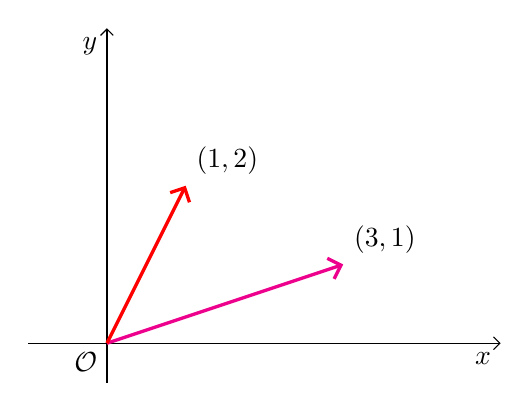
\begin{tikzpicture}[% styles used in image code
         > = Straight Barb, % defined in "arrows.meta
dot/.style = {circle, fill,
              minimum size=2mm, inner sep=0pt, outer sep=0pt,
              node contents={}},
box/.style = {draw, thin, minimum  width=2mm, minimum height=4mm,
              inner sep=0pt, outer sep=0pt,
              node contents={}, sloped},
my angle/.style args = {#1/#2}{draw,->,
                               angle radius=#1,
                               angle eccentricity=#2,
                               } % angle label position!
                        ]
	% coordinate axis
	\draw[->] (-1, 0)   -- (5,0) node[below left] {$x$};
	\draw[->] ( 0,-0.5) -- (0,4) node[below left] {$y$};

	\coordinate (O) at (0,0);
	\coordinate (v1) at (3,1);
	\coordinate (v2) at (1,2);
	
	\draw (O) node[below left] {$\mathcal{O}$};
	\draw [->,magenta,very thick] (O) --(v1) node[above right,black] {$(3,1)$};
	\draw [->,red,very thick] (O) --(v2) node[above right,black] {$(1,2)$};
\end{tikzpicture} \caption*{Arrow representation of two euclidean vectors.}
\end{figure}

\noindent The components of euclidean vectors represented this way are generally called the $x$ and $y$ components (there will be a $z$ component for triples), and so we often write $\mathbf{v}=(v_x, v_y)$. For obvious reasons we also call these 2 dimensional vectors.

Now we would like to create a way to add vectors together. When we add two vectors together the result should also be a vector. 

\definition{Tuple addition}{
Euclidean vectors are added to each other component by component. In symbols
\begin{align*}
(a_1, a_2, \dots, a_n) + (b_1, b_2, \dots, b_n) = (a_1+b_1, a_2+b_2, \dots, a_n + b_n).
\end{align*}
\textit{Note}: this means you can only add two tuples together \textit{of the same size}. It makes no sense to add a 3-tuple to a 5-tuple.
}

\noindent Let's understand this tuple addition geometrically. For the two vectors we represented above, $\mathbf{a}=(1,2)$, $\mathbf{b}=(3,1)$ and so their addition is the vector $\mathbf{c}=\mathbf{a}+\mathbf{b}=(1+3,2+1)=(4,3)$. This component by component addition is represented below left. We can also understand this addition as though we move the vector $\mathbf{b}$ so that its tail is at the tip of $\mathbf{a}$. This tip-to-tail method is shown below to the right. It equally works by moving $\mathbf{a}$ to the tip of $\mathbf{b}$ meaning that $\mathbf{a}+\mathbf{b} = \mathbf{b}+\mathbf{a}$.

\begin{figure}[H]
\centering
\begin{subfigure}[b]{0.45\textwidth}
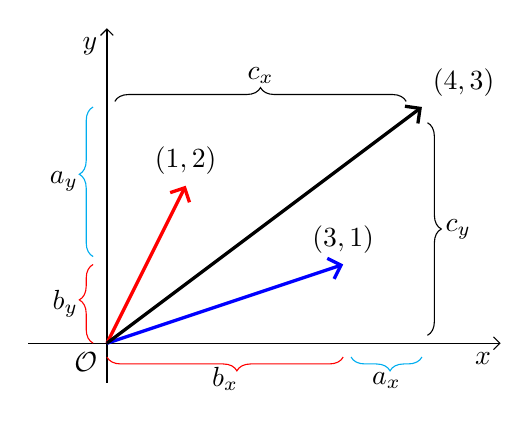
\begin{tikzpicture}[% styles used in image code
         > = Straight Barb, % defined in "arrows.meta
dot/.style = {circle, fill,
              minimum size=2mm, inner sep=0pt, outer sep=0pt,
              node contents={}},
box/.style = {draw, thin, minimum  width=2mm, minimum height=4mm,
              inner sep=0pt, outer sep=0pt,
              node contents={}, sloped},
my angle/.style args = {#1/#2}{draw,->,
                               angle radius=#1,
                               angle eccentricity=#2,
                               } % angle label position!
                        ]
	% coordinate axis
	\draw[->] (-1, 0)   -- (5,0) node[below left] {$x$};
	\draw[->] ( 0,-0.5) -- (0,4) node[below left] {$y$};

	\coordinate (O) at (0,0);
	\coordinate (a) at (1,2);
	\coordinate (ax) at (1,0);
	\coordinate (ay) at (0,2);
	\coordinate (b) at (3,1);
	\coordinate (bx) at (3,0);
	\coordinate (by) at (0,1);
	\coordinate (c) at (4,3);
	\coordinate (cx) at (4,0);
	\coordinate (cy) at (0,3);
	
	\draw (O) node[below left] {$\mathcal{O}$};
	\draw [->,red,very thick] (O) -- (a) node[black, above] {$(1,2)$};
	\draw [->,blue,very thick]  (O) -- (b) node[black, above] {$(3,1)$};
	\draw [->,very thick] (O) -- (c) node[above right] {$(4,3)$};
	
	
	\draw [black, decorate, decoration={brace,amplitude=5pt,raise=2pt,aspect=0.5}] 
		($(cy)+(0.1,0)$)--($(c)-(0.2,0)$) node[pos=0.5,black,above=5pt]{$c_x$};
	\draw [black, decorate, decoration={brace,mirror,amplitude=5pt,raise=2pt,aspect=0.5}] 
		($(cx)+(0,0.1)$) -- ($(c)-(0,0.2)$) node[pos=0.5,black,right=5pt]{$c_y$};
	
	\draw [red, decorate, decoration={brace,mirror,raise=5pt,amplitude=5pt,aspect=0.55}] 
		(O)--(bx) node[pos=0.5,black,below=5pt]{$b_x$};
	
	\draw [red, decorate, decoration={brace,raise=5pt,amplitude=5pt,aspect=0.55}] 
		(O)--(by) node[pos=0.5,black,left=7pt]{$b_y$};
	
	\draw [cyan, decorate, decoration={brace,mirror,raise=5pt,amplitude=5pt,aspect=0.55}] 
		($(bx)+(0.1,0)$)--($(bx)+(ax)$) node[pos=0.5,black,below=7pt]{$a_x$};
	
	\draw [cyan, decorate, decoration={brace,raise=5pt,amplitude=5pt,aspect=0.55}] 
		($(by)+(0,0.1)$)--($(by)+(ay)$) node[pos=0.5,black,left=7pt]{$a_y$};
		
\end{tikzpicture} \caption*{Component by component addition.}
\end{subfigure}
~
\begin{subfigure}[b]{0.45\textwidth}
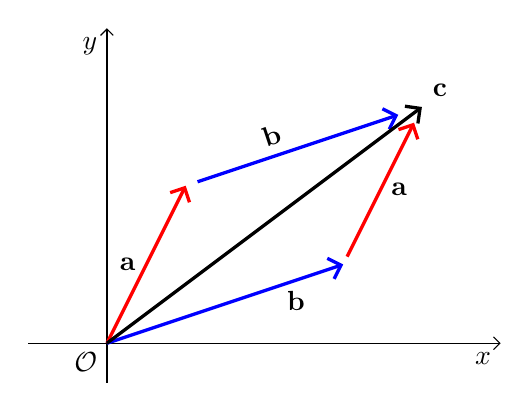
\begin{tikzpicture}[% styles used in image code
         > = Straight Barb, % defined in "arrows.meta
dot/.style = {circle, fill,
              minimum size=2mm, inner sep=0pt, outer sep=0pt,
              node contents={}},
box/.style = {draw, thin, minimum  width=2mm, minimum height=4mm,
              inner sep=0pt, outer sep=0pt,
              node contents={}, sloped},
my angle/.style args = {#1/#2}{draw,->,
                               angle radius=#1,
                               angle eccentricity=#2,
                               } % angle label position!
                        ]
	% coordinate axis
	\draw[->] (-1, 0)   -- (5,0) node[below left] {$x$};
	\draw[->] ( 0,-0.5) -- (0,4) node[below left] {$y$};

	\coordinate (O) at (0,0);
	\coordinate (a) at (1,2);
	\coordinate (b) at (3,1);
	\coordinate (c) at (4,3);
	
	\draw (O) node[below left] {$\mathcal{O}$};
	\draw [->,red,very thick] (O) --(a) node[black,pos=0.5,left] {$\mathbf{a}$};
	\draw [->,blue,very thick] ($(a)+0.05*(b)$) --($(a)+0.9*(b)$) node[black,pos=0.4,rotate=18.4,above] {$\mathbf{b}$};
	\draw [->,blue,very thick] (O) --(b) node[black,pos=0.8,below] {$\mathbf{b}$};
	\draw [->,red,very thick] ($(b)+0.05*(a)$) --($(b)+0.9*(a)$) node[black,pos=0.5,pos=0.5,right] {$\mathbf{a}$};
	\draw [->,very thick] (O) --(c) node[above right] {$\mathbf{c}$};
\end{tikzpicture} \caption*{Tip-to-tail representation.}
\end{subfigure}
\end{figure}

\noindent Now lets think about multiplcation. We can naturally think of doubling or tripling a vector, which should be adding a vector to itself 2 or 3 times, and geometrically it just becomes longer. So we want $2\mathbf{v} = \mathbf{v} + \mathbf{v}$. In components this gives $2(v_x,v_y)=(v_x,v_y) + (v_x,v_y) = (2v_x,2v_y)$. So we see that multiplying a tuple by a number multiplies each of its components by that number.

\definition{Scalar multiplication}{
Let $c\in\mathbb{R}$, called a scalar quantity, and $\mathbf{v} \in \mathbb{R}^n$ with components $v_i$. Then the \textit{scalar multiplication} $c\mathbf{v}$ gives a vector $\mathbf{w}$ with components $w_i = c v_i$ for every index $i$. In tuple form
\begin{align*}
c(v_1,v_2,\dots,v_n) = (cv_1,cv_2,\dots,cv_n).
\end{align*}
}

\begin{figure}[H]
\centering
\begin{tikzpicture}[% styles used in image code
         > = Straight Barb, % defined in "arrows.meta
dot/.style = {circle, fill,
              minimum size=2mm, inner sep=0pt, outer sep=0pt,
              node contents={}},
box/.style = {draw, thin, minimum  width=2mm, minimum height=4mm,
              inner sep=0pt, outer sep=0pt,
              node contents={}, sloped},
my angle/.style args = {#1/#2}{draw,->,
                               angle radius=#1,
                               angle eccentricity=#2,
                               } % angle label position!
                        ]
	% coordinate axis
	\draw[->] (-3, 0)   -- (5,0) node[below left] {$x$};
	\draw[->] ( 0,-1) -- (0,3) node[below left] {$y$};

	\coordinate (O) at (0,0);
	\coordinate (v1) at (2,1);
	\coordinate (v2) at (1,0.5);
	\coordinate (v3) at (4,2);
	\coordinate (v4) at (-2,-1);
	
	\draw (O) node[below right] {$\mathcal{O}$};
	\draw [->,blue] (O) --(v3) node[pos=0.7,above,black] {$2\mathbf{v}$};
	\draw [->,black] (O) --(v1) node[pos=0.78,above,black] {$\mathbf{v}$};
	\draw [->,magenta,very thick] (O) --(v2) node[pos=0.5,above=5pt,black] {$0.5\mathbf{v}$};
	\draw [->,red] (O) --(v4) node[pos=0.7,above,black] {$-1\mathbf{v}$};
\end{tikzpicture} \caption*{Arrow representation of scalar multiplication.}
\end{figure}

\noindent We can use scalar multiplication and some manipulation to form a second way to represent Euclidean vectors:
\begin{align*}
(v_1,v_2,\dots,v_n) &= (v_1,0,\dots,0) + (0,v_2,\dots,0) + \cdots + (0,0,\dots,v_n) \\
&= v_1(1,0,\dots,0) + v_2(0,1,\dots,0) + \cdots + v_n(0,0,\dots,1)\\
&= v_1\mathbf{e}_1 + v_2\mathbf{e}_2 + \cdots + v_n\mathbf{e}_n
\end{align*}
where we have introduced the canonical Euclidean vectors.

\definition{Canonical Euclidean unit vectors}{
The canonical Euclidean vectors in $\mathbb{R}^n$ are the $n$ vectors of the form
\begin{gather*}
\mathbf{e}_1 = (1,0,\dots,0) \\
\mathbf{e}_2 = (0,1,\dots,0) \\
\vdots \\
\mathbf{e}_n = (0,0,\dots,1).
\end{gather*}
More compactly
\begin{align*}
\mathbf{e}_k = (\alpha_1, \alpha_2, \dots, \alpha_n) \quad \text{where} \quad
\alpha_j=
\begin{cases}
1 & \text{for } j= k, \\
0 & \text{for } j\neq k.
\end{cases}
\end{align*}
}

\noindent In two dimensions we have several notations for these unit vectors
\begin{align*}
\mathbf{v} = v_x \hat{x} + v_y \hat{y} = v_x \mathbf{e}_x + v_y \mathbf{e}_y = v_x \hat{i} + v_y \hat{j}
\end{align*}
but we will stick to the hat notation, $\hat{x}$, in this text when referring to the geometric representations in 2 or 3d ($\hat{z}=\mathbf{e}_z = \hat{k}$ being used for the third direction). We can understand these unit vectors as the building blocks of the arrow:
\begin{figure}[H]
\centering
\begin{tikzpicture}[% styles used in image code
         > = Straight Barb, % defined in "arrows.meta
dot/.style = {circle, fill,
              minimum size=2mm, inner sep=0pt, outer sep=0pt,
              node contents={}},
box/.style = {draw, thin, minimum  width=2mm, minimum height=4mm,
              inner sep=0pt, outer sep=0pt,
              node contents={}, sloped},
my angle/.style args = {#1/#2}{draw,->,
                               angle radius=#1,
                               angle eccentricity=#2,
                               } % angle label position!
                        ]
	% coordinate axis
	\draw[->] (-3, 0)   -- (5,0) node[below] {$x$};
	\draw[->] ( 0,-1) -- (0,3.5) node[left] {$y$};

	\coordinate (O) at (0,0);
	\coordinate (v) at (2,3);
	\coordinate (xhat) at (1,0);
	\coordinate (yhat) at (0,1);
	
	\draw (O) node[below left] {$\mathcal{O}$};
	\draw [->] (O) --(v) node[pos=0.9,above left,rotate=56.3] {$\mathbf{v}=(2,3)$};
	\draw [->, blue] (O) --(xhat) node[pos=0.5,below=5pt] {$\hat{x}$};
	\draw [->, blue] (xhat) --($2*(xhat)$) node[pos=0.5,below=5pt] {$\hat{x}$};
	\draw [->, magenta] (O) --(yhat) node[pos=0.5,left=5pt] {$\hat{y}$};
	\draw [->, magenta] ($2*(xhat)$) --($2*(xhat)+(yhat)$) node[pos=0.5,right=5pt] {$\hat{y}$};
	\draw [->, magenta] ($2*(xhat)+(yhat)$) --($2*(xhat)+2*(yhat)$) node[pos=0.5,right=5pt] {$\hat{y}$};
	\draw [->, magenta] ($2*(xhat)+2*(yhat)$) --($2*(xhat)+3*(yhat)$) node[pos=0.5,right=5pt] {$\hat{y}$};
\end{tikzpicture} \caption*{Unit vectors as building blocks of a Euclidean vector.}
\end{figure}

\section{Dot product}

\noindent Notice that with scalar multiplication we multiplied two different kinds of objects together, a scalar by a vector resulting in a vector. How about multiplying two vectors together? You might be tempted to simply form a new vector with component by component multiplication, as we did for addition. This turns out not to be so useful. One very useful way to define vector multiplication is as follows.

\definition{Dot product}{
For two $n$-tuples $\mathbf{a}$ and $\mathbf{b}$, their \textit{dot product}, also called \textit{scalar} product and \textit{Euclidean inner} product, is the real number given by the addition of component by component multiplication
\begin{align*}
\mathbf{a}\cdot\mathbf{b} = a_1 b_1 + a_2 b_2 + \cdots + a_n b_n = \sum_{i=1}^n a_i b_i.
\end{align*}
}

\noindent Notice that the result of this product is a real number, not another tuple. Let's first try to understand the dot product by considering a 2d vector ``dotted'' with itself:
\begin{align*}
\mathbf{v}\cdot\mathbf{v}=(v_x,v_y)\cdot(v_x,v_y)=v_x^2 + v_y^2.
\end{align*}
This dot product gives the square of the length of the right triangle made from the $x$ and $y$ components of $\mathbf{v}$:

\begin{figure}[H]
\centering
\begin{tikzpicture}[% styles used in image code
         > = Straight Barb, % defined in "arrows.meta
dot/.style = {circle, fill,
              minimum size=2mm, inner sep=0pt, outer sep=0pt,
              node contents={}},
box/.style = {draw, thin, minimum  width=2mm, minimum height=4mm,
              inner sep=0pt, outer sep=0pt,
              node contents={}, sloped},
my angle/.style args = {#1/#2}{draw,->,
                               angle radius=#1,
                               angle eccentricity=#2,
                               } % angle label position!
                        ]
	% coordinate axis
	%\draw[->] (-3, 0)   -- (5,0) node[below left] {$x$};
	%\draw[->] ( 0,-1) -- (0,3) node[below left] {$y$};

	\coordinate (O) at (0,0);
	\coordinate (v1) at (6,4);
	\coordinate (vx) at (6,0);
	\coordinate (vy) at (0,4);
	
	\draw [->] (O) --(v1) node[pos=0.5,above=5pt] {$\mathbf{v}$};
	\draw [dashed] (O) --($(vx)-(0.1,0)$) node[pos=0.5,below] {$v_x$};
	\draw [dashed] (vx) --($(v1)-(0,0.15)$) node[pos=0.5,right] {$v_y$};
\end{tikzpicture} \caption*{Components of the vector $\mathbf{v}$}
\end{figure}

\noindent So we can identify the dot product $\mathbf{v}\cdot\mathbf{v}$ with the square of the length of $\mathbf{v}$. We generalise this concept of vector length in the operation of the norm.

\definition{Norm}{
The norm of an $n$-tuple $\mathbf{v}$, denoted $\lVert \mathbf{v} \rVert$, is given by
\begin{align*}
\lVert \mathbf{v} \rVert = \sqrt{\mathbf{v}\cdot\mathbf{v}} = \sqrt{v_1^2 + v_2^2 + \cdots + v_2^2}.
\end{align*}
}

\noindent So far we have defined a vector by its components. Through the norm, we can have a method of \textit{calculating} the components from 2 other pieces of information: its length and its direction. Its direction will mean its angle with respect to the $x$-axis. Denote that angle $\theta$ and the norm as the non-bold font version of the vector $v=\lVert \mathbf{v} \rVert$. From the above figure, we see that $\cos\theta = v_x/v$ and $\sin\theta = v_y/v$. So, given a vector length and its direction we have
\begin{align*}
\mathbf{v} = (v\cos\theta, v\sin\theta) = v(\cos\theta,\sin\theta).
\end{align*}
This gives us the following result: for any 2d Euclidean vector $\mathbf{v}$ its components are given by
\begin{align*}
v_x &= \lVert \mathbf{v} \rVert \cos\theta \\
v_y &= \lVert \mathbf{v} \rVert \sin\theta
\end{align*}
where $\theta$ is the angle that $\mathbf{v}$ makes with the $x$ axis.

\noindent What happens if we dot two different vectors with this representation. Let $\mathbf{a}=a(\cos\alpha,\sin\alpha)$ and $\mathbf{b}=b(\cos\beta,\sin\beta)$. Then
\begin{align*}
\mathbf{a}\cdot\mathbf{b} &= [a(\cos\alpha,\sin\alpha)]\cdot [b(\cos\beta,\sin\beta)] \\
&= ab(\cos\alpha,\sin\alpha)\cdot (\cos\beta,\sin\beta) \\
&= ab(\cos\alpha\cos\beta + \sin\alpha\sin\beta) \\
&= ab \cos(\alpha-\beta)
\end{align*}
where we have used a trigonometric identity in the last line and a little trickery in the first line that you should verify: $(c_1\mathbf{v}_1)\cdot(c_2\mathbf{v}_2)=(c_1c_2)\mathbf{v}_1\cdot\mathbf{v}_2$. In the end we have shown the following theorem.

\theorem{Dot product with angle}{
The Euclidean dot product of two $n$-tuples $\mathbf{a}$ and $\mathbf{b}$ can be calculated solely from their norms and the angle between them, $\theta$, given by the formula
\begin{align*}
\mathbf{a}\cdot\mathbf{b} = \lVert \mathbf{a} \rVert \lVert \mathbf{b} \rVert \cos \theta
\end{align*}
}
\begin{figure}[H]
\centering
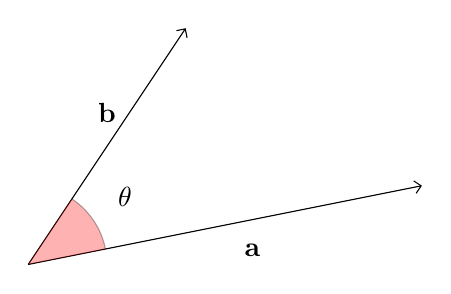
\begin{tikzpicture}[% styles used in image code
         > = Straight Barb, % defined in "arrows.meta
dot/.style = {circle, fill,
              minimum size=2mm, inner sep=0pt, outer sep=0pt,
              node contents={}},
box/.style = {draw, thin, minimum  width=2mm, minimum height=4mm,
              inner sep=0pt, outer sep=0pt,
              node contents={}, sloped},
my angle/.style args = {#1/#2}{draw,->,
                               angle radius=#1,
                               angle eccentricity=#2,
                               } % angle label position!
                        ]
	% coordinate axis
	%\draw[->] (-3, 0)   -- (5,0) node[below left] {$x$};
	%\draw[->] ( 0,-1) -- (0,3) node[below left] {$y$};

	\coordinate (O) at (0,0);
	\coordinate (a) at (5,1);
	\coordinate (b) at (2,3);
	
	\draw [->] (O) --(a) node[pos=0.5,below right=5pt] {$\mathbf{a}$};
	\draw [->] (O) --(b) node[pos=0.5,above=5pt] {$\mathbf{b}$};
	
	\begin{scope}
	\path[clip] (O) -- (a) -- (b);
	\fill[red, opacity=0.3, draw=black] (O) circle (10mm);
	\node at ($(O)+(35:15mm)$) {$\theta$};
	\end{scope}
\end{tikzpicture}\caption*{The angle between two vectors.}
\end{figure}

\noindent From this expression of the dot product we see immediately what happens in the special case of perpendicular vectors. When two vectors are perpendicular the angle between them is $\pi/2$ and the dot product is then zero (recall that $\cos(\pi/2)=0$). We can extend this result to define orthogonality for higher dimensional Euclidean vectors.

\definition{Orthogonal Euclidean vectors}{
Two vectors in $\mathbb{R}^n$ are orthogonal if and only if their dot product equals zero.
}

\section{Applications}

So far we have been considering Euclidean vectors as arrows pointing from the origin to the given tuple. It can be useful to consider arrows pointing from an arbitrary point in space to another.

\definition{Displacement vector}{
Given two Euclidean vectors $\mathbf{a}$ and $\mathbf{b}$, the displacement vector pointing from $\mathbf{a}$ to $\mathbf{b}$ is given by $\mathbf{r}=\mathbf{b}-\mathbf{a}$ as pictured below. Of course we can also create the displacement vector in the other direction, from $\mathbf{b}$ to $\mathbf{a}$, given by $\mathbf{a}-\mathbf{b}$.
}

\begin{figure}[H]
\centering
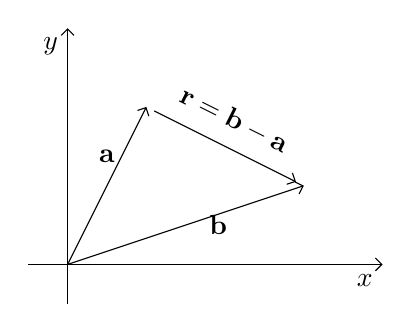
\begin{tikzpicture}[% styles used in image code
         > = Straight Barb, % defined in "arrows.meta
dot/.style = {circle, fill,
              minimum size=2mm, inner sep=0pt, outer sep=0pt,
              node contents={}},
box/.style = {draw, thin, minimum  width=2mm, minimum height=4mm,
              inner sep=0pt, outer sep=0pt,
              node contents={}, sloped},
my angle/.style args = {#1/#2}{draw,->,
                               angle radius=#1,
                               angle eccentricity=#2,
                               } % angle label position!
                        ]
	% coordinate axis
	\draw[->] (-0.5, 0) -- (4,0) node[below left] {$x$};
	\draw[->] ( 0,-0.5) -- (0,3) node[below left] {$y$};

	\coordinate (O) at (0,0);
	\coordinate (a) at (1,2);
	\coordinate (b) at (3,1);
	\coordinate (ar) at ($0.95*(a)+0.05*(b)$);
	\coordinate (br) at ($0.95*(b)+0.05*(a)$);
	
	\draw [->] (O) --(a) node[pos=0.5,above=5pt] {$\mathbf{a}$};
	\draw [->] (O) --(b) node[pos=0.5,right=5pt] {$\mathbf{b}$};
	\draw [->] (ar) --(br) node[pos=0.5,above=3pt,rotate=-26.5] {$\mathbf{r}= \mathbf{b}-\mathbf{a}$};
\end{tikzpicture}
\end{figure}

Why is this useful? Well we can, for example, represent straight lines in a new way. Recall the equation for a straight line $y=mx+b$ where $m$ gives the slope of the line and $b$ gives the $y$-intercept (or vertical offset). Let's consider the line $y=(0.5)x+1$. Now that means we can choose any two $x$ values, say $x=-1$ and $x=2$, and compute corresponding $y$ values, in this case $y=0.5$ and $y=2$. So the Euclidean vectors $\mathbf{a}=(-1,0.5)$ and $\mathbf{b}=(2,2)$ belong to the line, as pictured.

\begin{figure}[H]
\centering
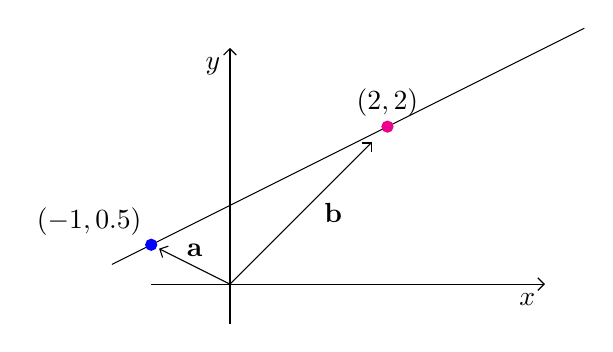
\begin{tikzpicture}[% styles used in image code
         > = Straight Barb, % defined in "arrows.meta
dot/.style = {circle, fill,
              minimum size=2mm, inner sep=0pt, outer sep=0pt,
              node contents={}},
box/.style = {draw, thin, minimum  width=2mm, minimum height=4mm,
              inner sep=0pt, outer sep=0pt,
              node contents={}, sloped},
my angle/.style args = {#1/#2}{draw,->,
                               angle radius=#1,
                               angle eccentricity=#2,
                               } % angle label position!
                        ]
	% coordinate axis
	\draw[->] (-1, 0) -- (4,0) node[below left] {$x$};
	\draw[->] ( 0,-0.5) -- (0,3) node[below left] {$y$};
	
	\draw[domain=-1.5:4.5,variable=\x] plot({\x},{0.5*\x+1});

	\coordinate (O) at (0,0);
	\coordinate (a) at (-1,0.5);
	\coordinate (b) at (2,2);
	
	\draw [->] (O) --($0.9*(a)$) node[pos=0.5,above] {$\mathbf{a}$};
	\draw [->] (O) --($0.9*(b)$) node[pos=0.5,right=5pt] {$\mathbf{b}$};
	
	\filldraw [blue] (a) circle (2pt) node[above left,black] (a) {$(-1,0.5)$};
	\filldraw [magenta] (b) circle (2pt) node[above,black] (b) {$(2,2)$};
\end{tikzpicture}
\end{figure}

\noindent The displacement vector from $\mathbf{a}$ to $\mathbf{b}$ is given by $\mathbf{r}=\mathbf{b}-\mathbf{a}=(2,2)-(-1,0.5)=(3,1.5)$. This displacement vector can be used to represent any point on the line. We just have to start at $\mathbf{a}$ and add any multiple of $\mathbf{r}$:


\begin{figure}[H]
\centering
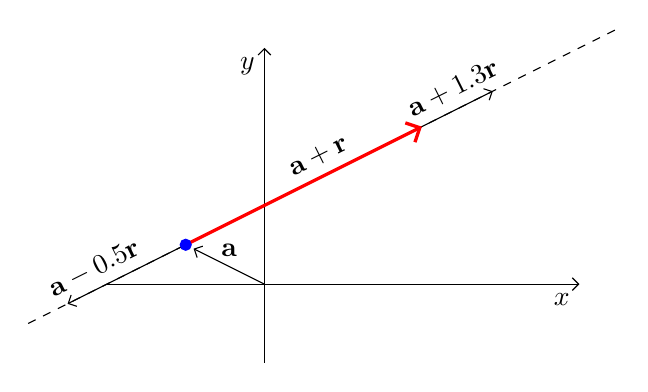
\begin{tikzpicture}[% styles used in image code
         > = Straight Barb, % defined in "arrows.meta
dot/.style = {circle, fill,
              minimum size=2mm, inner sep=0pt, outer sep=0pt,
              node contents={}},
box/.style = {draw, thin, minimum  width=2mm, minimum height=4mm,
              inner sep=0pt, outer sep=0pt,
              node contents={}, sloped},
my angle/.style args = {#1/#2}{draw,->,
                               angle radius=#1,
                               angle eccentricity=#2,
                               } % angle label position!
                        ]
	% coordinate axis
	\draw[->] (-2, 0) -- (4,0) node[below left] {$x$};
	\draw[->] ( 0,-1) -- (0,3) node[below left] {$y$};
	
	\draw[dashed,domain=-3:4.5,variable=\x] plot({\x},{0.5*\x+1});

	\coordinate (O) at (0,0);
	\coordinate (a) at (-1,0.5);
	\coordinate (r) at (3,1.5);
	
	\draw [->] (O) --($0.9*(a)$) node[pos=0.5,above] {$\mathbf{a}$};
	\draw [->] (a) --($(a)+1.3*(r)$) node[pos=0.9,above,rotate=26.5] {$\mathbf{a}+1.3\mathbf{r}$};
	\draw [->,red,very thick] (a) --($(a)+(r)$) node[pos=0.6,above,rotate=26.5,black] {$\mathbf{a}+\mathbf{r}$};
	\draw [->] (a) --($(a)-0.5*(r)$) node[pos=0.7,above,rotate=26.5] {$\mathbf{a}-0.5\mathbf{r}$};
	
	\filldraw [blue] (a) circle (2pt);
\end{tikzpicture}
\end{figure}
\noindent So this gives as the vector representation of a line.

\definition{Vector form of a straight line}{
The set of vectors in $\mathbb{R}^n$ of the form $\mathbf{v} = \mathbf{a} + t \mathbf{r}$ for a parameter $t\in\mathbb{R}$ represents a straight line through the space $\mathbb{R}^n$. That is,
\begin{align*}
\{(x,y) \, | \, \forall x\in\mathbb{R} \, \text{and} \, y=mx+b  \} = \{ \mathbf{a} + t \mathbf{r} \, | \, \forall t\in\mathbb{R} \}
\end{align*}
where $\mathbf{a}$ is an arbitrary pair $(x,mx+b)$ and $\mathbf{r}$ is a displacement vector between any two distinct pairs $(x_1,mx_1+b)$ and $(x_2,mx_2+b)$.
}


\section*{To do}
Unit vector

unit vector pointing in the direction of a given vector

Dot product as projection into another direction

\section{Summary of properties of Euclidean vectors}\label{sec:ch1_summary}

Let's collect a list of key properties of operations with tuples that will turn out not to be unique to tuples. The following are true for any tuples $\mathbf{a}$, $\mathbf{b}$ and $\mathbf{c} \in\mathbb{R}^n$ and any real numbers $k$ and $l\in\mathbb{R}$.

\begin{align*}
& \text{addition of tuples gives another tuple} && \quad \mathbf{a} + \mathbf{b} \in \mathbb{R}^n &\\
%
& \text{tuple addition is associative} && \quad (\mathbf{a} + \mathbf{b}) + \mathbf{c}  =\mathbf{a} + (\mathbf{b} + \mathbf{c}) &\\
%
& \text{the zero tuple is a tuple of zeros} && \quad \mathbf{a} + \mathbf{0} = \mathbf{0} + \mathbf{a} = \mathbf{a} &\\
%
& \text{the negative of a tuple is the additive inverse} && \quad \mathbf{a} + (-\mathbf{a}) = \mathbf{0} &\\
%
& \text{the order of tuple addition doesn't matter} && \quad \mathbf{a} + \mathbf{b} = \mathbf{b} + \mathbf{a} &\\
%
& \text{scalar multiplication of a tuple gives another tuple} && \quad k\mathbf{a} \in \mathbb{R}^n &\\
%
& \text{scalar multiplication distributes of tuple addition} && \quad k(\mathbf{a}+\mathbf{b})=k\mathbf{a}+k\mathbf{b} &\\
%
& \text{scalar addition distributes over tuples} && \quad (k+l)\mathbf{a}=k\mathbf{a}+l\mathbf{a} &\\
%
& \text{scalar multiplication order doesn't matter} && \quad k(l\mathbf{a})=(kl)\mathbf{a} &\\
%
& \text{scalar multiplication by 1 is an identity operation} && \quad 1\mathbf{a}=\mathbf{a} &
\end{align*}
%\chapter{Matrix Algebra} \label{ch:matrixalgebra}

\section{Basic Definitions}

\definition{Matrix}{
A matrix is a collection of numbers from a field $\mathbb{F}$ (e.g. rational numbers) usually represented by a rectangular array. For example, an $m \times n$ (said m by n) matrix $A$ with coefficients $a_{ij}\in\mathbb{F}$  would be represented by an array with $m$ rows and $n$ columns:
\begin{align*}
A = 
\begin{pmatrix}
a_{11} & a_{12} & a_{13} & \cdots & a_{1j} & \cdots & a_{1m} \\
a_{21} & a_{22} & a_{23} & \cdots & a_{2j} & \cdots & a_{2m} \\
a_{31} & a_{32} & a_{33} & \cdots & a_{3j} & \cdots & a_{3m} \\
\vdots & \vdots & \vdots & \ddots & \vdots & \ddots & \vdots \\
a_{i1} & a_{12} & a_{13} & \cdots & a_{ij} & \cdots & a_{im} \\
\vdots & \vdots & \vdots & \ddots & \vdots & \ddots & \vdots \\
a_{n1} & a_{n2} & a_{n3} & \cdots & a_{nj} & \cdots & a_{nm}
\end{pmatrix}
=
\left( a_{ij} \right)_{\substack{ 1 \leq i \leq m \\ 1 \leq j \leq n }}.
\end{align*}
Sometimes it is convenient to refer to the coefficients in the array like so: $a_{ij} = \left(A\right)_{ij}$.
}

\definition{Set of all $m \times n$ matrices}{
We write the set of all $m \times n$ matrices with coefficients in $\mathbb{F}$ as
\begin{align*}
\mathcal{M}_{m,n}(\mathbb{F})
\end{align*}
}

\noindent It is sometimes useful in calculations to use the columns or rows of a matrix, and so we create the following notation.

\definition{Matrix columns and rows}{
For a matrix $A\in\mathcal{M}_{m,n}(\mathbb{F})$ we denote its j$^{th}$ column and i$^{th}$ row
\begin{align*}
A^{(j)} =
\begin{pmatrix}
 a_{1j} \\
 a_{2j} \\
 a_{3j} \\
 \vdots \\
 a_{ij} \\
 \vdots \\
 a_{mj}
\end{pmatrix},
\qquad
A_{(i)} =
\begin{pmatrix}
a_{i1} & a_{12} & a_{13} & \cdots & a_{ij} & \cdots & a_{in}
\end{pmatrix}
\end{align*}
}

\noindent For the rest of this course, unless otherwise noted, we will implicitly assume real matrices by writing $\mathcal{M}_{m,n}(\mathbb{R}) = \mathcal{M}_{m,n}$.

\definition{Transpose of a matrix}{
The transpose of an $m \times n$ matrix, $A$, is an $n \times m$ matrix, denoted $A^T$, with rows equal to the columns of $A$. That is, $\left(A^T\right)_{ij} = \left(A\right)_{ji}$ for all combinations of $i$ and $j$. 
}

\noindent For example
\begin{align*}
\begin{pmatrix}
1  & -2  \\
0  & -1  \\
-1 &  0
\end{pmatrix}^T
=
\begin{pmatrix}
 1  &  0 & -1\\
-2  & -1 &  0
\end{pmatrix}
\end{align*}


\definition{Diagonal matrix}{
A square matrix $A$ is said to be diagonal if all its non-diagonal elements are zero, e.g. $(A)_{ij}=0$ whenever $i \neq j$.
}

\definition{Symmetric matrix}{
A matrix $A$ is symmetric if it is equal to its transpose, $A = A^T$.
}


\noindent For example:
\begin{align*}
&\begin{pmatrix}
1.5 & 3 & \pi \\
3   & 2 & 2 \\
\pi & 2 & 1
\end{pmatrix}^T
=
\begin{pmatrix}
1.5 & 3 & \pi \\
3   & 2 & 2 \\
\pi & 2 & 1
\end{pmatrix}
\quad \text{symmetric} \\
%
&\begin{pmatrix}
1.5 & 1 & \pi \\
3   & 2 & 2 \\
7 & 2 & 1
\end{pmatrix}^T
=
\begin{pmatrix}
1.5 & 3 & 7 \\
1   & 2 & 2 \\
\pi & 2 & 1
\end{pmatrix}
\quad \text{not symmetric}
\end{align*}

\section{Matrix addition and scalar multiplication}


\definition{Matrix addition}{
Matrix addition is done coefficient by coefficient, that is, for two matrices $A$ and $B$ we define the i,j$^{th}$ coefficient of the addition as the addition of the i,j$^{th}$ coefficients of each matrix: 
\begin{align*}
\left(A+B\right)_{ij} = \left(A\right)_{ij}+\left(B\right)_{ij}.
\end{align*}
}

\noindent For example
\begin{align*}
\begin{pmatrix}
1 &  2 & -2 \\
3 & -1 & 0   
\end{pmatrix}
+
\begin{pmatrix}
0 & -1 & 3 \\
2 &  0 & 3   
\end{pmatrix}
=
\begin{pmatrix}
1+0 & 2-1 & -2+3 \\
3+2 & -1+0 & 0+3   
\end{pmatrix}
=
\begin{pmatrix}
1 &  1 & 1 \\
5 & -1 & 3   
\end{pmatrix}.
\end{align*}
This definition means that matrix addition is only well defined if the matrices have the same shape. It also implies that any two matrices $A,B \in \mathcal{M}_{m,n}$ add to give a third matrix $C \in \mathcal{M}_{m,n}$. That is, $\mathcal{M}_{m,n}$ is closed under addition with this definition.

\theorem{Matrix addition is associative}{ 
Given three matrices $A,B,C \in \mathcal{M}_{m,n}$:
\begin{align*}
A + (B + C) = (A + B) + C
\end{align*}
}

\begin{proof}
Let $D = B + C$, so that the definition of matrix addition gives us 
\begin{align*}
(D)_{ij}=(B)_{ij} + (C)_{ij}.
\end{align*}
Then $A + (B + C)= A + D$ has coefficients 
\begin{align*}
(A)_{ij} + (D)_{ij} = (A)_{ij} + ((B)_{ij} + (C)_{ij}).
\end{align*}
Addition in fields is associative, so
\begin{align*}
(A)_{ij} + ((B)_{ij} + (C)_{ij}) = ((A)_{ij} + (B)_{ij}) + (C)_{ij}
\end{align*}
These are exactly the coefficients of $(A+B)+C$.
\end{proof}

\theorem{Matrix addition is commutative}{ 
Given two matrices $A,B \in \mathcal{M}_{m,n}$:
\begin{align*}
A + B = B + A
\end{align*}
}



\definition{Scalar multiplication}{
Given a number $k\in\mathbb{R}$ (called a scalar) and a matrix $A \in \mathcal{M}_{m,n}$, we define matrix scalar multiplication, $kA$, to be a matrix $B \in \mathcal{M}_{m,n}$ with coefficients given by:
\begin{align*}
b_{ij} = ka_{ij},
\end{align*}
that is, we multiply \textit{every coefficient} by the scalar.
} 

\noindent For example:
\begin{gather*}
k
\begin{pmatrix}
 1 & 3 \\
 7 & 2 
\end{pmatrix}
=
\begin{pmatrix}
 k & 3k \\
 7k & 2k 
\end{pmatrix}
%%%%%%%%
%%%%%%%%
\\
%%%%%%%%
%%%%%%%%
\frac{1}{2}
\begin{pmatrix}
 2 & 2 \\
 1 & 1 \\
 0 & 3 
\end{pmatrix}
=
\begin{pmatrix}
 1 & 1 \\
 1/2 & 1/2 \\
 0 & 3/2 
\end{pmatrix}
\end{gather*}

\theorem{Scalar multiplication is distributive}{
For any scalars $\alpha,\beta \in \mathbb{R}$ and matrices $A,B \in \mathcal{M}_{n,m}$, scalar multiplication on matrices is both distributive over matrix addition:
\begin{align*}
\alpha(A + B) = \alpha A + \alpha B
\end{align*}
and distributive over scalar addition
\begin{align*}
(\alpha + \beta)A = \alpha A + \beta A.
\end{align*}
}

\theorem{Scalar multiplication is associative}{
For any scalars $\alpha,\beta \in \mathbb{R}$ and matrix $A$, scalar multiplication is associative in the following sense:
\begin{align*}
\alpha(\beta A) = (\alpha \beta ) A.
\end{align*}
}

The concept of zero is fundamentally that when we add zero to something we get back the same thing. For matrices then we want, for a matrix $A$, that $A + M_0 = A$. First this means this zero object must be a matrix of the same shape as $A$. Looking at coefficients, we have
\begin{align*}
(A + M_0)_{ij} = (A)_{ij} + (M_0)_{ij} = A_{ij} \implies (M_0)_{ij} = 0
\end{align*}
This gives the following definition.

\definition{Zero matrix}{
The zero matrix of any shape is a matrix $M_0 \in\mathcal{M}_{m,n}$ consisting entirely of zeros as coefficients.
} 
Note that this means there is no unique zero matrix, but rather a zero matrix for every possible matrix shape.

\example{Zero matrices}{
\begin{align*}
\begin{pmatrix}
0 & 0 & 0 & 0 \\
0 & 0 & 0 & 0 
\end{pmatrix}
\quad\quad
\begin{pmatrix}
0 & 0 \\
0 & 0 \\
0 & 0 
\end{pmatrix}
\end{align*}
}

With this zero matrix we can find the additive inverse of a matrix, $A\in\mathcal{M}_{m,n}$, by considering the defining relation $A+B=M_0$, where $B$ is the additive inverse of $A$. This means
\begin{align*}
(A+B)_{ij} = (A)_{ij}+(B)_{ij} = 0 \implies (B)_{ij} = - (A)_{ij} = (-A)_{ij}
\end{align*}

\definition{Additive inverse}{
Given a matrix $A\in\mathcal{M}_{ij}$, its additive inverse is the same matrix multiplied by the scalar $-1$. We denote the additive inverse of $A$ as $-A$.
} 

\example{Additive inverses}{
\begin{gather*}
A=
\begin{pmatrix}
2 & 0 & -1 \\
0 & 1 &  3 
\end{pmatrix}
\quad\implies\quad
-A=
\begin{pmatrix}
 -2 &  0 &  1 \\
  0 & -1 & -3 
\end{pmatrix}
\\
B=
\begin{pmatrix}
  3 & -1 \\
\pi &  0 
\end{pmatrix}
\quad\implies\quad
-B=
\begin{pmatrix}
  -3 &  1 \\
-\pi &  0 
\end{pmatrix}
\end{gather*}
}





\subsection*{Summary of properties of matrix addition and scalar multiplication}

Let's collect a list of key properties of operations with matrices that are shared with tuples. The following are true for any matrices $A,B,C\in\mathcal{M}_{m,n}$ and any real numbers $k$ and $l\in\mathbb{R}$.

\begin{align*}
& \text{addition of matrices gives another matrix} && \quad A + B \in\mathcal{M}_{m,n} &\\
%
& \text{matrix addition is associative} && \quad (A + B) + C = A + (B + C) &\\
%
& \text{the zero matrix is a matrix of zeros} && \quad A + M_0 = M_0 + A = A &\\
%
& \text{the negative of a matrix is the additive inverse} && \quad A + (-A) = M_0 &\\
%
& \text{the order of matrix addition doesn't matter} && \quad A + B = B + A &\\
%
& \text{scalar multiplication of a matrix gives another matrix} && \quad kA\in\mathcal{M}_{m,n} &\\
%
& \text{scalar multiplication distributes of matrix addition} && \quad k(A+B)=kA+kB &\\
%
& \text{scalar addition distributes over matrix} && \quad (k+l)A=kA+lA &\\
%
& \text{scalar multiplication order doesn't matter} && \quad k(lA)=(kl)A &\\
%
& \text{scalar multiplication by 1 is an identity operation} && \quad 1A=A &
\end{align*}


\section{Multiplication of matrices by columns}

When restricting ourselves to simple addition of matrices or scalar multiplication we see that matrices and tuples have the same rules. In fact we could simply think of tuples as $2\times 1$ or $1\times 2$ matrices. Here we will introduce a new type of multiplication, that of matrices by matrices. This is not the same as the dot product.

\definition{Multiplication of a matrix by a column}{
Consider a matrix $A \in \mathcal{M}_{m,n}$ and a column $X \in \mathcal{M}_{n,1}$. We define the product $AX$ to result in the column $Y\in\mathcal{M}_{m,1}$ with coefficients
\begin{align*}
(Y)_i = a_{i1}x_1 + a_{i2}x_2 + \cdots + a_{im}x_m = \sum_{k=1}^m a_{ik} x_k 
\end{align*}
Visually
\begin{align*}
\begin{pmatrix}
y_{1} \\
y_{2} \\
\vdots \\
y_{n} 
\end{pmatrix}
%%%
%%%
%%%
&=
%%%
\begin{pmatrix}
a_{11} & a_{12} & \cdots & a_{1m} \\
a_{21} & a_{22} & \cdots & a_{2m} \\
\vdots & \vdots & \ddots & \vdots \\
a_{n1} & a_{n2} & \cdots & a_{nm}
\end{pmatrix}
\begin{pmatrix}
x_{1} \\
x_{2} \\
\vdots \\
x_{m} 
\end{pmatrix}
%%%
%%%
%%%
=
%%%
x_{1}
\begin{pmatrix}
a_{11} \\
a_{21} \\
\vdots \\
a_{n1} 
\end{pmatrix}
+
x_{2}
\begin{pmatrix}
a_{12} \\
a_{22} \\
\vdots \\
a_{n2} 
\end{pmatrix}
+ \cdots +
x_m
\begin{pmatrix}
a_{1m} \\
a_{2m} \\
\vdots \\
a_{nm} 
\end{pmatrix}
\\ \\
%%%
%%%
%%%
&\implies Y = x_{1}A^{(1)} + x_{2}A^{(2)} + \cdots + x_{m}A^{(m)}
\end{align*}
}

\noindent Notice that in this definition, to be able to multiply a matrix by a column the matrix must have the same number of columns as the elements of the column. Additionally, the answer will be a column of the same shape as the columns of the matrix, \textit{not the column that is multipled by the matrix}.

\noindent Note also that not only is multiplication of matrices by columns not commutative, $AX \neq XA$, but that the latter is not even defined. We cannot multiply a column by a matrix left to right.

\example{Matrix multiplication by columns}{
\begin{align*}
& \begin{pmatrix}
      1 &  2 & 4  \\
      3 & -1 & 0
\end{pmatrix}
\begin{pmatrix}
      3 \\
     -1 \\
      2
\end{pmatrix}
=
3\begin{pmatrix}
1 \\
3
\end{pmatrix}
-
1\begin{pmatrix}
2 \\
-1
\end{pmatrix}
+
2\begin{pmatrix}
4 \\
0
\end{pmatrix}
=
\begin{pmatrix}
 9 \\
 10
\end{pmatrix} \\
%%%%%
%%%%%
%%%%%
& \begin{pmatrix}
      1 &  3  \\
      2 & -1 \\
      0 &  4       
\end{pmatrix}
\begin{pmatrix}
      3 \\
      2
\end{pmatrix}
=
3\begin{pmatrix}
      1 \\
      2 \\
      0  
\end{pmatrix}
+
2\begin{pmatrix}
      3  \\
     -1 \\
      4       
\end{pmatrix}
=
\begin{pmatrix}
      9 \\
      4 \\
      8       
\end{pmatrix}
\end{align*}
}

\noindent There is another method of remembering how to do this matrix multiplication. It comes from recognising the dot product in the calculation of the coefficients. Recall for $AX=Y$ we have
\begin{align*}
(Y)_i = a_{i1}x_1 + a_{i2}x_2 + \cdots + a_{im}x_m = \left(a_{i1},\,a_{i2}, \dots, a_{im}  \right) \cdot \left(x_{1},\,x_{2}, \dots, x_{m}  \right)
\end{align*}
where we have the i$^{th}$ row of $A$ and the column $X$ interpreted as tuples. We make a small notational modification, denoting with bold font, e.g. $\mathbf{A}_{(i)}$ or $\mathbf{X}$, that we interpret a column as a tuple. Then we can write $(Y)_i = \mathbf{A}_{(i)} \cdot \mathbf{X}$. Just be careful to note that we aren't right now using the objects $A_{(i)}$ and $X$, but rather their tuple versions.



\example{Matrix multiplication by columns with dot product}{
Let $A=\begin{pmatrix}
      1 &  2 & 1  \\
      3 &  0 & 0  \\
      2 &  1 & 1
\end{pmatrix}$ and $X=\begin{pmatrix} 1 \\ 2 \\ 3 \end{pmatrix}$. Then we have
\begin{align*}
& AX = \begin{pmatrix}
      1 &  2 & 1  \\
      3 &  0 & 0  \\
      2 &  1 & 1
\end{pmatrix}
\begin{pmatrix} 1 \\ 2 \\ 3 \end{pmatrix}
=
\begin{pmatrix}
 \mathbf{A}_{(1)} \cdot \mathbf{X} \\
 \mathbf{A}_{(2)} \cdot \mathbf{X} \\
 \mathbf{A}_{(3)} \cdot \mathbf{X}
\end{pmatrix}
=
\begin{pmatrix}
 (1, 2, 1) \cdot (1, 2, 3) \\
 (3, 0, 0) \cdot (1, 2, 3) \\
 (2, 1, 1) \cdot (1, 2, 3)
\end{pmatrix}
=
\begin{pmatrix}
 1 \times 1 + 2 \times 2 + 1 \times 3 \\
 3 \times 1 + 0 \times 2 + 0 \times 3 \\
 2 \times 1 + 1 \times 2 + 1 \times 3
\end{pmatrix}
=
\begin{pmatrix}
 8 \\
 3 \\
 7
\end{pmatrix}
\end{align*}
}

\section{Euclidean transformation matrices}
\subsection*{Rotation matrices}

\noindent One notable usage of multiplication of matrices by columns is the representation of operation of rotating Euclidean vectors. Consider an arbitrary Euclidean vector $\mathbf{v}\in\mathbb{R}^2$ with decomposition $\mathbf{v} = (x ,y)$. Say we want to rotate this vector anti-clockwise an angle $\theta$, with the result a new vector $\mathbf{w} = (x' ,y')$, as pictured below.

\begin{figure}[H]
\centering
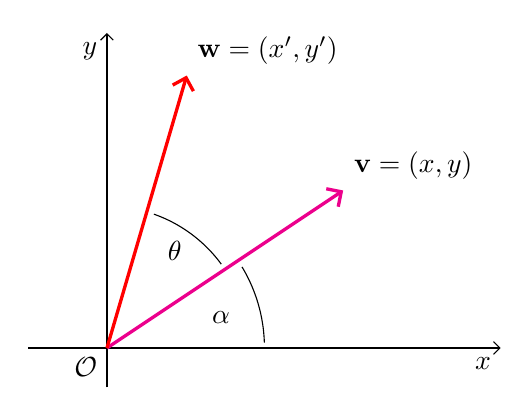
\begin{tikzpicture}[% styles used in image code
         > = Straight Barb, % defined in "arrows.meta
dot/.style = {circle, fill,
              minimum size=2mm, inner sep=0pt, outer sep=0pt,
              node contents={}},
box/.style = {draw, thin, minimum  width=2mm, minimum height=4mm,
              inner sep=0pt, outer sep=0pt,
              node contents={}, sloped},
my angle/.style args = {#1/#2}{draw,->,
                               angle radius=#1,
                               angle eccentricity=#2,
                               } % angle label position!
                        ]
	% coordinate axis
	\draw[->] (-1, 0)   -- (5,0) node[below left] {$x$};
	\draw[->] ( 0,-0.5) -- (0,4) node[below left] {$y$};

	\coordinate (O) at (0,0);
	\coordinate (v1) at (3,2);
	\coordinate (v2) at (1.013,3.460);
	
	\draw (O) node[below left] {$\mathcal{O}$};
	\draw [->,magenta,very thick] (O) --(v1) node[above right,black] {$\mathbf{v}=(x,y)$};
	\draw [->,red,very thick] (O) --(v2) node[above right,black] {$\mathbf{w}=(x',y')$};
	
	\begin{scope}
	\path[clip] (O) -- (3,0.1) -- ($(v1)+(0,-0.2)$);
	\draw[black] (O) circle (20mm);
	\node at ($(O)+(15:15mm)$) {$\alpha$};
	\end{scope}
	
	\begin{scope}
	\path[clip] (O) -- ($(v1)+(0,0.2)$) -- ($(v2)+(0.2,0)$);
	\draw[black] (O) circle (18mm);
	\node at ($(O)+(55:15mm)$) {$\theta$};
	\end{scope}
\end{tikzpicture} \caption*{Rotation of Euclidean vectors.}
\end{figure}

\noindent The rotated vector has a decomposition with its norm and angle as
\begin{align*}
x' &= \|\mathbf{w}\| \cos(\alpha+\theta)\\
y' &= \|\mathbf{w}\| \sin(\alpha+\theta)
\end{align*}
Rotation doesn't change the norm of a vector, so $\|\mathbf{w}\| = \|\mathbf{v}\| = \sqrt{x^2+y^2}$. Then, using the angle sum trigonometry identities we have
\begin{align*}
&\begin{array}{l}
x' = \sqrt{x^2+y^2} \left( \cos\alpha\cos\theta-\sin\alpha\sin\theta \right)\\
y' = \sqrt{x^2+y^2} \left( \sin\alpha\cos\theta + \cos\alpha\sin\theta \right)
\end{array} \\ \\
\implies
& \begin{array}{l}
x' = \sqrt{x^2+y^2} \left( \dfrac{x}{\sqrt{x^2+y^2}}\cos\theta-\dfrac{y}{\sqrt{x^2+y^2}}\sin\theta \right)\\
y' = \sqrt{x^2+y^2} \left( \dfrac{y}{\sqrt{x^2+y^2}}\cos\theta + \dfrac{x}{\sqrt{x^2+y^2}}\sin\theta \right)
\end{array} \\ \\
\implies
& \begin{array}{l}
x' = x\cos\theta-y\sin\theta \\
y' = y\cos\theta + x\sin\theta 
\end{array}
\end{align*}
We can represent the rotated vector as the column
\begin{align*}
\begin{pmatrix} x' \\ y' \end{pmatrix}
=
\begin{pmatrix} 
x\cos\theta - y\sin\theta \\ 
x\sin\theta + y\cos\theta 
\end{pmatrix}
=
\begin{pmatrix} 
x\cos\theta \\ 
x\sin\theta
\end{pmatrix}
+
\begin{pmatrix} 
- y\sin\theta \\ 
y\cos\theta 
\end{pmatrix}
=
x
\begin{pmatrix} 
\cos\theta \\ 
\sin\theta
\end{pmatrix}
+
y
\begin{pmatrix} 
- \sin\theta \\ 
\cos\theta 
\end{pmatrix}
\end{align*}
This last expression is how we've defined a matrix multiplied by a column! So we have
\begin{gather*}
\begin{pmatrix} x' \\ y' \end{pmatrix}
=
\begin{pmatrix} 
\cos\theta & -\sin\theta \\ 
\sin\theta &  \cos\theta  
\end{pmatrix}
\begin{pmatrix} x \\ y \end{pmatrix}
\end{gather*}
which gives us the definition of the general rotation matrix:

\definition{Rotation matrix - arbtirary angle anti-clockwise}{
By using a column $X\in\mathcal{M}_{2,1}$ to represent a Euclidean vector, the following matrix allows the operation of rotataion, anti-clockwise, of $X$ by an angle $\theta$:
\begin{align*}
R_\theta =
\begin{pmatrix} 
\cos\theta & -\sin\theta \\ 
\sin\theta &  \cos\theta  
\end{pmatrix}
\end{align*}
where the rotated vector is represented by a column $X'\in\mathcal{M}_{2,1}$ obtained by matrix multiplication $X' = R_\theta X$.
}

\subsection*{Reflection matrices}

\subsection*{Compression and dilation matrices}

\subsection*{Skew matrices}

\subsection*{Summary of Euclidean transformation matrices}

\begin{table}[H]
\begin{center}
\begin{tabular}{l|l}
Transformation & Matrix \\ \hline\hline \\[-7pt]
Rotation by 45 degrees & $R_{\theta=\pi/4} = \dfrac{1}{\sqrt{2}}\begin{pmatrix} 1 & -1 \\ 1 & 1 \end{pmatrix}$ \\[10pt] \hline  \\[-7pt]
Rotation by 90 degrees & $R_{\theta=\pi/2} = \begin{pmatrix} 0 & -1 \\ 1 & 0 \end{pmatrix}$ \\[10pt] \hline \\[-7pt]
Rotation by $\theta$ degrees & $R_{\theta} = \begin{pmatrix} \cos\theta & -\sin\theta \\ \sin\theta & \cos\theta \end{pmatrix}$ \\[10pt] \hline \\[-7pt]
Reflection across $x$-axis & $R_{x} = \begin{pmatrix} 1 & 0 \\ 0 & -1 \end{pmatrix}$ \\ [10pt] \hline \\[-7pt]
Reflection across $y$-axis & $R_{y} = \begin{pmatrix} -1 & 0 \\ 0 & 1 \end{pmatrix}$ \\ [10pt] \hline \\[-7pt]
Reflection across $y=x$ line & $R_{y=x} = \begin{pmatrix} 0 & 1 \\ 1 & 0 \end{pmatrix}$ \\ [10pt] \hline \\[-7pt]
Reflection across $y=-x$ line & $R_{y=-x} = \begin{pmatrix} 0 & -1 \\ -1 & 0 \end{pmatrix}$ \\[10pt] \hline \\[-7pt]
Reflection across origin & $R_{\mathcal{O}} = \begin{pmatrix} -1 & 0 \\ 0 & -1 \end{pmatrix}$ \\[10pt] \hline \\[-7pt]
Dilation & $D = \begin{pmatrix} k & 0 \\ 0 & k \end{pmatrix}, \quad k>1$ \\[10pt] \hline \\[-7pt]
Compression & $D = \begin{pmatrix} k & 0 \\ 0 & k \end{pmatrix}, \quad 0\leq k<1$ \\[10pt] \hline \\[-7pt]
Skew in the $x$ direction & $S_{x,k} = \begin{pmatrix} k & 0 \\ 0 & 1 \end{pmatrix}$ \\[10pt] \hline \\[-7pt]
Skew in the $y$ direction & $S_{y,k} = \begin{pmatrix} 1 & 0 \\ 0 & k \end{pmatrix}$
\end{tabular}
\end{center}
\end{table}

\section{Multiplication of matrices by matrices}

We will start with the definition of matrix multiplication before justifying some of its properties.

\definition{Multiplication of two matrices}{
Consider two matrices $A \in \mathcal{M}_{n,m}$ and $B \in \mathcal{M}_{m,q}$. We define the product $AB$ to be the matrix $C\in\mathcal{M}_{n,q}$ with coefficients
\begin{gather*}
c_{ij} = a_{i1}b_{1j} + a_{i2}b_{2j} + \cdots + a_{im}b_{mj} = \sum_{k=1}^m a_{ik} b_{kj} \\
%%%
%%%
%%%
\implies
\begin{pmatrix}
a_{11} & a_{12} & \cdots & a_{1m} \\
a_{21} & a_{22} & \cdots & a_{2m} \\
\vdots & \vdots & \ddots & \vdots \\
a_{n1} & a_{n2} & \cdots & a_{nm}
\end{pmatrix}
\begin{pmatrix}
b_{11} & b_{12} & \cdots & b_{1q} \\
b_{21} & b_{22} & \cdots & b_{2q} \\
\vdots & \vdots & \ddots & \vdots \\
b_{m1} & b_{m2} & \cdots & b_{mq}
\end{pmatrix} \\
%%%
%%%
%%%
=
\left(
b_{11}
\underbrace{
\begin{pmatrix}
a_{11} \\
a_{21} \\
\vdots \\
a_{n1} 
\end{pmatrix}
+ \cdots +
b_{m1}
\begin{pmatrix}
a_{1m} \\
a_{2m} \\
\vdots \\
a_{nm} 
\end{pmatrix}
}_{\text{\large first column}}
%%
\quad \cdots \quad 
%%
b_{1q}
\underbrace{
\begin{pmatrix}
a_{11} \\
a_{21} \\
\vdots \\
a_{n1} 
\end{pmatrix}
+ \cdots +
b_{mq}
\begin{pmatrix}
a_{1m} \\
a_{2m} \\
\vdots \\
a_{nm} 
\end{pmatrix}
}_{\text{\large n$^{th}$ column}}
\right)
\end{gather*}
Additionally, for the product
\begin{align*}
\underbrace{A}_{(\colorbox{Mahogany!20}{n},\colorbox{airforceblue!20}{m})} \underbrace{B}_{(\colorbox{airforceblue!20}{m},\colorbox{Mahogany!20}{q})}
\end{align*}
we will call the indices for the columns of $A$ and rows of $B$ the \textit{inner indices} (blue), whereas the indices for the rows of $A$ and columns of $B$ will be called the \textit{outer indices} (red).
}

\example{Matrix multiplication}{
\begin{align*}
\begin{pmatrix}
      1 &  2 & 4  \\
      3 & -1 & 0  \\
\end{pmatrix}
\begin{pmatrix}
      2 &  5  \\
      1 &  3  \\
     -1 & -4  \\
\end{pmatrix}
=
\left(
\overbrace{
2\begin{pmatrix}
1 \\
3
\end{pmatrix}
+
1\begin{pmatrix}
2 \\
-1
\end{pmatrix}
-1\begin{pmatrix}
4 \\
0
\end{pmatrix}
}^{\text{\large first column}}
%%%
\quad
%%%
\overbrace{
5\begin{pmatrix}
1 \\
3
\end{pmatrix}
+
3\begin{pmatrix}
2 \\
-1
\end{pmatrix}
-4\begin{pmatrix}
4 \\
0
\end{pmatrix}
}^{\text{\large second column}}
\right)
=
\begin{pmatrix}
 0 & -5 \\
 5 & 12
\end{pmatrix}
\end{align*}
}

\noindent It should be clear that the j$^{th}$ column of the result is like we just did matrix multiplication of $A$ by the j$^{th}$ column of $B$. Otherwise put, the i,j$^{th}$ element of $AB$ comes from the dot product of the i$^{th}$ row of $A$ by the j$^{th}$ column of $B$: $c_{ij}=(a_{i1}, a_{i2}, \dots , a_{im})\cdot(b_{1j},b_{2j},\dots,b_{mj})=\mathbf{A_{(i)}}\cdot\mathbf{B^{(j)}}$. Visually:
\begin{align*}
&
\begin{pmatrix}
a_{11} & a_{12} & \cdots & a_{1m} \\
a_{21} & a_{22} & \cdots & a_{2m} \\
\vdots & \vdots & \ddots & \vdots \\
a_{n1} & a_{n2} & \cdots & a_{nm}
\end{pmatrix}
\begin{pmatrix}
b_{11} & b_{12} & \cdots & b_{1q} \\
b_{21} & b_{22} & \cdots & b_{2q} \\
\vdots & \vdots & \ddots & \vdots \\
b_{m1} & b_{m2} & \cdots & b_{mq}
\end{pmatrix} \\
&=
\begin{pmatrix}
\mathbf{A}_{(1)}\cdot\mathbf{B}^{(1)} & \mathbf{A}_{(1)}\cdot\mathbf{B}^{(2)} & \cdots & \mathbf{A}_{(1)}\cdot\mathbf{B}^{(m)} \\
\mathbf{A}_{(2)}\cdot\mathbf{B}^{(1)} & \mathbf{A}_{(2)}\cdot\mathbf{B}^{(2)} & \cdots & \mathbf{A}_{(2)}\cdot\mathbf{B}^{(m)} \\
\vdots & \vdots & \ddots & \vdots \\
\mathbf{A}_{(n)}\cdot\mathbf{B}^{(1)} & \mathbf{A}_{n}\cdot\mathbf{B}^{(2)} & \cdots & \mathbf{A}_{(n)}\cdot\mathbf{B}^{(m)}
\end{pmatrix}
\end{align*}



\example{Matrix multiplication with dot products}{
\begin{align*}
\begin{pmatrix}
      3 &  0 \\
     -1 &  2
\end{pmatrix}
\begin{pmatrix}
      1 &  2 & -4  \\
      1 & -3 &  1
\end{pmatrix}
&=
\begin{pmatrix}
  \mathbf{A}_{(1)}\cdot\mathbf{B}^{(1)} & \mathbf{A}_{(1)}\cdot\mathbf{B}^{(2)}  & \mathbf{A}_{(1)}\cdot\mathbf{B}^{(3)}  \\
  \mathbf{A}_{(2)}\cdot\mathbf{B}^{(1)}  & \mathbf{A}_{(2)}\cdot\mathbf{B}^{(2)} &  \mathbf{A}_{(2)}\cdot\mathbf{B}^{(3)}
\end{pmatrix}
%%%%
%%%%
%%%%
\\
&=
\begin{pmatrix}
  (3,0)\cdot(1,1) & (3,0)\cdot(2,-3)  & (3,0)\cdot(-4,1)  \\
  (-1,2)\cdot(1,1) & (-1,2)\cdot(2,-3)  & (-1,2)\cdot(-4,1)
\end{pmatrix} 
\\
&=
\begin{pmatrix}
  3 &  6  & -12  \\
  1 & -8  &   6
\end{pmatrix}
\end{align*}
}

Let's now try to understand why the shapes must be what they are. Suppose we have two matrices $A$ and $B$. We would like to define the matrix multiplication $AB=C$ so that the following associative law holds:
\begin{align*}
CX = (AB)X = A(BX)
\end{align*}
for a column $X$ of an appropriate size. 

Let's start with $B$ as the matrix with known size $m \times n$. This forces the size of $X$ \textit{given how we defined multiplication of a matrix by a column}: $X$ must have the same number of elements as \textit{columns} of $B$. So $X\in\mathcal{M}_{n,1}$ and the multiplication $BX$ gives a new column $X'$ with known shape: 
\begin{align*}
\underbrace{B}_{(m,n)} \underbrace{X}_{(n,1)} = \underbrace{X'}_{(m,1)}
\end{align*}
So $A(BX)$ becomes $AX'$, another multiplication of a matrix by a column. So $A$ must have the same number of columns as the elements of the column it multiplies: $A\in\mathcal{M}_{q,n}$ for some $q$. The multiplication $AX'$ gives a new column $X''$ with known shape: 
\begin{align*}
\underbrace{A}_{(q,n)} \underbrace{X'}_{(n,1)} = \underbrace{X''}_{(q,1)}
\end{align*}
Finally we have $CX = X''$. This forces the shape of $C$, the product of $A$ and $B$. $C$ must have the same number of columns as elements of $X$, $n$. The column $X''$ must have the same number of elements, $q$, as \textit{rows} of $C$. So we have $C\in\mathcal{M}_{q,n}$. Notice that this means the shape of the product $A$ and $B$ comes from the outer indices of their shapes:
\begin{align*}
\underbrace{A}_{(\colorbox{Mahogany!20}{n},\colorbox{airforceblue!20}{m})} \underbrace{B}_{(\colorbox{airforceblue!20}{m},\colorbox{ForestGreen!30}{q})} = \underbrace{C}_{(\colorbox{Mahogany!20}{n},\colorbox{ForestGreen!30}{q})}
\end{align*}
The inner indices must be the same, $m$ in this case, and doesn't appear in the answer.




\example{Multiplication of rotation matrices}{
Let $R_\theta$ and $R_\phi$ be anti-clockwise rotation matrices for angles $\theta$ and $\phi$. That is
\begin{align*}
R_\theta
=
\begin{pmatrix} \cos\theta & -\sin\theta \\ \sin\theta & \cos\theta \end{pmatrix}
\quad \text{and} \quad
R_\alpha
=
\begin{pmatrix} \cos\phi & -\sin\phi \\ \sin\phi & \cos\phi \end{pmatrix}
\end{align*}
When we multiply these matrices we get
\begin{align*}
R_\theta R_\alpha
&=
\begin{pmatrix} \cos\theta & -\sin\theta \\ \sin\theta & \cos\theta \end{pmatrix}
\begin{pmatrix} \cos\phi & -\sin\phi \\ \sin\phi & \cos\phi \end{pmatrix} \\
&=
\begin{pmatrix}
\cos\theta\cos\phi - \sin\theta\sin\phi & -\cos\theta\sin\phi -\sin\theta\cos\phi \\
\sin\theta\cos\phi + \cos\theta\sin\phi & -\sin\theta\sin\phi +\cos\theta\cos\phi
\end{pmatrix} \\
&=
\begin{pmatrix}
\cos(\theta+\phi) & -\sin(\theta+\phi) \\
\sin(\theta+\phi) & \cos(\theta+\phi)
\end{pmatrix}
\end{align*}
This result is just an anti-clockwise rotation matrix for angle $\theta+\phi$. This should make sense. Rotating a vector by $\theta$, and then rotating the resulting vector by $\phi$ is the same as doing it in one go by the addition of these angles.
}

\theorem{Square matrix multiplication and commutativity}{
For any two matrices $A$ and $B$, if the products $AB$ and $BA$ are well defined then both products result in square matrices. If the products give the same result, $AB=BA$, then both $A$ and $B$ must also be square matrices of the same shape.
}
\begin{proof}
Let $A\in\mathcal{M}_{m,n}$ and $B\in\mathcal{M}_{p,q}$. Then for $AB$ to be well defined, recall that the inner indices must be equal: the number of columns of $A$ must match the number of rows of $B$, so $n=p$. Similarly for $BA$ to be well defined, the number of columns of $B$ must match the number of rows of $A$, so $q=m$. Hence $B\in\mathcal{M}_{n,m}$ and therefore
\begin{itemize}
\item $AB \in\mathcal{M}_{m,m}$, and
\item $BA \in\mathcal{M}_{n,n}$.
\end{itemize}
Now if we have that $AB=BA$ we must have that $m=n$. Hence
\begin{itemize}
\item $A \in\mathcal{M}_{m,n}=\mathcal{M}_{m,m}$, and
\item $B \in\mathcal{M}_{p,q}=\mathcal{M}_{n,m}=\mathcal{M}_{m,m}$.
\end{itemize}

\end{proof}

\noindent Now that multiplication of matrices is well defined, we can introduce the notion of the multiplicative identity, the parallel of the number 1 for matrices. That is, the identity matrix $I$ should multiply by any matrix, say $A$, and return the same: $IA=A$. Suppose $A\in\mathcal{M}_{m,n}$ and $I\in\mathcal{M}_{p,q}$, so we have
\begin{align*}
\underbrace{I}_{(p,q)} \underbrace{A}_{(m,n)} = \underbrace{A}_{(m,n)}.
\end{align*}
Then to satisfy the shapes condition we must have that the inner indices match, so $q=m$, and outer indices give the resulting shape, so $p=m$. So $I$ must be a square matrix $I\in\mathcal{M}_{m,m}$ where the size matches the number of rows of $A$. Now we can look at each element in the product
\begin{align*}
(IA)_{ij} &= \mathbf{I}_{(i)}\cdot\mathbf{A}^{(j)} \\
&= (I)_{i1}a_{1j} + (I)_{i2}a_{2j} + \cdots + (I)_{ii}a_{ij} + \cdots + (I)_{im}a_{mj}.
\end{align*}
This must equal $a_{ij}$ to satisfy $IA=A$ and so $(I)_{ik}=0$ for all the $k$ except $k=i$ where $(I)_{ii}=1$. So we have the following definition.

\definition{Identity matrix}{
The $n$-dimensional identity matrix $I$ is a square matrix of size $n\times n$ with 1s along the diagonal and 0s elsewhere, that is, 
\begin{align*}
(I)_{ij}
=
\begin{cases}
1 & \text{whenever } \, i=j, \\
0 & \text{whenever } \, i \neq j.
\end{cases}
\end{align*}
}

\example{Identity matrices}{
\begin{align*}
I_2 =
\begin{pmatrix}
1 & 0 \\
0 & 1
\end{pmatrix}
\quad\quad
I_3 =
\begin{pmatrix}
1 & 0 & 0 \\
0 & 1 & 0 \\
0 & 0 & 1
\end{pmatrix}
\end{align*}
}

We have defined above, in fact, the \textit{left} identity matrix because the defining relation was multiplication on the left $IA=A$. If we have $AI=A$ then by the previous reasoning we find $I$ must be a square matrix with size matching the columns of $A$ instead. It's only in the case that $A$ itself is a square matrix that we can have a two-sided identity matrix satisfying $IA=AI=A$.

\example{Matrix multiplication giving the zero matrix}{
Curiously, we can have two non-zero matrices multiply to give a zero matrix:
\begin{gather*}
\begin{pmatrix}
1 & 2 \\
0 & 0
\end{pmatrix}
\begin{pmatrix}
0 & 3 \\
0 & 2
\end{pmatrix}
=
\begin{pmatrix}
0 & 0 \\
0 & 0
\end{pmatrix}
\\
\begin{pmatrix}
1 & 2 & 0 \\
1 & 0 & -1
\end{pmatrix}
\begin{pmatrix}
0 &  2 \\
0 & -1 \\
0 &  2
\end{pmatrix}
=
\begin{pmatrix}
0 & 0 \\
0 & 0
\end{pmatrix}
\end{gather*}
}


Just like the zero matrix gives us the idea of the additive inverse, the identity matrix gives the idea of the \textit{multiplicative} inverse. However, though every matrix has an additive inverse, not every matrix will have a multiplicative inverse. The following gives the defining relation of invertible matrices.

\definition{Invertible matrix}{
A matrix $A$ is invertible if and only if there exists a matrix $B$ such that
\begin{align*}
A B = BA = I
\end{align*}
This matrix $B$ is called the inverse of $A$ and is denoted $A^{-1}$. As we have commutative matrices, $AB=BA$, recall that this can only happen if $A$ is square. So, only square matrices can have inverses.
}

\example{Invertible matrix}{
Let $A=\begin{pmatrix} 1 & 2 \\ 0 & -1 \end{pmatrix}$. Given that
\begin{align*}
\begin{pmatrix} 1 & 2 \\ 3 & -1 \end{pmatrix}
\begin{pmatrix} 1/7 & 2/7 \\ 3/7 & -1/7 \end{pmatrix}
=
\begin{pmatrix} 1 & 0 \\ 0 & 1 \end{pmatrix},
\end{align*}
then we have $A^{-1}=\begin{pmatrix} 1/7 & 2/7 \\ 3/7 & -1/7 \end{pmatrix}$.
}

\noindent Before we develop techniques for finding inverses of matrices, we will introduce a function that allows us to determine \textit{whether} a given square matrix is invertible or not. This function is called the determinant. 

\section{Determinants of matrices}

The idea of the determinant of a matrix is to assign a single number to any square matrix which can be used to determine if that matrix is invertible or not. It will turn out that the determinant of a matrix will break down into determinants of smaller matrices. So we start with determinants of 1 by 1 matrices.

Suppose we have a general 1 by 1 matrix $A = \begin{pmatrix} a \end{pmatrix}$. It shouldn't be too difficult to see that the inverse matrix must be $A^{-1} = \begin{pmatrix} 1/a \end{pmatrix}$ because the multiplication $\begin{pmatrix} a \end{pmatrix}\begin{pmatrix} 1/a \end{pmatrix} = \begin{pmatrix} 1 \end{pmatrix}$, the identity matrix. Since $1/a$ is well defined only if $a\neq 0$, the value of $a$ itself satisfies this idea ``if this value is non-zero, the matrix is invertible''. So we have justified the following.

\definition{Determinant of a 1 by 1 matrix}{
The determinant of any 1 by 1 matrix is given by its only coefficient:

\begin{align*}
\det \left( \begin{pmatrix} a \end{pmatrix}\right)  = a
\end{align*}
}

Now, to define the determinant of any matrix, as stated before there is an iterative process where the determinant of an $n\times n$ matrix is equal to a certain combination of determinants of $n-1 \times n-1$ matrices. So we first have to define how to break apart a matrix into particular smaller \textit{submatrices}.

\definition{Submatrix}{
From a matrix $A$ we generate the \textit{submatrix} $A_{ij}$ by deleting the $ith$ row and $jth$ column:
\begin{align*}
\text{For} \, A =
\begin{pmatrix}
a_{1,1}   & \cdots & a_{1,j-1}   & a_{1,j}   & a_{1,j+1}   & \cdots & a_{1,n}   \\
\vdots    & \cdots & \vdots      & \vdots    & \vdots      & \cdots & \vdots    \\
a_{i-1,1} & \cdots & a_{i-1,j-1} & a_{i-1,j} & a_{i-1,j+1} & \cdots & a_{i-1,n} \\
a_{i,1}   & \cdots & a_{i,j-1}   & a_{i,j}   & a_{i,j+1}   & \cdots & a_{i,n}   \\
a_{i+1,1} & \cdots & a_{i+1,j-1} & a_{i+1,j} & a_{i+1,j+1} & \cdots & a_{i+1,n} \\
\vdots    & \cdots & \vdots      & \vdots    & \vdots      & \cdots & \vdots    \\
a_{m,1}   & \cdots & a_{m,j-1}   & a_{m,j}   & a_{m,j+1}   & \cdots & a_{m,n} 
\end{pmatrix} \\
\text{The submatrix} \, A_{ij} =
\begin{pmatrix}
a_{1,1}   & \cdots & a_{1,j-1}   & a_{1,j+1}   & \cdots & a_{1,n}   \\
\vdots    & \cdots & \vdots      & \vdots      & \cdots & \vdots    \\
a_{i-1,1} & \cdots & a_{i-1,j-1} & a_{i-1,j+1} & \cdots & a_{i-1,n} \\
a_{i+1,1} & \cdots & a_{i+1,j-1} & a_{i+1,j+1} & \cdots & a_{i+1,n} \\
\vdots    & \cdots & \vdots      & \vdots      & \cdots & \vdots    \\
a_{m,1}   & \cdots & a_{m,j-1}   & a_{m,j+1}   & \cdots & a_{m,n} 
\end{pmatrix}
\end{align*}
\textit{Note}: we generally have to specify in words that we create a submatrix. The notation $A_{ij}$ is a little ambiguous without being explicit. 
}


\example{Submatrices of a $3\times 3$ matrix}{
Let $A = 
\begin{pmatrix}
  1 &  0 &  3 \\
 -1 &  2 & -1 \\
  2 & -3 &  0
\end{pmatrix},$ then some submatrices of $A$ are
\begin{align*}
A_{13}
=
\begin{pmatrix}
 -1 &  2 \\
  2 & -3
\end{pmatrix},
\qquad
A_{22}
=
\begin{pmatrix}
  1 &  3 \\
  2 &  0
\end{pmatrix},
\qquad
A_{32}
=
\begin{pmatrix}
  1 &  3 \\
 -1 & -1
\end{pmatrix}.
\end{align*}
}

\noindent Now we are ready to define the general determinant operation.

\definition{Determinant of an $n \times n$ matrix}{
For any square matrix $A\in\mathcal{M}_{n,n}$, its determinant is given by
\begin{align*}
\det(A) = \sum_{i=1}^n (-1)^{i+j} a_{ij} \det(A_{ij})
\end{align*}
where the $a_{ij}$ are coefficients of $A$, $A_{ij}$ is the $i,j^{th}$ submatrix of $A$ and for any $1\leq j \leq n$. We can also sum over the $j$ index for any $1\leq i \leq n$
\begin{align*}
\det(A) = \sum_{j=1}^n (-1)^{i+j} a_{ij} \det(A_{ij})
\end{align*}
and we will show that the answer is the same.
}

\noindent This definition hides what is in fact a fairly simple computation that becomes very clear with some examples. Suppose we have a general 2 by 2 matrix 
\begin{align*}
A = \begin{pmatrix} a & b \\ c & d\end{pmatrix}
\end{align*}
The determinant is therefore (choosing $j=1$ for the first summation)
\begin{align*}
\det(A) = \sum_{i=1}^n (-1)^{i+1} a_{i1} \det(A_{i1}) &= (-1)^{2} a_{11} \det(A_{11}) + (-1)^{3} a_{21} \det(A_{21})\\
 &= a \det\begin{pmatrix} d\end{pmatrix} - c \det\begin{pmatrix} b \end{pmatrix}.
\end{align*}
We defined earlier the determinants of 1 by 1 matrices, so we have the following formula worth remembering.

\theorem{Determinant of a $2\times 2$ matrix}{
For a $2\times 2$ matrix
\begin{align*}
A =
\begin{pmatrix}
a & b \\
c & d
\end{pmatrix}
\end{align*}
its determinant, denoted $\det(A)$ or $|A|$, is given by
\begin{align*}
\det \begin{pmatrix}
a & b \\
c & d
\end{pmatrix}
=
\left|
\begin{matrix}
a & b \\
c & d
\end{matrix}
\right|
= ad - bc
\end{align*}
}

\noindent This function will be used so often it's worth memorising it. I remember its form by saying in my head ``on-diagonal minus off-diagonal'', where ``on-diagonal'' means the multiplication of the diagonal terms, $a$ and $d$, and ``off-diagonal'' means the multiplication of the other terms, $b$ and $c$.

\example{Determinant of a 3 by 3 matrix}{
Let $A = 
\begin{pmatrix}
  1 &  0 &  3 \\
 -1 &  2 & -1 \\
  2 & -3 &  0
\end{pmatrix}$. If we choose $j=2$, we are ``summing down column 2'':
\begin{align*}
\left|
\begin{matrix}
  1 &  \colorbox{Mahogany!30}{0} &  3 \\
 -1 &  \colorbox{ForestGreen!30}{2} & -1 \\
  2 & \colorbox{airforceblue!30}{-3} &  0
\end{matrix}
\right|
&= 
(-1)^{1+2}\colorbox{Mahogany!30}{0}|A_{12}| + (-1)^{2+2}\colorbox{ForestGreen!30}{2}|A_{22}| + (-1)^{3+2}\colorbox{airforceblue!30}{($-$3)}|A_{32}|
\\
&=
-\colorbox{Mahogany!30}{0}
\left|\begin{matrix}
 -1 &  -1 \\
  2 &  0
\end{matrix}\right|
+
\colorbox{ForestGreen!30}{2}
\left|\begin{matrix}
  1 &  3 \\
  2 &  0
\end{matrix}\right|
+
-\colorbox{airforceblue!30}{$-$3}
\left|\begin{matrix}
  1 &   3 \\
 -1 &  -1 \\
\end{matrix}\right|
\\
&=
\colorbox{ForestGreen!30}{2}
\left((1)(0) - (3)(2)\right)
+
\colorbox{airforceblue!30}{3}
\left((1)(-1) - (3)(-1)\right)
\\ 
&=
\colorbox{ForestGreen!30}{2}\times -6
+
\colorbox{airforceblue!30}{3}\times 2 
\\
&= -6
\end{align*}

If instead we choose $i=1$, then we are ``summing across row 1'':
\begin{align*}
\left|
\begin{matrix}
  \colorbox{Mahogany!30}{1} &  \colorbox{ForestGreen!30}{0} &  \colorbox{airforceblue!30}{3} \\
 -1 &  2 & -1 \\
  2 & -3 &  0
\end{matrix}
\right|
&= 
(-1)^{1+1}\colorbox{Mahogany!30}{1}|A_{11}| + (-1)^{2+1}\colorbox{ForestGreen!30}{0}|A_{12}| + (-1)^{3+1}\colorbox{airforceblue!30}{3}|A_{13}|
\\
&=
\colorbox{Mahogany!30}{1}
\left|\begin{matrix}
 2 & -1 \\
 -3 &  0
\end{matrix}\right|
-
\colorbox{ForestGreen!30}{0}
\left|\begin{matrix}
 -1 & -1 \\
  2 &  0
\end{matrix}\right|
+
\colorbox{airforceblue!30}{3}
\left|\begin{matrix}
 -1 &  2 \\
  2 & -3 
\end{matrix}\right|
\\
&=
\colorbox{Mahogany!30}{1}
\left((2)(0) - (-1)(-3)\right)
-
\colorbox{ForestGreen!30}{0}
\left((-1)(0) - (-1)(2)\right)
+
\colorbox{airforceblue!30}{3}
\left((-1)(-3) - (2)(2)\right)
\\ 
&=
\colorbox{Mahogany!30}{1}\times -3
+
\colorbox{airforceblue!30}{3}\times -1 
\\
&= -6
\end{align*}
Notice that we got the same answer in both cases.
}


\noindent In the determinant expression there is this term $(-1)^{i+j}$ that appears in both summations. It can only give two possible values:
\begin{align*}
(-1)^{i+j} = 
\begin{cases}
+1 & \text{if $i+j$ is even} \\
-1 & \text{if $i+j$ is odd}
\end{cases}
\end{align*}
As the $i$ and $j$ are the row and columns indices, respectivel, this term determines the following $+$ or $-$ pattern to any matrix
\begin{align*}
\begin{pmatrix}
+ & - & + & - & \cdots \\
- & + & - & + & \cdots \\
+ & - & + & - & \cdots \\
\vdots & \vdots & \vdots & \vdots & \ddots
\end{pmatrix}
\end{align*}
Noticing this pattern lets you avoid having to explicitly write $(-1)^{i+j}$ during the calculations.

\theorem{Determinant when a column is multiplied by a constant}{
If we multiply a column by a constant, $k$, then the determinant is multiplied by that constant. 
\vspace{-0.1cm}\begin{center} \textcolor{airforceblue}{\rule{0.7\textwidth}{0.3mm}} \end{center}
}

\begin{proof} Let's multiply the j$^{th}$ column of a matrix $A$ by $k$ to get the new matrix
\begin{align*}
A' =
\begin{pmatrix}
a_{11} & \cdots & ka_{1j} & \cdots & a_{1n} \\
a_{21} & \cdots & ka_{2j} & \cdots & a_{2n} \\
\vdots & \ddots & \vdots & \cdots & \vdots \\
a_{n1} & \cdots & ka_{nj} & \cdots & a_{nn}
\end{pmatrix}
\end{align*}
Then, calculate the determinant of $A'$, choosing to compute it along the j$^{th}$ column
\begin{align*}
\det(A') = \sum_{i=1}^n (-1)^{i+j} (ka_{ij}) \det(A'_{ij}) = k\sum_{i=1}^n (-1)^{i+j} a_{ij} \det(A'_{ij}) = k \det (A)
\end{align*}
\end{proof}

\theorem{Determinant of a multiplication}{
Given two matrices $A,B\in \mathcal{M}_{n,n}$, we have
\begin{align*}
\det(AB)=\det(A)\det(B)
\end{align*}
}

\theorem{Determinant of a diagonal matrix}{
Let $A\in\mathcal{M}_{n,n}$ be a diagonal matrix. Then
\begin{align*}
\det(A)=a_{11}\times a_{22} \times \cdots \times a_{nn}
\end{align*}
}

\theorem{Determinant of a triangular matrix}{
Let $A\in\mathcal{M}_{n,n}$ be a triangular matrix. Then
\begin{align*}
\det(A)=a_{11}\times a_{22} \times \cdots \times a_{nn}
\end{align*}
}

\begin{proof} Consider an upper triangular matrix
\begin{align*}
A =
\begin{pmatrix}
a_{11} & a_{12} & \cdots & a_{1n} \\
0 & a_{22} & \cdots & a_{2n} \\
\vdots & \vdots & \ddots & \vdots \\
0 & 0 & \cdots & a_{nn}
\end{pmatrix}
\end{align*}
If we take the determinant along the first column at each step we get
\begin{align*}
\det(A) 
= a_{11} 
\det\begin{pmatrix}
a_{22} & a_{23} & \cdots & a_{2n} \\
0 & a_{33} & \cdots & a_{3n} \\
\vdots & \vdots & \ddots & \vdots \\
0 & 0 & \cdots & a_{nn}
\end{pmatrix} 
= a_{11}a_{22} 
\det\begin{pmatrix}
a_{33} & a_{34} & \cdots & a_{3n} \\
0 & a_{44} & \cdots & a_{4n} \\
\vdots & \vdots & \ddots & \vdots \\
0 & 0 & \cdots & a_{nn}
\end{pmatrix}
= \cdots = a_{11}a_{22} \cdots  a_{nn}
\end{align*}
\end{proof}

\theorem{Determinant of any matrix multiplied by a diagonal matrix}{
Let $\Lambda, A\in\mathcal{M}_{n,n}$ with $\Lambda=\lambda I$ a diagonal matrix. Then
\begin{align*}
\det(\Lambda A)=\lambda^n \det(A)
\end{align*}
}

\theorem{Determinant of an inverse}{
Let $A\in\mathcal{M}_{n,n}$ be an invertible matrix. Then
\begin{align*}
\det(A) \neq 0 
\quad \text{and} \quad 
\det(A^{-1})=\frac{1}{\det(A)}
\end{align*}
}

\begin{proof} 
Since $A$ is invertible, its inverse exists and is defined by $AA^{-1}=I$. The determinant of this relation is
\begin{align*}
\det(AA^{-1}) &= \det(I) \\
\det(A)\det(A^{-1}) &= 1 \qquad (\implies \det(A^{-1})\neq 0 \text{ and } \det(A)\neq 0)\\
\det(A^{-1}) &=\frac{1}{\det(A)}
\end{align*}
\end{proof}

\theorem{Determinant of $PAP^{-1}$.}{
Let $P\in\mathcal{M}_{n,n}$ be an invertible matrix. Then for any matrix $A\in\mathcal{M}_{n,n}$ we have
\begin{align*}
\det(PAP^{-1}) = \det(A).
\end{align*}
}

\begin{proof} 
Using the ``determinant of a multiplication'' theorem we have
\begin{align*}
\det(PAP^{-1}) = \det(P)\det(A)\det(P^{-1}).
\end{align*}
These determinants are just numbers, so their multiplication is commutative:
\begin{align*}
\det(P)\det(A)\det(P^{-1}) &= \det(P)\det(P^{-1})\det(A) \\
 &= \det(P)\frac{1}{\det(P)}\det(A) \\
 &= \det(A)
\end{align*}
\end{proof}

\theorem{Determinant when two columns are equal}{
Let $A\in\mathcal{M}_{n,n}$ be a square matrix. If any two columns of $A$ are equal to each other then $\det(A)=0$.
}

For example
\begin{align*}
\det\begin{pmatrix}
 2 &  1 & 2 \\
 4 &  2 & 4 \\
 6 &  0 & 6 
\end{pmatrix}
=0.
\end{align*}

\theorem{Determinant when a column is a multiple of another}{
If any column is a multiple of another, then $\det(A)=0$.
}

For example
\begin{align*}
\det\begin{pmatrix}
 1 &  3 & 0 \\
 2 &  6 & 3 \\
 2 &  6 & 3 
\end{pmatrix}
=0.
\end{align*}



\theorem{Determinant and column exchange}{
Let $A\in\mathcal{M}_{n,n}$ be a square matrix. If we exchange any two columns, then the determinant of the new matrix is $-1$ times the old.
}

For example
\begin{align*}
\det\begin{pmatrix}
 2 &  1 & 7 \\
 4 &  2 & 4 \\
 6 &  0 & 3 
\end{pmatrix}
=-1
\det\begin{pmatrix}
 2 &  7 & 1 \\
 4 &  4 & 2 \\
 6 &  3 & 0 
\end{pmatrix}
\end{align*}

\theorem{Determinant and column operations}{
The determinant is unchanged if we add to a column a linear combination of other columns.
}

For example
\begin{align*}
\det\begin{pmatrix}
 2 &  1 & 7 \\
 4 &  2 & 4 \\
 6 &  0 & 3 
\end{pmatrix}
=
\det\begin{pmatrix}
 2 &  1 & 9 \\
 4 &  2 & 8 \\
 6 &  0 & 3 
\end{pmatrix}
\end{align*}
(the new third column is the old third column + 2 times the second column)


\theorem{Determinants and row properties and operations}{
For every square matrix $A$, the previous theorems about column properties and operations also hold for rows! That is, we have the following.
\begin{itemize}
\item If two rows are equal to each other, then $\det(A)=0$.
\item If any row is a multiple of another, then $\det(A)=0$.
\item If we exchange any two rows, the new determinant is $-1$ times the old.
\item The determinant is unchanged if we add to a row a linear combination of other rows.
\end{itemize}
}

\theorem{Existance of a triangular matrix with the same determinant}{
For every square matrix, $A$, there exists a triangular matrix, $T$, such that $\det(A)=\det(T)$.
}


\begin{proof}
Let $A$ be an $n$ by $n$ square matrix:
\begin{align*}
A =
\begin{pmatrix}
a_{11} & a_{12} & \cdots & a_{1n} \\
a_{21} & a_{22} & \cdots & a_{2n} \\
\vdots & \vdots & \ddots & \vdots \\
a_{n1} & a_{n2} & \cdots & a_{nn}
\end{pmatrix}
\end{align*}
Consider the first column. There are 2 possibilities:
\begin{enumerate}
\item All the $a_{i1}=0$. Then $\det(A)=0$ and the zero matrix is a triangular matrix with the same determinant.
\item There is a non-zero element in the first column, say $a_{k1}\neq 0$. We can add row $k$ to the first row, giving a new matrix $A'$ without changing the determinant. In this way we can always generate a matrix with a non-zero upper left element, $a'_{11}$, and the same determinant.
\end{enumerate}
Now we can use this $a'_{11}$ to guarantee it is the \textit{only} non-zero element in the first column. To do this we subtract from every row other than the first this particular multiple of the first row:
\begin{align*}
R_i \to R_i - \frac{a_{i1}}{a'_{11}}R_1
\end{align*}
This operation does not change the determinant, so we have:
\begin{align*}
\det(A)=\det\begin{pmatrix}
a'_{11} & a'_{12} & \cdots & a'_{1n} \\
a_{21} & a_{22} & \cdots & a_{2n} \\
\vdots & \vdots & \ddots & \vdots \\
a_{n1} & a_{n2} & \cdots & a_{nn}
\end{pmatrix}
=
\begin{pmatrix}
a'_{11} & a'_{12} & \cdots & a'_{1n} \\
0 & a^{(1)}_{22} & \cdots & a^{(1)}_{2n} \\
\vdots & \vdots & \ddots & \vdots \\
0 & a^{(1)}_{n2} & \cdots & a^{(1)}_{nn}
\end{pmatrix}
\end{align*}
We can repeat this procedure for the second column, ignoring the first row, to successively generate an upper triangular matrix
\begin{align*}
\det(A)=
\det\begin{pmatrix}
a'_{11} & a'_{12} & a'_{13} & \cdots & a'_{1n} \\
0 & a^{(1)}_{22} & a^{(1)}_{23} & \cdots & a^{(1)}_{2n} \\
0 & 0 & a^{(2)}_{33} & \cdots & a^{(2)}_{2n} \\
\vdots & \vdots & \vdots & \ddots & \vdots \\
0 & 0 & a^{(2)}_{3n} & \cdots & a^{(2)}_{nn}
\end{pmatrix}
=
\cdots
=
\det\begin{pmatrix}
a'_{11} & a'_{12} & a'_{13} & \cdots & a'_{1n} \\
0 & a^{(1)}_{22}  & a^{(1)}_{23} & \cdots & a^{(1)}_{2n} \\
0 & 0 & a^{(2)}_{33} & \cdots & a^{(2)}_{2n} \\
\vdots & \vdots & \vdots & \ddots & \vdots \\
0 & 0 & 0 & \cdots & a^{(n-1)}_{nn}
\end{pmatrix}
\end{align*}
and there's the triangular matrix.

\end{proof}

\noindent Now it's much easier to calculate the determinant of this triangular matrix (multiply the diagonal). In this way, at the end of the Gaussian reduction we can know immediately if the matrix is invertible or not (whether there is a zero on the diagonal).



\section{Matrix inversion}

Reminder: for a square matrix $M$, the inverse matrix $M^{-1}$ is defined by the relation:
\begin{align*}
M M^{-1} = M^{-1} M = I
\end{align*}
Where $I$ is the identity matrix of the same size as $M$. This inverse matrix is useful for solving systems of equations (with equal number of unknowns as equations). For example, for a system written in matrix form
\begin{align*}
AX = Y
\end{align*}
if the matrix $A$ has an inverse and we can compute it, then the unique solution to the
system is given by:
\begin{align*}
X = A^{-1}Y.
\end{align*}

Now, in the cofactor method of finding the inverse of a matrix we must introduce an associated matrix.

\definition{Cofactor matrix}{
From a matrix $A$ we generate its cofactor matrix $C_A$ which has entries given by determinants of submatrices of $A$ with the same plus/minus pattern as in a determinant calculation. That is, the entries of $C_A$ are $c_{ij}=(-1)^{i+j} \det(A_{ij})$:
\begin{align*}
C_A =
\begin{pmatrix}
 |A_{11}| & -|A_{12}| &  |A_{13}| & \cdots   \\
-|A_{21}| &  |A_{22}| & -|A_{23}| & \cdots   \\
 |A_{31}| & -|A_{32}| &  |A_{33}| & \cdots   \\
 \vdots   &  \vdots   &  \vdots   & \ddots
\end{pmatrix}
\end{align*}
}

With this cofactor matrix we can compute the inverse of any invertible square matrix.

\theorem{Inverse matrix (cofactor method)}{
The inverse of a matrix $A$ can be computed from its cofactor matrix:
\begin{align*}
A^{-1} = \frac{1}{\det(A)}C_A^T
\end{align*}
}

\example{Cofactor method}{
Let's use the cofactor method to find the inverse of the following matrix:
\begin{align*}
A = 
\begin{pmatrix}
  0 & 1 & -1 \\
  5 & 4 &  3 \\
  3 & 0 & -1
\end{pmatrix}
\end{align*}
First we need the determinant $\det(A)=26$ (verify this). Now there are nine elements to the comatrix:
\begin{align*}
C_{11} &= (-1)^{1+1}\left|\begin{matrix} 4 & 3 \\ 0 & -1 \end{matrix}\right|=-4, & 
C_{12} &= (-1)^{1+2}\left|\begin{matrix} 5 & 3 \\ 3 & -1 \end{matrix}\right|=14, & 
C_{13} &= (-1)^{1+3}\left|\begin{matrix} 5 & 4 \\ 3 & 0 \end{matrix}\right|=-12 \\
C_{21} &= (-1)^{2+1}\left|\begin{matrix} 1 & -1 \\ 0 & -1 \end{matrix}\right|=1,
&
C_{22} &= (-1)^{2+2}\left|\begin{matrix} 0 & -1 \\ 3 & -1 \end{matrix}\right|=3, &
C_{23} &= (-1)^{2+3}\left|\begin{matrix} 0 & 1 \\ 3 & 0 \end{matrix}\right|=3
\\
C_{31} &= (-1)^{3+1}\left|\begin{matrix} 1 & -1 \\ 4 & 3 \end{matrix}\right|=7,
&
C_{32} &= (-1)^{3+2}\left|\begin{matrix} 0 & -1 \\ 5 & 3 \end{matrix}\right|=-5, 
&
C_{33} &= (-1)^{3+3}\left|\begin{matrix} 0 & 1 \\ 5 & 4 \end{matrix}\right|=-5
\end{align*}
So we have the comatrix
\begin{align*}
C_A = 
\begin{pmatrix}
 -4 & 14 & -12 \\
  1 &  3 &   3 \\
  7 & -5 &  -5
\end{pmatrix}
\end{align*}
Transpose it, divide by the determinant of $A$ and we have the inverse of $A$
\begin{align*}
\begin{pmatrix}
  0 & 1 & -1 \\
  5 & 4 &  3 \\
  3 & 0 & -1
\end{pmatrix}^{-1}
=
\frac{1}{26}
\begin{pmatrix}
  -4 &  1 &  7 \\
  14 &  3 & -5 \\
 -12 &  3 & -5
\end{pmatrix}
\end{align*}
You should verify that $AA^{-1}=A^{-1}A=I$
}


\theorem{Inverse of a $2\times 2$ matrix}{
With the cofactor method, the inverse of a $2\times 2$ matrix is given by
\begin{align*}
\begin{pmatrix}
a & b \\
c & d
\end{pmatrix}^{-1}
=
\frac{1}{ad - bc}
\begin{pmatrix}
d & -c \\
-b & a
\end{pmatrix}
\end{align*}
}

%\chapter{Vector Spaces} \label{ch:vectorspaces}

\section{Introductory examples}

\subsection*{Set of polynomials of degree up to $n$}
Recall that the degree of a polynomial with variable $x$ is the power of the highest power of $x$ amongst all of the terms with non-zero coefficient. Let's consider all of the polynomials with degree up to and including $n$ with only real coefficients, denoted $P_n(\mathbb{R})$. An arbitrary member of this set can be written
\begin{align*}
\mathbf{p} = p_0 + p_1 x + p_2 x^2 + \cdots + p_n x^n = \sum_{i=0}^n p_i x^i
\end{align*}
where the coefficients $p_i \in \mathbb{R}$. Let's see what happens when we add another polynomial in the same set, say $\mathbf{q}\in P_n(\mathbb{R})$:
\begin{align*}
\mathbf{p} + \mathbf{q} &= \sum_{i=0}^n p_i x^i + \sum_{i=0}^n q_i x^i \\
&= \sum_{i=0}^n (p_i+ q_i) x^i \\
&= \mathbf{r}.
\end{align*}
We see the result is another polynomial of degree up to $n$ (its degree with be the maximum of the degrees of $\mathbf{p}$ and $\mathbf{q}$). That means $\mathbf{r}\in P_n(\mathbb{R})$ and its coefficients are given by $r_i = p_i + q_i$. 

Now what happens if we multiply a polynomial $\mathbf{p}$ by a real number $c\in\mathbb{R}$.
\begin{align*}
c\mathbf{p} &= c\sum_{i=0}^n p_i x^i \\
&= \sum_{i=0}^n (c p_i) x^i \\
&= \mathbf{r}.
\end{align*}
We see the result is another polynomial of degree up to $n$. That means $\mathbf{r}\in P_n(\mathbb{R})$ and its coefficients are given by $r_i = c p_i$. So just like Euclidean vectors we have addition of two objects resulting in an object of the same type, and scalar multiplication resulting in an object of the same type.

Let's prove that these polynomials also satisfy one of the other properties in the summary list of Section~\ref{sec:ch1_summary}, for example the distributivity of scalar multiplication. For polynomials $\mathbf{p}$ and $\mathbf{q}\in P_n(\mathbb{R})$ and a real number $c\in\mathbb{R}$ we have
\begin{align*}
c (\mathbf{p}+\mathbf{q}) &= c\left( \sum_{i=0}^n p_i x^i + \sum_{i=0}^n q_i x^i \right) \\
&= c\sum_{i=0}^n p_i x^i + c\sum_{i=0}^n q_i x^i \\
&= c \mathbf{p}+ c\mathbf{q}.
\end{align*}
So we see that polynomials also satisfy this distributivity property. It would be a good idea to convince yourself that they also satisfy all of the other properties in the list of Section~\ref{sec:ch1_summary}.


\subsection*{Set of functions continuous on an interval}

Let's recall the definition of continuity of a function.

\definition{Continuity of a function}{
A function $f:A \to B$ is continuous at a point $c \in A$ if it satisfies the following limit
\begin{align*}
\lim_{x \to c} f(x) = f(c).
\end{align*}
Then the function is continuous on an interval $[a,b]$ if it is continuous at all points in the interval. That is
\begin{align*}
\forall c\in [a,b] \quad \lim_{x \to c} f(x) = f(c).
\end{align*}
}

\indent Now let's consider the set of all functions continuous on the interval $[0,1]$, denoted $\mathcal{C}([0,1])$. Given two functions $f$ and $g\in\mathcal{C}([0,1])$, lets define their addition as a third function $h$ such that
\begin{align*}
\forall x\in[0,1] \quad h(x) = f(x) + g(x).
\end{align*}
Is this function also continuous on $[0,1]$? Well let's see, we have
\begin{align*}
\forall c\in [0,1] \quad \lim_{x \to c} f(x) = f(c) \quad \text{and} \quad \lim_{x \to c} g(x) = g(c).
\end{align*}
Now consider the same limit for $h$
\begin{align*}
\forall c\in [0,1] \quad \lim_{x \to c} h(x) &= \lim_{x \to c} \left(f(x) + g(x)\right) \\
&= \lim_{x \to c} f(x) + \lim_{x \to c}  g(x) \\
&= f(c) + g(c) \\
&= h(c).
\end{align*}
So $h\in\mathcal{C}([0,1])$. What about scalar multiplication? For any $k\in\mathbb{R}$ we have
\begin{align*}
\lim_{x \to c} k f(x) = k \lim_{x \to c}  f(x) = k f(c)
\end{align*}
so that $kf\in\mathcal{C}([0,1])$. 

Just like Euclidean vectors and polynomials, we have that addition and scalar multiplication remains within the set of objects. Let's prove that these continuous functions also satisfy one of the other properties in the summary list of Section~\ref{sec:ch1_summary}, for example that there exists an additive inverse.

Let $f\in\mathcal{C}([0,1])$. Define $h$ as the function
\begin{align*}
\forall x\in[0,1] \quad h(x) = -f(x).
\end{align*}
This obviously satisfies the definition of an additive inverse: $f + h = 0$. Now let's show that $h$ is continuous on the interval.
\begin{align*}
\forall c\in [0,1] \quad \lim_{x \to c} h(x) &= \lim_{x \to c} \left(-f(x)\right) \\
 &= - \lim_{x \to c} f(x) \\
 &= - f(c) \\
 &= h(c).
\end{align*}
Hence $h\in\mathcal{C}([0,1])$. So every function continuous on $[0,1]$ has an additive inverse function which is also continuous on $[0,1]$. It would be a good idea to convince yourself that they also satisfy all of the other properties in the list of Section~\ref{sec:ch1_summary}.


\section{Vector space axioms and properties}

So now you should have had enough examples of sets of objects that seem to satisfy the same properties. We abstract away from these particular sets, Euclidean vectors, polynomials, functions, to talk about the properties themselves and the relations between any mathematical objects that satisfy these properties. Then if we look at a new set of objects and we recognise these properties, all of our results will automatically apply. The name for this abstracted algebraic structure is the vector space. Though the power of linear algebra is in this abstraction, we will often try to concretely understand a result by referring back to a particular vector space. For the most part I will use 2d Euclidean vectors to illustrate results.

\definition{Vector space}{
A \textit{vector space over a field} $\mathbb{F}$ is a set, call it $V$, with elements called vectors supplied with definitions of two operations, \textit{vector addition} (VA) and \textit{scalar multiplication} (SM), that satisfy the following \textit{vector space axioms}:
\begin{align*}
& \forall \, \mathbf{u},\mathbf{v},\mathbf{w} \in V \quad \text{and} \quad \forall \, k,l \in \mathbb{F} \\
\text{(VA1)} & \quad \mathbf{u} + \mathbf{v} \in V  & (\text{closure under vector addition})\\
%
\text{(VA2)} & \quad (\mathbf{u} + \mathbf{v}) + \mathbf{w}  =\mathbf{u} + (\mathbf{v} + \mathbf{w} ) & (\text{associativity of vector addition})\\
%
\text{(VA3)} & \quad \exists \, \mathbf{0} \in V, \, \text{such that} \, \mathbf{u} + \mathbf{0} = \mathbf{0} + \mathbf{u} = \mathbf{u} & (\text{additive identity})\\
%
\text{(VA4)} & \quad \exists \, -\mathbf{u} \in V \, \text{such that} \, \mathbf{u} + (-\mathbf{u}) = \mathbf{0} & (\text{additive inverse})\\
%
\text{(VA5)} & \quad \mathbf{u} + \mathbf{v} = \mathbf{v} + \mathbf{u} & (\text{commutativity of vector addition})\\
%
\text{(SM1)} & \quad k\mathbf{u} \in V & (\text{closure under scalar multiplication})\\
%
\text{(SM2)} & \quad k(\mathbf{u}+\mathbf{v})=k\mathbf{u}+k\mathbf{v} & (\text{distributivity over vector addition})\\
%
\text{(SM3)} & \quad (k+l)\mathbf{u}=k\mathbf{u}+l\mathbf{u} & (\text{distributivity over field addition})\\
%
\text{(SM4)} & \quad k(l\mathbf{u})=(kl)\mathbf{u} & (\text{compatibility of scalar and field multiplication})\\
%
\text{(SM5)} & \quad 1\mathbf{u}=\mathbf{u} & (\text{multiplicative identity})
\end{align*}
For now we will restrict ourselves to \textit{real} vector spaces by assuming the field is the real numbers, $\mathbb{F}=\mathbb{R}$.
}

\theorem{Zero vector}{\label{thm:zerovector}
If we take the zero from the field, $0\in\mathbb{R}$, and multiply it by any vector, $\mathbf{u}\in V$, then we get the zero vector $\mathbf{0}_V \in V$.
}

\noindent \begin{proof}
Let's use axiom SM3 by choosing $k=0$ and keeping the other terms arbitrary. This then says
\begin{align*}
(0+l)\mathbf{u}=0\mathbf{u}+l\mathbf{u}.
\end{align*}
But we know for real numbers that $0+l = l$. Hence we have the equation
\begin{align*}
l \mathbf{u} = 0\mathbf{u}+l\mathbf{u}
\end{align*}
which is exactly the form of axiom VA3 which defines the zero vector. Hence we have
\begin{align*}
0\mathbf{u} = \mathbf{0}.
\end{align*}
Often we distinguish between the zero \textit{vector} and zero number (in the field) by using a subscript: $\mathbf{0}_V$ for the zero vector in the vector space $V$.
\end{proof}

The set of all Euclidean vectors in $\mathbb{R}^2$ or in $\mathbb{R}^3$ are vector spaces under the definitions of arrow addition and scalar multiplication discussed in Chapter~\ref{ch:euclidean}. The two sets we introduced here, the set of polynomials of degree up to $n$ and the set of functions continuous on some given interval, are also vector spaces. Here's another.

\example{Euclidean line vector space}{

\noindent Let $V$ be the set of all real tuples $(x,y)$ satisfying $y=3x$. Show that $V$ forms a vector space under the standard definitions of tuple addition and scalar multiplication. \\

\noindent For example, if $\mathbf{u}=(u_x,u_y)$ and $\mathbf{v}=(v_x,v_y)$ are two vectors of $V$, then $u_y=3u_x$, $v_y=3v_x$ and their addition $\mathbf{w}=\mathbf{u} + \mathbf{v}$ is a tuple
\begin{align*}
(w_x,w_y) &= (u_x,u_y) + (v_x,v_y) \\
&= (u_x + v_x,3u_x + 3v_y) \\
&= \left(u_x + v_x,3 (u_x + v_y) \right).
\end{align*}
Thus the vector $\mathbf{w}$ has a $y$ component that is 3 times its $x$ component, i.e. $w_y=3w_x$, and so it is also a vector in $V$. That proves the vector space axiom (VA1), the closure under vector addition. The other 9 axioms also hold and it is a good exercise to prove that. We can write this vector space in the form of a set
\begin{align*}
V = \{(x,y) \in \mathbb{R}^2 \, | \, 3x - y = 0 \}.
\end{align*}
This example showed that even a subset of a vector space ($V$ was a subset of $\mathbb{R}^2$) can also satisfy the vector space axioms.
}

\example{Vector space of 2 by 2 matrices}{

\noindent Consider the set of 2x2 real matrices, $\mathcal{M}_{2,2}(\mathbb{R})$. Does adding two 2x2 matrices result in another 2x2 matrix? What is the zero element of this vector space? \\

\noindent First we note the usual definitions of matrix addition and scalar multiplication
\begin{align*}
&
\begin{pmatrix}
a_{11} & a_{12} \\
a_{21} & a_{22}
\end{pmatrix}
+
\begin{pmatrix}
b_{11} & b_{12} \\
b_{21} & b_{22}
\end{pmatrix}
=
\begin{pmatrix}
a_{11}+b_{11} & a_{12}+b_{12} \\
a_{21}+b_{21} & a_{22}+b_{22}
\end{pmatrix}
\\
& k
\begin{pmatrix}
a_{11} & a_{12} \\
a_{21} & a_{22}
\end{pmatrix}
=
\begin{pmatrix}
ka_{11} & ka_{12} \\
ka_{21} & ka_{22}
\end{pmatrix}
\end{align*}
Since the results are themselves also 2x2 matrices, these two definitions demonstrate axioms VA1 and SM1. Matrices follow the other rules quite simply (though tedious to show), noting that the zero \textit{vector} is the matrix of zeros:
\begin{align*}
\textbf{0}
=
\begin{pmatrix}
0 & 0 \\
0 & 0
\end{pmatrix}
\end{align*}
}

Hopefully the next example shows you that vector spaces aren't boring, that they don't have to rely on obvious properties of numbers that you've seen over the years. I would like to convince you that mathematics is not really the study of numbers, but rather the study of rules. We come up with some rules, defining a structure like vector spaces, and then we play around with those rules to see what can possibly happen. By this I mean that we can define vector addition and scalar multiplication in ways that are not the familiar multiplication of numbers like we saw for the vector spaces of polynomials, matrices or functions.

\example{A bizarre vector space}{

\noindent Consider the set of positive real numbers $V=\mathbb{R}^+$ supplied with the following bizarre definition for vector addition and scalar multiplication. For two vectors $\mathbf{u}$ and $\mathbf{v} \in V$ representing the positive numbers $u$ and $v$, we define addition using the symbol $\oplus$ to avoid confusion with regular addition, by the regular multiplication of these numbers:
\begin{align*}
\mathbf{u} \oplus \mathbf{v} = uv.
\end{align*}
For a scalar $k \in \mathbb{R}$ we define the scalar multiplication by exponentiation:
\begin{align*}
k\mathbf{u} = u^k.
\end{align*}
Show that $V$ is a vector space. What is the zero vector in $V$? \\

\noindent Let $\mathbf{u}$, $\mathbf{v}$ and $\mathbf{w} \in V$ representing the positive real numbers $u$, $v$ and $w$, and let $\alpha$ and $\beta \in \mathbb{R}$. 

Since $u>0$ and $v>0$ we have that the addition
\begin{align*}
\mathbf{u} \oplus \mathbf{v} = uv
\end{align*}
is also positive. Thus $\mathbf{u} \oplus \mathbf{v} \in V$ and so $V$ is closed under vector addition. 

Let $\mathbf{u} \oplus \mathbf{v} = \mathbf{x}$ where $\mathbf{x}$ represents the positive number $uv$ and $\mathbf{v} \oplus \mathbf{w} = \mathbf{y}$ where $\mathbf{y}$ represents the positive number $vw$. Then we have
\begin{align*}
(\mathbf{u} \oplus \mathbf{v}) \oplus \mathbf{w} &= \mathbf{x} \oplus \mathbf{w} \\
&= (uv)w  \\
&= u(vw) \\
&= \mathbf{u} \oplus \mathbf{y} \\
&= \mathbf{u} \oplus (\mathbf{v} \oplus \mathbf{w})
\end{align*}
and so this vector addition is associative. Note that we used the associativity of regular \textit{multiplication} to prove this! Similarly we have commutativity $\mathbf{u} \oplus \mathbf{v} = \mathbf{v} \oplus \mathbf{u}$ thanks to the commutativity of multiplication. 

Now let's look for the additive identity (the zero vector). We want a vector $\mathbf{0}_V\in V$, which must represent some positive real number, call it $x\in\mathbb{R}^+$, such that $\mathbf{0}_V \oplus \mathbf{u} = \mathbf{u} \oplus \mathbf{0}_V = \mathbf{u}$. So we must have
\begin{align*}
\mathbf{0}_V \oplus \mathbf{u} = xu = ux = u.
\end{align*}
Well this means $x=1$. So our zero vector is surprisingly the number one: $\mathbf{0}_V=1$. Alternatively, we could have used Theorem~\ref{thm:zerovector} to simply find the zero vector by using scalar multiplication of any vector by 0:
\begin{align*}
\mathbf{0}_V = 0 \mathbf{u} = u^0 = 1.
\end{align*}

With the zero vector discovered, we can find out how to make additive inverses. Let $-\mathbf{u}$ represent the positive real number $y$. It must be defined so that
\begin{align*}
& \mathbf{u} \oplus (-\mathbf{u}) = \mathbf{0}_V \\
\implies & uy = 1 \\
\implies & y = \frac{1}{u}
\end{align*}
So for any vector we can find its \textit{negative} by taking the \textit{reciprocal} of the number it represents. Note that dividing 1 by a positive number remains positive, so this additive inverse is still part of $V$. That completes the five vector addition axioms. Now let's look at scalar multiplication.

We have
\begin{align*}
\alpha \mathbf{u} = u^\alpha
\end{align*}
which is positive no matter the value of $\alpha$ because $u >0$. This means $\alpha \mathbf{u} \in V$ and so $V$ is closed under scalar multiplication.

Let $\mathbf{u} \oplus \mathbf{v} = \mathbf{x}$ where $\mathbf{x}$ represents the positive number $uv$, $\alpha\mathbf{u} = \mathbf{y}$ where $\mathbf{y}$ represents the positive number $u^\alpha$ and finally $\alpha\mathbf{v} = \mathbf{z}$ where $\mathbf{z}$ represents the positive number $v^\alpha$. Then we have
\begin{align*}
\alpha(\mathbf{u} \oplus \mathbf{v}) &= \alpha \mathbf{x}\\
&= (uv)^\alpha \\
&= u^\alpha v^\alpha \\
&= \mathbf{y} \oplus \mathbf{z} \\
&= (\alpha\mathbf{u}) \oplus (\alpha\mathbf{v})
\end{align*}
So the exponent law for powers of products gives us the distributivity of scalars over this vector addition.

Let $\alpha\mathbf{u} = \mathbf{x}$ where $\mathbf{x}$ represents the positive number $u^\alpha$ and $\beta\mathbf{u} = \mathbf{y}$ where $\mathbf{y}$ represents the positive number $u^\beta$. Then we have
\begin{align*}
(\alpha+\beta)\mathbf{u} &= u^{\alpha+\beta} \\
&= u^\alpha u^\beta \\
&= \mathbf{x} \oplus \mathbf{y} \\
&= (\alpha\mathbf{u}) \oplus (\beta\mathbf{u})
\end{align*}
So the exponent law for products of powers gives us the distributivity over field addition. Similarly
\begin{align*}
\alpha(\beta\mathbf{u}) &= \alpha(\mathbf{y}) \\
&= (u^\beta)^\alpha \\
&= u^{\alpha\beta} \\
&= (\alpha\beta)\mathbf{u}
\end{align*}
So the power of a power exponent law gives us the compatibility of scalar and field multiplication.

Finally, let's verify that the scalar $1$ acts as the multiplicative identity:
\begin{align*}
 1\mathbf{u} = u^1 = u = \mathbf{u}.
\end{align*} 
Indeed it does, and so we have shown that this set $V=\mathbb{R}^+$ along with these definitions of vector addition and scalar multiplication satisfies all 10 vector space axioms. 
}


\noindent Let's consider the most general expression of creating a new vector from some given vectors.

\definition{Linear Combination}{
Let \{$\mathbf{v}_1$, \dots, $\mathbf{v}_n$\} be a set of vectors in a vector space $V$. A linear combination of these vectors is a new vector, $\mathbf{w}\in V$, of the form
\begin{align*}
\mathbf{w} = \alpha_1 \mathbf{v}_1 + \cdots + \alpha_n \mathbf{v}_n
\end{align*}
where the $\alpha_k$ are real numbers.
}

\noindent In 2d space, taking linear combinations of two vectors $\mathbf{a}$ and $\mathbf{b}$ is like choosing a pair of directions as reference directions in pirate map explorations. Normally you would say ``3 steps east, 2 steps north'', but you could equally say ``3 steps in direction $\mathbf{a}$, 2 steps in direction $\mathbf{b}$'' as pictured below.

\begin{figure}[H]
\centering
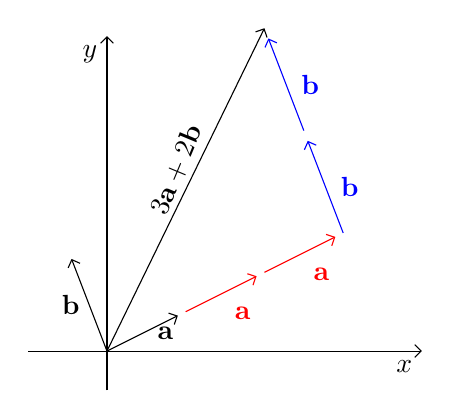
\begin{tikzpicture}[% styles used in image code
         > = Straight Barb, % defined in "arrows.meta
dot/.style = {circle, fill,
              minimum size=2mm, inner sep=0pt, outer sep=0pt,
              node contents={}},
box/.style = {draw, thin, minimum  width=2mm, minimum height=4mm,
              inner sep=0pt, outer sep=0pt,
              node contents={}, sloped},
my angle/.style args = {#1/#2}{draw,->,
                               angle radius=#1,
                               angle eccentricity=#2,
                               } % angle label position!
                        ]
	% coordinate axis
	\draw[->] (-1, 0) -- (4,0) node[below left] {$x$};
	\draw[->] ( 0,-0.5) -- (0,4) node[below left] {$y$};

	\coordinate (O) at (0,0);
	\coordinate (a) at (1,0.5);
	\coordinate (b) at (-0.5,1.3);
	
	\draw [->] (O) --($0.9*(a)$) node[pos=0.5,right=2pt] {$\mathbf{a}$};
	\draw [->,red] (a) --($1.9*(a)$) node[pos=0.5,below right=2pt] {$\mathbf{a}$};
	\draw [->,red] ($2*(a)$) --($2.9*(a)$) node[pos=0.5,below right=2pt] {$\mathbf{a}$};
	\draw [->] (O) --($0.9*(b)$) node[pos=0.5,left] {$\mathbf{b}$};
	\draw [->,blue] ($3*(a)$) --($3*(a) + 0.9*(b)$) node[pos=0.5,right=2pt] {$\mathbf{b}$};
	\draw [->,blue] ($3*(a) + (b)$) --($3*(a) + 1.9*(b)$) node[pos=0.5,right=2pt] {$\mathbf{b}$};
	\draw [->] (O) --($3*(a) + 2*(b)$) node[pos=0.7,above left, rotate=67.38] {$3\mathbf{a}+2\mathbf{b}$};
	%\draw [->] (a) --($(a)+1.3*(r)$) node[pos=0.9,above,rotate=26.5] {$\mathbf{a}}$};
\end{tikzpicture}
\end{figure}






\section{Vector subspaces and spans}

\definition{Vector subspace}{
Suppose that $V$ is a vector space and $W$ is a subset of $V$. We call $W$ a \textit{vector subspace} if it satisfies the vector space axioms for the same definition of vector addition and scalar multiplication defined for $V$.
}

\noindent In practice it can be tedious to show all 10 axioms hold for the subset. However, many of the properties are automatically inherited from the known vector space. For example any subset of vectors will obviously satisfy commutativity and associativity. In the end it suffices to prove just 3 properties for the candidate subspace.

\theorem{Demonstration of a vector subspace}{
Let $W$ be a subset of a vector space $V$. $W$ is a vector subspace if and only if
\begin{enumerate}
	\item $W$ is a non-empty set,
	\item $W$ is closed under vector addition: $\mathbf{u},\mathbf{v}\in W \, \implies \, \mathbf{u}+\mathbf{v}\in W$,
	\item $W$ is closed under scalar multiplication: $\mathbf{u}\in W \, \text{and} \, k\in\mathbb{R} \, \implies \, k\mathbf{u}\in W$.
\end{enumerate}
In fact, we can merge the two closure properties into one: closure under linear combinations
\begin{gather*}
\forall \mathbf{u},\mathbf{v}\in W \quad \text{and} \quad \forall \alpha, \beta\in\mathbb{R} \\
\alpha \mathbf{u} + \beta \mathbf{v} \in W.
\end{gather*}
}

\example{Vector subspace of triples satisfying an equation}{

\noindent Consider the equation $2x -y + z = 0$. We want to study the set of all triples, $(x,y,z)$, that satisfy the equation (we might call such a triple a ``solution'' to the equation). The set of these triples are a subset, call it $W$, of the Euclidean vector space $\mathbb{R}^3$. Let's show that $W$ is a vector subspace of $\mathbb{R}^3$. \\ 

\noindent Firstly, the vector $(0,0,0)\in W$ because its components satisfy the equation: $2(0)-(0)+(0)$ indeed equals zero. Hence $W$ has at least one vector, that is, it is a non-empty set (it's also easy to see that, for example, $(1,1,-1)$ or $(1,2,0)$ are also members of $W$). Let $\mathbf{u}=(u_x, u_y, u_z)$ and $\mathbf{v}=(v_x, v_y, v_z)$ be two arbitrary triples in $W$. That means their components satisfy the equation, i.e. $2u_x -u_y + u_z = 0$ and $2v_x -v_y + v_z = 0$. For any real $\alpha$ and $\beta$ we therefore have
\begin{align*}
\alpha \mathbf{u} + \beta \mathbf{v} = (\alpha u_x + \beta v_x, \alpha u_y + \beta v_y, \alpha u_z + \beta v_z) = (w_x, w_y, w_z).
\end{align*}
We need to check whether the components of this resultant triple satisfies the defining equation of $W$.
\begin{align*}
2w_x -w_y + w_z &= 2(\alpha u_x + \beta v_x) - (\alpha u_y + \beta v_y) + \alpha u_z + \beta v_z \\
&= \alpha (\underbrace{2u_x -u_y + u_z}_{=0}) + \beta \underbrace{2v_x -v_y + v_z}_{=0}.
\end{align*}
Since the triple $\alpha \mathbf{u} + \beta \mathbf{v}$ has components satisfying the equation, we conclude that $\alpha \mathbf{u} + \beta \mathbf{v} \in W$. So $W$ is a non-empty subset of a vector space and $W$ is closed under linear combinations. Thus $W$ is a vector subspace.
}


\example{Vector subspace of functions satisfying a equation}{

\noindent Let $W$ be the set of solutions of the following differential equation
\begin{align*}
\frac{d^2 y}{dx^2} + 3 \frac{dy}{dx} - 2y = 0.
\end{align*}
Is $W$ a vector subspace of the vector space of all real valued functions with real domain, $V$? \\

\noindent Consider the zero function $0(x) = 0$ for all $x\in\mathbb{R}$. This function's first and second derivatives combine to give
\begin{align*}
\frac{d^2}{dx^2}(0(x)) + 3 \frac{d}{dx}(0(x)) - 2(0(x)) = 0
\end{align*}
and so $0(x) \in W$, which is therefore a non-empty subset of $V$. If we have two functions, $y_1(x)$ and $y_2(x)$, in $V$ then they satisfy
\begin{align*}
\frac{d^2 y_1}{dx^2} + 3 \frac{dy_1}{dx} - 2y_1 = 0 \\
\frac{d^2 y_2}{dx^2} + 3 \frac{dy_2}{dx} - 2y_2 = 0.
\end{align*}
For any constants $\alpha$ and $\beta \in \mathbb{R}$ the linear combination of these solutions, $y=\alpha y_1+\beta y_2$, gives
\begin{align*}
\frac{d^2 y}{dx^2} + 3 \frac{dy}{dx} - 2y &= \frac{d^2}{dx^2}(\alpha y_1+\beta y_2) + 3 \frac{d}{dx}(\alpha y_1+\beta y_2) - 2(\alpha y_1+\beta y_2) \\
 &= \alpha\left(\frac{d^2 y_1}{dx^2} + 3 \frac{dy_1}{dx} - 2y_1\right) + \beta\left(\frac{d^2 y_2}{dx^2} + 3 \frac{dy_2}{dx} - 2y_2\right) \\
 &= 0
\end{align*}
and therefore $\alpha y_1+\beta y_2 \in W$. So we have shown that $W$ is a non-empty subset of $V$ which is closed under linear combinations. Hence $W$ is a vector subspace of $V$.
}

In the previous example we \textit{verified} that a space satisfied the vector space axioms. Now let's generate a vector space out of some given vectors. We can use the idea of linear combinations to generate a whole set of vectors.

\definition{Span}{
Let $\mathcal{B} = \{\mathbf{v}_1, \dots, \mathbf{v}_n\}$ be a set of vectors from a vector space $V$. The span of these vectors is the set of all linear combinations of those vectors:
\begin{align*}
\text{SPAN}(\mathcal{B})  = \text{SPAN} (\mathbf{v}_1, \dots, \mathbf{v}_n) = \left\{ \alpha_1 \mathbf{v}_1 + \cdots + \alpha_n \mathbf{v}_n \, | \, \alpha_1, \dots, \alpha_n \in \mathbb{R}^n \right\}.
\end{align*}
This set forms a vector subspace of $V$. It is obviously non-empty because it at least contains the vectors of $\mathcal{B}$. It is also automatically closed under vector addition and scalar multiplication because those are exactly the operations we used to create all the vectors in the span! Therefore $\text{SPAN}(\mathcal{B})$ is a vector subspace of $V$. \\

\noindent Note: we say that a set of vectors, $\mathcal{B}$, spans a vector space $U$ if $\text{SPAN}(\mathcal{B})=U$.
}




\example{Span of 1 vector}{
Suppose we have a vector space $V$. For any single arbitrary vector of $\mathcal{V}$ we can form the span subspace:
\begin{align*}
\textbf{v} \in V \quad\implies\quad \text{SPAN}(\textbf{v}) = \{k \textbf{v} \, | \, k\in\mathbb{R} \}
\end{align*}
If $V$ is $\mathbb{R}^2$, then this span is the line along the same direction of the arrow $\textbf{v}$:
\begin{figure}[H]
\centering
\begin{tikzpicture}[> = Triangle,scale=2]
	% coordinate axes
	\draw[->] (-1, 0) -- (3,0) node[right] {$x$};
	\draw[->] (0, -1) -- (0,2) node[left] {$y$};

	\coordinate (O) at (0,0); 
		
	% straight line y=x/2
	\draw[-,nicegreen,line width = 0.6mm] (-1,-0.5)--(3,1.5) node[left=10pt,darkgreen] {$\text{SPAN}(\textbf{v})$};
	
	% vectors u=(1,0.5) and v=(2,1)
	\draw[->,airforceblue,line width = 0.5mm] (O)--(1.2,0.6) node[below right,black] {$\textbf{v}=(x,y)$};
	%%%%%%%%%%%%%%%%%%%%%%%%%%%%%
\end{tikzpicture}
\end{figure}
\noindent If $V$ is, for example, the vector space of functions continuous on a given intervel, this span is a set of constant multiples of some function in $V$:
\begin{figure}[H]
\centering
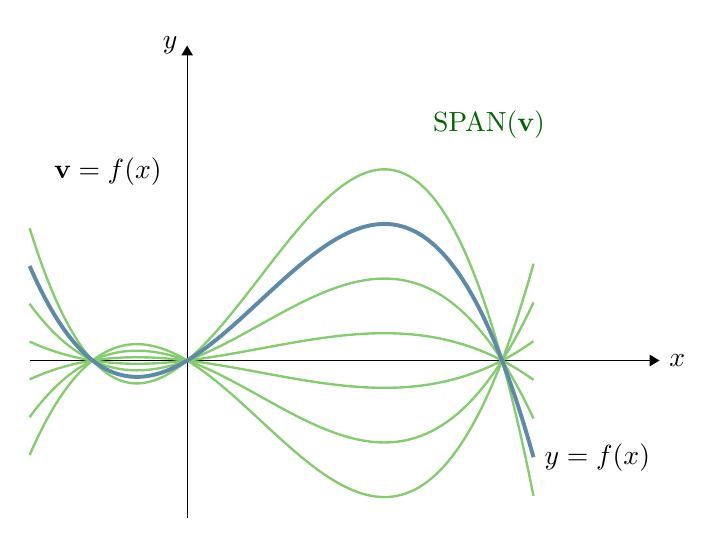
\begin{tikzpicture}[> = Triangle,scale=2]
	% coordinate axes
	\draw[->] (-1, 0) -- (3,0) node[right] {$x$};
	\draw[->] (0, -1) -- (0,2) node[left] {$y$};


	\coordinate (O) at (0,0); 
	\draw[smooth,variable=\x,samples=100,domain=-1:2.2,nicegreen,line width=0.3mm] plot({\x},{-0.7*(\x+0.6)*\x*(\x-2)});
	\draw[smooth,variable=\x,samples=100,domain=-1:2.2,nicegreen,line width=0.3mm] plot({\x},{-0.3*(\x+0.6)*\x*(\x-2)});
	\draw[smooth,variable=\x,samples=100,domain=-1:2.2,nicegreen,line width=0.3mm] plot({\x},{-0.1*(\x+0.6)*\x*(\x-2)});
	\draw[smooth,variable=\x,samples=100,domain=-1:2.2,nicegreen,line width=0.3mm] plot({\x},{+0.1*(\x+0.6)*\x*(\x-2)});
	\draw[smooth,variable=\x,samples=100,domain=-1:2.2,nicegreen,line width=0.3mm] plot({\x},{+0.3*(\x+0.6)*\x*(\x-2)});
	\draw[smooth,variable=\x,samples=100,domain=-1:2.2,nicegreen,line width=0.3mm] plot({\x},{+0.5*(\x+0.6)*\x*(\x-2)});
	\draw[smooth,variable=\x,samples=100,domain=-1:2.2,airforceblue,line width=0.5mm] plot({\x},{-0.5*(\x+0.6)*\x*(\x-2)}) node[right,black] {$y=f(x)$};
	
	\node[black,left] at (-0.1,1.2) {$\textbf{v}=f(x)$};
	\node[darkgreen,right] at (1.5,1.5) {$\text{SPAN}(\textbf{v})$};
	%%%%%%%%%%%%%%%%%%%%%%%%%%%%%
\end{tikzpicture}
\end{figure}
\noindent Of course these are not all of the functions in the span, as that would be a filled block of green. 
}

\noindent In 3d Euclidean space, the span of any two vectors pointing in different directions will form a plane. In the picture below we see some linear combinations of $\mathbf{a}$ and $\mathbf{b}$. Hopefully you can convince yourself that no such linear combination could leave the blue plane. We will prove this later.

\begin{figure}[H]
\centering
\tdplotsetmaincoords{105}{-30}
\begin{tikzpicture}[tdplot_main_coords,font=\sffamily]
  \tdplotsetrotatedcoords{00}{30}{0}
  \begin{scope}[tdplot_rotated_coords]
  \begin{scope}[canvas is xy plane at z=0]
    \fill[blue,fill opacity=0.1] (-3.5,-5) rectangle (2,4); 
    \path (-150:2) coordinate (H) (-1.5,0) coordinate(X);
   
    \coordinate (O) at (0,0);
    \coordinate (a) at (-1,1.8);
    \coordinate (b) at (-2,-1);
    \draw [->,red] (O) --($(a)$) node[pos=0.6,below=1pt] {$\mathbf{a}$};
    \draw [->,red] (O) --($(b)$) node[pos=0.6,right=1pt] {$\mathbf{b}$};
    
    \draw [->] (O) --($(a)+(b)$) node[pos=1,above=1pt] {$\mathbf{a}+\mathbf{b}$};
    \draw [->,blue] ($(a)+0.05*(b)$) --($(a)+0.9*(b)$) node[pos=0.5,left=1pt] {$\mathbf{b}$};
    
    \draw [->] (O) --($(b)-2*(a)$) node[pos=1,right=1pt] {$\mathbf{b}-2\mathbf{a}$};
    \draw [->,blue] ($(a)-0.1*1.2*(b)$) --($(a)-0.9*1.2*(b)$) node[pos=0.8,left=1pt] {$-1.2\mathbf{b}$};
    
    \draw [->] (O) --($(a)-1.2*(b)$) node[pos=1,right=1pt] {$\mathbf{a}-1.2\mathbf{b}$};
    \draw [->,blue] ($(b)-0.1*2*(a)$) --($(b)-0.9*2*(a)$) node[pos=0.7,above=1pt] {$-2\mathbf{a}$};
    
   
   \pgflowlevelsynccm
  \end{scope} 
 \end{scope}
 \pgfmathsetmacro{\Radius}{1.5}
 
 
 \draw[-stealth] (O)-- (2.5*\Radius,0,0) node[pos=1.15] {$y$};
 \draw[-stealth] (O) -- (0,3.5*\Radius,0) node[pos=1.15] {$x$};
 \draw[-stealth] (O) -- (0,0,2.5*\Radius) node[pos=1.05] {$z$};
\end{tikzpicture}\caption*{Some selected linear combinations, the black arrows, of $\mathbf{a}$ and $\mathbf{b}$.}
\end{figure}



\example{Checking whether a vector belongs to a span}{

\noindent Let $\mathbf{u}=(1,1,2)$ and $\mathbf{v}=(0,3,1)$ be two Euclidean vectors. Let $\text{SPAN}(\mathbf{u},\mathbf{v})=V$. Does the vector $\mathbf{w}=(1,-5,0)$ belong to $V$? \\

\noindent We need to check whether $\mathbf{w}$ really is a linear combination of $\mathbf{u}$ and $\mathbf{v}$ or not. If it is, then we can write:
\begin{align*}
\mathbf{w} = \alpha \mathbf{u} + \beta \mathbf{v}
\end{align*}
for some $\alpha$ and $\beta$ that we can find or else we will find a contradiction. We have assumed
\begin{align*}
(1,-5,0) &= \alpha(1,1,2) + \beta (0,3,1) \\
&= (\alpha,\alpha + 3\beta,2\alpha+\beta)
\end{align*}
giving the 3 equations
\begin{align*}
\alpha=1, \quad \alpha + 3\beta=-5, \quad 2\alpha+\beta = 0
\end{align*}
Putting the value of $\alpha$ into either the second or third gives the same result: $\beta = -2$. Importantly $(\alpha,\beta)=(1,-2)$ does not contradict the second equation. Hence $\mathbf{w}$ is a linear combination of $\mathbf{u}$ and $\mathbf{v}$
\begin{align*}
\mathbf{w}=\mathbf{u}-2\mathbf{v}
\end{align*}
and therefore $\mathbf{w}\in V$. Note that if we had shown that $\alpha$ and $\beta$ were impossible to exist, then this would mean $\textbf{w} \notin V$.
}

\definition{Cartesian form of Euclidean vector subspaces}{
Euclidean vector sub spaces can always be written as a set with some defining equations, called the Cartesian form:
\begin{align*}
\left\{ (x_1,\dots,x_n) \in \mathbb{R}^n \, | \, \text{equations relating the } x_k \right\}.
\end{align*}
For example, the general form of planar vector subspaces of $\mathbb{R}^3$ is
\begin{align*}
V_P = \left\{ (x,y,z)\in \mathbb{R}^3 \, | \, ax + by + cz = 0\right\}
\end{align*}
where $a$, $b$ and $c$ are some given constants. This set is read aloud as ``all the triples $(x,y,z)$ such that $ax + by + cz = 0$''.
}


\example{Second method to check whether a vector belongs to a span}{

\noindent Let's take up the previous example and answer it with a second method. Let $\mathbf{u}=(1,1,2)$ and $\mathbf{v}=(0,3,1)$ be two Euclidean vectors. Let $\text{SPAN}(\mathbf{u},\mathbf{v})=V$. Does the vector $\mathbf{w}=(1,-5,0)$ belong to $V$? \\

\noindent First we'll find an equation that defines this span. By definition
\begin{align*}
V = \{\alpha \mathbf{u} + \beta \mathbf{v} \, | \, \alpha, \beta  \in \mathbb{R}\}.
\end{align*}
So a generic vector $(x,y,z)$ in $V$ must satisfy
\begin{align*}
(x,y,z) &= \alpha (1,1,2) + \beta (0,3,1).
\end{align*}
Let's look for a single equation relating the $x$, $y$ and $z$:
\begin{align*}
(x,y,z) =  (\alpha,\alpha + 3\beta,2\alpha + \beta) 
\implies
\begin{cases}
x=\alpha \\
y=\alpha + 3\beta \\
z=2\alpha + \beta
\end{cases}
\implies
\begin{cases}
x=\alpha \\
y=x + 3\beta \\
z=2x + \beta
\end{cases}
\implies
\begin{cases}
x=\alpha \\
y=x + 3\beta \\
y-3z=-5x
\end{cases}
\end{align*}
This last line gives us the equation that all vectors of $V$ must satisfy, and so we have its Cartesian form:
\begin{align*}
V = \{(x,y,z)\in\mathbb{R}^3 \, | \, 5x + y - 3z = 0 \}.
\end{align*}
With this equation we can easily check whether $\mathbf{w}=(1,-5,0)$ belongs to $V$ or not:
\begin{align*}
5w_x + w_y - 3w_z = 5(1)+(-5)-3(0) = 0.
\end{align*}
The equation is satisfied and so $\mathbf{w}\in V$.
}


\example{Span of two 3d vectors in Cartesian form}{

\noindent Given the vectors
\begin{align*}
\textbf{v}_1 = (3,-1,1) \quad\text{and}\quad \textbf{v}_2 = (1,2,0)
\end{align*}
what is the Cartesian form of the span of these vectors, SPAN($\textbf{v}_1,\textbf{v}_2$)? \\

\noindent Consider an arbitrary triple in this space: $(x,y,z) \in \text{SPAN}(\textbf{v}_1,\textbf{v}_2)$. To be in this span means to be a linear combination: 
\begin{align*}
(x,y,z) = \alpha\textbf{v}_1 + \beta\textbf{v}_2
\end{align*}
for constants $\alpha$, $\beta$. This can be expanded 
\begin{align*}
(x,y,z) = \alpha(3,-1,1) + \beta(1,2,0) = (3\alpha + \beta,-\alpha + 2\beta,\alpha)
\end{align*}
to give the system of equations
\begin{align*}
\begin{cases}
x = 3\alpha + \beta \\
y = -\alpha + 2\beta \\
z = \alpha 
\end{cases}
\quad\implies\quad
2x - y - 7z = 0
\end{align*}
Which finally means that we have the Cartesian form
\begin{align*}
\text{SPAN}(\,(3,-1,1),(1,2,0)\,) = \left\{(x,y,z)\in\mathbb{R}^3 \, | \, 2x - y - 7z = 0\right\}
\end{align*}
As $2x - y - 7z = 0$ is a plane equation, this span creates a planar vector space.
}

\theorem{Span of two 3d vectors gives a plane}{
For any two 3d Euclidean vectors, $\textbf{u},\textbf{v}\in \mathbb{R}^3$, if they do not point in the same direction ($\textbf{u}\neq k\textbf{v}$ for some constant $k$) then their span gives a planar vector subspace of $\mathbb{R}^3$.
}

\begin{proof}
Let $\mathbf{u}=(u_x,u_y,u_z)$, $\mathbf{v}=(v_x,v_y,v_z)$ and $(x,y,z)\in \text{SPAN}(\mathbf{u},\mathbf{v})$. Then we must have some constants $\alpha,\beta \in \mathbb{R}$ such that
\begin{align*}
(x,y,z) &= \alpha \mathbf{u} + \beta \mathbf{v} \\
&= (\alpha u_x + \beta v_x, \, \alpha u_y + \beta v_y, \, \alpha u_z + \beta v_z)
\end{align*}
So we have the system of equations
\begin{align*}
& \begin{cases}
x = \alpha u_x + \beta v_x \\
y = \alpha u_y + \beta v_y \\
z = \alpha u_z + \beta v_z
\end{cases}
\implies
\begin{cases}
u_y x = \alpha u_x u_y  + \beta v_x u_y  \\
u_x y = \alpha u_x u_y + \beta v_y u_x \\
u_x z = \alpha u_x u_z + \beta v_z u_x \\
u_z x = \alpha u_x u_z + \beta v_x u_z 
\end{cases}
\implies
\begin{cases}
u_y x - u_x y = \beta (v_x u_y - v_y u_x) \\
u_z x - u_x z = \beta (v_x u_z -  v_z u_x)
\end{cases} \\
& \implies
\begin{cases}
(u_y x - u_x y)(v_x u_z -  v_z u_x) = \beta (v_x u_y - v_y u_x)(v_x u_z -  v_z u_x) \\
(u_z x - u_x z)(v_x u_y - v_y u_x) = \beta (v_x u_z -  v_z u_x)(v_x u_y - v_y u_x)
\end{cases} \\
& \implies
(u_y x - u_x y)(v_x u_z -  v_z u_x) - (u_z x - u_x z)(v_x u_y - v_y u_x) = 0
\end{align*}
A final rearrangement gives us our plane equation
\begin{align*}
(v_y u_x u_z-  v_z u_x u_y)x + (v_z u_x^2 - v_x u_z u_x) y + (v_x u_y u_x - v_y u_x^2)z = 0
\end{align*}
\textit{Note}: if the two vectors pointed in the same direction, we could find a constant $k$ such that $\mathbf{v}=k\mathbf{u}$ which implies that $v_x=ku_x$, $v_y=ku_y$ and $v_z=ku_z$. Putting this into the plane equation gives
\begin{align*}
\underbrace{(ku_y u_x u_z-  ku_z u_x u_y)}_0x + \underbrace{(ku_z u_x^2 - ku_x u_z u_x)}_0 y + \underbrace{(ku_x u_y u_x - ku_y u_x^2)}_0z = 0
\end{align*}
Since the left side cancels to zero, we don't have a plane equation relating the $x$, $y$ and $z$ variables.
\end{proof}


\example{From Cartesian form to a span}{

\noindent Given the Cartesian form of a vector space
\begin{align*}
A = \left\{(x,y,z)\in\mathbb{R}^3 \, | \, x + 2y - 3z = 0\right\}
\end{align*}
write $A$ in the form of a span of vectors. \\

\noindent We can rearrange the equation to $x=3z-2y$. So, every vector in $A$ can be written
\begin{align*}
(x,y,z) &= (3z-2y, y, z) \\
&= (-2y, y, 0) + (3z, 0, z) \\
&= y(-2, 1, 0) + z(3, 0, 1)
\end{align*}
With no further equations relating $y$ and $z$ to each other, they are free variables. This means $y$ and $z$ can take on any value. This means every triple $(x,y,z)\in A$ can be written as some linear combination of the vectors $\textbf{v}=(-2,1,0)$ and $\textbf{u}=(3,0,1)$. That is
\begin{align*}
A = \text{SPAN}( \, (-2,1,0), \, (3,0,1) \, )
\end{align*}
}


\section{Intersection, union and sum of subspaces}
The span vector space let us generate vector spaces out of given vectors. Now we look at generating vector spaces out of other vector spaces. As vector spaces are sets, it's natural to first consider the normal ways of combining sets: the intersection and union.

\theorem{Intersection of vector subspaces is a vector subspace}{
Suppose $V$ is a vector space. If $U$ and $W$ are two vector subspaces of $V$, then their intersection $U \cap W$ is also a vector subspace of $V$.}

\begin{proof} Let's show the two sufficient properties:
\begin{enumerate}
\item Non-empty - $U$ and $W$ must both contain the zero vector of $V$. Hence their intersection also contains the zero vector, and is thus a non-empty subset of $V$.

\item Closure under linear combinations - Let $\textbf{a}, \textbf{b} \in U \cap W$ and $\alpha, \beta \in \mathbb{R}$. Then $\textbf{a}, \textbf{b} \in U$, which is closed under linear combinations by being a vector space, and so $\alpha\textbf{a}+\beta\textbf{b} \in U$. But $\textbf{a}, \textbf{b} \in W$ also, which is closed under linear combinations, and so $\alpha\textbf{a}+\beta\textbf{b} \in W$. Hence
\begin{align*}
\alpha\textbf{a}+\beta\textbf{b} \in U\cap W
\end{align*}
and we have that the intersection is a vector subspace.
\end{enumerate}
\end{proof} 



For a visual example, consider the intersection of two planes in $\mathbb{R}^3$, $U$ and $V$, as pictured below.

\begin{figure}[H]
\begin{center}
    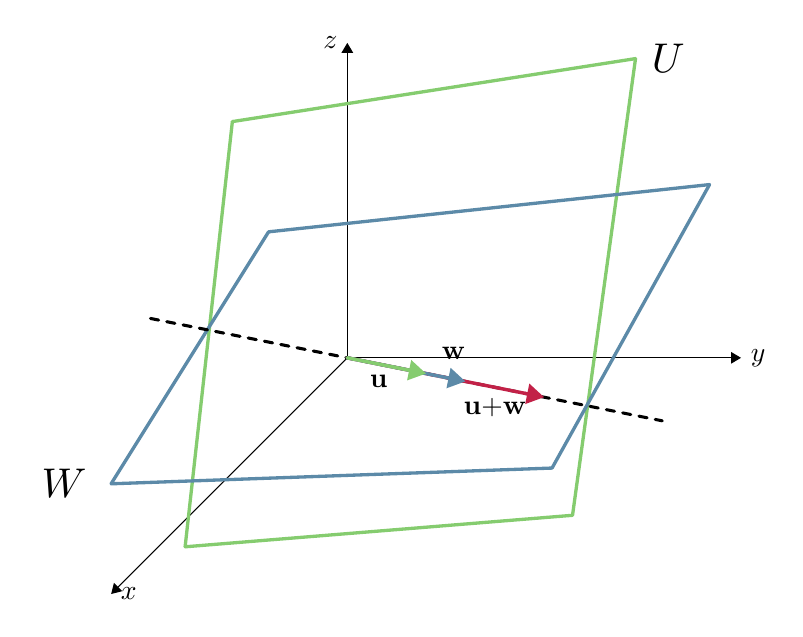
\begin{tikzpicture}[line cap=round, line join=round, >=Triangle,scale=2]

		% coordinate system
		\coordinate (O) at (0,0);
		\draw [->,black] (O)--(-1.5,-1.5) node[right] {$x$}; % x-axis
		\draw [->,black] (O)--(+2.5,+0.0) node[right] {$y$}; % y-axis
		\draw [->,black] (O)--(+0.0,+2.0) node[left] {$z$}; % z-axis
    
	    % plane 1 vertices positions
    	\coordinate (A1) at (-1.03,-1.2);
    	\coordinate (B1) at (-0.73,+1.5);
    	\coordinate (C1) at (+1.83,+1.9);
    	\coordinate (D1) at (+1.43,-1.0);
    	
	    % plane 2 vertices positions
    	\coordinate (A2) at (-1.5,-0.8);
    	\coordinate (B2) at (-0.5,+0.8);
    	\coordinate (C2) at (+2.3,+1.1);
    	\coordinate (D2) at (+1.3,-0.7);
    	
		\draw [-,nicegreen,line width=1.2pt] (A1)--(B1);
		\draw [-,nicegreen,line width=1.2pt] (B1)--(C1) node[right,black,pos=1,scale=1.5] {$U$};
		\draw [-,nicegreen,line width=1.2pt] (C1)--(D1);
		\draw [-,nicegreen,line width=1.2pt] (D1)--(A1);
    	
		\draw [-,airforceblue,line width=1.2pt] (A2)--(B2)node[left=3pt,black,pos=0,scale=1.5] {$W$};
		\draw [-,airforceblue,line width=1.2pt] (B2)--(C2);
		\draw [-,airforceblue,line width=1.2pt] (C2)--(D2);
		\draw [-,airforceblue,line width=1.2pt] (D2)--(A2);

		% vectors
		\coordinate (u) at (0.5,-0.1);
		\coordinate (w) at ($1.5*(u)$);
		\draw [dashed,black,line width=1.1pt] ($-2.5*(u)$)--($4*(u)$);
		\draw [->,brightmaroon,line width=1.25pt] (O)--($(u)+(w)$) node[below,black,pos=0.75] {\textbf{u}+\textbf{w}};
		\draw [->,airforceblue,line width=1.25pt] (O)--(w) node[above=3pt,black,pos=0.9] {\textbf{w}};
		\draw [->,nicegreen,line width=1.25pt] (O)--(u) node[below,black,pos=0.4] {\textbf{u}};
    \end{tikzpicture}
\end{center}
\end{figure}
The two planes must cross through $(0,0,0)$ to be subspaces (why?). The line of intersection will be a new subspace of $\mathbb{R}^3$. Of course any two vectors on this line will add up to a new vector still on the line.


\theorem{Union of vector subspaces}{
Suppose $V$ is a vector space. If we have 2 subspaces $U$ and $W$, then either
\begin{enumerate}
\item $U$ is a subspace of $W$
\item $W$ is a subspace of $U$
\item The union of $U$ and $W$ is NOT a subspace of $V$.
\end{enumerate}
}


\noindent To illustrate the third point, consider two straight lines in $\mathbb{R}^2$, $U$ and $V$.

\begin{figure}[H]
\begin{center}
    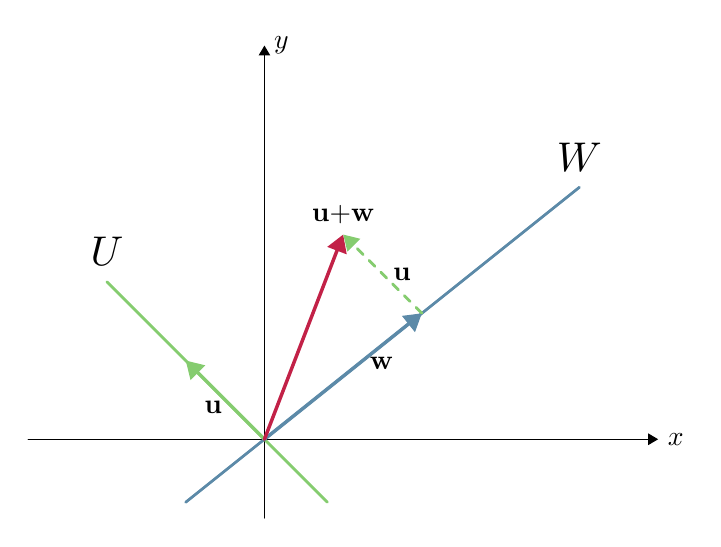
\begin{tikzpicture}[line cap=round, line join=round, >=Triangle,scale=2]
		% coordinate system
		\coordinate (O) at (0,0);
		\draw [->,black] (-1.5,0)--(+2.5,0) node[right] {$x$}; % x-axis
		\draw [->,black] (0,-0.5)--(0,+2.5) node[right] {$y$}; % y-axis
		
    	\coordinate (u) at (-0.5,+0.5);
    	\coordinate (w) at (1,0.8);
    	
		\draw [-,nicegreen,line width=1pt] ($-0.8*(u)$)--($2*(u)$) node[above,black,pos=1,scale=1.5] {$U$};
    	\draw [-,airforceblue,line width=1pt] ($-0.5*(w)$)--($2*(w)$) node[above,black,pos=1,scale=1.5] {$W$};
		
		\draw [->,nicegreen,line width=1.25pt] (O)--(u) node[left,black,pos=0.4] {\textbf{u}};
		\draw [->,airforceblue,line width=1.25pt] (O)--(w) node[right,black,pos=0.6] {\textbf{w}};
    	\draw [->,brightmaroon,line width=1.25pt] (O)--($(u)+(w)$) node[above,black] {\textbf{u}+\textbf{w}};
    	\draw [->,dashed,nicegreen,line width=1.0pt] (w)--($(u)+(w)$) node[right,black,pos=0.5] {$\textbf{u}$};

    \end{tikzpicture}
\end{center}
\end{figure}

\noindent The two lines must cross through $(0,0)$ to be subspaces. Remember that the union of two sets are all the members of both sets. For these two lines, the union will not be a new subspace of $\mathbb{R}^2$ because it is clearly not closed under vector addition. A simple example of this lack of closure is shown: any $\textbf{u}+\textbf{v}$ for $\textbf{u}\in U$ and $\textbf{v}\in V$ (and not the zero vectors) is clearly not going to remain in either $U$ or $V$.



\definition{Sum of subspaces (sum space)}{

Suppose we have a vector space $V$ with vector subspaces $F$ and $G$. We define the \textbf{sum of subspaces} (or sum space) as a new set denoted
\begin{align*}
F + G = \left\{ \textbf{f} + \textbf{g} \, | \, \textbf{f}\in F, \, \textbf{g}\in G\right\}
\end{align*}

\textit{Note}: The sum space is a \textit{subset} of the parent vector space: $F+G \subset V$.
}


\theorem{Sum space is a vector subspace}{
Let $F$ and $G$ be vector subspaces of $V$. The sum space $F+G$ is also a vector subspace of $V$.
}

\begin{proof} Let's show the two sufficient properties:
\begin{enumerate}
\item Non-empty. As $F$ is a vector space it must have at least the zero vector $\textbf{0}_V$. As $G$ is a vector space it cannot be empty, so it has at least some vector $\textbf{g}\in G$ (this could possibly be only the zero vector). The addition of these two vectors must be in the sum space: $\textbf{0}_V+\textbf{g}=\textbf{g}\in F+G$. So $F+G$ is not empty.

\item Closure. Let $\textbf{v}$ and $\textbf{w} \in F+G$ and $\alpha,\beta \in \mathbb{R}$. By definition the vectors can be written as the sum of vectors in $F$ and $G$: $\textbf{v}=\textbf{f}_1+\textbf{g}_1$ and $\textbf{w}=\textbf{f}_2+\textbf{g}_2$. The linear combination is thus
\begin{align*}
\alpha \textbf{v} + \beta \textbf{w} = \alpha\textbf{f}_1+\beta\textbf{f}_2+\alpha\textbf{g}_1+\beta\textbf{g}_2
\end{align*}
As $F$ and $G$ are vector spaces, they are closed under linear combinations. So $\alpha\textbf{f}_1+\beta\textbf{f}_2\in F$ and $\alpha\textbf{g}_1+\beta\textbf{g}_2 \in G$. Hence $\alpha \textbf{v} + \beta \textbf{w} = \textbf{f} + \textbf{g}$ for some $\textbf{f}\in F$ and $\textbf{g}\in G$, and thus $\alpha \textbf{v} + \beta \textbf{w} \in F+G$.
\end{enumerate}
\end{proof}


\noindent For a visual example of the sum of two subspaces. Consider two lines in $\mathbb{R}^2$ that pass through the origin. As we saw earlier that their union is not a vector subspace. But the sum of the two subspaces ($U$ and $W$ in the picture) includes all the possible vectors that can be reached by a sum of a vector belonging to each line:

\begin{figure}[H]
\begin{center}
    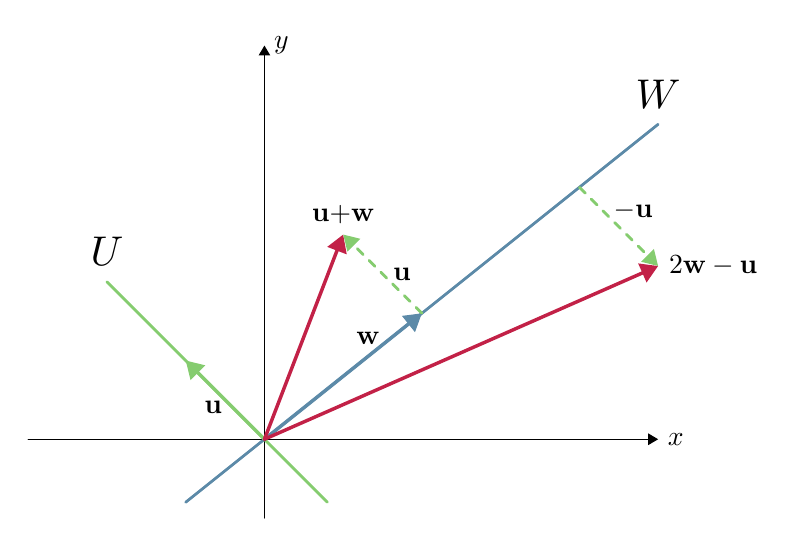
\begin{tikzpicture}[line cap=round, line join=round, >=Triangle,scale=2]
		% coordinate system
		\coordinate (O) at (0,0);
		\draw [->,black] (-1.5,0)--(+2.5,0) node[right] {$x$}; % x-axis
		\draw [->,black] (0,-0.5)--(0,+2.5) node[right] {$y$}; % y-axis
		
    	\coordinate (u) at (-0.5,+0.5);
    	\coordinate (w) at (1,0.8);
    	
		\draw [-,nicegreen,line width=1pt] ($-0.8*(u)$)--($2*(u)$) node[above,black,pos=1,scale=1.5] {$U$};
    	\draw [-,airforceblue,line width=1pt] ($-0.5*(w)$)--($2.5*(w)$) node[above,black,pos=1,scale=1.5] {$W$};
		
		\draw [->,nicegreen,line width=1.25pt] (O)--(u) node[left,black,pos=0.4] {$\textbf{u}$};
		\draw [->,airforceblue,line width=1.25pt] (O)--(w) node[left,black,pos=0.8] {$\textbf{w}$};
    	\draw [->,brightmaroon,line width=1.25pt] (O)--($(u)+(w)$) node[above,black] {\textbf{u}+\textbf{w}};
    	\draw [->,dashed,nicegreen,line width=1.0pt] (w)--($(u)+(w)$) node[right,black,pos=0.5] {$\textbf{u}$};
    	\draw [->,dashed,nicegreen,line width=1.0pt] ($2*(w)$)--($-1*(u)+2*(w)$) node[right,black,pos=0.3] {$-\textbf{u}$};
    	\draw [->,brightmaroon,line width=1.25pt] (O)--($-1*(u)+2*(w)$) node[right,black] {$2\textbf{w}-\textbf{u}$};

    \end{tikzpicture}
\end{center}
\end{figure}
\noindent Incidentally, in this example, the vector space $U + W$ is equal to all $\mathbb{R}^2$.

You should ask yourself ``how is the sum space different to the span''? The concept of sum space will later let us understand how to decompose vector spaces into constituent \textit{vector spaces}, whereas the span let's us consider the \textit{vectors} themselves as the generating objects.

\theorem{Smallest vector space containing a union of vector spaces}{
Let $F$ and $G$ be vector subspaces of a vector space $V$. Then $F+G$ is the smallest vector subspace of $V$ that contains the union $F \cup G$.
}

\definition{Direct sum}{
Let $F$ and $G$ be two vector subspaces of a vector space $V$ and let $E=F+G$ be the sum space. We say $E$ is a \textbf{direct sum} of $F$ and $G$ if each element of $E$ has a \textbf{unique} decomposition as a sum of vectors in $F$ and vectors in $G$. That is, for every $\textbf{v}\in E$, there exists unique vectors $\textbf{f}\in F$ and $\textbf{g}\in G$ such that $\textbf{v} = \textbf{f} + \textbf{g}$. We denote this direct sum with a new symbol
\begin{align*}
E = F \oplus G
\end{align*}
}

\noindent Lets build intuition by starting with an example of a sum space that is not a direct sum. 

\example{Sum of two planar vector spaces}{
Consider the following two vector subspaces of $\mathbb{R}^3$
\begin{align*}
A = \left\{ (x,y,z) \in\mathbb{R}^3 \, | \, x+y+z=0  \right\} \quad\text{and}\quad
B = \left\{ (x,y,z) \in\mathbb{R}^3 \, | \, x-y+z=0  \right\}.
\end{align*}
Is $A+B$ a direct sum of $A$ and $B$? \\

\noindent Let $\textbf{v}$ be an arbitrary vector in the sum space $A+B$. Then we have
\begin{align*}
\textbf{v}= (x,y,z) = \textbf{a} + \textbf{b}
\end{align*}
for some $\textbf{a}=(a_x,a_y,a_z)\in A$ and $\textbf{b}=(b_x,b_y,b_z)\in B$. So we can write the system of 5 equations with 6 unknowns 
\begin{align*}
x &= a_x + b_x &\quad a_x + a_y + a_z = 0\\
y &= a_y + b_y &\quad b_x - b_y + b_z = 0 \\
z &= a_z + b_z
\end{align*}
Now the goal is to invert these equations to find $a_x$, $a_y$, $a_z$, $b_x$, $b_y$ and $b_z$ as functions of $x$, $y$ and $z$. We don't have enough equations to do this uniquely, so we end up with a free variable. There are infinite ways to write this, but lets look at the solution if we let $b_z=t$ for any $t\in \mathbb{R}$:
\begin{align*}
a_x &= \dfrac{x-y-z+2t}{2}, &\quad a_y &= \dfrac{-x+y-z}{2}, &\quad a_z &= z-t  \\
b_x &= \dfrac{x+y+z-2t}{2}, &\quad b_y &= \dfrac{x+y+z}{2},  &\quad b_z &= t
\end{align*}
Let's consider the triple $(1,1,1)$. We have
\begin{align*}
(1,1,1) &= \overbrace{\left(-\dfrac{1}{2},\, -\dfrac{1}{2}, \, 1\right)}^{\in A} + \overbrace{\left( \dfrac{3}{2}, \, \dfrac{3}{2}, \,0 \right)}^{\in B}, \quad \text{for t=0} \\
(1,1,1) &= \underbrace{\left( \dfrac{1}{2},\, -\dfrac{1}{2},\, 0\right)}_{\in A} + \underbrace{\left (\dfrac{1}{2}, \, \dfrac{3}{2}, \, 1 \right)}_{\in A}, \quad  \text{for t=1}.
\end{align*}
This shows we have 2 different sum decompositions of $(1,1,1)$. So $A+B$ cannot be a direct sum of $A$ and $B$ as we don't have \textit{unique} decompositions for all its vectors.
}

\noindent Now showing that a particular sum of subspaces gives rise to \textit{unique} sum decompositions is not necessarily straight forward. The next theorem gives us an easy method.

\theorem{Direct sum demonstration}{
Let $F$ and $G$ be two vector subspaces of $V$. Then $E=F+G$ is a direct sum of $F$ and $G$ if and only if the intersection of $F$ and $G$ contains only the zero vector:
\begin{align*}
F \cap G = \{\textbf{0}_V \}.
\end{align*}
}

\example{Intersection of two planes}{
Consider again the previous two vector subspaces of $\mathbb{R}^3$
\begin{align*}
A = \left\{ (x,y,z) \in\mathbb{R}^3 \, | \, x+y+z=0  \right\} \quad\text{and}\quad
B = \left\{ (x,y,z) \in\mathbb{R}^3 \, | \, x-y+z=0  \right\}.
\end{align*}
The defining equations of these sets are both planar equations. Thinking geometrically, the intersection of two planes is a line. So it's trivial to know $A \cap B \neq \{ (0,0,0)\}$. Let's show in detail exactly what this intersection set is.
\begin{align*}
A \cap B = \left\{ (x,y,z) \in\mathbb{R}^3 \, | \, x+y+z=0, \, x-y+z=0 \right\}
\end{align*}
These two equations as a system will have to be reduced. Adding them gives $x+z=0 \implies z = -x$. Subtracting them gives $y=0$. So every triple can be written $(x,y,z)=(x,0,-x)=(1,0,-1)x$ for arbitrary $x$. Thus the intersection is
\begin{align*}
A \cap B = \left\{ (1,0,-1)t \in\mathbb{R}^3 \, , \, \forall t\in \mathbb{R} \right\}= \text{SPAN}( \, (1,0,-1) \, )
\end{align*}
This set represents a straight line in the direction of $(1,0,-1)$. We expected a straight line when we take the intersection of two planes. Since the intersection contains more than just the zero vector, this shows that $A+B$ is not a direct sum of $A$ and $B$.
}



\example{Direct sum of a planar and a linear vector space}{

\noindent Consider the following two vector subspaces of $\mathbb{R}^3$
\begin{align*}
F = \left\{ (x,y,z) \in\mathbb{R}^3 \, | \, x+2y-z=0  \right\} \quad\text{and}\quad
G = \text{SPAN}( \, (2,0,1) \, ).
\end{align*}
Show that $\mathbb{R}^3$ is a direct sum of $F$ and $G$. \\

\noindent First we have to convert $G$ from vector form into Cartesian form (left as an exercise): 
\begin{align*}
G = \left\{ (x,y,z) \in\mathbb{R}^3 \, | \, y=0, \, x=2z \right\}
\end{align*}
Which gives the first representation of the intersection set 
\begin{align*}
F \cap G = \left\{ (x,y,z) \in\mathbb{R}^3 \, | \, x+2y-z=0, \, y=0, \, x=2z \right\}
\end{align*} 
Now we reduce the system of equations
\begin{align*}
\begin{cases}
x+2y-z=0 \\ y=0 \\ x=2z 
\end{cases}
\implies
\begin{cases}
x-z=0  \\ y=0 \\ x=2z 
\end{cases}
\implies
\begin{cases}
x=z \\ y=0  \\ x=2z 
\end{cases}
\end{align*}
The two equations $x=z$ and $x=2z$ imply $x=0$ and $z=0$. So we have shown that all 3 variables are necessarily zero. Hence
\begin{align*}
F \cap G = \left\{ (0,0,0)  \right\} = \left\{ \textbf{0}_{\mathbb{R}^3} \right\}
\end{align*} 
Let's now show that $F+G=\mathbb{R}^3$. Let $(x,y,z)\in \mathbb{R}^3$. We have to show that it is possible to write
\begin{align*}
(x,y,z) = (\alpha,\beta,\gamma) + (a,b,c)
\end{align*}
where $(\alpha,\beta,\gamma)\in F$ and $(a,b,c)\in G$. Expanding we get the equations
\begin{align*}
x = \alpha + a, \quad y = \beta + b, \quad z = \gamma + c \\
\alpha+2\beta-\gamma=0, \quad  b=0, \quad a=2c
\end{align*}
We want to rearrange these equations to know what $\alpha$, $\beta$, $\gamma$, $a$, $b$ and $c$ must be for a given triple $x$, $y$ and $z$.
\begin{align*}
\begin{cases}
x = \alpha + 2c \\
y = \beta \\
z = \gamma + c
\end{cases}
\implies
\begin{cases}
x + 2y - z =  \alpha + 2c + 2\beta - \gamma - c = c\\
x - 2z = \alpha - 2\gamma = \alpha - 2(\alpha+2\beta) = -\alpha-4y
\end{cases}
\end{align*}
So we have
\begin{align*}
\alpha = -x-4y + 2z, \quad \beta=y, \quad \gamma=-x-2y + 2z \\
a = 2x+4y-2z, \quad b=0, \quad c=x+2y-z
\end{align*}
and hence we can write any triple as the addition of vectors from $F$ and $G$
\begin{align*}
(x,y,z) = \underbrace{(-x-4y + 2z, \, y, \, -x-2y + 2z )}_{\in F} + \underbrace{(2x+4y-2z, \, 0, \, x+2y-z)}_{\in G}
\end{align*}
This shows $\mathbb{R}^3 \subset F + G$. Since it is trivial that $F+G \subset \mathbb{R}^3$, we have shown that $F+G=\mathbb{R}^3$. Adding that with $F \cap G  = \left\{ \textbf{0}_{\mathbb{R}^3} \right\}$, we have shown that $\mathbb{R}^3$ is a direct sum of $F$ and $G$: $\mathbb{R}^3=F \oplus G$.

\textit{Note}: the definition of the direct sum was about the sum space having \textit{unique} representations of the parent space. If you go through the proof closely, you can understand that the expression we derived:
\begin{align*}
(x,y,z) = (-x-4y + 2z, \, y, \, -x-2y + 2z ) + (2x+4y-2z, \, 0, \, x+2y-z)
\end{align*}
is the only possibly expression for vectors in this sum space. So it means every triple has this \textit{unique} addition of a vector in $F$ with a vector in $G$. To show that we have a direct sum also included the proof of unique sum decompositions, so we wasted effort by looking at the intersection. In this sense, the investigation of the intersection of the member spaces of the sum is better suited for proving the negative proposition, that a particular sum is \textit{not} a direct sum.
}


\definition{Complementary vector subspaces}{
Let $F$ and $G$ be two vector subspaces of $V$. $F$ and $G$ are called \textbf{complementary} if $V$ is a direct sum of $F$ and $G$. That is, if and only if
\begin{itemize}
\item $V = F+G$, and
\item $F \cap G = \{\textbf{0}_V \}$
\end{itemize}

Two examples will reveal the subtlety of this definition:
\begin{itemize}
\item For $A=\{ (x,y,z)\in \mathbb{R}^3 \, | \, y=2x \}$ and $B=\{ (x,y,z)\in \mathbb{R}^3 \, | \, y=-x \}$ we do not have the direct sum $\mathbb{R}^3=A \oplus B$ despite the intersection being only the zero vector.

\item For $A=\{ (x,y)\in \mathbb{R}^2 \, | \, y=2x \}$ and $B=\{ (x,y)\in \mathbb{R}^2 \, | \, y=-x \}$ we do have the direct sum $\mathbb{R}^2=A \oplus B$.
\end{itemize}
}

\noindent Finally, we have now defined a new type of addition. Don't be fooled by the plus symbol, the sum space is a specific definition of addition of whole vector spaces. However, this operation has parallels to normal number addition. We list some of these properties below.

\properties{of vector space summation}{

\noindent Let $F$, $G$, and $H$ be vector subspaces of a vector space $V$. The sum space satisfies the following properties:
\begin{itemize}
\item Associativity: $F + (G + H) = (F + G) + H$
\item Commutativity: $F + G = G + F$
\item Null element: $F + \{\textbf{0}_V\} = F$
\end{itemize}
}

\noindent While these properties are familiar properties of addition, there are also differences. For example, for any vector subspace $F$, the sum space $F+F=F$ (can you prove this?). This means there is no normal sense of scalar multiplication of vector spaces.





%%%%%%%%%%%%%%%%%%%%%%%%%%%
%%%%%%%%%%%%%%%%%%%%%%%%%%%
%%%%%%%%%%%%%%%%%%%%%%%%%%%
\section{Linear independence, bases and coordinates}
%%%%%%%%%%%%%%%%%%%%%%%%%%%
%%%%%%%%%%%%%%%%%%%%%%%%%%%
%%%%%%%%%%%%%%%%%%%%%%%%%%%
\subsection*{Linear dependence and independence}

\noindent When we considered the span of two 3d vectors giving a plane I casually inserted an important qualification, that the two vectors \textit{are not in the same direction}. If we have two vectors $\mathbf{u}$ and $\mathbf{v}$ in the same direction then, for example, $\mathbf{v}=k\mathbf{u}$ for some real $k$. Then any linear combination of these two vectors gives a third vector
\begin{align*}
\mathbf{w} &= \alpha \mathbf{u} + \beta \mathbf{v} \\
&= \alpha \mathbf{u} + \beta k\mathbf{u} \\
&= \left(\alpha + \beta k\right) \mathbf{u}
\end{align*}
that is, $\mathbf{w}$ must also be in the same direction as $\mathbf{u}$. The span of these 2 vectors gives only vectors in this single direction. In this case we say that $\mathbf{u}$ and $\mathbf{v}$ are not independent vectors. One can be represented in terms of the other. Let's formalise this notion of vector dependence.

\definition{Linear dependence}{
A set of vectors $\{\mathbf{v}_1, \dots, \mathbf{v}_n\}$ from a vector space $V$ is said to be \textit{linearly dependent} if there exists a set of constants $\{ \alpha_1, \dots, \alpha_n \}$ \textit{not all zero} such that
\begin{align*}
\alpha_1 \mathbf{v}_1 + \cdots + \alpha_n \mathbf{v}_n = \mathbf{0}_V.
\end{align*}
\textit{Note}: the right hand side of the equation is the \textit{zero vector}, not the real number $0$.
}

\example{Linear dependence of two Euclidean vectors}{

\noindent Let $\mathbf{u}=(1,2)$ and $\mathbf{v}=(10.2,20.4)$. Show that $\mathbf{u}$ and $\mathbf{v}$ are linearly dependent. \\

\noindent To show this we must demonstrate that there are two constants, $a$ and $b$, such that $a\mathbf{u} + b\mathbf{v} = \mathbf{0}$. If this was true, we would have
\begin{align*}
& a(1,2) + b(10.2,20.4) = (0,0) \\
\implies & (a + 10.2b,2a + 20.4b) = (0,0)
\end{align*}
giving the system of equations
\begin{align*}
\begin{cases}
a + 10.2b = 0 \\
2a + 20.4b = 0
\end{cases}
\end{align*}
Both equations give the same relation between $a$ and $b$:
\begin{align*}
b = -\frac{a}{10.2}
\end{align*}
We are free to choose an $a$, for example if $a=10.2$ then $b=-1$ and we have
\begin{align*}
10.2 \mathbf{u} - 1 \mathbf{v} = \mathbf{0}
\end{align*}
showing that the two vectors are linearly dependent. This example show that the linear dependence of 2 vectors means that 1 vector is a scalar multiple of the other. In this example:
\begin{align*}
\mathbf{v} = 10.2 \mathbf{u}.
\end{align*}
}

\noindent How does this definition relate to what we understood earlier, that two vectors are dependent on each other if one can be expressed in terms of the other? Well, consider three vectors $\mathbf{u}$, $\mathbf{v}$ and $\mathbf{w}\in \mathbb{R}^3$. If there exists some constants $\alpha$, $\beta$ and $\gamma$, \textit{not all zero}, such that
\begin{align*}
\alpha \mathbf{u} + \beta \mathbf{v} + \gamma \mathbf{w} = \mathbf{0}_V
\end{align*}
then we can write the vector with the non-zero constant in terms of the other. For example suppose $\alpha \neq 0$, then
\begin{align*}
\mathbf{u}  =-\frac{\beta}{\alpha} \mathbf{v} - \frac{\gamma}{\alpha} \mathbf{w}.
\end{align*}
In this way $\mathbf{u}$ depends on the other two, or we could say $\mathbf{u} \in \text{SPAN}(\mathbf{v},\mathbf{w})$. This also means that the span of the three vectors $\text{SPAN}(\mathbf{u},\mathbf{v},\mathbf{w})=\text{SPAN}(\mathbf{v},\mathbf{w})$. The vector $\mathbf{u}$ doesn't give anything new. 

For Euclidean vectors, when we have two vectors that are linearly dependent we say that they are \textit{colinear}, as pictured below.
\begin{figure}[H]
\begin{center}
    \begin{tikzpicture}[line cap=round, line join=round, >=Triangle,scale=2]
		% coordinate system
		\coordinate (O) at (0,0);
		\draw [->,black] (-1.5,0)--(+2.5,0) node[right] {$x$}; % x-axis
		\draw [->,black] (0,-0.5)--(0,+2.5) node[right] {$y$}; % y-axis
		
    	\coordinate (u) at (0.5,+0.4);
    	\coordinate (v) at (1.5,1.2);
    	
    	\draw [-,nicegreen,line width=1pt] ($-0.2*(v)$)--($2*(v)$)node[left=10pt,black,pos=0.8, scale=1.2] {$\text{SPAN}(\textbf{u},\textbf{v})$};
		
		\draw [->,brightmaroon,line width=1.25pt] (O)--(v) node[left,black,pos=0.8] {$\textbf{v}$};
		\draw [->,airforceblue,line width=1.25pt] (O)--(u) node[left=5pt,black,pos=0.8] {$\textbf{u}$};
    \end{tikzpicture}
\end{center}
\end{figure}

When we have three 3d Euclidean vectors that are linearly dependent we say that they are \textit{coplanar}. Any two of the vectors give a plane as their span and then adding the 3rd dependent vector gives linear combinations that remain in that plane, as pictured below.

\begin{figure}[H]
\begin{center}
    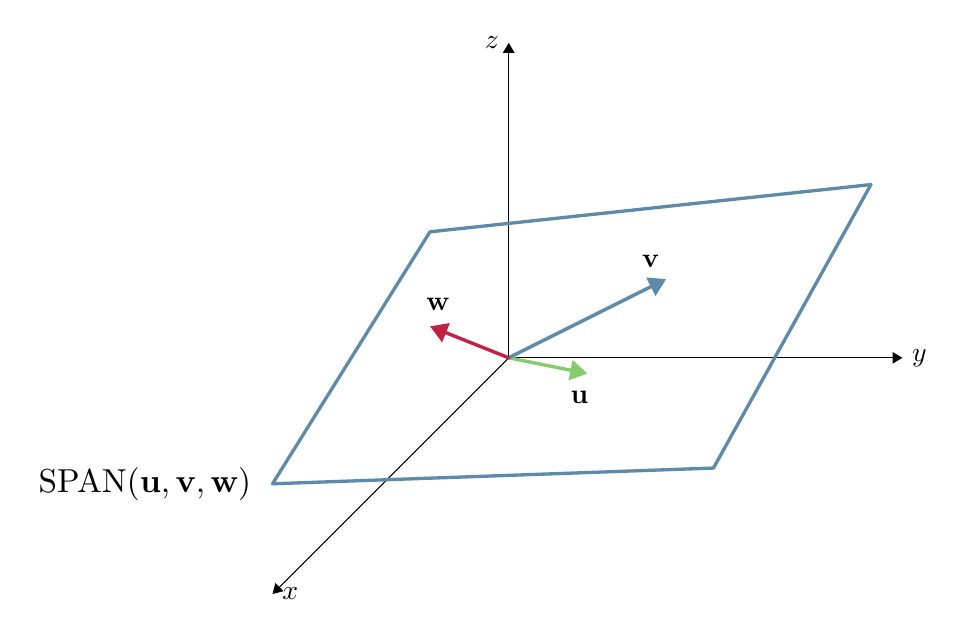
\begin{tikzpicture}[line cap=round, line join=round, >=Triangle,scale=2]

		% coordinate system
		\coordinate (O) at (0,0);
		\draw [->,black] (O)--(-1.5,-1.5) node[right] {$x$}; % x-axis
		\draw [->,black] (O)--(+2.5,+0.0) node[right] {$y$}; % y-axis
		\draw [->,black] (O)--(+0.0,+2.0) node[left] {$z$}; % z-axis
    
    	
	    % plane vertices positions
    	\coordinate (A) at (-1.5,-0.8);
    	\coordinate (B) at (-0.5,+0.8);
    	\coordinate (C) at (+2.3,+1.1);
    	\coordinate (D) at (+1.3,-0.7);
    	
    	
		\draw [-,airforceblue,line width=1.2pt] (A)--(B)node[left=3pt,black,pos=0,scale=1.2] {$\text{SPAN}(\textbf{u},\textbf{v},\textbf{w})$};
		\draw [-,airforceblue,line width=1.2pt] (B)--(C);
		\draw [-,airforceblue,line width=1.2pt] (C)--(D);
		\draw [-,airforceblue,line width=1.2pt] (D)--(A);

		% vectors
		\coordinate (u) at (0.5,-0.1);
		\coordinate (v) at (1,0.5);
		\coordinate (w) at (-0.5,0.2);
		\draw [->,nicegreen,line width=1.25pt] (O)--(u) node[below=3pt,black,pos=0.9] {$\textbf{u}$};
		\draw [->,airforceblue,line width=1.25pt] (O)--(v) node[above=3pt,black,pos=0.9] {$\textbf{v}$};
		\draw [->,brightmaroon,line width=1.25pt] (O)--(w) node[above=3pt,black,pos=0.9] {$\textbf{w}$};
    \end{tikzpicture}
\end{center}
\end{figure}

Now, what would it mean for a vector $\mathbf{u}$ to be independent of other vectors $\mathbf{v}$ and $\mathbf{w}$? The formal definition is simple:

\definition{Linear independence}{
A set of vectors $\{\mathbf{v}_1, \dots, \mathbf{v}_n\}$ from $V$ is said to be \textit{linearly independent} if they are not linearly dependent. That is, the equation
\begin{align*}
\alpha_1 \mathbf{v}_1 + \cdots + \alpha_n \mathbf{v}_n =  \mathbf{0}_V.
\end{align*}
implies that the constants $\alpha_1, \dots, \alpha_n$ \textit{are all zero}.
}

\noindent This definition is a little cheeky. Independent means not dependent. Let's understand it in the sense we were thinking earlier, where we think a vector $\mathbf{u}$ being independent of two other vectors $\mathbf{v}$ and $\mathbf{w}$ should mean that we cannot express $\mathbf{u}$ as a linear combination of $\mathbf{v}$ and $\mathbf{w}$. This follows from the definition. If we could write such a linear combination, then there are constants $\alpha$ and $\beta$ such that
\begin{align*}
\mathbf{u} &= \alpha \mathbf{u} + \beta \mathbf{v} \\
\implies & \mathbf{u}- \alpha \mathbf{u} - \beta \mathbf{v} = \mathbf{0}_V,
\end{align*}
but this equation is impossible as $\alpha_1 \mathbf{u} + \alpha_2 \mathbf{v} + \alpha_3 \mathbf{w} =  \mathbf{0}_V \implies \alpha_1=\alpha_2=\alpha_3=0$. \\


\example{Linear independence of three Euclidean vectors}{

\noindent Consider the following vectors in $\mathbb{R}^3$:
\begin{align*}
\mathbf{u} = (1,-1,1), \quad \mathbf{v} = (1,1,1), \quad \text{and} \quad \mathbf{w} = (2,2,4).
\end{align*}
Show that these three vectors are linearly independent. \\

\noindent We start with the equation
\begin{align*}
\alpha \mathbf{u} + \beta \mathbf{v} + \gamma \mathbf{w} = \mathbf{0}
\end{align*}
with the goal of finding possible solutions for $\alpha$, $\beta$ and $\gamma$. Writing the vector equation in full gives
\begin{align*}
& \alpha (1,-1,1) + \beta (1,1,1) + \gamma (2,2,4) = (0,0,0) \\
& (\alpha + \beta + 2\gamma, \, -\alpha + \beta + 2\gamma, \, \alpha + \beta + 4 \gamma) = (0,0,0)
\end{align*}
Component by component this vector equation is actually a system of equations
\begin{align*}
&\begin{cases}
\alpha + \beta + 2\gamma = 0 \\
-\alpha + \beta + 2\gamma = 0 \\
\alpha + \beta + 4\gamma = 0 
\end{cases}
\begin{matrix}
 \\
 L_2 \to L_2 + L_1 \\
 L_3 \to L_3 - L_1
\end{matrix}
\\
&\begin{cases}
\alpha + \beta + 2\gamma = 0 \implies \alpha = -\beta - 2\gamma \\
2\beta + 4\gamma = 0 \implies \beta = -2 \gamma \\
2\gamma = 0
\end{cases} 
\end{align*}
The last equation implies $\gamma=0$, which them implies $\beta=0$, which then implies $\alpha=0$. So the assumption that 
\begin{align*}
\alpha \mathbf{u} + \beta \mathbf{v} + \gamma \mathbf{w} = \mathbf{0}
\end{align*}
implies that $\alpha=\beta=\gamma=0$. That is exactly the definition of linear independence.
}


\example{Linear independence of three polynomial vectors}{

\noindent Consider the following vectors in the vector space of polynomials with degree up to two:
\begin{align*}
\mathbf{u} = 1 + x^2, \quad \mathbf{v} = x-2x^2, \quad \text{and} \quad \mathbf{w} = 3 - x.
\end{align*}
Show that these three vectors are linearly independent. \\

\noindent We start with the equation
\begin{align*}
\alpha \mathbf{u} + \beta \mathbf{v} + \gamma \mathbf{w} = \mathbf{0}
\end{align*}
with the goal of finding possible solutions for $\alpha$, $\beta$ and $\gamma$. Noting that the zero vector in the space of polynomials is the number 0, we write the vector equation in full
\begin{align*}
& \alpha ( 1 + x^2) + \beta (x-2x^2) + \gamma (3 - x) = 0 \\
& (\alpha + 3\gamma)1 + (\beta - \gamma)x + (\alpha - 2\beta)x^2 = (0)1 + (0)x + (0)x^2
\end{align*}
Equating the coefficients gives the system
\begin{align*}
\begin{cases}
\alpha + 3\gamma = 0 \implies \alpha = -\gamma/3 \\
\beta - \gamma = 0 \implies \beta = \gamma\\
\alpha - 2\beta = 0 \implies \alpha = 2\beta = 2\gamma
\end{cases}
\end{align*}
The only way that $\alpha = -\gamma/3$ and $\alpha = 2\gamma$ is for $\alpha=\gamma=0$. This then implies that $\beta=0$. We have therefore shown that
\begin{align*}
\alpha \mathbf{u} + \beta \mathbf{v} + \gamma \mathbf{w} = \mathbf{0}
\end{align*}
necessarily implies that $\alpha=\beta=\gamma=0$, and so these three vectors are linearly independent.
}

\noindent Take note of the simple logic or methodology of the previous three examples. We always start with the equation
\begin{align*}
\alpha_1 \mathbf{v}_1 + \alpha_2 \mathbf{v}_2 + \cdots + \alpha_n \mathbf{v}_n = \mathbf{0}_V
\end{align*}
and show either that by necessity all of the coefficients are zero (then the vectors are linearly independent), or that we can find at least one non-zero coefficients (then the vectors are linearly dependent). The exact method by which we determine these coefficients depends on which type of vectors we are considering.

\theorem{The span of a dependent set of vectors can be reduced}{
Let $\mathcal{B}=\{\mathbf{v}_1, \, \mathbf{v}_2, \, \dots, \mathbf{v}_n\}$ be a set of vectors of $V$. If $\mathcal{B}$ is a set of linearly dependent vectors, then we can always remove one of the vectors to form a new set, $\mathcal{B}'=\mathcal{B} \backslash \{\mathbf{v}_k\}$ for some $k$, without changing the span: $\text{SPAN}(\mathcal{B}')=\text{SPAN}(\mathcal{B})$.
}

\begin{proof}
Due to the linear dependence of the vectors of $\mathcal{B}$, there exists a set of constants $\alpha_1,\dots,\alpha_n \in \mathbb{R}$ not all zero such that
\begin{align*}
\alpha_1 \mathbf{v}_1 + \cdots + \alpha_n \mathbf{v}_n =  \mathbf{0}_V.
\end{align*}
Suppose $\alpha_k \neq 0$. Then we can write
\begin{align*}
\mathbf{v}_k = -\frac{\alpha_1}{\alpha_k} \mathbf{v}_1 - \cdots -\frac{\alpha_{k-1}}{\alpha_k} \mathbf{v}_{k-1} -\frac{\alpha_{k+1}}{\alpha_k}\mathbf{v}_{k+1} - \cdots -\frac{\alpha_n}{\alpha_k}  \mathbf{v}_n = -\sum_{i \neq k} \frac{\alpha_i}{\alpha_k} \mathbf{v}_i.
\end{align*}
which is to say $\mathbf{v}_k \in \text{SPAN}(\mathcal{B}')$ for $\mathcal{B}' = \left\{ \mathbf{v}_1, \, \cdots, \, \mathbf{v}_{k-1}, \,\mathbf{v}_{k+1}, \,  \mathbf{v}_n \right\}$. We want to prove that $\text{SPAN}(\mathcal{B}) = \text{SPAN}(\mathcal{B}')$. To show that two sets are equal we show that they are subsets of each other. That $ \text{SPAN}(\mathcal{B'}) \subset  \text{SPAN}(\mathcal{B})$ is trivial because $\mathcal{B}'$ is created out of $\mathcal{B}$ by only removing one vector. The other direction is more interesting. \\

\noindent Let $\mathbf{v} \in \text{SPAN}(\mathcal{B})$. Then we can find some set of constants $\beta_1$, \dots, $\beta_n$ not all zero such that
\begin{align*}
\mathbf{v} &= \beta_1 \mathbf{v}_1 + \cdots + \beta_k \mathbf{v}_k + \cdots + \beta_n \mathbf{v}_n \\
&= \beta_k \mathbf{v}_k + \sum_{i \neq k} \beta_i \mathbf{v}_i \\
&= \beta_k \left(-\sum_{i \neq k} \frac{\alpha_i}{\alpha_k} \mathbf{v}_i \right) + \sum_{i \neq k} \beta_i \mathbf{v}_i \\
&= \sum_{i \neq k} \left(\beta_i - \frac{\beta_k \alpha_i}{\alpha_k} \right)\mathbf{v}_i 
\end{align*}
This shows that $\mathbf{v}$ is a linear combination of vectors of $\mathcal{B}'$. So $\mathbf{v} \in \text{SPAN}(\mathcal{B}')$ and therefore $\text{SPAN}(\mathcal{B}) \subset  \text{SPAN}(\mathcal{B'})$.
\end{proof}


\noindent Now linear independence is a very important concept because it allows us to keep reducing the number of vectors in spans until we find a minimal set of vectors that are able to generate some vector space. Such a minimal set is called a basis, and is the focus of the next section.


\subsection*{Vector space basis}

\definition{Basis}{
A \textit{basis of a vector space} $V$ is a minimal set of vectors which spans the vector space. Formally, the set of vectors $\mathcal{B}=\{\mathbf{v}_1, \dots, \mathbf{v}_n\}$ in a vector space $V$ is a basis of $V$ if it is a set of linearly independent vectors and $\text{SPAN}(\mathbf{v}_1, \dots, \mathbf{v}_n) = V$. \textit{Note}: bases are not unique, but they always contain the same number of vectors.
}

\theorem{Bases of two dimensional Euclidean space}{
Any two linearly independent vectors in $\mathbb{R}^2$ forms a basis of $\mathbb{R}^2$.
}

\begin{proof}
Let $\mathbf{u}=(u_x,u_y)$ and $\mathbf{v}=(v_x,v_y)$ be two linearly independent vectors of $\mathbb{R}^2$. Since we've assumed the linear independence half of the definition of a basis, we only need to show that $\mathbb{R}^2 = \text{SPAN}(\mathbf{u},\mathbf{v})$. Let $(x,y)\in \mathbb{R}^2$. If $(x,y) \in \text{SPAN}(\mathbf{u},\mathbf{v})$ then we can find two constants $\alpha$ and $\beta \in \mathbb{R}$ such that
\begin{align*}
(x,y) &= \alpha \mathbf{u} + \beta \mathbf{v} \\
&= (\alpha u_x + \beta v_x, \,\alpha u_y + \beta v_y )
\end{align*}
which gives the system of equations
\begin{align*}
&
\begin{cases}
x = \alpha u_x + \beta v_x \\
y = \alpha u_y+ \beta v_y
\end{cases}
\\
\implies &
\begin{cases} 
u_y x - u_x y = (u_y  v_x  - u_x v_y) \beta \\
v_y x - v_x y = (v_y  u_x  - v_x u_y) \alpha
\end{cases}
\end{align*}
Now the linear independence of $\mathbf{u}$ and $\mathbf{v}$ means that the term in parentheses, $u_y  v_x  - u_x v_y$, is not zero. Why? Because if it was zero we would have
\begin{align*}
u_y  v_x = u_x v_y.
\end{align*}
We have some cases to consider here. If $v_y=0$, then either $u_y=0$ or $v_x=0$ (or both). 
\begin{itemize}
	\item If $v_x = 0$ then $\mathbf{v}=(0,0)=0\mathbf{u}$ and we have contradicted the assumption of linear independence. So we can't have $v_x = 0$.
	\item If $u_y=0$ then the two vectors become $\mathbf{u}=(u_x,0)$ and $\mathbf{v}=(v_x,0)$. Since $v_x$ cannot be zero we can write $\mathbf{u}=\dfrac{u_x}{v_x}\mathbf{v}$ and we have contradicted the assumption of linear independence. So we can't have $u_y=0$ . 
\end{itemize}
Since both outcomes are contradictions, we cannot have $v_y=0$. That is, we know $v_y\neq 0$. With that the equation $u_y  v_x = u_x v_y$ implies that neither $u_y$ nor $v_x$ can be zero and we can write
\begin{align*}
\frac{u_x}{u_y} = \frac{v_x}{v_y}.
\end{align*}
Then 
\begin{align*}
(u_x,u_y) &= u_y\left(\frac{u_x}{u_y},1\right) \\
          &= u_y\left(\frac{v_x}{v_y},1\right) \\
          &= \frac{u_y}{v_y}(v_x,v_y)
\end{align*}
and this contradicts the linear independence. So we simply can't have that $u_y  v_x  - u_x v_y=0$. All of that just so we can divide by this term, all the way back a long way to our system of equations to solve them for $\alpha$ and $\beta$:
\begin{align*}
 \alpha &= \frac{v_y x - v_x y}{v_y  u_x  - v_x u_y} \\
  \beta &= \frac{u_y x - u_x y}{u_y  v_x  - u_x v_y} 
\end{align*}
Now we can finally write any double in terms of $\mathbf{u}$ and $\mathbf{v}$:
\begin{align*}
(x,y) = \frac{v_y x - v_x y}{v_y  u_x  - v_x u_y}\mathbf{u} + \frac{u_y x - u_x y}{u_y  v_x  - u_x v_y} \mathbf{v}
\end{align*}
This shows that $\mathbb{R}^2 \subset \text{SPAN}(\mathbf{u},\mathbf{v})$. The other direction is automatic, and so we have proven that $\mathcal{B}=\{ \mathbf{u},\,\mathbf{v} \}$ is a basis of $\mathbb{R}^2$.
\end{proof}

\example{A basis of degree 1 polynomials}{

\noindent Consider a set of polynomial vectors $\mathcal{B}=\{ 1+x, \, 1-x \}$. Show that $\mathcal{B}$ is a basis of the vector space of polynomials with degree up to one, $\mathcal{P}_1$. \\

\noindent Let's start by showing the two vectors $\mathbf{b}_1 = 1+x$ and $\mathbf{b}_2=1-x$ are linearly independent. Assume
\begin{align*}
& \alpha \mathbf{b}_1 + \beta \mathbf{b}_2 = \mathbf{0} \\
\implies & \alpha (1+x) + \beta (1-x) = 0 \\
\implies & (\alpha + \beta)1 + (\alpha - \beta)x = (0)1 + (0)x
\end{align*}
which gives the system of equations
\begin{align*}
\begin{cases}
\alpha + \beta = 0 \\
\alpha - \beta = 0
\end{cases}
\end{align*}
Adding the equations gives $2\alpha = 0$ and subtracting gives $2\beta = 0$. So we have $\alpha=\beta=0$ and therefore $\mathbf{b}_1$ and $\mathbf{b}_2$ are linearly independent. Now let's prove that $\mathcal{P}_1 = \text{SPAN}(\mathbf{b}_1,\mathbf{b}_2)$. $\text{SPAN}(\mathbf{b}_1,\mathbf{b}_2) \subset \mathcal{P}_1$ is automatic. For the other direction, let $\mathbf{p}=(a)1+(b)x \in \mathcal{P}_1$ for some $a$, $b \in \mathbb{R}$. Then we want to find some $\alpha$, $\beta \in \mathbb{R}$ such that
\begin{align*}
\mathbf{p} &= \alpha\mathbf{b}_1+\beta\mathbf{b}_2 \\
\implies (a)1+(b)x &= \alpha (1+x) + \beta (1-x) \\
&= (\alpha + \beta)1 + (\alpha - \beta)x
\end{align*} 
and so
\begin{align*}
& \begin{cases}
a = \alpha + \beta \\
b = \alpha - \beta
\end{cases}
\\
\implies &
\begin{cases}
a+b = 2\alpha\\
a-b = 2\beta
\end{cases}
\\
\implies &
\begin{cases}
\alpha = \dfrac{a+b}{2} \\
\beta = \dfrac{a-b}{2} 
\end{cases}
\end{align*}
So we can write any polynomial of degree up to 1 in terms of the vectors in $\mathcal{B}$:
\begin{align*}
(a)1+(b)x = \frac{a+b}{2}\mathbf{b}_1 + \frac{a-b}{2}\mathbf{b}_2
\end{align*}
Therefore $ \mathcal{P}_1 \subset \text{SPAN}(\mathbf{b}_1,\mathbf{b}_2)$. We have therefore shown the two results
\begin{itemize}
\item $\mathcal{B}$ is a set of linearly independent vectors.
\item $\mathcal{B}$ spans $\mathcal{P}_1$.
\end{itemize}
which proves that $\mathcal{B}$ is a basis of $\mathcal{P}_1$.
}


\example{Basis of $\mathbb{R}^3$}{

\noindent Consider the set of 3 vectors in $\mathbb{R}^3$, $\mathcal{B}=\{\mathbf{u}, \, \mathbf{v}, \, \mathbf{w} \}$, with
\begin{align*}
\mathbf{u}=(1,-2,2), \quad \mathbf{v}=(2,1,0), \quad \mathbf{w}=(1,1,2).
\end{align*}
Is the set $\mathcal{B}$ a basis of $\mathbb{R}^3$? \\

\noindent We first check the linear independence of these vectors. Let $\alpha \mathbf{u} +  \beta \mathbf{v} + \gamma \mathbf{w} = \mathbf{0}_{\mathbb{R}^3}$. That is
\begin{align*}
& (\alpha + 2\beta + \gamma, \, -2\alpha + \beta + \gamma, \, 2\alpha + 2\gamma) = (0,0,0) \\
%
%
& \implies  \begin{cases}
\alpha + 2\beta + \gamma = 0 \\
-2\alpha + \beta + \gamma = 0 \\
2\alpha + 2\gamma = 0 
\end{cases}
\begin{matrix}
\, \\
L_2 \to L_2 + 2L_1 \\
L_3 \to L_3 - 2L_1 
\end{matrix} \\
%
%
& \implies  \begin{cases}
\alpha + 2\beta + \gamma = 0 \\
5\beta + 3\gamma = 0 \\
-4\beta = 0 
\end{cases} \\
%
%
& \implies \beta = 0 \\
& \implies \gamma = 0 \\
& \implies \alpha = 0
\end{align*}
Hence the set is linearly independent. 

\noindent Now we need to show that $\mathcal{B}$ spans $\mathbb{R}^3$, that is $\mathbb{R}^3 = \text{SPAN}(\mathcal{B})$. To do this we start with an arbitrary vector $(x,y,z)\in\mathbb{R}^3$. Let
\begin{align*}
(x,y,z) &= \alpha \mathbf{u} +  \beta \mathbf{v} + \gamma \mathbf{w}
\end{align*}
Now the goal is figure out what $\alpha$, $\beta$ and $\gamma$ have to be as functions of $x$, $y$ and $z$ if it is possible. So we develop the relation
\begin{align*}
&(x,y,z) = (\alpha + 2\beta + \gamma, \, -2\alpha + \beta + \gamma, \, 2\alpha + 2\gamma) \\
%
%
& \implies  \begin{cases}
\alpha + 2\beta + \gamma = x \\
-2\alpha + \beta + \gamma = y \\
2\alpha + 2\gamma = z 
\end{cases}
\begin{matrix}
\, \\
L_2 \to L_2 + 2L_1 \\
L_3 \to L_3 - 2L_1 
\end{matrix} \\
%
%
& \implies  \begin{cases}
\alpha + 2\beta + \gamma = x \\
5\beta + 3\gamma = y+2x \\
-4\beta = z-2x
\end{cases} \\
%
%
& \implies \beta = \frac{x}{2} - \frac{z}{4} \\
& \implies \gamma = \frac{y+2x-5\beta}{5} = -\frac{1}{10}x + \frac{1}{5}y+\frac{1}{4}z \\
& \implies \alpha = x - 2\beta - \gamma = \frac{1}{10}x - \frac{1}{5}y+\frac{1}{4}z
\end{align*}
So we can represent every vector in $\mathbb{R}^3$ as a linear combination of vectors in $\mathcal{B}$:
\begin{align*}
(x,y,z) = \left(\frac{1}{10}x - \frac{1}{5}y+\frac{1}{4}z\right) \mathbf{u} +  \left(\frac{1}{2}x - \frac{1}{4}z\right) \mathbf{v} + \left(-\frac{1}{10}x + \frac{1}{5}y+\frac{1}{4}z\right)\mathbf{w}
\end{align*}
and hence $\mathcal{B}$ spans $\mathbb{R}^3$.

\noindent We have therefore shown that $\mathcal{B}$ is a set of linearly independent vectors and it spans $\mathbb{R}^3$, so it is a basis of $\mathbb{R}^3$.
}

\definition{Dimension}{
The dimension of a vector space is the number of elements in a basis for that vector space. For a vector space $V$ we denote its dimension $\dim(V)$.
}



\example{Dimension of an intersection of Euclidean subspaces}{

\noindent Let $A=\text{SPAN}((1,1,0),\,(1,2,-1))$ and $B=\text{SPAN}((0,2,-1),\,(-1,1,-2))$ be two vector subspaces of $\mathbb{R}^3$. What is the dimension of $A \cap B$? \\

\noindent We first convert these two span representations of $A$ and $B$ into Cartesian form. For $A$, let $(x,y,z)=\alpha(1,1,0) + \beta(1,2,-1)$ for some $\alpha$, $\beta \in \mathbb{R}$, giving the system of equations
\begin{align*}
&\begin{cases}
x = \alpha + \beta \\
y = \alpha + 2\beta \\
z = -\beta
\end{cases}
\implies & y-x = \beta = -z
\implies & A = \left\{ (x,y,z)\in\mathbb{R}^3 \, | \, x - y - z = 0\right\}
\end{align*}
For $B$, let $(x,y,z)=\alpha(0,2,-1) + \beta(-1,1,-2)$ for some $\alpha$, $\beta \in \mathbb{R}$, giving the system of equations
\begin{align*}
&\begin{cases}
x = -\beta \\
y = 2\alpha + \beta \\
z = -\alpha - 2\beta
\end{cases}
\implies & y+2z = -3\beta = 3x
\implies & B = \left\{ (x,y,z)\in\mathbb{R}^3 \, | \, 3x - y - 2z = 0\right\}
\end{align*}
Now the intersection of $A$ and $B$ has Cartesian form with both defining equations of $A$ and $B$ simultaneously true
\begin{align*}
A \cap B \left\{ (x,y,z)\in\mathbb{R}^3 \, | \, x - y - z = 0, \, 3x - y - 2z = 0\right\}
\end{align*}
Subtracting the first equation from the second eliminates $y$, and subtracting 3 of the first from the second eliminates $x$, giving
\begin{align*}
\begin{cases}
2x - z = 0 \, \implies x = \dfrac{z}{2} \\
2y + z = 0 \, \implies y = -\dfrac{z}{2}
\end{cases}
\end{align*}
As we can write $x$ and $y$ in terms of $z$, let's make it a free variable $z=t\in\mathbb{R}$. So we have that any vector in $A\cap B$ can be written $(x,y,z)=(t/2,\,-t/2,\,t)=(1/2,\,-1/2,\,1)t$. This shows us that we have a span of this vector $\mathbf{v}=\left( 1/2,\,-1/2,\,1 \right)$. The intersection space is then
\begin{align*}
A \cap B = \left\{ \left( x,y,z \right) \in \mathbb{R}^3 \, | \, 2x-z = 0, \, 2y + z =0 \right\} = \text{SPAN}\left( \, \left( \frac{1}{2},\,-\frac{1}{2},\,1 \right) \, \right)
\end{align*}
Since this vector $\mathbf{v}$ spans the intersection, and a single vector always forms a linearly independent set, we automatically have a basis of $A \cap B$:
\begin{align*}
\mathcal{B} = \left\{ \left( 1/2,\,-1/2,\,1 \right)\right\}
\end{align*}
Since this basis has one member, $\dim(A \cap B)=1$. This should be obvious geometrically. $A$ and $B$ are each spans of 2 (independent) vectors, which means they are both planes. The intersection of two planes is a line unless the planes are the same, and lines are one dimensional geometric objects! Another way to understand the dimension is that we only require one changing parameter, $t$, to generate the space.
}

\theorem{Dimension of Euclidean vector spaces}{
The Euclidean vector space $\mathbb{R}^n$ has dimension $n$.
}

\definition{Canonical basis of $\mathbb{R}^n$}{
The \textit{canonical basis} of the vector space of real $n$-tuples, $\mathbb{R}^n$, is the ordered set of $n$ $n$-tuples with $k^{th}$ element, $\mathbf{c}_k=(\alpha_1, \dots, \alpha_n)$ such that 
\begin{align*}
\alpha_j = 
\begin{cases} 
1 & \text{for } j= k, \\
0 & \text{for } j\neq k.
\end{cases}
\end{align*}
That is, as a set the canonical basis is
\begin{align*}
\mathcal{C}_n=\{ 
(1, 0, \dots, 0 ), \,
(0, 1, \dots, 0 ), \,
\dots, \,
\underbrace{(0, 0, \dots, 0, \overbrace{1}^{k^{th} \text{ place}}, 0, \dots, 0 )}_{k^{th} \text{ tuple}}, \,
\dots, \,
(0, 0, \dots, 1)
\}.
\end{align*}
}


\theorem{Dimension of polynomial vector spaces}{
The vector space of polynomials with degree up to $n$, $\mathcal{P}_n$, has dimension $n+1$.
}
\definition{Canonical basis of $\mathcal{P}_n$}{
The \textit{canonical basis} of the vector space of polynomials with degree up to $n$, $\mathcal{P}_n$, is the ordered set of $n$ polynomials with $k^{th}$ element, $\mathbf{c}_k= x^k$. That is, as a set the canonical basis is
\begin{align*}
\mathcal{C}_n=\{ 
1, \,
x, \,
x^2, \,
\dots, \,
x^n
\}.
\end{align*}
}

\theorem{Basis demonstration with dimension}{
Let $V$ be a vector space and $\mathcal{B}$ be set of vectors in $V$. Then $\mathcal{B}$ forms a basis of $V$ if its vectors are linearly independent and the number of vectors in $\mathcal{B}$ equals the dimension of $V$.
}

\noindent Note that this theorem merely results from the definition of dimension. It seems circular, but if you can use your geometrical intuition to find the dimension of a space (for example we can know that a planar equation will define a 2 dimensional vector space) without finding the basis first, then it cuts the work in half.

\theorem{Dimension of the sum of vector subspaces}{
Let $A$ and $B$ be vector subspaces of a vector space $V$. The dimension of the sum space of $A$ and $B$ is given by
\begin{align*}
\dim(A+B) = \dim(A) + \dim(B) - \dim(A \cap B).
\end{align*}
}


\subsection*{Vector coordinates}
%%% this lets us "geometrize" any vector space. any vector space can be represented as euclidean vectors, and we can use our geometrical intuition or results to calculate "something" more easily

\definition{Coordinates of a vector}{
Let $\mathbf{v}$ be a vector in a vector space $V$. The coordinates of $\mathbf{v}$ \textit{with respect to a given basis} $\mathcal{B}$, denoted $\left[\mathbf{v}\right]_\mathcal{B}$, is a column of the unique set of coefficients in the linear combination of $\mathbf{v}$ in terms of the basis vectors.

\noindent \textit{Note}: bases are sometimes called ``coordinate systems'' exactly because of this concept.
}

\example{Coordinates of a Euclidean vector}{

\noindent For the Euclidean vector
\begin{align*}
\mathbf{v} = (2, \, -1, \, 8) \in \mathbb{R}^3
\end{align*}
(implicitly written in the canonical basis) and basis of $\mathbb{R}^3$
\begin{align*}
\mathcal{B} =
\left\{ 
\mathbf{b}_1, \,
\mathbf{b}_2, \,
\mathbf{b}_3
\right\}
=
\left\{ 
( 2, \, 0, \, 0 ), \,
( 0, \, 1, \, -2 ), \,
( 0, \, 0, \, 2 )
\right\}
\end{align*}
what are the coordinates of $\mathbf{v}$ in the basis $\mathcal{B}$? \\

\noindent The vector $\mathbf{v}$ can be written in terms of the basis vectors as $\mathbf{v} = 1 \mathbf{b}_1 - 2 \mathbf{b}_2 + 2 \mathbf{b}_3$ and hence its coordinates with respect to $\mathcal{B}$ are
\begin{align*}
\left[\mathbf{v}\right]_\mathcal{B} = \begin{pmatrix} 1 \\ -2 \\ 2 \end{pmatrix}
\end{align*}
}

\example{Coordinates of a polynomial vector}{

\noindent For a polynomial vector
\begin{align*}
\mathbf{v} = 3 - x + 2x^2 \in \mathcal{P}_2[\mathbb{R}]
\end{align*}
and basis of $\mathcal{P}_2[\mathbb{R}]$
\begin{align*}
\mathcal{B} =
\left\{ 
\mathbf{b}_1, \,
\mathbf{b}_2, \,
\mathbf{b}_3
\right\}
=
\left\{ 
1-x, \,
1+x, \,
x-x^2
\right\}
\end{align*}
we express the vector $\mathbf{v}$ as a linear combination of the basis vectors $\mathbf{v} = \alpha \mathbf{b}_1 + \beta \mathbf{b}_2 + \gamma \mathbf{b}_3$ and our goal is to determine the constants $\alpha$, $\beta$ and $\gamma$. Develop the linear combination
\begin{align*}
\mathbf{v}  &= \alpha(1-x) + \beta(1+x) + \gamma(x-x^2) \\
3 - x + 2x^2 &= (\alpha + \beta)1 + (-\alpha + \beta + \gamma)x + (-\gamma)x^2.
\end{align*}
By equating polynomial terms we get the system
\begin{align*}
\begin{cases}
\alpha + \beta = 3 \\
-\alpha + \beta + \gamma = -1 \\
-\gamma = 2
\end{cases}
\implies
\begin{cases}
\alpha + \beta = 3 \\
-\alpha + \beta  = 1 \\
\gamma = -2
\end{cases}
\implies
\begin{cases}
2\alpha = 2 \\
2\beta  = 4 \\
\gamma = -2
\end{cases}
\end{align*}
Hence $3 - x + 2x^2 = \mathbf{b}_1 + 2\mathbf{b}_2 - 2 \mathbf{b}_3$ so that the coordinates of the vector are
\begin{align*}
\left[\mathbf{v}\right]_\mathcal{B} = \begin{pmatrix} 1 \\ 2 \\ -2 \end{pmatrix}
\end{align*}
}

\theorem{Coordinates of a linear combination}{
Let $\mathbf{v}$ and $\mathbf{w}$ be 2 vectors in a vector space $V$ with basis $\mathcal{B}$. Then the coordinates of any linear combination of $\mathbf{v}$ and $\mathbf{w}$ in the basis $\mathcal{B}$ is the same linear combination of the coordinates $\mathbf{v}$ and $\mathbf{w}$ in the basis $\mathcal{B}$. That is
\begin{align*}
[\alpha \mathbf{v} + \beta \mathbf{w}]_\mathcal{B} = \alpha [\mathbf{v}]_\mathcal{B} + \beta [\mathbf{w}]_\mathcal{B}
\end{align*}
for any $\alpha, \, \beta \in \mathbb{R}$.
}

%\chapter{Linear Maps} \label{ch:linearmaps}


\section{Basic properties}
Let's build the concept of a function, call it $f$, taking vectors as inputs and giving vectors as outputs. We therefore write $f:V \to W$ for vector spaces $V$ and $W$. For example, imagine a function that takes any Euclidean vector in $\mathbb{R}^2$ and rotates it by $45^\circ$ anti-clockwise, keeping the length of the vector fixed. We could write $f(\mathbf{v})=\mathbf{w}$ for $\mathbf{v}, \mathbf{w}\in \mathbb{R}^2$. Below we sketch a couple of examples.

\begin{figure}[H]
\centering
\begin{tikzpicture}[% styles used in image code
         > = Straight Barb, % defined in "arrows.meta
dot/.style = {circle, fill,
              minimum size=2mm, inner sep=0pt, outer sep=0pt,
              node contents={}},
box/.style = {draw, thin, minimum  width=2mm, minimum height=4mm,
              inner sep=0pt, outer sep=0pt,
              node contents={}, sloped},
my angle/.style args = {#1/#2}{draw,->,
                               angle radius=#1,
                               angle eccentricity=#2,
                               } % angle label position!
                        ]
	% 1st coordinate axis
	\coordinate (O1) at (0,0);
	\draw[->] (-1, 0)   -- (5,0) node[below left] {$x$};
	\draw[->] ( 0,-0.5) -- (0,4) node[below left] {$y$};
	
	% 2nd coordinate axis
	\coordinate (O2) at (10,0);
	\draw[->] ($(O2)-(1,0)$)   -- ($(O2)+(5,0)$) node[below left] {$x$};
	\draw[->] ($(O2)-(0,0.5)$) -- ($(O2)+(0,4)$) node[below left] {$y$};
	
	
    \draw[->,ultra thick] (4,2.5) to[bend left] node[pos=0.5,above] {$f$}  (7,3);

	\coordinate (v1) at (3,1);
	\coordinate (v2) at (1,2);
	
	\coordinate (w1) at (1.414,2.828);
	\coordinate (w2) at (-2.121,2.121);
	
	\draw (O1) node[below left] {$\mathcal{O}$};
	\draw [->,blue,very thick] (O1) --(v1) node[above right,black] {$(3,1)$};
	\draw [->,red,very thick] (O1) --(v2) node[above right,black] {$(1,2)$};
	
	\draw [->,blue,very thick] (O2) --($(O2) + (w1)$) node[above right,black] {$f(3,1)$};
	\draw [->,red,very thick] (O2) --($(O2) + (w2)$) node[above right,black] {$f(1,2)$};
\end{tikzpicture}
\end{figure}

\noindent For an arbitrary vector $\mathbf{v}=(x,y)$, $f$ maps $\mathbf{v}$ to the coordinates $(x/\sqrt{2}-y/\sqrt{2}, \, x/\sqrt{2}+y/\sqrt{2})$. We then ask the question, if we have two arbitrary vectors $\mathbf{v}=(x,y)$ and $\mathbf{u}=(s,t)$ which add to the third vector $\mathbf{w} = \mathbf{v} + \mathbf{u}$, where does $f$ map the addition $\mathbf{w}$ to? Do we get the same answer as if we first rotate $\mathbf{v}$ and $\mathbf{u}$ and then add the rotated vectors together? Let's see
\begin{align*}
f(\mathbf{v}+\mathbf{u}) &= f(x+s, \, y+t) \\
&= \frac{1}{\sqrt{2}}(x+s - y-t, \, x+s+y+t) \\
&= \frac{1}{\sqrt{2}}(x-y, \, x+y) + \frac{1}{\sqrt{2}}(s-t, \, s+t) \\
&= f(x,y) + f(s,t)\\
&= f(\mathbf{v}) + f(\mathbf{u})
\end{align*}

\noindent We have indeed that we can rotate $\mathbf{v}$ and $\mathbf{u}$ and then add up the result, or we can add $\mathbf{v}$ and $\mathbf{u}$ and then rotate the result to get the same outcome. 

This lack of importance in the order of the application of the function is not necessarily true for any function we could think of. Consider a function, $g$, that takes a vector in $\mathbb{R}^2$ and gives another vector in the same direction with length equal to the square of the original vector's length. This would be represented by
\begin{align*}
g(x,y) = \sqrt{x^2 + y^2} (x,y).
\end{align*}
Now, for example, take two vectors $\mathbf{v}=(2,0)$ and $\mathbf{u}=(0,2)$. We have $g(\mathbf{v})=(4,0)$, $g(\mathbf{u})=(0,4)$ and $g(\mathbf{v}+\mathbf{u}) = g(2,2) = (4\sqrt{2},4\sqrt{2})$. So for this function, we have $g(\mathbf{v}+\mathbf{u}) \neq g(\mathbf{v})+g(\mathbf{u})$. The order matters. In linear algebra we study functions of the first type and not the second. These functions are called \textit{linear maps}, defined below:

\definition{Linear map}{
A mapping, $f$, from a vector space $V$ to a vector space $W$, denoted $f:V \to W$, is called a \textit{linear map} if it satisfies the following property:
\begin{align*}
& \forall \mathbf{u}, \, \mathbf{v} \in V, \, \forall \alpha,\beta \in \mathbb{R} \\
& f(\alpha\mathbf{u} + \beta\mathbf{v}) = \alpha f(\mathbf{u}) + \beta f(\mathbf{v}).
\end{align*}
We say that a linear map \textit{preserves linear combinations}.
}

\example{Differentiation as a linear map}{Let's define a mapping $f: \mathcal{P}_n \to \mathcal{P}_{n-1}$ that takes a polynomial of degree up to $n$ (a member of the vector space of polynomials of degree up to $n$) and differentiates it. For example
\begin{align*}
f(1 + 3x^2) &= 6x \\
f(3) &= 0 \\
f(2x + x^2) &= 2 + 2x 
\end{align*}
and you get the idea. Consider two arbitrary vectors
\begin{align*}
\mathbf{u} &= \alpha_0 + \alpha_1 x + \alpha_2 x^2 + \cdots + \alpha_n x^n \\
\mathbf{v} &= \beta_0 + \beta_1 x + \beta_2 x^2 + \cdots + \beta_n x^n.
\end{align*}
We consider, separately, the action of $f$ on these vectors and on their addition
\begin{align*}
f(\mathbf{u}) &= \alpha_1 + 2\alpha_2 x + \cdots + n\alpha_n x^{n-1} \\
f(\mathbf{v}) &= \beta_1 + 2\beta_2 x + \cdots + n\beta_n x^{n-1} \\
f(\mathbf{u} + \mathbf{v}) &= f\left((\alpha_0+\beta_0) + (\alpha_1 + \beta_1) x + (\alpha_2 + \beta_2) x^2 + \cdots + (\alpha_n + \beta_n) x^{n} \right) \\
&= (\alpha_1 + \beta_1) + 2(\alpha_2 + \beta_2) x + \cdots + n(\alpha_n + \beta_n) x^{n-1}
\end{align*}
This last expression can be split by collecting alphas and betas
\begin{align*}
(\alpha_1 + 2\alpha_2 x + \cdots + n\alpha_n x^{n-1}) + (\beta_1+ 2\beta_2 x + \cdots + n\beta_nx^{n-1}) = f(\mathbf{u}) + f(\mathbf{v})
\end{align*}
showing that the derivative of the addition is the addition of the derivatives. Hence we can consider differentiation of polynomials as a linear map.
}

\theorem{A linear map conserves the zero vector}{
For any linear map, $f:V \to W$, we have
\begin{align*}
f(\mathbf{0}_V) = \mathbf{0}_W
\end{align*}
where $\mathbf{0}_V$ is the zero vector of $V$ and $\mathbf{0}_W$ is the zero vector of $W$.
}

\noindent \textbf{Proof}. By the definition of a linear map, we can choose $\alpha=\beta=0 \in \mathbb{R}$ and we must have for any $\mathbf{u}, \, \mathbf{v} \in V$ the following
\begin{align*}
f(0\mathbf{u} + 0\mathbf{v}) = 0f(\mathbf{u}) + 0f(\mathbf{v}).
\end{align*}
We proved that the number 0 multiplied by any vector gives the zero vector in that space. Hence
\begin{align*}
0\mathbf{u} + 0\mathbf{v} = \mathbf{0}_V+ \mathbf{0}_V =\mathbf{0}_V \quad\text{and}\quad 0f(\mathbf{u}) + 0f(\mathbf{v}) = \mathbf{0}_W + \mathbf{0}_W =\mathbf{0}_W
\end{align*}
and so we have proved
\begin{align*}
f(\mathbf{0}_V) = \mathbf{0}_W.
\end{align*}

\definition{Image}{
The \textit{image of a linear map} $f: V \to W$, denoted $\text{im}(f)$, is the set of all possible ``output'' vectors of the map:
\begin{align*}
\text{im}(f) = \{ \mathbf{w} \in W \,\, | \,\, \exists \mathbf{v}\in V\, f(\mathbf{v}) = \mathbf{w} \} \subseteq W.
\end{align*}
}

\noindent This can be understood pictorially as so:
\begin{figure}[H]
\centering
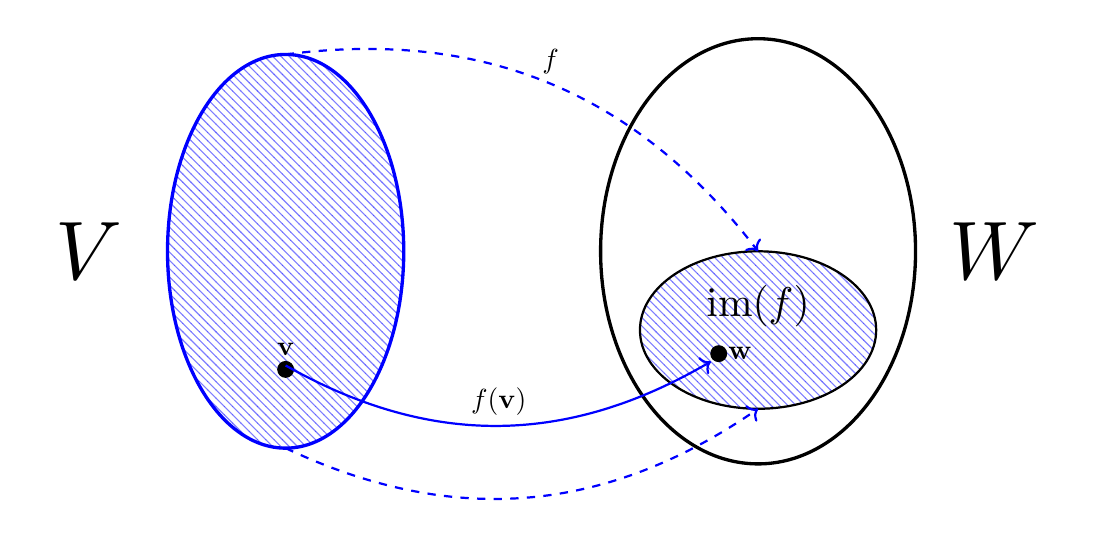
\begin{tikzpicture}
	\coordinate (v) at (0,-1.45);
	\coordinate (w) at (5.5,-1.3);
	
	% domain set V
	\fill[pattern=north west lines, pattern color=blue,opacity=.5,draw] 
  (0,0) ellipse (1.5cm and 2.5cm);
    \draw[very thick,blue] (0,0) ellipse (1.5cm and 2.5cm);
    \node[align=left,scale=3] at (-2.5,0) {$V$};
    \fill[draw] (0,-1.5) circle (0.1cm and 0.1cm);
    \node[above,scale=1] at (v) {$\mathbf{v}$};
    
	% image set f(V) inside W
	\fill[pattern=north west lines, pattern color=blue,opacity=.5,draw] 
  (6,-1) ellipse (1.5cm and 1cm);
    \draw[thick] (6,-1) ellipse (1.5cm and 1cm);
    \node[align=left,scale=1.5] at (6,-0.7) {$\text{im}(f)$};
  
	% codomain set W
    \draw[very thick] (6,0) ellipse (2cm and 2.7cm);
    \node[align=right,scale=3] at (9,0) {$W$};
    \fill[draw] (5.5,-1.3) circle (0.1cm and 0.1cm);
    \node[right,scale=1] at (w) {$\mathbf{w}$};
    
    % mapping lines
	\draw[->, thick, blue, dashed] (0,2.5) to[bend left] node[pos=0.5,above, black,scale=1] {$f$}  (6,0);
	\draw[->, thick, blue, dashed] (0,-2.5) to[bend right] (6,-2);
	\draw[->, thick, blue] (v) to[bend right] node[pos=0.5,above, black,scale=1] {$f(\mathbf{v})$}  ($(w)-(0.1,0.1)$);
\end{tikzpicture}
\end{figure}

\noindent The image is a vector subspace of $W$. Let's prove this. Firstly, we previously showed that any linear map takes the zero vector of $V$ to the zero vector of $W$. So $\mathbf{0}_W \in \text{im}(f)$ and hence it is not an empty set. Let $\mathbf{u}$, $\mathbf{v}\in \text{im}(f)$ and $\alpha$, $\beta \in \mathbb{R}$. There must exist corresponding vectors in $V$, $\mathbf{u}'$ and $\mathbf{v}'$ such that $f(\mathbf{u}')=\mathbf{u}$ and $f(\mathbf{v}')=\mathbf{v}$. Hence
\begin{align*}
\alpha \mathbf{u} + \beta \mathbf{v} = \alpha f(\mathbf{u}') + \beta f(\mathbf{v}') = f(\alpha \mathbf{u}' + \beta \mathbf{v}')
\end{align*}
where we have used the definition of a linear map in the last step. This shows that for any linear combination of vectors in the image of $f$, we can find a corresponding vector in $V$. This means the $\alpha \mathbf{u} + \beta \mathbf{v} \in \text{im}(f)$. Hence the image is a non-empty subset of $W$ that is closed under linear combinations, that is, it is a vector subspace of $W$.

\theorem{Generator of the image}{The image of any linear map, $f:V\to W$, has a generator set that can be found by the action of $f$ on any basis of $V$. That is, let $V$ be an $n$ dimensional vector space and $\mathcal{B}_V=\{\mathbf{b}_1, \dots, \mathbf{b}_n\}$ be a basis of $V$. Then the set $\mathcal{C}=\{f(\mathbf{b}_1),\dots, f(\mathbf{b}_n)\}\subset W$ generates $\text{im}(f)$, that is, 
\begin{align*}
\text{im}(f) = \text{SPAN}\left( f(\mathbf{b}_1),\dots, f(\mathbf{b}_n) \right)
\end{align*}
}

\begin{proof}
Let $\mathbf{w}\in \text{im}(f)$. This means there must exist a $\mathbf{v}\in V$ such that $f(\mathbf{v})=\mathbf{w}$. As $\mathcal{B}_V$ is a basis of $V$, the vector $\mathbf{v}$ can be expressed as a linear combination of the basis vectors
\begin{align*}
\mathbf{v} = \alpha_1 \mathbf{b}_1 + \cdots + \alpha_n \mathbf{b}_n
\end{align*}
hence
\begin{align*}
\mathbf{w} = f(\mathbf{v}) = f(\alpha_1 \mathbf{b}_1 + \cdots + \alpha_n \mathbf{b}_n) = \alpha_1 f(\mathbf{b}_1) + \cdots + \alpha_n f(\mathbf{b}_n).
\end{align*}
This shows that any vector of the image can be expressed as a linear combination of vectors in the set $\mathcal{C}=\{f(\mathbf{b}_1),\dots, f(\mathbf{b}_n)\}$, i.e.
\begin{align*}
\text{im}(f) \subset \text{SPAN}\left( f(\mathbf{b}_1),\dots, f(\mathbf{b}_n) \right).
\end{align*}
The other direction is trivial, but worth the practice. Let $\mathbf{w}\in \text{SPAN}\left( f(\mathbf{b}_1),\dots, f(\mathbf{b}_n) \right)$. This means it can be written as a linear combination of these vectors
\begin{align*}
\mathbf{w} &= \alpha_1 f(\mathbf{b}_1) + \cdots + \alpha_n f(\mathbf{b}_n) \\
&= f(\alpha_1 \mathbf{b}_1 + \cdots + \alpha_n \mathbf{b}_n)
\end{align*}
which means we have found a corresponing vector $\mathbf{v}=\alpha_1 \mathbf{b}_1 + \cdots + \alpha_n \mathbf{b}_n \in V$ such that $f(\mathbf{v}) = \mathbf{w}$. Hence $\mathbf{w}\in \text{im}(f)$. This proves 
\begin{align*}
\text{SPAN}\left( f(\mathbf{b}_1),\dots, f(\mathbf{b}_n) \right) \subset \text{im}(f)
\end{align*}
and so we have the equality of these two sets.
\end{proof}

\definition{Rank}{
The \textit{rank of a linear map} is the dimension of its image: $\text{rank}(f)=\dim(\text{im}(f))$.
}

\example{Rank of a linear map from $\mathbb{R}^3$ to $\mathbb{R}^3$}{Let's find the dimension of a given linear map. Let $f:\mathbb{R}^3 \to \mathbb{R}^3$ be the linear map defined by
\begin{align*}
f(x,y,z) = (x+z, z-y, y-x-2z).
\end{align*}
We take the canonical basis of $\mathbb{R}^3$, $\mathcal{C}=\{\mathbf{e}_1,\mathbf{e}_2,\mathbf{e}_3\}=\{(1,0,0),\, (0,1,0), \, (0,0,1)\}$. From theorem ... we can form the generator set
\begin{align*}
\mathcal{B} &= \{f(\mathbf{e}_1),\, f(\mathbf{e}_2), \, f(\mathbf{e}_3) \} \\
&= \{(1,0,-1), \, (0,-1,1), \, (1,1,-2) \}.
\end{align*}
\noindent Now this set is not a basis, because the third vector is the subtraction of the second from the first (and thus the set $\mathcal{B}$ is not a set of linearly independent vectors). So we can drop the third vector to find
\begin{align*}
\text{im}(f) = \text{SPAN}((1,0,-1), \, (0,-1,1), \, (1,1,-2) ) = \text{SPAN}((1,0,-1), \, (0,-1,1))
\end{align*}
and thus we have the basis of the image
\begin{align*}
\mathcal{C} &= \{(1,0,-1), \, (0,-1,1) \}
\end{align*}
which means the dimension is 2 and hence $\text{rank}(f)=2$.
}

\definition{Kernel}{
The \textit{kernel of a linear map}  $f: V \to W$, denoted $\ker(f)$, is the set of vectors that $f$ maps to the zero vector, $\mathbf{0}_W$, of $W$. That is,
\begin{align*}
\ker(f) = \{\mathbf{v} \in V \,\, | \,\, f(\mathbf{v}) = \mathbf{0}_W \}.
\end{align*}
}

\noindent This can be understood pictorially as so:
\begin{figure}[H]
\centering
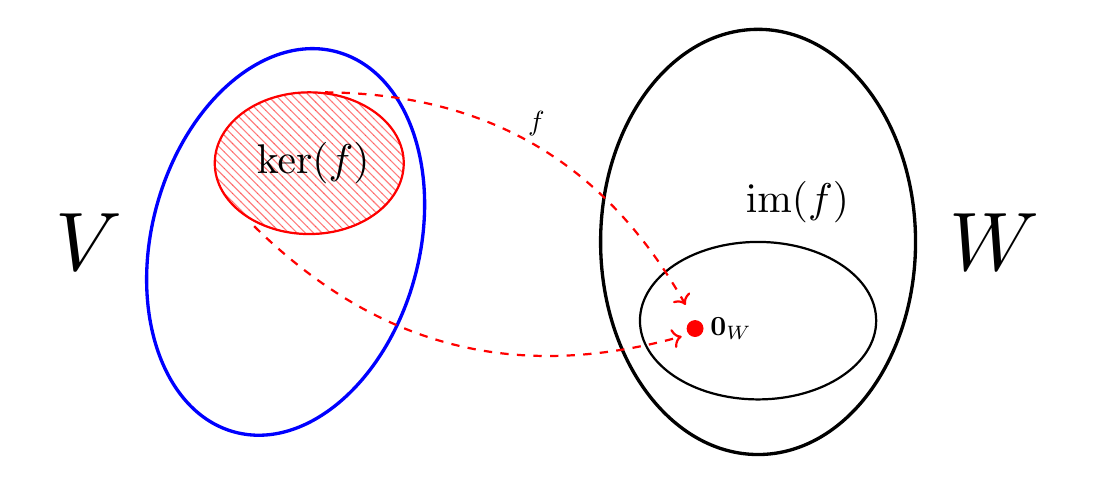
\begin{tikzpicture}
	\coordinate (v) at (0,-1.45);
	\coordinate (Ow) at (5.2,-1.1);
	
	% domain set V
	%\fill[pattern=north west lines, pattern color=blue,opacity=.5,draw] 
		%(0,0) ellipse (1.5cm and 2.5cm);
    \draw[very thick,blue,rotate around={-15:(0,0)}] (0,0) ellipse (1.7cm and 2.5cm);
    \node[align=left,scale=3] at (-2.5,0) {$V$};
    %\fill[draw] (0,-1.5) circle (0.1cm and 0.1cm);
    %\node[above,scale=1] at (v) {$\mathbf{v}$};
  
	% codomain set W
    \draw[very thick] (6,0) ellipse (2cm and 2.7cm);
    \node[align=right,scale=3] at (9,0) {$W$};
    
	% kernel set ker(f) inside V
	\fill[pattern=north west lines, pattern color=red,opacity=.5,draw] 
  		(0.3,1) ellipse (1.2cm and 0.9cm);
    \draw[thick,red] (0.3,1) ellipse (1.2cm and 0.9cm);
    \node[align=left,scale=1.5] at (0.35,1) {$\ker(f)$};
    
	% image set f(V) inside W
    \draw[thick] (6,-1) ellipse (1.5cm and 1cm);
    \node[align=left,scale=1.5] at (6.5,0.5) {$\text{im}(f)$};
    
    % zero vector in W
    \fill[draw,red] (Ow) circle (0.1cm and 0.1cm);
    \node[right=2pt,scale=1] at (Ow) {$\mathbf{0}_W$};
    
    % mapping lines
	\draw[->, thick, red, dashed] (0.5,1.9) to[bend left] node[pos=0.5,above, black,scale=1] {$f$}  ($(Ow)+(-0.12,0.3)$);
	\draw[->, thick, red, dashed] (-0.4,0.2) to[bend right] ($(Ow)+(-0.17,-0.1)$);
\end{tikzpicture}
\end{figure}



\example{Kernel of a linear map from $\mathbb{R}^3$ to $\mathbb{R}^3$}{Let's find the kernel of the linear map from the previous example, the map $f:\mathbb{R}^3 \to \mathbb{R}^3$ defined by
\begin{align*}
f(x,y,z) = (x+z, z-y, y-x-2z).
\end{align*}
We want to find all the triples that $f$ takes to the zero vector of $\mathbb{R}^3$, which is $(0,0,0)$. Hence we are looking to solve
\begin{align*}
f(x,y,z)=(0,0,0) \quad \implies \quad (x+z, z-y, y-x-2z) = (0,0,0).
\end{align*}
Equating components gives us the linear system
\begin{align*}
\begin{cases}
x+z = 0 \\
z-y=0 \\ 
y-x-2z =0
\end{cases}
%
\quad \implies \quad
%
\begin{cases}
x = -z \\
y=z \\ 
y-x-2z =0
\end{cases}.
\end{align*}
So $x$ and $y$ can each be expressed in terms of $z$ and the 3rd equation gives no extra constraint. $z$ is therefore a free variable, denote it $z=t\in\mathbb{R}$, and we have
\begin{align*}
f(x,y,z) = (0,0,0)\quad \implies \quad (x,y,z)=(-t,t,t)=(-1,1,1)t.
\end{align*}
So we can write the kernel as the set
\begin{align*}
\ker(f) = \{(-1,1,1)t \, | \, t\in\mathbb{R} \}.
\end{align*}
}

\noindent The kernel is a vector subspace of $W$. It is non-empty because the zero vector necessarily maps to the zero, $f(\mathbf{0}_V)=\mathbf{0}_W$, and so $\mathbf{0}_V\in \ker(f)$. Let $\mathbf{u},\mathbf{v}\in \ker(f)$ and $\alpha,\beta \in\mathbb{R}$. Then $f$ maps the linear combination as
\begin{align*}
f( \alpha \mathbf{u} + \beta \mathbf{v}) =  \alpha f(\mathbf{u}) + \beta f(\mathbf{v}) = \alpha \mathbf{0}_W + \beta \mathbf{0}_W = \mathbf{0}_W
\end{align*}
and so $\alpha \mathbf{u} + \beta \mathbf{v}$ is also in the kernel of $f$. Thus $\ker(f)$ is closed under linear combinations and is a non-empty subset of $V$. Therefore it is a vector subspace of $V$.

\definition{Nullity}{
The \textit{nullity of a linear map} is the dimension of its kernel: $\text{nullity}(f)=\dim(\ker(f))$.
}





\example{Nullity of a linear map from $\mathbb{R}^3$ to $\mathbb{R}^3$}{Let's retake the linear map from the previous example, $f:\mathbb{R}^3 \to \mathbb{R}^3$ defined by
\begin{align*}
f(x,y,z) = (x+z, z-y, y-x-2z).
\end{align*}
We found the kernel as the set
\begin{align*}
\ker(f) = \{(-1,1,1)t \, | \, t\in\mathbb{R} \} = \text{SPAN}( \, (-1,1,1) \, ).
\end{align*}
This means that the set $\mathcal{B} = \{ (-1,1,1) \}$ is a basis for the kernel. Hence the dimension of kernel is 1, and so
\begin{align*}
\text{nullity}(f) = \dim(\ker(f)) = 1.
\end{align*}
}

\theorem{Rank-Nullity}{
For any linear map $f: V \to W$ we have
\begin{gather*}
\text{rank}(f) + \text{nullity}(f) = \dim(V) \\
\text{or} \\
\dim(\text{im}(f)) + \dim(\ker(f)) = \dim(V). 
\end{gather*}
}

\example{Projection map onto the $x$-$y$ plane}{
Consider the linear map $f:\mathbb{R}^3 \to \mathbb{R}^3$ defined by
\begin{align*}
f(x,y,z) = (x,y,0).
\end{align*}
This map takes any vector in 3d space and gives you the component of that vector in the $x$-$y$ plane. Here's a sketch of the action of $f$ on a couple of example vectors

\begin{figure}[H]
\centering
\tdplotsetmaincoords{105}{-30}
\begin{tikzpicture}[tdplot_main_coords,font=\sffamily]
  \begin{scope}[canvas is xy plane at z=0]
    \fill[blue,fill opacity=0.1] (-3,-3) rectangle (3,4); 
   
   \pgflowlevelsynccm
  \end{scope}
    
  \coordinate (O) at (0,0);
  \coordinate (u) at (2,5,2);
  \coordinate (fu) at (2,5,0);
  \coordinate (v) at (3,-1,2);
  \coordinate (fv) at (3,-1,0);
  \draw [->,red,thick] (O) --(u) node[pos=0.6,below=1pt] {$\mathbf{u}$};
  \draw [->,blue,dashed,thick] (O) --(fu) node[pos=0.6,right=1pt] {$f(\mathbf{u})$};
  \draw [-,black,dashed] ($0.1*(fu)+0.9*(u)$) --($0.8*(fu)+0.2*(u)$);
  
  
  \draw [->,red,thick] (O) --(v) node[pos=0.6,above=1pt] {$\mathbf{v}$};
  \draw [->,blue,dashed,thick] (O) --(fv) node[pos=0.6,above=1pt] {$f(\mathbf{v})$};
  \draw [-,black,dashed] ($0.1*(fv)+0.9*(v)$) --($0.9*(fv)+0.1*(v)$);
    
  \pgfmathsetmacro{\Radius}{1.5}
  \draw[-stealth] (O)-- (2.5*\Radius,0,0) node[pos=1.15] {$y$};
  \draw[-stealth] (O) -- (0,3.5*\Radius,0) node[pos=1.15] {$x$};
  \draw[-stealth] (O) -- (0,0,2*\Radius) node[pos=1.05] {$z$};
\end{tikzpicture}
\end{figure}

\noindent Now the image of this function is clearly all of the $x$-$y$ plane, but let's show that mathematically. Take the canonical basis of $\mathbb{R}^3$: $\mathcal{C}=\{\mathbf{e}_1,\mathbf{e}_2,\mathbf{e}_3\}=\{(1,0,0),\, (0,1,0), \, (0,0,1)\}$. We have the generator set
\begin{align*}
\mathcal{B} &= \{f(\mathbf{e}_1),\, f(\mathbf{e}_2), \, f(\mathbf{e}_3) \} \\
&= \{(1,0,0), \, (0,1,0), \, (0,0,0) \}.
\end{align*}
The span of this set is the same as if we drop the zero vector, so
\begin{align*}
\mathcal{C} = \{(1,0,0), \, (0,1,0) \}
\end{align*}
is a set of linearly independent vectors such that $\text{im}(f)=\text{SPAN}(\mathcal{C})$, which means $\mathcal{C}$ is a basis for the image. With two vectors in this basis, we have the dimension of the image, and therefore the rank of $f$, is 2.

Now for the kernel we must solve
\begin{align*}
f(x,y,z)=(0,0,0).
\end{align*}
This gives us $(x,y,0) = (0,0,0)$ so that $x=0$ and $y=0$. There is no restriction on $z$, so that the kernel can be written as the set
\begin{align*}
\ker(f) = \{ (0,0,1)t \, | \, t\in\mathbb{R}\} = \text{SPAN}((0,0,1)).
\end{align*}
So we can form the obvious basis $\mathcal{D}=\{ (0,0,1) \}$, showing the dimension of the kernel, and hence the nullity of $f$, is 1. We thus verify that for this linear map, we have $\text{rank}(f) + \text{nullity}(f) = 2 + 1 = 3 = \dim(\mathbb{R}^3)$.
}

\definition{Injectivity}{
Let $f:V\to W$ be a linear map. We say $f$ is injective if no two vectors of $V$ are mapped to the same vector of $W$. In symbols we have two equivalent expressions
\begin{gather*}
\forall \, \mathbf{x},\mathbf{y}\in V, \quad \left(f(\mathbf{x})=f(\mathbf{y}) \implies \mathbf{x}=\mathbf{y}\right) \\
%
\text{or} \\
%
\forall \, \mathbf{x},\mathbf{y}\in V, \quad \left( \mathbf{x} \neq \mathbf{y} \implies f(\mathbf{x}) \neq f(\mathbf{y})\right)  
\end{gather*}
}

\definition{Surjectivity}{
Let $f:V\to W$ be a linear map. We say that $f$ is surjective if every vector in the output space has a corresponding input vector. In symbols
\begin{align*}
\forall \, \mathbf{w} \in W \quad \exists \mathbf{v}\in V \, \text{such that} \, f(\mathbf{v})=\mathbf{w}.
\end{align*}
}

\definition{Categories of linear maps}{
Let $f:V\to W$ be a linear map.
\begin{itemize}
\item If $W=V$ we call $f$ an \textit{endomorphism}.
\item If $f$ is both injective and surjective then we say it is bijective and we call it an \textit{isomorphism}.
\item If $f$ is both an isomorphism and an endomorphism we call it an \textit{automorphism}.
\end{itemize}
}

\definition{Composition of linear maps}{
Composition of linear maps works exactly as you would expect if you remember the composition of regular functions. We must have a coherence between the output of one linear map and the input of another. So, two linear maps $f:A\to B$ and $g:U\to V$ can be composed as a well defined linear map $g\circ f$ (``$g$ of $f$'') if and only if the output space of $f$ is the input space of $g$: $U=B$. For any $\mathbf{u}\in A$ the composition is written
\begin{align*}
g\circ f: A \to V \quad \text{and} \quad (g\circ f)(\mathbf{u}) = g(f(\mathbf{u})).
\end{align*}
}

\noindent The composition can be represented pictorially as so:
\begin{figure}[H]
\centering
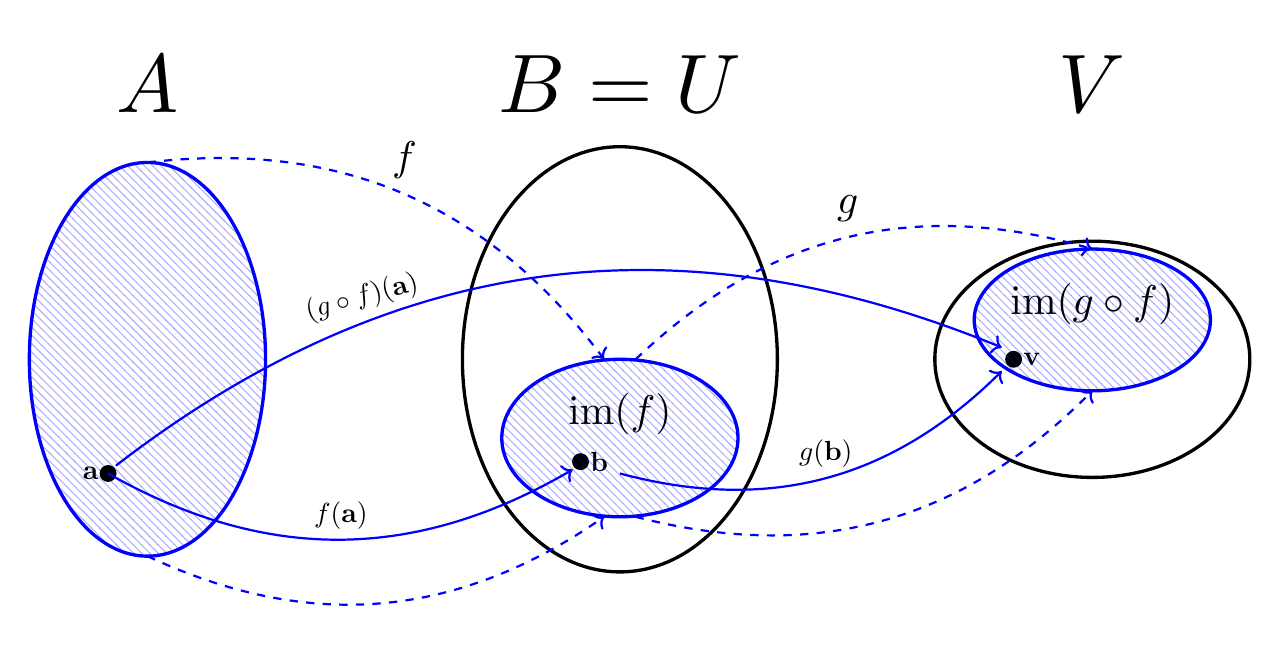
\begin{tikzpicture}
	\coordinate (a) at (-0.5,-1.45);
	\coordinate (b) at (5.5,-1.3);
	\coordinate (v) at (11,0);
	
	% domain set A
	\fill[pattern=north west lines, pattern color=blue,opacity=.3,draw] 
  (0,0) ellipse (1.5cm and 2.5cm);
    \draw[very thick,blue] (0,0) ellipse (1.5cm and 2.5cm);
    \node[align=center,scale=3] at (0,3.5) {$A$};
    \fill[draw] (a) circle (0.1cm and 0.1cm);
    \node[left,scale=1] at (a) {$\mathbf{a}$};
  
	% codomain set B=U
    \draw[very thick] (6,0) ellipse (2cm and 2.7cm);
    \node[align=center,scale=3] at (6,3.5) {$B=U$};
    \fill[draw] (b) circle (0.1cm and 0.1cm);
    \node[right,scale=1] at (b) {$\mathbf{b}$};
  
	% codomain set V
    \draw[very thick] (12,0) ellipse (2cm and 1.5cm);
    \node[align=center,scale=3] at (12,3.5) {$V$};
    \fill[draw] (v) circle (0.1cm and 0.1cm);
    \node[right,scale=1] at (v) {$\mathbf{v}$};
    
	% image set g(A) inside B
	\fill[pattern=north west lines, pattern color=blue,opacity=.3,draw] 
  (6,-1) ellipse (1.5cm and 1cm);
    \draw[very thick,blue] (6,-1) ellipse (1.5cm and 1cm);
    \node[align=left,scale=1.5] at (6,-0.7) {$\text{im}(f)$};
  
	% iamge set f(g(A))
	\fill[pattern=north west lines, pattern color=blue,opacity=.3,draw] 
  (12,0.5) ellipse (1.5cm and 0.9cm);
    \draw[very thick,blue] (12,0.5) ellipse (1.5cm and 0.9cm);
    \node[align=left,scale=1.5] at (12,0.7) {$\text{im}(g\circ f)$};
    
    % mapping lines
    % A to B
	\draw[->, thick, blue, dashed] (0,2.5) to[bend left] node[pos=0.5,above, black,scale=1.5] {$f$}  (5.8,0);
	\draw[->, thick, blue, dashed] (0,-2.5) to[bend right] (5.8,-2);
	
    % B to V
	\draw[->, thick, blue, dashed] (6.2,0) to[bend left] node[pos=0.5,above, black,scale=1.5] {$g$}  (12,1.4);
	\draw[->, thick, blue, dashed] (6.2,-2) to[bend right] (12,-0.4);
	
	% example functions f(a)=b, g(b)=v, and g(f(a))=v
	\draw[->, thick, blue] (a) to[bend right] node[pos=0.5,above, black,scale=1] {$f(\mathbf{a})$}  ($(b)-(0.1,0.1)$);
	\draw[->, thick, blue] ($(b)+(0.5,-0.15)$) to[bend right]
	 node[pos=0.5,above, black,scale=1] {$g(\mathbf{b})$}  ($(v)-(0.15,0.15)$);
	\draw[->, thick, blue] ($(a)+(0.1,0.1)$) to[bend left]
	 node[pos=0.3,above,rotate=15,black,scale=1] {$(g\circ f)(\mathbf{a})$}  ($(v)+(-0.15,0.15)$);
\end{tikzpicture}
\end{figure}


\example{Composition of linear maps}{
Let's come up with a couple of linear maps and then take their composition, why not? Consider $f:\mathbb{R}^2 \to \mathcal{P}_3[\mathbb{R}]$ and $g: \mathcal{P}_3[\mathbb{R}]\to \mathbb{R}^3$ defined by
\begin{align*}
& f(\alpha,\beta) = \alpha + (\beta-\alpha)x + (\alpha + 2\beta)x^3 \\
& g(a_0 + a_1 x + a_2 x^2 + a_3 x^3) = (a_3, \, a_2-a_1, \, a_0+a_3).
\end{align*}
Now the composition of these linear maps will skip the polynomial space (the output of $f$ and input of $g$):
\begin{align*}
g \circ f: & \mathbb{R}^2 \to \mathbb{R}^3 \\
(g \circ f)(\alpha,\beta) & = g \left(f(\alpha,\beta)\right) \\
 & = g \left(\alpha + (\beta-\alpha)x + (\alpha + 2\beta)x^3\right) \\
 & = (\alpha + 2\beta, \, \alpha-\beta, \, 2\alpha + 2\beta)
\end{align*}
So let's see for example what happens to the vector $\mathbf{v}=(1,1)$. If we consider the step-by-step process, first act with $f$ to obtain a polynomial, then hit that polynomial with $g$, we find
\begin{align*}
f(\mathbf{v}) & = f(1,1) = 1 + 3x^3 \\
\implies g(f(\mathbf{v})) &= g(1+3x^3) = \left(3, \, 0, \, 4 \right).
\end{align*}
If we want to avoid this 2-step process we can use the composition rule as we found above
\begin{align*}
(g \circ f)(1,1) = (1 + 2, \, 1-1, \, 2 + 2) = (3, \, 0, \, 4).
\end{align*}
Of course we get the same answer, but the lesson here is that we never had to think about polynomials this way.
}



\theorem{Inverse linear map}{
Let $f:V\to W$ be a linear map. If $f$ is bijective then there exists a linear map $g:W\to V$ such that
\begin{gather*}
\forall \, \mathbf{v}\in V \, \text{we have} \, (g \circ f)(\mathbf{v}) = \mathbf{v}\\
\text{and}\\
\forall \, \mathbf{w}\in W \, \text{we have} \, (f \circ g)(\mathbf{w}) = \mathbf{w}
\end{gather*}
$g$ is called the inverse of $f$ and is denoted $f^{-1}$.
}

\section{The vector space of linear maps}


\theorem{The set of linear maps as a vector space}{
Consider the set of all possible linear maps from the vector space $V$ to the vector space $W$, denoted $\mathcal{L}(V,W)$. This set satisfies all of the vector space axioms if we define vector addition and scalar multiplication as follows:
\begin{gather*}
\forall f,g \in \mathcal{L}(V,W), \quad f+g=h \quad \text{such that} \quad h(\mathbf{v})=f(\mathbf{v}) + g(\mathbf{v}) \\
\text{and} \\
\forall \alpha \in \mathbb{R}\, \quad \alpha f = f_\alpha \quad \text{such that} \quad f_\alpha(\mathbf{v})=\alpha \left( f(\mathbf{v}) \right).
\end{gather*}
}

\noindent \textbf{Proof}. Let $f,g,h\in \mathcal{L}(V,W)$ and $\alpha,\beta\in\mathbb{R}$. Let's go through the vector space axioms in order:

\noindent \underline{VA1 - closure under vector addition: $f+g\in \mathcal{L}(V,W)$} \\
\noindent Let the addition be denoted $h = f+g$. We have to show that $h$ is a linear map from $V$ to $W$. For every $\mathbf{v},\mathbf{u}\in V$ and $\alpha,\beta\in\mathbb{R}$ we have
\begin{align*}
h(\alpha\mathbf{v} + \beta\mathbf{u}) &= f(\alpha\mathbf{v} + \beta\mathbf{u}) + g(\alpha\mathbf{v} + \beta\mathbf{u}) \\
%
&= \alpha f(\mathbf{v}) + \beta f (\mathbf{u}) + \alpha g(\mathbf{v}) + \beta g(\mathbf{u}) \quad \text{(because $f$ and $g$ are linear maps)}\\
%
&= \alpha \left( f(\mathbf{v}) + g(\mathbf{v})\right)  + \beta\left( f (\mathbf{u})+ g(\mathbf{u})\right) \\
%
&= \alpha h(\mathbf{v}) + \beta h(\mathbf{u}).
\end{align*}
So $f+g$ preserves linear combinations and is therefore a linear map. Hence $\mathcal{L}(V,W)$ is closed under vector addition. \\
%%%%%%%


%%%%%%%
\noindent \underline{VA2 - associativity of vector addition: $f+(g+h) = (f+g)+h \in \mathcal{L}(V,W)$}

\noindent For every $\mathbf{v}\in V$ we have
\begin{align*}
(f+(g+h))(\mathbf{v}) &= f(\mathbf{v})+(g+h)(\mathbf{v})  &  (\text{definition of vector addition of linear maps})\\
 &= f(\mathbf{v})+(g(\mathbf{v})+h(\mathbf{v}) )   &  (\text{definition of vector addition of linear maps})\\
 &= (f(\mathbf{v})+g(\mathbf{v}))+h(\mathbf{v})    &  (\text{associativity of vectors in $W$})\\
 &= (f+g)(\mathbf{v})+h(\mathbf{v})    &  (\text{definition of vector addition of linear maps})\\
 &= ((f+g)+h)(\mathbf{v})    &  (\text{definition of vector addition of linear maps}).
\end{align*}
This shows that $f+(g+h)$ is the same linear map as $(f+g)+h$. Hence the addition of vectors in $\mathcal{L}(V,W)$ is associative. \\
%%%%%%%


%%%%%%%
\noindent \underline{VA3 - additive identity: $\exists \, f_0 \in \mathcal{L}(V,W), \, \text{such that} \, f + f_0 = f_0 + f = f$}

\noindent Define the zero map $f_0: V \to W$ by
\begin{align*}
f_0(\mathbf{v}) = \mathbf{0}_W
\end{align*}
for every $\mathbf{v}\in V$. Firstly, is this a linear map? Let's see if it preserves linear combinations
\begin{align*}
f_0(\alpha \mathbf{v} + \beta \mathbf{u}) &= \mathbf{0}_W  &  (\text{definition of the zero map}) \\
%
 &= \mathbf{0}_W + \mathbf{0}_W  &  (\text{definition of the zero vector of $W$}) \\
%
 &= \alpha \mathbf{0}_W + \beta\mathbf{0}_W  &  (\text{a number multiplied by the zero vector is the zero vector})  \\
%
 &= \alpha f_0(\mathbf{v}) + \beta f_0(\mathbf{u})  &  (\text{reverse definition of the zero map}) .
\end{align*}
Indeed, this zero map is a linear map from $V$ to $W$, that is $f_0 \in \mathcal{L}(V,W)$. Now we must show that this map acts as the zero vector of $\mathcal{L}(V,W)$. For every $\mathbf{v}\in V$ we have
\begin{align*}
(f_0 + f)(\mathbf{v}) &= f_0(\mathbf{v})+f(\mathbf{v})  &  (\text{definition of vector addition of linear maps})\\
%
&= \mathbf{0}_W+f(\mathbf{v})  &  (\text{definition of zero map})\\
%
&= f(\mathbf{v})+\mathbf{0}_W  &  (\text{commutativity of vector addition in $W$})\\
%
&= f(\mathbf{v})  &  (\text{definition of zero vector of $W$})
\end{align*}
Hence this zero map is a member of $\mathcal{L}(V,W)$ and satisifes $f + f_0 = f_0 + f = f$. This proves the zero map is the zero \textit{vector} of $\mathcal{L}(V,W)$. \\
%%%%%%%


%%%%%%%
\noindent \underline{VA4 - additive inverse: $\exists \, f_- \in \mathcal{L}(V,W) \, \text{such that} \, f + f_- = f_0$}

\noindent This can easily become symbolically ambiguous, so I will try to be pedantically careful here. Define the additive inverse of any map $f$, denote it $f_-$, as the scalar multiplication of that map (as defined) by the real number $-1$. So that the map $f_-:V\to W$ is given by
\begin{align*}
f_-(\mathbf{v}) = -1 \times f(\mathbf{v}).
\end{align*}
First let's show this map belongs to $\mathcal{L}(V,W)$ by checking the preservation of linear combinations
\begin{align*}
f_-(\alpha \mathbf{v} + \beta \mathbf{u}) &= -1\times f(\alpha \mathbf{v} + \beta \mathbf{u})  &  (\text{definition of this map}) \\
%
 &= -1\times \left( \alpha f(\mathbf{v)} + \beta f(\mathbf{u}) \right)  &  (\text{linearity of the map $f$}) \\
%
 &= -1\times \alpha f(\mathbf{v)} -1\times \beta f(\mathbf{u})  &  (\text{distributivity of the reals}) \\
%
 &= \alpha \times -1\times f(\mathbf{v)} + \beta \times -1\times f(\mathbf{u})  &  (\text{commutativity of real multiplication}) \\
%
 &= \alpha f_-(\mathbf{v)} + \beta f_-(\mathbf{u})  &  (\text{definition of this map}).
\end{align*}
Indeed, this map is a linear map from $V$ to $W$, that is $f_- \in \mathcal{L}(V,W)$. Now we show that it acts as an additive inverse. For every $\mathbf{v}\in V$ we have
\begin{align*}
(f_- + f)(\mathbf{v}) &= f_-(\mathbf{v}) + f(\mathbf{v})  &  (\text{definition of vector addition of linear maps}) \\
%
 &= -1\times f(\mathbf{v}) + f(\mathbf{v})  &  (\text{definition of this map}) \\
%
 &= -f(\mathbf{v}) + f(\mathbf{v})  &  (\text{multiplication by 1 for vectors in $W$}) \\
%
 &= \mathbf{0}_W  &  (\text{additive inverse of vectors in $W$})
\end{align*}
With commutativity of vectors in $W$ you can also show $f_- + f = f + f_-$. Hence this additive inverse map exists in $\mathcal{L}(V,W)$.
\\
%%%%%%%


%%%%%%%
\noindent \underline{VA5 - commutativity of vector addition: $f + g  = g + f$}

\noindent This one is pretty simple. For every $\mathbf{v}\in V$ we have
\begin{align*}
(f + g)(\mathbf{v}) &= f(\mathbf{v}) + g(\mathbf{v})  &  (\text{definition of vector addition of linear maps}) \\
%
&= g(\mathbf{v}) + f(\mathbf{v})  &  (\text{commutativity of vector addition in $W$}) \\
%
&= (g+ f)(\mathbf{v})  &  (\text{definition of vector addition of linear maps}).
\end{align*}
Hence the addition of vectors in $\mathcal{L}(V,W)$ is commutative. \\
%%%%%%%


%%%%%%%
\noindent \underline{SM1 - closure under scalar multiplication: $\alpha f \in \mathcal{L}(V,W)$}

\noindent Recall the definition of scalar multiplication of the linear map $f$ by a real number $k$ gives a new map, denote it $f_k$, such that
\begin{align*}
f_k(\mathbf{v}) = k f(\mathbf{v}).
\end{align*}
Let's show this map belongs to $\mathcal{L}(V,W)$ by checking the preservation of linear combinations
\begin{align*}
f_k(\alpha \mathbf{v} + \beta \mathbf{u}) &= k f(\alpha \mathbf{v} + \beta \mathbf{u})  &  (\text{definition of this map}) \\
%
 &= k \left( \alpha f(\mathbf{v)} + \beta f(\mathbf{u}) \right)  &  (\text{linearity of the map $f$}) \\
%
 &= k \alpha f(\mathbf{v)} +k \beta f(\mathbf{u})  &  (\text{distributivity of the reals}) \\
%
 &= \alpha \times kf(\mathbf{v)} + \beta \times kf(\mathbf{u})  &  (\text{commutativity of real multiplication}) \\
%
 &= \alpha f_k(\mathbf{v)} + \beta f_k(\mathbf{u})  &  (\text{definition of this map}).
\end{align*}
Indeed, this map is a linear map from $V$ to $W$, and so $\mathcal{L}(V,W)$ is closed under scalar multiplication. \\
%%%%%%%


%%%%%%%
\noindent \underline{SM2 - distributivity over vector addition: $\alpha(f+g)=\alpha f+\alpha g$}

\noindent For every $\mathbf{v}\in V$ we have
\begin{align*}
(\alpha(f+g)) (\mathbf{v}) &= \alpha((f+g) (\mathbf{v}))  &  (\text{definition of scalar multiplication for linear maps}) \\
%
&=  \alpha(f(\mathbf{v})+g(\mathbf{v})) &  (\text{definition of vector addition for linear maps}) \\
%
&=  \alpha \left(f(\mathbf{v})\right) +\alpha \left( g(\mathbf{v})\right)  &  (\text{distributivity over vector addition in $W$})\\
%
&=  \left(\alpha f\right)(\mathbf{v}) +\left(\alpha  g\right)(\mathbf{v})  &  (\text{definition of scalar multiplication for linear maps})\\
%
&=  \left(\alpha f + \alpha  g\right)(\mathbf{v})  &  (\text{definition of addition  for linear maps}).
\end{align*}
This shows that $\alpha(f+g)$ is the same linear map as $\alpha f+\alpha g$. Hence scalar multiplication for linear maps distributes over vector addition of linear maps. \\
%%%%%%%


%%%%%%%
\noindent \underline{SM3 - distributivity with field addition: $(\alpha+\beta)f=\alpha f+\beta g$}

\noindent For every $\mathbf{v}\in V$ we have
\begin{align*}
\left( (\alpha+\beta)f \right)(\mathbf{v}) &= (\alpha+\beta)\left( f(\mathbf{v}) \right) 
 & (\text{definition of scalar multiplication for linear maps}) \\
%
 &= \alpha  f(\mathbf{v}) +\beta  f(\mathbf{v})
 & (\text{distributivity over field addition for $W$}) \\
%
 &= \left(\alpha f\right)(\mathbf{v}) + \left(\beta f\right) (\mathbf{v})
 & (\text{definition of scalar multiplication for linear maps}) \\
%
 &= \left(\alpha f + \beta f\right) (\mathbf{v})
 & (\text{definition of vector addition for linear maps}).
\end{align*}
This shows that $(\alpha+\beta)f$ is the same linear map as $\alpha f + \beta f$. Hence field addition distributes over linear maps. 
\\
%%%%%%%


%%%%%%%
\noindent \underline{SM4 - compatibility of scalar and field multiplication: $\alpha(\beta f)=(\alpha\beta) f$}

\noindent For every $\mathbf{v}\in V$ we have
\begin{align*}
\left( \alpha(\beta f) \right)(\mathbf{v}) &= \alpha\left( (\beta f) (\mathbf{v}) \right)
 & (\text{definition of scalar multiplication for linear maps}) \\
%
 &= \alpha\left( \beta (f (\mathbf{v}))  \right)
 & (\text{definition of scalar multiplication for linear maps}) \\
%
 &= \left(\alpha \beta \right)(f (\mathbf{v}))
 & (\text{compatibility of scalar and field multiplication for $W$}) \\
%
 &= \left(\left( \alpha \beta \right)f \right) (\mathbf{v})
 & (\text{definition of scalar multiplication for linear maps})
\end{align*}
This shows that $\alpha(\beta f)$ is the same linear map as $(\alpha\beta) f$. Hence scalar multiplication is compatible with field multiplication for linear maps. 
\\
%%%%%%%


%%%%%%%
\noindent \underline{SM5 - multiplicative identity: $1f=f$}

\noindent For every $\mathbf{v}\in V$ we have
\begin{align*}
\left(1 f \right)(\mathbf{v}) &= 1\left( f(\mathbf{v}) \right)
 & (\text{definition of scalar multiplication for linear maps}) \\
%
 &= f (\mathbf{v})
 & (\text{multiplicative identity for $W$})
\end{align*}
This shows that $1f$ is the same linear map as $f$. Hence the real number $1$ is the scalar multiplicative identity for linear maps. \vspace{0.5cm} \\
\noindent It was long and perhaps tedious but we have now completed the proof that with this definition of linear map vector addition and scalar multiplication, the set $\mathcal{L}(V,W)$ satisfies all 10 of the vector space axioms.






%%%%%%%%%%%%%%%%%%%%
%%%%%%%%%%%%%%%%%%%%
%%%%%%%%%%%%%%%%%%%%
\section{Linear maps as matrices}

Let's recall the definition of coordinates of a vector. Given any vector $\mathbf{v}$ in some $n$-dimensional vector space $V$, if we have a basis $\mathcal{B}=\{ \mathbf{b}_1, \dots, \mathbf{b}_n \}$ then the coordinates of $\mathbf{v}$ \textit{in this basis}, denoted $[\mathbf{v}]_\mathcal{B}$, is a column of $n$ numbers which are the coefficients of the linear combination of $\mathbf{v}$ in the basis vectors
\begin{align*}
\mathbf{v}=\alpha_1 \mathbf{b}_1 + \cdots + \alpha_n \mathbf{b}_n \quad\implies\quad [\mathbf{v}]_\mathcal{B} = \begin{pmatrix} \alpha_1 \\ \vdots \\ \alpha_n \end{pmatrix}.
\end{align*}

\noindent I hope to show in this section something quite powerful about linear algebra, that any $n$-dimensional vector space can be mapped to $\mathbb{R}^n$, via the coordinates, and that linear maps take on a particularly simple to use form when mapping between coordinates. We'll start by an example.

\example{Rotation linear map}{
Let's retake the first example of this chapter, the linear map, $f:\mathbb{R}^2 \to \mathbb{R}^2$, that rotates 2d vectors by $45^\circ$ anti-clockwise, defined in detail by
\begin{align*}
f(x,y) = \frac{1}{\sqrt{2}} \left(x-y, x+y \right).
\end{align*}
Let $\mathcal{C}=\{\mathbf{e}_x, \, \mathbf{e}_y\} = \{(1,0), \, (0,1)\}$. We will want to represent $f$ by some operation, call it $F$, that takes the coordinates of any vector to the coordinates of the rotated vector. Let's write this desired property as
\begin{align*}
F[\mathbf{v}]_\mathcal{C} = [f(\mathbf{v})]_\mathcal{C}.
\end{align*}
Now let $\mathbf{v}=(x,y)$ be some arbitrary vector, so that 
\begin{align*}
[f(\mathbf{v})]_\mathcal{C} &= [f(x\mathbf{e}_x + y \mathbf{e}_y)]_\mathcal{C} \\
%
 &= [ \frac{1}{\sqrt{2}} \left(x-y, x+y \right)]_\mathcal{C} \\
%
 &= [\left(\frac{x - y}{\sqrt{2}}\right)\mathbf{e}_x + \left(\frac{x + y}{\sqrt{2}}\right)\mathbf{e}_y]_\mathcal{C} \\
%
 &= \begin{pmatrix}
 \dfrac{x - y}{\sqrt{2}} \\ \dfrac{x + y}{\sqrt{2}}
 \end{pmatrix}.
\end{align*}
These coordinates can be rearranged to focus on the $x$ and $y$
\begin{align*}
\begin{pmatrix}
 \dfrac{x - y}{\sqrt{2}} \\ \dfrac{x + y}{\sqrt{2}}
\end{pmatrix}
%
=
%
\begin{pmatrix}
 \dfrac{x}{\sqrt{2}} \\ \dfrac{x}{\sqrt{2}}
\end{pmatrix}
+
\begin{pmatrix}
 \dfrac{- y}{\sqrt{2}} \\ \dfrac{y}{\sqrt{2}}
\end{pmatrix}
%
=
%
\begin{pmatrix}
 \dfrac{1}{\sqrt{2}} \\ \dfrac{1}{\sqrt{2}}
\end{pmatrix}x
+
\begin{pmatrix}
 \dfrac{-1}{\sqrt{2}} \\ \dfrac{1}{\sqrt{2}}
\end{pmatrix}y.
\end{align*}
So at this point we have
\begin{align*}
F[\mathbf{v}]_\mathcal{C} = [f(\mathbf{v})]_\mathcal{C} \quad\implies\quad 
F
\begin{pmatrix}
 x \\ y
\end{pmatrix}
%
=
%
\begin{pmatrix}
 \dfrac{1}{\sqrt{2}} \\ \dfrac{1}{\sqrt{2}}
\end{pmatrix}x
+
\begin{pmatrix}
 \dfrac{-1}{\sqrt{2}} \\ \dfrac{1}{\sqrt{2}}
\end{pmatrix}y.
\end{align*}
We will define a certain rearrangement of the right hand side
\begin{align*}
\begin{pmatrix}
 \dfrac{1}{\sqrt{2}} \\ \dfrac{1}{\sqrt{2}}
\end{pmatrix}x
+
\begin{pmatrix}
 \dfrac{-1}{\sqrt{2}} \\ \dfrac{1}{\sqrt{2}}
\end{pmatrix}y
=
\begin{pmatrix}
 \dfrac{1}{\sqrt{2}} & \dfrac{-1}{\sqrt{2}} \\ 
 \dfrac{1}{\sqrt{2}} & \dfrac{1}{\sqrt{2}}
\end{pmatrix}
\begin{pmatrix}
 x \\ y
\end{pmatrix}
\end{align*}
so that the equation
\begin{align*}
F
\begin{pmatrix}
 x \\ y
\end{pmatrix}
%
=
%
\begin{pmatrix}
 \dfrac{1}{\sqrt{2}} & \dfrac{-1}{\sqrt{2}} \\ 
 \dfrac{1}{\sqrt{2}} & \dfrac{1}{\sqrt{2}}
\end{pmatrix}
\begin{pmatrix}
 x \\ y
\end{pmatrix}
\end{align*}
lets us identify the operation of $F$ with this array of 4 numbers
\begin{align*}
F
%
=
%
\begin{pmatrix}
 \dfrac{1}{\sqrt{2}} & \dfrac{-1}{\sqrt{2}} \\ 
 \dfrac{1}{\sqrt{2}} & \dfrac{1}{\sqrt{2}}
\end{pmatrix}
\end{align*}
\noindent This kind of array of numbers is called a \textit{matrix}. In this case we say that $F$ is a matrix representation of the linear map $f$. Its job is to represent the same mapping as $f$ but on the \textit{coordinates} of vectors in the domain and codomain of $f$.
}

\noindent Let's take another example to show that the matrix representation is not always an array of 4 numbers.

\example{Non-square matrix}{
Consider a linear map $f:\mathbb{R}^2 \to \mathcal{P}_2[\mathbb{R}]$ defined by 
\begin{align*}
f(\alpha,\beta) = \alpha + \beta x + (\alpha-\beta)x^2.
\end{align*}
As in the previous example, we desire that the matrix $F$ maps the coordinates of an arbitrary vector $\mathbf{v}=(\alpha, \beta)$ to the coordinates of $f(\mathbf{v})$. The coordinates depend on the choices of bases for the domain and codomain vector spaces. Let's take the canonical bases
\begin{align*}
\mathcal{A} =& \{ \mathbf{e}_x, \, \mathbf{e}_y \} = \{(1,0),\, (0,1) \} \\
\mathcal{B} =& \{ \mathbf{p}_0, \, \mathbf{p}_1, \, \mathbf{p}_2\} = \{1,\, x, \, x^2 \}
\end{align*}
so that
\begin{align*}
F[(\alpha, \beta)]_\mathcal{A} = [f(\alpha, \beta)]_\mathcal{B} 
%
\quad \implies \quad 
%
F
\begin{pmatrix}
\alpha \\ \beta
\end{pmatrix}
&=
[\alpha + \beta x + (\alpha-\beta)x^2]_\mathcal{B} 
\\
&=
\begin{pmatrix}
\alpha \\ \beta \\ \alpha-\beta
\end{pmatrix}\\
&=
\begin{pmatrix}
1 \\ 0 \\ 1
\end{pmatrix}
\alpha
+
\begin{pmatrix}
0 \\ 1 \\ -1
\end{pmatrix}
\beta.
\end{align*}
We then use this last term to define a matrix
\begin{align*}
\begin{pmatrix}
1 \\ 0 \\ 1
\end{pmatrix}
\alpha
+
\begin{pmatrix}
0 \\ 1 \\ -1
\end{pmatrix}
\beta.
=
\begin{pmatrix}
 1 &  0 \\
 0 &  1 \\
 1 & -1
\end{pmatrix}
\begin{pmatrix}
\alpha \\ \beta
\end{pmatrix}
.
\end{align*}
So we see that we have a matrix with 3 rows and 2 columns
\begin{align*}
F
\begin{pmatrix}
\alpha \\ \beta
\end{pmatrix}
=
\begin{pmatrix}
 1 &  0 \\
 0 &  1 \\
 1 & -1
\end{pmatrix}
\begin{pmatrix}
\alpha \\ \beta
\end{pmatrix}
\quad \implies \quad
F=
\begin{pmatrix}
 1 &  0 \\
 0 &  1 \\
 1 & -1
\end{pmatrix}.
\end{align*}
}

\noindent So now that we perhaps can see that matrices can take any shape we may as well define them clearly.

\definition{Matrix}{
A matrix, denoted $A$, is an array of numbers organised into rows and columns. 
\begin{align*}
A = 
\begin{pmatrix}
a_{11} & \cdots & a_{1j} & \cdots & a_{1n}   \\
\vdots & \ddots & \vdots &        & \vdots    \\
a_{i1} & \cdots & a_{ij} & \cdots & a_{in}   \\
\vdots &        & \vdots & \ddots & \vdots    \\
a_{m1} & \cdots & a_{mj} & \cdots & a_{mn} 
\end{pmatrix} \\
\end{align*}
We say $A$ is an $m \times n$ matrix if it has $m$ rows and $n$ columns. The numbers in the array are called coefficients or elements of $A$, and are often denoted by their indices
\begin{align*}
a_{ij} = \left(A\right)_{ij} = a_{i,j}.
\end{align*}
}

\noindent In the previous examples, there was a key step in the creation of the matrices, when we claimed
\begin{align*}
\begin{pmatrix}
\alpha \\ \gamma
\end{pmatrix}
x
+
\begin{pmatrix}
\beta \\ \delta
\end{pmatrix}
y
=
\begin{pmatrix}
\alpha &\beta \\ 
\delta & \gamma
\end{pmatrix}
\begin{pmatrix}
x \\ y
\end{pmatrix}
%%%%%
%%%%%
\quad \text{or} \quad
%%%%%
%%%%%
\begin{pmatrix}
\alpha \\ \gamma \\ \epsilon
\end{pmatrix}
x
+
\begin{pmatrix}
\beta \\ \delta \\ \zeta
\end{pmatrix}
y
=
\begin{pmatrix}
 \alpha   & \beta \\
 \gamma   & \delta  \\
 \epsilon & \zeta
\end{pmatrix}
\begin{pmatrix}
x \\ y
\end{pmatrix}
\end{align*}
\noindent We will simply reverse the direction of the equality and take this as a defining statement of how to multiply a matrix by a column:

\definition{Matrix multiplication by a column}{
The multiplication of an $m \times n$ matrix, $A$, by a column, $X$, is defined only if the column contains as many elements as the columns of $A$. It is given by
\begin{align*}
AX = 
\begin{pmatrix}
a_{11} & \cdots & a_{1j} & \cdots & a_{1n}   \\
\vdots & \cdots & \vdots & \cdots & \vdots    \\
a_{i1} & \cdots & a_{ij} & \cdots & a_{in}   \\
\vdots & \cdots & \vdots & \cdots & \vdots    \\
a_{m1} & \cdots & a_{mj} & \cdots & a_{mn} 
\end{pmatrix}
%%%
\begin{pmatrix}
x_1 \\ 
\vdots \\
x_n
\end{pmatrix}
%%%
&=
%%%
\begin{pmatrix}
a_{11} \\ 
\vdots \\
a_{j1} \\ 
\vdots \\
a_{m1}
\end{pmatrix}
x_1
+
\cdots
+
\begin{pmatrix}
a_{1n} \\ 
\vdots \\
a_{jn} \\ 
\vdots \\
a_{mn}
\end{pmatrix}
x_n \\
%%%
&=
%%%
\begin{pmatrix}
a_{11}x_1 + \cdots + a_{1j}x_j + \cdots + a_{1n}x_n   \\
\vdots  \\
a_{i1}x_1 + \cdots + a_{ij}x_j + \cdots + a_{in}x_n   \\
\vdots   \\
a_{m1}x_1 + \cdots + a_{mj}x_j + \cdots + a_{mn}x_n 
\end{pmatrix}
\end{align*}
This gives an expression for the $i^{th}$ element of the resulting column that you may have seen in other textbooks
\begin{align*}
(AX)_i = \sum_{j=1}^n a_{ij}x_j.
\end{align*}
}

\noindent Now let's be very general and consider an undefined linear map. Let $f\in \mathcal{L}(V,W)$, $\mathcal{A}=\{ \mathbf{a}_1, \dots , \mathbf{a}_n\}$ be a basis for the $n$-dimensional vector space $V$ and $\mathcal{B}=\{ \mathbf{b}_1, \dots , \mathbf{b}_m\}$ be a basis for the $m$-dimensional vector space $W$. Then let $F$ be the operation of $f$ that takes the coordinates of an arbitrary vector $\mathbf{v}\in V$ to the coordinates of $f(\mathbf{v}) \in W$
\begin{align*}
F[\mathbf{v}]_\mathcal{A} = [f(\mathbf{v})]_\mathcal{B}.
\end{align*}
As $\mathcal{A}$ is basis of $V$, the vector $\mathbf{v}$ can be expressed as a linear combination of these vectors and the coefficients give its coordinates in this basis
\begin{align*}
\exists \alpha_1, \dots, \alpha_n \in \mathbb{R}\quad\text{such that} \quad \mathbf{v} = \alpha_1 \mathbf{a}_1 + \cdots + \alpha_n \mathbf{a}_n \quad\implies\quad [\mathbf{v}]_\mathcal{A} = 
\begin{pmatrix}
\alpha_1 \\ \vdots \\ \alpha_n
\end{pmatrix}.
\end{align*}
Hence we have
\begin{align*}
F
\begin{pmatrix}
\alpha_1 \\ \vdots \\ \alpha_n
\end{pmatrix}
%
&=[f(\alpha_1 \mathbf{a}_1 + \alpha_2 \mathbf{a}_2 + \cdots + \alpha_n \mathbf{a}_n)]_\mathcal{B} \\
%
&= [\alpha_1 f(\mathbf{a}_1) + \alpha_2  f(\mathbf{a}_2) + \cdots + \alpha_n f(\mathbf{a}_n)]_\mathcal{B}  \\
%
&= \alpha_1 [f(\mathbf{a}_1)]_\mathcal{B}  + \alpha_2 [f(\mathbf{a}_2)]_\mathcal{B} + \cdots + \alpha_n [f(\mathbf{a}_n)]_\mathcal{B} .
\end{align*}
If we remember that the $[f(\mathbf{a}_k)]_\mathcal{B}$ are columns, then this last line gives us the form  of a matrix multiplied by a column
\begin{align*}
F
\begin{pmatrix}
\alpha_1 \\ \vdots \\ \alpha_n
\end{pmatrix}
=
\alpha_1 [f(\mathbf{a}_1)]_\mathcal{B}  + \cdots + \alpha_n [f(\mathbf{a}_n)]_\mathcal{B} = 
\begin{pmatrix}
| & | & & | \\
[f(\mathbf{a}_1)]_\mathcal{B} & [f(\mathbf{a}_2)]_\mathcal{B} & \dots & [f(\mathbf{a}_n)]_\mathcal{B}\\
| & | & & | 
\end{pmatrix}
\begin{pmatrix}
\alpha_1 \\ \vdots \\ \alpha_n
\end{pmatrix}
\end{align*}
This gives us a general method of finding the matrix representation of any linear map. Let's formalise what we did first with a definition:



\definition{Matrix representation of a linear map}{
Let $f:V \to W$ be a linear map, $\mathcal{A}$ be a basis of $V$ and $\mathcal{B}$ be a basis of $W$. The \textit{matrix representation} of $f$ in bases $\mathcal{A}$ and $\mathcal{B}$ is defined by the operation
\begin{align*}
\mathcal{M}(f,\mathcal{A}\to\mathcal{B})[\mathbf{v}]_\mathcal{A} = [f(\mathbf{v})]_\mathcal{B}
\end{align*}
for every $\mathbf{v}$ in $V$. In words, the matrix takes the coordinates of $\mathbf{v}$ to the coordinates of $f(\mathbf{v})$ in their respective bases.
}

\noindent Now we have already proven the following theorem before expressing it:

\theorem{Matrix representation of a linear map}{
Let $f:V \to W$ be a linear map, $\mathcal{A}=\{\mathbf{a}_1,\dots,\mathbf{a}_n\}$ be a basis of $V$ and $\mathcal{B}=\{\mathbf{b}_1,\dots,\mathbf{b}_m\}$ be a basis of $W$. Then the \textit{matrix representation} of $f$ in bases $\mathcal{A}$ and $\mathcal{B}$ is a unique $m\times n$ matrix calculated by expressing the coordinates of the linear map acting on the basis vectors of the input space as columns
\begin{align*}
\mathcal{M}(f,\mathcal{A}\to\mathcal{B})=
\begin{pmatrix}
| &  & | \\
[f(\mathbf{a}_1)]_\mathcal{B} & \dots & [f(\mathbf{a}_n)]_\mathcal{B}\\
| &  & | 
\end{pmatrix}
\end{align*}
where the vertical lines are reminders that the coordinates of the $f(\mathbf{a}_k)$ vectors are columns. We often shorten ``matrix representation of $f$'' to just ``matrix of $f$''. If the input and output vector spaces are the same, i.e. if $f$ is an endomorphism, we can use the same basis for both spaces and we may shorten the notation: $\mathcal{M}(f,\mathcal{A}\to\mathcal{A}) = \mathcal{M}(f,\mathcal{A})$.
}

\example{Matrix of a linear map in canonical bases}{

\noindent Consider a linear map $f:\mathbb{R}^3 \to \mathbb{R}^2$ defined by 
\begin{align*}
f(x,y,z) = (x-z, 2y+3z)
\end{align*}
and canonical bases $\mathcal{C}_3$ and $\mathcal{C}_2$ of $\mathbb{R}^3$ and $\mathbb{R}^2$, respectively. What is the matrix representation of $f$ in the canonical bases? \\

\noindent To build the matrix of $f$ we use $f$ on the basis vectors of the domain, $\mathcal{C}_3=\{(1,0,0), \, (0,1,0), \, (0,0,1)\}$, and find the coordinates of the results in the given basis of the codomain, $\mathcal{C}_2=\{(1,0), \, (0,1)\}$. That is, we want the $2 \times 3$ matrix:
\begin{align*}
\mathcal{M}(f,\mathcal{C}_3\to\mathcal{C}_2)=
\begin{pmatrix}
| & | & | \\
[f(1,0,0)]_{\mathcal{C}_2} & [f(0,1,0)]_{\mathcal{C}_2} & [f(0,0,1)]_{\mathcal{C}_2}\\
| & | & | 
\end{pmatrix}
\end{align*}
So we have
\begin{align*}
f(1,0,0) &= (1,0) \quad\implies\quad [f(1,0,0)]_{\mathcal{C}_2} = \begin{pmatrix} 1 \\ 0 \end{pmatrix} \\
%
f(0,1,0) &= (0,2) \quad\implies\quad [f(0,1,0)]_{\mathcal{C}_2} = \begin{pmatrix} 0 \\ 2 \end{pmatrix} \\
%
f(0,0,1) &= (-1,3) \quad\implies\quad [f(0,0,1)]_{\mathcal{C}_2} = \begin{pmatrix} -1 \\ 3 \end{pmatrix}.
\end{align*}
These coordinates form the columns of the matrix of $f$:
\begin{align*}
\mathcal{M}(f,\mathcal{C}_3\to\mathcal{C}_2)=
\begin{pmatrix}
1 & 0 & -1 \\
0 & 2 & 3
\end{pmatrix}.
\end{align*}
We can illustrate the usage of the matrix by showing that matrix multiplication by a coordinate column gives the same answer as applying the linear map directly
\begin{gather*}
f(1,2,3) = (-2, 13) = -2(1,0) + 13(0,1) \quad\implies\quad [f(1,2,3)]_{\mathcal{C}_2} = 
\begin{pmatrix}
-2 \\ 13
\end{pmatrix}
\end{gather*}
and
\begin{align*}
\mathcal{M}(f,\mathcal{C}_3\to\mathcal{C}_2) [(1,2,3)]_{\mathcal{C}_3} &=
\begin{pmatrix}
1 & 0 & -1 \\
0 & 2 & 3
\end{pmatrix}
\begin{pmatrix}
1 \\ 2 \\  3
\end{pmatrix}
\\
&=
1 \begin{pmatrix}  1 \\ 0 \end{pmatrix}
+
2 \begin{pmatrix}  0 \\ 2 \end{pmatrix}
+
3 \begin{pmatrix} -1 \\ 3 \end{pmatrix}\\
&=
\begin{pmatrix} -2 \\ 13 \end{pmatrix}\\
&=
[(-2,13)]_{\mathcal{C}_2}
\end{align*}
}


\example{Matrix of a linear map in non-canonical bases}{

\noindent Consider the same linear map as the previous example but instead let's use bases 
\begin{align*}
\mathcal{A}=\{(1,0,1), \, (0,1,1), \, (1,0,-1)\} \quad\text{and}\quad \mathcal{B}=\{(1,1), \, (0,1)\}
\end{align*} 
of $\mathbb{R}^3$ and $\mathbb{R}^2$, respectively. What is the matrix representation of that linear map in these new bases? \\

\noindent Again, we must use $f$ on the basis vectors of the domain and find the coordinates of the results in the given basis of the codomain:
\begin{align*}
f(1,0,1) &= (0,3) =0(1,1) + 3(0,1) \quad\implies\quad [f(1,0,0)]_{\mathcal{B}} = \begin{pmatrix} 0 \\ 3 \end{pmatrix} \\
%
f(0,1,1) &= (-1,5) =-1(1,1) + 6(0,1) \quad\implies\quad [f(0,1,0)]_{\mathcal{B}} = \begin{pmatrix} -1 \\ 6 \end{pmatrix} \\
%
f(1,0,-1) &= (2,-3) =2(1,1) -5(0,1) \quad\implies\quad [f(0,0,1)]_{\mathcal{B}} = \begin{pmatrix} 2 \\ -5 \end{pmatrix}.
\end{align*}
Hence the matrix of $f$ in these bases is
\begin{align*}
\mathcal{M}(f,\mathcal{A}\to\mathcal{B})=
\begin{pmatrix}
0 & -1 & 2 \\
3 &  6 & 5
\end{pmatrix}.
\end{align*}
Now let's check that matrix multiplication by a coordinate column gives the same answer as applying the linear map directly
\begin{gather*}
f(1,2,3) = (-2, 13) = -2(1,1) + 15(0,1) \quad\implies\quad [f(1,2,3)]_{\mathcal{B}} = 
\begin{pmatrix}
-2 \\ 15
\end{pmatrix} 
%
\\ \quad\text{and}\quad \\
%
(1,2,3) = 1(1,0,1) + 2(0,1,1) + 0(1,0,-1)\quad\implies\quad [(1,2,3)]_{\mathcal{A}} = 
\begin{pmatrix} 1 \\ 2 \\ 0 \end{pmatrix} 
%
\\ \quad\text{so}\quad \\
%
\begin{pmatrix}
0 & -1 & 2 \\
3 &  6 & 5
\end{pmatrix}
\begin{pmatrix}
1 \\ 2 \\  0
\end{pmatrix}
=
\begin{pmatrix}
-2 \\ 15
\end{pmatrix}.
\end{gather*}
}

\example{Matrix of differentiation of polynomials}{

\noindent Let $\mathcal{C}_n$ and $\mathcal{C}_{n-1}$ be the canonical bases of the vector spaces of polynomials with degree up to $n$, $\mathcal{P}_n$, and up to $n-1$, $\mathcal{P}_{n-1}$, respectively. What is the matrix representing the differentation linear map $D:\mathcal{P}_n \to \mathcal{P}_{n-1}$ which maps a polynomial to its derivative? \\

\noindent We consider the linear map on the basis vectors of the domain:
\begin{align*}
D(1) &= 0 \\
D(x) &= 1 \\
D(x^2) &= 2x \\
&\vdots \\
D(x^n) &= nx^{n-1}
\end{align*}
The pattern is quite clear I hope. If we write the coordinates of these resulting vectors generally we have
\begin{align*}
[D(x^k)]_{\mathcal{C}_{n-1}} = 
\begin{pmatrix} 
\alpha_0 \\ 
\alpha_1 \\ 
\vdots \\ 
\alpha_{n-1}
\end{pmatrix}
\end{align*}
%\begin{align*}
%[D(x^k)]_{\mathcal{C}_{n-1}} = 
%\begin{pmatrix} 
%0 \\ 
%\vdots \\ 
%k \\ 
%\vdots \\ 
%0 \end{pmatrix}
%\leftarrow \text{in the $(k-1)^{th}$ position}
%\end{align*}
where
\begin{align*}
\alpha_j = \begin{cases}
k & \text{for } j=k-1\\
0 & \text{for } j\neq k-1
\end{cases}
\end{align*}
The matrix representation of $D$ is therefore the following matrix with $n$ columns and $n-1$ rows
\begin{align*}
\mathcal{M}(D,\mathcal{C}_n\to\mathcal{C}_{n-1})
=
\begin{pmatrix}
| & | &  & | \\
[D(1)]_{\mathcal{C}_{n-1}} & [D(x)]_{\mathcal{C}_{n-1}} & \dots & [D(x^n)]_{\mathcal{C}_{n-1}} \\
| & | &  & | 
\end{pmatrix}
=
\begin{pmatrix}
  0    &   1    &   0    &   0    & \cdots &   0 \\
  0    &   0    &   2    &   0    & \cdots &   0 \\
  0    &   0    &   0    &   3    & \cdots &   0 \\
  0    &   0    &   0    &   0    & \cdots &   0 \\
\vdots & \vdots & \vdots & \vdots & \ddots & \vdots \\
  0    &   0    &   0    & \cdots &   n-1  &   0 \\
  0    &   0    &   0    & \cdots &   0    &   n \\
\end{pmatrix}
\end{align*}
For example, if we want to use this matrix to differentiate the polynomial $2 - x^2 + 3x^3$ we perform the following calculation
\begin{align*}
\mathcal{M}(D,\mathcal{C}_3\to\mathcal{C}_{2}) [2 - x^2 + 3x^3]_{\mathcal{C}_3}
&=
\begin{pmatrix}
  0  &  1  &  0  &  0\\
  0  &  0  &  2  &  0\\
  0  &  0  &  0  &  3  
\end{pmatrix}
\begin{pmatrix}
2 \\ 0 \\ -1 \\ 3
\end{pmatrix} \\
&=
\begin{pmatrix}
0 \\ -2 \\ 9 
\end{pmatrix} \\
&=
[-2x + 9x^2]_{\mathcal{C}_2}
\end{align*}
}

\theorem{Identity map and identity matrix}{
The identity map is the endomorphism $f_I: V \to V$ for any $n$-dimensional vector space $V$, defined by
\begin{align*}
f_I(\mathbf{v}) = \mathbf{v} \quad \forall \, \mathbf{v}\in V.
\end{align*}
Let $\mathcal{B} = \{ \mathbf{b}_1, \dots, \mathbf{b}_n \}$ be some basis of $V$. Then the matrix of $f_I$ in this basis for both the input and output space is given by
\begin{align*}
\mathcal{M}(f_I,\mathcal{B})
=
\begin{pmatrix}
| &  & | \\
[f_I(\mathbf{b}_1)]_\mathcal{B} & \dots & [f_I(\mathbf{b}_n)]_\mathcal{B}\\
| &  & | 
\end{pmatrix}
=
\begin{pmatrix}
| &  & | \\
[\mathbf{b}_1]_\mathcal{B} & \dots & [\mathbf{b}_n]_\mathcal{B}\\
| &  & | 
\end{pmatrix}
=
\begin{pmatrix}
1      & 0      & \cdots & 0 \\
0      & 1      & \cdots & 0 \\
\vdots & \vdots & \ddots & \vdots \\
0      &  0     & \cdots & 1 
\end{pmatrix}
\end{align*}
This matrix is called the identity matrix of size $n$ and is denoted $I_n$ or just $I$ when the context is clear.
}

\theorem{Map composition and matrix multiplication}{
\begin{align*}
F[\mathbf{v}]_\mathcal{A} = [f(\mathbf{v})]_\mathcal{B}, \quad
G[\mathbf{w}]_\mathcal{B} = [g(\mathbf{w})]_\mathcal{C}, \quad 
M[\mathbf{v}]_\mathcal{A} = [g\circ f(\mathbf{v})]_\mathcal{C} \quad \implies \quad M = GF
\end{align*}
}

\theorem{Inverse linear map and matrix inversion}{
\begin{align*}
F[\mathbf{v}]_\mathcal{A} = [\mathbf{w}]_\mathcal{B}, \quad
G[\mathbf{w}]_\mathcal{B} = [\mathbf{v}]_\mathcal{A}, \quad 
\implies \quad G = F^{-1}
\end{align*}
}


%%%%%%%%%%%%%%%%%%%%
%%%%%%%%%%%%%%%%%%%%
%%%%%%%%%%%%%%%%%%%%
\section{Transition matrices}


\definition{Transition matrix (change-of-basis matrix)}{
The \textit{transition matrix} changes the representation of the coordinates of a vector from one basis into another. Let $\mathcal{A}$ and $\mathcal{B}$ be two bases of the same vector space, $V$, and let $\mathbf{v} \in V$. The transition matrix from $\mathcal{A}$ to $\mathcal{B}$, denoted $P_{\mathcal{A}\to \mathcal{B}}$ is defined by the relation
\begin{align*}
P_{\mathcal{A}\to \mathcal{B}} [\mathbf{v}]_\mathcal{A} = [\mathbf{v}]_\mathcal{B}.
\end{align*}
}





\theorem{Transition matrix (change-of-basis matrix)}{
Let $\mathcal{A}=\{\mathbf{a}_1,\dots,\mathbf{a}_n\}$ and $\mathcal{B}=\{\mathbf{b}_1,\dots,\mathbf{b}_m\}$ be two bases of a vector space $V$. Then transition matrix from $\mathcal{A}$ to $\mathcal{B}$ can be calculated by
\begin{align*}
P_{\mathcal{A}\to\mathcal{B}} =
\begin{pmatrix}
| & | & & | \\
[\mathbf{a}_1]_\mathcal{B} & [\mathbf{a}_2]_\mathcal{B} & \dots & [\mathbf{a}_n]_\mathcal{B}\\
| & | & & | 
\end{pmatrix}
\end{align*}
where the vertical lines are reminders that the coordinates of the $A$ basis vectors are columns.
}

\theorem{Transition matrix is the matrix representation of the identity map}{
For a vector space $V$ with two bases $\mathcal{A}$ and $\mathcal{B}$, the transition matrix from $\mathcal{A}$ to $\mathcal{B}$ is exactly the matrix representing the identity map of $V$, $I_V$, in bases $\mathcal{A}$ and $\mathcal{B}$. That is,
\begin{align*}
P_{\mathcal{A}\to \mathcal{B}} = \mathcal{M}(I_V,\mathcal{A}\to \mathcal{B}).
\end{align*}
}

\begin{proof}
This one is pretty simple. Let $\mathcal{A} = \left\{ \mathbf{a}_1, \dots, \mathbf{a}_n \right\}$. Then
\begin{align*}
\mathcal{M}(I_V,\mathcal{A}\to \mathcal{B})
&=
\begin{pmatrix}
| & | & & | \\
[I_V(\mathbf{a}_1)]_\mathcal{B} & [I_V(\mathbf{a}_2)]_\mathcal{B} & \dots & [I_V(\mathbf{a}_n)]_\mathcal{B}\\
| & | & & | 
\end{pmatrix} 
&=
\begin{pmatrix}
| & | & & | \\
[\mathbf{a}_1]_\mathcal{B} & [\mathbf{a}_2]_\mathcal{B} & \dots & [\mathbf{a}_n]_\mathcal{B}\\
| & | & & | 
\end{pmatrix}
=
P_{\mathcal{A}\to\mathcal{B}}
\end{align*}
\end{proof}

\example{Transition matrix in $\mathbb{R}^2$}{
\noindent Find the transition matrix from the canonical basis of $\mathbb{R}^2$, $\mathcal{C}_2$, to the basis $\mathcal{B}=\{ (2,1), \, (1,3) \}$. Use this matrix to find the coordinates of $(-2,3)$ in the basis $\mathcal{B}$. \\

\noindent Let $\mathbf{b}_1 = (2,1)$ and $\mathbf{b}_2 = (1,3)$. Then the transition matrix $P_{\mathcal{C}_2\to\mathcal{B}}$ has columns $[(1,0)]_\mathcal{B}$ and $[(0,1)]_\mathcal{B}$. For the first, we have
\begin{align*}
(1,0) &= \alpha \mathbf{b}_1 + \beta \mathbf{b}_2 \\
\implies & 
\begin{cases}
 2\alpha + \beta = 1 \\
 \alpha + 3\beta = 0
\end{cases} \\
\implies &
\begin{cases}
 2\alpha + \beta = 1 \\
 \alpha  = -3\beta
\end{cases} \\
\implies &
\begin{cases}
 -6\beta + \beta = 1 \\
 \alpha  = -3\beta
\end{cases} \\
\implies &
\begin{cases}
 \beta = -\dfrac{1}{5} \\
 \alpha  = \dfrac{3}{5}
\end{cases}
\end{align*}
Hence 
\begin{align*}
[(1,0)]_\mathcal{B}
=
\begin{pmatrix}
3/5 \\
-1/5
\end{pmatrix}
\end{align*}
With similar working we find
\begin{align*}
[(0,1)]_\mathcal{B}
=
\begin{pmatrix}
-1/5\\
2/5
\end{pmatrix}
\end{align*}
and so the transition matrix is given by
\begin{align*}
P_{\mathcal{C}_2\to\mathcal{B}}
=
\begin{pmatrix}
3/5  & -1/5 \\
-1/5 & 2/5
\end{pmatrix}
\end{align*}
Now we use this matrix to calculate $[(-2,3)]_\mathcal{B}$:
\begin{align*}
[(-2,3)]_\mathcal{B} = P_{\mathcal{C}_2\to\mathcal{B}}[(-2,3)]_{\mathcal{C}_2}
= 
\begin{pmatrix}
3/5  & -1/5 \\
-1/5 & 2/5
\end{pmatrix}
\begin{pmatrix}
-2 \\
3
\end{pmatrix}
=
\begin{pmatrix}
-9/5 \\
8/5
\end{pmatrix}
\end{align*}
}



\theorem{Reverse transition matrix is the inverse}{
For a vector space $V$ with two bases $\mathcal{A}$ and $\mathcal{B}$, the transition matrix from $\mathcal{B}$ to $\mathcal{A}$ is the inverse of the transition matrix from $\mathcal{A}$ to $\mathcal{B}$
\begin{align*}
P_{ \mathcal{B}\to \mathcal{A}} = P_{\mathcal{A}\to \mathcal{B}}^{-1}.
\end{align*}
}


\theorem{Changing the bases of a matrix representation}{ \label{thm:map_diff_bases}
Let $f:U \to V$ be a linear map, $\mathcal{B}_U$ and $\mathcal{B}'_U$ be two bases of $U$, $\mathcal{B}_V$ and $\mathcal{B}'_V$ be two bases of $V$, and $F=\mathcal{M}(f,\mathcal{B}_U\to\mathcal{B}_V)$ be the matrix representation of $f$ from basis $\mathcal{B}_U$ to basis $\mathcal{B}_V$. 

Then $F'=\mathcal{M}(f,\mathcal{B}'_U\to\mathcal{B}'_V)$, the matrix representation of $f$ from basis $\mathcal{B}'_U$ to basis $\mathcal{B}'_V$, is given by
\begin{align*}
F' = P_{\mathcal{B}_V\to\mathcal{B}_V'} \, F \, P_{\mathcal{B}'_U\to\mathcal{B}_U}
\end{align*}

The following diagram may help visualise this relation
\begin{figure}[H]
\centering
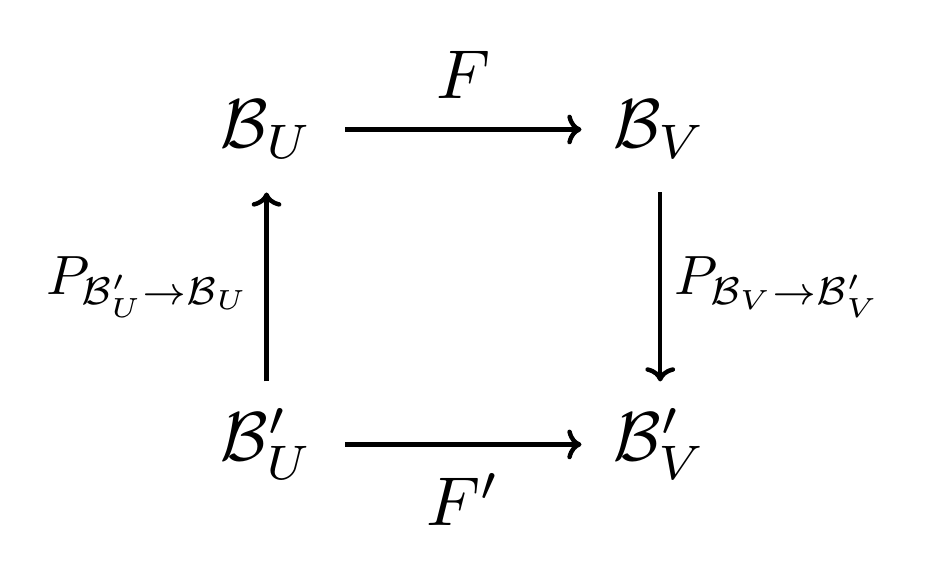
\begin{tikzpicture}
	\coordinate (U)  at (-2.5,+2);
	\coordinate (Ud) at (-2.5,-2);
	\coordinate (V)  at (+2.5,+2);
	\coordinate (Vd) at (+2.5,-2);
	
	\coordinate (F)  at (+0,+2.7);
	\coordinate (Fd) at (+0,-2.7);
	\coordinate (P1) at (-4,+0);
	\coordinate (P2) at (+4,+0);
	
	\node[black,scale=2.5] at (U)  {$\mathcal{B}_U$};
	\node[black,scale=2.5] at (Ud) {$\mathcal{B}'_U$};
	\node[black,scale=2.5] at (V)  {$\mathcal{B}_V$};
	\node[black,scale=2.5] at (Vd) {$\mathcal{B}'_V$};
	
	\node[black,scale=2.5] at (F)  {$F$};
	\node[black,scale=2.5] at (Fd) {$F'$};
	\node[black,scale=2] at (P1) {$P_{\mathcal{B}'_U\to\mathcal{B}_U}$};
	\node[black,scale=2] at (P2) {$P_{\mathcal{B}_V\to\mathcal{B}_V'}$};
	
	\draw[->,ultra thick] ($(U)+(1,0)$)--($(V)-(1,0)$);
	\draw[->,ultra thick] ($(Ud)+(1,0)$)--($(Vd)-(1,0)$);
	\draw[->,ultra thick] ($(Ud)+(0,0.8)$)--($(U)-(0,0.8)$);
	\draw[->,ultra thick] ($(V)-(0,0.8)$)--($(Vd)+(0,0.8)$);
\end{tikzpicture}
\end{figure}
To read this schematic, consider that the arrow for $F'$ has the same input and output as following the other three arrows to go up, then right (through $F$) then down again. This ordered path is the matrix multiplication given above.
}

\example{Changing the bases of a matrix representation}{

\noindent Consider the linear map $f:\mathbb{R}^2 \to \mathcal{P}_2$ given by
\begin{align*}
f(\alpha,\beta) = \beta + \alpha x^2.
\end{align*}
What is the matrix representation of $f$ using the canonical bases of $\mathbb{R}^2$, call it $\mathcal{A}$, and $\mathcal{P}_2$, call it $\mathcal{B}$? Consider the two bases $\mathcal{A}'=\{(-1,1),\, (1,2)\}$ and $\mathcal{B}'=\{ 2, \,1- x, \, 3 + x^2 \}$. Use transition matrices to find the matrix representation of $f$ in these new bases: $\mathcal{M}(f,\mathcal{A}'\to\mathcal{B}')$. \\

\noindent For the matrix in the canonical bases, we use the linear map on the basis vectors:
\begin{align*}
f(1,0) &= x^2 \implies [f(1,0)]_{\mathcal{B}} = \begin{pmatrix} 0 \\ 0 \\ 1\end{pmatrix} \\
f(0,1) &= 1 \implies [f(0,1)]_{\mathcal{B}} = \begin{pmatrix} 1 \\ 0 \\ 0\end{pmatrix}
\end{align*}
and so that matrix of $f$ in the canonical bases is given by
\begin{align*}
\mathcal{M}(f,\mathcal{A}\to\mathcal{B})
=
\begin{pmatrix} 
0 & 1 \\
0 & 0 \\
1 & 0
\end{pmatrix}
\end{align*}
We need transition matrices $P_{\mathcal{A}'\to\mathcal{A}}$ and $P_{\mathcal{B}\to\mathcal{B}'}$. The first is really simple
\begin{align*}
(-1,1) &= -1(1,0) + 1(0,1) \implies[(1,1)]_{\mathcal{A}} = \begin{pmatrix} -1 \\ 1 \end{pmatrix} \\
(1,2) &= 1(1,0) + 2(0,1) \implies[(0,2)]_{\mathcal{A}} = \begin{pmatrix} 1 \\ 2 \end{pmatrix} \\
\implies P_{\mathcal{A}'\to\mathcal{A}}
&=
\begin{pmatrix} 
 -1 & 1\\ 
  1 & 2
\end{pmatrix}
\end{align*}
The second transition matrix, from $\mathcal{B}=\{1,\,x,\,x^2\}$ to $\mathcal{B}'=\{2,\,1-x,\,3+x^2\}$, requires a bit more effort
\begin{align*}
1 &= \alpha(2) + \beta(1-x) + \gamma(3+x^2) \\
\implies &
\begin{cases}
2\alpha + \beta + 3\gamma = 1 \\
-\beta = 0 \\
\gamma = 0
\end{cases} \\
\implies & \alpha = 1/2 \\
\implies & [1]_{\mathcal{B}'} = \begin{pmatrix} 1/2 \\ 0 \\ 0 \end{pmatrix} \\ \\
%%
%%
x &= \alpha(2) + \beta(1-x) + \gamma(3+x^2) \\
\implies &
\begin{cases}
2\alpha + \beta + 3\gamma = 0 \\
-\beta = 1 \\
\gamma = 0
\end{cases} \\
\implies & \alpha = 0 \\
\implies & [x]_{\mathcal{B}'} = \begin{pmatrix} 0 \\ -1 \\ 0 \end{pmatrix} \\ \\
%%
%%
x^2 &= \alpha(2) + \beta(1-x) + \gamma(3+x^2) \\
\implies &
\begin{cases}
2\alpha + \beta + 3\gamma = 0 \\
-\beta = 0 \\
\gamma = 1
\end{cases} \\
\implies & \alpha = -3/2 \\
\implies & [x^2]_{\mathcal{B}'} = \begin{pmatrix} -3/2 \\ 0 \\ 1 \end{pmatrix}
\end{align*}
so we have transition matrix
\begin{align*}
P_{\mathcal{B}\to\mathcal{B}'}
&=
\begin{pmatrix} 
  1/2 & 0 & -3/2 \\
  0 & -1 & 0 \\
  0 & 0 & 1
\end{pmatrix}
\end{align*}
Now we can use these transition matrices to compute the matrix representation of $f$ in these alternate bases:
\begin{align*}
F' &= P_{\mathcal{B}\to\mathcal{B}'} \, F \, P_{\mathcal{A}'\to\mathcal{A}} \\
%%%
%%%
%%%
&= \begin{pmatrix} 
  1/2 & 0 & -3/2 \\
  0 & -1 & 0 \\
  0 & 0 & 1
\end{pmatrix}
\begin{pmatrix} 
  0 & 1 \\
  0 & 0 \\
  1 & 0
\end{pmatrix}
\begin{pmatrix} 
 -1 & 1 \\ 
  1 & 2
\end{pmatrix} \\
%%%
%%%
%%%
&=
\begin{pmatrix} 
  2 & -1/2 \\
  0 & 0 \\
 -1 & 1
\end{pmatrix}
\end{align*}
}
%\chapter{Eigenvalues and Eigenvectors} \label{ch:eigens}



\section{Basic definitions}

\definition{Eigenvalues and eigenvectors of a linear map}{
Consider an endomorphism $f:V \to V$ and a vector $\mathbf{v}\in V$. We call a number $\lambda$ an eigenvalue of $f$ if there exists a non-zero vector $\mathbf{v}$ satisfying the relation
\begin{align*}
f(\mathbf{v}) = \lambda \mathbf{v}.
\end{align*}
We say that $\mathbf{v}$ is an eigenvector of $f$ \textit{corresponding} or \textit{associated} to the eigenvalue $\lambda$.
}

\example{Eigenvalue of a linear map}{

\noindent Consider an endomporphism $f:\mathbb{R}^2 \to \mathbb{R}^2$ defined by
\begin{align*}
f(x,y) = (y,x)
\end{align*}
Can you find any eigenvalues and corresponding eigenvectors?

\noindent As this map just switches coordinates around, it's pretty clear that any input vector with equal $x$ and $y$ components will remain unchanged. That is, for example,
\begin{align*}
f(3,3) = (3,3)
\end{align*}
and hence $\lambda=1$ is an eigenvalue with corresponding eigenvector $(3,3)$. In fact every vector of the form $(k,k)$ corresponds to this eigenvalue, showing you that eigenvectors are not unique.
}

We will develop a technique for systematically finding eigenvalues and eigenvectors that works on the matrix representation of an endomorphism. As such, it will be typical that we instead refer to eigenvalues and eigenvectors \textit{of a matrix}, forgetting that there is an associated endomorphism behind the scenes. To reduce notational baggage, we will also stop referring explicitly to the coordinates of a vector in some basis, i.e. $[\mathbf{v}]_\mathcal{B}$, and instead just talk about a vector \textit{as though it is its coordinates}: $[\mathbf{v}]_\mathcal{B} \to \mathbf{v}$. So let's give this alternative definition which is equivalent.

\definition{Eigenvectors and eigenvalues of a matrix}{
For a square matrix $A$, an eigenvector of $A$ is a non-zero vector, $\mathbf{v}$, that satisfies the matrix equation
\begin{align*}
A\mathbf{v} = \lambda \mathbf{v}
\end{align*}
where $\lambda$ is called an eigenvalue of $A$. We say that $\mathbf{v}$ is an eigenvector of $A$ \textit{corresponding} or \textit{associated} to the eigenvalue $\lambda$.
}

\example{Eigenvalue of a matrix}{

\noindent Consider the matrix
\begin{align*}
A
=
\begin{pmatrix}
0 & 1 \\
1 & 0
\end{pmatrix}
\end{align*}
which is the matrix of the endomorphism of the previous example in the canonical bases. Show that the vector
\begin{align*}
\mathbf{v}= 
\begin{pmatrix}
2\\
2
\end{pmatrix}
\end{align*}
is an eigenvector and find the associated eigenvalue. \\

\noindent Hit the vector with the matrix and look at the result:
\begin{align*}
A\mathbf{v} &= 
\begin{pmatrix}
0 & 1 \\
1 & 0
\end{pmatrix}
\begin{pmatrix}
2\\
2
\end{pmatrix} \\
&= 
\begin{pmatrix}
2\\
2
\end{pmatrix} \\
&= 1 \mathbf{v}
\end{align*}
This shows that $A\mathbf{v} = 1\mathbf{v}$, so that $\mathbf{v}$ is an eigenvector, associated to the same eigenvalue $\lambda=1$ as we found in the previous example.
}

What is really going on here with these eigenvectors? Well, if you think geometrically, the multiplication $A\mathbf{v}$ represents a transformation of an arrow in $\mathbb{R}^n$ to give another arrow in $\mathbb{R}^n$ (because $A$ represents an endomorphism the input and output spaces are the same). An eigenvector is a special direction that just so happens to transform under $A$ merely by scaling. The equation $A\mathbf{v} = \lambda\mathbf{v}$ means the action of $A$ on the eigenvector is to maintain it in the same direction, but to change its length only. Ok, now lets start to develop the systematic search for eigenvalues.

We start with a rearrangement of the fundamental equation
\begin{align*}
A\mathbf{v} = \lambda\mathbf{v} \implies A\mathbf{v} - \lambda\mathbf{v} = \mathbf{0}.
\end{align*}
Now it looks like $\mathbf{v}$ is a common factor that can be factorised. But we must be careful not to write nonsense: $A-\lambda$ would be a matrix subtracted by a real number. Thankfully this isn't a problem:
\begin{align*}
A\mathbf{v} - \lambda\mathbf{v} = \mathbf{0} \\
A\mathbf{v} - \lambda I\mathbf{v} = \mathbf{0} \\
\left(A - \lambda I\right)\mathbf{v} = \mathbf{0}
\end{align*}
where $I$ is the identity matrix of the same size as $A$. This means that $A - \lambda I$ is a matrix, where $\lambda I$ is a matrix with only $\lambda$ along the diagonal and zeros everywhere else. Let's consider this matrix closely, first by naming its determinant.

\definition{Characteristic polynomial of a matrix}{
For a square matrix $A$, the \textit{characteristic polynomial} is the given by
\begin{align*}
P(\lambda) = \det ( A - \lambda I)
\end{align*}
where $I$ is the identity matrix with the same size as $A$ and $\lambda$ is the variable of the polynomial. The degree of this polynomial is always the same as the size of the matrix $A$.
}

\noindent Why is this polynomial important? Well we want the equation
\begin{align*}
\left(A - \lambda I\right)\mathbf{v} = \mathbf{0}
\end{align*}
to be true, while also requiring that the vector $\mathbf{v}$ be non-zero. Now if $A - \lambda I$ was an invertible matrix, we could simply multiply both sides by its inverse and determine that $\mathbf{v}=\mathbf{0}$. This means we require that $A - \lambda I$ be non-invertible, which implies that its determinant is zero. So we can require that eigenvalues are such that the characteristic polynomial is zero. That is the beginning of our systematic technique, defined below.

\definition{Eigenspectrum}{
The eigenvalues of a square matrix $A$ are roots of the characteristic polynomial of $A$. That is, eigenvalues are solutions of
\begin{align*}
 \det ( A - \lambda I) = 0.
\end{align*} 
There can be multiple distinct eigenvalues of $A$, and are conventionally denoted $\lambda_1$, $\lambda_2$, \dots etc. The set of these eigenvalues, $\{\lambda_1, \, \lambda_2, \dots \}$, is called the \textit{eigenspectrum} of $A$.
}

\example{Eigenspectrum of a 3 by 3 matrix}{

\noindent Consider the matrix
\begin{align*}
A
=
\begin{pmatrix}
 -2 &  2 &  3 \\
  1 &  0 & -1 \\
  0 &  3 &  1
\end{pmatrix}
\end{align*}
Give its characteristic polynomial and hence determine the eigenvalues. \\

\noindent The characteristic polynomial is the determinant
\begin{align*}
P(\lambda) &= |A - \lambda I| 
= \left| 
\begin{pmatrix}
 -2 &  2 &  3 \\
  1 &  0 & -1 \\
  0 &  3 &  1
\end{pmatrix}
-
\begin{pmatrix}
 \lambda &  0 &  0 \\
  0 &  \lambda & 0 \\
  0 &  0 & \lambda
\end{pmatrix}
\right|
= \left| 
\begin{matrix}
 -2-\lambda &  2 &  3 \\
  1 &  -\lambda & -1 \\
  0 &  3 &  1-\lambda
\end{matrix}
\right| \\
%%
%%
%%
&= 
(-2-\lambda) \left| 
\begin{matrix}
    -\lambda & -1 \\
    3 &  1-\lambda
\end{matrix}
\right|
-
1 \left| 
\begin{matrix}
    2 & 3 \\
    3 &  1-\lambda
\end{matrix}
\right| \\
%%
%%
%%
&= 
(-2-\lambda) \left( \lambda^2 + 3\right) - \left(2-2\lambda - 9\right) \\
&= -\lambda^3 - \lambda^2 + \lambda + 1
\end{align*}
By inspection we have $P(1)=0$, and so $\lambda-1$ is a factor of $P(\lambda)$. With long division we find the other factor is $-\lambda^2 - 2 \lambda - 1 = -(\lambda + 1)^2$ and so the characteristic polynomial is
\begin{align*}
P(\lambda) = (1-\lambda)(1+\lambda)^2
\end{align*}
The roots of $P(\lambda)$ give the eigenspectrum: $\{1, -1\}$.
}

\theorem{Number of eigenvalues up to the size of the matrix}{
A square matrix of size $n$ has up to $n$ distinct eigenvalues.
}


\noindent Consider the matrix
\begin{align*}
A = 
\begin{pmatrix}
  1 & -2 & -2 \\
 -2 &  1 & -1 \\
 -1 & -1 &  2
\end{pmatrix}.
\end{align*}
You should verify, but consider the following multiplications
\begin{align*}
A \begin{pmatrix} -1 \\ 1 \\ 0 \end{pmatrix} = 3 \begin{pmatrix} -1 \\ 1 \\ 0 \end{pmatrix} \quad \text{and} \quad
A \begin{pmatrix} -1 \\ 0 \\ 1 \end{pmatrix} = 3 \begin{pmatrix} -1 \\ 0 \\ 1 \end{pmatrix}.
\end{align*}
This shows that there can be multiple eigenvectors associated to the same eigenvalue. In fact there are always infinite vectors, because we can use the linearity of matrix multiplication to show, for example,
\begin{align*}
A \left( \alpha \begin{pmatrix} -1 \\ 1 \\ 0 \end{pmatrix} +
\beta \begin{pmatrix} -1 \\ 0 \\ 1 \end{pmatrix} \right) &= \left( \alpha A\begin{pmatrix} -1 \\ 1 \\ 0 \end{pmatrix} +
\beta A\begin{pmatrix} -1 \\ 0 \\ 1 \end{pmatrix} \right) \\ 
&= \left( \alpha 3\begin{pmatrix} -1 \\ 1 \\ 0 \end{pmatrix} +
\beta 3\begin{pmatrix} -1 \\ 0 \\ 1 \end{pmatrix} \right) \\
&= 3\left( \alpha \begin{pmatrix} -1 \\ 1 \\ 0 \end{pmatrix} +
\beta \begin{pmatrix} -1 \\ 0 \\ 1 \end{pmatrix} \right)
\end{align*}
meaning that any linear combination of eigenvectors is also an eigenvector. That inspires us to consider instead a \textit{space of eigenvectors} associated to an eigenvalue.

\definition{Eigenspace}{
For any eigenvalue $\lambda_k$ of an $n \times n$ matrix $A$, the eigenspace corresponding to $\lambda_k$, denoted $E_{\lambda_k}$, is the set of all eigenvectors corresponding to $\lambda_k$. This can be written as the set of linear combinations of linearly independent eigenvectors corresponding to $\lambda_k$:
\begin{gather*}
E_{\lambda_k} = \{ \alpha_1 \mathbf{v}_1 + \cdots + \alpha_m \mathbf{v}_m \, | \, \forall j \, A \mathbf{v}_j = \lambda_k \mathbf{v}_j, \, \alpha_j \in \mathbb{R} \} = \text{SPAN}(\mathbf{v}_1, \cdots, \mathbf{v}_m) \\
\text{for maximum number of eigenvectors such that} \\
\alpha_1 \mathbf{v}_1 + \cdots + \alpha_m \mathbf{v}_m = \mathbf{0} \implies  \alpha_1 =  \alpha_2 = \cdots = \alpha_m = 0.
\end{gather*}
As the set $\{\mathbf{v}_1, \cdots, \mathbf{v}_m\}$ generates $E_{\lambda_k}$ and the vectors are linearly independent, the set forms a basis and therefore gives the dimension $E_{\lambda_k}$.

The eigenspace can also be written like a \textit{kernel}
\begin{align*}
E_{\lambda_k} = \{ \mathbf{v} \in \mathbb{R}^n \, | \, \left( A - \lambda_k I \right) \mathbf{v}= \mathbf{0} \}.
\end{align*}
}

\example{Eigenspace}{
\label{ex:espaces-degen}

\noindent Take the matrix of the previous example
\begin{align*}
A
=
\begin{pmatrix}
 -2 &  2 &  3 \\
  1 &  0 & -1 \\
  0 &  3 &  1
\end{pmatrix}
\end{align*}
Determine the eigenspaces of all eigenvalues of $A$. \\

\noindent We showed that $\lambda_1=1$ and $\lambda_2=-1$ are two eigenvalues of $A$. So we are looking for two vector spaces
\begin{align*}
E_{\lambda_1} = \{ \mathbf{v} \in \mathbb{R}^3 \, | \, \left( A -  I \right) \mathbf{v}=0 \} \quad \text{and} \quad E_{\lambda_2} = \{ \mathbf{v} \in \mathbb{R}^3 \, | \, \left( A +  I \right) \mathbf{v}= \mathbf{0} \}
\end{align*}
For $\lambda_1$ we are therefore looking for all the triples that satisfy $\left( A -  I \right) \mathbf{v}$. Let the undetermined eigenvector be written
\begin{align*}
\mathbf{v} = \begin{pmatrix} x \\ y \\ z \end{pmatrix}.
\end{align*}
Our goal is to find all possible $x$, $y$ and $z$ such that
\begin{align*}
& \left( A -  I \right) \mathbf{v}= \mathbf{0} \\
%%
%%
%%
\implies &
\left(
\begin{pmatrix}
 -2 &  2 &  3 \\
  1 &  0 & -1 \\
  0 &  3 &  1
\end{pmatrix}
-
\begin{pmatrix}
  1 &  0 &  0 \\
  0 &  1 &  0 \\
  0 &  0 &  1
\end{pmatrix}
\right) 
\begin{pmatrix} x \\ y \\ z \end{pmatrix}
= 
\begin{pmatrix}
  0 \\
  0  \\
  0 
\end{pmatrix}
\\
%%
%%
%%
\implies &
\begin{pmatrix}
 -3 &  2 &  3 \\
  1 & -1 & -1 \\
  0 &  3 &  0
\end{pmatrix}
\begin{pmatrix} x \\ y \\ z \end{pmatrix}
= 
\begin{pmatrix}
  0 \\
  0 \\
  0 
\end{pmatrix}
\end{align*}
This is a regular matrix equation that we solve with the techniques of linear systems (see appendix...). So we perform Gaussian reduction on an augmented matrix
\begin{align*}
\left(
	\begin{matrix}
 -3 &  2 &  3 \\
  1 & -1 & -1 \\
  0 &  3 &  0
	\end{matrix}
  \left| \, 
	\begin{matrix}
  0 \\
  0 \\
  0 
	\end{matrix}
  \right.
\right)
\to
\left(
	\begin{matrix}
  1 &  0 & -1 \\
  0 &  1 &  0 \\
  0 &  0 &  0
	\end{matrix}
  \left| \, 
	\begin{matrix}
	  0 \\
	  0 \\
	  0 
    \end{matrix}
  \right.
\right)
\end{align*}
Unpacking this last matrix gives the equations
\begin{align*}
& x - z = 0 \\
& y=0
\end{align*}
And so any eigenvector associated with $\lambda_1=1$ must have the form
\begin{align*}
\mathbf{v} = \begin{pmatrix} z \\ 0 \\ z \end{pmatrix}
= z\begin{pmatrix} 1 \\ 0 \\ 1 \end{pmatrix}.
\end{align*}
As $z$ is a free variable, this says all multiples of $(1,\,0,\,1)$ will satisfy $(A-I)\mathbf{v}=\mathbf{0}$. So we can write the eigenspace associated with this eigenvalue
\begin{align*}
E_{\lambda_1} = \{ k(1,\,0,\,1) \, | \, k \in \mathbb{R} \} = \text{SPAN} \left((1,\,0,\,1)\right).
\end{align*}

For $\lambda_2=-1$ we look for all the triples that satisfy $\left( A +  I \right) \mathbf{v}$. Let the undetermined eigenvector be written
\begin{align*}
\mathbf{v} = \begin{pmatrix} x \\ y \\ z \end{pmatrix}.
\end{align*}
The eigenvector therefore equation gives
\begin{align*}
& \begin{pmatrix}
 -1 &  2 &  3 \\
  1 &  1 & -1 \\
  0 &  3 &  2
\end{pmatrix}
\begin{pmatrix} x \\ y \\ z \end{pmatrix}
= 
\begin{pmatrix}
  0 \\
  0  \\
  0 
\end{pmatrix}
\\
%%
%%
%%
\implies &
\left(
	\begin{matrix}
 -1 &  2 &  3 \\
  1 &  1 & -1 \\
  0 &  3 &  2
	\end{matrix}
  \left| \, 
	\begin{matrix}
  0 \\
  0 \\
  0 
	\end{matrix}
  \right.
\right)
\to
\left(
	\begin{matrix}
  1 &  0 & -5/3 \\
  0 &  1 &  2/3 \\
  0 &  0 &  0
	\end{matrix}
  \left| \, 
	\begin{matrix}
	  0 \\
	  0 \\
	  0 
    \end{matrix}
  \right.
\right)
\end{align*}
Unpacking this last matrix gives the equations
\begin{align*}
& x - (5/3)z = 0 \\
& y + (2/3)z = 0
\end{align*}
And so any eigenvector associated with $\lambda_1=1$ must have the form
\begin{align*}
\mathbf{v} = \begin{pmatrix} (5/3)z \\ -(2/3)z \\ z \end{pmatrix}
= \frac{z}{3}\begin{pmatrix} 5 \\ -2 \\ 3 \end{pmatrix}.
\end{align*}
As $z$ is arbitrary, $z/3$ is also arbitrary. Note that I took this out of the triple as $z/3$ only to force a triple of integers. It's not necessary and I could have written $(5/3, \, 2/3, \, 1)$. So all multiples of $(5,\,2,\,3)$ will satisfy $(A+I)\mathbf{v}=\mathbf{0}$ and we can write the eigenspace associated with this eigenvalue
\begin{align*}
E_{\lambda_2} = \{ k(5,\,-2,\,3) \, | \, k \in \mathbb{R} \} = \text{SPAN} \left((5,\,-2,\,3)\right).
\end{align*}
We can verify, for example, that the vector $(15,-6,9)$ is an eigenvector with eigenvalue $-1$ with a quick multiplication
\begin{align*}
\begin{pmatrix}
 -2 &  2 &  3 \\
  1 &  0 & -1 \\
  0 &  3 &  1
\end{pmatrix}
\begin{pmatrix}
 15 \\ -6 \\ 9
\end{pmatrix}
=
\begin{pmatrix}
 -30 - 12 + 27 \\ 15 - 9 \\ -18 + 9
\end{pmatrix}
=
\begin{pmatrix}
 -15 \\ 6 \\ -9
\end{pmatrix}
=
-1
\begin{pmatrix}
 15 \\ -6 \\ 9
\end{pmatrix}
\end{align*}
}

\definition{Algebraic and geometric multiplicity of an eigenvalue}{
For an $n \times n$ matrix with characteristic polynomial
\begin{align*}
P(\lambda) = C(\lambda - \lambda_1)^{m_1} \times \cdot \times (\lambda - \lambda_k)^{m_k}\times  \cdot \times (\lambda - \lambda_p)^{m_p}
\end{align*}
for some constant $C$, there can be up to $n$ distinct eigenvalues ($p \leq n$). The exponent $m_k$ is called the \textcolor{airforceblue}{\textit{algebraic} multiplicity} of the eigenvalue $\lambda_k$. The \textit{dimension} of the eigenspace corresponding to $\lambda_k$ is its \textcolor{brightmaroon}{\textit{geometric} multiplicity}.
}


\noindent For the matrix of the previous example
\begin{align*}
A
=
\begin{pmatrix}
 -2 &  2 &  3 \\
  1 &  0 & -1 \\
  0 &  3 &  1
\end{pmatrix}
\end{align*}
we found that the characteristic polynomial was $P(\lambda) = -(\lambda - 1)(\lambda - (-1))^2$ giving the eigenspectrum $\{\lambda_1, \lambda_2\}=\{1, -1\}$ and eigenspaces
\begin{align*}
E_{\lambda_1} = \{ k(1,\,0,\,1) \, | \, k \in \mathbb{R} \} \quad \text{and} \quad E_{\lambda_2} = \{ k(5,\,-2,\,3) \, | \, k \in \mathbb{R} \}.
\end{align*}
This means that the geometric multiplicity of both eigenvalues is 1, while the algebraic multiplicity of $\lambda_2$ is 2. The lesson here is that the two types of multiplicity are not necessarily equal. Let's take another example.

\example{Eigenvalue multiplicity}{

\noindent Consider the matrix
\begin{align*}
A =
\begin{pmatrix}
  1 & -1 &  0 \\
  0 &  2 &  0 \\
 -1 & -1 &  2
\end{pmatrix}
\end{align*}
The characteristic polynomial is $P(\lambda)=-(\lambda-1)(\lambda-2)^2$. Determine the eigenspaces of $A$ and therefore the geometric multiplicities of its eigenvalues. \\

\noindent For eigenvalue $\lambda_1=1$, of algebraic multiplicity 1, we search for triples $(x,y,z)$ such that
\begin{align*}
&
\left(\begin{pmatrix}
  1 & -1 &  0 \\
  0 &  2 &  0 \\
 -1 & -1 &  2
\end{pmatrix}
-
1
\begin{pmatrix}
  1 &  0 &  0 \\
  0 &  1 &  0 \\
  0 &  0 &  1
\end{pmatrix}\right)
\begin{pmatrix}
  x \\
  y \\
  z
\end{pmatrix}
=
\begin{pmatrix}
  0 \\
  0 \\
  0
\end{pmatrix} \\
%%
%%
%%
\implies &
\left(
	\begin{matrix}
  0 & -1 &  0 \\
  0 &  1 &  0 \\
 -1 & -1 &  1
	\end{matrix}
  \left| \, 
	\begin{matrix}
  0 \\
  0 \\
  0 
	\end{matrix}
  \right.
\right)
\to
\left(
	\begin{matrix}
 -1 &  0 &  1 \\
  0 &  1 &  0 \\
  0 &  0 &  0 \\
	\end{matrix}
  \left| \, 
	\begin{matrix}
	  0 \\
	  0 \\
	  0 
    \end{matrix}
  \right.
\right)
\end{align*}
So we have $y=0$ and $x=z$. The eigenspace is therefore
\begin{align*}
E_{\lambda_1} = \{ k(1,0,1) \, | \, k\in\mathbb{R} \, \} = \text{SPAN}((1,0,1))
\end{align*}
As this is a 1 dimensional space, $\lambda_1$ has geometric multiplicity 1.

For eigenvalue $\lambda_1=2$, of algebraic multiplicity 2, we search for triples $(x,y,z)$ such that
\begin{align*}
&
\left(\begin{pmatrix}
  1 & -1 &  0 \\
  0 &  2 &  0 \\
 -1 & -1 &  2
\end{pmatrix}
-
2
\begin{pmatrix}
  1 &  0 &  0 \\
  0 &  1 &  0 \\
  0 &  0 &  1
\end{pmatrix}\right)
\begin{pmatrix}
  x \\
  y \\
  z
\end{pmatrix}
=
\begin{pmatrix}
  0 \\
  0 \\
  0
\end{pmatrix} \\
%%
%%
%%
\implies &
\left(
	\begin{matrix}
 -1 & -1 &  0 \\
  0 &  0 &  0 \\
 -1 & -1 &  0
	\end{matrix}
  \left| \, 
	\begin{matrix}
  0 \\
  0 \\
  0 
	\end{matrix}
  \right.
\right)
\to
\left(
	\begin{matrix}
  1 &  1 &  0 \\
  0 &  0 &  0 \\
  0 &  0 &  0 \\
	\end{matrix}
  \left| \, 
	\begin{matrix}
	  0 \\
	  0 \\
	  0 
    \end{matrix}
  \right.
\right)
\end{align*}
So we have free variables $z$ and $y$, with $x=-y$. The triple can therefore be written
\begin{align*}
(x,y,z) = (-y,y,z) = y(-1,1,0) + z(0,0,1).
\end{align*}
The eigenspace is therefore
\begin{align*}
E_{\lambda_2} = \{ (x,y,z)\in\mathbb{R}^2 \, | \, x=-y \} = \text{SPAN}((-1,1,0), \, (0,0,1)).
\end{align*}
As this is a 2 dimensional space, $\lambda_2$ has geometric multiplicity 2.
}

\theorem{Linear independence of eigenvectors}{
Eigenvectors from different eigenspaces are linearly independent.
}


\definition{Eigenbasis}{
Consider a square matrix $A$ of size $n$. If the dimensions of its eigenspaces add up to $n$, then there exist $n$ linearly independent eigenvectors of $A$. These eigenvectors form a basis of $\mathbb{R}^n$ called an \textit{eigenbasis}.
}

\noindent In the previous example, for matrix
\begin{align*}
A =
\begin{pmatrix}
  1 & -1 &  0 \\
  0 &  2 &  0 \\
 -1 & -1 &  2
\end{pmatrix}
\end{align*}
we found eigenspaces 
\begin{align*}
E_{\lambda_1} = \text{SPAN}((1,0,1)) \quad \text{and} \quad
E_{\lambda_2} = \text{SPAN}((-1,1,0), \, (0,0,1)).
\end{align*}
with dimensions adding up to the same size as the matrix. So we can form an eigenbasis of $\mathbb{R}^3$ out of eigenvectors:
\begin{align*}
\mathcal{E} = \{ (1,0,1), \, (-1,1,0), \, (0,0,1) \}.
\end{align*}
Note that this eigenbasis is \textit{not unique}. $E_{\lambda_2}$ is a plane, and so any 2 independent vectors in this plane will work. So for example we can write another eigenbasis
\begin{align*}
\mathcal{E}' = \{ (3,0,3), \, (2,-2,1), \, (0,0,-3) \}.
\end{align*}

\section{Eigenvalue diagonalization}


In the previous chapter we saw that the matrix representation of linear map, $f:U\to V$, depends on the chosen bases. In Theorem~\ref{thm:map_diff_bases} we showed how to relate different matrix representations of the same map by using transition matrices:
\begin{align*}
\mathcal{M}(f,\mathcal{A}',\mathcal{B}') = P_{\mathcal{B}\to\mathcal{B}'} \, \mathcal{M}(f,\mathcal{A},\mathcal{B}) \, P_{\mathcal{A}'\to\mathcal{A}}
\end{align*}
where $\mathcal{A}$ and $\mathcal{A}'$ are bases of $U$ and $\mathcal{B}$ and $\mathcal{B}'$ are bases of $V$. For an endomorphism the input and output vector spaces are the same, and so we only have two bases to consider, for example $\mathcal{A}$ and $\mathcal{A}'$:
\begin{align*}
\mathcal{M}(f,\mathcal{A}') = P_{\mathcal{A}\to\mathcal{A}'} \, \mathcal{M}(f,\mathcal{A}) \, P_{\mathcal{A}'\to\mathcal{A}}
\end{align*}
We also saw that the inverse of a transition matrices is simply a transition matrix in the reverse direction of bases. So we can in fact write
\begin{align*}
\mathcal{M}(f,\mathcal{A}') = P \, \mathcal{M}(f,\mathcal{A}) \, P^{-1}
\end{align*}
where $P=P_{\mathcal{A}\to\mathcal{A}'}$. As stated previously, we are going to abstract away from linear maps, and just consider all these results acting on matrices only, and pretty much forget that there is some associated linear map underneath it all. So we abstract away this form by introducing the following definition.

\definition{Similar matrices}{
Two matrices $A$ and $B$ are similar if there exists an invertible matrix $P$ such that
\begin{align*}
B = P A P^{-1}.
\end{align*}
}

Why is this property interesting? Well for one thing it possibly simplifies the calculation of powers of a matrix. If $A$ and $B$ are similar matrices, then
\begin{align*}
B^n &= (P A P^{-1})^n = (P A P^{-1})\times (P A P^{-1})\times  \cdots \times (P A P^{-1})(P A P^{-1}) \\
&=  P A (P^{-1}P) A (P^{-1}\times  \cdots \times P) A( P^{-1} P) A P^{-1} \\
&=  P A A \times  \cdots \times P) A A P^{-1} \\
&=  P A^n P^{-1}.
\end{align*}
What this shows is that we can transfer the difficulty of a calculation of powers of a matrix $B$ towards another matrix $A$, hoping that it might be easier. Of course we will find ways to find very nice $A$ matrices. Note that taking powers of diagonal matrices are particularly nice
\begin{align*}
\begin{pmatrix}
 a_{11} &   0    & \dots  &   0 \\
   0    & a_{22} & \dots  &   0 \\
 \vdots & \vdots & \ddots & \vdots \\
   0    &   0    & \cdots & a_{nn}
\end{pmatrix}^k
=
\begin{pmatrix}
 a_{11}^k &   0    & \dots  &   0 \\
   0    & a_{22}^k & \dots  &   0 \\
 \vdots & \vdots & \ddots & \vdots \\
   0    &   0    & \cdots & a_{nn}^k
\end{pmatrix}
\end{align*}
so it would be nice to find out that a given matrix is similar to a diagonal matrix, eh?


\definition{Diagonalizable linear map}{
Let $f:V\to V$ be an endomorphism. $f$ is called \textit{diagonalizable} if there exists a basis, $\mathcal{B}$, of $V$ such that the matrix representation of $f$ in $\mathcal{B}$ is diagonal:
\begin{align*}
(\mathcal{M}(f,\mathcal{B}))_{ij} = 0 \quad \text{whenever } \, i \neq j.
\end{align*}
}

\noindent As we've done again and again this chapter, we will instead transfer this property over to a matrix and forget about the linear map.


\definition{Diagonalizable matrix}{
A square matrix $A$ is \textit{diagonalizable} if and only if there exists an invertible matrix $P$ and diagonal matrix $D$ such that
\begin{align*}
A = P D P^{-1}.
\end{align*}
Alternative: A square matrix $A$ is \textit{diagonalizable} if and only if it is \textit{similar} to a diagonal matrix $D$. 
}

\noindent Now we bring eigenvalues into the picture, because they can sometimes give us a particularly simple technique for diagonalizing a matrix.


\theorem{Eigenvalue diagonalization}{
A square matrix $A$ of size $n$ is diagonalizable if and only if there exists an eigenbasis of $\mathbb{R}^n$. We can then define a diagonal matrix consisting of the eigenvalues of $A$, $\lambda_1, \, \dots, \, \lambda_m$ with $m \leq n$ along the diagonal. In this case we write
\begin{align*}
A = P D P^{-1}
\end{align*}
where $P$ consists of eigenvectors of $A$ as columns \textit{in the order that corresponds to their eigenvalue placement in $D$}. The matrix $P$ is the transition matrix from the eigenbasis, $\mathcal{E}$, to the canonical basis of $\mathbb{R}^n$: $P_{\mathcal{E}\to \mathcal{C}_n}$. The following diagram summarises the relations between these different matrices and bases
\begin{figure}[H]
\centering
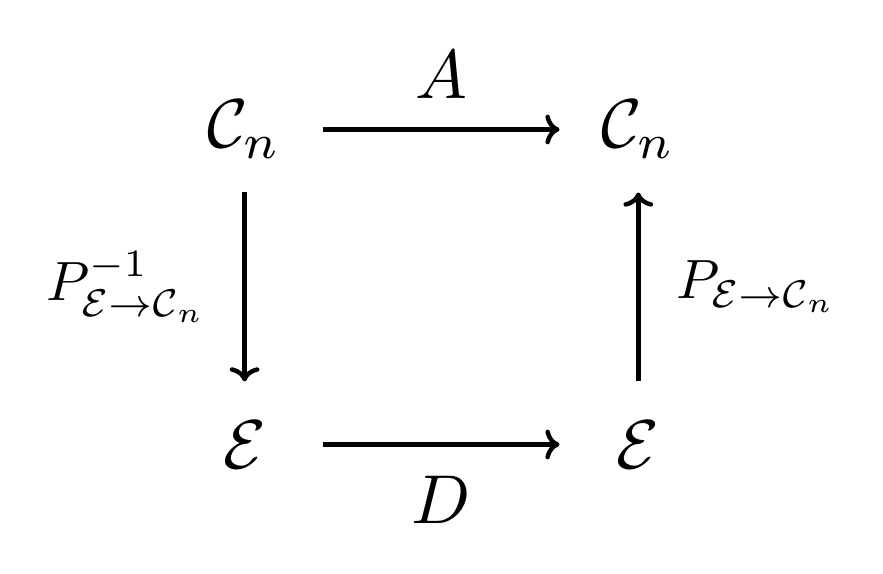
\begin{tikzpicture}
	\coordinate (Cn1)  at (-2.5,+2);
	\coordinate (E1) at (-2.5,-2);
	\coordinate (Cn2)  at (+2.5,+2);
	\coordinate (E2) at (+2.5,-2);
	
	\coordinate (F)  at (+0,+2.7);
	\coordinate (Fd) at (+0,-2.7);
	\coordinate (P1) at (-4,+0);
	\coordinate (P2) at (+4,+0);
	
	\node[black,scale=2.5] at (Cn1)  {$\mathcal{C}_n$};
	\node[black,scale=2.5] at (E1) {$\mathcal{E}$};
	\node[black,scale=2.5] at (Cn2)  {$\mathcal{C}_n$};
	\node[black,scale=2.5] at (E2) {$\mathcal{E}$};
	
	\node[black,scale=2.5] at (F)  {$A$};
	\node[black,scale=2.5] at (Fd) {$D$};
	\node[black,scale=2] at (P1) {$P_{\mathcal{E}\to\mathcal{C}_n}^{-1}$};
	\node[black,scale=2] at (P2) {$P_{\mathcal{E}\to\mathcal{C}_n}$};
	
	\draw[->,ultra thick] ($(Cn1)+(1,0)$)--($(Cn2)-(1,0)$);
	\draw[->,ultra thick] ($(E1)+(1,0)$)--($(E2)-(1,0)$);
	\draw[<-,ultra thick] ($(E1)+(0,0.8)$)--($(Cn1)-(0,0.8)$);
	\draw[<-,ultra thick] ($(Cn2)-(0,0.8)$)--($(E2)+(0,0.8)$);
\end{tikzpicture}
\end{figure}
}

\example{Eigenvalue diagonalization}{

\noindent Consider an endomorphism $f:\mathbb{R}^3 \to \mathbb{R}^3$ with matrix in the canonical bases given by
\begin{align*}
A = \mathcal{M}(f,\mathcal{C}_3) = 
\begin{pmatrix}
  1 & -3 & -1 \\
 -3 &  2 & -3 \\
  1 &  0 &  3
\end{pmatrix}.
\end{align*}
Diagonalize $A$ using its eigenvalues. \\

\noindent First we find the characteristic polynomial of $A$:
\begin{align*}
P(\lambda) &= |A - \lambda I| =
\left|
\begin{matrix}
  1-\lambda & -3 & -1 \\
 -3 &  2-\lambda & -3 \\
  1 &  0 &  3-\lambda
\end{matrix}
\right| =
1
\left|
\begin{matrix}
  -3 & -1 \\
   2-\lambda & -3 
\end{matrix}
\right|
+(3-\lambda)
\left|
\begin{matrix}
  1-\lambda & -3 \\
 -3 &  2-\lambda
\end{matrix}
\right| \\
%%
%%
%%
&= - \lambda^3 + 6\lambda^2 -3\lambda-10
\end{align*}
By inspection $P(-1)=0$ and so $(\lambda + 1)$ is a factor. With long division we find
\begin{align*}
P(\lambda) = (\lambda + 1)(-\lambda^2 + 7 \lambda - 10) = -(\lambda + 1)(\lambda-2)(\lambda-5).
\end{align*}
Hence the eigenspectrum is $\{\lambda_1, \, \lambda_2, \, \lambda_3 \} = \{-1,\,2,\,5\}$.

\noindent For $\lambda_1=-1$ we need to solve
\begin{align*}
& \begin{pmatrix}
  2 & -3 & -1 \\
 -3 &  3 & -3 \\
  1 &  0 &  4
\end{pmatrix}
\begin{pmatrix} x \\ y \\ z \end{pmatrix}
= 
\begin{pmatrix}
  0 \\
  0  \\
  0 
\end{pmatrix}
\\
%%
%%
%%
\implies &
\left(
	\begin{matrix}
  2 & -3 & -1 \\
 -3 &  3 & -3 \\
  1 &  0 &  4
	\end{matrix}
  \left| \, 
	\begin{matrix}
  0 \\
  0 \\
  0 
	\end{matrix}
  \right.
\right)
\to
\left(
	\begin{matrix}
  1 &  0 &  4 \\
  0 &  1 &  3 \\
  0 &  0 &  0
	\end{matrix}
  \left| \, 
	\begin{matrix}
	  0 \\
	  0 \\
	  0 
    \end{matrix}
  \right.
\right)
\end{align*}
Giving constraints $x=-4z$ and $y=-3z$ so that the eigenspace is given by
\begin{align*}
E_{\lambda_1} = \text{SPAN}((4,\,3,\,-1)).
\end{align*}

\noindent For $\lambda_2=2$ we need to solve
\begin{align*}
& \begin{pmatrix}
 -1 & -3 & -1 \\
 -3 &  0 & -3 \\
  1 &  0 &  1
\end{pmatrix}
\begin{pmatrix} x \\ y \\ z \end{pmatrix}
= 
\begin{pmatrix}
  0 \\
  0  \\
  0 
\end{pmatrix}
\\
%%
%%
%%
\implies &
\left(
	\begin{matrix}
 -1 & -3 & -1 \\
 -3 &  0 & -3 \\
  1 &  0 &  1
	\end{matrix}
  \left| \, 
	\begin{matrix}
  0 \\
  0 \\
  0 
	\end{matrix}
  \right.
\right)
\to
\left(
	\begin{matrix}
  1 &  0 &  1 \\
  0 & -3 &  0 \\
  0 &  0 &  0
	\end{matrix}
  \left| \, 
	\begin{matrix}
	  0 \\
	  0 \\
	  0 
    \end{matrix}
  \right.
\right)
\end{align*}
Giving constraints $x=-z$ and $y=0$ so that the eigenspace is given by
\begin{align*}
E_{\lambda_2} = \text{SPAN}((1,\,0,\,-1)).
\end{align*}

\noindent For $\lambda_3=5$ we need to solve
\begin{align*}
& \begin{pmatrix}
 -4 & -3 & -1 \\
 -3 & -3 & -3 \\
  1 &  0 & -2
\end{pmatrix}
\begin{pmatrix} x \\ y \\ z \end{pmatrix}
= 
\begin{pmatrix}
  0 \\
  0  \\
  0 
\end{pmatrix}
\\
%%
%%
%%
\implies &
\left(
	\begin{matrix}
 -4 & -3 & -1 \\
 -3 & -3 & -3 \\
  1 &  0 & -2
	\end{matrix}
  \left| \, 
	\begin{matrix}
  0 \\
  0 \\
  0 
	\end{matrix}
  \right.
\right)
\to
\left(
	\begin{matrix}
  1 &  0 & -2 \\
  0 &  1 &  3 \\
  0 &  0 &  0
	\end{matrix}
  \left| \, 
	\begin{matrix}
	  0 \\
	  0 \\
	  0 
    \end{matrix}
  \right.
\right)
\end{align*}
Giving constraints $x=2z$ and $y=-3z$ so that the eigenspace is given by
\begin{align*}
E_{\lambda_2} = \text{SPAN}((2,\,-3,\,1)).
\end{align*}
So we can write the diagonal matrix $D$ using the eigenvalues
\begin{align*}
D = 
 \begin{pmatrix}
 -1 &  0 &  0 \\
  0 &  2 &  0 \\
  0 &  0 &  5
 \end{pmatrix}
\end{align*}
and the matrix $P$ with eigenvectors as columns \textit{in an order so that the eigenvector columns correspond to the eigenvalue order in $D$}:
\begin{align*}
P = 
 \begin{pmatrix}
  4 &  1 &  2 \\
  3 &  0 & -3 \\
 -1 & -1 &  1
 \end{pmatrix}
\end{align*}
Recall, this is the transition matrix from the eigenbasis, $\mathcal{E} = \{(4,\,3,\,-1),\, (1,\,0,\,-1),\, (2,\,-3,\,1) \} = \{\mathbf{e}_1,\, \mathbf{e}_2,\, \mathbf{e}_3 \}$, to the canonical basis of $\mathbb{R}^3$. Why is that? Because the transition matrix from $\mathcal{E}$ to $\mathcal{C}_3$ has columns made up from the coordinates of basis vectors of $\mathcal{E}$ in the basis $\mathcal{C}_3$. That is:
\begin{align*}
P_{\mathcal{E}\to\mathcal{C}_3} = 
 \begin{pmatrix}
  | &  | &  | \\
  [\mathbf{e}_1]_{\mathcal{C}_3} & [\mathbf{e}_2]_{\mathcal{C}_3} & [\mathbf{e}_3]_{\mathcal{C}_3} \\
  | &  | &  |
 \end{pmatrix}
 =P
\end{align*}
Note this is always the easy matrix to write, because expressing vector coordinates in the canonical basis is automatic! The inverse transition matrix is where all the work needs to be done. Using the cofactor method, the inverse of $P$ is given by
\begin{align*}
P^{-1} &=
\frac{1}{\det(P)} 
 \begin{pmatrix}
 	\left|\begin{matrix}
  		 0 &  -3 \\
  	    -1 &   1
 	\end{matrix}\right|
  &
 	-\left|\begin{matrix}
  		 3 &  -3 \\
  	    -1 &   1
 	\end{matrix}\right|
  & 
 	\left|\begin{matrix}
  		 3 &   0 \\
  	    -1 &  -1
 	\end{matrix}\right|
  \\
 	-\left|\begin{matrix}
  		 1 &   2 \\
  	    -1 &   1
 	\end{matrix}\right|
  &
 	\left|\begin{matrix}
  		 4 &   2 \\
  	    -1 &   1
 	\end{matrix}\right|
  & 
 	-\left|\begin{matrix}
  		 4 &   1 \\
  	    -1 &  -1
 	\end{matrix}\right|
  \\
 	\left|\begin{matrix}
  		 1 &   2 \\
  	     0 &  -3
 	\end{matrix}\right|
  &
 	-\left|\begin{matrix}
  		 4 &   2 \\
  	     3 &  -3
 	\end{matrix}\right|
  & 
 	\left|\begin{matrix}
  		 4 &   1 \\
  	     3 &   0
 	\end{matrix}\right|
 \end{pmatrix}^T \\
%
%
%
&=
\frac{1}{-18} 
 \begin{pmatrix}
 -3 &  0 & -3 \\
 -3 &  6 &  3 \\
 -3 & 18 & -3
 \end{pmatrix}^T \\
%
%
%
&=
\frac{1}{6} 
 \begin{pmatrix}
  1 &  1 &  1 \\
  0 & -2 & -6 \\
  1 & -1 &  1
 \end{pmatrix}
\end{align*}
Hence we can finally write the eigenvalue diagonalization of $A$
\begin{align*}
\underbrace{
\begin{pmatrix}
  1 & -3 & -1 \\
 -3 &  2 & -3 \\
  1 &  0 &  3
\end{pmatrix}}_A
=
\underbrace{
 \begin{pmatrix}
  4 &  1 &  2 \\
  3 &  0 & -3 \\
 -1 & -1 &  1
 \end{pmatrix}}_{P_{\mathcal{E}\to\mathcal{C}_3}}
\underbrace{
 \begin{pmatrix}
 -1 &  0 &  0 \\
  0 &  2 &  0 \\
  0 &  0 &  5
 \end{pmatrix}}_D
\underbrace{
 \begin{pmatrix}
  1/6 &  1/6 &  1/6 \\
  0 & -1/3 & -1 \\
  1/6 & -1/6 &  1/6
 \end{pmatrix}}_{P_{\mathcal{C}_3\to\mathcal{E}}}
\end{align*}
}

\noindent Now note that in the definition of eigenvalue diagonalization that I said we can \textit{sometimes} do this. When does this work and when does it fail? Well the diagonalizing form involves an inverse: $A = P D P^{-1}$. In example~\ref{ex:espaces-degen} [fix example labelling], we showed that the matrix
\begin{align*}
A
=
\begin{pmatrix}
 -2 &  2 &  3 \\
  1 &  0 & -1 \\
  0 &  3 &  1
\end{pmatrix}
\end{align*}
has eigenspaces
\begin{align*}
E_{\lambda_1=1} = \{ k(1,\,0,\,1) \, | \, k \in \mathbb{R} \} \quad \text{and} \quad E_{\lambda_2=-1} = \{ k(5,\,-2,\,3) \, | \, k \in \mathbb{R} \}.
\end{align*}
Which means we have 2 eigenvectors. If we try to diagonalize as we did in the previous example, we would define matrices
\begin{align*}
D=
\begin{pmatrix}
  1 &  0 &  0 \\
  0 & -1 &  0 \\
  0 &  0 &  0
\end{pmatrix}
\quad \text{and} \quad
P=
\begin{pmatrix}
  1 &  5 &  0 \\
  0 & -2 &  0 \\
  1 &  3 &  0
\end{pmatrix}
\end{align*}
where we don't have a 3rd eigenvector to put in the 3rd column of $P$. Since we have a column of zeros, $P$ is not invertible and we cannot write $A = P D P^{-1}$. So, hopefully you can see that whether the eigenvalue diagonalization can work or not has something to do with algebraic and geometric multiplicities. You should see that we need enough eigenvectors to fill the $P$ matrix. Or otherwise said, we need to have an eigenbasis. Here's one way to formalise this condition.

\theorem{Conditions for diagonalization}{
A matrix $A$ is diagonalizable if and only if the algebraic multiplicity of each of its eigenvalues is equal to the corresponding geometric multiplicity.
}

\noindent In a previous example, we showed that the matrix
\begin{align*}
A =
\begin{pmatrix}
  1 & -1 &  0 \\
  0 &  2 &  0 \\
 -1 & -1 &  2
\end{pmatrix}
\end{align*}
has eigenvalue $\lambda_1=1$ of algebraic multiplicity 1 with a 1 dimensional eigenspace
\begin{align*}
E_{\lambda_1} = \text{SPAN}((1,0,1)),
\end{align*}
and eigenvalue $\lambda_2=-1$ of algebraic multiplicity 2 with a 2 dimensional eigenspace
\begin{align*}
E_{\lambda_2} = \text{SPAN}((-1,1,0), \, (0,0,1)).
\end{align*}
Since the algebraic and geometric multiplicity is equal for all eigenvalues of $A$, it is diagonalizable using eigenvalues:
\begin{align*}
\begin{pmatrix}
  1 & -1 &  0 \\
  0 &  2 &  0 \\
 -1 & -1 &  2
\end{pmatrix}
=
\begin{pmatrix}
  1 & -1 &  0 \\
  0 &  1 &  0 \\
  1 &  0 &  1
\end{pmatrix}
\begin{pmatrix}
  1 &  0 &  0 \\
  0 & -1 &  0 \\
  0 &  0 & -1
\end{pmatrix}
\begin{pmatrix}
  1 & -1 &  0 \\
  0 &  1 &  0 \\
  1 &  0 &  1
\end{pmatrix}^{-1}
\end{align*} 
To emphasise the non-uniqueness of the eigenvalue diagonalization, we could equally write
\begin{align*}
\begin{pmatrix}
  1 & -1 &  0 \\
  0 &  2 &  0 \\
 -1 & -1 &  2
\end{pmatrix}
=
\begin{pmatrix}
  2 &  1 &  0 \\
 -2 &  0 &  0 \\
  0 &  1 &  3
\end{pmatrix}
\begin{pmatrix}
 -1 &  0 &  0 \\
  0 &  1 &  0 \\
  0 &  0 & -1
\end{pmatrix}
\begin{pmatrix}
  2 &  1 &  0 \\
 -2 &  0 &  0 \\
  0 &  1 &  3
\end{pmatrix}^{-1}
\end{align*}
You only have to make sure that the order of the eigenvalues in $D$ correspond to the correct columns of $P$.


%\chapter{Inner product spaces} \label{ch:innerproducts}




\definition{Inner product}{
An inner product is a mapping that takes any two vectors of a vector space, $V$, to a scalar, $f:~V\times~V~\to~\mathbb{R}$ but often denoted with angle brackets $f(\mathbf{u},\mathbf{v})=\langle \mathbf{u},\mathbf{v} \rangle$, satisfying the following properties:
\begin{align*}
& \forall \, \mathbf{u},\, \mathbf{v}, \, \mathbf{w} \in V \quad \text{and} \quad  \forall \, k \in \mathbb{R} & \\
(IP1) & \quad \langle \mathbf{u},\mathbf{v} \rangle = \langle \mathbf{v},\mathbf{u} \rangle & (\text{commutativity}) \\
%
(IP2) & \quad \langle \mathbf{u},\mathbf{v}+\mathbf{w} \rangle = \langle \mathbf{u},\mathbf{v} \rangle + \langle \mathbf{u},\mathbf{w} \rangle & (\text{linearity over vector addition}) \\
%
(IP3) & \quad \langle k\mathbf{u},\mathbf{v} \rangle = k\langle \mathbf{u},\mathbf{v} \rangle & (\text{linearity over scalar multiplication}) \\
%
(IP4) & \quad \langle \mathbf{u},\mathbf{u} \rangle \geq 0 & (\text{positive definite})
\end{align*}
}

\definition{Euclidean dot product}{
The \textit{Euclidean dot product} is the canonical inner product defined on the vector space of real $n$-tuples, $\mathbb{R}^n$. Given two vectors $\mathbf{u}=(u_1, \dots, u_n)$ and $\mathbf{v}=(v_1, \dots, v_n)$, their dot product is defined by
\begin{align*}
\mathbf{u} \cdot \mathbf{v} = u_1 v_1 + \cdots + u_n v_n = \sum_{i=1}^n u_i v_i.
\end{align*}
}

\definition{Inner product of functions}{
Let $\mathcal{C}([a,b])$ be the vector space of real functions that are continuous on the interval $[a,b]$. We can define an inner product on any functions $f,g \in \mathcal{C}([a,b])$
\begin{align*}
\langle f,g \rangle = \int_a^b f(x)g(x) dx.
\end{align*}
You should verify that this definition satisfies the 4 properties of inner products.
}

\definition{Inner product space}{
An \textit{inner product space} is a vector space and a definition of an inner product considered as a pair $(V,\langle,\rangle)$. We say that $V$ is \textit{equipped} with the inner product.
}

\definition{Euclidean inner product space}{
A \textit{Euclidean inner product space} is the vector space of real $n$-tuples equipped with the euclidean dot product: $(\mathbb{R}^n, \cdot)$.
}

\definition{Orthogonal vectors}{
Two vectors $\mathbf{u}$ and $\mathbf{v}$ of an inner product space $(V,\langle,\rangle)$ are \textit{orthogonal} if and only if their inner product is zero: $\langle \mathbf{u},\mathbf{v} \rangle = 0$.
}

\definition{Norm}{
A vector $\mathbf{v}$ in an inner product space $(V,\langle,\rangle)$ has \textit{norm}
\begin{align*}
\lVert \mathbf{v} \rVert = \sqrt{\langle \mathbf{v},\mathbf{v} \rangle}.
\end{align*}
The Euclidean norm is therefore
\begin{align*}
\lVert (v_1, \dots, v_n) \rVert = \sqrt{v_1^2 + \cdots + v_n^2}.
\end{align*}
If a vector has norm equal to 1 we say it is a \textit{unit vector} or has \textit{unit length}. If we divide a vector by its norm we say that is has been \textit{normalised}.
}

\definition{To normalise a vector}{
Consider a vector $\mathbf{v}$ in an inner product space $(V,\langle,\rangle)$. We say we ``normalise'' this vector by dividing it by its norm. That is, $\mathbf{v}'$ is the normalised $\mathbf{v}$ if
\begin{align*}
\mathbf{v}' = \frac{\mathbf{v}}{\lVert \mathbf{v} \rVert}.
\end{align*}
}

\noindent When we normalise a vector we guarantee that it has length 1:
\begin{align*}
\lVert  \frac{\mathbf{v}}{\lVert \mathbf{v} \rVert} \rVert =  \frac{\lVert \mathbf{v} \rVert}{\lVert \mathbf{v} \rVert} = 1
\end{align*}


\definition{Orthonormal basis}{
An \textit{orthonormal basis} of an inner product space $(V,\langle,\rangle)$ is a set of vectors 
$\mathcal{B} = \{\mathbf{v}_1, \dots, \mathbf{v}_n\}$ each having norm of 1 and that are pairwise orthogonal:
\begin{align*}
\langle \mathbf{v}_i, \mathbf{v}_j \rangle 
=  
\begin{cases}
1 & \text{whenever } \, i = j, \\
0 & \text{whenever } \, i \neq j.
\end{cases}
\end{align*}
}

\theorem{Generation of orthogonal vectors}{
Let $\mathbf{v}_1$ and  $\mathbf{v}_2$ be any two linearly independent vectors in an inner product space $(V,\langle,\rangle)$. Then we can always generate a third vector $\mathbf{v}_3$ out of these two which is orthogonal to $\mathbf{v}_1$ using the following
\begin{align*}
\mathbf{v}_3 = \mathbf{v}_2 -  \frac{\langle \mathbf{v}_1, \mathbf{v}_2 \rangle}{\lVert \mathbf{v}_1 \rVert ^2} \mathbf{v}_1
\end{align*}
}

\begin{proof}
To find this third vector, we let $\mathbf{v}_3 = \alpha \mathbf{v}_1 + \mathbf{v}_2$ and enforce orthogonality $\langle\mathbf{v}_3,\mathbf{v}_1\rangle=0$. This gives
\begin{align*}
\langle\mathbf{v}_3,\mathbf{v}_1\rangle &= \alpha \lVert \mathbf{v}_1 \rVert ^2 + \langle \mathbf{v}_1, \mathbf{v}_2 \rangle = 0 \\
\implies \alpha &= - \frac{\langle \mathbf{v}_1, \mathbf{v}_2 \rangle}{\lVert \mathbf{v}_1 \rVert^2}
\end{align*}
\end{proof}
%\chapter{Orthogonal matrices} \label{ch:orthogonal}


\section{Orthogonal diagonalization}

\definition{Orthogonal matrix}{
A square matrix $A$ is orthogonal if and only if its inverse is its transpose. That is, if and only if $A A^T = A^T A = I$.
}

\theorem{Transition matrix of orthonormal bases}{
Consider an inner product space $V$ and two orthonormal bases $\mathcal{A}$ and $\mathcal{B}$. Then the transition matrix $P_{\mathcal{A}\to\mathcal{B}}$ is an orthogonal matrix.
}

\theorem{Matrix orthogonality}{
An $n \times n$ matrix $A$ is an orthogonal matrix if and only if its columns (considered as $n$-tuples) form an orthonormal basis of $\mathbb{R}^n$. This result also holds for the rows of $A$.
}

\properties{of orthogonal matrices}{
If $A$ is an orthogonal matrix of size $n$, then
\begin{itemize}
	\item its columns are pair-wise orthogonal,
	\item its columns are unit length,
	\item its columns (considered as $n$-tuples) form an orthonormal basis of $\mathbb{R}^n$,
	\item its rows (considered as $n$-tuples) form an orthonormal basis of $\mathbb{R}^n$,
	\item it has determinant $\pm 1$.
\end{itemize}
}


\definition{Orthogonally diagonalizable matrix}{
A square matrix $A$ is orthogonally diagonalizable if there exists a diagonal matrix $D$ and orthogonal matrix $Q$ such that
\begin{align*}
A = Q D Q^T.
\end{align*}
}

\section{Symmetric real matrices}

\theorem{Spectral completeness of symmetric real matrices}{
Every $n \times n$ symmetric real matrix has $n$ linearly independent eigenvectors.
}

\theorem{Diagonalizability of symmetric real matrices}{
Every symmetric real matrix is orthogonally diagonalizable.
}

\theorem{Orthogonality of eigenvectors of symmetric real matrices}{
Let $\lambda_1$ and $\lambda_2$ be distinct eigenvalues of a symmetric real matrix. Every eigenvector belonging to the eigenspace corresponding to $\lambda_1$ is orthogonal to every eigenvector belonging to the eigenspace corresponding to $\lambda_2$.
}

\definition{Quadratic form}{
Let $A$ be an $n \times n$ matrix and $\mathbf{v} \in \mathbf{R}^n$ \textit{considered as a column}. Then a quadratic form is a multiplication of the form $\mathbf{v}^T A  \mathbf{v}$ resulting in a real number.
}

\definition{Definite matrix}{
Let $A$ be an $n \times n$ symmetric real matrix. By considering the sign of quadratic forms with $A$ we can define several cases. $A$ is
\begin{itemize}
 \item \textit{positive definite} if an only if $\mathbf{v}^T A \mathbf{v} > 0$ for every $\mathbf{v}\in\mathbb{R}^n$,
 \item \textit{positive semi-definite} if an only if $\mathbf{v}^T A \mathbf{v} \geq 0$ for every $\mathbf{v}\in\mathbb{R}^n$,
 \item \textit{negative definite} if an only if $\mathbf{v}^T A \mathbf{v} < 0$ for every $\mathbf{v}\in\mathbb{R}^n$,
 \item \textit{negative semi-definite} if an only if $\mathbf{v}^T A \mathbf{v} \leq 0$ for every $\mathbf{v}\in\mathbb{R}^n$.
\end{itemize}
If the matrix does not satisfy any of these (e.g. if we can find a positive and a negative quadratic form) then the matrix is called \textit{indefinite}.
}


\theorem{Eigenvalues of a definite matrix}{
Let $A$ be an $n \times n$ symmetric real matrix. Then all eigenvalues of $A$ are real numbers. Furthermore, $A$ is
\begin{itemize}
 \item \textit{positive definite} if an only if every eigenvalue is strictly positive,
 \item \textit{positive semi-definite} if an only if every eigenvalue is non-negative,
 \item \textit{negative definite} if an only if every eigenvalue is strictly negative,
 \item \textit{negative semi-definite} if an only if every eigenvalue is strictly non-positive.
\end{itemize}
}

\theorem{Sylvester's criterion}{
An $n \times n$ symmetric real matrix is \textit{positive definite} if and only if all of the $n$ submatrices formed by the possible squares starting in the upper left corner, called leading principal minors, have positive determinant. For example, for a $4 \times 4$ matrix
\begin{align*}
A =
\begin{pmatrix}
a_{11} & a_{12} & a_{13} & a_{14} \\
a_{21} & a_{22} & a_{23} & a_{24} \\
a_{31} & a_{32} & a_{33} & a_{34} \\
a_{41} & a_{42} & a_{43} & a_{44}
\end{pmatrix}
\end{align*}
we must check the sign of 4 determinants:
\begin{align*}
\det\begin{pmatrix} a_{11} \end{pmatrix}, 
\quad 
\det\begin{pmatrix} a_{11} & a_{12} \\ a_{21} & a_{22} \end{pmatrix}, 
\quad 
\det\begin{pmatrix} 
a_{11} & a_{12} & a_{13} \\
a_{21} & a_{22} & a_{23} \\
a_{31} & a_{32} & a_{33} 
\end{pmatrix}, 
\quad 
\det(A).
\end{align*}
}


%\chapter{Complex Vector Space} \label{ch:complex}

$i^2 = -1$

%\chapter{A Bit of Quantum Mechanics} \label{ch:quantum}

Insert chapter on quantum mechanics here.


% List of Definitions and Theorems
%\listoftheorems
%\listoftheorems[ignoreall,show=definition]

%\appendix
%\chapter{Linear Systems} \label{ch:linearsystems}


\section{Basic definitions}

\definition{Linear system of equations}{
A system of $m$ linear equations with $n$ unknowns, denoted $(S)$, has the general form
\begin{align*}
\begin{cases}
a_{11} x_1  + a_{12} x_2 + \cdots + a_{1n} x_n = y_1 \\
a_{21} x_1  + a_{22} x_2 + \cdots + a_{2n} x_n = y_2 \\
\vdots \\
a_{m1} x_1  + a_{m2} x_2 + \cdots + a_{mn} x_n = y_m
\end{cases}
\qquad (S)
\end{align*}
where the $x_j$ are the unknowns we want to find, $a_{ij}$ are the \textit{coefficients} and  the $y_i$ are the \textit{constant terms}.
}

We group the coefficients into a matrix $A=(a_{ij})$, the unknowns and constants into columns $X$ and $Y$ so that the system can be written as a matrix equation $AX=Y$. 

\begin{align*}
\underbrace{
\begin{pmatrix}
a_{11} & a_{12} & \cdots & a_{1n} \\
a_{21} & a_{22} & \cdots & a_{2n} \\
\vdots & \vdots & \ddots & \vdots \\
a_{m1} & a_{m2} & \cdots & a_{mn}
\end{pmatrix}}_A
%%
%%
\underbrace{
\begin{pmatrix}
x_{1} \\
x_{2} \\
\vdots \\
x_{n}
\end{pmatrix}}_X
%%
=
\underbrace{
\begin{pmatrix}
y_{1} \\
y_{2} \\
\vdots \\
y_{m}
\end{pmatrix}}_Y
\end{align*}

The goal is to find all the possible collections of $x_i$, called a \textit{solution}, that satisfy the equation $AX=Y$. That is, the possible columns $X$. We denote the set of solutions of $(S)$ as $\mathcal{S}$, which is a subset of all columns of size $n$.

Note: it is possible that $\mathcal{S}$ is an empty set, which would mean there are no solutions of $AX=Y$. For example, if two parallel lines are offset by some distance, there is no point of intersection.

\example{A solution of a linear system of two equations and three unknowns}{
For a system
\begin{align*}
\underbrace{
\begin{pmatrix}
1 & 2 & 3 \\
2 & 0 & 1
\end{pmatrix}}_A
%%
%%
\underbrace{
\begin{pmatrix}
x_{1} \\
x_{2} \\
x_{3}
\end{pmatrix}}_X
%%
=
\underbrace{
\begin{pmatrix}
1 \\
2
\end{pmatrix}}_Y
\qquad (S)
\end{align*}
Since
\begin{align*}
\begin{pmatrix}
1 & 2 & 3 \\
2 & 0 & 1
\end{pmatrix}
%%
%%
\begin{pmatrix}
-1 \\
-5 \\
4
\end{pmatrix}
%%
=
\begin{pmatrix}
1 \\
2
\end{pmatrix}
%
\quad\text{and}\quad
%
\begin{pmatrix}
1 & 2 & 3 \\
2 & 0 & 1
\end{pmatrix}
%%
%%
\begin{pmatrix}
-3 \\
-10 \\
8
\end{pmatrix}
%%
=
\begin{pmatrix}
1 \\
2
\end{pmatrix}
\end{align*}
then $(x_1,x_2,x_3)=(-1,-5,4)$ and $(x_1,x_2,x_3)=(-3,-10,8)$ are two solutions of $(S)$.
}

\definition{Homogeneous linear system}{
For any system of linear equations, $(S)$, given by $AX=Y$, we associate the \textbf{homogeneous system}, denoted $(H)$:
\begin{align*}
 AX = 0_m
\end{align*} 
for the column
\begin{align*}
0_m = \begin{pmatrix} 0 \\ 0 \\ \vdots \\ 0 \end{pmatrix} \in \mathcal{M}_{m,1}
\end{align*}
We will denote the solution set of $(H)$ by $\mathcal{H}$.

Note: the homogeneous system always admits \textit{at least one} solution, the trivial solution $X=0_n$.
}


\section{Properties of solutions of linear systems}

\theorem{Scalar multiples of homogeneous solutions}{
If $X$ is a solution of $(H)$, then any scalar multiple of $X$ is also a solution of $(H)$.
}
\begin{proof}
Let $AX=0_m$ and $k\in\mathbb{R}$. Then
\begin{align*}
A(kX) &= k(AX) \\
&=k0_m \\
&=0_m 
\end{align*}
Therefore $kX$ is a solution of $(H)$.
\end{proof}


\example{Homogeneous solutions}{
For a system
\begin{align*}
\underbrace{
\begin{pmatrix}
1 &  1 & 1 \\
2 & -1 & 0
\end{pmatrix}}_A
%%
%%
\underbrace{
\begin{pmatrix}
x_{1} \\
x_{2} \\
x_{3}
\end{pmatrix}}_X
%%
=
\underbrace{
\begin{pmatrix}
0 \\
0
\end{pmatrix}}_Y
%%
\qquad \text{and} \qquad
%%
\begin{pmatrix}
1 &  1 & 1 \\
2 & -1 & 0
\end{pmatrix}
%%
%%
\begin{pmatrix}
1 \\
2 \\
-3
\end{pmatrix}
%%
=
\begin{pmatrix}
0 \\
0
\end{pmatrix}
\end{align*}
we have $(x_1,x_2,x_3)=(1,2,-3)$ as a solution. Let's check $\pi$ times this column
\begin{align*}
\begin{pmatrix}
1 &  1 & 1 \\
2 & -1 & 0
\end{pmatrix}
%%
%%
\begin{pmatrix}
\pi \\
2\pi \\
-3\pi
\end{pmatrix}
%%
=
\begin{pmatrix}
\pi + 2\pi - 3\pi \\
2\pi - 2\pi
\end{pmatrix}
%%
=
\begin{pmatrix}
0 \\
0
\end{pmatrix}
\end{align*}
So $(x_1,x_2,x_3)=(\pi,2\pi,-3\pi)$ is also a solution.
}

\theorem{Addition of homogeneous solutions}{
If $X$ and $X'$ are solutions of $(H)$, then their addition $X+X'$ is also a solution of $(H)$.}

\begin{proof}
Let $AX=0_m$ and $AX'=0_m$. Then
\begin{align*}
A(X + X') &= AX + AX' & \text{(distributivity)} \\
&=0_m + 0_m & \text{(using the premise)}\\
&=0_m & \text{(definition of zero matrix)}
\end{align*}
Therefore $X+X'$ is a solution of $(H)$.
\end{proof}

\theorem{Trivial or infinite homogeneous solutions}{
Homogeneous linear systems have either only the trivial solution (zero column) or infinite solutions.
} 

In effect, if the system $(H)$ has a non-zero solution $X$, then all columns of the form $kX$ for $k\in\mathbb{R}$ are distinct solutions of $(H)$, and there are infinitely many of them.

\theorem{Solution set of a system}{
For any system $(S)$, if it has at least one solution, call it $X_p$, then the set of solutions can be written
\begin{align*}
\mathcal{S} = \left\{ X_p + X_h \, | \, \forall X_h \in \mathcal{H} \right\}
\end{align*}
where $\mathcal{H}$ is the set of solutions of the associated homogeneous system of $(S)$.
}

\begin{proof} 
Let $X_p$ be any solution of the system $AX=Y$ and $X_h$ be any solution of the associated homogeneous system. Then we have
\begin{align*}
A(X_p + X_h) &= \underbrace{AX_p}_Y + \underbrace{AX_h}_{0_m} = Y + 0_m = Y
\end{align*}
Hence $X_p + X_h$ is also a solution of $AX=Y$.
\end{proof}


\theorem{Number of solutions of a system}{
Any system, $(S)$, has either
\begin{itemize}
\item no solutions,
\item 1 unique solution,
\item infinite solutions.
\end{itemize}
}

This follows immediately from the previous two theorems.

\theorem{Solution with inverse}{
Let $A$ be a given square matrix and $(S)$ be the system $AX=Y$. If $A$ is invertible, then $(S)$ has 1 unique solution given by
\begin{align*}
X = A^{-1} Y.
\end{align*}
}

\begin{proof}
\noindent \underline{Is $A^{-1}Y$ a solution to $AX=Y$?}
\begin{align*}
A(A^{-1}Y) &= (AA^{-1})Y \\
 &= IY \\
 &= Y
\end{align*}
Yes.

\noindent \underline{Is $A^{-1}Y$ unique?}

Let $X_p$ be some solution of $AX=Y$. Then
\begin{align*}
 AX_p &= Y \\
 A^{-1} AX_p &= A^{-1}Y \\
 IX_p &= A^{-1}Y \\
 X_p &= A^{-1}Y
\end{align*}
Yes.

\end{proof}



\theorem{System with inverse}{
Let $A$ be a square matrix. If the system of equations, $(S)$, represented by $AX = Y$ has a solution for every possible $Y$, then $A$ is invertible.
}

\theorem{Invertible linear systems have unique solutions.}{
Let $A$ be an invertible square matrix. For any two columns $X$ and $X'$ satisfying $AX=AX'$, we then have $X=X'$.
}

\begin{proof}
\begin{gather*}
AX = AX' \\
A^{-1}AX = A^{-1}AX' \\
IX = IX' \\
X = X'
\end{gather*}
\end{proof}



\section{Gaussian reduction}

\definition{Equivalent systems}{
Two systems of linear equations are \textbf{equivalent} if they share the same set of solutions.
}

\example{Equivalent systems}{

\begin{align*}
(S_1)
\begin{cases}
    I_1 +   I_2 -   I_3 =  0 \\
 13 I_1 - 6 I_2         = 20 \\
          6 I_2 + 8 I_3 = 30
\end{cases}
\quad\text{and}\quad
(S_2)
\begin{cases}
    I_1 +   I_2 -   I_3 =  0 \\
          6 I_2 + 8 I_3 = 30 \\
 13 I_1 - 6 I_2         = 20 
\end{cases}
\end{align*}

$(S_2)$ is simply a reordering of the equations of $(S_1)$, so it obviously has the same solution, $(I_1, I_2, I_3) = (3,2,1)$. Hence $(S_1)$ and $(S_2)$ are equivalent systems.
}

\definition{Elementary operations}{

There are \textbf{elementary operations} that we can do to systems of equations that give new systems that remain equivalent to the old.

\centering

\underline{Exchanging two equations} \vspace{-0.4cm}
\begin{align*}
(S_1)
\begin{cases}
    I_1 +   I_2 -   I_3 =  0 \\
 13 I_1 - 6 I_2         = 20 
\end{cases}
\quad\equiv\quad
(S_2)
\begin{cases}
 13 I_1 - 6 I_2         = 20 \\
    I_1 +   I_2 -   I_3 =  0 
\end{cases}
\end{align*}
\underline{Multiplying one equation by a non-zero constant} \vspace{-0.4cm}
\begin{align*}
(S_1)
\begin{cases}
    I_1 +   I_2 -   I_3 =  0 \\
 13 I_1 - 6 I_2         = 20 
\end{cases}
\quad\equiv\quad
(S_2)
\begin{cases}
    I_1 +   I_2 -   I_3 =  0 \\
 I_1 - (6/13) I_2         = (20/13) 
\end{cases}
\end{align*}
\underline{Adding a multiple of one equation to another equation} \vspace{-0.4cm}
\begin{align*}
(S_1)
\begin{cases}
    I_1 +   I_2 -   I_3 =  0 \\
 13 I_1 - 6 I_2         = 20 
\end{cases}
\quad\equiv\quad
(S_2)
\begin{cases}
    I_1 +   I_2 -   I_3 =  0 \\
 15 I_1 - 4 I_2 - 2 I_3 = 20 
\end{cases}
\end{align*}
}

These elementary operations will be used in a method to solve systems of equations, called \textbf{Gaussian reduction}. Before summarising the algorithm, we'll use it on a concrete example. Consider the system of linear equations with unknowns $x$, $y$, $z$, and $t$:
\begin{align*}
(S_1)
\left\{
\begin{matrix}
    x &+  3y &-  z &+  4t &=&   27 \\
  -4x &- 11y &+ 6z &- 14t &=& -105 \\
  -2x &- 10y &- 7z &- 14t &=&  -55 \\
   2x &+  9y &+ 6z &+  9t &=&   37
\end{matrix}
\right.
\end{align*}
The solution set, $\mathcal{S}$, is clearly a subset of $\mathbb{R}^4$, that is, a set of quadruples. We can rewrite $(S_1)$ in matrix form
\begin{align*}
\underbrace{
\begin{pmatrix}
   1 &   3 & -1 &   4 \\
  -4 & -11 &  6 & -14 \\
  -2 & -10 & -7 & -14 \\
   2 &   9 &  6 &   9
\end{pmatrix}}_A
%%
%%
\underbrace{
\begin{pmatrix}
x \\
y \\
z \\
t
\end{pmatrix}}_X
%%
=
\underbrace{
\begin{pmatrix}
27 \\
-105 \\
-55 \\
37
\end{pmatrix}}_Y
\end{align*}
We will solve this system using the Gaussian reduction. First keeping it in equation form, and then in shorthand with the matrix representation.

The general goal is to use the elementary operations to simplify the equations, so that there are ``leading 1s'', called pivots. The pivots are used to eliminate unknowns in different equations. Let's denote the lines as $L_i$ and the notation, for example, $L_1 \to L_1 + 2L_2$ will mean that we add 2 times line 2 to line 1. Now, our system already has a pivot for the first equation
\begin{align*}
(S_2)
\left\{
\begin{matrix}
   \colourboxed{airforceblue}{1}x &+  3y &-  z &+  4t &=&   27 \\
  -4x & -11y & +6z & -14t &=& -105 \\
  -2x & -10y & -7z & -14t &=&  -55 \\
   2x & + 9y & +6z & + 9t &=&   37
\end{matrix}
\right.
\end{align*}
We use this pivot to eliminate the unknown $x$ from the other 3 equations. For the 2nd
line, add 4 of the 1st. Add 2 of the 1st to the 3rd . Add -2 of the first to the 4th.
\begin{align*}
(S_3)
\left\{
\begin{matrix}
   \colourboxed{airforceblue}{1}x & +3y &-  z & +4t &=&   27 & \\
   0  & +1y & +2z & +2t &=&    3 & L_2 \to L_2 + 4L_1\\
   0  & -4y & -9z & -6t &=&   -1 & L_3 \to L_3 + 2L_1\\
   0  & +3y & +8z & + t &=&  -17 & L_4 \to L_4 - 2L_1
\end{matrix}
\right.
\end{align*}
We now use the pivot in the second equation to eliminate the unknown $x$ from the
lower 2 equations. For the 3nd line, add 4 of the 2nd. Subtract 3 of the 2nd to the 4th.
\begin{align*}
(S_4)
\left\{
\begin{matrix}
   x & +3y &-  z & +4t &=&   27 & \\
   0  & \colourboxed{airforceblue}{1}y & +2z & +2t &=& 3 & \\
   0  & 0 & -1z & +2t &=&  11 & L_3 \to L_3 + 4L_2\\
   0  & 0 & +2z & -5t &=& -26 & L_4 \to L_4 - 3L_2
\end{matrix}
\right.
\end{align*}
We now use the new pivot ($-1$ is as good as 1) in the third equation to eliminate the
unknown $x$ from the fourth equation. So, add 2 of the 3rd to the 4th.
\begin{align*}
(S_5)
\left\{
\begin{matrix}
   x & +3y &-  z & +4t &=&   27 & \\
   0  & y & +2z & +2t &=& 3 & \\
   0  & 0 & \colourboxed{airforceblue}{-1}z & +2t &=&  11 & \\
   0  & 0 & 0 & -t &=& -4 & L_4 \to L_4 + 3L_3
\end{matrix}
\right.
\end{align*}
As we have used elementary operations in going from $(S_1) \to (S_2) \to \dots \to (S_5)$, all of these systems are equivalent to each other. Hence the set of solutions of $(S_5)$ is the same as for $(S_1)$, which we originally seek. This final form of the equations lets us give a quadruple of numbers, the solution to $(S_1)$:
\begin{align*}
(S_5)
&\left\{
\begin{matrix}
   x & +3y & -z & +4t &=& 27 \\
   0  & y & +2z & +2t &=& 3 \\
   0  & 0 & -z & +2t &=&  11 \\
   0  & 0 & 0 & -t &=& -4
\end{matrix}
\right. \\
(S_5)
&\left\{
\begin{array}{ll}
   t &= 4 \\
   z &= 2t -  11 = -3\\
   y &= 3 -2z - 2t = 1\\
   x &= 27 - 3y + z - 4t = 5 	
\end{array}
\right. 
\end{align*}
So we have a solution to the system $(S_1)$: $(x,y,z,t)=(5,1,-3,4)$. And the set of solutions contains just this one, unique solution: $\mathcal{S}=\{(5,1,-3,4)\}$. \textit{Note}: The set $\mathcal{S}$ is a set of 4-tuples (in this case just 1), and not a set of 4 separate numbers.


\subsection*{Gaussian reduction in matrix form}

Consider the almost-same system of linear equations with different constant terms
\begin{align*}
(S)
\left\{
\begin{matrix}
    x &+  3y &-  z &+  4t &=&  -10 \\
  -4x &- 11y &+ 6z &- 14t &=&   35 \\
  -2x &- 10y &- 7z &- 14t &=&   29 \\
   2x &+  9y &+ 6z &+  9t &=&   -8
\end{matrix}
\right.
\end{align*}
To shorthand the Gaussian reduction we convert the system into an \textbf{augmented matrix}
\begin{align*}
\left(
	\begin{matrix}
	   1 &   3 & -1 &   4 \\
	  -4 & -11 &  6 & -14 \\
	  -2 & -10 & -7 & -14 \\
	   2 &   9 &  6 &   9
	\end{matrix}
  \left|
	\begin{matrix}
	 -10 \\
	  35 \\
	  29 \\
	  -8
	\end{matrix}
  \right.
\right)
\end{align*}

We can use this representation to make elementary row operations, without having to write down the variables in each line. So we denote rows by $R_i$. The matrix $A$ is the same as the previous example, so the operations will be the same. The constant terms are the only difference between the two examples.

As previously, we use the first row’s pivot to eliminate the unknown $x$ from the other 3 rows. For the 2nd row, add 4 of the 1st. Add 2 of the 1st to the 3rd. Add $-2$ of the first to the 4th.
\begin{align*}
\begin{array}{l}
   \\
 R_2 \to R_2 + 4R_1 \\
 R_3 \to R_3 + 2R_1 \\
 R_4 \to R_4 - 2R_1
\end{array}
\quad
\left(
	\begin{matrix}
	   1 &   3 & -1 &   4 \\
	   0 &   1 &  2 &   2 \\
	   0 &  -4 & -9 &  -6 \\
	   0 &   3 &  8 &   1
	\end{matrix}
  \left|
	\begin{matrix}
	 -10 \\
	  -5 \\
	   9 \\
	  12
	\end{matrix}
  \right.
\right)
\end{align*}
We now use the pivot in the second row to eliminate the unknown $y$ from the lower 2 rows. For the 3nd row, add 4 of the 2nd. Subtract 3 of the 2nd from the 4th.
\begin{align*}
\begin{array}{l}
   \\
   \\
 R_3 \to R_3 + 4R_2 \\
 R_4 \to R_4 - 3R_2
\end{array}
\quad
\left(
	\begin{matrix}
	   1 &   3 & -1 &   4 \\
	   0 &   1 &  2 &   2 \\
	   0 &   0 & -1 &   2 \\
	   0 &   0 &  2 &  -5
	\end{matrix}
  \left|
	\begin{matrix}
	 -10 \\
	  -5 \\
	 -11 \\
	  27
	\end{matrix}
  \right.
\right)
\end{align*}
We now use the new pivot in the third row to eliminate the unknown $z$ from the fourth
row. So, add 2 of the 3rd to the 4th.
\begin{align*}
\begin{array}{l}
   \\
   \\
   \\
 R_4 \to R_4 + 2R_3
\end{array}
\quad
\left(
	\begin{matrix}
	   1 &   3 & -1 &   4 \\
	   0 &   1 &  2 &   2 \\
	   0 &   0 & -1 &   2 \\
	   0 &   0 &  0 &  -1
	\end{matrix}
  \left|
	\begin{matrix}
	 -10 \\
	  -5 \\
	 -11 \\
	   5
	\end{matrix}
  \right.
\right)
\end{align*}
We now ``unpack'' the augmented matrix to see it again as a system of equations
\begin{align*}
\left(
	\begin{matrix}
	   1 &   3 & -1 &   4 \\
	   0 &   1 &  2 &   2 \\
	   0 &   0 & -1 &   2 \\
	   0 &   0 &  0 &  -1
	\end{matrix}
  \left|
	\begin{matrix}
	 -10 \\
	  -5 \\
	 -11 \\
	   5
	\end{matrix}
  \right.
\right)
\longrightarrow
(S')
\left\{
\begin{matrix}
    x &+ 3y &-  z &+ 4t &=&  -10 \\
    0 &+  y &+ 2z &+ 2t &=&   -5 \\
    0 &+  0 &-  z &- 2t &=&  -11 \\
    0 &+  0 &+  0 &-  t &=&    5
\end{matrix}
\right.
\end{align*}
And as before, a little more work to find the solution
\begin{align*}
(S')
&\left\{
\begin{array}{ll}
   t &=  -5 \\
   z &=  2t +11 = 1\\
   y &=  -5 -2z - 2t = 3\\
   x &= -10 -3y + z - 4t = 2 	
\end{array}
\right. 
\end{align*}
So we have a solution to the system $(S)$: $(x,y,z,t)=(2,3,1,-5)$. And the set of solutions contains just this one, unique solution: $\mathcal{S}=\{(2,3,1,-5)\}$.


\subsection*{Inverse matrix from Gaussian reduction}
One more time, let’s consider the same matrix A, but with general constant terms
\begin{align*}
(S)
\left\{
\begin{matrix}
    x &+  3y &-  z &+  4t &=&  a \\
  -4x &- 11y &+ 6z &- 14t &=&  b \\
  -2x &- 10y &- 7z &- 14t &=&  c \\
   2x &+  9y &+ 6z &+  9t &=&  d
\end{matrix}
\right.
\quad
\longrightarrow
\quad
\left(
	\begin{matrix}
	   1 &   3 & -1 &   4 \\
	  -4 & -11 &  6 & -14 \\
	  -2 & -10 & -7 & -14 \\
	   2 &   9 &  6 &   9
	\end{matrix}
  \left|
	\begin{matrix}
	  a \\
	  b \\
	  c \\
	  d
	\end{matrix}
  \right.
\right)
\end{align*}
And we proceed with the exact same row operations as before. Only the constant
terms are different.
\begin{align*}
\begin{array}{l}
   \\
 R_2 + 4R_1 \\
 R_3 + 2R_1 \\
 R_4 - 2R_1
\end{array}
&\quad
\left(
	\begin{matrix}
	   1 &   3 & -1 &   4 \\
	   0 &   1 &  2 &   2 \\
	   0 &  -4 & -9 &  -6 \\
	   0 &   3 &  8 &   1
	\end{matrix}
  \left|
	\begin{matrix}
	  a \\
	  b+4a \\
	  c+2a \\
	  d-2a
	\end{matrix}
  \right.
\right)
%%%%%
%%%%%
%%%%%
\\
%%%%%
%%%%%
%%%%%
\begin{array}{l}
   \\
 \longrightarrow \\
   \\
\end{array}
\begin{array}{l}
  \\
  \\
 R_3 + 4R_2 \\
 R_4 - 3R_2
\end{array}
&\quad
\left(
	\begin{matrix}
	   1 &   3 & -1 &   4 \\
	   0 &   1 &  2 &   2 \\
	   0 &   0 & -1 &   2 \\
	   0 &   0 &  2 &  -5
	\end{matrix}
  \left|
	\begin{matrix}
	  a \\
	  b+4a \\
	  c+18a+4b \\
	  d-14a-3b
	\end{matrix}
  \right.
\right)
%%%%%
%%%%%
%%%%%
\\
%%%%%
%%%%%
%%%%%
\begin{array}{l}
   \\
 \longrightarrow \\
   \\
\end{array}
\begin{array}{l}
   \\
   \\
  \\
 R_4 + 2R_3
\end{array}
&\quad
\left(
	\begin{matrix}
	   1 &   3 & -1 &   4 \\
	   0 &   1 &  2 &   2 \\
	   0 &   0 & -1 &   2 \\
	   0 &   0 &  0 &  -1
	\end{matrix}
  \left|
	\begin{matrix}
	  a \\
	  b+4a \\
	  c+18a+4b \\
	  d+22a+5b+2c
	\end{matrix}
  \right.
\right)
\end{align*}
Unpacking back into equation form
\begin{align*}
(S')
\left\{
\begin{matrix}
    x &+ 3y &-  z &+ 4t &=&  a \\
    0 &+  y &+ 2z &+ 2t &=&  b+4a \\
    0 &+  0 &-  z &- 2t &=&  c+18a+4b \\
    0 &+  0 &+  0 &-  t &=&  d+22a+5b+2c
\end{matrix}
\right.
\end{align*}
Solving for the unknowns
\begin{align*}
\begin{array}{ll}
   t &=  -22a-5b-2c -d\\
   z &=  2t -18a-4b-c  = -62a-14b-5c-2d\\
   y &=  -2z - 2t +4a+b = 172a+39b+14c+6d\\
   x &= -3y + z - 4t + a = -489a - 111b-39c-16d 	
\end{array}
\end{align*}
In order, then, we have the solution
\begin{align*}
&
\begin{array}{rlrrrr}
   x &=& -489a & -111b & -39c & -16d \\
   y &=&  172a &  +39b & +14c &  +6d \\
   z &=&  -62a &  -14b &  -5c &  -2d \\
   t &=&  -22a &   -5b &  -2c &   -d
\end{array}
\\
&
\underbrace{
\begin{pmatrix}
   x \\
   y \\
   z \\
   t
\end{pmatrix}
}_{X}
=
\underbrace{
\begin{pmatrix}
   -489 & -111 & -39 & -16 \\
    172 &   39 &  14 &   6 \\
    -62 &  -14 &  -5 &  -2 \\
    -22 &   -5 &  -2 &  -1
\end{pmatrix}
}_{B}
\underbrace{
\begin{pmatrix}
   a \\
   b \\
   c \\
   d
\end{pmatrix}
}_{Y}
\end{align*}
Writing this out like this allows us to solve $AX=Y$ for any arbitrary 4-tuple $Y$. Recall the theorem that states that this property means $A$ is invertible. \textbf{$B$ is exactly the inverse of $A$}.

\subsection*{Column exchange}
Consider the following system
\begin{align*}
(S)
\left\{
\begin{matrix}
 -11x &  +6y &  -4z & -14t &=& -105 \\
   9x &  +6y &  +2z &  +9t &=&   37 \\
   3x &   -y &   +z &  +4t &=&   27 \\
 -10x &  -7y &  -2z & -14t &=&  -55
\end{matrix}
\right.
\end{align*}
If we wanted to form a pivot in the first line we would have divide this line by $-11$. This is perfectly legitimate, but introduces fractions that will make computations very messy and prone to error later. Instead we could switch lines 1 and 3, and rewrite the equations with $z$ being the leading term:
\begin{align*}
(S')
\left\{
\begin{matrix}
   +z &  3x &   -y &  +4t &=&   27 \\
  +2z &  9x &  +6y &  +9t &=&   37 \\
  -4z &-11x &  +6y & -14t &=& -105 \\
  -2z &-10x &  -7y & -14t &=&  -55
\end{matrix}
\right.
\end{align*}


\begin{align*}
(S')
\left\{
\begin{matrix}
   +z &  3x &   -y &  +4t &=&   27 \\
  +2z &  9x &  +6y &  +9t &=&   37 \\
  -4z &-11x &  +6y & -14t &=& -105 \\
  -2z &-10x &  -7y & -14t &=&  -55
\end{matrix}
\right.
\end{align*}
But be careful, when solving this system using augmented matrix form you must remember that the first column now refers to the $z$ variable. So when you find the solution, you should put it into the original order of unknowns $(x,y,z,t)$:
\begin{align*}
\mathcal{S} = \{(1,-3,5,4) \}
\end{align*}


\example{A system with no solutions}{
\begin{align*}
&
\left(
	\begin{matrix}
	   1 &   3 &  -1 &   4 \\
	  -4 & -11 &   6 & -14 \\
	  -2 & -10 &  -7 & -14 \\
	   1 &   3 &  -1 &   4
	\end{matrix}
  \left|
	\begin{matrix}
	    27 \\
	  -105 \\
	   -55 \\
	  2015
	\end{matrix}
  \right.
\right) \\
&
\begin{array}{l}
   \\
 R_2 + 4R_1 \\
 R_3 + 2R_1 \\
 R_4 - 1R_1
\end{array}
\,
\left(
	\begin{matrix}
	   1 &   3 &  -1 &   4 \\
	   0 &   1 &   2 &   2 \\
	   0 &  -4 &  -9 &  -6 \\
	   0 &   0 &   0 &   0
	\end{matrix}
  \left|
	\begin{matrix}
	    27 \\
	     3 \\
	    -1 \\
	  1988
	\end{matrix}
  \right.
\right)
\end{align*}
The last row gives the absurd equation $0x + 0y + 0z + 0t = 1998$. And so this system of equations is insoluble.

\noindent \textit{The lesson}: if any 2 rows of $A$ are the same (assuming the constant terms are different), the system has no solutions.
}

\subsection*{Types of systems}

\example{A system with infinite solutions}{

\begin{align*}
(S)
\left\{
\begin{matrix}
    x &  +3y &   -z &  +4t &=&   27 \\
  -4x & -11y &  +6z & -14t &=& -105 \\
  -2x & -10y &  -7z & -14t &=&  -55 \\
    x &  +3y &   -z &  +4t &=&   27
\end{matrix}
\right.
\end{align*}
In this system, the 4th equation is identical to the 3rd. So it really reduces down
to 3 independent equations.
\begin{align*}
(S_1)
\left\{
\begin{matrix}
    x &  +3y &   -z &  +4t &=&   27 \\
  -4x & -11y &  +6z & -14t &=& -105 \\
  -2x & -10y &  -7z & -14t &=&  -55
\end{matrix}
\right.
\end{align*}
}

\example{A system with infinite solutions}{
\begin{align*}
&
(S_2)
\left\{
\begin{matrix}
    x &  +3y &   -z &  +4t &=&   27 \\
    0 &    y &  +2z &  +2t &=&    3 \\
    0 &  -4y &  -9z &  -6t &=&   -1
\end{matrix}
\right.
\quad
\begin{array}{l}
   \\
 L_2 + 4L_1 \\
 L_3 + 2L_1
\end{array}
\\
&
(S_2)
\left\{
\begin{matrix}
    x &  +3y &   -z &  +4t &=&   27 \\
    0 &    y &  +2z &  +2t &=&    3 \\
    0 &    0 &   -z &  +2t &=&   11
\end{matrix}
\right.
\quad
\begin{array}{l}
   \\
   \\
 L_3 + 4L_2
\end{array}
\end{align*}
This is as far as we can go. $t$ is a \textbf{free variable}, i.e. arbitrary, and the other unknowns can be rewritten entirely in terms of it. Working from the last equation first:
\begin{align*}
\begin{array}{ll}
   z &=  2t -11\\
   y &=  3 -2z - 2t = -6t + 25\\
   x &= 27 - 3y + z - 4t = 16t - 59
\end{array}
\end{align*}

There is a different set of 4 numbers for each $t$, i.e. there are infinite 4-tuples that solve  $(S)$. They can be be written in column form
\begin{align*}
\begin{pmatrix}
   x \\
   y \\
   z \\
   t
\end{pmatrix}
=
\begin{pmatrix}
   16t - 59 \\
   -6t + 25\\
    2t - 11\\
     t
\end{pmatrix}
=
\begin{pmatrix}
   16 \\
    -6 \\
   2\\
   1
\end{pmatrix}
t
+
\begin{pmatrix}
   -59 \\
    25 \\
   -11 \\
     0
\end{pmatrix}
\end{align*}
Or as the set of solutions
\begin{align*}
\mathcal{S} = \{ (16,-6,2,1)t + (-59,25,-11,0) \, | \, \forall	t\in\mathbb{R} \}
\end{align*}
The column form of the solution allows for a nice geometric interpretation of the solution space
\begin{align*}
\begin{pmatrix}
   x \\
   y \\
   z \\
   t
\end{pmatrix}
=
\begin{pmatrix}
   16t - 59 \\
   -6t + 25\\
    2t - 11\\
     t
\end{pmatrix}
=
\begin{pmatrix}
   16 \\
    -6 \\
   2\\
   1
\end{pmatrix}
t
+
\begin{pmatrix}
   -59 \\
    25 \\
   -11 \\
     0
\end{pmatrix}
\end{align*}
\begin{center}
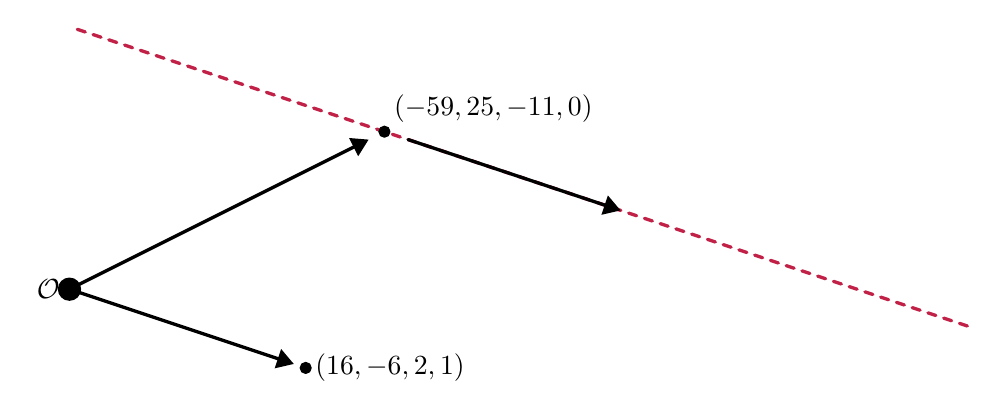
\begin{tikzpicture}[line cap=round, line join=round, >=Triangle,scale=2]
	% coordinate system
	\coordinate (O) at (0,0); 
	\coordinate (A) at (2,1); 
	\coordinate (B) at (1.5,-0.5); 
	
	% straight lines y= x/2 + 1, y=x/3 + 1 and y= -x/3 + 2
	\draw[->,very thick,black] (O)--($(O)+0.95*(A)$);
	\draw[->,very thick,black] (O)--($0.95*(B)$);
	\draw[dashed,very thick,brightmaroon] ($(A)-1.3*(B)$)--($(A)+2.5*(B)$);
	\draw[->,very thick,black] ($(A)+0.1*(B)$)--($(A)+(B)$);
	\filldraw [black] (O) circle (2pt) node[left] {$\mathcal{O}$};
	\filldraw [black] (B) circle (1pt) node[right] {$(16,-6,2,1)$};
	\filldraw [black] (A) circle (1pt) node[above right] {$(-59,25,-11,0)$};

\end{tikzpicture}
\end{center}

All the points on the red dashed line are solutions of $AX=Y$.
}



\definition{Overdetermined system}{
An overdetermined system has more equations than unknowns. We say “there are too many equations”. Such a system allows solutions only if certain conditions are met. 
}

\noindent For example, in the following figure we have 3 straight lines.

\begin{center}
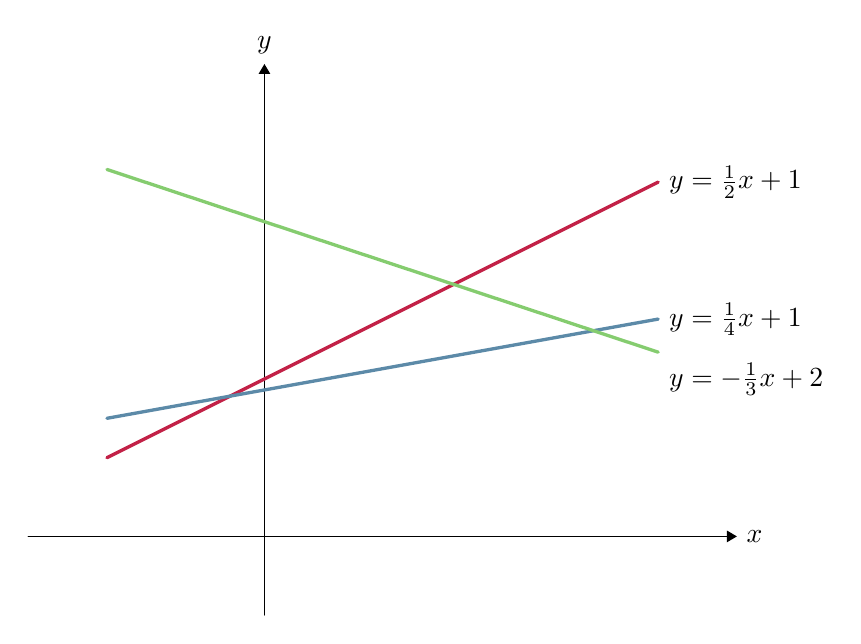
\begin{tikzpicture}[line cap=round, line join=round, >=Triangle,scale=2]
	% coordinate system
	\coordinate (O) at (0,0); 
	\draw[->] (-1.5, 0) -- (3,0) node[right] {$x$};
	\draw[->] (0, -0.5) -- (0,3) node[above] {$y$};
	
	% straight lines y= x/2 + 1, y=x/3 + 1 and y= -x/3 + 2
	\draw[-,very thick,brightmaroon] (-1,0.5)--(2.5,2.25) node[right,black] {$y= \frac{1}{2}x + 1$};
	\draw[-,very thick,airforceblue] (-1,0.75)--(2.5,1.38) node[right,black] {$y=\frac{1}{4}x + 1$};
	\draw[-,very thick,nicegreen] (-1,2.33)--(2.5,1.17) node[below right,black] {$y= -\frac{1}{3}x + 2$};

\end{tikzpicture}
\end{center}
There is nowhere that all three of these lines overlap, that is, nowhere that the three equations are simultaneously true.



\example{Overdetermined system with one solution}{
The following overdetermined system, despite have 5 equations and 4 unknowns, has exactly one solution
\begin{align*}
(S)
\left\{
\begin{matrix}
    x &  +3y &   -z &  +4t &=&   27 \\
  -4x & -11y &  +6z & -14t &=& -105 \\
  -2x & -10y &  -7z & -14t &=&  -55 \\
   2x &  +9y &  +6z &  +9t &=&   37 \\
   2x & +18y & +26z & +23t &=&   42
\end{matrix}
\right.
\end{align*}
After many lines of the usual Gaussian method, we arrive at \hspace{-0.3cm}
\begin{align*}
\left(
	\begin{matrix}
	   1 &   3 &  -1 &   4 \\
	   0 &   1 &   2 &   2 \\
	   0 &   0 &  -1 &   2 \\
	   0 &   0 &   0 & -1 \\
	   0 &   0 &   0 & -1
	\end{matrix}
  \left|
	\begin{matrix}
	    27 \\
	     3 \\
	    11 \\
	    -4 \\
	    -4
	\end{matrix}
  \right.
\right)
\end{align*}
This means we have shown an equivalence between the last two equations. The 4th row
can be subtracted from the 5th, and we solve the system as though only the 4 equations
exist. The unique solution is then $(x,y,z,t)=(5,1,-3,4)$.
}

\example{Overdetermined system with no solutions}{
The following system, same as previous with just 1 change, has no solutions
\begin{align*}
(S)
\left\{
\begin{matrix}
    x &  +3y &   -z &  +4t &=&   27 \\
  -4x & -11y &  +6z & -14t &=& -105 \\
  -2x & -10y &  -7z & -14t &=&  -55 \\
   2x &  +9y &  +6z &  +9t &=&   37 \\
   2x & +18y & +26z & +23t &=&   \colourboxed{red}{45}
\end{matrix}
\right.
\end{align*}
After many lines of the usual Gaussian method, we arrive at \hspace{-0.3cm}
\begin{align*}
\left(
	\begin{matrix}
	   1 &   3 &  -1 &   4 \\
	   0 &   1 &   2 &   2 \\
	   0 &   0 &  -1 &   2 \\
	   0 &   0 &   0 & -1 \\
	   0 &   0 &   0 & -1
	\end{matrix}
  \left|
	\begin{matrix}
	    27 \\
	     3 \\
	    11 \\
	    -4 \\
	     9
	\end{matrix}
  \right.
\right)
\end{align*}
The last two rows represent equations $t = 6$ and $t = -9$. Of course these two equations can’t be true simultaneously, so the system has no solutions.
}



\definition{Underdetermined system}{

An \textbf{underdetermined system} has less equations than unknowns. We say ``there are not enough equations''. Such a system has either no solutions, or infinitely many. 
}

For example, the equation of a plane has 3 unknowns: $ax + by + cz = d$. So a system of 2 planes is underdetermined. We could have the following two situations:
\begin{figure}[H]
\centering
\begin{subfigure}{.45\textwidth}
    \centering
    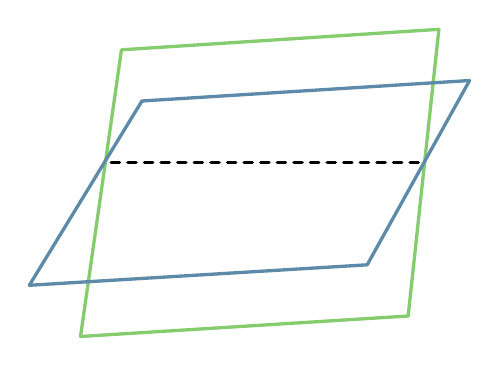
\begin{tikzpicture}[line cap=round, line join=round, >=Triangle,scale=1.3]
    	\coordinate (A1) at (0.0,0.0);
    	\coordinate (B1) at (0.4,2.8);
    	\coordinate (C1) at (3.5,3.0);
    	\coordinate (D1) at (3.2,0.2);
    	
    	\coordinate (A2) at (-0.5,0.5);
    	\coordinate (B2) at (0.6,2.3);
    	\coordinate (C2) at (3.8,2.5);
    	\coordinate (D2) at (2.8,0.7);
    	
		\draw [-,nicegreen,line width=1.2pt] (A1)--(B1);
		\draw [-,nicegreen,line width=1.2pt] (B1)--(C1);
		\draw [-,nicegreen,line width=1.2pt] (C1)--(D1);
		\draw [-,nicegreen,line width=1.2pt] (D1)--(A1);
    	
		\draw [-,airforceblue,line width=1.2pt] (A2)--(B2);
		\draw [-,airforceblue,line width=1.2pt] (B2)--(C2);
		\draw [-,airforceblue,line width=1.2pt] (C2)--(D2);
		\draw [-,airforceblue,line width=1.2pt] (D2)--(A2);

		\draw [dashed,black,line width=1.2pt] (0.3,1.7)--(3.3,1.7);
    \end{tikzpicture}
    \caption*{These 2 planes intersect at a line, the infinite points of which are the solutions to the two equations.}
\end{subfigure}
\hfill
\begin{subfigure}{.45\textwidth}
    \centering
    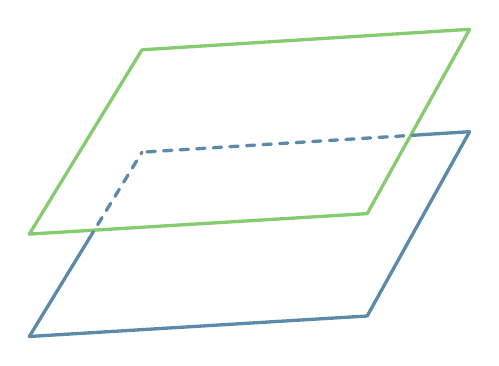
\begin{tikzpicture}[line cap=round, line join=round, >=Triangle,scale=1.3]
    	\coordinate (A1) at (-0.5,1.5);
    	\coordinate (B1) at (0.6,3.3);
    	\coordinate (C1) at (3.8,3.5);
    	\coordinate (D1) at (2.8,1.7);
    	
    	\coordinate (A2) at (-0.5,0.5);
    	\coordinate (B2) at (0.6,2.3);
    	\coordinate (C2) at (3.8,2.5);
    	\coordinate (D2) at (2.8,0.7);
    	
		\draw [-,nicegreen,line width=1.2pt] (A1)--(B1);
		\draw [-,nicegreen,line width=1.2pt] (B1)--(C1);
		\draw [-,nicegreen,line width=1.2pt] (C1)--(D1);
		\draw [-,nicegreen,line width=1.2pt] (D1)--(A1);
    	
		\draw [-,airforceblue,line width=1.2pt] (A2)--($0.47*(A2)+0.53*(B2)$);
		\draw [dashed,airforceblue,line width=1.2pt] ($0.47*(A2)+0.53*(B2)$)--(B2);
		\draw [-,airforceblue,line width=1.2pt] (C2)--($0.85*(C2)+0.15*(B2)$);
		\draw [dashed,airforceblue,line width=1.2pt] ($0.85*(C2)+0.15*(B2)$)--(B2);
		\draw [-,airforceblue,line width=1.2pt] (C2)--(D2);
		\draw [-,airforceblue,line width=1.2pt] (D2)--(A2);
    \end{tikzpicture}
    \caption*{These 2 planes are simply offset and never intersect. Hence there are no solutions.}
\end{subfigure}
\end{figure}


\example{Undetermined system with infinite solutions}{
Consider the following \textbf{underdetermined system}
\begin{align*}
(S)
\left\{
\begin{matrix}
    x &  +3y &   -z &  +4t &=&   27 \\
  -4x & -11y &  +6z & -14t &=& -105 \\
  -2x & -10y &  -7z & -14t &=&  -55
\end{matrix}
\right.
\end{align*}
After some lines of the usual Gaussian method, we arrive at 
\begin{align*}
\left(
	\begin{matrix}
	   1 &   3 &  -1 &   4 \\
	   0 &   1 &   2 &   2 \\
	   0 &   0 &  -1 &   2
	\end{matrix}
  \left|
	\begin{matrix}
	    27 \\
	     3 \\
	    11 \\
	\end{matrix}
  \right.
\right)
\end{align*}
We already solved this system. The infinite solutions are:
\begin{align*}
\begin{pmatrix}
   x \\
   y \\
   z \\
   t
\end{pmatrix}
=
\begin{pmatrix}
   16t - 59 \\
   -6t + 25\\
    2t - 11\\
     t
\end{pmatrix}
=
\begin{pmatrix}
   16 \\
    -6 \\
   2\\
   1
\end{pmatrix}
t
+
\begin{pmatrix}
   -59 \\
    25 \\
   -11 \\
     0
\end{pmatrix}
\end{align*}
}



\section{Cramer systems and Cramer's rule}



\definition{Cramer system}{
Suppose we have the following linear system of equations (with unknowns equal to equations)
\begin{align*}
\begin{cases}
a_{11} x_1  + a_{12} x_2 + \cdots + a_{1n} x_n = y_1 \\
a_{21} x_1  + a_{22} x_2 + \cdots + a_{2n} x_n = y_2 \\
\vdots \\
a_{n1} x_1  + a_{n2} x_2 + \cdots + a_{nn} x_n = y_n
\end{cases}
\qquad (S)
\end{align*}
with the associated matrix form
\begin{align*}
\underbrace{
\begin{pmatrix}
a_{11} & a_{12} & \cdots & a_{1n} \\
a_{21} & a_{22} & \cdots & a_{2n} \\
\vdots & \vdots & \ddots & \vdots \\
a_{n1} & a_{n2} & \cdots & a_{nn}
\end{pmatrix}}_A
%%
%%
\underbrace{
\begin{pmatrix}
x_{1} \\
x_{2} \\
\vdots \\
x_{n}
\end{pmatrix}}_X
%%
=
\underbrace{
\begin{pmatrix}
y_{1} \\
y_{2} \\
\vdots \\
y_{n}
\end{pmatrix}}_Y
\end{align*}
We say that $(S)$ is a Cramer system if $\det(A) \neq 0$.
}

\theorem{Cramer's rule}{
The unique solution to a Cramer system, $X$, has coefficients given by Cramer's rule:
\begin{align*}
x_i = \dfrac{1}{\det(A)}
\underbrace{
\left|
\begin{matrix}
a_{11} & \cdots & a_{1,i-1} & y_1 & a_{1,i+1} & \cdots & a_{1n} \\
a_{21} & \cdots & a_{2,i-1} & y_2 & a_{2,i+1} & \cdots & a_{2n} \\
\vdots & \cdots & \vdots    & \vdots & \vdots & \ddots & \vdots \\
a_{n1} & \cdots & a_{n,i-1} & y_n & a_{n,i+1} & \cdots & a_{nn}
\end{matrix}
\right|
}_{\text{Replace the ith column with Y}}
\quad \text{for every $i$}
\end{align*}

Note that this means we must take $n$ different determinants of this style, one for each unknown in the $X$ column.
}


\example{Cramer's rule}{

Let's use Cramer’s rule to find the solutions to the system $(S)$ with the following associated coefficient matrices and constant columns
\begin{align*}
A =& 
\begin{pmatrix}
3 & 1 & 5 \\
2 & 1 & 2 \\
0 & 3 & 7 
\end{pmatrix}
\quad
Y = 
\begin{pmatrix}
2 \\ 1 \\ 3
\end{pmatrix}
\qquad (S)
\end{align*}
We first need the determinant of the matrix
\begin{align*}
\det(A) = 3\left| \begin{matrix} 1 & 2 \\ 3 & 7 \end{matrix} \right|
- 2\left| \begin{matrix} 1 & 5 \\ 3 & 7 \end{matrix} \right|
= 3(7-6) - 2(7-15) = 19
\end{align*}
Then we apply Cramer's rule to find each of the three solution coefficients:
\begin{align*}
x_1 &= \frac{1}{\det(A)}
  \left|\begin{array}{>{\columncolor{airforceblue!20}}ccc}
	2 & 1 & 5 \\
	1 & 1 & 2 \\
	3 & 3 & 7 
  \end{array}\right|
  = \frac{1}{19}\left(
  	  2\left|\begin{matrix} 1 & 2 \\ 3 & 7 \end{matrix}\right| 
  	 -5\left|\begin{matrix} 1 & 2 \\ 3 & 7 \end{matrix}\right|
  	 +5\left|\begin{matrix} 1 & 1 \\ 3 & 3 \end{matrix}\right|
  	\right)
  = \frac{1}{19}
%%
\\
%%
x_2 &= \frac{1}{\det(A)}
  \left|\begin{array}{c>{\columncolor{airforceblue!20}}cc}
	3 & 2 & 5 \\
	2 & 1 & 2 \\
	0 & 3 & 7 
  \end{array}\right|
  = \frac{1}{19}\left(
  	  3\left|\begin{matrix} 1 & 2 \\ 3 & 7 \end{matrix}\right| 
  	 -2\left|\begin{matrix} 2 & 2 \\ 0 & 7 \end{matrix}\right|
  	 +5\left|\begin{matrix} 2 & 1 \\ 0 & 3 \end{matrix}\right|
  	\right)
  = \frac{5}{19}\vspace{-0.5cm}
%%
\\
%%
x_3 &= \frac{1}{\det(A)}
  \left|\begin{array}{cc>{\columncolor{airforceblue!20}}c}
	3 & 1 & 2 \\
	2 & 1 & 1 \\
	0 & 3 & 3 
  \end{array}\right|
  = \frac{1}{19}\left(
  	  3\left|\begin{matrix} 1 & 1 \\ 3 & 3 \end{matrix}\right| 
  	 -1\left|\begin{matrix} 2 & 1 \\ 0 & 3 \end{matrix}\right|
  	 +2\left|\begin{matrix} 2 & 1 \\ 0 & 3 \end{matrix}\right|
  	\right)
  = \frac{6}{19}
\end{align*}
So the unique solution to $(S)$ is $(x_1,x_2,x_3)=\dfrac{1}{19}(1,5,6)$
}
%%%%%%%%%%%%%%%%%%%%%%%%%%%%%%%%%%%%%%%%%%%%%%%%%%%%%%%%%%%%%%%%%%%%%%%%

%\end{document}

\pagenumbering{roman}

\thispagestyle{empty}
\begin{titlepage}

\newcommand{\HRule}{\rule{\linewidth}{0.5mm}} % Defines a new command for the horizontal lines, change thickness here

\center % Center everything on the page
 
%----------------------------------------------------------------------------------------
%	HEADING SECTIONS
%----------------------------------------------------------------------------------------

%\textsc{\LARGE Macquarie University}\\[1.5cm] % Name of your university/college
%\textsc{\Large Honours Thesis}\\[0.5cm] % Major heading such as course name



%----------------------------------------------------------------------------------------
%	DATE SECTION
%----------------------------------------------------------------------------------------
%\includegraphics[width=1.0\textwidth]{Front2.jpg}\\[1.0cm]

%----------------------------------------------------------------------------------------
%	TITLE SECTION
%----------------------------------------------------------------------------------------

\HRule \\[0.4cm]
{ \huge \bfseries Incomplete Notes On}\\[0.4cm] % Title of your document
{ \huge \bfseries Numerical Methods} % Title of your document
\HRule \\[0.2cm]
 
%----------------------------------------------------------------------------------------
%	AUTHOR SECTION
%----------------------------------------------------------------------------------------



\begin{minipage}{0.4\textwidth}
\begin{flushleft} \large
\centering Andrew Lehmann \\
\centering \today \\
\end{flushleft}
\end{minipage}

\vfill

\begin{figure}[H]
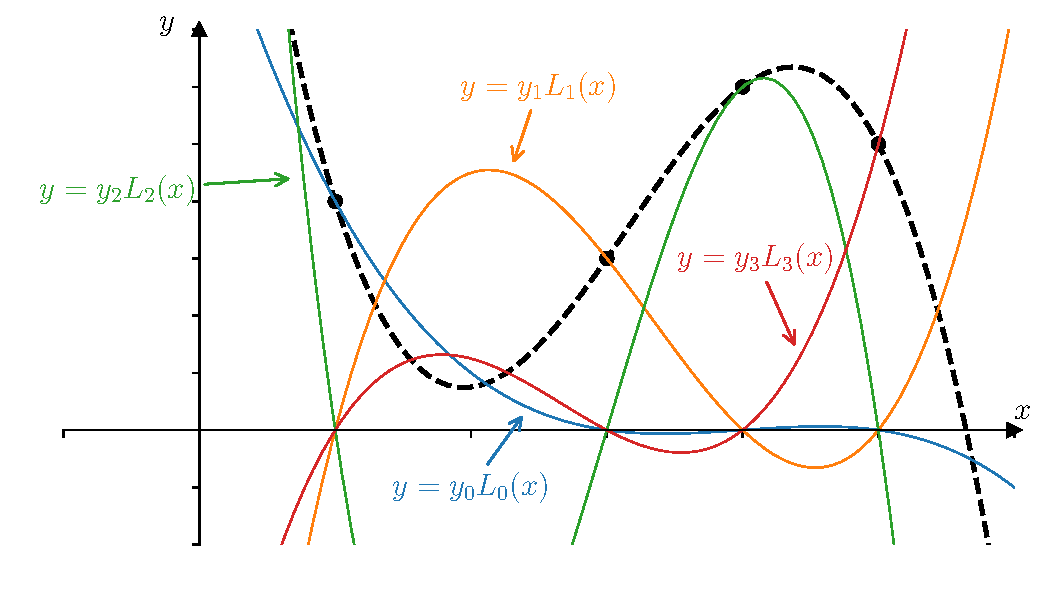
\includegraphics[width=\textwidth]{figures/ch3_lagrange_total.pdf}
\end{figure}

\vfill % Fill the rest of the page with whitespace

\begin{center}
Typeset in \LaTeXe.
\end{center}
\end{titlepage}


\onehalfspacing


\addcontentsline{toc}{chapter}{\bf Contents}
\tableofcontents

\clearpage

% List of Definitions and Theorems
%\listoftheorems[ignoreall]
\renewcommand{\listtheoremname}{List of Definitions}
\listoftheorems[ignoreall,show=definitionnew]
\renewcommand{\listtheoremname}{List of Theorems}
\listoftheorems[ignoreall,show=theoremnew]

\clearpage
\pagenumbering{arabic}
\chapter{Euclidean Vectors} \label{ch:euclid}

\section{Basic definitions}

\definition{Euclidean vector or tuple}{
A Euclidean vector is a list of $n$ real numbers, also called an $n$-tuple. We write this list in parentheses, for example $(1,3,-2, \dots, 0)$, and we say that this object belongs to $\mathbb{R}^n$. An arbitrary tuple can be written $\mathbf{v}=(v_1,v_2,\cdots,v_n)$ where the \textit{components} $v_i \in \mathbb{R}$ for any index $i$.
}

\noindent It will be particularly useful to build intuition on vectors in $\mathbb{R}^2$. These are pairs of numbers like $(1,2)$, $(-1,\pi)$ etc. We represent these vectors on a cartesian plane by associating an arrow pointing from the origin, $\mathcal{O}=(0,0)$, to the given pair of numbers $(x,y)$ as below

\begin{figure}[H]
\centering
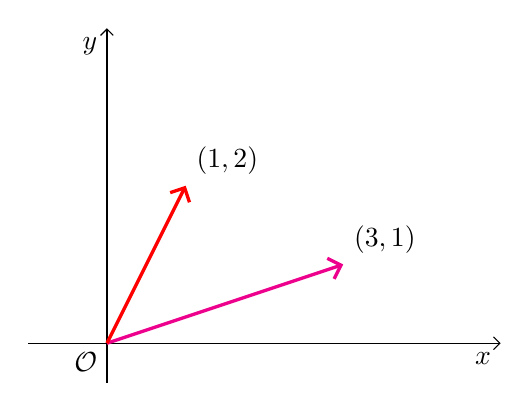
\begin{tikzpicture}[% styles used in image code
         > = Straight Barb, % defined in "arrows.meta
dot/.style = {circle, fill,
              minimum size=2mm, inner sep=0pt, outer sep=0pt,
              node contents={}},
box/.style = {draw, thin, minimum  width=2mm, minimum height=4mm,
              inner sep=0pt, outer sep=0pt,
              node contents={}, sloped},
my angle/.style args = {#1/#2}{draw,->,
                               angle radius=#1,
                               angle eccentricity=#2,
                               } % angle label position!
                        ]
	% coordinate axis
	\draw[->] (-1, 0)   -- (5,0) node[below left] {$x$};
	\draw[->] ( 0,-0.5) -- (0,4) node[below left] {$y$};

	\coordinate (O) at (0,0);
	\coordinate (v1) at (3,1);
	\coordinate (v2) at (1,2);
	
	\draw (O) node[below left] {$\mathcal{O}$};
	\draw [->,magenta,very thick] (O) --(v1) node[above right,black] {$(3,1)$};
	\draw [->,red,very thick] (O) --(v2) node[above right,black] {$(1,2)$};
\end{tikzpicture} \caption*{Arrow representation of two euclidean vectors.}
\end{figure}

\noindent The components of euclidean vectors represented this way are generally called the $x$ and $y$ components (there will be a $z$ component for triples), and so we often write $\mathbf{v}=(v_x, v_y)$. For obvious reasons we also call these 2 dimensional vectors.

Now we would like to create a way to add vectors together. When we add two vectors together the result should also be a vector. 

\definition{Tuple addition}{
Euclidean vectors are added to each other component by component. In symbols
\begin{align*}
(a_1, a_2, \dots, a_n) + (b_1, b_2, \dots, b_n) = (a_1+b_1, a_2+b_2, \dots, a_n + b_n).
\end{align*}
\textit{Note}: this means you can only add two tuples together \textit{of the same size}. It makes no sense to add a 3-tuple to a 5-tuple.
}

\noindent Let's understand this tuple addition geometrically. For the two vectors we represented above, $\mathbf{a}=(1,2)$, $\mathbf{b}=(3,1)$ and so their addition is the vector $\mathbf{c}=\mathbf{a}+\mathbf{b}=(1+3,2+1)=(4,3)$. This component by component addition is represented below left. We can also understand this addition as though we move the vector $\mathbf{b}$ so that its tail is at the tip of $\mathbf{a}$. This tip-to-tail method is shown below to the right. It equally works by moving $\mathbf{a}$ to the tip of $\mathbf{b}$ meaning that $\mathbf{a}+\mathbf{b} = \mathbf{b}+\mathbf{a}$.

\begin{figure}[H]
\centering
\begin{subfigure}[b]{0.45\textwidth}
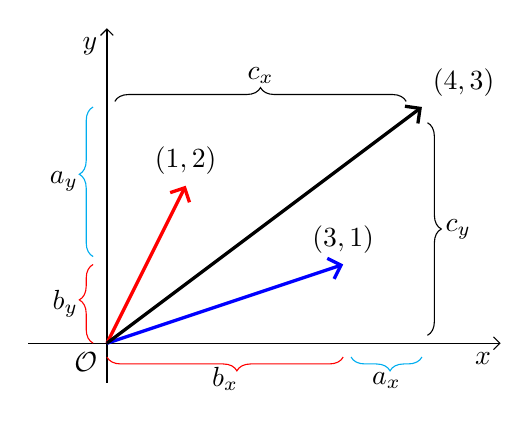
\begin{tikzpicture}[% styles used in image code
         > = Straight Barb, % defined in "arrows.meta
dot/.style = {circle, fill,
              minimum size=2mm, inner sep=0pt, outer sep=0pt,
              node contents={}},
box/.style = {draw, thin, minimum  width=2mm, minimum height=4mm,
              inner sep=0pt, outer sep=0pt,
              node contents={}, sloped},
my angle/.style args = {#1/#2}{draw,->,
                               angle radius=#1,
                               angle eccentricity=#2,
                               } % angle label position!
                        ]
	% coordinate axis
	\draw[->] (-1, 0)   -- (5,0) node[below left] {$x$};
	\draw[->] ( 0,-0.5) -- (0,4) node[below left] {$y$};

	\coordinate (O) at (0,0);
	\coordinate (a) at (1,2);
	\coordinate (ax) at (1,0);
	\coordinate (ay) at (0,2);
	\coordinate (b) at (3,1);
	\coordinate (bx) at (3,0);
	\coordinate (by) at (0,1);
	\coordinate (c) at (4,3);
	\coordinate (cx) at (4,0);
	\coordinate (cy) at (0,3);
	
	\draw (O) node[below left] {$\mathcal{O}$};
	\draw [->,red,very thick] (O) -- (a) node[black, above] {$(1,2)$};
	\draw [->,blue,very thick]  (O) -- (b) node[black, above] {$(3,1)$};
	\draw [->,very thick] (O) -- (c) node[above right] {$(4,3)$};
	
	
	\draw [black, decorate, decoration={brace,amplitude=5pt,raise=2pt,aspect=0.5}] 
		($(cy)+(0.1,0)$)--($(c)-(0.2,0)$) node[pos=0.5,black,above=5pt]{$c_x$};
	\draw [black, decorate, decoration={brace,mirror,amplitude=5pt,raise=2pt,aspect=0.5}] 
		($(cx)+(0,0.1)$) -- ($(c)-(0,0.2)$) node[pos=0.5,black,right=5pt]{$c_y$};
	
	\draw [red, decorate, decoration={brace,mirror,raise=5pt,amplitude=5pt,aspect=0.55}] 
		(O)--(bx) node[pos=0.5,black,below=5pt]{$b_x$};
	
	\draw [red, decorate, decoration={brace,raise=5pt,amplitude=5pt,aspect=0.55}] 
		(O)--(by) node[pos=0.5,black,left=7pt]{$b_y$};
	
	\draw [cyan, decorate, decoration={brace,mirror,raise=5pt,amplitude=5pt,aspect=0.55}] 
		($(bx)+(0.1,0)$)--($(bx)+(ax)$) node[pos=0.5,black,below=7pt]{$a_x$};
	
	\draw [cyan, decorate, decoration={brace,raise=5pt,amplitude=5pt,aspect=0.55}] 
		($(by)+(0,0.1)$)--($(by)+(ay)$) node[pos=0.5,black,left=7pt]{$a_y$};
		
\end{tikzpicture} \caption*{Component by component addition.}
\end{subfigure}
~
\begin{subfigure}[b]{0.45\textwidth}
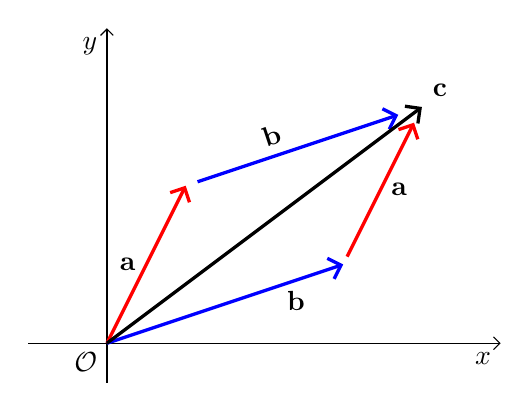
\begin{tikzpicture}[% styles used in image code
         > = Straight Barb, % defined in "arrows.meta
dot/.style = {circle, fill,
              minimum size=2mm, inner sep=0pt, outer sep=0pt,
              node contents={}},
box/.style = {draw, thin, minimum  width=2mm, minimum height=4mm,
              inner sep=0pt, outer sep=0pt,
              node contents={}, sloped},
my angle/.style args = {#1/#2}{draw,->,
                               angle radius=#1,
                               angle eccentricity=#2,
                               } % angle label position!
                        ]
	% coordinate axis
	\draw[->] (-1, 0)   -- (5,0) node[below left] {$x$};
	\draw[->] ( 0,-0.5) -- (0,4) node[below left] {$y$};

	\coordinate (O) at (0,0);
	\coordinate (a) at (1,2);
	\coordinate (b) at (3,1);
	\coordinate (c) at (4,3);
	
	\draw (O) node[below left] {$\mathcal{O}$};
	\draw [->,red,very thick] (O) --(a) node[black,pos=0.5,left] {$\mathbf{a}$};
	\draw [->,blue,very thick] ($(a)+0.05*(b)$) --($(a)+0.9*(b)$) node[black,pos=0.4,rotate=18.4,above] {$\mathbf{b}$};
	\draw [->,blue,very thick] (O) --(b) node[black,pos=0.8,below] {$\mathbf{b}$};
	\draw [->,red,very thick] ($(b)+0.05*(a)$) --($(b)+0.9*(a)$) node[black,pos=0.5,pos=0.5,right] {$\mathbf{a}$};
	\draw [->,very thick] (O) --(c) node[above right] {$\mathbf{c}$};
\end{tikzpicture} \caption*{Tip-to-tail representation.}
\end{subfigure}
\end{figure}

\noindent Now lets think about multiplcation. We can naturally think of doubling or tripling a vector, which should be adding a vector to itself 2 or 3 times, and geometrically it just becomes longer. So we want $2\mathbf{v} = \mathbf{v} + \mathbf{v}$. In components this gives $2(v_x,v_y)=(v_x,v_y) + (v_x,v_y) = (2v_x,2v_y)$. So we see that multiplying a tuple by a number multiplies each of its components by that number.

\definition{Scalar multiplication}{
Let $c\in\mathbb{R}$, called a scalar quantity, and $\mathbf{v} \in \mathbb{R}^n$ with components $v_i$. Then the \textit{scalar multiplication} $c\mathbf{v}$ gives a vector $\mathbf{w}$ with components $w_i = c v_i$ for every index $i$. In tuple form
\begin{align*}
c(v_1,v_2,\dots,v_n) = (cv_1,cv_2,\dots,cv_n).
\end{align*}
}

\begin{figure}[H]
\centering
\begin{tikzpicture}[% styles used in image code
         > = Straight Barb, % defined in "arrows.meta
dot/.style = {circle, fill,
              minimum size=2mm, inner sep=0pt, outer sep=0pt,
              node contents={}},
box/.style = {draw, thin, minimum  width=2mm, minimum height=4mm,
              inner sep=0pt, outer sep=0pt,
              node contents={}, sloped},
my angle/.style args = {#1/#2}{draw,->,
                               angle radius=#1,
                               angle eccentricity=#2,
                               } % angle label position!
                        ]
	% coordinate axis
	\draw[->] (-3, 0)   -- (5,0) node[below left] {$x$};
	\draw[->] ( 0,-1) -- (0,3) node[below left] {$y$};

	\coordinate (O) at (0,0);
	\coordinate (v1) at (2,1);
	\coordinate (v2) at (1,0.5);
	\coordinate (v3) at (4,2);
	\coordinate (v4) at (-2,-1);
	
	\draw (O) node[below right] {$\mathcal{O}$};
	\draw [->,blue] (O) --(v3) node[pos=0.7,above,black] {$2\mathbf{v}$};
	\draw [->,black] (O) --(v1) node[pos=0.78,above,black] {$\mathbf{v}$};
	\draw [->,magenta,very thick] (O) --(v2) node[pos=0.5,above=5pt,black] {$0.5\mathbf{v}$};
	\draw [->,red] (O) --(v4) node[pos=0.7,above,black] {$-1\mathbf{v}$};
\end{tikzpicture} \caption*{Arrow representation of scalar multiplication.}
\end{figure}

\noindent We can use scalar multiplication and some manipulation to form a second way to represent Euclidean vectors:
\begin{align*}
(v_1,v_2,\dots,v_n) &= (v_1,0,\dots,0) + (0,v_2,\dots,0) + \cdots + (0,0,\dots,v_n) \\
&= v_1(1,0,\dots,0) + v_2(0,1,\dots,0) + \cdots + v_n(0,0,\dots,1)\\
&= v_1\mathbf{e}_1 + v_2\mathbf{e}_2 + \cdots + v_n\mathbf{e}_n
\end{align*}
where we have introduced the canonical Euclidean vectors.

\definition{Canonical Euclidean unit vectors}{
The canonical Euclidean vectors in $\mathbb{R}^n$ are the $n$ vectors of the form
\begin{gather*}
\mathbf{e}_1 = (1,0,\dots,0) \\
\mathbf{e}_2 = (0,1,\dots,0) \\
\vdots \\
\mathbf{e}_n = (0,0,\dots,1).
\end{gather*}
More compactly
\begin{align*}
\mathbf{e}_k = (\alpha_1, \alpha_2, \dots, \alpha_n) \quad \text{where} \quad
\alpha_j=
\begin{cases}
1 & \text{for } j= k, \\
0 & \text{for } j\neq k.
\end{cases}
\end{align*}
}

\noindent In two dimensions we have several notations for these unit vectors
\begin{align*}
\mathbf{v} = v_x \hat{x} + v_y \hat{y} = v_x \mathbf{e}_x + v_y \mathbf{e}_y = v_x \hat{i} + v_y \hat{j}
\end{align*}
but we will stick to the hat notation, $\hat{x}$, in this text when referring to the geometric representations in 2 or 3d ($\hat{z}=\mathbf{e}_z = \hat{k}$ being used for the third direction). We can understand these unit vectors as the building blocks of the arrow:
\begin{figure}[H]
\centering
\begin{tikzpicture}[% styles used in image code
         > = Straight Barb, % defined in "arrows.meta
dot/.style = {circle, fill,
              minimum size=2mm, inner sep=0pt, outer sep=0pt,
              node contents={}},
box/.style = {draw, thin, minimum  width=2mm, minimum height=4mm,
              inner sep=0pt, outer sep=0pt,
              node contents={}, sloped},
my angle/.style args = {#1/#2}{draw,->,
                               angle radius=#1,
                               angle eccentricity=#2,
                               } % angle label position!
                        ]
	% coordinate axis
	\draw[->] (-3, 0)   -- (5,0) node[below] {$x$};
	\draw[->] ( 0,-1) -- (0,3.5) node[left] {$y$};

	\coordinate (O) at (0,0);
	\coordinate (v) at (2,3);
	\coordinate (xhat) at (1,0);
	\coordinate (yhat) at (0,1);
	
	\draw (O) node[below left] {$\mathcal{O}$};
	\draw [->] (O) --(v) node[pos=0.9,above left,rotate=56.3] {$\mathbf{v}=(2,3)$};
	\draw [->, blue] (O) --(xhat) node[pos=0.5,below=5pt] {$\hat{x}$};
	\draw [->, blue] (xhat) --($2*(xhat)$) node[pos=0.5,below=5pt] {$\hat{x}$};
	\draw [->, magenta] (O) --(yhat) node[pos=0.5,left=5pt] {$\hat{y}$};
	\draw [->, magenta] ($2*(xhat)$) --($2*(xhat)+(yhat)$) node[pos=0.5,right=5pt] {$\hat{y}$};
	\draw [->, magenta] ($2*(xhat)+(yhat)$) --($2*(xhat)+2*(yhat)$) node[pos=0.5,right=5pt] {$\hat{y}$};
	\draw [->, magenta] ($2*(xhat)+2*(yhat)$) --($2*(xhat)+3*(yhat)$) node[pos=0.5,right=5pt] {$\hat{y}$};
\end{tikzpicture} \caption*{Unit vectors as building blocks of a Euclidean vector.}
\end{figure}

\section{Dot product}

\noindent Notice that with scalar multiplication we multiplied two different kinds of objects together, a scalar by a vector resulting in a vector. How about multiplying two vectors together? You might be tempted to simply form a new vector with component by component multiplication, as we did for addition. This turns out not to be so useful. One very useful way to define vector multiplication is as follows.

\definition{Dot product}{
For two $n$-tuples $\mathbf{a}$ and $\mathbf{b}$, their \textit{dot product}, also called \textit{scalar} product and \textit{Euclidean inner} product, is the real number given by the addition of component by component multiplication
\begin{align*}
\mathbf{a}\cdot\mathbf{b} = a_1 b_1 + a_2 b_2 + \cdots + a_n b_n = \sum_{i=1}^n a_i b_i.
\end{align*}
}

\noindent Notice that the result of this product is a real number, not another tuple. Let's first try to understand the dot product by considering a 2d vector ``dotted'' with itself:
\begin{align*}
\mathbf{v}\cdot\mathbf{v}=(v_x,v_y)\cdot(v_x,v_y)=v_x^2 + v_y^2.
\end{align*}
This dot product gives the square of the length of the right triangle made from the $x$ and $y$ components of $\mathbf{v}$:

\begin{figure}[H]
\centering
\begin{tikzpicture}[% styles used in image code
         > = Straight Barb, % defined in "arrows.meta
dot/.style = {circle, fill,
              minimum size=2mm, inner sep=0pt, outer sep=0pt,
              node contents={}},
box/.style = {draw, thin, minimum  width=2mm, minimum height=4mm,
              inner sep=0pt, outer sep=0pt,
              node contents={}, sloped},
my angle/.style args = {#1/#2}{draw,->,
                               angle radius=#1,
                               angle eccentricity=#2,
                               } % angle label position!
                        ]
	% coordinate axis
	%\draw[->] (-3, 0)   -- (5,0) node[below left] {$x$};
	%\draw[->] ( 0,-1) -- (0,3) node[below left] {$y$};

	\coordinate (O) at (0,0);
	\coordinate (v1) at (6,4);
	\coordinate (vx) at (6,0);
	\coordinate (vy) at (0,4);
	
	\draw [->] (O) --(v1) node[pos=0.5,above=5pt] {$\mathbf{v}$};
	\draw [dashed] (O) --($(vx)-(0.1,0)$) node[pos=0.5,below] {$v_x$};
	\draw [dashed] (vx) --($(v1)-(0,0.15)$) node[pos=0.5,right] {$v_y$};
\end{tikzpicture} \caption*{Components of the vector $\mathbf{v}$}
\end{figure}

\noindent So we can identify the dot product $\mathbf{v}\cdot\mathbf{v}$ with the square of the length of $\mathbf{v}$. We generalise this concept of vector length in the operation of the norm.

\definition{Norm}{
The norm of an $n$-tuple $\mathbf{v}$, denoted $\lVert \mathbf{v} \rVert$, is given by
\begin{align*}
\lVert \mathbf{v} \rVert = \sqrt{\mathbf{v}\cdot\mathbf{v}} = \sqrt{v_1^2 + v_2^2 + \cdots + v_2^2}.
\end{align*}
}

\noindent So far we have defined a vector by its components. Through the norm, we can have a method of \textit{calculating} the components from 2 other pieces of information: its length and its direction. Its direction will mean its angle with respect to the $x$-axis. Denote that angle $\theta$ and the norm as the non-bold font version of the vector $v=\lVert \mathbf{v} \rVert$. From the above figure, we see that $\cos\theta = v_x/v$ and $\sin\theta = v_y/v$. So, given a vector length and its direction we have
\begin{align*}
\mathbf{v} = (v\cos\theta, v\sin\theta) = v(\cos\theta,\sin\theta).
\end{align*}
This gives us the following result: for any 2d Euclidean vector $\mathbf{v}$ its components are given by
\begin{align*}
v_x &= \lVert \mathbf{v} \rVert \cos\theta \\
v_y &= \lVert \mathbf{v} \rVert \sin\theta
\end{align*}
where $\theta$ is the angle that $\mathbf{v}$ makes with the $x$ axis.

\noindent What happens if we dot two different vectors with this representation. Let $\mathbf{a}=a(\cos\alpha,\sin\alpha)$ and $\mathbf{b}=b(\cos\beta,\sin\beta)$. Then
\begin{align*}
\mathbf{a}\cdot\mathbf{b} &= [a(\cos\alpha,\sin\alpha)]\cdot [b(\cos\beta,\sin\beta)] \\
&= ab(\cos\alpha,\sin\alpha)\cdot (\cos\beta,\sin\beta) \\
&= ab(\cos\alpha\cos\beta + \sin\alpha\sin\beta) \\
&= ab \cos(\alpha-\beta)
\end{align*}
where we have used a trigonometric identity in the last line and a little trickery in the first line that you should verify: $(c_1\mathbf{v}_1)\cdot(c_2\mathbf{v}_2)=(c_1c_2)\mathbf{v}_1\cdot\mathbf{v}_2$. In the end we have shown the following theorem.

\theorem{Dot product with angle}{
The Euclidean dot product of two $n$-tuples $\mathbf{a}$ and $\mathbf{b}$ can be calculated solely from their norms and the angle between them, $\theta$, given by the formula
\begin{align*}
\mathbf{a}\cdot\mathbf{b} = \lVert \mathbf{a} \rVert \lVert \mathbf{b} \rVert \cos \theta
\end{align*}
}
\begin{figure}[H]
\centering
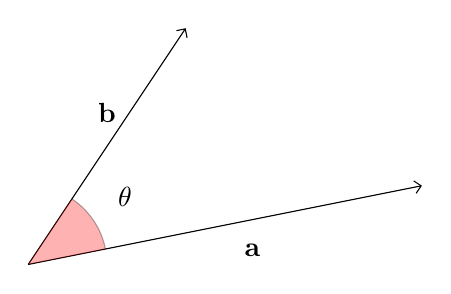
\begin{tikzpicture}[% styles used in image code
         > = Straight Barb, % defined in "arrows.meta
dot/.style = {circle, fill,
              minimum size=2mm, inner sep=0pt, outer sep=0pt,
              node contents={}},
box/.style = {draw, thin, minimum  width=2mm, minimum height=4mm,
              inner sep=0pt, outer sep=0pt,
              node contents={}, sloped},
my angle/.style args = {#1/#2}{draw,->,
                               angle radius=#1,
                               angle eccentricity=#2,
                               } % angle label position!
                        ]
	% coordinate axis
	%\draw[->] (-3, 0)   -- (5,0) node[below left] {$x$};
	%\draw[->] ( 0,-1) -- (0,3) node[below left] {$y$};

	\coordinate (O) at (0,0);
	\coordinate (a) at (5,1);
	\coordinate (b) at (2,3);
	
	\draw [->] (O) --(a) node[pos=0.5,below right=5pt] {$\mathbf{a}$};
	\draw [->] (O) --(b) node[pos=0.5,above=5pt] {$\mathbf{b}$};
	
	\begin{scope}
	\path[clip] (O) -- (a) -- (b);
	\fill[red, opacity=0.3, draw=black] (O) circle (10mm);
	\node at ($(O)+(35:15mm)$) {$\theta$};
	\end{scope}
\end{tikzpicture}\caption*{The angle between two vectors.}
\end{figure}

\noindent From this expression of the dot product we see immediately what happens in the special case of perpendicular vectors. When two vectors are perpendicular the angle between them is $\pi/2$ and the dot product is then zero (recall that $\cos(\pi/2)=0$). We can extend this result to define orthogonality for higher dimensional Euclidean vectors.

\definition{Orthogonal Euclidean vectors}{
Two vectors in $\mathbb{R}^n$ are orthogonal if and only if their dot product equals zero.
}

\section{Applications}

So far we have been considering Euclidean vectors as arrows pointing from the origin to the given tuple. It can be useful to consider arrows pointing from an arbitrary point in space to another.

\definition{Displacement vector}{
Given two Euclidean vectors $\mathbf{a}$ and $\mathbf{b}$, the displacement vector pointing from $\mathbf{a}$ to $\mathbf{b}$ is given by $\mathbf{r}=\mathbf{b}-\mathbf{a}$ as pictured below. Of course we can also create the displacement vector in the other direction, from $\mathbf{b}$ to $\mathbf{a}$, given by $\mathbf{a}-\mathbf{b}$.
}

\begin{figure}[H]
\centering
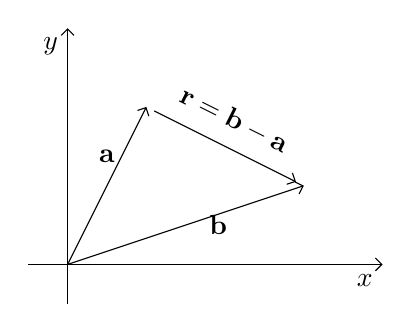
\begin{tikzpicture}[% styles used in image code
         > = Straight Barb, % defined in "arrows.meta
dot/.style = {circle, fill,
              minimum size=2mm, inner sep=0pt, outer sep=0pt,
              node contents={}},
box/.style = {draw, thin, minimum  width=2mm, minimum height=4mm,
              inner sep=0pt, outer sep=0pt,
              node contents={}, sloped},
my angle/.style args = {#1/#2}{draw,->,
                               angle radius=#1,
                               angle eccentricity=#2,
                               } % angle label position!
                        ]
	% coordinate axis
	\draw[->] (-0.5, 0) -- (4,0) node[below left] {$x$};
	\draw[->] ( 0,-0.5) -- (0,3) node[below left] {$y$};

	\coordinate (O) at (0,0);
	\coordinate (a) at (1,2);
	\coordinate (b) at (3,1);
	\coordinate (ar) at ($0.95*(a)+0.05*(b)$);
	\coordinate (br) at ($0.95*(b)+0.05*(a)$);
	
	\draw [->] (O) --(a) node[pos=0.5,above=5pt] {$\mathbf{a}$};
	\draw [->] (O) --(b) node[pos=0.5,right=5pt] {$\mathbf{b}$};
	\draw [->] (ar) --(br) node[pos=0.5,above=3pt,rotate=-26.5] {$\mathbf{r}= \mathbf{b}-\mathbf{a}$};
\end{tikzpicture}
\end{figure}

Why is this useful? Well we can, for example, represent straight lines in a new way. Recall the equation for a straight line $y=mx+b$ where $m$ gives the slope of the line and $b$ gives the $y$-intercept (or vertical offset). Let's consider the line $y=(0.5)x+1$. Now that means we can choose any two $x$ values, say $x=-1$ and $x=2$, and compute corresponding $y$ values, in this case $y=0.5$ and $y=2$. So the Euclidean vectors $\mathbf{a}=(-1,0.5)$ and $\mathbf{b}=(2,2)$ belong to the line, as pictured.

\begin{figure}[H]
\centering
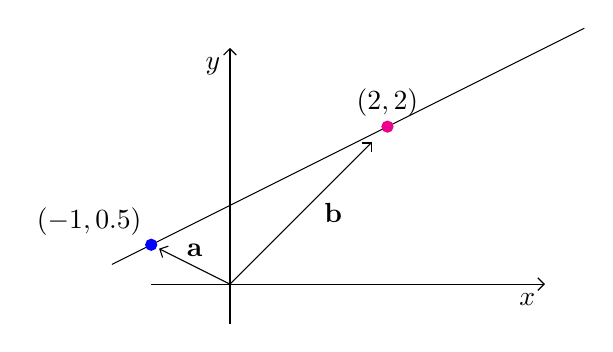
\begin{tikzpicture}[% styles used in image code
         > = Straight Barb, % defined in "arrows.meta
dot/.style = {circle, fill,
              minimum size=2mm, inner sep=0pt, outer sep=0pt,
              node contents={}},
box/.style = {draw, thin, minimum  width=2mm, minimum height=4mm,
              inner sep=0pt, outer sep=0pt,
              node contents={}, sloped},
my angle/.style args = {#1/#2}{draw,->,
                               angle radius=#1,
                               angle eccentricity=#2,
                               } % angle label position!
                        ]
	% coordinate axis
	\draw[->] (-1, 0) -- (4,0) node[below left] {$x$};
	\draw[->] ( 0,-0.5) -- (0,3) node[below left] {$y$};
	
	\draw[domain=-1.5:4.5,variable=\x] plot({\x},{0.5*\x+1});

	\coordinate (O) at (0,0);
	\coordinate (a) at (-1,0.5);
	\coordinate (b) at (2,2);
	
	\draw [->] (O) --($0.9*(a)$) node[pos=0.5,above] {$\mathbf{a}$};
	\draw [->] (O) --($0.9*(b)$) node[pos=0.5,right=5pt] {$\mathbf{b}$};
	
	\filldraw [blue] (a) circle (2pt) node[above left,black] (a) {$(-1,0.5)$};
	\filldraw [magenta] (b) circle (2pt) node[above,black] (b) {$(2,2)$};
\end{tikzpicture}
\end{figure}

\noindent The displacement vector from $\mathbf{a}$ to $\mathbf{b}$ is given by $\mathbf{r}=\mathbf{b}-\mathbf{a}=(2,2)-(-1,0.5)=(3,1.5)$. This displacement vector can be used to represent any point on the line. We just have to start at $\mathbf{a}$ and add any multiple of $\mathbf{r}$:


\begin{figure}[H]
\centering
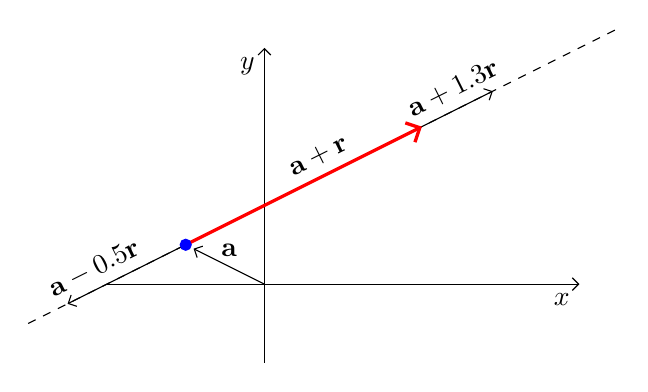
\begin{tikzpicture}[% styles used in image code
         > = Straight Barb, % defined in "arrows.meta
dot/.style = {circle, fill,
              minimum size=2mm, inner sep=0pt, outer sep=0pt,
              node contents={}},
box/.style = {draw, thin, minimum  width=2mm, minimum height=4mm,
              inner sep=0pt, outer sep=0pt,
              node contents={}, sloped},
my angle/.style args = {#1/#2}{draw,->,
                               angle radius=#1,
                               angle eccentricity=#2,
                               } % angle label position!
                        ]
	% coordinate axis
	\draw[->] (-2, 0) -- (4,0) node[below left] {$x$};
	\draw[->] ( 0,-1) -- (0,3) node[below left] {$y$};
	
	\draw[dashed,domain=-3:4.5,variable=\x] plot({\x},{0.5*\x+1});

	\coordinate (O) at (0,0);
	\coordinate (a) at (-1,0.5);
	\coordinate (r) at (3,1.5);
	
	\draw [->] (O) --($0.9*(a)$) node[pos=0.5,above] {$\mathbf{a}$};
	\draw [->] (a) --($(a)+1.3*(r)$) node[pos=0.9,above,rotate=26.5] {$\mathbf{a}+1.3\mathbf{r}$};
	\draw [->,red,very thick] (a) --($(a)+(r)$) node[pos=0.6,above,rotate=26.5,black] {$\mathbf{a}+\mathbf{r}$};
	\draw [->] (a) --($(a)-0.5*(r)$) node[pos=0.7,above,rotate=26.5] {$\mathbf{a}-0.5\mathbf{r}$};
	
	\filldraw [blue] (a) circle (2pt);
\end{tikzpicture}
\end{figure}
\noindent So this gives as the vector representation of a line.

\definition{Vector form of a straight line}{
The set of vectors in $\mathbb{R}^n$ of the form $\mathbf{v} = \mathbf{a} + t \mathbf{r}$ for a parameter $t\in\mathbb{R}$ represents a straight line through the space $\mathbb{R}^n$. That is,
\begin{align*}
\{(x,y) \, | \, \forall x\in\mathbb{R} \, \text{and} \, y=mx+b  \} = \{ \mathbf{a} + t \mathbf{r} \, | \, \forall t\in\mathbb{R} \}
\end{align*}
where $\mathbf{a}$ is an arbitrary pair $(x,mx+b)$ and $\mathbf{r}$ is a displacement vector between any two distinct pairs $(x_1,mx_1+b)$ and $(x_2,mx_2+b)$.
}


\section*{To do}
Unit vector

unit vector pointing in the direction of a given vector

Dot product as projection into another direction

\section{Summary of properties of Euclidean vectors}\label{sec:ch1_summary}

Let's collect a list of key properties of operations with tuples that will turn out not to be unique to tuples. The following are true for any tuples $\mathbf{a}$, $\mathbf{b}$ and $\mathbf{c} \in\mathbb{R}^n$ and any real numbers $k$ and $l\in\mathbb{R}$.

\begin{align*}
& \text{addition of tuples gives another tuple} && \quad \mathbf{a} + \mathbf{b} \in \mathbb{R}^n &\\
%
& \text{tuple addition is associative} && \quad (\mathbf{a} + \mathbf{b}) + \mathbf{c}  =\mathbf{a} + (\mathbf{b} + \mathbf{c}) &\\
%
& \text{the zero tuple is a tuple of zeros} && \quad \mathbf{a} + \mathbf{0} = \mathbf{0} + \mathbf{a} = \mathbf{a} &\\
%
& \text{the negative of a tuple is the additive inverse} && \quad \mathbf{a} + (-\mathbf{a}) = \mathbf{0} &\\
%
& \text{the order of tuple addition doesn't matter} && \quad \mathbf{a} + \mathbf{b} = \mathbf{b} + \mathbf{a} &\\
%
& \text{scalar multiplication of a tuple gives another tuple} && \quad k\mathbf{a} \in \mathbb{R}^n &\\
%
& \text{scalar multiplication distributes of tuple addition} && \quad k(\mathbf{a}+\mathbf{b})=k\mathbf{a}+k\mathbf{b} &\\
%
& \text{scalar addition distributes over tuples} && \quad (k+l)\mathbf{a}=k\mathbf{a}+l\mathbf{a} &\\
%
& \text{scalar multiplication order doesn't matter} && \quad k(l\mathbf{a})=(kl)\mathbf{a} &\\
%
& \text{scalar multiplication by 1 is an identity operation} && \quad 1\mathbf{a}=\mathbf{a} &
\end{align*}
\chapter{Matrix Algebra} \label{ch:matrixalgebra}

\section{Basic Definitions}

\definition{Matrix}{
A matrix is a collection of numbers from a field $\mathbb{F}$ (e.g. rational numbers) usually represented by a rectangular array. For example, an $m \times n$ (said m by n) matrix $A$ with coefficients $a_{ij}\in\mathbb{F}$  would be represented by an array with $m$ rows and $n$ columns:
\begin{align*}
A = 
\begin{pmatrix}
a_{11} & a_{12} & a_{13} & \cdots & a_{1j} & \cdots & a_{1m} \\
a_{21} & a_{22} & a_{23} & \cdots & a_{2j} & \cdots & a_{2m} \\
a_{31} & a_{32} & a_{33} & \cdots & a_{3j} & \cdots & a_{3m} \\
\vdots & \vdots & \vdots & \ddots & \vdots & \ddots & \vdots \\
a_{i1} & a_{12} & a_{13} & \cdots & a_{ij} & \cdots & a_{im} \\
\vdots & \vdots & \vdots & \ddots & \vdots & \ddots & \vdots \\
a_{n1} & a_{n2} & a_{n3} & \cdots & a_{nj} & \cdots & a_{nm}
\end{pmatrix}
=
\left( a_{ij} \right)_{\substack{ 1 \leq i \leq m \\ 1 \leq j \leq n }}.
\end{align*}
Sometimes it is convenient to refer to the coefficients in the array like so: $a_{ij} = \left(A\right)_{ij}$.
}

\definition{Set of all $m \times n$ matrices}{
We write the set of all $m \times n$ matrices with coefficients in $\mathbb{F}$ as
\begin{align*}
\mathcal{M}_{m,n}(\mathbb{F})
\end{align*}
}

\noindent It is sometimes useful in calculations to use the columns or rows of a matrix, and so we create the following notation.

\definition{Matrix columns and rows}{
For a matrix $A\in\mathcal{M}_{m,n}(\mathbb{F})$ we denote its j$^{th}$ column and i$^{th}$ row
\begin{align*}
A^{(j)} =
\begin{pmatrix}
 a_{1j} \\
 a_{2j} \\
 a_{3j} \\
 \vdots \\
 a_{ij} \\
 \vdots \\
 a_{mj}
\end{pmatrix},
\qquad
A_{(i)} =
\begin{pmatrix}
a_{i1} & a_{12} & a_{13} & \cdots & a_{ij} & \cdots & a_{in}
\end{pmatrix}
\end{align*}
}

\noindent For the rest of this course, unless otherwise noted, we will implicitly assume real matrices by writing $\mathcal{M}_{m,n}(\mathbb{R}) = \mathcal{M}_{m,n}$.

\definition{Transpose of a matrix}{
The transpose of an $m \times n$ matrix, $A$, is an $n \times m$ matrix, denoted $A^T$, with rows equal to the columns of $A$. That is, $\left(A^T\right)_{ij} = \left(A\right)_{ji}$ for all combinations of $i$ and $j$. 
}

\noindent For example
\begin{align*}
\begin{pmatrix}
1  & -2  \\
0  & -1  \\
-1 &  0
\end{pmatrix}^T
=
\begin{pmatrix}
 1  &  0 & -1\\
-2  & -1 &  0
\end{pmatrix}
\end{align*}


\definition{Diagonal matrix}{
A square matrix $A$ is said to be diagonal if all its non-diagonal elements are zero, e.g. $(A)_{ij}=0$ whenever $i \neq j$.
}

\definition{Symmetric matrix}{
A matrix $A$ is symmetric if it is equal to its transpose, $A = A^T$.
}


\noindent For example:
\begin{align*}
&\begin{pmatrix}
1.5 & 3 & \pi \\
3   & 2 & 2 \\
\pi & 2 & 1
\end{pmatrix}^T
=
\begin{pmatrix}
1.5 & 3 & \pi \\
3   & 2 & 2 \\
\pi & 2 & 1
\end{pmatrix}
\quad \text{symmetric} \\
%
&\begin{pmatrix}
1.5 & 1 & \pi \\
3   & 2 & 2 \\
7 & 2 & 1
\end{pmatrix}^T
=
\begin{pmatrix}
1.5 & 3 & 7 \\
1   & 2 & 2 \\
\pi & 2 & 1
\end{pmatrix}
\quad \text{not symmetric}
\end{align*}

\section{Matrix addition and scalar multiplication}


\definition{Matrix addition}{
Matrix addition is done coefficient by coefficient, that is, for two matrices $A$ and $B$ we define the i,j$^{th}$ coefficient of the addition as the addition of the i,j$^{th}$ coefficients of each matrix: 
\begin{align*}
\left(A+B\right)_{ij} = \left(A\right)_{ij}+\left(B\right)_{ij}.
\end{align*}
}

\noindent For example
\begin{align*}
\begin{pmatrix}
1 &  2 & -2 \\
3 & -1 & 0   
\end{pmatrix}
+
\begin{pmatrix}
0 & -1 & 3 \\
2 &  0 & 3   
\end{pmatrix}
=
\begin{pmatrix}
1+0 & 2-1 & -2+3 \\
3+2 & -1+0 & 0+3   
\end{pmatrix}
=
\begin{pmatrix}
1 &  1 & 1 \\
5 & -1 & 3   
\end{pmatrix}.
\end{align*}
This definition means that matrix addition is only well defined if the matrices have the same shape. It also implies that any two matrices $A,B \in \mathcal{M}_{m,n}$ add to give a third matrix $C \in \mathcal{M}_{m,n}$. That is, $\mathcal{M}_{m,n}$ is closed under addition with this definition.

\theorem{Matrix addition is associative}{ 
Given three matrices $A,B,C \in \mathcal{M}_{m,n}$:
\begin{align*}
A + (B + C) = (A + B) + C
\end{align*}
}

\begin{proof}
Let $D = B + C$, so that the definition of matrix addition gives us 
\begin{align*}
(D)_{ij}=(B)_{ij} + (C)_{ij}.
\end{align*}
Then $A + (B + C)= A + D$ has coefficients 
\begin{align*}
(A)_{ij} + (D)_{ij} = (A)_{ij} + ((B)_{ij} + (C)_{ij}).
\end{align*}
Addition in fields is associative, so
\begin{align*}
(A)_{ij} + ((B)_{ij} + (C)_{ij}) = ((A)_{ij} + (B)_{ij}) + (C)_{ij}
\end{align*}
These are exactly the coefficients of $(A+B)+C$.
\end{proof}

\theorem{Matrix addition is commutative}{ 
Given two matrices $A,B \in \mathcal{M}_{m,n}$:
\begin{align*}
A + B = B + A
\end{align*}
}



\definition{Scalar multiplication}{
Given a number $k\in\mathbb{R}$ (called a scalar) and a matrix $A \in \mathcal{M}_{m,n}$, we define matrix scalar multiplication, $kA$, to be a matrix $B \in \mathcal{M}_{m,n}$ with coefficients given by:
\begin{align*}
b_{ij} = ka_{ij},
\end{align*}
that is, we multiply \textit{every coefficient} by the scalar.
} 

\noindent For example:
\begin{gather*}
k
\begin{pmatrix}
 1 & 3 \\
 7 & 2 
\end{pmatrix}
=
\begin{pmatrix}
 k & 3k \\
 7k & 2k 
\end{pmatrix}
%%%%%%%%
%%%%%%%%
\\
%%%%%%%%
%%%%%%%%
\frac{1}{2}
\begin{pmatrix}
 2 & 2 \\
 1 & 1 \\
 0 & 3 
\end{pmatrix}
=
\begin{pmatrix}
 1 & 1 \\
 1/2 & 1/2 \\
 0 & 3/2 
\end{pmatrix}
\end{gather*}

\theorem{Scalar multiplication is distributive}{
For any scalars $\alpha,\beta \in \mathbb{R}$ and matrices $A,B \in \mathcal{M}_{n,m}$, scalar multiplication on matrices is both distributive over matrix addition:
\begin{align*}
\alpha(A + B) = \alpha A + \alpha B
\end{align*}
and distributive over scalar addition
\begin{align*}
(\alpha + \beta)A = \alpha A + \beta A.
\end{align*}
}

\theorem{Scalar multiplication is associative}{
For any scalars $\alpha,\beta \in \mathbb{R}$ and matrix $A$, scalar multiplication is associative in the following sense:
\begin{align*}
\alpha(\beta A) = (\alpha \beta ) A.
\end{align*}
}

The concept of zero is fundamentally that when we add zero to something we get back the same thing. For matrices then we want, for a matrix $A$, that $A + M_0 = A$. First this means this zero object must be a matrix of the same shape as $A$. Looking at coefficients, we have
\begin{align*}
(A + M_0)_{ij} = (A)_{ij} + (M_0)_{ij} = A_{ij} \implies (M_0)_{ij} = 0
\end{align*}
This gives the following definition.

\definition{Zero matrix}{
The zero matrix of any shape is a matrix $M_0 \in\mathcal{M}_{m,n}$ consisting entirely of zeros as coefficients.
} 
Note that this means there is no unique zero matrix, but rather a zero matrix for every possible matrix shape.

\example{Zero matrices}{
\begin{align*}
\begin{pmatrix}
0 & 0 & 0 & 0 \\
0 & 0 & 0 & 0 
\end{pmatrix}
\quad\quad
\begin{pmatrix}
0 & 0 \\
0 & 0 \\
0 & 0 
\end{pmatrix}
\end{align*}
}

With this zero matrix we can find the additive inverse of a matrix, $A\in\mathcal{M}_{m,n}$, by considering the defining relation $A+B=M_0$, where $B$ is the additive inverse of $A$. This means
\begin{align*}
(A+B)_{ij} = (A)_{ij}+(B)_{ij} = 0 \implies (B)_{ij} = - (A)_{ij} = (-A)_{ij}
\end{align*}

\definition{Additive inverse}{
Given a matrix $A\in\mathcal{M}_{ij}$, its additive inverse is the same matrix multiplied by the scalar $-1$. We denote the additive inverse of $A$ as $-A$.
} 

\example{Additive inverses}{
\begin{gather*}
A=
\begin{pmatrix}
2 & 0 & -1 \\
0 & 1 &  3 
\end{pmatrix}
\quad\implies\quad
-A=
\begin{pmatrix}
 -2 &  0 &  1 \\
  0 & -1 & -3 
\end{pmatrix}
\\
B=
\begin{pmatrix}
  3 & -1 \\
\pi &  0 
\end{pmatrix}
\quad\implies\quad
-B=
\begin{pmatrix}
  -3 &  1 \\
-\pi &  0 
\end{pmatrix}
\end{gather*}
}





\subsection*{Summary of properties of matrix addition and scalar multiplication}

Let's collect a list of key properties of operations with matrices that are shared with tuples. The following are true for any matrices $A,B,C\in\mathcal{M}_{m,n}$ and any real numbers $k$ and $l\in\mathbb{R}$.

\begin{align*}
& \text{addition of matrices gives another matrix} && \quad A + B \in\mathcal{M}_{m,n} &\\
%
& \text{matrix addition is associative} && \quad (A + B) + C = A + (B + C) &\\
%
& \text{the zero matrix is a matrix of zeros} && \quad A + M_0 = M_0 + A = A &\\
%
& \text{the negative of a matrix is the additive inverse} && \quad A + (-A) = M_0 &\\
%
& \text{the order of matrix addition doesn't matter} && \quad A + B = B + A &\\
%
& \text{scalar multiplication of a matrix gives another matrix} && \quad kA\in\mathcal{M}_{m,n} &\\
%
& \text{scalar multiplication distributes of matrix addition} && \quad k(A+B)=kA+kB &\\
%
& \text{scalar addition distributes over matrix} && \quad (k+l)A=kA+lA &\\
%
& \text{scalar multiplication order doesn't matter} && \quad k(lA)=(kl)A &\\
%
& \text{scalar multiplication by 1 is an identity operation} && \quad 1A=A &
\end{align*}


\section{Multiplication of matrices by columns}

When restricting ourselves to simple addition of matrices or scalar multiplication we see that matrices and tuples have the same rules. In fact we could simply think of tuples as $2\times 1$ or $1\times 2$ matrices. Here we will introduce a new type of multiplication, that of matrices by matrices. This is not the same as the dot product.

\definition{Multiplication of a matrix by a column}{
Consider a matrix $A \in \mathcal{M}_{m,n}$ and a column $X \in \mathcal{M}_{n,1}$. We define the product $AX$ to result in the column $Y\in\mathcal{M}_{m,1}$ with coefficients
\begin{align*}
(Y)_i = a_{i1}x_1 + a_{i2}x_2 + \cdots + a_{im}x_m = \sum_{k=1}^m a_{ik} x_k 
\end{align*}
Visually
\begin{align*}
\begin{pmatrix}
y_{1} \\
y_{2} \\
\vdots \\
y_{n} 
\end{pmatrix}
%%%
%%%
%%%
&=
%%%
\begin{pmatrix}
a_{11} & a_{12} & \cdots & a_{1m} \\
a_{21} & a_{22} & \cdots & a_{2m} \\
\vdots & \vdots & \ddots & \vdots \\
a_{n1} & a_{n2} & \cdots & a_{nm}
\end{pmatrix}
\begin{pmatrix}
x_{1} \\
x_{2} \\
\vdots \\
x_{m} 
\end{pmatrix}
%%%
%%%
%%%
=
%%%
x_{1}
\begin{pmatrix}
a_{11} \\
a_{21} \\
\vdots \\
a_{n1} 
\end{pmatrix}
+
x_{2}
\begin{pmatrix}
a_{12} \\
a_{22} \\
\vdots \\
a_{n2} 
\end{pmatrix}
+ \cdots +
x_m
\begin{pmatrix}
a_{1m} \\
a_{2m} \\
\vdots \\
a_{nm} 
\end{pmatrix}
\\ \\
%%%
%%%
%%%
&\implies Y = x_{1}A^{(1)} + x_{2}A^{(2)} + \cdots + x_{m}A^{(m)}
\end{align*}
}

\noindent Notice that in this definition, to be able to multiply a matrix by a column the matrix must have the same number of columns as the elements of the column. Additionally, the answer will be a column of the same shape as the columns of the matrix, \textit{not the column that is multipled by the matrix}.

\noindent Note also that not only is multiplication of matrices by columns not commutative, $AX \neq XA$, but that the latter is not even defined. We cannot multiply a column by a matrix left to right.

\example{Matrix multiplication by columns}{
\begin{align*}
& \begin{pmatrix}
      1 &  2 & 4  \\
      3 & -1 & 0
\end{pmatrix}
\begin{pmatrix}
      3 \\
     -1 \\
      2
\end{pmatrix}
=
3\begin{pmatrix}
1 \\
3
\end{pmatrix}
-
1\begin{pmatrix}
2 \\
-1
\end{pmatrix}
+
2\begin{pmatrix}
4 \\
0
\end{pmatrix}
=
\begin{pmatrix}
 9 \\
 10
\end{pmatrix} \\
%%%%%
%%%%%
%%%%%
& \begin{pmatrix}
      1 &  3  \\
      2 & -1 \\
      0 &  4       
\end{pmatrix}
\begin{pmatrix}
      3 \\
      2
\end{pmatrix}
=
3\begin{pmatrix}
      1 \\
      2 \\
      0  
\end{pmatrix}
+
2\begin{pmatrix}
      3  \\
     -1 \\
      4       
\end{pmatrix}
=
\begin{pmatrix}
      9 \\
      4 \\
      8       
\end{pmatrix}
\end{align*}
}

\noindent There is another method of remembering how to do this matrix multiplication. It comes from recognising the dot product in the calculation of the coefficients. Recall for $AX=Y$ we have
\begin{align*}
(Y)_i = a_{i1}x_1 + a_{i2}x_2 + \cdots + a_{im}x_m = \left(a_{i1},\,a_{i2}, \dots, a_{im}  \right) \cdot \left(x_{1},\,x_{2}, \dots, x_{m}  \right)
\end{align*}
where we have the i$^{th}$ row of $A$ and the column $X$ interpreted as tuples. We make a small notational modification, denoting with bold font, e.g. $\mathbf{A}_{(i)}$ or $\mathbf{X}$, that we interpret a column as a tuple. Then we can write $(Y)_i = \mathbf{A}_{(i)} \cdot \mathbf{X}$. Just be careful to note that we aren't right now using the objects $A_{(i)}$ and $X$, but rather their tuple versions.



\example{Matrix multiplication by columns with dot product}{
Let $A=\begin{pmatrix}
      1 &  2 & 1  \\
      3 &  0 & 0  \\
      2 &  1 & 1
\end{pmatrix}$ and $X=\begin{pmatrix} 1 \\ 2 \\ 3 \end{pmatrix}$. Then we have
\begin{align*}
& AX = \begin{pmatrix}
      1 &  2 & 1  \\
      3 &  0 & 0  \\
      2 &  1 & 1
\end{pmatrix}
\begin{pmatrix} 1 \\ 2 \\ 3 \end{pmatrix}
=
\begin{pmatrix}
 \mathbf{A}_{(1)} \cdot \mathbf{X} \\
 \mathbf{A}_{(2)} \cdot \mathbf{X} \\
 \mathbf{A}_{(3)} \cdot \mathbf{X}
\end{pmatrix}
=
\begin{pmatrix}
 (1, 2, 1) \cdot (1, 2, 3) \\
 (3, 0, 0) \cdot (1, 2, 3) \\
 (2, 1, 1) \cdot (1, 2, 3)
\end{pmatrix}
=
\begin{pmatrix}
 1 \times 1 + 2 \times 2 + 1 \times 3 \\
 3 \times 1 + 0 \times 2 + 0 \times 3 \\
 2 \times 1 + 1 \times 2 + 1 \times 3
\end{pmatrix}
=
\begin{pmatrix}
 8 \\
 3 \\
 7
\end{pmatrix}
\end{align*}
}

\section{Euclidean transformation matrices}
\subsection*{Rotation matrices}

\noindent One notable usage of multiplication of matrices by columns is the representation of operation of rotating Euclidean vectors. Consider an arbitrary Euclidean vector $\mathbf{v}\in\mathbb{R}^2$ with decomposition $\mathbf{v} = (x ,y)$. Say we want to rotate this vector anti-clockwise an angle $\theta$, with the result a new vector $\mathbf{w} = (x' ,y')$, as pictured below.

\begin{figure}[H]
\centering
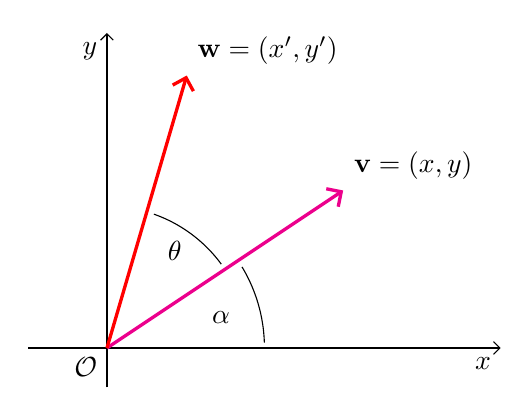
\begin{tikzpicture}[% styles used in image code
         > = Straight Barb, % defined in "arrows.meta
dot/.style = {circle, fill,
              minimum size=2mm, inner sep=0pt, outer sep=0pt,
              node contents={}},
box/.style = {draw, thin, minimum  width=2mm, minimum height=4mm,
              inner sep=0pt, outer sep=0pt,
              node contents={}, sloped},
my angle/.style args = {#1/#2}{draw,->,
                               angle radius=#1,
                               angle eccentricity=#2,
                               } % angle label position!
                        ]
	% coordinate axis
	\draw[->] (-1, 0)   -- (5,0) node[below left] {$x$};
	\draw[->] ( 0,-0.5) -- (0,4) node[below left] {$y$};

	\coordinate (O) at (0,0);
	\coordinate (v1) at (3,2);
	\coordinate (v2) at (1.013,3.460);
	
	\draw (O) node[below left] {$\mathcal{O}$};
	\draw [->,magenta,very thick] (O) --(v1) node[above right,black] {$\mathbf{v}=(x,y)$};
	\draw [->,red,very thick] (O) --(v2) node[above right,black] {$\mathbf{w}=(x',y')$};
	
	\begin{scope}
	\path[clip] (O) -- (3,0.1) -- ($(v1)+(0,-0.2)$);
	\draw[black] (O) circle (20mm);
	\node at ($(O)+(15:15mm)$) {$\alpha$};
	\end{scope}
	
	\begin{scope}
	\path[clip] (O) -- ($(v1)+(0,0.2)$) -- ($(v2)+(0.2,0)$);
	\draw[black] (O) circle (18mm);
	\node at ($(O)+(55:15mm)$) {$\theta$};
	\end{scope}
\end{tikzpicture} \caption*{Rotation of Euclidean vectors.}
\end{figure}

\noindent The rotated vector has a decomposition with its norm and angle as
\begin{align*}
x' &= \|\mathbf{w}\| \cos(\alpha+\theta)\\
y' &= \|\mathbf{w}\| \sin(\alpha+\theta)
\end{align*}
Rotation doesn't change the norm of a vector, so $\|\mathbf{w}\| = \|\mathbf{v}\| = \sqrt{x^2+y^2}$. Then, using the angle sum trigonometry identities we have
\begin{align*}
&\begin{array}{l}
x' = \sqrt{x^2+y^2} \left( \cos\alpha\cos\theta-\sin\alpha\sin\theta \right)\\
y' = \sqrt{x^2+y^2} \left( \sin\alpha\cos\theta + \cos\alpha\sin\theta \right)
\end{array} \\ \\
\implies
& \begin{array}{l}
x' = \sqrt{x^2+y^2} \left( \dfrac{x}{\sqrt{x^2+y^2}}\cos\theta-\dfrac{y}{\sqrt{x^2+y^2}}\sin\theta \right)\\
y' = \sqrt{x^2+y^2} \left( \dfrac{y}{\sqrt{x^2+y^2}}\cos\theta + \dfrac{x}{\sqrt{x^2+y^2}}\sin\theta \right)
\end{array} \\ \\
\implies
& \begin{array}{l}
x' = x\cos\theta-y\sin\theta \\
y' = y\cos\theta + x\sin\theta 
\end{array}
\end{align*}
We can represent the rotated vector as the column
\begin{align*}
\begin{pmatrix} x' \\ y' \end{pmatrix}
=
\begin{pmatrix} 
x\cos\theta - y\sin\theta \\ 
x\sin\theta + y\cos\theta 
\end{pmatrix}
=
\begin{pmatrix} 
x\cos\theta \\ 
x\sin\theta
\end{pmatrix}
+
\begin{pmatrix} 
- y\sin\theta \\ 
y\cos\theta 
\end{pmatrix}
=
x
\begin{pmatrix} 
\cos\theta \\ 
\sin\theta
\end{pmatrix}
+
y
\begin{pmatrix} 
- \sin\theta \\ 
\cos\theta 
\end{pmatrix}
\end{align*}
This last expression is how we've defined a matrix multiplied by a column! So we have
\begin{gather*}
\begin{pmatrix} x' \\ y' \end{pmatrix}
=
\begin{pmatrix} 
\cos\theta & -\sin\theta \\ 
\sin\theta &  \cos\theta  
\end{pmatrix}
\begin{pmatrix} x \\ y \end{pmatrix}
\end{gather*}
which gives us the definition of the general rotation matrix:

\definition{Rotation matrix - arbtirary angle anti-clockwise}{
By using a column $X\in\mathcal{M}_{2,1}$ to represent a Euclidean vector, the following matrix allows the operation of rotataion, anti-clockwise, of $X$ by an angle $\theta$:
\begin{align*}
R_\theta =
\begin{pmatrix} 
\cos\theta & -\sin\theta \\ 
\sin\theta &  \cos\theta  
\end{pmatrix}
\end{align*}
where the rotated vector is represented by a column $X'\in\mathcal{M}_{2,1}$ obtained by matrix multiplication $X' = R_\theta X$.
}

\subsection*{Reflection matrices}

\subsection*{Compression and dilation matrices}

\subsection*{Skew matrices}

\subsection*{Summary of Euclidean transformation matrices}

\begin{table}[H]
\begin{center}
\begin{tabular}{l|l}
Transformation & Matrix \\ \hline\hline \\[-7pt]
Rotation by 45 degrees & $R_{\theta=\pi/4} = \dfrac{1}{\sqrt{2}}\begin{pmatrix} 1 & -1 \\ 1 & 1 \end{pmatrix}$ \\[10pt] \hline  \\[-7pt]
Rotation by 90 degrees & $R_{\theta=\pi/2} = \begin{pmatrix} 0 & -1 \\ 1 & 0 \end{pmatrix}$ \\[10pt] \hline \\[-7pt]
Rotation by $\theta$ degrees & $R_{\theta} = \begin{pmatrix} \cos\theta & -\sin\theta \\ \sin\theta & \cos\theta \end{pmatrix}$ \\[10pt] \hline \\[-7pt]
Reflection across $x$-axis & $R_{x} = \begin{pmatrix} 1 & 0 \\ 0 & -1 \end{pmatrix}$ \\ [10pt] \hline \\[-7pt]
Reflection across $y$-axis & $R_{y} = \begin{pmatrix} -1 & 0 \\ 0 & 1 \end{pmatrix}$ \\ [10pt] \hline \\[-7pt]
Reflection across $y=x$ line & $R_{y=x} = \begin{pmatrix} 0 & 1 \\ 1 & 0 \end{pmatrix}$ \\ [10pt] \hline \\[-7pt]
Reflection across $y=-x$ line & $R_{y=-x} = \begin{pmatrix} 0 & -1 \\ -1 & 0 \end{pmatrix}$ \\[10pt] \hline \\[-7pt]
Reflection across origin & $R_{\mathcal{O}} = \begin{pmatrix} -1 & 0 \\ 0 & -1 \end{pmatrix}$ \\[10pt] \hline \\[-7pt]
Dilation & $D = \begin{pmatrix} k & 0 \\ 0 & k \end{pmatrix}, \quad k>1$ \\[10pt] \hline \\[-7pt]
Compression & $D = \begin{pmatrix} k & 0 \\ 0 & k \end{pmatrix}, \quad 0\leq k<1$ \\[10pt] \hline \\[-7pt]
Skew in the $x$ direction & $S_{x,k} = \begin{pmatrix} k & 0 \\ 0 & 1 \end{pmatrix}$ \\[10pt] \hline \\[-7pt]
Skew in the $y$ direction & $S_{y,k} = \begin{pmatrix} 1 & 0 \\ 0 & k \end{pmatrix}$
\end{tabular}
\end{center}
\end{table}

\section{Multiplication of matrices by matrices}

We will start with the definition of matrix multiplication before justifying some of its properties.

\definition{Multiplication of two matrices}{
Consider two matrices $A \in \mathcal{M}_{n,m}$ and $B \in \mathcal{M}_{m,q}$. We define the product $AB$ to be the matrix $C\in\mathcal{M}_{n,q}$ with coefficients
\begin{gather*}
c_{ij} = a_{i1}b_{1j} + a_{i2}b_{2j} + \cdots + a_{im}b_{mj} = \sum_{k=1}^m a_{ik} b_{kj} \\
%%%
%%%
%%%
\implies
\begin{pmatrix}
a_{11} & a_{12} & \cdots & a_{1m} \\
a_{21} & a_{22} & \cdots & a_{2m} \\
\vdots & \vdots & \ddots & \vdots \\
a_{n1} & a_{n2} & \cdots & a_{nm}
\end{pmatrix}
\begin{pmatrix}
b_{11} & b_{12} & \cdots & b_{1q} \\
b_{21} & b_{22} & \cdots & b_{2q} \\
\vdots & \vdots & \ddots & \vdots \\
b_{m1} & b_{m2} & \cdots & b_{mq}
\end{pmatrix} \\
%%%
%%%
%%%
=
\left(
b_{11}
\underbrace{
\begin{pmatrix}
a_{11} \\
a_{21} \\
\vdots \\
a_{n1} 
\end{pmatrix}
+ \cdots +
b_{m1}
\begin{pmatrix}
a_{1m} \\
a_{2m} \\
\vdots \\
a_{nm} 
\end{pmatrix}
}_{\text{\large first column}}
%%
\quad \cdots \quad 
%%
b_{1q}
\underbrace{
\begin{pmatrix}
a_{11} \\
a_{21} \\
\vdots \\
a_{n1} 
\end{pmatrix}
+ \cdots +
b_{mq}
\begin{pmatrix}
a_{1m} \\
a_{2m} \\
\vdots \\
a_{nm} 
\end{pmatrix}
}_{\text{\large n$^{th}$ column}}
\right)
\end{gather*}
Additionally, for the product
\begin{align*}
\underbrace{A}_{(\colorbox{Mahogany!20}{n},\colorbox{airforceblue!20}{m})} \underbrace{B}_{(\colorbox{airforceblue!20}{m},\colorbox{Mahogany!20}{q})}
\end{align*}
we will call the indices for the columns of $A$ and rows of $B$ the \textit{inner indices} (blue), whereas the indices for the rows of $A$ and columns of $B$ will be called the \textit{outer indices} (red).
}

\example{Matrix multiplication}{
\begin{align*}
\begin{pmatrix}
      1 &  2 & 4  \\
      3 & -1 & 0  \\
\end{pmatrix}
\begin{pmatrix}
      2 &  5  \\
      1 &  3  \\
     -1 & -4  \\
\end{pmatrix}
=
\left(
\overbrace{
2\begin{pmatrix}
1 \\
3
\end{pmatrix}
+
1\begin{pmatrix}
2 \\
-1
\end{pmatrix}
-1\begin{pmatrix}
4 \\
0
\end{pmatrix}
}^{\text{\large first column}}
%%%
\quad
%%%
\overbrace{
5\begin{pmatrix}
1 \\
3
\end{pmatrix}
+
3\begin{pmatrix}
2 \\
-1
\end{pmatrix}
-4\begin{pmatrix}
4 \\
0
\end{pmatrix}
}^{\text{\large second column}}
\right)
=
\begin{pmatrix}
 0 & -5 \\
 5 & 12
\end{pmatrix}
\end{align*}
}

\noindent It should be clear that the j$^{th}$ column of the result is like we just did matrix multiplication of $A$ by the j$^{th}$ column of $B$. Otherwise put, the i,j$^{th}$ element of $AB$ comes from the dot product of the i$^{th}$ row of $A$ by the j$^{th}$ column of $B$: $c_{ij}=(a_{i1}, a_{i2}, \dots , a_{im})\cdot(b_{1j},b_{2j},\dots,b_{mj})=\mathbf{A_{(i)}}\cdot\mathbf{B^{(j)}}$. Visually:
\begin{align*}
&
\begin{pmatrix}
a_{11} & a_{12} & \cdots & a_{1m} \\
a_{21} & a_{22} & \cdots & a_{2m} \\
\vdots & \vdots & \ddots & \vdots \\
a_{n1} & a_{n2} & \cdots & a_{nm}
\end{pmatrix}
\begin{pmatrix}
b_{11} & b_{12} & \cdots & b_{1q} \\
b_{21} & b_{22} & \cdots & b_{2q} \\
\vdots & \vdots & \ddots & \vdots \\
b_{m1} & b_{m2} & \cdots & b_{mq}
\end{pmatrix} \\
&=
\begin{pmatrix}
\mathbf{A}_{(1)}\cdot\mathbf{B}^{(1)} & \mathbf{A}_{(1)}\cdot\mathbf{B}^{(2)} & \cdots & \mathbf{A}_{(1)}\cdot\mathbf{B}^{(m)} \\
\mathbf{A}_{(2)}\cdot\mathbf{B}^{(1)} & \mathbf{A}_{(2)}\cdot\mathbf{B}^{(2)} & \cdots & \mathbf{A}_{(2)}\cdot\mathbf{B}^{(m)} \\
\vdots & \vdots & \ddots & \vdots \\
\mathbf{A}_{(n)}\cdot\mathbf{B}^{(1)} & \mathbf{A}_{n}\cdot\mathbf{B}^{(2)} & \cdots & \mathbf{A}_{(n)}\cdot\mathbf{B}^{(m)}
\end{pmatrix}
\end{align*}



\example{Matrix multiplication with dot products}{
\begin{align*}
\begin{pmatrix}
      3 &  0 \\
     -1 &  2
\end{pmatrix}
\begin{pmatrix}
      1 &  2 & -4  \\
      1 & -3 &  1
\end{pmatrix}
&=
\begin{pmatrix}
  \mathbf{A}_{(1)}\cdot\mathbf{B}^{(1)} & \mathbf{A}_{(1)}\cdot\mathbf{B}^{(2)}  & \mathbf{A}_{(1)}\cdot\mathbf{B}^{(3)}  \\
  \mathbf{A}_{(2)}\cdot\mathbf{B}^{(1)}  & \mathbf{A}_{(2)}\cdot\mathbf{B}^{(2)} &  \mathbf{A}_{(2)}\cdot\mathbf{B}^{(3)}
\end{pmatrix}
%%%%
%%%%
%%%%
\\
&=
\begin{pmatrix}
  (3,0)\cdot(1,1) & (3,0)\cdot(2,-3)  & (3,0)\cdot(-4,1)  \\
  (-1,2)\cdot(1,1) & (-1,2)\cdot(2,-3)  & (-1,2)\cdot(-4,1)
\end{pmatrix} 
\\
&=
\begin{pmatrix}
  3 &  6  & -12  \\
  1 & -8  &   6
\end{pmatrix}
\end{align*}
}

Let's now try to understand why the shapes must be what they are. Suppose we have two matrices $A$ and $B$. We would like to define the matrix multiplication $AB=C$ so that the following associative law holds:
\begin{align*}
CX = (AB)X = A(BX)
\end{align*}
for a column $X$ of an appropriate size. 

Let's start with $B$ as the matrix with known size $m \times n$. This forces the size of $X$ \textit{given how we defined multiplication of a matrix by a column}: $X$ must have the same number of elements as \textit{columns} of $B$. So $X\in\mathcal{M}_{n,1}$ and the multiplication $BX$ gives a new column $X'$ with known shape: 
\begin{align*}
\underbrace{B}_{(m,n)} \underbrace{X}_{(n,1)} = \underbrace{X'}_{(m,1)}
\end{align*}
So $A(BX)$ becomes $AX'$, another multiplication of a matrix by a column. So $A$ must have the same number of columns as the elements of the column it multiplies: $A\in\mathcal{M}_{q,n}$ for some $q$. The multiplication $AX'$ gives a new column $X''$ with known shape: 
\begin{align*}
\underbrace{A}_{(q,n)} \underbrace{X'}_{(n,1)} = \underbrace{X''}_{(q,1)}
\end{align*}
Finally we have $CX = X''$. This forces the shape of $C$, the product of $A$ and $B$. $C$ must have the same number of columns as elements of $X$, $n$. The column $X''$ must have the same number of elements, $q$, as \textit{rows} of $C$. So we have $C\in\mathcal{M}_{q,n}$. Notice that this means the shape of the product $A$ and $B$ comes from the outer indices of their shapes:
\begin{align*}
\underbrace{A}_{(\colorbox{Mahogany!20}{n},\colorbox{airforceblue!20}{m})} \underbrace{B}_{(\colorbox{airforceblue!20}{m},\colorbox{ForestGreen!30}{q})} = \underbrace{C}_{(\colorbox{Mahogany!20}{n},\colorbox{ForestGreen!30}{q})}
\end{align*}
The inner indices must be the same, $m$ in this case, and doesn't appear in the answer.




\example{Multiplication of rotation matrices}{
Let $R_\theta$ and $R_\phi$ be anti-clockwise rotation matrices for angles $\theta$ and $\phi$. That is
\begin{align*}
R_\theta
=
\begin{pmatrix} \cos\theta & -\sin\theta \\ \sin\theta & \cos\theta \end{pmatrix}
\quad \text{and} \quad
R_\alpha
=
\begin{pmatrix} \cos\phi & -\sin\phi \\ \sin\phi & \cos\phi \end{pmatrix}
\end{align*}
When we multiply these matrices we get
\begin{align*}
R_\theta R_\alpha
&=
\begin{pmatrix} \cos\theta & -\sin\theta \\ \sin\theta & \cos\theta \end{pmatrix}
\begin{pmatrix} \cos\phi & -\sin\phi \\ \sin\phi & \cos\phi \end{pmatrix} \\
&=
\begin{pmatrix}
\cos\theta\cos\phi - \sin\theta\sin\phi & -\cos\theta\sin\phi -\sin\theta\cos\phi \\
\sin\theta\cos\phi + \cos\theta\sin\phi & -\sin\theta\sin\phi +\cos\theta\cos\phi
\end{pmatrix} \\
&=
\begin{pmatrix}
\cos(\theta+\phi) & -\sin(\theta+\phi) \\
\sin(\theta+\phi) & \cos(\theta+\phi)
\end{pmatrix}
\end{align*}
This result is just an anti-clockwise rotation matrix for angle $\theta+\phi$. This should make sense. Rotating a vector by $\theta$, and then rotating the resulting vector by $\phi$ is the same as doing it in one go by the addition of these angles.
}

\theorem{Square matrix multiplication and commutativity}{
For any two matrices $A$ and $B$, if the products $AB$ and $BA$ are well defined then both products result in square matrices. If the products give the same result, $AB=BA$, then both $A$ and $B$ must also be square matrices of the same shape.
}
\begin{proof}
Let $A\in\mathcal{M}_{m,n}$ and $B\in\mathcal{M}_{p,q}$. Then for $AB$ to be well defined, recall that the inner indices must be equal: the number of columns of $A$ must match the number of rows of $B$, so $n=p$. Similarly for $BA$ to be well defined, the number of columns of $B$ must match the number of rows of $A$, so $q=m$. Hence $B\in\mathcal{M}_{n,m}$ and therefore
\begin{itemize}
\item $AB \in\mathcal{M}_{m,m}$, and
\item $BA \in\mathcal{M}_{n,n}$.
\end{itemize}
Now if we have that $AB=BA$ we must have that $m=n$. Hence
\begin{itemize}
\item $A \in\mathcal{M}_{m,n}=\mathcal{M}_{m,m}$, and
\item $B \in\mathcal{M}_{p,q}=\mathcal{M}_{n,m}=\mathcal{M}_{m,m}$.
\end{itemize}

\end{proof}

\noindent Now that multiplication of matrices is well defined, we can introduce the notion of the multiplicative identity, the parallel of the number 1 for matrices. That is, the identity matrix $I$ should multiply by any matrix, say $A$, and return the same: $IA=A$. Suppose $A\in\mathcal{M}_{m,n}$ and $I\in\mathcal{M}_{p,q}$, so we have
\begin{align*}
\underbrace{I}_{(p,q)} \underbrace{A}_{(m,n)} = \underbrace{A}_{(m,n)}.
\end{align*}
Then to satisfy the shapes condition we must have that the inner indices match, so $q=m$, and outer indices give the resulting shape, so $p=m$. So $I$ must be a square matrix $I\in\mathcal{M}_{m,m}$ where the size matches the number of rows of $A$. Now we can look at each element in the product
\begin{align*}
(IA)_{ij} &= \mathbf{I}_{(i)}\cdot\mathbf{A}^{(j)} \\
&= (I)_{i1}a_{1j} + (I)_{i2}a_{2j} + \cdots + (I)_{ii}a_{ij} + \cdots + (I)_{im}a_{mj}.
\end{align*}
This must equal $a_{ij}$ to satisfy $IA=A$ and so $(I)_{ik}=0$ for all the $k$ except $k=i$ where $(I)_{ii}=1$. So we have the following definition.

\definition{Identity matrix}{
The $n$-dimensional identity matrix $I$ is a square matrix of size $n\times n$ with 1s along the diagonal and 0s elsewhere, that is, 
\begin{align*}
(I)_{ij}
=
\begin{cases}
1 & \text{whenever } \, i=j, \\
0 & \text{whenever } \, i \neq j.
\end{cases}
\end{align*}
}

\example{Identity matrices}{
\begin{align*}
I_2 =
\begin{pmatrix}
1 & 0 \\
0 & 1
\end{pmatrix}
\quad\quad
I_3 =
\begin{pmatrix}
1 & 0 & 0 \\
0 & 1 & 0 \\
0 & 0 & 1
\end{pmatrix}
\end{align*}
}

We have defined above, in fact, the \textit{left} identity matrix because the defining relation was multiplication on the left $IA=A$. If we have $AI=A$ then by the previous reasoning we find $I$ must be a square matrix with size matching the columns of $A$ instead. It's only in the case that $A$ itself is a square matrix that we can have a two-sided identity matrix satisfying $IA=AI=A$.

\example{Matrix multiplication giving the zero matrix}{
Curiously, we can have two non-zero matrices multiply to give a zero matrix:
\begin{gather*}
\begin{pmatrix}
1 & 2 \\
0 & 0
\end{pmatrix}
\begin{pmatrix}
0 & 3 \\
0 & 2
\end{pmatrix}
=
\begin{pmatrix}
0 & 0 \\
0 & 0
\end{pmatrix}
\\
\begin{pmatrix}
1 & 2 & 0 \\
1 & 0 & -1
\end{pmatrix}
\begin{pmatrix}
0 &  2 \\
0 & -1 \\
0 &  2
\end{pmatrix}
=
\begin{pmatrix}
0 & 0 \\
0 & 0
\end{pmatrix}
\end{gather*}
}


Just like the zero matrix gives us the idea of the additive inverse, the identity matrix gives the idea of the \textit{multiplicative} inverse. However, though every matrix has an additive inverse, not every matrix will have a multiplicative inverse. The following gives the defining relation of invertible matrices.

\definition{Invertible matrix}{
A matrix $A$ is invertible if and only if there exists a matrix $B$ such that
\begin{align*}
A B = BA = I
\end{align*}
This matrix $B$ is called the inverse of $A$ and is denoted $A^{-1}$. As we have commutative matrices, $AB=BA$, recall that this can only happen if $A$ is square. So, only square matrices can have inverses.
}

\example{Invertible matrix}{
Let $A=\begin{pmatrix} 1 & 2 \\ 0 & -1 \end{pmatrix}$. Given that
\begin{align*}
\begin{pmatrix} 1 & 2 \\ 3 & -1 \end{pmatrix}
\begin{pmatrix} 1/7 & 2/7 \\ 3/7 & -1/7 \end{pmatrix}
=
\begin{pmatrix} 1 & 0 \\ 0 & 1 \end{pmatrix},
\end{align*}
then we have $A^{-1}=\begin{pmatrix} 1/7 & 2/7 \\ 3/7 & -1/7 \end{pmatrix}$.
}

\noindent Before we develop techniques for finding inverses of matrices, we will introduce a function that allows us to determine \textit{whether} a given square matrix is invertible or not. This function is called the determinant. 

\section{Determinants of matrices}

The idea of the determinant of a matrix is to assign a single number to any square matrix which can be used to determine if that matrix is invertible or not. It will turn out that the determinant of a matrix will break down into determinants of smaller matrices. So we start with determinants of 1 by 1 matrices.

Suppose we have a general 1 by 1 matrix $A = \begin{pmatrix} a \end{pmatrix}$. It shouldn't be too difficult to see that the inverse matrix must be $A^{-1} = \begin{pmatrix} 1/a \end{pmatrix}$ because the multiplication $\begin{pmatrix} a \end{pmatrix}\begin{pmatrix} 1/a \end{pmatrix} = \begin{pmatrix} 1 \end{pmatrix}$, the identity matrix. Since $1/a$ is well defined only if $a\neq 0$, the value of $a$ itself satisfies this idea ``if this value is non-zero, the matrix is invertible''. So we have justified the following.

\definition{Determinant of a 1 by 1 matrix}{
The determinant of any 1 by 1 matrix is given by its only coefficient:

\begin{align*}
\det \left( \begin{pmatrix} a \end{pmatrix}\right)  = a
\end{align*}
}

Now, to define the determinant of any matrix, as stated before there is an iterative process where the determinant of an $n\times n$ matrix is equal to a certain combination of determinants of $n-1 \times n-1$ matrices. So we first have to define how to break apart a matrix into particular smaller \textit{submatrices}.

\definition{Submatrix}{
From a matrix $A$ we generate the \textit{submatrix} $A_{ij}$ by deleting the $ith$ row and $jth$ column:
\begin{align*}
\text{For} \, A =
\begin{pmatrix}
a_{1,1}   & \cdots & a_{1,j-1}   & a_{1,j}   & a_{1,j+1}   & \cdots & a_{1,n}   \\
\vdots    & \cdots & \vdots      & \vdots    & \vdots      & \cdots & \vdots    \\
a_{i-1,1} & \cdots & a_{i-1,j-1} & a_{i-1,j} & a_{i-1,j+1} & \cdots & a_{i-1,n} \\
a_{i,1}   & \cdots & a_{i,j-1}   & a_{i,j}   & a_{i,j+1}   & \cdots & a_{i,n}   \\
a_{i+1,1} & \cdots & a_{i+1,j-1} & a_{i+1,j} & a_{i+1,j+1} & \cdots & a_{i+1,n} \\
\vdots    & \cdots & \vdots      & \vdots    & \vdots      & \cdots & \vdots    \\
a_{m,1}   & \cdots & a_{m,j-1}   & a_{m,j}   & a_{m,j+1}   & \cdots & a_{m,n} 
\end{pmatrix} \\
\text{The submatrix} \, A_{ij} =
\begin{pmatrix}
a_{1,1}   & \cdots & a_{1,j-1}   & a_{1,j+1}   & \cdots & a_{1,n}   \\
\vdots    & \cdots & \vdots      & \vdots      & \cdots & \vdots    \\
a_{i-1,1} & \cdots & a_{i-1,j-1} & a_{i-1,j+1} & \cdots & a_{i-1,n} \\
a_{i+1,1} & \cdots & a_{i+1,j-1} & a_{i+1,j+1} & \cdots & a_{i+1,n} \\
\vdots    & \cdots & \vdots      & \vdots      & \cdots & \vdots    \\
a_{m,1}   & \cdots & a_{m,j-1}   & a_{m,j+1}   & \cdots & a_{m,n} 
\end{pmatrix}
\end{align*}
\textit{Note}: we generally have to specify in words that we create a submatrix. The notation $A_{ij}$ is a little ambiguous without being explicit. 
}


\example{Submatrices of a $3\times 3$ matrix}{
Let $A = 
\begin{pmatrix}
  1 &  0 &  3 \\
 -1 &  2 & -1 \\
  2 & -3 &  0
\end{pmatrix},$ then some submatrices of $A$ are
\begin{align*}
A_{13}
=
\begin{pmatrix}
 -1 &  2 \\
  2 & -3
\end{pmatrix},
\qquad
A_{22}
=
\begin{pmatrix}
  1 &  3 \\
  2 &  0
\end{pmatrix},
\qquad
A_{32}
=
\begin{pmatrix}
  1 &  3 \\
 -1 & -1
\end{pmatrix}.
\end{align*}
}

\noindent Now we are ready to define the general determinant operation.

\definition{Determinant of an $n \times n$ matrix}{
For any square matrix $A\in\mathcal{M}_{n,n}$, its determinant is given by
\begin{align*}
\det(A) = \sum_{i=1}^n (-1)^{i+j} a_{ij} \det(A_{ij})
\end{align*}
where the $a_{ij}$ are coefficients of $A$, $A_{ij}$ is the $i,j^{th}$ submatrix of $A$ and for any $1\leq j \leq n$. We can also sum over the $j$ index for any $1\leq i \leq n$
\begin{align*}
\det(A) = \sum_{j=1}^n (-1)^{i+j} a_{ij} \det(A_{ij})
\end{align*}
and we will show that the answer is the same.
}

\noindent This definition hides what is in fact a fairly simple computation that becomes very clear with some examples. Suppose we have a general 2 by 2 matrix 
\begin{align*}
A = \begin{pmatrix} a & b \\ c & d\end{pmatrix}
\end{align*}
The determinant is therefore (choosing $j=1$ for the first summation)
\begin{align*}
\det(A) = \sum_{i=1}^n (-1)^{i+1} a_{i1} \det(A_{i1}) &= (-1)^{2} a_{11} \det(A_{11}) + (-1)^{3} a_{21} \det(A_{21})\\
 &= a \det\begin{pmatrix} d\end{pmatrix} - c \det\begin{pmatrix} b \end{pmatrix}.
\end{align*}
We defined earlier the determinants of 1 by 1 matrices, so we have the following formula worth remembering.

\theorem{Determinant of a $2\times 2$ matrix}{
For a $2\times 2$ matrix
\begin{align*}
A =
\begin{pmatrix}
a & b \\
c & d
\end{pmatrix}
\end{align*}
its determinant, denoted $\det(A)$ or $|A|$, is given by
\begin{align*}
\det \begin{pmatrix}
a & b \\
c & d
\end{pmatrix}
=
\left|
\begin{matrix}
a & b \\
c & d
\end{matrix}
\right|
= ad - bc
\end{align*}
}

\noindent This function will be used so often it's worth memorising it. I remember its form by saying in my head ``on-diagonal minus off-diagonal'', where ``on-diagonal'' means the multiplication of the diagonal terms, $a$ and $d$, and ``off-diagonal'' means the multiplication of the other terms, $b$ and $c$.

\example{Determinant of a 3 by 3 matrix}{
Let $A = 
\begin{pmatrix}
  1 &  0 &  3 \\
 -1 &  2 & -1 \\
  2 & -3 &  0
\end{pmatrix}$. If we choose $j=2$, we are ``summing down column 2'':
\begin{align*}
\left|
\begin{matrix}
  1 &  \colorbox{Mahogany!30}{0} &  3 \\
 -1 &  \colorbox{ForestGreen!30}{2} & -1 \\
  2 & \colorbox{airforceblue!30}{-3} &  0
\end{matrix}
\right|
&= 
(-1)^{1+2}\colorbox{Mahogany!30}{0}|A_{12}| + (-1)^{2+2}\colorbox{ForestGreen!30}{2}|A_{22}| + (-1)^{3+2}\colorbox{airforceblue!30}{($-$3)}|A_{32}|
\\
&=
-\colorbox{Mahogany!30}{0}
\left|\begin{matrix}
 -1 &  -1 \\
  2 &  0
\end{matrix}\right|
+
\colorbox{ForestGreen!30}{2}
\left|\begin{matrix}
  1 &  3 \\
  2 &  0
\end{matrix}\right|
+
-\colorbox{airforceblue!30}{$-$3}
\left|\begin{matrix}
  1 &   3 \\
 -1 &  -1 \\
\end{matrix}\right|
\\
&=
\colorbox{ForestGreen!30}{2}
\left((1)(0) - (3)(2)\right)
+
\colorbox{airforceblue!30}{3}
\left((1)(-1) - (3)(-1)\right)
\\ 
&=
\colorbox{ForestGreen!30}{2}\times -6
+
\colorbox{airforceblue!30}{3}\times 2 
\\
&= -6
\end{align*}

If instead we choose $i=1$, then we are ``summing across row 1'':
\begin{align*}
\left|
\begin{matrix}
  \colorbox{Mahogany!30}{1} &  \colorbox{ForestGreen!30}{0} &  \colorbox{airforceblue!30}{3} \\
 -1 &  2 & -1 \\
  2 & -3 &  0
\end{matrix}
\right|
&= 
(-1)^{1+1}\colorbox{Mahogany!30}{1}|A_{11}| + (-1)^{2+1}\colorbox{ForestGreen!30}{0}|A_{12}| + (-1)^{3+1}\colorbox{airforceblue!30}{3}|A_{13}|
\\
&=
\colorbox{Mahogany!30}{1}
\left|\begin{matrix}
 2 & -1 \\
 -3 &  0
\end{matrix}\right|
-
\colorbox{ForestGreen!30}{0}
\left|\begin{matrix}
 -1 & -1 \\
  2 &  0
\end{matrix}\right|
+
\colorbox{airforceblue!30}{3}
\left|\begin{matrix}
 -1 &  2 \\
  2 & -3 
\end{matrix}\right|
\\
&=
\colorbox{Mahogany!30}{1}
\left((2)(0) - (-1)(-3)\right)
-
\colorbox{ForestGreen!30}{0}
\left((-1)(0) - (-1)(2)\right)
+
\colorbox{airforceblue!30}{3}
\left((-1)(-3) - (2)(2)\right)
\\ 
&=
\colorbox{Mahogany!30}{1}\times -3
+
\colorbox{airforceblue!30}{3}\times -1 
\\
&= -6
\end{align*}
Notice that we got the same answer in both cases.
}


\noindent In the determinant expression there is this term $(-1)^{i+j}$ that appears in both summations. It can only give two possible values:
\begin{align*}
(-1)^{i+j} = 
\begin{cases}
+1 & \text{if $i+j$ is even} \\
-1 & \text{if $i+j$ is odd}
\end{cases}
\end{align*}
As the $i$ and $j$ are the row and columns indices, respectivel, this term determines the following $+$ or $-$ pattern to any matrix
\begin{align*}
\begin{pmatrix}
+ & - & + & - & \cdots \\
- & + & - & + & \cdots \\
+ & - & + & - & \cdots \\
\vdots & \vdots & \vdots & \vdots & \ddots
\end{pmatrix}
\end{align*}
Noticing this pattern lets you avoid having to explicitly write $(-1)^{i+j}$ during the calculations.

\theorem{Determinant when a column is multiplied by a constant}{
If we multiply a column by a constant, $k$, then the determinant is multiplied by that constant. 
\vspace{-0.1cm}\begin{center} \textcolor{airforceblue}{\rule{0.7\textwidth}{0.3mm}} \end{center}
}

\begin{proof} Let's multiply the j$^{th}$ column of a matrix $A$ by $k$ to get the new matrix
\begin{align*}
A' =
\begin{pmatrix}
a_{11} & \cdots & ka_{1j} & \cdots & a_{1n} \\
a_{21} & \cdots & ka_{2j} & \cdots & a_{2n} \\
\vdots & \ddots & \vdots & \cdots & \vdots \\
a_{n1} & \cdots & ka_{nj} & \cdots & a_{nn}
\end{pmatrix}
\end{align*}
Then, calculate the determinant of $A'$, choosing to compute it along the j$^{th}$ column
\begin{align*}
\det(A') = \sum_{i=1}^n (-1)^{i+j} (ka_{ij}) \det(A'_{ij}) = k\sum_{i=1}^n (-1)^{i+j} a_{ij} \det(A'_{ij}) = k \det (A)
\end{align*}
\end{proof}

\theorem{Determinant of a multiplication}{
Given two matrices $A,B\in \mathcal{M}_{n,n}$, we have
\begin{align*}
\det(AB)=\det(A)\det(B)
\end{align*}
}

\theorem{Determinant of a diagonal matrix}{
Let $A\in\mathcal{M}_{n,n}$ be a diagonal matrix. Then
\begin{align*}
\det(A)=a_{11}\times a_{22} \times \cdots \times a_{nn}
\end{align*}
}

\theorem{Determinant of a triangular matrix}{
Let $A\in\mathcal{M}_{n,n}$ be a triangular matrix. Then
\begin{align*}
\det(A)=a_{11}\times a_{22} \times \cdots \times a_{nn}
\end{align*}
}

\begin{proof} Consider an upper triangular matrix
\begin{align*}
A =
\begin{pmatrix}
a_{11} & a_{12} & \cdots & a_{1n} \\
0 & a_{22} & \cdots & a_{2n} \\
\vdots & \vdots & \ddots & \vdots \\
0 & 0 & \cdots & a_{nn}
\end{pmatrix}
\end{align*}
If we take the determinant along the first column at each step we get
\begin{align*}
\det(A) 
= a_{11} 
\det\begin{pmatrix}
a_{22} & a_{23} & \cdots & a_{2n} \\
0 & a_{33} & \cdots & a_{3n} \\
\vdots & \vdots & \ddots & \vdots \\
0 & 0 & \cdots & a_{nn}
\end{pmatrix} 
= a_{11}a_{22} 
\det\begin{pmatrix}
a_{33} & a_{34} & \cdots & a_{3n} \\
0 & a_{44} & \cdots & a_{4n} \\
\vdots & \vdots & \ddots & \vdots \\
0 & 0 & \cdots & a_{nn}
\end{pmatrix}
= \cdots = a_{11}a_{22} \cdots  a_{nn}
\end{align*}
\end{proof}

\theorem{Determinant of any matrix multiplied by a diagonal matrix}{
Let $\Lambda, A\in\mathcal{M}_{n,n}$ with $\Lambda=\lambda I$ a diagonal matrix. Then
\begin{align*}
\det(\Lambda A)=\lambda^n \det(A)
\end{align*}
}

\theorem{Determinant of an inverse}{
Let $A\in\mathcal{M}_{n,n}$ be an invertible matrix. Then
\begin{align*}
\det(A) \neq 0 
\quad \text{and} \quad 
\det(A^{-1})=\frac{1}{\det(A)}
\end{align*}
}

\begin{proof} 
Since $A$ is invertible, its inverse exists and is defined by $AA^{-1}=I$. The determinant of this relation is
\begin{align*}
\det(AA^{-1}) &= \det(I) \\
\det(A)\det(A^{-1}) &= 1 \qquad (\implies \det(A^{-1})\neq 0 \text{ and } \det(A)\neq 0)\\
\det(A^{-1}) &=\frac{1}{\det(A)}
\end{align*}
\end{proof}

\theorem{Determinant of $PAP^{-1}$.}{
Let $P\in\mathcal{M}_{n,n}$ be an invertible matrix. Then for any matrix $A\in\mathcal{M}_{n,n}$ we have
\begin{align*}
\det(PAP^{-1}) = \det(A).
\end{align*}
}

\begin{proof} 
Using the ``determinant of a multiplication'' theorem we have
\begin{align*}
\det(PAP^{-1}) = \det(P)\det(A)\det(P^{-1}).
\end{align*}
These determinants are just numbers, so their multiplication is commutative:
\begin{align*}
\det(P)\det(A)\det(P^{-1}) &= \det(P)\det(P^{-1})\det(A) \\
 &= \det(P)\frac{1}{\det(P)}\det(A) \\
 &= \det(A)
\end{align*}
\end{proof}

\theorem{Determinant when two columns are equal}{
Let $A\in\mathcal{M}_{n,n}$ be a square matrix. If any two columns of $A$ are equal to each other then $\det(A)=0$.
}

For example
\begin{align*}
\det\begin{pmatrix}
 2 &  1 & 2 \\
 4 &  2 & 4 \\
 6 &  0 & 6 
\end{pmatrix}
=0.
\end{align*}

\theorem{Determinant when a column is a multiple of another}{
If any column is a multiple of another, then $\det(A)=0$.
}

For example
\begin{align*}
\det\begin{pmatrix}
 1 &  3 & 0 \\
 2 &  6 & 3 \\
 2 &  6 & 3 
\end{pmatrix}
=0.
\end{align*}



\theorem{Determinant and column exchange}{
Let $A\in\mathcal{M}_{n,n}$ be a square matrix. If we exchange any two columns, then the determinant of the new matrix is $-1$ times the old.
}

For example
\begin{align*}
\det\begin{pmatrix}
 2 &  1 & 7 \\
 4 &  2 & 4 \\
 6 &  0 & 3 
\end{pmatrix}
=-1
\det\begin{pmatrix}
 2 &  7 & 1 \\
 4 &  4 & 2 \\
 6 &  3 & 0 
\end{pmatrix}
\end{align*}

\theorem{Determinant and column operations}{
The determinant is unchanged if we add to a column a linear combination of other columns.
}

For example
\begin{align*}
\det\begin{pmatrix}
 2 &  1 & 7 \\
 4 &  2 & 4 \\
 6 &  0 & 3 
\end{pmatrix}
=
\det\begin{pmatrix}
 2 &  1 & 9 \\
 4 &  2 & 8 \\
 6 &  0 & 3 
\end{pmatrix}
\end{align*}
(the new third column is the old third column + 2 times the second column)


\theorem{Determinants and row properties and operations}{
For every square matrix $A$, the previous theorems about column properties and operations also hold for rows! That is, we have the following.
\begin{itemize}
\item If two rows are equal to each other, then $\det(A)=0$.
\item If any row is a multiple of another, then $\det(A)=0$.
\item If we exchange any two rows, the new determinant is $-1$ times the old.
\item The determinant is unchanged if we add to a row a linear combination of other rows.
\end{itemize}
}

\theorem{Existance of a triangular matrix with the same determinant}{
For every square matrix, $A$, there exists a triangular matrix, $T$, such that $\det(A)=\det(T)$.
}


\begin{proof}
Let $A$ be an $n$ by $n$ square matrix:
\begin{align*}
A =
\begin{pmatrix}
a_{11} & a_{12} & \cdots & a_{1n} \\
a_{21} & a_{22} & \cdots & a_{2n} \\
\vdots & \vdots & \ddots & \vdots \\
a_{n1} & a_{n2} & \cdots & a_{nn}
\end{pmatrix}
\end{align*}
Consider the first column. There are 2 possibilities:
\begin{enumerate}
\item All the $a_{i1}=0$. Then $\det(A)=0$ and the zero matrix is a triangular matrix with the same determinant.
\item There is a non-zero element in the first column, say $a_{k1}\neq 0$. We can add row $k$ to the first row, giving a new matrix $A'$ without changing the determinant. In this way we can always generate a matrix with a non-zero upper left element, $a'_{11}$, and the same determinant.
\end{enumerate}
Now we can use this $a'_{11}$ to guarantee it is the \textit{only} non-zero element in the first column. To do this we subtract from every row other than the first this particular multiple of the first row:
\begin{align*}
R_i \to R_i - \frac{a_{i1}}{a'_{11}}R_1
\end{align*}
This operation does not change the determinant, so we have:
\begin{align*}
\det(A)=\det\begin{pmatrix}
a'_{11} & a'_{12} & \cdots & a'_{1n} \\
a_{21} & a_{22} & \cdots & a_{2n} \\
\vdots & \vdots & \ddots & \vdots \\
a_{n1} & a_{n2} & \cdots & a_{nn}
\end{pmatrix}
=
\begin{pmatrix}
a'_{11} & a'_{12} & \cdots & a'_{1n} \\
0 & a^{(1)}_{22} & \cdots & a^{(1)}_{2n} \\
\vdots & \vdots & \ddots & \vdots \\
0 & a^{(1)}_{n2} & \cdots & a^{(1)}_{nn}
\end{pmatrix}
\end{align*}
We can repeat this procedure for the second column, ignoring the first row, to successively generate an upper triangular matrix
\begin{align*}
\det(A)=
\det\begin{pmatrix}
a'_{11} & a'_{12} & a'_{13} & \cdots & a'_{1n} \\
0 & a^{(1)}_{22} & a^{(1)}_{23} & \cdots & a^{(1)}_{2n} \\
0 & 0 & a^{(2)}_{33} & \cdots & a^{(2)}_{2n} \\
\vdots & \vdots & \vdots & \ddots & \vdots \\
0 & 0 & a^{(2)}_{3n} & \cdots & a^{(2)}_{nn}
\end{pmatrix}
=
\cdots
=
\det\begin{pmatrix}
a'_{11} & a'_{12} & a'_{13} & \cdots & a'_{1n} \\
0 & a^{(1)}_{22}  & a^{(1)}_{23} & \cdots & a^{(1)}_{2n} \\
0 & 0 & a^{(2)}_{33} & \cdots & a^{(2)}_{2n} \\
\vdots & \vdots & \vdots & \ddots & \vdots \\
0 & 0 & 0 & \cdots & a^{(n-1)}_{nn}
\end{pmatrix}
\end{align*}
and there's the triangular matrix.

\end{proof}

\noindent Now it's much easier to calculate the determinant of this triangular matrix (multiply the diagonal). In this way, at the end of the Gaussian reduction we can know immediately if the matrix is invertible or not (whether there is a zero on the diagonal).



\section{Matrix inversion}

Reminder: for a square matrix $M$, the inverse matrix $M^{-1}$ is defined by the relation:
\begin{align*}
M M^{-1} = M^{-1} M = I
\end{align*}
Where $I$ is the identity matrix of the same size as $M$. This inverse matrix is useful for solving systems of equations (with equal number of unknowns as equations). For example, for a system written in matrix form
\begin{align*}
AX = Y
\end{align*}
if the matrix $A$ has an inverse and we can compute it, then the unique solution to the
system is given by:
\begin{align*}
X = A^{-1}Y.
\end{align*}

Now, in the cofactor method of finding the inverse of a matrix we must introduce an associated matrix.

\definition{Cofactor matrix}{
From a matrix $A$ we generate its cofactor matrix $C_A$ which has entries given by determinants of submatrices of $A$ with the same plus/minus pattern as in a determinant calculation. That is, the entries of $C_A$ are $c_{ij}=(-1)^{i+j} \det(A_{ij})$:
\begin{align*}
C_A =
\begin{pmatrix}
 |A_{11}| & -|A_{12}| &  |A_{13}| & \cdots   \\
-|A_{21}| &  |A_{22}| & -|A_{23}| & \cdots   \\
 |A_{31}| & -|A_{32}| &  |A_{33}| & \cdots   \\
 \vdots   &  \vdots   &  \vdots   & \ddots
\end{pmatrix}
\end{align*}
}

With this cofactor matrix we can compute the inverse of any invertible square matrix.

\theorem{Inverse matrix (cofactor method)}{
The inverse of a matrix $A$ can be computed from its cofactor matrix:
\begin{align*}
A^{-1} = \frac{1}{\det(A)}C_A^T
\end{align*}
}

\example{Cofactor method}{
Let's use the cofactor method to find the inverse of the following matrix:
\begin{align*}
A = 
\begin{pmatrix}
  0 & 1 & -1 \\
  5 & 4 &  3 \\
  3 & 0 & -1
\end{pmatrix}
\end{align*}
First we need the determinant $\det(A)=26$ (verify this). Now there are nine elements to the comatrix:
\begin{align*}
C_{11} &= (-1)^{1+1}\left|\begin{matrix} 4 & 3 \\ 0 & -1 \end{matrix}\right|=-4, & 
C_{12} &= (-1)^{1+2}\left|\begin{matrix} 5 & 3 \\ 3 & -1 \end{matrix}\right|=14, & 
C_{13} &= (-1)^{1+3}\left|\begin{matrix} 5 & 4 \\ 3 & 0 \end{matrix}\right|=-12 \\
C_{21} &= (-1)^{2+1}\left|\begin{matrix} 1 & -1 \\ 0 & -1 \end{matrix}\right|=1,
&
C_{22} &= (-1)^{2+2}\left|\begin{matrix} 0 & -1 \\ 3 & -1 \end{matrix}\right|=3, &
C_{23} &= (-1)^{2+3}\left|\begin{matrix} 0 & 1 \\ 3 & 0 \end{matrix}\right|=3
\\
C_{31} &= (-1)^{3+1}\left|\begin{matrix} 1 & -1 \\ 4 & 3 \end{matrix}\right|=7,
&
C_{32} &= (-1)^{3+2}\left|\begin{matrix} 0 & -1 \\ 5 & 3 \end{matrix}\right|=-5, 
&
C_{33} &= (-1)^{3+3}\left|\begin{matrix} 0 & 1 \\ 5 & 4 \end{matrix}\right|=-5
\end{align*}
So we have the comatrix
\begin{align*}
C_A = 
\begin{pmatrix}
 -4 & 14 & -12 \\
  1 &  3 &   3 \\
  7 & -5 &  -5
\end{pmatrix}
\end{align*}
Transpose it, divide by the determinant of $A$ and we have the inverse of $A$
\begin{align*}
\begin{pmatrix}
  0 & 1 & -1 \\
  5 & 4 &  3 \\
  3 & 0 & -1
\end{pmatrix}^{-1}
=
\frac{1}{26}
\begin{pmatrix}
  -4 &  1 &  7 \\
  14 &  3 & -5 \\
 -12 &  3 & -5
\end{pmatrix}
\end{align*}
You should verify that $AA^{-1}=A^{-1}A=I$
}


\theorem{Inverse of a $2\times 2$ matrix}{
With the cofactor method, the inverse of a $2\times 2$ matrix is given by
\begin{align*}
\begin{pmatrix}
a & b \\
c & d
\end{pmatrix}^{-1}
=
\frac{1}{ad - bc}
\begin{pmatrix}
d & -c \\
-b & a
\end{pmatrix}
\end{align*}
}

\chapter{Vector Spaces} \label{ch:vectorspaces}

\section{Introductory examples}

\subsection*{Set of polynomials of degree up to $n$}
Recall that the degree of a polynomial with variable $x$ is the power of the highest power of $x$ amongst all of the terms with non-zero coefficient. Let's consider all of the polynomials with degree up to and including $n$ with only real coefficients, denoted $P_n(\mathbb{R})$. An arbitrary member of this set can be written
\begin{align*}
\mathbf{p} = p_0 + p_1 x + p_2 x^2 + \cdots + p_n x^n = \sum_{i=0}^n p_i x^i
\end{align*}
where the coefficients $p_i \in \mathbb{R}$. Let's see what happens when we add another polynomial in the same set, say $\mathbf{q}\in P_n(\mathbb{R})$:
\begin{align*}
\mathbf{p} + \mathbf{q} &= \sum_{i=0}^n p_i x^i + \sum_{i=0}^n q_i x^i \\
&= \sum_{i=0}^n (p_i+ q_i) x^i \\
&= \mathbf{r}.
\end{align*}
We see the result is another polynomial of degree up to $n$ (its degree with be the maximum of the degrees of $\mathbf{p}$ and $\mathbf{q}$). That means $\mathbf{r}\in P_n(\mathbb{R})$ and its coefficients are given by $r_i = p_i + q_i$. 

Now what happens if we multiply a polynomial $\mathbf{p}$ by a real number $c\in\mathbb{R}$.
\begin{align*}
c\mathbf{p} &= c\sum_{i=0}^n p_i x^i \\
&= \sum_{i=0}^n (c p_i) x^i \\
&= \mathbf{r}.
\end{align*}
We see the result is another polynomial of degree up to $n$. That means $\mathbf{r}\in P_n(\mathbb{R})$ and its coefficients are given by $r_i = c p_i$. So just like Euclidean vectors we have addition of two objects resulting in an object of the same type, and scalar multiplication resulting in an object of the same type.

Let's prove that these polynomials also satisfy one of the other properties in the summary list of Section~\ref{sec:ch1_summary}, for example the distributivity of scalar multiplication. For polynomials $\mathbf{p}$ and $\mathbf{q}\in P_n(\mathbb{R})$ and a real number $c\in\mathbb{R}$ we have
\begin{align*}
c (\mathbf{p}+\mathbf{q}) &= c\left( \sum_{i=0}^n p_i x^i + \sum_{i=0}^n q_i x^i \right) \\
&= c\sum_{i=0}^n p_i x^i + c\sum_{i=0}^n q_i x^i \\
&= c \mathbf{p}+ c\mathbf{q}.
\end{align*}
So we see that polynomials also satisfy this distributivity property. It would be a good idea to convince yourself that they also satisfy all of the other properties in the list of Section~\ref{sec:ch1_summary}.


\subsection*{Set of functions continuous on an interval}

Let's recall the definition of continuity of a function.

\definition{Continuity of a function}{
A function $f:A \to B$ is continuous at a point $c \in A$ if it satisfies the following limit
\begin{align*}
\lim_{x \to c} f(x) = f(c).
\end{align*}
Then the function is continuous on an interval $[a,b]$ if it is continuous at all points in the interval. That is
\begin{align*}
\forall c\in [a,b] \quad \lim_{x \to c} f(x) = f(c).
\end{align*}
}

\indent Now let's consider the set of all functions continuous on the interval $[0,1]$, denoted $\mathcal{C}([0,1])$. Given two functions $f$ and $g\in\mathcal{C}([0,1])$, lets define their addition as a third function $h$ such that
\begin{align*}
\forall x\in[0,1] \quad h(x) = f(x) + g(x).
\end{align*}
Is this function also continuous on $[0,1]$? Well let's see, we have
\begin{align*}
\forall c\in [0,1] \quad \lim_{x \to c} f(x) = f(c) \quad \text{and} \quad \lim_{x \to c} g(x) = g(c).
\end{align*}
Now consider the same limit for $h$
\begin{align*}
\forall c\in [0,1] \quad \lim_{x \to c} h(x) &= \lim_{x \to c} \left(f(x) + g(x)\right) \\
&= \lim_{x \to c} f(x) + \lim_{x \to c}  g(x) \\
&= f(c) + g(c) \\
&= h(c).
\end{align*}
So $h\in\mathcal{C}([0,1])$. What about scalar multiplication? For any $k\in\mathbb{R}$ we have
\begin{align*}
\lim_{x \to c} k f(x) = k \lim_{x \to c}  f(x) = k f(c)
\end{align*}
so that $kf\in\mathcal{C}([0,1])$. 

Just like Euclidean vectors and polynomials, we have that addition and scalar multiplication remains within the set of objects. Let's prove that these continuous functions also satisfy one of the other properties in the summary list of Section~\ref{sec:ch1_summary}, for example that there exists an additive inverse.

Let $f\in\mathcal{C}([0,1])$. Define $h$ as the function
\begin{align*}
\forall x\in[0,1] \quad h(x) = -f(x).
\end{align*}
This obviously satisfies the definition of an additive inverse: $f + h = 0$. Now let's show that $h$ is continuous on the interval.
\begin{align*}
\forall c\in [0,1] \quad \lim_{x \to c} h(x) &= \lim_{x \to c} \left(-f(x)\right) \\
 &= - \lim_{x \to c} f(x) \\
 &= - f(c) \\
 &= h(c).
\end{align*}
Hence $h\in\mathcal{C}([0,1])$. So every function continuous on $[0,1]$ has an additive inverse function which is also continuous on $[0,1]$. It would be a good idea to convince yourself that they also satisfy all of the other properties in the list of Section~\ref{sec:ch1_summary}.


\section{Vector space axioms and properties}

So now you should have had enough examples of sets of objects that seem to satisfy the same properties. We abstract away from these particular sets, Euclidean vectors, polynomials, functions, to talk about the properties themselves and the relations between any mathematical objects that satisfy these properties. Then if we look at a new set of objects and we recognise these properties, all of our results will automatically apply. The name for this abstracted algebraic structure is the vector space. Though the power of linear algebra is in this abstraction, we will often try to concretely understand a result by referring back to a particular vector space. For the most part I will use 2d Euclidean vectors to illustrate results.

\definition{Vector space}{
A \textit{vector space over a field} $\mathbb{F}$ is a set, call it $V$, with elements called vectors supplied with definitions of two operations, \textit{vector addition} (VA) and \textit{scalar multiplication} (SM), that satisfy the following \textit{vector space axioms}:
\begin{align*}
& \forall \, \mathbf{u},\mathbf{v},\mathbf{w} \in V \quad \text{and} \quad \forall \, k,l \in \mathbb{F} \\
\text{(VA1)} & \quad \mathbf{u} + \mathbf{v} \in V  & (\text{closure under vector addition})\\
%
\text{(VA2)} & \quad (\mathbf{u} + \mathbf{v}) + \mathbf{w}  =\mathbf{u} + (\mathbf{v} + \mathbf{w} ) & (\text{associativity of vector addition})\\
%
\text{(VA3)} & \quad \exists \, \mathbf{0} \in V, \, \text{such that} \, \mathbf{u} + \mathbf{0} = \mathbf{0} + \mathbf{u} = \mathbf{u} & (\text{additive identity})\\
%
\text{(VA4)} & \quad \exists \, -\mathbf{u} \in V \, \text{such that} \, \mathbf{u} + (-\mathbf{u}) = \mathbf{0} & (\text{additive inverse})\\
%
\text{(VA5)} & \quad \mathbf{u} + \mathbf{v} = \mathbf{v} + \mathbf{u} & (\text{commutativity of vector addition})\\
%
\text{(SM1)} & \quad k\mathbf{u} \in V & (\text{closure under scalar multiplication})\\
%
\text{(SM2)} & \quad k(\mathbf{u}+\mathbf{v})=k\mathbf{u}+k\mathbf{v} & (\text{distributivity over vector addition})\\
%
\text{(SM3)} & \quad (k+l)\mathbf{u}=k\mathbf{u}+l\mathbf{u} & (\text{distributivity over field addition})\\
%
\text{(SM4)} & \quad k(l\mathbf{u})=(kl)\mathbf{u} & (\text{compatibility of scalar and field multiplication})\\
%
\text{(SM5)} & \quad 1\mathbf{u}=\mathbf{u} & (\text{multiplicative identity})
\end{align*}
For now we will restrict ourselves to \textit{real} vector spaces by assuming the field is the real numbers, $\mathbb{F}=\mathbb{R}$.
}

\theorem{Zero vector}{\label{thm:zerovector}
If we take the zero from the field, $0\in\mathbb{R}$, and multiply it by any vector, $\mathbf{u}\in V$, then we get the zero vector $\mathbf{0}_V \in V$.
}

\noindent \begin{proof}
Let's use axiom SM3 by choosing $k=0$ and keeping the other terms arbitrary. This then says
\begin{align*}
(0+l)\mathbf{u}=0\mathbf{u}+l\mathbf{u}.
\end{align*}
But we know for real numbers that $0+l = l$. Hence we have the equation
\begin{align*}
l \mathbf{u} = 0\mathbf{u}+l\mathbf{u}
\end{align*}
which is exactly the form of axiom VA3 which defines the zero vector. Hence we have
\begin{align*}
0\mathbf{u} = \mathbf{0}.
\end{align*}
Often we distinguish between the zero \textit{vector} and zero number (in the field) by using a subscript: $\mathbf{0}_V$ for the zero vector in the vector space $V$.
\end{proof}

The set of all Euclidean vectors in $\mathbb{R}^2$ or in $\mathbb{R}^3$ are vector spaces under the definitions of arrow addition and scalar multiplication discussed in Chapter~\ref{ch:euclidean}. The two sets we introduced here, the set of polynomials of degree up to $n$ and the set of functions continuous on some given interval, are also vector spaces. Here's another.

\example{Euclidean line vector space}{

\noindent Let $V$ be the set of all real tuples $(x,y)$ satisfying $y=3x$. Show that $V$ forms a vector space under the standard definitions of tuple addition and scalar multiplication. \\

\noindent For example, if $\mathbf{u}=(u_x,u_y)$ and $\mathbf{v}=(v_x,v_y)$ are two vectors of $V$, then $u_y=3u_x$, $v_y=3v_x$ and their addition $\mathbf{w}=\mathbf{u} + \mathbf{v}$ is a tuple
\begin{align*}
(w_x,w_y) &= (u_x,u_y) + (v_x,v_y) \\
&= (u_x + v_x,3u_x + 3v_y) \\
&= \left(u_x + v_x,3 (u_x + v_y) \right).
\end{align*}
Thus the vector $\mathbf{w}$ has a $y$ component that is 3 times its $x$ component, i.e. $w_y=3w_x$, and so it is also a vector in $V$. That proves the vector space axiom (VA1), the closure under vector addition. The other 9 axioms also hold and it is a good exercise to prove that. We can write this vector space in the form of a set
\begin{align*}
V = \{(x,y) \in \mathbb{R}^2 \, | \, 3x - y = 0 \}.
\end{align*}
This example showed that even a subset of a vector space ($V$ was a subset of $\mathbb{R}^2$) can also satisfy the vector space axioms.
}

\example{Vector space of 2 by 2 matrices}{

\noindent Consider the set of 2x2 real matrices, $\mathcal{M}_{2,2}(\mathbb{R})$. Does adding two 2x2 matrices result in another 2x2 matrix? What is the zero element of this vector space? \\

\noindent First we note the usual definitions of matrix addition and scalar multiplication
\begin{align*}
&
\begin{pmatrix}
a_{11} & a_{12} \\
a_{21} & a_{22}
\end{pmatrix}
+
\begin{pmatrix}
b_{11} & b_{12} \\
b_{21} & b_{22}
\end{pmatrix}
=
\begin{pmatrix}
a_{11}+b_{11} & a_{12}+b_{12} \\
a_{21}+b_{21} & a_{22}+b_{22}
\end{pmatrix}
\\
& k
\begin{pmatrix}
a_{11} & a_{12} \\
a_{21} & a_{22}
\end{pmatrix}
=
\begin{pmatrix}
ka_{11} & ka_{12} \\
ka_{21} & ka_{22}
\end{pmatrix}
\end{align*}
Since the results are themselves also 2x2 matrices, these two definitions demonstrate axioms VA1 and SM1. Matrices follow the other rules quite simply (though tedious to show), noting that the zero \textit{vector} is the matrix of zeros:
\begin{align*}
\textbf{0}
=
\begin{pmatrix}
0 & 0 \\
0 & 0
\end{pmatrix}
\end{align*}
}

Hopefully the next example shows you that vector spaces aren't boring, that they don't have to rely on obvious properties of numbers that you've seen over the years. I would like to convince you that mathematics is not really the study of numbers, but rather the study of rules. We come up with some rules, defining a structure like vector spaces, and then we play around with those rules to see what can possibly happen. By this I mean that we can define vector addition and scalar multiplication in ways that are not the familiar multiplication of numbers like we saw for the vector spaces of polynomials, matrices or functions.

\example{A bizarre vector space}{

\noindent Consider the set of positive real numbers $V=\mathbb{R}^+$ supplied with the following bizarre definition for vector addition and scalar multiplication. For two vectors $\mathbf{u}$ and $\mathbf{v} \in V$ representing the positive numbers $u$ and $v$, we define addition using the symbol $\oplus$ to avoid confusion with regular addition, by the regular multiplication of these numbers:
\begin{align*}
\mathbf{u} \oplus \mathbf{v} = uv.
\end{align*}
For a scalar $k \in \mathbb{R}$ we define the scalar multiplication by exponentiation:
\begin{align*}
k\mathbf{u} = u^k.
\end{align*}
Show that $V$ is a vector space. What is the zero vector in $V$? \\

\noindent Let $\mathbf{u}$, $\mathbf{v}$ and $\mathbf{w} \in V$ representing the positive real numbers $u$, $v$ and $w$, and let $\alpha$ and $\beta \in \mathbb{R}$. 

Since $u>0$ and $v>0$ we have that the addition
\begin{align*}
\mathbf{u} \oplus \mathbf{v} = uv
\end{align*}
is also positive. Thus $\mathbf{u} \oplus \mathbf{v} \in V$ and so $V$ is closed under vector addition. 

Let $\mathbf{u} \oplus \mathbf{v} = \mathbf{x}$ where $\mathbf{x}$ represents the positive number $uv$ and $\mathbf{v} \oplus \mathbf{w} = \mathbf{y}$ where $\mathbf{y}$ represents the positive number $vw$. Then we have
\begin{align*}
(\mathbf{u} \oplus \mathbf{v}) \oplus \mathbf{w} &= \mathbf{x} \oplus \mathbf{w} \\
&= (uv)w  \\
&= u(vw) \\
&= \mathbf{u} \oplus \mathbf{y} \\
&= \mathbf{u} \oplus (\mathbf{v} \oplus \mathbf{w})
\end{align*}
and so this vector addition is associative. Note that we used the associativity of regular \textit{multiplication} to prove this! Similarly we have commutativity $\mathbf{u} \oplus \mathbf{v} = \mathbf{v} \oplus \mathbf{u}$ thanks to the commutativity of multiplication. 

Now let's look for the additive identity (the zero vector). We want a vector $\mathbf{0}_V\in V$, which must represent some positive real number, call it $x\in\mathbb{R}^+$, such that $\mathbf{0}_V \oplus \mathbf{u} = \mathbf{u} \oplus \mathbf{0}_V = \mathbf{u}$. So we must have
\begin{align*}
\mathbf{0}_V \oplus \mathbf{u} = xu = ux = u.
\end{align*}
Well this means $x=1$. So our zero vector is surprisingly the number one: $\mathbf{0}_V=1$. Alternatively, we could have used Theorem~\ref{thm:zerovector} to simply find the zero vector by using scalar multiplication of any vector by 0:
\begin{align*}
\mathbf{0}_V = 0 \mathbf{u} = u^0 = 1.
\end{align*}

With the zero vector discovered, we can find out how to make additive inverses. Let $-\mathbf{u}$ represent the positive real number $y$. It must be defined so that
\begin{align*}
& \mathbf{u} \oplus (-\mathbf{u}) = \mathbf{0}_V \\
\implies & uy = 1 \\
\implies & y = \frac{1}{u}
\end{align*}
So for any vector we can find its \textit{negative} by taking the \textit{reciprocal} of the number it represents. Note that dividing 1 by a positive number remains positive, so this additive inverse is still part of $V$. That completes the five vector addition axioms. Now let's look at scalar multiplication.

We have
\begin{align*}
\alpha \mathbf{u} = u^\alpha
\end{align*}
which is positive no matter the value of $\alpha$ because $u >0$. This means $\alpha \mathbf{u} \in V$ and so $V$ is closed under scalar multiplication.

Let $\mathbf{u} \oplus \mathbf{v} = \mathbf{x}$ where $\mathbf{x}$ represents the positive number $uv$, $\alpha\mathbf{u} = \mathbf{y}$ where $\mathbf{y}$ represents the positive number $u^\alpha$ and finally $\alpha\mathbf{v} = \mathbf{z}$ where $\mathbf{z}$ represents the positive number $v^\alpha$. Then we have
\begin{align*}
\alpha(\mathbf{u} \oplus \mathbf{v}) &= \alpha \mathbf{x}\\
&= (uv)^\alpha \\
&= u^\alpha v^\alpha \\
&= \mathbf{y} \oplus \mathbf{z} \\
&= (\alpha\mathbf{u}) \oplus (\alpha\mathbf{v})
\end{align*}
So the exponent law for powers of products gives us the distributivity of scalars over this vector addition.

Let $\alpha\mathbf{u} = \mathbf{x}$ where $\mathbf{x}$ represents the positive number $u^\alpha$ and $\beta\mathbf{u} = \mathbf{y}$ where $\mathbf{y}$ represents the positive number $u^\beta$. Then we have
\begin{align*}
(\alpha+\beta)\mathbf{u} &= u^{\alpha+\beta} \\
&= u^\alpha u^\beta \\
&= \mathbf{x} \oplus \mathbf{y} \\
&= (\alpha\mathbf{u}) \oplus (\beta\mathbf{u})
\end{align*}
So the exponent law for products of powers gives us the distributivity over field addition. Similarly
\begin{align*}
\alpha(\beta\mathbf{u}) &= \alpha(\mathbf{y}) \\
&= (u^\beta)^\alpha \\
&= u^{\alpha\beta} \\
&= (\alpha\beta)\mathbf{u}
\end{align*}
So the power of a power exponent law gives us the compatibility of scalar and field multiplication.

Finally, let's verify that the scalar $1$ acts as the multiplicative identity:
\begin{align*}
 1\mathbf{u} = u^1 = u = \mathbf{u}.
\end{align*} 
Indeed it does, and so we have shown that this set $V=\mathbb{R}^+$ along with these definitions of vector addition and scalar multiplication satisfies all 10 vector space axioms. 
}


\noindent Let's consider the most general expression of creating a new vector from some given vectors.

\definition{Linear Combination}{
Let \{$\mathbf{v}_1$, \dots, $\mathbf{v}_n$\} be a set of vectors in a vector space $V$. A linear combination of these vectors is a new vector, $\mathbf{w}\in V$, of the form
\begin{align*}
\mathbf{w} = \alpha_1 \mathbf{v}_1 + \cdots + \alpha_n \mathbf{v}_n
\end{align*}
where the $\alpha_k$ are real numbers.
}

\noindent In 2d space, taking linear combinations of two vectors $\mathbf{a}$ and $\mathbf{b}$ is like choosing a pair of directions as reference directions in pirate map explorations. Normally you would say ``3 steps east, 2 steps north'', but you could equally say ``3 steps in direction $\mathbf{a}$, 2 steps in direction $\mathbf{b}$'' as pictured below.

\begin{figure}[H]
\centering
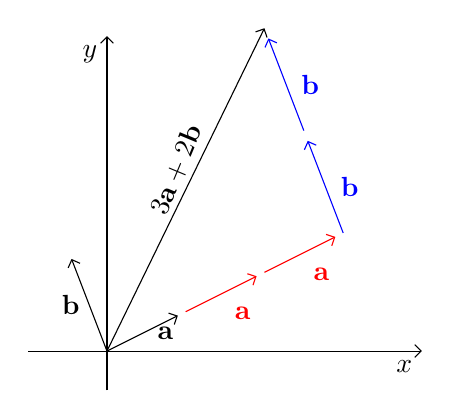
\begin{tikzpicture}[% styles used in image code
         > = Straight Barb, % defined in "arrows.meta
dot/.style = {circle, fill,
              minimum size=2mm, inner sep=0pt, outer sep=0pt,
              node contents={}},
box/.style = {draw, thin, minimum  width=2mm, minimum height=4mm,
              inner sep=0pt, outer sep=0pt,
              node contents={}, sloped},
my angle/.style args = {#1/#2}{draw,->,
                               angle radius=#1,
                               angle eccentricity=#2,
                               } % angle label position!
                        ]
	% coordinate axis
	\draw[->] (-1, 0) -- (4,0) node[below left] {$x$};
	\draw[->] ( 0,-0.5) -- (0,4) node[below left] {$y$};

	\coordinate (O) at (0,0);
	\coordinate (a) at (1,0.5);
	\coordinate (b) at (-0.5,1.3);
	
	\draw [->] (O) --($0.9*(a)$) node[pos=0.5,right=2pt] {$\mathbf{a}$};
	\draw [->,red] (a) --($1.9*(a)$) node[pos=0.5,below right=2pt] {$\mathbf{a}$};
	\draw [->,red] ($2*(a)$) --($2.9*(a)$) node[pos=0.5,below right=2pt] {$\mathbf{a}$};
	\draw [->] (O) --($0.9*(b)$) node[pos=0.5,left] {$\mathbf{b}$};
	\draw [->,blue] ($3*(a)$) --($3*(a) + 0.9*(b)$) node[pos=0.5,right=2pt] {$\mathbf{b}$};
	\draw [->,blue] ($3*(a) + (b)$) --($3*(a) + 1.9*(b)$) node[pos=0.5,right=2pt] {$\mathbf{b}$};
	\draw [->] (O) --($3*(a) + 2*(b)$) node[pos=0.7,above left, rotate=67.38] {$3\mathbf{a}+2\mathbf{b}$};
	%\draw [->] (a) --($(a)+1.3*(r)$) node[pos=0.9,above,rotate=26.5] {$\mathbf{a}}$};
\end{tikzpicture}
\end{figure}






\section{Vector subspaces and spans}

\definition{Vector subspace}{
Suppose that $V$ is a vector space and $W$ is a subset of $V$. We call $W$ a \textit{vector subspace} if it satisfies the vector space axioms for the same definition of vector addition and scalar multiplication defined for $V$.
}

\noindent In practice it can be tedious to show all 10 axioms hold for the subset. However, many of the properties are automatically inherited from the known vector space. For example any subset of vectors will obviously satisfy commutativity and associativity. In the end it suffices to prove just 3 properties for the candidate subspace.

\theorem{Demonstration of a vector subspace}{
Let $W$ be a subset of a vector space $V$. $W$ is a vector subspace if and only if
\begin{enumerate}
	\item $W$ is a non-empty set,
	\item $W$ is closed under vector addition: $\mathbf{u},\mathbf{v}\in W \, \implies \, \mathbf{u}+\mathbf{v}\in W$,
	\item $W$ is closed under scalar multiplication: $\mathbf{u}\in W \, \text{and} \, k\in\mathbb{R} \, \implies \, k\mathbf{u}\in W$.
\end{enumerate}
In fact, we can merge the two closure properties into one: closure under linear combinations
\begin{gather*}
\forall \mathbf{u},\mathbf{v}\in W \quad \text{and} \quad \forall \alpha, \beta\in\mathbb{R} \\
\alpha \mathbf{u} + \beta \mathbf{v} \in W.
\end{gather*}
}

\example{Vector subspace of triples satisfying an equation}{

\noindent Consider the equation $2x -y + z = 0$. We want to study the set of all triples, $(x,y,z)$, that satisfy the equation (we might call such a triple a ``solution'' to the equation). The set of these triples are a subset, call it $W$, of the Euclidean vector space $\mathbb{R}^3$. Let's show that $W$ is a vector subspace of $\mathbb{R}^3$. \\ 

\noindent Firstly, the vector $(0,0,0)\in W$ because its components satisfy the equation: $2(0)-(0)+(0)$ indeed equals zero. Hence $W$ has at least one vector, that is, it is a non-empty set (it's also easy to see that, for example, $(1,1,-1)$ or $(1,2,0)$ are also members of $W$). Let $\mathbf{u}=(u_x, u_y, u_z)$ and $\mathbf{v}=(v_x, v_y, v_z)$ be two arbitrary triples in $W$. That means their components satisfy the equation, i.e. $2u_x -u_y + u_z = 0$ and $2v_x -v_y + v_z = 0$. For any real $\alpha$ and $\beta$ we therefore have
\begin{align*}
\alpha \mathbf{u} + \beta \mathbf{v} = (\alpha u_x + \beta v_x, \alpha u_y + \beta v_y, \alpha u_z + \beta v_z) = (w_x, w_y, w_z).
\end{align*}
We need to check whether the components of this resultant triple satisfies the defining equation of $W$.
\begin{align*}
2w_x -w_y + w_z &= 2(\alpha u_x + \beta v_x) - (\alpha u_y + \beta v_y) + \alpha u_z + \beta v_z \\
&= \alpha (\underbrace{2u_x -u_y + u_z}_{=0}) + \beta \underbrace{2v_x -v_y + v_z}_{=0}.
\end{align*}
Since the triple $\alpha \mathbf{u} + \beta \mathbf{v}$ has components satisfying the equation, we conclude that $\alpha \mathbf{u} + \beta \mathbf{v} \in W$. So $W$ is a non-empty subset of a vector space and $W$ is closed under linear combinations. Thus $W$ is a vector subspace.
}


\example{Vector subspace of functions satisfying a equation}{

\noindent Let $W$ be the set of solutions of the following differential equation
\begin{align*}
\frac{d^2 y}{dx^2} + 3 \frac{dy}{dx} - 2y = 0.
\end{align*}
Is $W$ a vector subspace of the vector space of all real valued functions with real domain, $V$? \\

\noindent Consider the zero function $0(x) = 0$ for all $x\in\mathbb{R}$. This function's first and second derivatives combine to give
\begin{align*}
\frac{d^2}{dx^2}(0(x)) + 3 \frac{d}{dx}(0(x)) - 2(0(x)) = 0
\end{align*}
and so $0(x) \in W$, which is therefore a non-empty subset of $V$. If we have two functions, $y_1(x)$ and $y_2(x)$, in $V$ then they satisfy
\begin{align*}
\frac{d^2 y_1}{dx^2} + 3 \frac{dy_1}{dx} - 2y_1 = 0 \\
\frac{d^2 y_2}{dx^2} + 3 \frac{dy_2}{dx} - 2y_2 = 0.
\end{align*}
For any constants $\alpha$ and $\beta \in \mathbb{R}$ the linear combination of these solutions, $y=\alpha y_1+\beta y_2$, gives
\begin{align*}
\frac{d^2 y}{dx^2} + 3 \frac{dy}{dx} - 2y &= \frac{d^2}{dx^2}(\alpha y_1+\beta y_2) + 3 \frac{d}{dx}(\alpha y_1+\beta y_2) - 2(\alpha y_1+\beta y_2) \\
 &= \alpha\left(\frac{d^2 y_1}{dx^2} + 3 \frac{dy_1}{dx} - 2y_1\right) + \beta\left(\frac{d^2 y_2}{dx^2} + 3 \frac{dy_2}{dx} - 2y_2\right) \\
 &= 0
\end{align*}
and therefore $\alpha y_1+\beta y_2 \in W$. So we have shown that $W$ is a non-empty subset of $V$ which is closed under linear combinations. Hence $W$ is a vector subspace of $V$.
}

In the previous example we \textit{verified} that a space satisfied the vector space axioms. Now let's generate a vector space out of some given vectors. We can use the idea of linear combinations to generate a whole set of vectors.

\definition{Span}{
Let $\mathcal{B} = \{\mathbf{v}_1, \dots, \mathbf{v}_n\}$ be a set of vectors from a vector space $V$. The span of these vectors is the set of all linear combinations of those vectors:
\begin{align*}
\text{SPAN}(\mathcal{B})  = \text{SPAN} (\mathbf{v}_1, \dots, \mathbf{v}_n) = \left\{ \alpha_1 \mathbf{v}_1 + \cdots + \alpha_n \mathbf{v}_n \, | \, \alpha_1, \dots, \alpha_n \in \mathbb{R}^n \right\}.
\end{align*}
This set forms a vector subspace of $V$. It is obviously non-empty because it at least contains the vectors of $\mathcal{B}$. It is also automatically closed under vector addition and scalar multiplication because those are exactly the operations we used to create all the vectors in the span! Therefore $\text{SPAN}(\mathcal{B})$ is a vector subspace of $V$. \\

\noindent Note: we say that a set of vectors, $\mathcal{B}$, spans a vector space $U$ if $\text{SPAN}(\mathcal{B})=U$.
}




\example{Span of 1 vector}{
Suppose we have a vector space $V$. For any single arbitrary vector of $\mathcal{V}$ we can form the span subspace:
\begin{align*}
\textbf{v} \in V \quad\implies\quad \text{SPAN}(\textbf{v}) = \{k \textbf{v} \, | \, k\in\mathbb{R} \}
\end{align*}
If $V$ is $\mathbb{R}^2$, then this span is the line along the same direction of the arrow $\textbf{v}$:
\begin{figure}[H]
\centering
\begin{tikzpicture}[> = Triangle,scale=2]
	% coordinate axes
	\draw[->] (-1, 0) -- (3,0) node[right] {$x$};
	\draw[->] (0, -1) -- (0,2) node[left] {$y$};

	\coordinate (O) at (0,0); 
		
	% straight line y=x/2
	\draw[-,nicegreen,line width = 0.6mm] (-1,-0.5)--(3,1.5) node[left=10pt,darkgreen] {$\text{SPAN}(\textbf{v})$};
	
	% vectors u=(1,0.5) and v=(2,1)
	\draw[->,airforceblue,line width = 0.5mm] (O)--(1.2,0.6) node[below right,black] {$\textbf{v}=(x,y)$};
	%%%%%%%%%%%%%%%%%%%%%%%%%%%%%
\end{tikzpicture}
\end{figure}
\noindent If $V$ is, for example, the vector space of functions continuous on a given intervel, this span is a set of constant multiples of some function in $V$:
\begin{figure}[H]
\centering
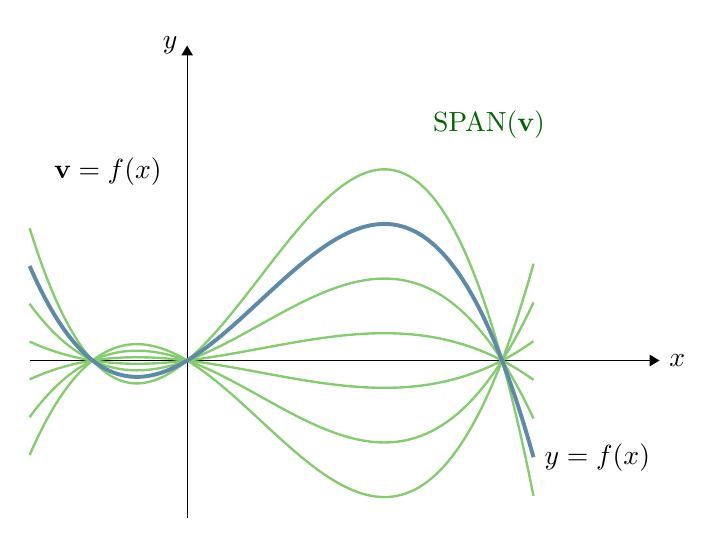
\begin{tikzpicture}[> = Triangle,scale=2]
	% coordinate axes
	\draw[->] (-1, 0) -- (3,0) node[right] {$x$};
	\draw[->] (0, -1) -- (0,2) node[left] {$y$};


	\coordinate (O) at (0,0); 
	\draw[smooth,variable=\x,samples=100,domain=-1:2.2,nicegreen,line width=0.3mm] plot({\x},{-0.7*(\x+0.6)*\x*(\x-2)});
	\draw[smooth,variable=\x,samples=100,domain=-1:2.2,nicegreen,line width=0.3mm] plot({\x},{-0.3*(\x+0.6)*\x*(\x-2)});
	\draw[smooth,variable=\x,samples=100,domain=-1:2.2,nicegreen,line width=0.3mm] plot({\x},{-0.1*(\x+0.6)*\x*(\x-2)});
	\draw[smooth,variable=\x,samples=100,domain=-1:2.2,nicegreen,line width=0.3mm] plot({\x},{+0.1*(\x+0.6)*\x*(\x-2)});
	\draw[smooth,variable=\x,samples=100,domain=-1:2.2,nicegreen,line width=0.3mm] plot({\x},{+0.3*(\x+0.6)*\x*(\x-2)});
	\draw[smooth,variable=\x,samples=100,domain=-1:2.2,nicegreen,line width=0.3mm] plot({\x},{+0.5*(\x+0.6)*\x*(\x-2)});
	\draw[smooth,variable=\x,samples=100,domain=-1:2.2,airforceblue,line width=0.5mm] plot({\x},{-0.5*(\x+0.6)*\x*(\x-2)}) node[right,black] {$y=f(x)$};
	
	\node[black,left] at (-0.1,1.2) {$\textbf{v}=f(x)$};
	\node[darkgreen,right] at (1.5,1.5) {$\text{SPAN}(\textbf{v})$};
	%%%%%%%%%%%%%%%%%%%%%%%%%%%%%
\end{tikzpicture}
\end{figure}
\noindent Of course these are not all of the functions in the span, as that would be a filled block of green. 
}

\noindent In 3d Euclidean space, the span of any two vectors pointing in different directions will form a plane. In the picture below we see some linear combinations of $\mathbf{a}$ and $\mathbf{b}$. Hopefully you can convince yourself that no such linear combination could leave the blue plane. We will prove this later.

\begin{figure}[H]
\centering
\tdplotsetmaincoords{105}{-30}
\begin{tikzpicture}[tdplot_main_coords,font=\sffamily]
  \tdplotsetrotatedcoords{00}{30}{0}
  \begin{scope}[tdplot_rotated_coords]
  \begin{scope}[canvas is xy plane at z=0]
    \fill[blue,fill opacity=0.1] (-3.5,-5) rectangle (2,4); 
    \path (-150:2) coordinate (H) (-1.5,0) coordinate(X);
   
    \coordinate (O) at (0,0);
    \coordinate (a) at (-1,1.8);
    \coordinate (b) at (-2,-1);
    \draw [->,red] (O) --($(a)$) node[pos=0.6,below=1pt] {$\mathbf{a}$};
    \draw [->,red] (O) --($(b)$) node[pos=0.6,right=1pt] {$\mathbf{b}$};
    
    \draw [->] (O) --($(a)+(b)$) node[pos=1,above=1pt] {$\mathbf{a}+\mathbf{b}$};
    \draw [->,blue] ($(a)+0.05*(b)$) --($(a)+0.9*(b)$) node[pos=0.5,left=1pt] {$\mathbf{b}$};
    
    \draw [->] (O) --($(b)-2*(a)$) node[pos=1,right=1pt] {$\mathbf{b}-2\mathbf{a}$};
    \draw [->,blue] ($(a)-0.1*1.2*(b)$) --($(a)-0.9*1.2*(b)$) node[pos=0.8,left=1pt] {$-1.2\mathbf{b}$};
    
    \draw [->] (O) --($(a)-1.2*(b)$) node[pos=1,right=1pt] {$\mathbf{a}-1.2\mathbf{b}$};
    \draw [->,blue] ($(b)-0.1*2*(a)$) --($(b)-0.9*2*(a)$) node[pos=0.7,above=1pt] {$-2\mathbf{a}$};
    
   
   \pgflowlevelsynccm
  \end{scope} 
 \end{scope}
 \pgfmathsetmacro{\Radius}{1.5}
 
 
 \draw[-stealth] (O)-- (2.5*\Radius,0,0) node[pos=1.15] {$y$};
 \draw[-stealth] (O) -- (0,3.5*\Radius,0) node[pos=1.15] {$x$};
 \draw[-stealth] (O) -- (0,0,2.5*\Radius) node[pos=1.05] {$z$};
\end{tikzpicture}\caption*{Some selected linear combinations, the black arrows, of $\mathbf{a}$ and $\mathbf{b}$.}
\end{figure}



\example{Checking whether a vector belongs to a span}{

\noindent Let $\mathbf{u}=(1,1,2)$ and $\mathbf{v}=(0,3,1)$ be two Euclidean vectors. Let $\text{SPAN}(\mathbf{u},\mathbf{v})=V$. Does the vector $\mathbf{w}=(1,-5,0)$ belong to $V$? \\

\noindent We need to check whether $\mathbf{w}$ really is a linear combination of $\mathbf{u}$ and $\mathbf{v}$ or not. If it is, then we can write:
\begin{align*}
\mathbf{w} = \alpha \mathbf{u} + \beta \mathbf{v}
\end{align*}
for some $\alpha$ and $\beta$ that we can find or else we will find a contradiction. We have assumed
\begin{align*}
(1,-5,0) &= \alpha(1,1,2) + \beta (0,3,1) \\
&= (\alpha,\alpha + 3\beta,2\alpha+\beta)
\end{align*}
giving the 3 equations
\begin{align*}
\alpha=1, \quad \alpha + 3\beta=-5, \quad 2\alpha+\beta = 0
\end{align*}
Putting the value of $\alpha$ into either the second or third gives the same result: $\beta = -2$. Importantly $(\alpha,\beta)=(1,-2)$ does not contradict the second equation. Hence $\mathbf{w}$ is a linear combination of $\mathbf{u}$ and $\mathbf{v}$
\begin{align*}
\mathbf{w}=\mathbf{u}-2\mathbf{v}
\end{align*}
and therefore $\mathbf{w}\in V$. Note that if we had shown that $\alpha$ and $\beta$ were impossible to exist, then this would mean $\textbf{w} \notin V$.
}

\definition{Cartesian form of Euclidean vector subspaces}{
Euclidean vector sub spaces can always be written as a set with some defining equations, called the Cartesian form:
\begin{align*}
\left\{ (x_1,\dots,x_n) \in \mathbb{R}^n \, | \, \text{equations relating the } x_k \right\}.
\end{align*}
For example, the general form of planar vector subspaces of $\mathbb{R}^3$ is
\begin{align*}
V_P = \left\{ (x,y,z)\in \mathbb{R}^3 \, | \, ax + by + cz = 0\right\}
\end{align*}
where $a$, $b$ and $c$ are some given constants. This set is read aloud as ``all the triples $(x,y,z)$ such that $ax + by + cz = 0$''.
}


\example{Second method to check whether a vector belongs to a span}{

\noindent Let's take up the previous example and answer it with a second method. Let $\mathbf{u}=(1,1,2)$ and $\mathbf{v}=(0,3,1)$ be two Euclidean vectors. Let $\text{SPAN}(\mathbf{u},\mathbf{v})=V$. Does the vector $\mathbf{w}=(1,-5,0)$ belong to $V$? \\

\noindent First we'll find an equation that defines this span. By definition
\begin{align*}
V = \{\alpha \mathbf{u} + \beta \mathbf{v} \, | \, \alpha, \beta  \in \mathbb{R}\}.
\end{align*}
So a generic vector $(x,y,z)$ in $V$ must satisfy
\begin{align*}
(x,y,z) &= \alpha (1,1,2) + \beta (0,3,1).
\end{align*}
Let's look for a single equation relating the $x$, $y$ and $z$:
\begin{align*}
(x,y,z) =  (\alpha,\alpha + 3\beta,2\alpha + \beta) 
\implies
\begin{cases}
x=\alpha \\
y=\alpha + 3\beta \\
z=2\alpha + \beta
\end{cases}
\implies
\begin{cases}
x=\alpha \\
y=x + 3\beta \\
z=2x + \beta
\end{cases}
\implies
\begin{cases}
x=\alpha \\
y=x + 3\beta \\
y-3z=-5x
\end{cases}
\end{align*}
This last line gives us the equation that all vectors of $V$ must satisfy, and so we have its Cartesian form:
\begin{align*}
V = \{(x,y,z)\in\mathbb{R}^3 \, | \, 5x + y - 3z = 0 \}.
\end{align*}
With this equation we can easily check whether $\mathbf{w}=(1,-5,0)$ belongs to $V$ or not:
\begin{align*}
5w_x + w_y - 3w_z = 5(1)+(-5)-3(0) = 0.
\end{align*}
The equation is satisfied and so $\mathbf{w}\in V$.
}


\example{Span of two 3d vectors in Cartesian form}{

\noindent Given the vectors
\begin{align*}
\textbf{v}_1 = (3,-1,1) \quad\text{and}\quad \textbf{v}_2 = (1,2,0)
\end{align*}
what is the Cartesian form of the span of these vectors, SPAN($\textbf{v}_1,\textbf{v}_2$)? \\

\noindent Consider an arbitrary triple in this space: $(x,y,z) \in \text{SPAN}(\textbf{v}_1,\textbf{v}_2)$. To be in this span means to be a linear combination: 
\begin{align*}
(x,y,z) = \alpha\textbf{v}_1 + \beta\textbf{v}_2
\end{align*}
for constants $\alpha$, $\beta$. This can be expanded 
\begin{align*}
(x,y,z) = \alpha(3,-1,1) + \beta(1,2,0) = (3\alpha + \beta,-\alpha + 2\beta,\alpha)
\end{align*}
to give the system of equations
\begin{align*}
\begin{cases}
x = 3\alpha + \beta \\
y = -\alpha + 2\beta \\
z = \alpha 
\end{cases}
\quad\implies\quad
2x - y - 7z = 0
\end{align*}
Which finally means that we have the Cartesian form
\begin{align*}
\text{SPAN}(\,(3,-1,1),(1,2,0)\,) = \left\{(x,y,z)\in\mathbb{R}^3 \, | \, 2x - y - 7z = 0\right\}
\end{align*}
As $2x - y - 7z = 0$ is a plane equation, this span creates a planar vector space.
}

\theorem{Span of two 3d vectors gives a plane}{
For any two 3d Euclidean vectors, $\textbf{u},\textbf{v}\in \mathbb{R}^3$, if they do not point in the same direction ($\textbf{u}\neq k\textbf{v}$ for some constant $k$) then their span gives a planar vector subspace of $\mathbb{R}^3$.
}

\begin{proof}
Let $\mathbf{u}=(u_x,u_y,u_z)$, $\mathbf{v}=(v_x,v_y,v_z)$ and $(x,y,z)\in \text{SPAN}(\mathbf{u},\mathbf{v})$. Then we must have some constants $\alpha,\beta \in \mathbb{R}$ such that
\begin{align*}
(x,y,z) &= \alpha \mathbf{u} + \beta \mathbf{v} \\
&= (\alpha u_x + \beta v_x, \, \alpha u_y + \beta v_y, \, \alpha u_z + \beta v_z)
\end{align*}
So we have the system of equations
\begin{align*}
& \begin{cases}
x = \alpha u_x + \beta v_x \\
y = \alpha u_y + \beta v_y \\
z = \alpha u_z + \beta v_z
\end{cases}
\implies
\begin{cases}
u_y x = \alpha u_x u_y  + \beta v_x u_y  \\
u_x y = \alpha u_x u_y + \beta v_y u_x \\
u_x z = \alpha u_x u_z + \beta v_z u_x \\
u_z x = \alpha u_x u_z + \beta v_x u_z 
\end{cases}
\implies
\begin{cases}
u_y x - u_x y = \beta (v_x u_y - v_y u_x) \\
u_z x - u_x z = \beta (v_x u_z -  v_z u_x)
\end{cases} \\
& \implies
\begin{cases}
(u_y x - u_x y)(v_x u_z -  v_z u_x) = \beta (v_x u_y - v_y u_x)(v_x u_z -  v_z u_x) \\
(u_z x - u_x z)(v_x u_y - v_y u_x) = \beta (v_x u_z -  v_z u_x)(v_x u_y - v_y u_x)
\end{cases} \\
& \implies
(u_y x - u_x y)(v_x u_z -  v_z u_x) - (u_z x - u_x z)(v_x u_y - v_y u_x) = 0
\end{align*}
A final rearrangement gives us our plane equation
\begin{align*}
(v_y u_x u_z-  v_z u_x u_y)x + (v_z u_x^2 - v_x u_z u_x) y + (v_x u_y u_x - v_y u_x^2)z = 0
\end{align*}
\textit{Note}: if the two vectors pointed in the same direction, we could find a constant $k$ such that $\mathbf{v}=k\mathbf{u}$ which implies that $v_x=ku_x$, $v_y=ku_y$ and $v_z=ku_z$. Putting this into the plane equation gives
\begin{align*}
\underbrace{(ku_y u_x u_z-  ku_z u_x u_y)}_0x + \underbrace{(ku_z u_x^2 - ku_x u_z u_x)}_0 y + \underbrace{(ku_x u_y u_x - ku_y u_x^2)}_0z = 0
\end{align*}
Since the left side cancels to zero, we don't have a plane equation relating the $x$, $y$ and $z$ variables.
\end{proof}


\example{From Cartesian form to a span}{

\noindent Given the Cartesian form of a vector space
\begin{align*}
A = \left\{(x,y,z)\in\mathbb{R}^3 \, | \, x + 2y - 3z = 0\right\}
\end{align*}
write $A$ in the form of a span of vectors. \\

\noindent We can rearrange the equation to $x=3z-2y$. So, every vector in $A$ can be written
\begin{align*}
(x,y,z) &= (3z-2y, y, z) \\
&= (-2y, y, 0) + (3z, 0, z) \\
&= y(-2, 1, 0) + z(3, 0, 1)
\end{align*}
With no further equations relating $y$ and $z$ to each other, they are free variables. This means $y$ and $z$ can take on any value. This means every triple $(x,y,z)\in A$ can be written as some linear combination of the vectors $\textbf{v}=(-2,1,0)$ and $\textbf{u}=(3,0,1)$. That is
\begin{align*}
A = \text{SPAN}( \, (-2,1,0), \, (3,0,1) \, )
\end{align*}
}


\section{Intersection, union and sum of subspaces}
The span vector space let us generate vector spaces out of given vectors. Now we look at generating vector spaces out of other vector spaces. As vector spaces are sets, it's natural to first consider the normal ways of combining sets: the intersection and union.

\theorem{Intersection of vector subspaces is a vector subspace}{
Suppose $V$ is a vector space. If $U$ and $W$ are two vector subspaces of $V$, then their intersection $U \cap W$ is also a vector subspace of $V$.}

\begin{proof} Let's show the two sufficient properties:
\begin{enumerate}
\item Non-empty - $U$ and $W$ must both contain the zero vector of $V$. Hence their intersection also contains the zero vector, and is thus a non-empty subset of $V$.

\item Closure under linear combinations - Let $\textbf{a}, \textbf{b} \in U \cap W$ and $\alpha, \beta \in \mathbb{R}$. Then $\textbf{a}, \textbf{b} \in U$, which is closed under linear combinations by being a vector space, and so $\alpha\textbf{a}+\beta\textbf{b} \in U$. But $\textbf{a}, \textbf{b} \in W$ also, which is closed under linear combinations, and so $\alpha\textbf{a}+\beta\textbf{b} \in W$. Hence
\begin{align*}
\alpha\textbf{a}+\beta\textbf{b} \in U\cap W
\end{align*}
and we have that the intersection is a vector subspace.
\end{enumerate}
\end{proof} 



For a visual example, consider the intersection of two planes in $\mathbb{R}^3$, $U$ and $V$, as pictured below.

\begin{figure}[H]
\begin{center}
    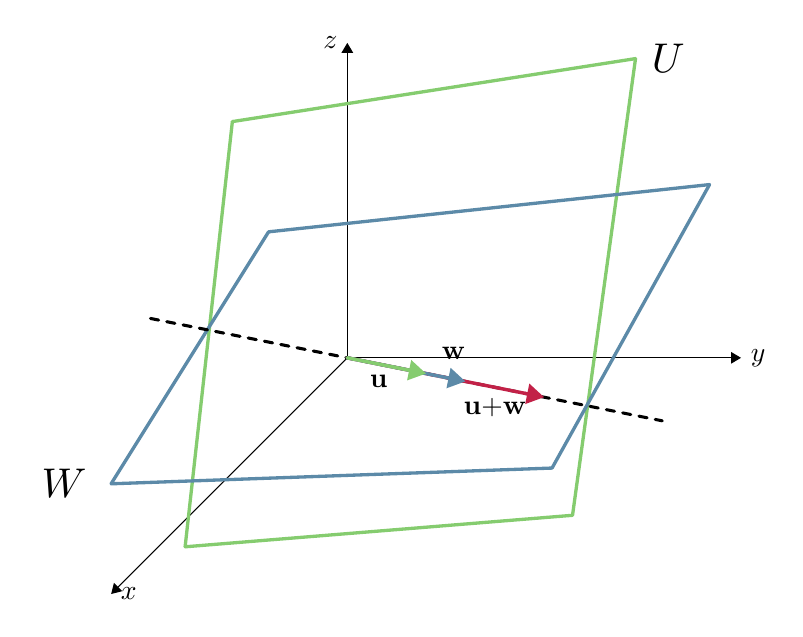
\begin{tikzpicture}[line cap=round, line join=round, >=Triangle,scale=2]

		% coordinate system
		\coordinate (O) at (0,0);
		\draw [->,black] (O)--(-1.5,-1.5) node[right] {$x$}; % x-axis
		\draw [->,black] (O)--(+2.5,+0.0) node[right] {$y$}; % y-axis
		\draw [->,black] (O)--(+0.0,+2.0) node[left] {$z$}; % z-axis
    
	    % plane 1 vertices positions
    	\coordinate (A1) at (-1.03,-1.2);
    	\coordinate (B1) at (-0.73,+1.5);
    	\coordinate (C1) at (+1.83,+1.9);
    	\coordinate (D1) at (+1.43,-1.0);
    	
	    % plane 2 vertices positions
    	\coordinate (A2) at (-1.5,-0.8);
    	\coordinate (B2) at (-0.5,+0.8);
    	\coordinate (C2) at (+2.3,+1.1);
    	\coordinate (D2) at (+1.3,-0.7);
    	
		\draw [-,nicegreen,line width=1.2pt] (A1)--(B1);
		\draw [-,nicegreen,line width=1.2pt] (B1)--(C1) node[right,black,pos=1,scale=1.5] {$U$};
		\draw [-,nicegreen,line width=1.2pt] (C1)--(D1);
		\draw [-,nicegreen,line width=1.2pt] (D1)--(A1);
    	
		\draw [-,airforceblue,line width=1.2pt] (A2)--(B2)node[left=3pt,black,pos=0,scale=1.5] {$W$};
		\draw [-,airforceblue,line width=1.2pt] (B2)--(C2);
		\draw [-,airforceblue,line width=1.2pt] (C2)--(D2);
		\draw [-,airforceblue,line width=1.2pt] (D2)--(A2);

		% vectors
		\coordinate (u) at (0.5,-0.1);
		\coordinate (w) at ($1.5*(u)$);
		\draw [dashed,black,line width=1.1pt] ($-2.5*(u)$)--($4*(u)$);
		\draw [->,brightmaroon,line width=1.25pt] (O)--($(u)+(w)$) node[below,black,pos=0.75] {\textbf{u}+\textbf{w}};
		\draw [->,airforceblue,line width=1.25pt] (O)--(w) node[above=3pt,black,pos=0.9] {\textbf{w}};
		\draw [->,nicegreen,line width=1.25pt] (O)--(u) node[below,black,pos=0.4] {\textbf{u}};
    \end{tikzpicture}
\end{center}
\end{figure}
The two planes must cross through $(0,0,0)$ to be subspaces (why?). The line of intersection will be a new subspace of $\mathbb{R}^3$. Of course any two vectors on this line will add up to a new vector still on the line.


\theorem{Union of vector subspaces}{
Suppose $V$ is a vector space. If we have 2 subspaces $U$ and $W$, then either
\begin{enumerate}
\item $U$ is a subspace of $W$
\item $W$ is a subspace of $U$
\item The union of $U$ and $W$ is NOT a subspace of $V$.
\end{enumerate}
}


\noindent To illustrate the third point, consider two straight lines in $\mathbb{R}^2$, $U$ and $V$.

\begin{figure}[H]
\begin{center}
    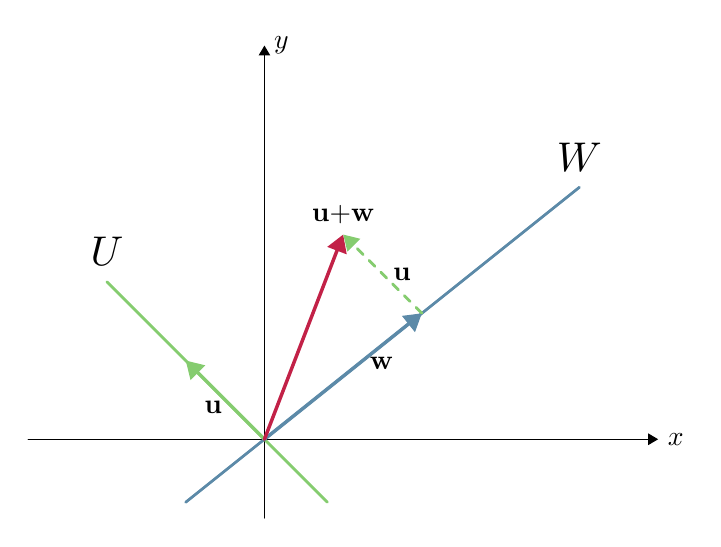
\begin{tikzpicture}[line cap=round, line join=round, >=Triangle,scale=2]
		% coordinate system
		\coordinate (O) at (0,0);
		\draw [->,black] (-1.5,0)--(+2.5,0) node[right] {$x$}; % x-axis
		\draw [->,black] (0,-0.5)--(0,+2.5) node[right] {$y$}; % y-axis
		
    	\coordinate (u) at (-0.5,+0.5);
    	\coordinate (w) at (1,0.8);
    	
		\draw [-,nicegreen,line width=1pt] ($-0.8*(u)$)--($2*(u)$) node[above,black,pos=1,scale=1.5] {$U$};
    	\draw [-,airforceblue,line width=1pt] ($-0.5*(w)$)--($2*(w)$) node[above,black,pos=1,scale=1.5] {$W$};
		
		\draw [->,nicegreen,line width=1.25pt] (O)--(u) node[left,black,pos=0.4] {\textbf{u}};
		\draw [->,airforceblue,line width=1.25pt] (O)--(w) node[right,black,pos=0.6] {\textbf{w}};
    	\draw [->,brightmaroon,line width=1.25pt] (O)--($(u)+(w)$) node[above,black] {\textbf{u}+\textbf{w}};
    	\draw [->,dashed,nicegreen,line width=1.0pt] (w)--($(u)+(w)$) node[right,black,pos=0.5] {$\textbf{u}$};

    \end{tikzpicture}
\end{center}
\end{figure}

\noindent The two lines must cross through $(0,0)$ to be subspaces. Remember that the union of two sets are all the members of both sets. For these two lines, the union will not be a new subspace of $\mathbb{R}^2$ because it is clearly not closed under vector addition. A simple example of this lack of closure is shown: any $\textbf{u}+\textbf{v}$ for $\textbf{u}\in U$ and $\textbf{v}\in V$ (and not the zero vectors) is clearly not going to remain in either $U$ or $V$.



\definition{Sum of subspaces (sum space)}{

Suppose we have a vector space $V$ with vector subspaces $F$ and $G$. We define the \textbf{sum of subspaces} (or sum space) as a new set denoted
\begin{align*}
F + G = \left\{ \textbf{f} + \textbf{g} \, | \, \textbf{f}\in F, \, \textbf{g}\in G\right\}
\end{align*}

\textit{Note}: The sum space is a \textit{subset} of the parent vector space: $F+G \subset V$.
}


\theorem{Sum space is a vector subspace}{
Let $F$ and $G$ be vector subspaces of $V$. The sum space $F+G$ is also a vector subspace of $V$.
}

\begin{proof} Let's show the two sufficient properties:
\begin{enumerate}
\item Non-empty. As $F$ is a vector space it must have at least the zero vector $\textbf{0}_V$. As $G$ is a vector space it cannot be empty, so it has at least some vector $\textbf{g}\in G$ (this could possibly be only the zero vector). The addition of these two vectors must be in the sum space: $\textbf{0}_V+\textbf{g}=\textbf{g}\in F+G$. So $F+G$ is not empty.

\item Closure. Let $\textbf{v}$ and $\textbf{w} \in F+G$ and $\alpha,\beta \in \mathbb{R}$. By definition the vectors can be written as the sum of vectors in $F$ and $G$: $\textbf{v}=\textbf{f}_1+\textbf{g}_1$ and $\textbf{w}=\textbf{f}_2+\textbf{g}_2$. The linear combination is thus
\begin{align*}
\alpha \textbf{v} + \beta \textbf{w} = \alpha\textbf{f}_1+\beta\textbf{f}_2+\alpha\textbf{g}_1+\beta\textbf{g}_2
\end{align*}
As $F$ and $G$ are vector spaces, they are closed under linear combinations. So $\alpha\textbf{f}_1+\beta\textbf{f}_2\in F$ and $\alpha\textbf{g}_1+\beta\textbf{g}_2 \in G$. Hence $\alpha \textbf{v} + \beta \textbf{w} = \textbf{f} + \textbf{g}$ for some $\textbf{f}\in F$ and $\textbf{g}\in G$, and thus $\alpha \textbf{v} + \beta \textbf{w} \in F+G$.
\end{enumerate}
\end{proof}


\noindent For a visual example of the sum of two subspaces. Consider two lines in $\mathbb{R}^2$ that pass through the origin. As we saw earlier that their union is not a vector subspace. But the sum of the two subspaces ($U$ and $W$ in the picture) includes all the possible vectors that can be reached by a sum of a vector belonging to each line:

\begin{figure}[H]
\begin{center}
    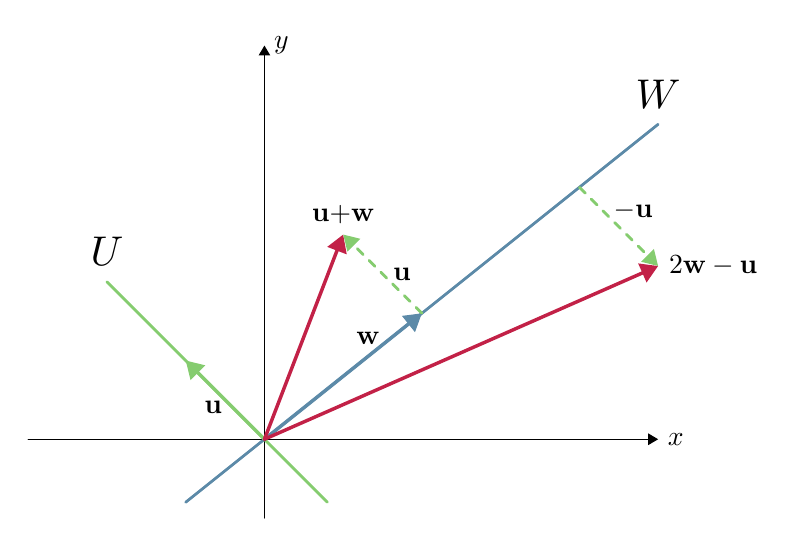
\begin{tikzpicture}[line cap=round, line join=round, >=Triangle,scale=2]
		% coordinate system
		\coordinate (O) at (0,0);
		\draw [->,black] (-1.5,0)--(+2.5,0) node[right] {$x$}; % x-axis
		\draw [->,black] (0,-0.5)--(0,+2.5) node[right] {$y$}; % y-axis
		
    	\coordinate (u) at (-0.5,+0.5);
    	\coordinate (w) at (1,0.8);
    	
		\draw [-,nicegreen,line width=1pt] ($-0.8*(u)$)--($2*(u)$) node[above,black,pos=1,scale=1.5] {$U$};
    	\draw [-,airforceblue,line width=1pt] ($-0.5*(w)$)--($2.5*(w)$) node[above,black,pos=1,scale=1.5] {$W$};
		
		\draw [->,nicegreen,line width=1.25pt] (O)--(u) node[left,black,pos=0.4] {$\textbf{u}$};
		\draw [->,airforceblue,line width=1.25pt] (O)--(w) node[left,black,pos=0.8] {$\textbf{w}$};
    	\draw [->,brightmaroon,line width=1.25pt] (O)--($(u)+(w)$) node[above,black] {\textbf{u}+\textbf{w}};
    	\draw [->,dashed,nicegreen,line width=1.0pt] (w)--($(u)+(w)$) node[right,black,pos=0.5] {$\textbf{u}$};
    	\draw [->,dashed,nicegreen,line width=1.0pt] ($2*(w)$)--($-1*(u)+2*(w)$) node[right,black,pos=0.3] {$-\textbf{u}$};
    	\draw [->,brightmaroon,line width=1.25pt] (O)--($-1*(u)+2*(w)$) node[right,black] {$2\textbf{w}-\textbf{u}$};

    \end{tikzpicture}
\end{center}
\end{figure}
\noindent Incidentally, in this example, the vector space $U + W$ is equal to all $\mathbb{R}^2$.

You should ask yourself ``how is the sum space different to the span''? The concept of sum space will later let us understand how to decompose vector spaces into constituent \textit{vector spaces}, whereas the span let's us consider the \textit{vectors} themselves as the generating objects.

\theorem{Smallest vector space containing a union of vector spaces}{
Let $F$ and $G$ be vector subspaces of a vector space $V$. Then $F+G$ is the smallest vector subspace of $V$ that contains the union $F \cup G$.
}

\definition{Direct sum}{
Let $F$ and $G$ be two vector subspaces of a vector space $V$ and let $E=F+G$ be the sum space. We say $E$ is a \textbf{direct sum} of $F$ and $G$ if each element of $E$ has a \textbf{unique} decomposition as a sum of vectors in $F$ and vectors in $G$. That is, for every $\textbf{v}\in E$, there exists unique vectors $\textbf{f}\in F$ and $\textbf{g}\in G$ such that $\textbf{v} = \textbf{f} + \textbf{g}$. We denote this direct sum with a new symbol
\begin{align*}
E = F \oplus G
\end{align*}
}

\noindent Lets build intuition by starting with an example of a sum space that is not a direct sum. 

\example{Sum of two planar vector spaces}{
Consider the following two vector subspaces of $\mathbb{R}^3$
\begin{align*}
A = \left\{ (x,y,z) \in\mathbb{R}^3 \, | \, x+y+z=0  \right\} \quad\text{and}\quad
B = \left\{ (x,y,z) \in\mathbb{R}^3 \, | \, x-y+z=0  \right\}.
\end{align*}
Is $A+B$ a direct sum of $A$ and $B$? \\

\noindent Let $\textbf{v}$ be an arbitrary vector in the sum space $A+B$. Then we have
\begin{align*}
\textbf{v}= (x,y,z) = \textbf{a} + \textbf{b}
\end{align*}
for some $\textbf{a}=(a_x,a_y,a_z)\in A$ and $\textbf{b}=(b_x,b_y,b_z)\in B$. So we can write the system of 5 equations with 6 unknowns 
\begin{align*}
x &= a_x + b_x &\quad a_x + a_y + a_z = 0\\
y &= a_y + b_y &\quad b_x - b_y + b_z = 0 \\
z &= a_z + b_z
\end{align*}
Now the goal is to invert these equations to find $a_x$, $a_y$, $a_z$, $b_x$, $b_y$ and $b_z$ as functions of $x$, $y$ and $z$. We don't have enough equations to do this uniquely, so we end up with a free variable. There are infinite ways to write this, but lets look at the solution if we let $b_z=t$ for any $t\in \mathbb{R}$:
\begin{align*}
a_x &= \dfrac{x-y-z+2t}{2}, &\quad a_y &= \dfrac{-x+y-z}{2}, &\quad a_z &= z-t  \\
b_x &= \dfrac{x+y+z-2t}{2}, &\quad b_y &= \dfrac{x+y+z}{2},  &\quad b_z &= t
\end{align*}
Let's consider the triple $(1,1,1)$. We have
\begin{align*}
(1,1,1) &= \overbrace{\left(-\dfrac{1}{2},\, -\dfrac{1}{2}, \, 1\right)}^{\in A} + \overbrace{\left( \dfrac{3}{2}, \, \dfrac{3}{2}, \,0 \right)}^{\in B}, \quad \text{for t=0} \\
(1,1,1) &= \underbrace{\left( \dfrac{1}{2},\, -\dfrac{1}{2},\, 0\right)}_{\in A} + \underbrace{\left (\dfrac{1}{2}, \, \dfrac{3}{2}, \, 1 \right)}_{\in A}, \quad  \text{for t=1}.
\end{align*}
This shows we have 2 different sum decompositions of $(1,1,1)$. So $A+B$ cannot be a direct sum of $A$ and $B$ as we don't have \textit{unique} decompositions for all its vectors.
}

\noindent Now showing that a particular sum of subspaces gives rise to \textit{unique} sum decompositions is not necessarily straight forward. The next theorem gives us an easy method.

\theorem{Direct sum demonstration}{
Let $F$ and $G$ be two vector subspaces of $V$. Then $E=F+G$ is a direct sum of $F$ and $G$ if and only if the intersection of $F$ and $G$ contains only the zero vector:
\begin{align*}
F \cap G = \{\textbf{0}_V \}.
\end{align*}
}

\example{Intersection of two planes}{
Consider again the previous two vector subspaces of $\mathbb{R}^3$
\begin{align*}
A = \left\{ (x,y,z) \in\mathbb{R}^3 \, | \, x+y+z=0  \right\} \quad\text{and}\quad
B = \left\{ (x,y,z) \in\mathbb{R}^3 \, | \, x-y+z=0  \right\}.
\end{align*}
The defining equations of these sets are both planar equations. Thinking geometrically, the intersection of two planes is a line. So it's trivial to know $A \cap B \neq \{ (0,0,0)\}$. Let's show in detail exactly what this intersection set is.
\begin{align*}
A \cap B = \left\{ (x,y,z) \in\mathbb{R}^3 \, | \, x+y+z=0, \, x-y+z=0 \right\}
\end{align*}
These two equations as a system will have to be reduced. Adding them gives $x+z=0 \implies z = -x$. Subtracting them gives $y=0$. So every triple can be written $(x,y,z)=(x,0,-x)=(1,0,-1)x$ for arbitrary $x$. Thus the intersection is
\begin{align*}
A \cap B = \left\{ (1,0,-1)t \in\mathbb{R}^3 \, , \, \forall t\in \mathbb{R} \right\}= \text{SPAN}( \, (1,0,-1) \, )
\end{align*}
This set represents a straight line in the direction of $(1,0,-1)$. We expected a straight line when we take the intersection of two planes. Since the intersection contains more than just the zero vector, this shows that $A+B$ is not a direct sum of $A$ and $B$.
}



\example{Direct sum of a planar and a linear vector space}{

\noindent Consider the following two vector subspaces of $\mathbb{R}^3$
\begin{align*}
F = \left\{ (x,y,z) \in\mathbb{R}^3 \, | \, x+2y-z=0  \right\} \quad\text{and}\quad
G = \text{SPAN}( \, (2,0,1) \, ).
\end{align*}
Show that $\mathbb{R}^3$ is a direct sum of $F$ and $G$. \\

\noindent First we have to convert $G$ from vector form into Cartesian form (left as an exercise): 
\begin{align*}
G = \left\{ (x,y,z) \in\mathbb{R}^3 \, | \, y=0, \, x=2z \right\}
\end{align*}
Which gives the first representation of the intersection set 
\begin{align*}
F \cap G = \left\{ (x,y,z) \in\mathbb{R}^3 \, | \, x+2y-z=0, \, y=0, \, x=2z \right\}
\end{align*} 
Now we reduce the system of equations
\begin{align*}
\begin{cases}
x+2y-z=0 \\ y=0 \\ x=2z 
\end{cases}
\implies
\begin{cases}
x-z=0  \\ y=0 \\ x=2z 
\end{cases}
\implies
\begin{cases}
x=z \\ y=0  \\ x=2z 
\end{cases}
\end{align*}
The two equations $x=z$ and $x=2z$ imply $x=0$ and $z=0$. So we have shown that all 3 variables are necessarily zero. Hence
\begin{align*}
F \cap G = \left\{ (0,0,0)  \right\} = \left\{ \textbf{0}_{\mathbb{R}^3} \right\}
\end{align*} 
Let's now show that $F+G=\mathbb{R}^3$. Let $(x,y,z)\in \mathbb{R}^3$. We have to show that it is possible to write
\begin{align*}
(x,y,z) = (\alpha,\beta,\gamma) + (a,b,c)
\end{align*}
where $(\alpha,\beta,\gamma)\in F$ and $(a,b,c)\in G$. Expanding we get the equations
\begin{align*}
x = \alpha + a, \quad y = \beta + b, \quad z = \gamma + c \\
\alpha+2\beta-\gamma=0, \quad  b=0, \quad a=2c
\end{align*}
We want to rearrange these equations to know what $\alpha$, $\beta$, $\gamma$, $a$, $b$ and $c$ must be for a given triple $x$, $y$ and $z$.
\begin{align*}
\begin{cases}
x = \alpha + 2c \\
y = \beta \\
z = \gamma + c
\end{cases}
\implies
\begin{cases}
x + 2y - z =  \alpha + 2c + 2\beta - \gamma - c = c\\
x - 2z = \alpha - 2\gamma = \alpha - 2(\alpha+2\beta) = -\alpha-4y
\end{cases}
\end{align*}
So we have
\begin{align*}
\alpha = -x-4y + 2z, \quad \beta=y, \quad \gamma=-x-2y + 2z \\
a = 2x+4y-2z, \quad b=0, \quad c=x+2y-z
\end{align*}
and hence we can write any triple as the addition of vectors from $F$ and $G$
\begin{align*}
(x,y,z) = \underbrace{(-x-4y + 2z, \, y, \, -x-2y + 2z )}_{\in F} + \underbrace{(2x+4y-2z, \, 0, \, x+2y-z)}_{\in G}
\end{align*}
This shows $\mathbb{R}^3 \subset F + G$. Since it is trivial that $F+G \subset \mathbb{R}^3$, we have shown that $F+G=\mathbb{R}^3$. Adding that with $F \cap G  = \left\{ \textbf{0}_{\mathbb{R}^3} \right\}$, we have shown that $\mathbb{R}^3$ is a direct sum of $F$ and $G$: $\mathbb{R}^3=F \oplus G$.

\textit{Note}: the definition of the direct sum was about the sum space having \textit{unique} representations of the parent space. If you go through the proof closely, you can understand that the expression we derived:
\begin{align*}
(x,y,z) = (-x-4y + 2z, \, y, \, -x-2y + 2z ) + (2x+4y-2z, \, 0, \, x+2y-z)
\end{align*}
is the only possibly expression for vectors in this sum space. So it means every triple has this \textit{unique} addition of a vector in $F$ with a vector in $G$. To show that we have a direct sum also included the proof of unique sum decompositions, so we wasted effort by looking at the intersection. In this sense, the investigation of the intersection of the member spaces of the sum is better suited for proving the negative proposition, that a particular sum is \textit{not} a direct sum.
}


\definition{Complementary vector subspaces}{
Let $F$ and $G$ be two vector subspaces of $V$. $F$ and $G$ are called \textbf{complementary} if $V$ is a direct sum of $F$ and $G$. That is, if and only if
\begin{itemize}
\item $V = F+G$, and
\item $F \cap G = \{\textbf{0}_V \}$
\end{itemize}

Two examples will reveal the subtlety of this definition:
\begin{itemize}
\item For $A=\{ (x,y,z)\in \mathbb{R}^3 \, | \, y=2x \}$ and $B=\{ (x,y,z)\in \mathbb{R}^3 \, | \, y=-x \}$ we do not have the direct sum $\mathbb{R}^3=A \oplus B$ despite the intersection being only the zero vector.

\item For $A=\{ (x,y)\in \mathbb{R}^2 \, | \, y=2x \}$ and $B=\{ (x,y)\in \mathbb{R}^2 \, | \, y=-x \}$ we do have the direct sum $\mathbb{R}^2=A \oplus B$.
\end{itemize}
}

\noindent Finally, we have now defined a new type of addition. Don't be fooled by the plus symbol, the sum space is a specific definition of addition of whole vector spaces. However, this operation has parallels to normal number addition. We list some of these properties below.

\properties{of vector space summation}{

\noindent Let $F$, $G$, and $H$ be vector subspaces of a vector space $V$. The sum space satisfies the following properties:
\begin{itemize}
\item Associativity: $F + (G + H) = (F + G) + H$
\item Commutativity: $F + G = G + F$
\item Null element: $F + \{\textbf{0}_V\} = F$
\end{itemize}
}

\noindent While these properties are familiar properties of addition, there are also differences. For example, for any vector subspace $F$, the sum space $F+F=F$ (can you prove this?). This means there is no normal sense of scalar multiplication of vector spaces.





%%%%%%%%%%%%%%%%%%%%%%%%%%%
%%%%%%%%%%%%%%%%%%%%%%%%%%%
%%%%%%%%%%%%%%%%%%%%%%%%%%%
\section{Linear independence, bases and coordinates}
%%%%%%%%%%%%%%%%%%%%%%%%%%%
%%%%%%%%%%%%%%%%%%%%%%%%%%%
%%%%%%%%%%%%%%%%%%%%%%%%%%%
\subsection*{Linear dependence and independence}

\noindent When we considered the span of two 3d vectors giving a plane I casually inserted an important qualification, that the two vectors \textit{are not in the same direction}. If we have two vectors $\mathbf{u}$ and $\mathbf{v}$ in the same direction then, for example, $\mathbf{v}=k\mathbf{u}$ for some real $k$. Then any linear combination of these two vectors gives a third vector
\begin{align*}
\mathbf{w} &= \alpha \mathbf{u} + \beta \mathbf{v} \\
&= \alpha \mathbf{u} + \beta k\mathbf{u} \\
&= \left(\alpha + \beta k\right) \mathbf{u}
\end{align*}
that is, $\mathbf{w}$ must also be in the same direction as $\mathbf{u}$. The span of these 2 vectors gives only vectors in this single direction. In this case we say that $\mathbf{u}$ and $\mathbf{v}$ are not independent vectors. One can be represented in terms of the other. Let's formalise this notion of vector dependence.

\definition{Linear dependence}{
A set of vectors $\{\mathbf{v}_1, \dots, \mathbf{v}_n\}$ from a vector space $V$ is said to be \textit{linearly dependent} if there exists a set of constants $\{ \alpha_1, \dots, \alpha_n \}$ \textit{not all zero} such that
\begin{align*}
\alpha_1 \mathbf{v}_1 + \cdots + \alpha_n \mathbf{v}_n = \mathbf{0}_V.
\end{align*}
\textit{Note}: the right hand side of the equation is the \textit{zero vector}, not the real number $0$.
}

\example{Linear dependence of two Euclidean vectors}{

\noindent Let $\mathbf{u}=(1,2)$ and $\mathbf{v}=(10.2,20.4)$. Show that $\mathbf{u}$ and $\mathbf{v}$ are linearly dependent. \\

\noindent To show this we must demonstrate that there are two constants, $a$ and $b$, such that $a\mathbf{u} + b\mathbf{v} = \mathbf{0}$. If this was true, we would have
\begin{align*}
& a(1,2) + b(10.2,20.4) = (0,0) \\
\implies & (a + 10.2b,2a + 20.4b) = (0,0)
\end{align*}
giving the system of equations
\begin{align*}
\begin{cases}
a + 10.2b = 0 \\
2a + 20.4b = 0
\end{cases}
\end{align*}
Both equations give the same relation between $a$ and $b$:
\begin{align*}
b = -\frac{a}{10.2}
\end{align*}
We are free to choose an $a$, for example if $a=10.2$ then $b=-1$ and we have
\begin{align*}
10.2 \mathbf{u} - 1 \mathbf{v} = \mathbf{0}
\end{align*}
showing that the two vectors are linearly dependent. This example show that the linear dependence of 2 vectors means that 1 vector is a scalar multiple of the other. In this example:
\begin{align*}
\mathbf{v} = 10.2 \mathbf{u}.
\end{align*}
}

\noindent How does this definition relate to what we understood earlier, that two vectors are dependent on each other if one can be expressed in terms of the other? Well, consider three vectors $\mathbf{u}$, $\mathbf{v}$ and $\mathbf{w}\in \mathbb{R}^3$. If there exists some constants $\alpha$, $\beta$ and $\gamma$, \textit{not all zero}, such that
\begin{align*}
\alpha \mathbf{u} + \beta \mathbf{v} + \gamma \mathbf{w} = \mathbf{0}_V
\end{align*}
then we can write the vector with the non-zero constant in terms of the other. For example suppose $\alpha \neq 0$, then
\begin{align*}
\mathbf{u}  =-\frac{\beta}{\alpha} \mathbf{v} - \frac{\gamma}{\alpha} \mathbf{w}.
\end{align*}
In this way $\mathbf{u}$ depends on the other two, or we could say $\mathbf{u} \in \text{SPAN}(\mathbf{v},\mathbf{w})$. This also means that the span of the three vectors $\text{SPAN}(\mathbf{u},\mathbf{v},\mathbf{w})=\text{SPAN}(\mathbf{v},\mathbf{w})$. The vector $\mathbf{u}$ doesn't give anything new. 

For Euclidean vectors, when we have two vectors that are linearly dependent we say that they are \textit{colinear}, as pictured below.
\begin{figure}[H]
\begin{center}
    \begin{tikzpicture}[line cap=round, line join=round, >=Triangle,scale=2]
		% coordinate system
		\coordinate (O) at (0,0);
		\draw [->,black] (-1.5,0)--(+2.5,0) node[right] {$x$}; % x-axis
		\draw [->,black] (0,-0.5)--(0,+2.5) node[right] {$y$}; % y-axis
		
    	\coordinate (u) at (0.5,+0.4);
    	\coordinate (v) at (1.5,1.2);
    	
    	\draw [-,nicegreen,line width=1pt] ($-0.2*(v)$)--($2*(v)$)node[left=10pt,black,pos=0.8, scale=1.2] {$\text{SPAN}(\textbf{u},\textbf{v})$};
		
		\draw [->,brightmaroon,line width=1.25pt] (O)--(v) node[left,black,pos=0.8] {$\textbf{v}$};
		\draw [->,airforceblue,line width=1.25pt] (O)--(u) node[left=5pt,black,pos=0.8] {$\textbf{u}$};
    \end{tikzpicture}
\end{center}
\end{figure}

When we have three 3d Euclidean vectors that are linearly dependent we say that they are \textit{coplanar}. Any two of the vectors give a plane as their span and then adding the 3rd dependent vector gives linear combinations that remain in that plane, as pictured below.

\begin{figure}[H]
\begin{center}
    \begin{tikzpicture}[line cap=round, line join=round, >=Triangle,scale=2]

		% coordinate system
		\coordinate (O) at (0,0);
		\draw [->,black] (O)--(-1.5,-1.5) node[right] {$x$}; % x-axis
		\draw [->,black] (O)--(+2.5,+0.0) node[right] {$y$}; % y-axis
		\draw [->,black] (O)--(+0.0,+2.0) node[left] {$z$}; % z-axis
    
    	
	    % plane vertices positions
    	\coordinate (A) at (-1.5,-0.8);
    	\coordinate (B) at (-0.5,+0.8);
    	\coordinate (C) at (+2.3,+1.1);
    	\coordinate (D) at (+1.3,-0.7);
    	
    	
		\draw [-,airforceblue,line width=1.2pt] (A)--(B)node[left=3pt,black,pos=0,scale=1.2] {$\text{SPAN}(\textbf{u},\textbf{v},\textbf{w})$};
		\draw [-,airforceblue,line width=1.2pt] (B)--(C);
		\draw [-,airforceblue,line width=1.2pt] (C)--(D);
		\draw [-,airforceblue,line width=1.2pt] (D)--(A);

		% vectors
		\coordinate (u) at (0.5,-0.1);
		\coordinate (v) at (1,0.5);
		\coordinate (w) at (-0.5,0.2);
		\draw [->,nicegreen,line width=1.25pt] (O)--(u) node[below=3pt,black,pos=0.9] {$\textbf{u}$};
		\draw [->,airforceblue,line width=1.25pt] (O)--(v) node[above=3pt,black,pos=0.9] {$\textbf{v}$};
		\draw [->,brightmaroon,line width=1.25pt] (O)--(w) node[above=3pt,black,pos=0.9] {$\textbf{w}$};
    \end{tikzpicture}
\end{center}
\end{figure}

Now, what would it mean for a vector $\mathbf{u}$ to be independent of other vectors $\mathbf{v}$ and $\mathbf{w}$? The formal definition is simple:

\definition{Linear independence}{
A set of vectors $\{\mathbf{v}_1, \dots, \mathbf{v}_n\}$ from $V$ is said to be \textit{linearly independent} if they are not linearly dependent. That is, the equation
\begin{align*}
\alpha_1 \mathbf{v}_1 + \cdots + \alpha_n \mathbf{v}_n =  \mathbf{0}_V.
\end{align*}
implies that the constants $\alpha_1, \dots, \alpha_n$ \textit{are all zero}.
}

\noindent This definition is a little cheeky. Independent means not dependent. Let's understand it in the sense we were thinking earlier, where we think a vector $\mathbf{u}$ being independent of two other vectors $\mathbf{v}$ and $\mathbf{w}$ should mean that we cannot express $\mathbf{u}$ as a linear combination of $\mathbf{v}$ and $\mathbf{w}$. This follows from the definition. If we could write such a linear combination, then there are constants $\alpha$ and $\beta$ such that
\begin{align*}
\mathbf{u} &= \alpha \mathbf{u} + \beta \mathbf{v} \\
\implies & \mathbf{u}- \alpha \mathbf{u} - \beta \mathbf{v} = \mathbf{0}_V,
\end{align*}
but this equation is impossible as $\alpha_1 \mathbf{u} + \alpha_2 \mathbf{v} + \alpha_3 \mathbf{w} =  \mathbf{0}_V \implies \alpha_1=\alpha_2=\alpha_3=0$. \\


\example{Linear independence of three Euclidean vectors}{

\noindent Consider the following vectors in $\mathbb{R}^3$:
\begin{align*}
\mathbf{u} = (1,-1,1), \quad \mathbf{v} = (1,1,1), \quad \text{and} \quad \mathbf{w} = (2,2,4).
\end{align*}
Show that these three vectors are linearly independent. \\

\noindent We start with the equation
\begin{align*}
\alpha \mathbf{u} + \beta \mathbf{v} + \gamma \mathbf{w} = \mathbf{0}
\end{align*}
with the goal of finding possible solutions for $\alpha$, $\beta$ and $\gamma$. Writing the vector equation in full gives
\begin{align*}
& \alpha (1,-1,1) + \beta (1,1,1) + \gamma (2,2,4) = (0,0,0) \\
& (\alpha + \beta + 2\gamma, \, -\alpha + \beta + 2\gamma, \, \alpha + \beta + 4 \gamma) = (0,0,0)
\end{align*}
Component by component this vector equation is actually a system of equations
\begin{align*}
&\begin{cases}
\alpha + \beta + 2\gamma = 0 \\
-\alpha + \beta + 2\gamma = 0 \\
\alpha + \beta + 4\gamma = 0 
\end{cases}
\begin{matrix}
 \\
 L_2 \to L_2 + L_1 \\
 L_3 \to L_3 - L_1
\end{matrix}
\\
&\begin{cases}
\alpha + \beta + 2\gamma = 0 \implies \alpha = -\beta - 2\gamma \\
2\beta + 4\gamma = 0 \implies \beta = -2 \gamma \\
2\gamma = 0
\end{cases} 
\end{align*}
The last equation implies $\gamma=0$, which them implies $\beta=0$, which then implies $\alpha=0$. So the assumption that 
\begin{align*}
\alpha \mathbf{u} + \beta \mathbf{v} + \gamma \mathbf{w} = \mathbf{0}
\end{align*}
implies that $\alpha=\beta=\gamma=0$. That is exactly the definition of linear independence.
}


\example{Linear independence of three polynomial vectors}{

\noindent Consider the following vectors in the vector space of polynomials with degree up to two:
\begin{align*}
\mathbf{u} = 1 + x^2, \quad \mathbf{v} = x-2x^2, \quad \text{and} \quad \mathbf{w} = 3 - x.
\end{align*}
Show that these three vectors are linearly independent. \\

\noindent We start with the equation
\begin{align*}
\alpha \mathbf{u} + \beta \mathbf{v} + \gamma \mathbf{w} = \mathbf{0}
\end{align*}
with the goal of finding possible solutions for $\alpha$, $\beta$ and $\gamma$. Noting that the zero vector in the space of polynomials is the number 0, we write the vector equation in full
\begin{align*}
& \alpha ( 1 + x^2) + \beta (x-2x^2) + \gamma (3 - x) = 0 \\
& (\alpha + 3\gamma)1 + (\beta - \gamma)x + (\alpha - 2\beta)x^2 = (0)1 + (0)x + (0)x^2
\end{align*}
Equating the coefficients gives the system
\begin{align*}
\begin{cases}
\alpha + 3\gamma = 0 \implies \alpha = -\gamma/3 \\
\beta - \gamma = 0 \implies \beta = \gamma\\
\alpha - 2\beta = 0 \implies \alpha = 2\beta = 2\gamma
\end{cases}
\end{align*}
The only way that $\alpha = -\gamma/3$ and $\alpha = 2\gamma$ is for $\alpha=\gamma=0$. This then implies that $\beta=0$. We have therefore shown that
\begin{align*}
\alpha \mathbf{u} + \beta \mathbf{v} + \gamma \mathbf{w} = \mathbf{0}
\end{align*}
necessarily implies that $\alpha=\beta=\gamma=0$, and so these three vectors are linearly independent.
}

\noindent Take note of the simple logic or methodology of the previous three examples. We always start with the equation
\begin{align*}
\alpha_1 \mathbf{v}_1 + \alpha_2 \mathbf{v}_2 + \cdots + \alpha_n \mathbf{v}_n = \mathbf{0}_V
\end{align*}
and show either that by necessity all of the coefficients are zero (then the vectors are linearly independent), or that we can find at least one non-zero coefficients (then the vectors are linearly dependent). The exact method by which we determine these coefficients depends on which type of vectors we are considering.

\theorem{The span of a dependent set of vectors can be reduced}{
Let $\mathcal{B}=\{\mathbf{v}_1, \, \mathbf{v}_2, \, \dots, \mathbf{v}_n\}$ be a set of vectors of $V$. If $\mathcal{B}$ is a set of linearly dependent vectors, then we can always remove one of the vectors to form a new set, $\mathcal{B}'=\mathcal{B} \backslash \{\mathbf{v}_k\}$ for some $k$, without changing the span: $\text{SPAN}(\mathcal{B}')=\text{SPAN}(\mathcal{B})$.
}

\begin{proof}
Due to the linear dependence of the vectors of $\mathcal{B}$, there exists a set of constants $\alpha_1,\dots,\alpha_n \in \mathbb{R}$ not all zero such that
\begin{align*}
\alpha_1 \mathbf{v}_1 + \cdots + \alpha_n \mathbf{v}_n =  \mathbf{0}_V.
\end{align*}
Suppose $\alpha_k \neq 0$. Then we can write
\begin{align*}
\mathbf{v}_k = -\frac{\alpha_1}{\alpha_k} \mathbf{v}_1 - \cdots -\frac{\alpha_{k-1}}{\alpha_k} \mathbf{v}_{k-1} -\frac{\alpha_{k+1}}{\alpha_k}\mathbf{v}_{k+1} - \cdots -\frac{\alpha_n}{\alpha_k}  \mathbf{v}_n = -\sum_{i \neq k} \frac{\alpha_i}{\alpha_k} \mathbf{v}_i.
\end{align*}
which is to say $\mathbf{v}_k \in \text{SPAN}(\mathcal{B}')$ for $\mathcal{B}' = \left\{ \mathbf{v}_1, \, \cdots, \, \mathbf{v}_{k-1}, \,\mathbf{v}_{k+1}, \,  \mathbf{v}_n \right\}$. We want to prove that $\text{SPAN}(\mathcal{B}) = \text{SPAN}(\mathcal{B}')$. To show that two sets are equal we show that they are subsets of each other. That $ \text{SPAN}(\mathcal{B'}) \subset  \text{SPAN}(\mathcal{B})$ is trivial because $\mathcal{B}'$ is created out of $\mathcal{B}$ by only removing one vector. The other direction is more interesting. \\

\noindent Let $\mathbf{v} \in \text{SPAN}(\mathcal{B})$. Then we can find some set of constants $\beta_1$, \dots, $\beta_n$ not all zero such that
\begin{align*}
\mathbf{v} &= \beta_1 \mathbf{v}_1 + \cdots + \beta_k \mathbf{v}_k + \cdots + \beta_n \mathbf{v}_n \\
&= \beta_k \mathbf{v}_k + \sum_{i \neq k} \beta_i \mathbf{v}_i \\
&= \beta_k \left(-\sum_{i \neq k} \frac{\alpha_i}{\alpha_k} \mathbf{v}_i \right) + \sum_{i \neq k} \beta_i \mathbf{v}_i \\
&= \sum_{i \neq k} \left(\beta_i - \frac{\beta_k \alpha_i}{\alpha_k} \right)\mathbf{v}_i 
\end{align*}
This shows that $\mathbf{v}$ is a linear combination of vectors of $\mathcal{B}'$. So $\mathbf{v} \in \text{SPAN}(\mathcal{B}')$ and therefore $\text{SPAN}(\mathcal{B}) \subset  \text{SPAN}(\mathcal{B'})$.
\end{proof}


\noindent Now linear independence is a very important concept because it allows us to keep reducing the number of vectors in spans until we find a minimal set of vectors that are able to generate some vector space. Such a minimal set is called a basis, and is the focus of the next section.


\subsection*{Vector space basis}

\definition{Basis}{
A \textit{basis of a vector space} $V$ is a minimal set of vectors which spans the vector space. Formally, the set of vectors $\mathcal{B}=\{\mathbf{v}_1, \dots, \mathbf{v}_n\}$ in a vector space $V$ is a basis of $V$ if it is a set of linearly independent vectors and $\text{SPAN}(\mathbf{v}_1, \dots, \mathbf{v}_n) = V$. \textit{Note}: bases are not unique, but they always contain the same number of vectors.
}

\theorem{Bases of two dimensional Euclidean space}{
Any two linearly independent vectors in $\mathbb{R}^2$ forms a basis of $\mathbb{R}^2$.
}

\begin{proof}
Let $\mathbf{u}=(u_x,u_y)$ and $\mathbf{v}=(v_x,v_y)$ be two linearly independent vectors of $\mathbb{R}^2$. Since we've assumed the linear independence half of the definition of a basis, we only need to show that $\mathbb{R}^2 = \text{SPAN}(\mathbf{u},\mathbf{v})$. Let $(x,y)\in \mathbb{R}^2$. If $(x,y) \in \text{SPAN}(\mathbf{u},\mathbf{v})$ then we can find two constants $\alpha$ and $\beta \in \mathbb{R}$ such that
\begin{align*}
(x,y) &= \alpha \mathbf{u} + \beta \mathbf{v} \\
&= (\alpha u_x + \beta v_x, \,\alpha u_y + \beta v_y )
\end{align*}
which gives the system of equations
\begin{align*}
&
\begin{cases}
x = \alpha u_x + \beta v_x \\
y = \alpha u_y+ \beta v_y
\end{cases}
\\
\implies &
\begin{cases} 
u_y x - u_x y = (u_y  v_x  - u_x v_y) \beta \\
v_y x - v_x y = (v_y  u_x  - v_x u_y) \alpha
\end{cases}
\end{align*}
Now the linear independence of $\mathbf{u}$ and $\mathbf{v}$ means that the term in parentheses, $u_y  v_x  - u_x v_y$, is not zero. Why? Because if it was zero we would have
\begin{align*}
u_y  v_x = u_x v_y.
\end{align*}
We have some cases to consider here. If $v_y=0$, then either $u_y=0$ or $v_x=0$ (or both). 
\begin{itemize}
	\item If $v_x = 0$ then $\mathbf{v}=(0,0)=0\mathbf{u}$ and we have contradicted the assumption of linear independence. So we can't have $v_x = 0$.
	\item If $u_y=0$ then the two vectors become $\mathbf{u}=(u_x,0)$ and $\mathbf{v}=(v_x,0)$. Since $v_x$ cannot be zero we can write $\mathbf{u}=\dfrac{u_x}{v_x}\mathbf{v}$ and we have contradicted the assumption of linear independence. So we can't have $u_y=0$ . 
\end{itemize}
Since both outcomes are contradictions, we cannot have $v_y=0$. That is, we know $v_y\neq 0$. With that the equation $u_y  v_x = u_x v_y$ implies that neither $u_y$ nor $v_x$ can be zero and we can write
\begin{align*}
\frac{u_x}{u_y} = \frac{v_x}{v_y}.
\end{align*}
Then 
\begin{align*}
(u_x,u_y) &= u_y\left(\frac{u_x}{u_y},1\right) \\
          &= u_y\left(\frac{v_x}{v_y},1\right) \\
          &= \frac{u_y}{v_y}(v_x,v_y)
\end{align*}
and this contradicts the linear independence. So we simply can't have that $u_y  v_x  - u_x v_y=0$. All of that just so we can divide by this term, all the way back a long way to our system of equations to solve them for $\alpha$ and $\beta$:
\begin{align*}
 \alpha &= \frac{v_y x - v_x y}{v_y  u_x  - v_x u_y} \\
  \beta &= \frac{u_y x - u_x y}{u_y  v_x  - u_x v_y} 
\end{align*}
Now we can finally write any double in terms of $\mathbf{u}$ and $\mathbf{v}$:
\begin{align*}
(x,y) = \frac{v_y x - v_x y}{v_y  u_x  - v_x u_y}\mathbf{u} + \frac{u_y x - u_x y}{u_y  v_x  - u_x v_y} \mathbf{v}
\end{align*}
This shows that $\mathbb{R}^2 \subset \text{SPAN}(\mathbf{u},\mathbf{v})$. The other direction is automatic, and so we have proven that $\mathcal{B}=\{ \mathbf{u},\,\mathbf{v} \}$ is a basis of $\mathbb{R}^2$.
\end{proof}

\example{A basis of degree 1 polynomials}{

\noindent Consider a set of polynomial vectors $\mathcal{B}=\{ 1+x, \, 1-x \}$. Show that $\mathcal{B}$ is a basis of the vector space of polynomials with degree up to one, $\mathcal{P}_1$. \\

\noindent Let's start by showing the two vectors $\mathbf{b}_1 = 1+x$ and $\mathbf{b}_2=1-x$ are linearly independent. Assume
\begin{align*}
& \alpha \mathbf{b}_1 + \beta \mathbf{b}_2 = \mathbf{0} \\
\implies & \alpha (1+x) + \beta (1-x) = 0 \\
\implies & (\alpha + \beta)1 + (\alpha - \beta)x = (0)1 + (0)x
\end{align*}
which gives the system of equations
\begin{align*}
\begin{cases}
\alpha + \beta = 0 \\
\alpha - \beta = 0
\end{cases}
\end{align*}
Adding the equations gives $2\alpha = 0$ and subtracting gives $2\beta = 0$. So we have $\alpha=\beta=0$ and therefore $\mathbf{b}_1$ and $\mathbf{b}_2$ are linearly independent. Now let's prove that $\mathcal{P}_1 = \text{SPAN}(\mathbf{b}_1,\mathbf{b}_2)$. $\text{SPAN}(\mathbf{b}_1,\mathbf{b}_2) \subset \mathcal{P}_1$ is automatic. For the other direction, let $\mathbf{p}=(a)1+(b)x \in \mathcal{P}_1$ for some $a$, $b \in \mathbb{R}$. Then we want to find some $\alpha$, $\beta \in \mathbb{R}$ such that
\begin{align*}
\mathbf{p} &= \alpha\mathbf{b}_1+\beta\mathbf{b}_2 \\
\implies (a)1+(b)x &= \alpha (1+x) + \beta (1-x) \\
&= (\alpha + \beta)1 + (\alpha - \beta)x
\end{align*} 
and so
\begin{align*}
& \begin{cases}
a = \alpha + \beta \\
b = \alpha - \beta
\end{cases}
\\
\implies &
\begin{cases}
a+b = 2\alpha\\
a-b = 2\beta
\end{cases}
\\
\implies &
\begin{cases}
\alpha = \dfrac{a+b}{2} \\
\beta = \dfrac{a-b}{2} 
\end{cases}
\end{align*}
So we can write any polynomial of degree up to 1 in terms of the vectors in $\mathcal{B}$:
\begin{align*}
(a)1+(b)x = \frac{a+b}{2}\mathbf{b}_1 + \frac{a-b}{2}\mathbf{b}_2
\end{align*}
Therefore $ \mathcal{P}_1 \subset \text{SPAN}(\mathbf{b}_1,\mathbf{b}_2)$. We have therefore shown the two results
\begin{itemize}
\item $\mathcal{B}$ is a set of linearly independent vectors.
\item $\mathcal{B}$ spans $\mathcal{P}_1$.
\end{itemize}
which proves that $\mathcal{B}$ is a basis of $\mathcal{P}_1$.
}


\example{Basis of $\mathbb{R}^3$}{

\noindent Consider the set of 3 vectors in $\mathbb{R}^3$, $\mathcal{B}=\{\mathbf{u}, \, \mathbf{v}, \, \mathbf{w} \}$, with
\begin{align*}
\mathbf{u}=(1,-2,2), \quad \mathbf{v}=(2,1,0), \quad \mathbf{w}=(1,1,2).
\end{align*}
Is the set $\mathcal{B}$ a basis of $\mathbb{R}^3$? \\

\noindent We first check the linear independence of these vectors. Let $\alpha \mathbf{u} +  \beta \mathbf{v} + \gamma \mathbf{w} = \mathbf{0}_{\mathbb{R}^3}$. That is
\begin{align*}
& (\alpha + 2\beta + \gamma, \, -2\alpha + \beta + \gamma, \, 2\alpha + 2\gamma) = (0,0,0) \\
%
%
& \implies  \begin{cases}
\alpha + 2\beta + \gamma = 0 \\
-2\alpha + \beta + \gamma = 0 \\
2\alpha + 2\gamma = 0 
\end{cases}
\begin{matrix}
\, \\
L_2 \to L_2 + 2L_1 \\
L_3 \to L_3 - 2L_1 
\end{matrix} \\
%
%
& \implies  \begin{cases}
\alpha + 2\beta + \gamma = 0 \\
5\beta + 3\gamma = 0 \\
-4\beta = 0 
\end{cases} \\
%
%
& \implies \beta = 0 \\
& \implies \gamma = 0 \\
& \implies \alpha = 0
\end{align*}
Hence the set is linearly independent. 

\noindent Now we need to show that $\mathcal{B}$ spans $\mathbb{R}^3$, that is $\mathbb{R}^3 = \text{SPAN}(\mathcal{B})$. To do this we start with an arbitrary vector $(x,y,z)\in\mathbb{R}^3$. Let
\begin{align*}
(x,y,z) &= \alpha \mathbf{u} +  \beta \mathbf{v} + \gamma \mathbf{w}
\end{align*}
Now the goal is figure out what $\alpha$, $\beta$ and $\gamma$ have to be as functions of $x$, $y$ and $z$ if it is possible. So we develop the relation
\begin{align*}
&(x,y,z) = (\alpha + 2\beta + \gamma, \, -2\alpha + \beta + \gamma, \, 2\alpha + 2\gamma) \\
%
%
& \implies  \begin{cases}
\alpha + 2\beta + \gamma = x \\
-2\alpha + \beta + \gamma = y \\
2\alpha + 2\gamma = z 
\end{cases}
\begin{matrix}
\, \\
L_2 \to L_2 + 2L_1 \\
L_3 \to L_3 - 2L_1 
\end{matrix} \\
%
%
& \implies  \begin{cases}
\alpha + 2\beta + \gamma = x \\
5\beta + 3\gamma = y+2x \\
-4\beta = z-2x
\end{cases} \\
%
%
& \implies \beta = \frac{x}{2} - \frac{z}{4} \\
& \implies \gamma = \frac{y+2x-5\beta}{5} = -\frac{1}{10}x + \frac{1}{5}y+\frac{1}{4}z \\
& \implies \alpha = x - 2\beta - \gamma = \frac{1}{10}x - \frac{1}{5}y+\frac{1}{4}z
\end{align*}
So we can represent every vector in $\mathbb{R}^3$ as a linear combination of vectors in $\mathcal{B}$:
\begin{align*}
(x,y,z) = \left(\frac{1}{10}x - \frac{1}{5}y+\frac{1}{4}z\right) \mathbf{u} +  \left(\frac{1}{2}x - \frac{1}{4}z\right) \mathbf{v} + \left(-\frac{1}{10}x + \frac{1}{5}y+\frac{1}{4}z\right)\mathbf{w}
\end{align*}
and hence $\mathcal{B}$ spans $\mathbb{R}^3$.

\noindent We have therefore shown that $\mathcal{B}$ is a set of linearly independent vectors and it spans $\mathbb{R}^3$, so it is a basis of $\mathbb{R}^3$.
}

\definition{Dimension}{
The dimension of a vector space is the number of elements in a basis for that vector space. For a vector space $V$ we denote its dimension $\dim(V)$.
}



\example{Dimension of an intersection of Euclidean subspaces}{

\noindent Let $A=\text{SPAN}((1,1,0),\,(1,2,-1))$ and $B=\text{SPAN}((0,2,-1),\,(-1,1,-2))$ be two vector subspaces of $\mathbb{R}^3$. What is the dimension of $A \cap B$? \\

\noindent We first convert these two span representations of $A$ and $B$ into Cartesian form. For $A$, let $(x,y,z)=\alpha(1,1,0) + \beta(1,2,-1)$ for some $\alpha$, $\beta \in \mathbb{R}$, giving the system of equations
\begin{align*}
&\begin{cases}
x = \alpha + \beta \\
y = \alpha + 2\beta \\
z = -\beta
\end{cases}
\implies & y-x = \beta = -z
\implies & A = \left\{ (x,y,z)\in\mathbb{R}^3 \, | \, x - y - z = 0\right\}
\end{align*}
For $B$, let $(x,y,z)=\alpha(0,2,-1) + \beta(-1,1,-2)$ for some $\alpha$, $\beta \in \mathbb{R}$, giving the system of equations
\begin{align*}
&\begin{cases}
x = -\beta \\
y = 2\alpha + \beta \\
z = -\alpha - 2\beta
\end{cases}
\implies & y+2z = -3\beta = 3x
\implies & B = \left\{ (x,y,z)\in\mathbb{R}^3 \, | \, 3x - y - 2z = 0\right\}
\end{align*}
Now the intersection of $A$ and $B$ has Cartesian form with both defining equations of $A$ and $B$ simultaneously true
\begin{align*}
A \cap B \left\{ (x,y,z)\in\mathbb{R}^3 \, | \, x - y - z = 0, \, 3x - y - 2z = 0\right\}
\end{align*}
Subtracting the first equation from the second eliminates $y$, and subtracting 3 of the first from the second eliminates $x$, giving
\begin{align*}
\begin{cases}
2x - z = 0 \, \implies x = \dfrac{z}{2} \\
2y + z = 0 \, \implies y = -\dfrac{z}{2}
\end{cases}
\end{align*}
As we can write $x$ and $y$ in terms of $z$, let's make it a free variable $z=t\in\mathbb{R}$. So we have that any vector in $A\cap B$ can be written $(x,y,z)=(t/2,\,-t/2,\,t)=(1/2,\,-1/2,\,1)t$. This shows us that we have a span of this vector $\mathbf{v}=\left( 1/2,\,-1/2,\,1 \right)$. The intersection space is then
\begin{align*}
A \cap B = \left\{ \left( x,y,z \right) \in \mathbb{R}^3 \, | \, 2x-z = 0, \, 2y + z =0 \right\} = \text{SPAN}\left( \, \left( \frac{1}{2},\,-\frac{1}{2},\,1 \right) \, \right)
\end{align*}
Since this vector $\mathbf{v}$ spans the intersection, and a single vector always forms a linearly independent set, we automatically have a basis of $A \cap B$:
\begin{align*}
\mathcal{B} = \left\{ \left( 1/2,\,-1/2,\,1 \right)\right\}
\end{align*}
Since this basis has one member, $\dim(A \cap B)=1$. This should be obvious geometrically. $A$ and $B$ are each spans of 2 (independent) vectors, which means they are both planes. The intersection of two planes is a line unless the planes are the same, and lines are one dimensional geometric objects! Another way to understand the dimension is that we only require one changing parameter, $t$, to generate the space.
}

\theorem{Dimension of Euclidean vector spaces}{
The Euclidean vector space $\mathbb{R}^n$ has dimension $n$.
}

\definition{Canonical basis of $\mathbb{R}^n$}{
The \textit{canonical basis} of the vector space of real $n$-tuples, $\mathbb{R}^n$, is the ordered set of $n$ $n$-tuples with $k^{th}$ element, $\mathbf{c}_k=(\alpha_1, \dots, \alpha_n)$ such that 
\begin{align*}
\alpha_j = 
\begin{cases} 
1 & \text{for } j= k, \\
0 & \text{for } j\neq k.
\end{cases}
\end{align*}
That is, as a set the canonical basis is
\begin{align*}
\mathcal{C}_n=\{ 
(1, 0, \dots, 0 ), \,
(0, 1, \dots, 0 ), \,
\dots, \,
\underbrace{(0, 0, \dots, 0, \overbrace{1}^{k^{th} \text{ place}}, 0, \dots, 0 )}_{k^{th} \text{ tuple}}, \,
\dots, \,
(0, 0, \dots, 1)
\}.
\end{align*}
}


\theorem{Dimension of polynomial vector spaces}{
The vector space of polynomials with degree up to $n$, $\mathcal{P}_n$, has dimension $n+1$.
}
\definition{Canonical basis of $\mathcal{P}_n$}{
The \textit{canonical basis} of the vector space of polynomials with degree up to $n$, $\mathcal{P}_n$, is the ordered set of $n$ polynomials with $k^{th}$ element, $\mathbf{c}_k= x^k$. That is, as a set the canonical basis is
\begin{align*}
\mathcal{C}_n=\{ 
1, \,
x, \,
x^2, \,
\dots, \,
x^n
\}.
\end{align*}
}

\theorem{Basis demonstration with dimension}{
Let $V$ be a vector space and $\mathcal{B}$ be set of vectors in $V$. Then $\mathcal{B}$ forms a basis of $V$ if its vectors are linearly independent and the number of vectors in $\mathcal{B}$ equals the dimension of $V$.
}

\noindent Note that this theorem merely results from the definition of dimension. It seems circular, but if you can use your geometrical intuition to find the dimension of a space (for example we can know that a planar equation will define a 2 dimensional vector space) without finding the basis first, then it cuts the work in half.

\theorem{Dimension of the sum of vector subspaces}{
Let $A$ and $B$ be vector subspaces of a vector space $V$. The dimension of the sum space of $A$ and $B$ is given by
\begin{align*}
\dim(A+B) = \dim(A) + \dim(B) - \dim(A \cap B).
\end{align*}
}


\subsection*{Vector coordinates}
%%% this lets us "geometrize" any vector space. any vector space can be represented as euclidean vectors, and we can use our geometrical intuition or results to calculate "something" more easily

\definition{Coordinates of a vector}{
Let $\mathbf{v}$ be a vector in a vector space $V$. The coordinates of $\mathbf{v}$ \textit{with respect to a given basis} $\mathcal{B}$, denoted $\left[\mathbf{v}\right]_\mathcal{B}$, is a column of the unique set of coefficients in the linear combination of $\mathbf{v}$ in terms of the basis vectors.

\noindent \textit{Note}: bases are sometimes called ``coordinate systems'' exactly because of this concept.
}

\example{Coordinates of a Euclidean vector}{

\noindent For the Euclidean vector
\begin{align*}
\mathbf{v} = (2, \, -1, \, 8) \in \mathbb{R}^3
\end{align*}
(implicitly written in the canonical basis) and basis of $\mathbb{R}^3$
\begin{align*}
\mathcal{B} =
\left\{ 
\mathbf{b}_1, \,
\mathbf{b}_2, \,
\mathbf{b}_3
\right\}
=
\left\{ 
( 2, \, 0, \, 0 ), \,
( 0, \, 1, \, -2 ), \,
( 0, \, 0, \, 2 )
\right\}
\end{align*}
what are the coordinates of $\mathbf{v}$ in the basis $\mathcal{B}$? \\

\noindent The vector $\mathbf{v}$ can be written in terms of the basis vectors as $\mathbf{v} = 1 \mathbf{b}_1 - 2 \mathbf{b}_2 + 2 \mathbf{b}_3$ and hence its coordinates with respect to $\mathcal{B}$ are
\begin{align*}
\left[\mathbf{v}\right]_\mathcal{B} = \begin{pmatrix} 1 \\ -2 \\ 2 \end{pmatrix}
\end{align*}
}

\example{Coordinates of a polynomial vector}{

\noindent For a polynomial vector
\begin{align*}
\mathbf{v} = 3 - x + 2x^2 \in \mathcal{P}_2[\mathbb{R}]
\end{align*}
and basis of $\mathcal{P}_2[\mathbb{R}]$
\begin{align*}
\mathcal{B} =
\left\{ 
\mathbf{b}_1, \,
\mathbf{b}_2, \,
\mathbf{b}_3
\right\}
=
\left\{ 
1-x, \,
1+x, \,
x-x^2
\right\}
\end{align*}
we express the vector $\mathbf{v}$ as a linear combination of the basis vectors $\mathbf{v} = \alpha \mathbf{b}_1 + \beta \mathbf{b}_2 + \gamma \mathbf{b}_3$ and our goal is to determine the constants $\alpha$, $\beta$ and $\gamma$. Develop the linear combination
\begin{align*}
\mathbf{v}  &= \alpha(1-x) + \beta(1+x) + \gamma(x-x^2) \\
3 - x + 2x^2 &= (\alpha + \beta)1 + (-\alpha + \beta + \gamma)x + (-\gamma)x^2.
\end{align*}
By equating polynomial terms we get the system
\begin{align*}
\begin{cases}
\alpha + \beta = 3 \\
-\alpha + \beta + \gamma = -1 \\
-\gamma = 2
\end{cases}
\implies
\begin{cases}
\alpha + \beta = 3 \\
-\alpha + \beta  = 1 \\
\gamma = -2
\end{cases}
\implies
\begin{cases}
2\alpha = 2 \\
2\beta  = 4 \\
\gamma = -2
\end{cases}
\end{align*}
Hence $3 - x + 2x^2 = \mathbf{b}_1 + 2\mathbf{b}_2 - 2 \mathbf{b}_3$ so that the coordinates of the vector are
\begin{align*}
\left[\mathbf{v}\right]_\mathcal{B} = \begin{pmatrix} 1 \\ 2 \\ -2 \end{pmatrix}
\end{align*}
}

\theorem{Coordinates of a linear combination}{
Let $\mathbf{v}$ and $\mathbf{w}$ be 2 vectors in a vector space $V$ with basis $\mathcal{B}$. Then the coordinates of any linear combination of $\mathbf{v}$ and $\mathbf{w}$ in the basis $\mathcal{B}$ is the same linear combination of the coordinates $\mathbf{v}$ and $\mathbf{w}$ in the basis $\mathcal{B}$. That is
\begin{align*}
[\alpha \mathbf{v} + \beta \mathbf{w}]_\mathcal{B} = \alpha [\mathbf{v}]_\mathcal{B} + \beta [\mathbf{w}]_\mathcal{B}
\end{align*}
for any $\alpha, \, \beta \in \mathbb{R}$.
}

\chapter{Linear Maps} \label{ch:linearmaps}


\section{Basic properties}
Let's build the concept of a function, call it $f$, taking vectors as inputs and giving vectors as outputs. We therefore write $f:V \to W$ for vector spaces $V$ and $W$. For example, imagine a function that takes any Euclidean vector in $\mathbb{R}^2$ and rotates it by $45^\circ$ anti-clockwise, keeping the length of the vector fixed. We could write $f(\mathbf{v})=\mathbf{w}$ for $\mathbf{v}, \mathbf{w}\in \mathbb{R}^2$. Below we sketch a couple of examples.

\begin{figure}[H]
\centering
\begin{tikzpicture}[% styles used in image code
         > = Straight Barb, % defined in "arrows.meta
dot/.style = {circle, fill,
              minimum size=2mm, inner sep=0pt, outer sep=0pt,
              node contents={}},
box/.style = {draw, thin, minimum  width=2mm, minimum height=4mm,
              inner sep=0pt, outer sep=0pt,
              node contents={}, sloped},
my angle/.style args = {#1/#2}{draw,->,
                               angle radius=#1,
                               angle eccentricity=#2,
                               } % angle label position!
                        ]
	% 1st coordinate axis
	\coordinate (O1) at (0,0);
	\draw[->] (-1, 0)   -- (5,0) node[below left] {$x$};
	\draw[->] ( 0,-0.5) -- (0,4) node[below left] {$y$};
	
	% 2nd coordinate axis
	\coordinate (O2) at (10,0);
	\draw[->] ($(O2)-(1,0)$)   -- ($(O2)+(5,0)$) node[below left] {$x$};
	\draw[->] ($(O2)-(0,0.5)$) -- ($(O2)+(0,4)$) node[below left] {$y$};
	
	
    \draw[->,ultra thick] (4,2.5) to[bend left] node[pos=0.5,above] {$f$}  (7,3);

	\coordinate (v1) at (3,1);
	\coordinate (v2) at (1,2);
	
	\coordinate (w1) at (1.414,2.828);
	\coordinate (w2) at (-2.121,2.121);
	
	\draw (O1) node[below left] {$\mathcal{O}$};
	\draw [->,blue,very thick] (O1) --(v1) node[above right,black] {$(3,1)$};
	\draw [->,red,very thick] (O1) --(v2) node[above right,black] {$(1,2)$};
	
	\draw [->,blue,very thick] (O2) --($(O2) + (w1)$) node[above right,black] {$f(3,1)$};
	\draw [->,red,very thick] (O2) --($(O2) + (w2)$) node[above right,black] {$f(1,2)$};
\end{tikzpicture}
\end{figure}

\noindent For an arbitrary vector $\mathbf{v}=(x,y)$, $f$ maps $\mathbf{v}$ to the coordinates $(x/\sqrt{2}-y/\sqrt{2}, \, x/\sqrt{2}+y/\sqrt{2})$. We then ask the question, if we have two arbitrary vectors $\mathbf{v}=(x,y)$ and $\mathbf{u}=(s,t)$ which add to the third vector $\mathbf{w} = \mathbf{v} + \mathbf{u}$, where does $f$ map the addition $\mathbf{w}$ to? Do we get the same answer as if we first rotate $\mathbf{v}$ and $\mathbf{u}$ and then add the rotated vectors together? Let's see
\begin{align*}
f(\mathbf{v}+\mathbf{u}) &= f(x+s, \, y+t) \\
&= \frac{1}{\sqrt{2}}(x+s - y-t, \, x+s+y+t) \\
&= \frac{1}{\sqrt{2}}(x-y, \, x+y) + \frac{1}{\sqrt{2}}(s-t, \, s+t) \\
&= f(x,y) + f(s,t)\\
&= f(\mathbf{v}) + f(\mathbf{u})
\end{align*}

\noindent We have indeed that we can rotate $\mathbf{v}$ and $\mathbf{u}$ and then add up the result, or we can add $\mathbf{v}$ and $\mathbf{u}$ and then rotate the result to get the same outcome. 

This lack of importance in the order of the application of the function is not necessarily true for any function we could think of. Consider a function, $g$, that takes a vector in $\mathbb{R}^2$ and gives another vector in the same direction with length equal to the square of the original vector's length. This would be represented by
\begin{align*}
g(x,y) = \sqrt{x^2 + y^2} (x,y).
\end{align*}
Now, for example, take two vectors $\mathbf{v}=(2,0)$ and $\mathbf{u}=(0,2)$. We have $g(\mathbf{v})=(4,0)$, $g(\mathbf{u})=(0,4)$ and $g(\mathbf{v}+\mathbf{u}) = g(2,2) = (4\sqrt{2},4\sqrt{2})$. So for this function, we have $g(\mathbf{v}+\mathbf{u}) \neq g(\mathbf{v})+g(\mathbf{u})$. The order matters. In linear algebra we study functions of the first type and not the second. These functions are called \textit{linear maps}, defined below:

\definition{Linear map}{
A mapping, $f$, from a vector space $V$ to a vector space $W$, denoted $f:V \to W$, is called a \textit{linear map} if it satisfies the following property:
\begin{align*}
& \forall \mathbf{u}, \, \mathbf{v} \in V, \, \forall \alpha,\beta \in \mathbb{R} \\
& f(\alpha\mathbf{u} + \beta\mathbf{v}) = \alpha f(\mathbf{u}) + \beta f(\mathbf{v}).
\end{align*}
We say that a linear map \textit{preserves linear combinations}.
}

\example{Differentiation as a linear map}{Let's define a mapping $f: \mathcal{P}_n \to \mathcal{P}_{n-1}$ that takes a polynomial of degree up to $n$ (a member of the vector space of polynomials of degree up to $n$) and differentiates it. For example
\begin{align*}
f(1 + 3x^2) &= 6x \\
f(3) &= 0 \\
f(2x + x^2) &= 2 + 2x 
\end{align*}
and you get the idea. Consider two arbitrary vectors
\begin{align*}
\mathbf{u} &= \alpha_0 + \alpha_1 x + \alpha_2 x^2 + \cdots + \alpha_n x^n \\
\mathbf{v} &= \beta_0 + \beta_1 x + \beta_2 x^2 + \cdots + \beta_n x^n.
\end{align*}
We consider, separately, the action of $f$ on these vectors and on their addition
\begin{align*}
f(\mathbf{u}) &= \alpha_1 + 2\alpha_2 x + \cdots + n\alpha_n x^{n-1} \\
f(\mathbf{v}) &= \beta_1 + 2\beta_2 x + \cdots + n\beta_n x^{n-1} \\
f(\mathbf{u} + \mathbf{v}) &= f\left((\alpha_0+\beta_0) + (\alpha_1 + \beta_1) x + (\alpha_2 + \beta_2) x^2 + \cdots + (\alpha_n + \beta_n) x^{n} \right) \\
&= (\alpha_1 + \beta_1) + 2(\alpha_2 + \beta_2) x + \cdots + n(\alpha_n + \beta_n) x^{n-1}
\end{align*}
This last expression can be split by collecting alphas and betas
\begin{align*}
(\alpha_1 + 2\alpha_2 x + \cdots + n\alpha_n x^{n-1}) + (\beta_1+ 2\beta_2 x + \cdots + n\beta_nx^{n-1}) = f(\mathbf{u}) + f(\mathbf{v})
\end{align*}
showing that the derivative of the addition is the addition of the derivatives. Hence we can consider differentiation of polynomials as a linear map.
}

\theorem{A linear map conserves the zero vector}{
For any linear map, $f:V \to W$, we have
\begin{align*}
f(\mathbf{0}_V) = \mathbf{0}_W
\end{align*}
where $\mathbf{0}_V$ is the zero vector of $V$ and $\mathbf{0}_W$ is the zero vector of $W$.
}

\noindent \textbf{Proof}. By the definition of a linear map, we can choose $\alpha=\beta=0 \in \mathbb{R}$ and we must have for any $\mathbf{u}, \, \mathbf{v} \in V$ the following
\begin{align*}
f(0\mathbf{u} + 0\mathbf{v}) = 0f(\mathbf{u}) + 0f(\mathbf{v}).
\end{align*}
We proved that the number 0 multiplied by any vector gives the zero vector in that space. Hence
\begin{align*}
0\mathbf{u} + 0\mathbf{v} = \mathbf{0}_V+ \mathbf{0}_V =\mathbf{0}_V \quad\text{and}\quad 0f(\mathbf{u}) + 0f(\mathbf{v}) = \mathbf{0}_W + \mathbf{0}_W =\mathbf{0}_W
\end{align*}
and so we have proved
\begin{align*}
f(\mathbf{0}_V) = \mathbf{0}_W.
\end{align*}

\definition{Image}{
The \textit{image of a linear map} $f: V \to W$, denoted $\text{im}(f)$, is the set of all possible ``output'' vectors of the map:
\begin{align*}
\text{im}(f) = \{ \mathbf{w} \in W \,\, | \,\, \exists \mathbf{v}\in V\, f(\mathbf{v}) = \mathbf{w} \} \subseteq W.
\end{align*}
}

\noindent This can be understood pictorially as so:
\begin{figure}[H]
\centering
\begin{tikzpicture}
	\coordinate (v) at (0,-1.45);
	\coordinate (w) at (5.5,-1.3);
	
	% domain set V
	\fill[pattern=north west lines, pattern color=blue,opacity=.5,draw] 
  (0,0) ellipse (1.5cm and 2.5cm);
    \draw[very thick,blue] (0,0) ellipse (1.5cm and 2.5cm);
    \node[align=left,scale=3] at (-2.5,0) {$V$};
    \fill[draw] (0,-1.5) circle (0.1cm and 0.1cm);
    \node[above,scale=1] at (v) {$\mathbf{v}$};
    
	% image set f(V) inside W
	\fill[pattern=north west lines, pattern color=blue,opacity=.5,draw] 
  (6,-1) ellipse (1.5cm and 1cm);
    \draw[thick] (6,-1) ellipse (1.5cm and 1cm);
    \node[align=left,scale=1.5] at (6,-0.7) {$\text{im}(f)$};
  
	% codomain set W
    \draw[very thick] (6,0) ellipse (2cm and 2.7cm);
    \node[align=right,scale=3] at (9,0) {$W$};
    \fill[draw] (5.5,-1.3) circle (0.1cm and 0.1cm);
    \node[right,scale=1] at (w) {$\mathbf{w}$};
    
    % mapping lines
	\draw[->, thick, blue, dashed] (0,2.5) to[bend left] node[pos=0.5,above, black,scale=1] {$f$}  (6,0);
	\draw[->, thick, blue, dashed] (0,-2.5) to[bend right] (6,-2);
	\draw[->, thick, blue] (v) to[bend right] node[pos=0.5,above, black,scale=1] {$f(\mathbf{v})$}  ($(w)-(0.1,0.1)$);
\end{tikzpicture}
\end{figure}

\noindent The image is a vector subspace of $W$. Let's prove this. Firstly, we previously showed that any linear map takes the zero vector of $V$ to the zero vector of $W$. So $\mathbf{0}_W \in \text{im}(f)$ and hence it is not an empty set. Let $\mathbf{u}$, $\mathbf{v}\in \text{im}(f)$ and $\alpha$, $\beta \in \mathbb{R}$. There must exist corresponding vectors in $V$, $\mathbf{u}'$ and $\mathbf{v}'$ such that $f(\mathbf{u}')=\mathbf{u}$ and $f(\mathbf{v}')=\mathbf{v}$. Hence
\begin{align*}
\alpha \mathbf{u} + \beta \mathbf{v} = \alpha f(\mathbf{u}') + \beta f(\mathbf{v}') = f(\alpha \mathbf{u}' + \beta \mathbf{v}')
\end{align*}
where we have used the definition of a linear map in the last step. This shows that for any linear combination of vectors in the image of $f$, we can find a corresponding vector in $V$. This means the $\alpha \mathbf{u} + \beta \mathbf{v} \in \text{im}(f)$. Hence the image is a non-empty subset of $W$ that is closed under linear combinations, that is, it is a vector subspace of $W$.

\theorem{Generator of the image}{The image of any linear map, $f:V\to W$, has a generator set that can be found by the action of $f$ on any basis of $V$. That is, let $V$ be an $n$ dimensional vector space and $\mathcal{B}_V=\{\mathbf{b}_1, \dots, \mathbf{b}_n\}$ be a basis of $V$. Then the set $\mathcal{C}=\{f(\mathbf{b}_1),\dots, f(\mathbf{b}_n)\}\subset W$ generates $\text{im}(f)$, that is, 
\begin{align*}
\text{im}(f) = \text{SPAN}\left( f(\mathbf{b}_1),\dots, f(\mathbf{b}_n) \right)
\end{align*}
}

\begin{proof}
Let $\mathbf{w}\in \text{im}(f)$. This means there must exist a $\mathbf{v}\in V$ such that $f(\mathbf{v})=\mathbf{w}$. As $\mathcal{B}_V$ is a basis of $V$, the vector $\mathbf{v}$ can be expressed as a linear combination of the basis vectors
\begin{align*}
\mathbf{v} = \alpha_1 \mathbf{b}_1 + \cdots + \alpha_n \mathbf{b}_n
\end{align*}
hence
\begin{align*}
\mathbf{w} = f(\mathbf{v}) = f(\alpha_1 \mathbf{b}_1 + \cdots + \alpha_n \mathbf{b}_n) = \alpha_1 f(\mathbf{b}_1) + \cdots + \alpha_n f(\mathbf{b}_n).
\end{align*}
This shows that any vector of the image can be expressed as a linear combination of vectors in the set $\mathcal{C}=\{f(\mathbf{b}_1),\dots, f(\mathbf{b}_n)\}$, i.e.
\begin{align*}
\text{im}(f) \subset \text{SPAN}\left( f(\mathbf{b}_1),\dots, f(\mathbf{b}_n) \right).
\end{align*}
The other direction is trivial, but worth the practice. Let $\mathbf{w}\in \text{SPAN}\left( f(\mathbf{b}_1),\dots, f(\mathbf{b}_n) \right)$. This means it can be written as a linear combination of these vectors
\begin{align*}
\mathbf{w} &= \alpha_1 f(\mathbf{b}_1) + \cdots + \alpha_n f(\mathbf{b}_n) \\
&= f(\alpha_1 \mathbf{b}_1 + \cdots + \alpha_n \mathbf{b}_n)
\end{align*}
which means we have found a corresponing vector $\mathbf{v}=\alpha_1 \mathbf{b}_1 + \cdots + \alpha_n \mathbf{b}_n \in V$ such that $f(\mathbf{v}) = \mathbf{w}$. Hence $\mathbf{w}\in \text{im}(f)$. This proves 
\begin{align*}
\text{SPAN}\left( f(\mathbf{b}_1),\dots, f(\mathbf{b}_n) \right) \subset \text{im}(f)
\end{align*}
and so we have the equality of these two sets.
\end{proof}

\definition{Rank}{
The \textit{rank of a linear map} is the dimension of its image: $\text{rank}(f)=\dim(\text{im}(f))$.
}

\example{Rank of a linear map from $\mathbb{R}^3$ to $\mathbb{R}^3$}{Let's find the dimension of a given linear map. Let $f:\mathbb{R}^3 \to \mathbb{R}^3$ be the linear map defined by
\begin{align*}
f(x,y,z) = (x+z, z-y, y-x-2z).
\end{align*}
We take the canonical basis of $\mathbb{R}^3$, $\mathcal{C}=\{\mathbf{e}_1,\mathbf{e}_2,\mathbf{e}_3\}=\{(1,0,0),\, (0,1,0), \, (0,0,1)\}$. From theorem ... we can form the generator set
\begin{align*}
\mathcal{B} &= \{f(\mathbf{e}_1),\, f(\mathbf{e}_2), \, f(\mathbf{e}_3) \} \\
&= \{(1,0,-1), \, (0,-1,1), \, (1,1,-2) \}.
\end{align*}
\noindent Now this set is not a basis, because the third vector is the subtraction of the second from the first (and thus the set $\mathcal{B}$ is not a set of linearly independent vectors). So we can drop the third vector to find
\begin{align*}
\text{im}(f) = \text{SPAN}((1,0,-1), \, (0,-1,1), \, (1,1,-2) ) = \text{SPAN}((1,0,-1), \, (0,-1,1))
\end{align*}
and thus we have the basis of the image
\begin{align*}
\mathcal{C} &= \{(1,0,-1), \, (0,-1,1) \}
\end{align*}
which means the dimension is 2 and hence $\text{rank}(f)=2$.
}

\definition{Kernel}{
The \textit{kernel of a linear map}  $f: V \to W$, denoted $\ker(f)$, is the set of vectors that $f$ maps to the zero vector, $\mathbf{0}_W$, of $W$. That is,
\begin{align*}
\ker(f) = \{\mathbf{v} \in V \,\, | \,\, f(\mathbf{v}) = \mathbf{0}_W \}.
\end{align*}
}

\noindent This can be understood pictorially as so:
\begin{figure}[H]
\centering
\begin{tikzpicture}
	\coordinate (v) at (0,-1.45);
	\coordinate (Ow) at (5.2,-1.1);
	
	% domain set V
	%\fill[pattern=north west lines, pattern color=blue,opacity=.5,draw] 
		%(0,0) ellipse (1.5cm and 2.5cm);
    \draw[very thick,blue,rotate around={-15:(0,0)}] (0,0) ellipse (1.7cm and 2.5cm);
    \node[align=left,scale=3] at (-2.5,0) {$V$};
    %\fill[draw] (0,-1.5) circle (0.1cm and 0.1cm);
    %\node[above,scale=1] at (v) {$\mathbf{v}$};
  
	% codomain set W
    \draw[very thick] (6,0) ellipse (2cm and 2.7cm);
    \node[align=right,scale=3] at (9,0) {$W$};
    
	% kernel set ker(f) inside V
	\fill[pattern=north west lines, pattern color=red,opacity=.5,draw] 
  		(0.3,1) ellipse (1.2cm and 0.9cm);
    \draw[thick,red] (0.3,1) ellipse (1.2cm and 0.9cm);
    \node[align=left,scale=1.5] at (0.35,1) {$\ker(f)$};
    
	% image set f(V) inside W
    \draw[thick] (6,-1) ellipse (1.5cm and 1cm);
    \node[align=left,scale=1.5] at (6.5,0.5) {$\text{im}(f)$};
    
    % zero vector in W
    \fill[draw,red] (Ow) circle (0.1cm and 0.1cm);
    \node[right=2pt,scale=1] at (Ow) {$\mathbf{0}_W$};
    
    % mapping lines
	\draw[->, thick, red, dashed] (0.5,1.9) to[bend left] node[pos=0.5,above, black,scale=1] {$f$}  ($(Ow)+(-0.12,0.3)$);
	\draw[->, thick, red, dashed] (-0.4,0.2) to[bend right] ($(Ow)+(-0.17,-0.1)$);
\end{tikzpicture}
\end{figure}



\example{Kernel of a linear map from $\mathbb{R}^3$ to $\mathbb{R}^3$}{Let's find the kernel of the linear map from the previous example, the map $f:\mathbb{R}^3 \to \mathbb{R}^3$ defined by
\begin{align*}
f(x,y,z) = (x+z, z-y, y-x-2z).
\end{align*}
We want to find all the triples that $f$ takes to the zero vector of $\mathbb{R}^3$, which is $(0,0,0)$. Hence we are looking to solve
\begin{align*}
f(x,y,z)=(0,0,0) \quad \implies \quad (x+z, z-y, y-x-2z) = (0,0,0).
\end{align*}
Equating components gives us the linear system
\begin{align*}
\begin{cases}
x+z = 0 \\
z-y=0 \\ 
y-x-2z =0
\end{cases}
%
\quad \implies \quad
%
\begin{cases}
x = -z \\
y=z \\ 
y-x-2z =0
\end{cases}.
\end{align*}
So $x$ and $y$ can each be expressed in terms of $z$ and the 3rd equation gives no extra constraint. $z$ is therefore a free variable, denote it $z=t\in\mathbb{R}$, and we have
\begin{align*}
f(x,y,z) = (0,0,0)\quad \implies \quad (x,y,z)=(-t,t,t)=(-1,1,1)t.
\end{align*}
So we can write the kernel as the set
\begin{align*}
\ker(f) = \{(-1,1,1)t \, | \, t\in\mathbb{R} \}.
\end{align*}
}

\noindent The kernel is a vector subspace of $W$. It is non-empty because the zero vector necessarily maps to the zero, $f(\mathbf{0}_V)=\mathbf{0}_W$, and so $\mathbf{0}_V\in \ker(f)$. Let $\mathbf{u},\mathbf{v}\in \ker(f)$ and $\alpha,\beta \in\mathbb{R}$. Then $f$ maps the linear combination as
\begin{align*}
f( \alpha \mathbf{u} + \beta \mathbf{v}) =  \alpha f(\mathbf{u}) + \beta f(\mathbf{v}) = \alpha \mathbf{0}_W + \beta \mathbf{0}_W = \mathbf{0}_W
\end{align*}
and so $\alpha \mathbf{u} + \beta \mathbf{v}$ is also in the kernel of $f$. Thus $\ker(f)$ is closed under linear combinations and is a non-empty subset of $V$. Therefore it is a vector subspace of $V$.

\definition{Nullity}{
The \textit{nullity of a linear map} is the dimension of its kernel: $\text{nullity}(f)=\dim(\ker(f))$.
}





\example{Nullity of a linear map from $\mathbb{R}^3$ to $\mathbb{R}^3$}{Let's retake the linear map from the previous example, $f:\mathbb{R}^3 \to \mathbb{R}^3$ defined by
\begin{align*}
f(x,y,z) = (x+z, z-y, y-x-2z).
\end{align*}
We found the kernel as the set
\begin{align*}
\ker(f) = \{(-1,1,1)t \, | \, t\in\mathbb{R} \} = \text{SPAN}( \, (-1,1,1) \, ).
\end{align*}
This means that the set $\mathcal{B} = \{ (-1,1,1) \}$ is a basis for the kernel. Hence the dimension of kernel is 1, and so
\begin{align*}
\text{nullity}(f) = \dim(\ker(f)) = 1.
\end{align*}
}

\theorem{Rank-Nullity}{
For any linear map $f: V \to W$ we have
\begin{gather*}
\text{rank}(f) + \text{nullity}(f) = \dim(V) \\
\text{or} \\
\dim(\text{im}(f)) + \dim(\ker(f)) = \dim(V). 
\end{gather*}
}

\example{Projection map onto the $x$-$y$ plane}{
Consider the linear map $f:\mathbb{R}^3 \to \mathbb{R}^3$ defined by
\begin{align*}
f(x,y,z) = (x,y,0).
\end{align*}
This map takes any vector in 3d space and gives you the component of that vector in the $x$-$y$ plane. Here's a sketch of the action of $f$ on a couple of example vectors

\begin{figure}[H]
\centering
\tdplotsetmaincoords{105}{-30}
\begin{tikzpicture}[tdplot_main_coords,font=\sffamily]
  \begin{scope}[canvas is xy plane at z=0]
    \fill[blue,fill opacity=0.1] (-3,-3) rectangle (3,4); 
   
   \pgflowlevelsynccm
  \end{scope}
    
  \coordinate (O) at (0,0);
  \coordinate (u) at (2,5,2);
  \coordinate (fu) at (2,5,0);
  \coordinate (v) at (3,-1,2);
  \coordinate (fv) at (3,-1,0);
  \draw [->,red,thick] (O) --(u) node[pos=0.6,below=1pt] {$\mathbf{u}$};
  \draw [->,blue,dashed,thick] (O) --(fu) node[pos=0.6,right=1pt] {$f(\mathbf{u})$};
  \draw [-,black,dashed] ($0.1*(fu)+0.9*(u)$) --($0.8*(fu)+0.2*(u)$);
  
  
  \draw [->,red,thick] (O) --(v) node[pos=0.6,above=1pt] {$\mathbf{v}$};
  \draw [->,blue,dashed,thick] (O) --(fv) node[pos=0.6,above=1pt] {$f(\mathbf{v})$};
  \draw [-,black,dashed] ($0.1*(fv)+0.9*(v)$) --($0.9*(fv)+0.1*(v)$);
    
  \pgfmathsetmacro{\Radius}{1.5}
  \draw[-stealth] (O)-- (2.5*\Radius,0,0) node[pos=1.15] {$y$};
  \draw[-stealth] (O) -- (0,3.5*\Radius,0) node[pos=1.15] {$x$};
  \draw[-stealth] (O) -- (0,0,2*\Radius) node[pos=1.05] {$z$};
\end{tikzpicture}
\end{figure}

\noindent Now the image of this function is clearly all of the $x$-$y$ plane, but let's show that mathematically. Take the canonical basis of $\mathbb{R}^3$: $\mathcal{C}=\{\mathbf{e}_1,\mathbf{e}_2,\mathbf{e}_3\}=\{(1,0,0),\, (0,1,0), \, (0,0,1)\}$. We have the generator set
\begin{align*}
\mathcal{B} &= \{f(\mathbf{e}_1),\, f(\mathbf{e}_2), \, f(\mathbf{e}_3) \} \\
&= \{(1,0,0), \, (0,1,0), \, (0,0,0) \}.
\end{align*}
The span of this set is the same as if we drop the zero vector, so
\begin{align*}
\mathcal{C} = \{(1,0,0), \, (0,1,0) \}
\end{align*}
is a set of linearly independent vectors such that $\text{im}(f)=\text{SPAN}(\mathcal{C})$, which means $\mathcal{C}$ is a basis for the image. With two vectors in this basis, we have the dimension of the image, and therefore the rank of $f$, is 2.

Now for the kernel we must solve
\begin{align*}
f(x,y,z)=(0,0,0).
\end{align*}
This gives us $(x,y,0) = (0,0,0)$ so that $x=0$ and $y=0$. There is no restriction on $z$, so that the kernel can be written as the set
\begin{align*}
\ker(f) = \{ (0,0,1)t \, | \, t\in\mathbb{R}\} = \text{SPAN}((0,0,1)).
\end{align*}
So we can form the obvious basis $\mathcal{D}=\{ (0,0,1) \}$, showing the dimension of the kernel, and hence the nullity of $f$, is 1. We thus verify that for this linear map, we have $\text{rank}(f) + \text{nullity}(f) = 2 + 1 = 3 = \dim(\mathbb{R}^3)$.
}

\definition{Injectivity}{
Let $f:V\to W$ be a linear map. We say $f$ is injective if no two vectors of $V$ are mapped to the same vector of $W$. In symbols we have two equivalent expressions
\begin{gather*}
\forall \, \mathbf{x},\mathbf{y}\in V, \quad \left(f(\mathbf{x})=f(\mathbf{y}) \implies \mathbf{x}=\mathbf{y}\right) \\
%
\text{or} \\
%
\forall \, \mathbf{x},\mathbf{y}\in V, \quad \left( \mathbf{x} \neq \mathbf{y} \implies f(\mathbf{x}) \neq f(\mathbf{y})\right)  
\end{gather*}
}

\definition{Surjectivity}{
Let $f:V\to W$ be a linear map. We say that $f$ is surjective if every vector in the output space has a corresponding input vector. In symbols
\begin{align*}
\forall \, \mathbf{w} \in W \quad \exists \mathbf{v}\in V \, \text{such that} \, f(\mathbf{v})=\mathbf{w}.
\end{align*}
}

\definition{Categories of linear maps}{
Let $f:V\to W$ be a linear map.
\begin{itemize}
\item If $W=V$ we call $f$ an \textit{endomorphism}.
\item If $f$ is both injective and surjective then we say it is bijective and we call it an \textit{isomorphism}.
\item If $f$ is both an isomorphism and an endomorphism we call it an \textit{automorphism}.
\end{itemize}
}

\definition{Composition of linear maps}{
Composition of linear maps works exactly as you would expect if you remember the composition of regular functions. We must have a coherence between the output of one linear map and the input of another. So, two linear maps $f:A\to B$ and $g:U\to V$ can be composed as a well defined linear map $g\circ f$ (``$g$ of $f$'') if and only if the output space of $f$ is the input space of $g$: $U=B$. For any $\mathbf{u}\in A$ the composition is written
\begin{align*}
g\circ f: A \to V \quad \text{and} \quad (g\circ f)(\mathbf{u}) = g(f(\mathbf{u})).
\end{align*}
}

\noindent The composition can be represented pictorially as so:
\begin{figure}[H]
\centering
\begin{tikzpicture}
	\coordinate (a) at (-0.5,-1.45);
	\coordinate (b) at (5.5,-1.3);
	\coordinate (v) at (11,0);
	
	% domain set A
	\fill[pattern=north west lines, pattern color=blue,opacity=.3,draw] 
  (0,0) ellipse (1.5cm and 2.5cm);
    \draw[very thick,blue] (0,0) ellipse (1.5cm and 2.5cm);
    \node[align=center,scale=3] at (0,3.5) {$A$};
    \fill[draw] (a) circle (0.1cm and 0.1cm);
    \node[left,scale=1] at (a) {$\mathbf{a}$};
  
	% codomain set B=U
    \draw[very thick] (6,0) ellipse (2cm and 2.7cm);
    \node[align=center,scale=3] at (6,3.5) {$B=U$};
    \fill[draw] (b) circle (0.1cm and 0.1cm);
    \node[right,scale=1] at (b) {$\mathbf{b}$};
  
	% codomain set V
    \draw[very thick] (12,0) ellipse (2cm and 1.5cm);
    \node[align=center,scale=3] at (12,3.5) {$V$};
    \fill[draw] (v) circle (0.1cm and 0.1cm);
    \node[right,scale=1] at (v) {$\mathbf{v}$};
    
	% image set g(A) inside B
	\fill[pattern=north west lines, pattern color=blue,opacity=.3,draw] 
  (6,-1) ellipse (1.5cm and 1cm);
    \draw[very thick,blue] (6,-1) ellipse (1.5cm and 1cm);
    \node[align=left,scale=1.5] at (6,-0.7) {$\text{im}(f)$};
  
	% iamge set f(g(A))
	\fill[pattern=north west lines, pattern color=blue,opacity=.3,draw] 
  (12,0.5) ellipse (1.5cm and 0.9cm);
    \draw[very thick,blue] (12,0.5) ellipse (1.5cm and 0.9cm);
    \node[align=left,scale=1.5] at (12,0.7) {$\text{im}(g\circ f)$};
    
    % mapping lines
    % A to B
	\draw[->, thick, blue, dashed] (0,2.5) to[bend left] node[pos=0.5,above, black,scale=1.5] {$f$}  (5.8,0);
	\draw[->, thick, blue, dashed] (0,-2.5) to[bend right] (5.8,-2);
	
    % B to V
	\draw[->, thick, blue, dashed] (6.2,0) to[bend left] node[pos=0.5,above, black,scale=1.5] {$g$}  (12,1.4);
	\draw[->, thick, blue, dashed] (6.2,-2) to[bend right] (12,-0.4);
	
	% example functions f(a)=b, g(b)=v, and g(f(a))=v
	\draw[->, thick, blue] (a) to[bend right] node[pos=0.5,above, black,scale=1] {$f(\mathbf{a})$}  ($(b)-(0.1,0.1)$);
	\draw[->, thick, blue] ($(b)+(0.5,-0.15)$) to[bend right]
	 node[pos=0.5,above, black,scale=1] {$g(\mathbf{b})$}  ($(v)-(0.15,0.15)$);
	\draw[->, thick, blue] ($(a)+(0.1,0.1)$) to[bend left]
	 node[pos=0.3,above,rotate=15,black,scale=1] {$(g\circ f)(\mathbf{a})$}  ($(v)+(-0.15,0.15)$);
\end{tikzpicture}
\end{figure}


\example{Composition of linear maps}{
Let's come up with a couple of linear maps and then take their composition, why not? Consider $f:\mathbb{R}^2 \to \mathcal{P}_3[\mathbb{R}]$ and $g: \mathcal{P}_3[\mathbb{R}]\to \mathbb{R}^3$ defined by
\begin{align*}
& f(\alpha,\beta) = \alpha + (\beta-\alpha)x + (\alpha + 2\beta)x^3 \\
& g(a_0 + a_1 x + a_2 x^2 + a_3 x^3) = (a_3, \, a_2-a_1, \, a_0+a_3).
\end{align*}
Now the composition of these linear maps will skip the polynomial space (the output of $f$ and input of $g$):
\begin{align*}
g \circ f: & \mathbb{R}^2 \to \mathbb{R}^3 \\
(g \circ f)(\alpha,\beta) & = g \left(f(\alpha,\beta)\right) \\
 & = g \left(\alpha + (\beta-\alpha)x + (\alpha + 2\beta)x^3\right) \\
 & = (\alpha + 2\beta, \, \alpha-\beta, \, 2\alpha + 2\beta)
\end{align*}
So let's see for example what happens to the vector $\mathbf{v}=(1,1)$. If we consider the step-by-step process, first act with $f$ to obtain a polynomial, then hit that polynomial with $g$, we find
\begin{align*}
f(\mathbf{v}) & = f(1,1) = 1 + 3x^3 \\
\implies g(f(\mathbf{v})) &= g(1+3x^3) = \left(3, \, 0, \, 4 \right).
\end{align*}
If we want to avoid this 2-step process we can use the composition rule as we found above
\begin{align*}
(g \circ f)(1,1) = (1 + 2, \, 1-1, \, 2 + 2) = (3, \, 0, \, 4).
\end{align*}
Of course we get the same answer, but the lesson here is that we never had to think about polynomials this way.
}



\theorem{Inverse linear map}{
Let $f:V\to W$ be a linear map. If $f$ is bijective then there exists a linear map $g:W\to V$ such that
\begin{gather*}
\forall \, \mathbf{v}\in V \, \text{we have} \, (g \circ f)(\mathbf{v}) = \mathbf{v}\\
\text{and}\\
\forall \, \mathbf{w}\in W \, \text{we have} \, (f \circ g)(\mathbf{w}) = \mathbf{w}
\end{gather*}
$g$ is called the inverse of $f$ and is denoted $f^{-1}$.
}

\section{The vector space of linear maps}


\theorem{The set of linear maps as a vector space}{
Consider the set of all possible linear maps from the vector space $V$ to the vector space $W$, denoted $\mathcal{L}(V,W)$. This set satisfies all of the vector space axioms if we define vector addition and scalar multiplication as follows:
\begin{gather*}
\forall f,g \in \mathcal{L}(V,W), \quad f+g=h \quad \text{such that} \quad h(\mathbf{v})=f(\mathbf{v}) + g(\mathbf{v}) \\
\text{and} \\
\forall \alpha \in \mathbb{R}\, \quad \alpha f = f_\alpha \quad \text{such that} \quad f_\alpha(\mathbf{v})=\alpha \left( f(\mathbf{v}) \right).
\end{gather*}
}

\noindent \textbf{Proof}. Let $f,g,h\in \mathcal{L}(V,W)$ and $\alpha,\beta\in\mathbb{R}$. Let's go through the vector space axioms in order:

\noindent \underline{VA1 - closure under vector addition: $f+g\in \mathcal{L}(V,W)$} \\
\noindent Let the addition be denoted $h = f+g$. We have to show that $h$ is a linear map from $V$ to $W$. For every $\mathbf{v},\mathbf{u}\in V$ and $\alpha,\beta\in\mathbb{R}$ we have
\begin{align*}
h(\alpha\mathbf{v} + \beta\mathbf{u}) &= f(\alpha\mathbf{v} + \beta\mathbf{u}) + g(\alpha\mathbf{v} + \beta\mathbf{u}) \\
%
&= \alpha f(\mathbf{v}) + \beta f (\mathbf{u}) + \alpha g(\mathbf{v}) + \beta g(\mathbf{u}) \quad \text{(because $f$ and $g$ are linear maps)}\\
%
&= \alpha \left( f(\mathbf{v}) + g(\mathbf{v})\right)  + \beta\left( f (\mathbf{u})+ g(\mathbf{u})\right) \\
%
&= \alpha h(\mathbf{v}) + \beta h(\mathbf{u}).
\end{align*}
So $f+g$ preserves linear combinations and is therefore a linear map. Hence $\mathcal{L}(V,W)$ is closed under vector addition. \\
%%%%%%%


%%%%%%%
\noindent \underline{VA2 - associativity of vector addition: $f+(g+h) = (f+g)+h \in \mathcal{L}(V,W)$}

\noindent For every $\mathbf{v}\in V$ we have
\begin{align*}
(f+(g+h))(\mathbf{v}) &= f(\mathbf{v})+(g+h)(\mathbf{v})  &  (\text{definition of vector addition of linear maps})\\
 &= f(\mathbf{v})+(g(\mathbf{v})+h(\mathbf{v}) )   &  (\text{definition of vector addition of linear maps})\\
 &= (f(\mathbf{v})+g(\mathbf{v}))+h(\mathbf{v})    &  (\text{associativity of vectors in $W$})\\
 &= (f+g)(\mathbf{v})+h(\mathbf{v})    &  (\text{definition of vector addition of linear maps})\\
 &= ((f+g)+h)(\mathbf{v})    &  (\text{definition of vector addition of linear maps}).
\end{align*}
This shows that $f+(g+h)$ is the same linear map as $(f+g)+h$. Hence the addition of vectors in $\mathcal{L}(V,W)$ is associative. \\
%%%%%%%


%%%%%%%
\noindent \underline{VA3 - additive identity: $\exists \, f_0 \in \mathcal{L}(V,W), \, \text{such that} \, f + f_0 = f_0 + f = f$}

\noindent Define the zero map $f_0: V \to W$ by
\begin{align*}
f_0(\mathbf{v}) = \mathbf{0}_W
\end{align*}
for every $\mathbf{v}\in V$. Firstly, is this a linear map? Let's see if it preserves linear combinations
\begin{align*}
f_0(\alpha \mathbf{v} + \beta \mathbf{u}) &= \mathbf{0}_W  &  (\text{definition of the zero map}) \\
%
 &= \mathbf{0}_W + \mathbf{0}_W  &  (\text{definition of the zero vector of $W$}) \\
%
 &= \alpha \mathbf{0}_W + \beta\mathbf{0}_W  &  (\text{a number multiplied by the zero vector is the zero vector})  \\
%
 &= \alpha f_0(\mathbf{v}) + \beta f_0(\mathbf{u})  &  (\text{reverse definition of the zero map}) .
\end{align*}
Indeed, this zero map is a linear map from $V$ to $W$, that is $f_0 \in \mathcal{L}(V,W)$. Now we must show that this map acts as the zero vector of $\mathcal{L}(V,W)$. For every $\mathbf{v}\in V$ we have
\begin{align*}
(f_0 + f)(\mathbf{v}) &= f_0(\mathbf{v})+f(\mathbf{v})  &  (\text{definition of vector addition of linear maps})\\
%
&= \mathbf{0}_W+f(\mathbf{v})  &  (\text{definition of zero map})\\
%
&= f(\mathbf{v})+\mathbf{0}_W  &  (\text{commutativity of vector addition in $W$})\\
%
&= f(\mathbf{v})  &  (\text{definition of zero vector of $W$})
\end{align*}
Hence this zero map is a member of $\mathcal{L}(V,W)$ and satisifes $f + f_0 = f_0 + f = f$. This proves the zero map is the zero \textit{vector} of $\mathcal{L}(V,W)$. \\
%%%%%%%


%%%%%%%
\noindent \underline{VA4 - additive inverse: $\exists \, f_- \in \mathcal{L}(V,W) \, \text{such that} \, f + f_- = f_0$}

\noindent This can easily become symbolically ambiguous, so I will try to be pedantically careful here. Define the additive inverse of any map $f$, denote it $f_-$, as the scalar multiplication of that map (as defined) by the real number $-1$. So that the map $f_-:V\to W$ is given by
\begin{align*}
f_-(\mathbf{v}) = -1 \times f(\mathbf{v}).
\end{align*}
First let's show this map belongs to $\mathcal{L}(V,W)$ by checking the preservation of linear combinations
\begin{align*}
f_-(\alpha \mathbf{v} + \beta \mathbf{u}) &= -1\times f(\alpha \mathbf{v} + \beta \mathbf{u})  &  (\text{definition of this map}) \\
%
 &= -1\times \left( \alpha f(\mathbf{v)} + \beta f(\mathbf{u}) \right)  &  (\text{linearity of the map $f$}) \\
%
 &= -1\times \alpha f(\mathbf{v)} -1\times \beta f(\mathbf{u})  &  (\text{distributivity of the reals}) \\
%
 &= \alpha \times -1\times f(\mathbf{v)} + \beta \times -1\times f(\mathbf{u})  &  (\text{commutativity of real multiplication}) \\
%
 &= \alpha f_-(\mathbf{v)} + \beta f_-(\mathbf{u})  &  (\text{definition of this map}).
\end{align*}
Indeed, this map is a linear map from $V$ to $W$, that is $f_- \in \mathcal{L}(V,W)$. Now we show that it acts as an additive inverse. For every $\mathbf{v}\in V$ we have
\begin{align*}
(f_- + f)(\mathbf{v}) &= f_-(\mathbf{v}) + f(\mathbf{v})  &  (\text{definition of vector addition of linear maps}) \\
%
 &= -1\times f(\mathbf{v}) + f(\mathbf{v})  &  (\text{definition of this map}) \\
%
 &= -f(\mathbf{v}) + f(\mathbf{v})  &  (\text{multiplication by 1 for vectors in $W$}) \\
%
 &= \mathbf{0}_W  &  (\text{additive inverse of vectors in $W$})
\end{align*}
With commutativity of vectors in $W$ you can also show $f_- + f = f + f_-$. Hence this additive inverse map exists in $\mathcal{L}(V,W)$.
\\
%%%%%%%


%%%%%%%
\noindent \underline{VA5 - commutativity of vector addition: $f + g  = g + f$}

\noindent This one is pretty simple. For every $\mathbf{v}\in V$ we have
\begin{align*}
(f + g)(\mathbf{v}) &= f(\mathbf{v}) + g(\mathbf{v})  &  (\text{definition of vector addition of linear maps}) \\
%
&= g(\mathbf{v}) + f(\mathbf{v})  &  (\text{commutativity of vector addition in $W$}) \\
%
&= (g+ f)(\mathbf{v})  &  (\text{definition of vector addition of linear maps}).
\end{align*}
Hence the addition of vectors in $\mathcal{L}(V,W)$ is commutative. \\
%%%%%%%


%%%%%%%
\noindent \underline{SM1 - closure under scalar multiplication: $\alpha f \in \mathcal{L}(V,W)$}

\noindent Recall the definition of scalar multiplication of the linear map $f$ by a real number $k$ gives a new map, denote it $f_k$, such that
\begin{align*}
f_k(\mathbf{v}) = k f(\mathbf{v}).
\end{align*}
Let's show this map belongs to $\mathcal{L}(V,W)$ by checking the preservation of linear combinations
\begin{align*}
f_k(\alpha \mathbf{v} + \beta \mathbf{u}) &= k f(\alpha \mathbf{v} + \beta \mathbf{u})  &  (\text{definition of this map}) \\
%
 &= k \left( \alpha f(\mathbf{v)} + \beta f(\mathbf{u}) \right)  &  (\text{linearity of the map $f$}) \\
%
 &= k \alpha f(\mathbf{v)} +k \beta f(\mathbf{u})  &  (\text{distributivity of the reals}) \\
%
 &= \alpha \times kf(\mathbf{v)} + \beta \times kf(\mathbf{u})  &  (\text{commutativity of real multiplication}) \\
%
 &= \alpha f_k(\mathbf{v)} + \beta f_k(\mathbf{u})  &  (\text{definition of this map}).
\end{align*}
Indeed, this map is a linear map from $V$ to $W$, and so $\mathcal{L}(V,W)$ is closed under scalar multiplication. \\
%%%%%%%


%%%%%%%
\noindent \underline{SM2 - distributivity over vector addition: $\alpha(f+g)=\alpha f+\alpha g$}

\noindent For every $\mathbf{v}\in V$ we have
\begin{align*}
(\alpha(f+g)) (\mathbf{v}) &= \alpha((f+g) (\mathbf{v}))  &  (\text{definition of scalar multiplication for linear maps}) \\
%
&=  \alpha(f(\mathbf{v})+g(\mathbf{v})) &  (\text{definition of vector addition for linear maps}) \\
%
&=  \alpha \left(f(\mathbf{v})\right) +\alpha \left( g(\mathbf{v})\right)  &  (\text{distributivity over vector addition in $W$})\\
%
&=  \left(\alpha f\right)(\mathbf{v}) +\left(\alpha  g\right)(\mathbf{v})  &  (\text{definition of scalar multiplication for linear maps})\\
%
&=  \left(\alpha f + \alpha  g\right)(\mathbf{v})  &  (\text{definition of addition  for linear maps}).
\end{align*}
This shows that $\alpha(f+g)$ is the same linear map as $\alpha f+\alpha g$. Hence scalar multiplication for linear maps distributes over vector addition of linear maps. \\
%%%%%%%


%%%%%%%
\noindent \underline{SM3 - distributivity with field addition: $(\alpha+\beta)f=\alpha f+\beta g$}

\noindent For every $\mathbf{v}\in V$ we have
\begin{align*}
\left( (\alpha+\beta)f \right)(\mathbf{v}) &= (\alpha+\beta)\left( f(\mathbf{v}) \right) 
 & (\text{definition of scalar multiplication for linear maps}) \\
%
 &= \alpha  f(\mathbf{v}) +\beta  f(\mathbf{v})
 & (\text{distributivity over field addition for $W$}) \\
%
 &= \left(\alpha f\right)(\mathbf{v}) + \left(\beta f\right) (\mathbf{v})
 & (\text{definition of scalar multiplication for linear maps}) \\
%
 &= \left(\alpha f + \beta f\right) (\mathbf{v})
 & (\text{definition of vector addition for linear maps}).
\end{align*}
This shows that $(\alpha+\beta)f$ is the same linear map as $\alpha f + \beta f$. Hence field addition distributes over linear maps. 
\\
%%%%%%%


%%%%%%%
\noindent \underline{SM4 - compatibility of scalar and field multiplication: $\alpha(\beta f)=(\alpha\beta) f$}

\noindent For every $\mathbf{v}\in V$ we have
\begin{align*}
\left( \alpha(\beta f) \right)(\mathbf{v}) &= \alpha\left( (\beta f) (\mathbf{v}) \right)
 & (\text{definition of scalar multiplication for linear maps}) \\
%
 &= \alpha\left( \beta (f (\mathbf{v}))  \right)
 & (\text{definition of scalar multiplication for linear maps}) \\
%
 &= \left(\alpha \beta \right)(f (\mathbf{v}))
 & (\text{compatibility of scalar and field multiplication for $W$}) \\
%
 &= \left(\left( \alpha \beta \right)f \right) (\mathbf{v})
 & (\text{definition of scalar multiplication for linear maps})
\end{align*}
This shows that $\alpha(\beta f)$ is the same linear map as $(\alpha\beta) f$. Hence scalar multiplication is compatible with field multiplication for linear maps. 
\\
%%%%%%%


%%%%%%%
\noindent \underline{SM5 - multiplicative identity: $1f=f$}

\noindent For every $\mathbf{v}\in V$ we have
\begin{align*}
\left(1 f \right)(\mathbf{v}) &= 1\left( f(\mathbf{v}) \right)
 & (\text{definition of scalar multiplication for linear maps}) \\
%
 &= f (\mathbf{v})
 & (\text{multiplicative identity for $W$})
\end{align*}
This shows that $1f$ is the same linear map as $f$. Hence the real number $1$ is the scalar multiplicative identity for linear maps. \vspace{0.5cm} \\
\noindent It was long and perhaps tedious but we have now completed the proof that with this definition of linear map vector addition and scalar multiplication, the set $\mathcal{L}(V,W)$ satisfies all 10 of the vector space axioms.






%%%%%%%%%%%%%%%%%%%%
%%%%%%%%%%%%%%%%%%%%
%%%%%%%%%%%%%%%%%%%%
\section{Linear maps as matrices}

Let's recall the definition of coordinates of a vector. Given any vector $\mathbf{v}$ in some $n$-dimensional vector space $V$, if we have a basis $\mathcal{B}=\{ \mathbf{b}_1, \dots, \mathbf{b}_n \}$ then the coordinates of $\mathbf{v}$ \textit{in this basis}, denoted $[\mathbf{v}]_\mathcal{B}$, is a column of $n$ numbers which are the coefficients of the linear combination of $\mathbf{v}$ in the basis vectors
\begin{align*}
\mathbf{v}=\alpha_1 \mathbf{b}_1 + \cdots + \alpha_n \mathbf{b}_n \quad\implies\quad [\mathbf{v}]_\mathcal{B} = \begin{pmatrix} \alpha_1 \\ \vdots \\ \alpha_n \end{pmatrix}.
\end{align*}

\noindent I hope to show in this section something quite powerful about linear algebra, that any $n$-dimensional vector space can be mapped to $\mathbb{R}^n$, via the coordinates, and that linear maps take on a particularly simple to use form when mapping between coordinates. We'll start by an example.

\example{Rotation linear map}{
Let's retake the first example of this chapter, the linear map, $f:\mathbb{R}^2 \to \mathbb{R}^2$, that rotates 2d vectors by $45^\circ$ anti-clockwise, defined in detail by
\begin{align*}
f(x,y) = \frac{1}{\sqrt{2}} \left(x-y, x+y \right).
\end{align*}
Let $\mathcal{C}=\{\mathbf{e}_x, \, \mathbf{e}_y\} = \{(1,0), \, (0,1)\}$. We will want to represent $f$ by some operation, call it $F$, that takes the coordinates of any vector to the coordinates of the rotated vector. Let's write this desired property as
\begin{align*}
F[\mathbf{v}]_\mathcal{C} = [f(\mathbf{v})]_\mathcal{C}.
\end{align*}
Now let $\mathbf{v}=(x,y)$ be some arbitrary vector, so that 
\begin{align*}
[f(\mathbf{v})]_\mathcal{C} &= [f(x\mathbf{e}_x + y \mathbf{e}_y)]_\mathcal{C} \\
%
 &= [ \frac{1}{\sqrt{2}} \left(x-y, x+y \right)]_\mathcal{C} \\
%
 &= [\left(\frac{x - y}{\sqrt{2}}\right)\mathbf{e}_x + \left(\frac{x + y}{\sqrt{2}}\right)\mathbf{e}_y]_\mathcal{C} \\
%
 &= \begin{pmatrix}
 \dfrac{x - y}{\sqrt{2}} \\ \dfrac{x + y}{\sqrt{2}}
 \end{pmatrix}.
\end{align*}
These coordinates can be rearranged to focus on the $x$ and $y$
\begin{align*}
\begin{pmatrix}
 \dfrac{x - y}{\sqrt{2}} \\ \dfrac{x + y}{\sqrt{2}}
\end{pmatrix}
%
=
%
\begin{pmatrix}
 \dfrac{x}{\sqrt{2}} \\ \dfrac{x}{\sqrt{2}}
\end{pmatrix}
+
\begin{pmatrix}
 \dfrac{- y}{\sqrt{2}} \\ \dfrac{y}{\sqrt{2}}
\end{pmatrix}
%
=
%
\begin{pmatrix}
 \dfrac{1}{\sqrt{2}} \\ \dfrac{1}{\sqrt{2}}
\end{pmatrix}x
+
\begin{pmatrix}
 \dfrac{-1}{\sqrt{2}} \\ \dfrac{1}{\sqrt{2}}
\end{pmatrix}y.
\end{align*}
So at this point we have
\begin{align*}
F[\mathbf{v}]_\mathcal{C} = [f(\mathbf{v})]_\mathcal{C} \quad\implies\quad 
F
\begin{pmatrix}
 x \\ y
\end{pmatrix}
%
=
%
\begin{pmatrix}
 \dfrac{1}{\sqrt{2}} \\ \dfrac{1}{\sqrt{2}}
\end{pmatrix}x
+
\begin{pmatrix}
 \dfrac{-1}{\sqrt{2}} \\ \dfrac{1}{\sqrt{2}}
\end{pmatrix}y.
\end{align*}
We will define a certain rearrangement of the right hand side
\begin{align*}
\begin{pmatrix}
 \dfrac{1}{\sqrt{2}} \\ \dfrac{1}{\sqrt{2}}
\end{pmatrix}x
+
\begin{pmatrix}
 \dfrac{-1}{\sqrt{2}} \\ \dfrac{1}{\sqrt{2}}
\end{pmatrix}y
=
\begin{pmatrix}
 \dfrac{1}{\sqrt{2}} & \dfrac{-1}{\sqrt{2}} \\ 
 \dfrac{1}{\sqrt{2}} & \dfrac{1}{\sqrt{2}}
\end{pmatrix}
\begin{pmatrix}
 x \\ y
\end{pmatrix}
\end{align*}
so that the equation
\begin{align*}
F
\begin{pmatrix}
 x \\ y
\end{pmatrix}
%
=
%
\begin{pmatrix}
 \dfrac{1}{\sqrt{2}} & \dfrac{-1}{\sqrt{2}} \\ 
 \dfrac{1}{\sqrt{2}} & \dfrac{1}{\sqrt{2}}
\end{pmatrix}
\begin{pmatrix}
 x \\ y
\end{pmatrix}
\end{align*}
lets us identify the operation of $F$ with this array of 4 numbers
\begin{align*}
F
%
=
%
\begin{pmatrix}
 \dfrac{1}{\sqrt{2}} & \dfrac{-1}{\sqrt{2}} \\ 
 \dfrac{1}{\sqrt{2}} & \dfrac{1}{\sqrt{2}}
\end{pmatrix}
\end{align*}
\noindent This kind of array of numbers is called a \textit{matrix}. In this case we say that $F$ is a matrix representation of the linear map $f$. Its job is to represent the same mapping as $f$ but on the \textit{coordinates} of vectors in the domain and codomain of $f$.
}

\noindent Let's take another example to show that the matrix representation is not always an array of 4 numbers.

\example{Non-square matrix}{
Consider a linear map $f:\mathbb{R}^2 \to \mathcal{P}_2[\mathbb{R}]$ defined by 
\begin{align*}
f(\alpha,\beta) = \alpha + \beta x + (\alpha-\beta)x^2.
\end{align*}
As in the previous example, we desire that the matrix $F$ maps the coordinates of an arbitrary vector $\mathbf{v}=(\alpha, \beta)$ to the coordinates of $f(\mathbf{v})$. The coordinates depend on the choices of bases for the domain and codomain vector spaces. Let's take the canonical bases
\begin{align*}
\mathcal{A} =& \{ \mathbf{e}_x, \, \mathbf{e}_y \} = \{(1,0),\, (0,1) \} \\
\mathcal{B} =& \{ \mathbf{p}_0, \, \mathbf{p}_1, \, \mathbf{p}_2\} = \{1,\, x, \, x^2 \}
\end{align*}
so that
\begin{align*}
F[(\alpha, \beta)]_\mathcal{A} = [f(\alpha, \beta)]_\mathcal{B} 
%
\quad \implies \quad 
%
F
\begin{pmatrix}
\alpha \\ \beta
\end{pmatrix}
&=
[\alpha + \beta x + (\alpha-\beta)x^2]_\mathcal{B} 
\\
&=
\begin{pmatrix}
\alpha \\ \beta \\ \alpha-\beta
\end{pmatrix}\\
&=
\begin{pmatrix}
1 \\ 0 \\ 1
\end{pmatrix}
\alpha
+
\begin{pmatrix}
0 \\ 1 \\ -1
\end{pmatrix}
\beta.
\end{align*}
We then use this last term to define a matrix
\begin{align*}
\begin{pmatrix}
1 \\ 0 \\ 1
\end{pmatrix}
\alpha
+
\begin{pmatrix}
0 \\ 1 \\ -1
\end{pmatrix}
\beta.
=
\begin{pmatrix}
 1 &  0 \\
 0 &  1 \\
 1 & -1
\end{pmatrix}
\begin{pmatrix}
\alpha \\ \beta
\end{pmatrix}
.
\end{align*}
So we see that we have a matrix with 3 rows and 2 columns
\begin{align*}
F
\begin{pmatrix}
\alpha \\ \beta
\end{pmatrix}
=
\begin{pmatrix}
 1 &  0 \\
 0 &  1 \\
 1 & -1
\end{pmatrix}
\begin{pmatrix}
\alpha \\ \beta
\end{pmatrix}
\quad \implies \quad
F=
\begin{pmatrix}
 1 &  0 \\
 0 &  1 \\
 1 & -1
\end{pmatrix}.
\end{align*}
}

\noindent So now that we perhaps can see that matrices can take any shape we may as well define them clearly.

\definition{Matrix}{
A matrix, denoted $A$, is an array of numbers organised into rows and columns. 
\begin{align*}
A = 
\begin{pmatrix}
a_{11} & \cdots & a_{1j} & \cdots & a_{1n}   \\
\vdots & \ddots & \vdots &        & \vdots    \\
a_{i1} & \cdots & a_{ij} & \cdots & a_{in}   \\
\vdots &        & \vdots & \ddots & \vdots    \\
a_{m1} & \cdots & a_{mj} & \cdots & a_{mn} 
\end{pmatrix} \\
\end{align*}
We say $A$ is an $m \times n$ matrix if it has $m$ rows and $n$ columns. The numbers in the array are called coefficients or elements of $A$, and are often denoted by their indices
\begin{align*}
a_{ij} = \left(A\right)_{ij} = a_{i,j}.
\end{align*}
}

\noindent In the previous examples, there was a key step in the creation of the matrices, when we claimed
\begin{align*}
\begin{pmatrix}
\alpha \\ \gamma
\end{pmatrix}
x
+
\begin{pmatrix}
\beta \\ \delta
\end{pmatrix}
y
=
\begin{pmatrix}
\alpha &\beta \\ 
\delta & \gamma
\end{pmatrix}
\begin{pmatrix}
x \\ y
\end{pmatrix}
%%%%%
%%%%%
\quad \text{or} \quad
%%%%%
%%%%%
\begin{pmatrix}
\alpha \\ \gamma \\ \epsilon
\end{pmatrix}
x
+
\begin{pmatrix}
\beta \\ \delta \\ \zeta
\end{pmatrix}
y
=
\begin{pmatrix}
 \alpha   & \beta \\
 \gamma   & \delta  \\
 \epsilon & \zeta
\end{pmatrix}
\begin{pmatrix}
x \\ y
\end{pmatrix}
\end{align*}
\noindent We will simply reverse the direction of the equality and take this as a defining statement of how to multiply a matrix by a column:

\definition{Matrix multiplication by a column}{
The multiplication of an $m \times n$ matrix, $A$, by a column, $X$, is defined only if the column contains as many elements as the columns of $A$. It is given by
\begin{align*}
AX = 
\begin{pmatrix}
a_{11} & \cdots & a_{1j} & \cdots & a_{1n}   \\
\vdots & \cdots & \vdots & \cdots & \vdots    \\
a_{i1} & \cdots & a_{ij} & \cdots & a_{in}   \\
\vdots & \cdots & \vdots & \cdots & \vdots    \\
a_{m1} & \cdots & a_{mj} & \cdots & a_{mn} 
\end{pmatrix}
%%%
\begin{pmatrix}
x_1 \\ 
\vdots \\
x_n
\end{pmatrix}
%%%
&=
%%%
\begin{pmatrix}
a_{11} \\ 
\vdots \\
a_{j1} \\ 
\vdots \\
a_{m1}
\end{pmatrix}
x_1
+
\cdots
+
\begin{pmatrix}
a_{1n} \\ 
\vdots \\
a_{jn} \\ 
\vdots \\
a_{mn}
\end{pmatrix}
x_n \\
%%%
&=
%%%
\begin{pmatrix}
a_{11}x_1 + \cdots + a_{1j}x_j + \cdots + a_{1n}x_n   \\
\vdots  \\
a_{i1}x_1 + \cdots + a_{ij}x_j + \cdots + a_{in}x_n   \\
\vdots   \\
a_{m1}x_1 + \cdots + a_{mj}x_j + \cdots + a_{mn}x_n 
\end{pmatrix}
\end{align*}
This gives an expression for the $i^{th}$ element of the resulting column that you may have seen in other textbooks
\begin{align*}
(AX)_i = \sum_{j=1}^n a_{ij}x_j.
\end{align*}
}

\noindent Now let's be very general and consider an undefined linear map. Let $f\in \mathcal{L}(V,W)$, $\mathcal{A}=\{ \mathbf{a}_1, \dots , \mathbf{a}_n\}$ be a basis for the $n$-dimensional vector space $V$ and $\mathcal{B}=\{ \mathbf{b}_1, \dots , \mathbf{b}_m\}$ be a basis for the $m$-dimensional vector space $W$. Then let $F$ be the operation of $f$ that takes the coordinates of an arbitrary vector $\mathbf{v}\in V$ to the coordinates of $f(\mathbf{v}) \in W$
\begin{align*}
F[\mathbf{v}]_\mathcal{A} = [f(\mathbf{v})]_\mathcal{B}.
\end{align*}
As $\mathcal{A}$ is basis of $V$, the vector $\mathbf{v}$ can be expressed as a linear combination of these vectors and the coefficients give its coordinates in this basis
\begin{align*}
\exists \alpha_1, \dots, \alpha_n \in \mathbb{R}\quad\text{such that} \quad \mathbf{v} = \alpha_1 \mathbf{a}_1 + \cdots + \alpha_n \mathbf{a}_n \quad\implies\quad [\mathbf{v}]_\mathcal{A} = 
\begin{pmatrix}
\alpha_1 \\ \vdots \\ \alpha_n
\end{pmatrix}.
\end{align*}
Hence we have
\begin{align*}
F
\begin{pmatrix}
\alpha_1 \\ \vdots \\ \alpha_n
\end{pmatrix}
%
&=[f(\alpha_1 \mathbf{a}_1 + \alpha_2 \mathbf{a}_2 + \cdots + \alpha_n \mathbf{a}_n)]_\mathcal{B} \\
%
&= [\alpha_1 f(\mathbf{a}_1) + \alpha_2  f(\mathbf{a}_2) + \cdots + \alpha_n f(\mathbf{a}_n)]_\mathcal{B}  \\
%
&= \alpha_1 [f(\mathbf{a}_1)]_\mathcal{B}  + \alpha_2 [f(\mathbf{a}_2)]_\mathcal{B} + \cdots + \alpha_n [f(\mathbf{a}_n)]_\mathcal{B} .
\end{align*}
If we remember that the $[f(\mathbf{a}_k)]_\mathcal{B}$ are columns, then this last line gives us the form  of a matrix multiplied by a column
\begin{align*}
F
\begin{pmatrix}
\alpha_1 \\ \vdots \\ \alpha_n
\end{pmatrix}
=
\alpha_1 [f(\mathbf{a}_1)]_\mathcal{B}  + \cdots + \alpha_n [f(\mathbf{a}_n)]_\mathcal{B} = 
\begin{pmatrix}
| & | & & | \\
[f(\mathbf{a}_1)]_\mathcal{B} & [f(\mathbf{a}_2)]_\mathcal{B} & \dots & [f(\mathbf{a}_n)]_\mathcal{B}\\
| & | & & | 
\end{pmatrix}
\begin{pmatrix}
\alpha_1 \\ \vdots \\ \alpha_n
\end{pmatrix}
\end{align*}
This gives us a general method of finding the matrix representation of any linear map. Let's formalise what we did first with a definition:



\definition{Matrix representation of a linear map}{
Let $f:V \to W$ be a linear map, $\mathcal{A}$ be a basis of $V$ and $\mathcal{B}$ be a basis of $W$. The \textit{matrix representation} of $f$ in bases $\mathcal{A}$ and $\mathcal{B}$ is defined by the operation
\begin{align*}
\mathcal{M}(f,\mathcal{A}\to\mathcal{B})[\mathbf{v}]_\mathcal{A} = [f(\mathbf{v})]_\mathcal{B}
\end{align*}
for every $\mathbf{v}$ in $V$. In words, the matrix takes the coordinates of $\mathbf{v}$ to the coordinates of $f(\mathbf{v})$ in their respective bases.
}

\noindent Now we have already proven the following theorem before expressing it:

\theorem{Matrix representation of a linear map}{
Let $f:V \to W$ be a linear map, $\mathcal{A}=\{\mathbf{a}_1,\dots,\mathbf{a}_n\}$ be a basis of $V$ and $\mathcal{B}=\{\mathbf{b}_1,\dots,\mathbf{b}_m\}$ be a basis of $W$. Then the \textit{matrix representation} of $f$ in bases $\mathcal{A}$ and $\mathcal{B}$ is a unique $m\times n$ matrix calculated by expressing the coordinates of the linear map acting on the basis vectors of the input space as columns
\begin{align*}
\mathcal{M}(f,\mathcal{A}\to\mathcal{B})=
\begin{pmatrix}
| &  & | \\
[f(\mathbf{a}_1)]_\mathcal{B} & \dots & [f(\mathbf{a}_n)]_\mathcal{B}\\
| &  & | 
\end{pmatrix}
\end{align*}
where the vertical lines are reminders that the coordinates of the $f(\mathbf{a}_k)$ vectors are columns. We often shorten ``matrix representation of $f$'' to just ``matrix of $f$''. If the input and output vector spaces are the same, i.e. if $f$ is an endomorphism, we can use the same basis for both spaces and we may shorten the notation: $\mathcal{M}(f,\mathcal{A}\to\mathcal{A}) = \mathcal{M}(f,\mathcal{A})$.
}

\example{Matrix of a linear map in canonical bases}{

\noindent Consider a linear map $f:\mathbb{R}^3 \to \mathbb{R}^2$ defined by 
\begin{align*}
f(x,y,z) = (x-z, 2y+3z)
\end{align*}
and canonical bases $\mathcal{C}_3$ and $\mathcal{C}_2$ of $\mathbb{R}^3$ and $\mathbb{R}^2$, respectively. What is the matrix representation of $f$ in the canonical bases? \\

\noindent To build the matrix of $f$ we use $f$ on the basis vectors of the domain, $\mathcal{C}_3=\{(1,0,0), \, (0,1,0), \, (0,0,1)\}$, and find the coordinates of the results in the given basis of the codomain, $\mathcal{C}_2=\{(1,0), \, (0,1)\}$. That is, we want the $2 \times 3$ matrix:
\begin{align*}
\mathcal{M}(f,\mathcal{C}_3\to\mathcal{C}_2)=
\begin{pmatrix}
| & | & | \\
[f(1,0,0)]_{\mathcal{C}_2} & [f(0,1,0)]_{\mathcal{C}_2} & [f(0,0,1)]_{\mathcal{C}_2}\\
| & | & | 
\end{pmatrix}
\end{align*}
So we have
\begin{align*}
f(1,0,0) &= (1,0) \quad\implies\quad [f(1,0,0)]_{\mathcal{C}_2} = \begin{pmatrix} 1 \\ 0 \end{pmatrix} \\
%
f(0,1,0) &= (0,2) \quad\implies\quad [f(0,1,0)]_{\mathcal{C}_2} = \begin{pmatrix} 0 \\ 2 \end{pmatrix} \\
%
f(0,0,1) &= (-1,3) \quad\implies\quad [f(0,0,1)]_{\mathcal{C}_2} = \begin{pmatrix} -1 \\ 3 \end{pmatrix}.
\end{align*}
These coordinates form the columns of the matrix of $f$:
\begin{align*}
\mathcal{M}(f,\mathcal{C}_3\to\mathcal{C}_2)=
\begin{pmatrix}
1 & 0 & -1 \\
0 & 2 & 3
\end{pmatrix}.
\end{align*}
We can illustrate the usage of the matrix by showing that matrix multiplication by a coordinate column gives the same answer as applying the linear map directly
\begin{gather*}
f(1,2,3) = (-2, 13) = -2(1,0) + 13(0,1) \quad\implies\quad [f(1,2,3)]_{\mathcal{C}_2} = 
\begin{pmatrix}
-2 \\ 13
\end{pmatrix}
\end{gather*}
and
\begin{align*}
\mathcal{M}(f,\mathcal{C}_3\to\mathcal{C}_2) [(1,2,3)]_{\mathcal{C}_3} &=
\begin{pmatrix}
1 & 0 & -1 \\
0 & 2 & 3
\end{pmatrix}
\begin{pmatrix}
1 \\ 2 \\  3
\end{pmatrix}
\\
&=
1 \begin{pmatrix}  1 \\ 0 \end{pmatrix}
+
2 \begin{pmatrix}  0 \\ 2 \end{pmatrix}
+
3 \begin{pmatrix} -1 \\ 3 \end{pmatrix}\\
&=
\begin{pmatrix} -2 \\ 13 \end{pmatrix}\\
&=
[(-2,13)]_{\mathcal{C}_2}
\end{align*}
}


\example{Matrix of a linear map in non-canonical bases}{

\noindent Consider the same linear map as the previous example but instead let's use bases 
\begin{align*}
\mathcal{A}=\{(1,0,1), \, (0,1,1), \, (1,0,-1)\} \quad\text{and}\quad \mathcal{B}=\{(1,1), \, (0,1)\}
\end{align*} 
of $\mathbb{R}^3$ and $\mathbb{R}^2$, respectively. What is the matrix representation of that linear map in these new bases? \\

\noindent Again, we must use $f$ on the basis vectors of the domain and find the coordinates of the results in the given basis of the codomain:
\begin{align*}
f(1,0,1) &= (0,3) =0(1,1) + 3(0,1) \quad\implies\quad [f(1,0,0)]_{\mathcal{B}} = \begin{pmatrix} 0 \\ 3 \end{pmatrix} \\
%
f(0,1,1) &= (-1,5) =-1(1,1) + 6(0,1) \quad\implies\quad [f(0,1,0)]_{\mathcal{B}} = \begin{pmatrix} -1 \\ 6 \end{pmatrix} \\
%
f(1,0,-1) &= (2,-3) =2(1,1) -5(0,1) \quad\implies\quad [f(0,0,1)]_{\mathcal{B}} = \begin{pmatrix} 2 \\ -5 \end{pmatrix}.
\end{align*}
Hence the matrix of $f$ in these bases is
\begin{align*}
\mathcal{M}(f,\mathcal{A}\to\mathcal{B})=
\begin{pmatrix}
0 & -1 & 2 \\
3 &  6 & 5
\end{pmatrix}.
\end{align*}
Now let's check that matrix multiplication by a coordinate column gives the same answer as applying the linear map directly
\begin{gather*}
f(1,2,3) = (-2, 13) = -2(1,1) + 15(0,1) \quad\implies\quad [f(1,2,3)]_{\mathcal{B}} = 
\begin{pmatrix}
-2 \\ 15
\end{pmatrix} 
%
\\ \quad\text{and}\quad \\
%
(1,2,3) = 1(1,0,1) + 2(0,1,1) + 0(1,0,-1)\quad\implies\quad [(1,2,3)]_{\mathcal{A}} = 
\begin{pmatrix} 1 \\ 2 \\ 0 \end{pmatrix} 
%
\\ \quad\text{so}\quad \\
%
\begin{pmatrix}
0 & -1 & 2 \\
3 &  6 & 5
\end{pmatrix}
\begin{pmatrix}
1 \\ 2 \\  0
\end{pmatrix}
=
\begin{pmatrix}
-2 \\ 15
\end{pmatrix}.
\end{gather*}
}

\example{Matrix of differentiation of polynomials}{

\noindent Let $\mathcal{C}_n$ and $\mathcal{C}_{n-1}$ be the canonical bases of the vector spaces of polynomials with degree up to $n$, $\mathcal{P}_n$, and up to $n-1$, $\mathcal{P}_{n-1}$, respectively. What is the matrix representing the differentation linear map $D:\mathcal{P}_n \to \mathcal{P}_{n-1}$ which maps a polynomial to its derivative? \\

\noindent We consider the linear map on the basis vectors of the domain:
\begin{align*}
D(1) &= 0 \\
D(x) &= 1 \\
D(x^2) &= 2x \\
&\vdots \\
D(x^n) &= nx^{n-1}
\end{align*}
The pattern is quite clear I hope. If we write the coordinates of these resulting vectors generally we have
\begin{align*}
[D(x^k)]_{\mathcal{C}_{n-1}} = 
\begin{pmatrix} 
\alpha_0 \\ 
\alpha_1 \\ 
\vdots \\ 
\alpha_{n-1}
\end{pmatrix}
\end{align*}
%\begin{align*}
%[D(x^k)]_{\mathcal{C}_{n-1}} = 
%\begin{pmatrix} 
%0 \\ 
%\vdots \\ 
%k \\ 
%\vdots \\ 
%0 \end{pmatrix}
%\leftarrow \text{in the $(k-1)^{th}$ position}
%\end{align*}
where
\begin{align*}
\alpha_j = \begin{cases}
k & \text{for } j=k-1\\
0 & \text{for } j\neq k-1
\end{cases}
\end{align*}
The matrix representation of $D$ is therefore the following matrix with $n$ columns and $n-1$ rows
\begin{align*}
\mathcal{M}(D,\mathcal{C}_n\to\mathcal{C}_{n-1})
=
\begin{pmatrix}
| & | &  & | \\
[D(1)]_{\mathcal{C}_{n-1}} & [D(x)]_{\mathcal{C}_{n-1}} & \dots & [D(x^n)]_{\mathcal{C}_{n-1}} \\
| & | &  & | 
\end{pmatrix}
=
\begin{pmatrix}
  0    &   1    &   0    &   0    & \cdots &   0 \\
  0    &   0    &   2    &   0    & \cdots &   0 \\
  0    &   0    &   0    &   3    & \cdots &   0 \\
  0    &   0    &   0    &   0    & \cdots &   0 \\
\vdots & \vdots & \vdots & \vdots & \ddots & \vdots \\
  0    &   0    &   0    & \cdots &   n-1  &   0 \\
  0    &   0    &   0    & \cdots &   0    &   n \\
\end{pmatrix}
\end{align*}
For example, if we want to use this matrix to differentiate the polynomial $2 - x^2 + 3x^3$ we perform the following calculation
\begin{align*}
\mathcal{M}(D,\mathcal{C}_3\to\mathcal{C}_{2}) [2 - x^2 + 3x^3]_{\mathcal{C}_3}
&=
\begin{pmatrix}
  0  &  1  &  0  &  0\\
  0  &  0  &  2  &  0\\
  0  &  0  &  0  &  3  
\end{pmatrix}
\begin{pmatrix}
2 \\ 0 \\ -1 \\ 3
\end{pmatrix} \\
&=
\begin{pmatrix}
0 \\ -2 \\ 9 
\end{pmatrix} \\
&=
[-2x + 9x^2]_{\mathcal{C}_2}
\end{align*}
}

\theorem{Identity map and identity matrix}{
The identity map is the endomorphism $f_I: V \to V$ for any $n$-dimensional vector space $V$, defined by
\begin{align*}
f_I(\mathbf{v}) = \mathbf{v} \quad \forall \, \mathbf{v}\in V.
\end{align*}
Let $\mathcal{B} = \{ \mathbf{b}_1, \dots, \mathbf{b}_n \}$ be some basis of $V$. Then the matrix of $f_I$ in this basis for both the input and output space is given by
\begin{align*}
\mathcal{M}(f_I,\mathcal{B})
=
\begin{pmatrix}
| &  & | \\
[f_I(\mathbf{b}_1)]_\mathcal{B} & \dots & [f_I(\mathbf{b}_n)]_\mathcal{B}\\
| &  & | 
\end{pmatrix}
=
\begin{pmatrix}
| &  & | \\
[\mathbf{b}_1]_\mathcal{B} & \dots & [\mathbf{b}_n]_\mathcal{B}\\
| &  & | 
\end{pmatrix}
=
\begin{pmatrix}
1      & 0      & \cdots & 0 \\
0      & 1      & \cdots & 0 \\
\vdots & \vdots & \ddots & \vdots \\
0      &  0     & \cdots & 1 
\end{pmatrix}
\end{align*}
This matrix is called the identity matrix of size $n$ and is denoted $I_n$ or just $I$ when the context is clear.
}

\theorem{Map composition and matrix multiplication}{
\begin{align*}
F[\mathbf{v}]_\mathcal{A} = [f(\mathbf{v})]_\mathcal{B}, \quad
G[\mathbf{w}]_\mathcal{B} = [g(\mathbf{w})]_\mathcal{C}, \quad 
M[\mathbf{v}]_\mathcal{A} = [g\circ f(\mathbf{v})]_\mathcal{C} \quad \implies \quad M = GF
\end{align*}
}

\theorem{Inverse linear map and matrix inversion}{
\begin{align*}
F[\mathbf{v}]_\mathcal{A} = [\mathbf{w}]_\mathcal{B}, \quad
G[\mathbf{w}]_\mathcal{B} = [\mathbf{v}]_\mathcal{A}, \quad 
\implies \quad G = F^{-1}
\end{align*}
}


%%%%%%%%%%%%%%%%%%%%
%%%%%%%%%%%%%%%%%%%%
%%%%%%%%%%%%%%%%%%%%
\section{Transition matrices}


\definition{Transition matrix (change-of-basis matrix)}{
The \textit{transition matrix} changes the representation of the coordinates of a vector from one basis into another. Let $\mathcal{A}$ and $\mathcal{B}$ be two bases of the same vector space, $V$, and let $\mathbf{v} \in V$. The transition matrix from $\mathcal{A}$ to $\mathcal{B}$, denoted $P_{\mathcal{A}\to \mathcal{B}}$ is defined by the relation
\begin{align*}
P_{\mathcal{A}\to \mathcal{B}} [\mathbf{v}]_\mathcal{A} = [\mathbf{v}]_\mathcal{B}.
\end{align*}
}





\theorem{Transition matrix (change-of-basis matrix)}{
Let $\mathcal{A}=\{\mathbf{a}_1,\dots,\mathbf{a}_n\}$ and $\mathcal{B}=\{\mathbf{b}_1,\dots,\mathbf{b}_m\}$ be two bases of a vector space $V$. Then transition matrix from $\mathcal{A}$ to $\mathcal{B}$ can be calculated by
\begin{align*}
P_{\mathcal{A}\to\mathcal{B}} =
\begin{pmatrix}
| & | & & | \\
[\mathbf{a}_1]_\mathcal{B} & [\mathbf{a}_2]_\mathcal{B} & \dots & [\mathbf{a}_n]_\mathcal{B}\\
| & | & & | 
\end{pmatrix}
\end{align*}
where the vertical lines are reminders that the coordinates of the $A$ basis vectors are columns.
}

\theorem{Transition matrix is the matrix representation of the identity map}{
For a vector space $V$ with two bases $\mathcal{A}$ and $\mathcal{B}$, the transition matrix from $\mathcal{A}$ to $\mathcal{B}$ is exactly the matrix representing the identity map of $V$, $I_V$, in bases $\mathcal{A}$ and $\mathcal{B}$. That is,
\begin{align*}
P_{\mathcal{A}\to \mathcal{B}} = \mathcal{M}(I_V,\mathcal{A}\to \mathcal{B}).
\end{align*}
}

\begin{proof}
This one is pretty simple. Let $\mathcal{A} = \left\{ \mathbf{a}_1, \dots, \mathbf{a}_n \right\}$. Then
\begin{align*}
\mathcal{M}(I_V,\mathcal{A}\to \mathcal{B})
&=
\begin{pmatrix}
| & | & & | \\
[I_V(\mathbf{a}_1)]_\mathcal{B} & [I_V(\mathbf{a}_2)]_\mathcal{B} & \dots & [I_V(\mathbf{a}_n)]_\mathcal{B}\\
| & | & & | 
\end{pmatrix} 
&=
\begin{pmatrix}
| & | & & | \\
[\mathbf{a}_1]_\mathcal{B} & [\mathbf{a}_2]_\mathcal{B} & \dots & [\mathbf{a}_n]_\mathcal{B}\\
| & | & & | 
\end{pmatrix}
=
P_{\mathcal{A}\to\mathcal{B}}
\end{align*}
\end{proof}

\example{Transition matrix in $\mathbb{R}^2$}{
\noindent Find the transition matrix from the canonical basis of $\mathbb{R}^2$, $\mathcal{C}_2$, to the basis $\mathcal{B}=\{ (2,1), \, (1,3) \}$. Use this matrix to find the coordinates of $(-2,3)$ in the basis $\mathcal{B}$. \\

\noindent Let $\mathbf{b}_1 = (2,1)$ and $\mathbf{b}_2 = (1,3)$. Then the transition matrix $P_{\mathcal{C}_2\to\mathcal{B}}$ has columns $[(1,0)]_\mathcal{B}$ and $[(0,1)]_\mathcal{B}$. For the first, we have
\begin{align*}
(1,0) &= \alpha \mathbf{b}_1 + \beta \mathbf{b}_2 \\
\implies & 
\begin{cases}
 2\alpha + \beta = 1 \\
 \alpha + 3\beta = 0
\end{cases} \\
\implies &
\begin{cases}
 2\alpha + \beta = 1 \\
 \alpha  = -3\beta
\end{cases} \\
\implies &
\begin{cases}
 -6\beta + \beta = 1 \\
 \alpha  = -3\beta
\end{cases} \\
\implies &
\begin{cases}
 \beta = -\dfrac{1}{5} \\
 \alpha  = \dfrac{3}{5}
\end{cases}
\end{align*}
Hence 
\begin{align*}
[(1,0)]_\mathcal{B}
=
\begin{pmatrix}
3/5 \\
-1/5
\end{pmatrix}
\end{align*}
With similar working we find
\begin{align*}
[(0,1)]_\mathcal{B}
=
\begin{pmatrix}
-1/5\\
2/5
\end{pmatrix}
\end{align*}
and so the transition matrix is given by
\begin{align*}
P_{\mathcal{C}_2\to\mathcal{B}}
=
\begin{pmatrix}
3/5  & -1/5 \\
-1/5 & 2/5
\end{pmatrix}
\end{align*}
Now we use this matrix to calculate $[(-2,3)]_\mathcal{B}$:
\begin{align*}
[(-2,3)]_\mathcal{B} = P_{\mathcal{C}_2\to\mathcal{B}}[(-2,3)]_{\mathcal{C}_2}
= 
\begin{pmatrix}
3/5  & -1/5 \\
-1/5 & 2/5
\end{pmatrix}
\begin{pmatrix}
-2 \\
3
\end{pmatrix}
=
\begin{pmatrix}
-9/5 \\
8/5
\end{pmatrix}
\end{align*}
}



\theorem{Reverse transition matrix is the inverse}{
For a vector space $V$ with two bases $\mathcal{A}$ and $\mathcal{B}$, the transition matrix from $\mathcal{B}$ to $\mathcal{A}$ is the inverse of the transition matrix from $\mathcal{A}$ to $\mathcal{B}$
\begin{align*}
P_{ \mathcal{B}\to \mathcal{A}} = P_{\mathcal{A}\to \mathcal{B}}^{-1}.
\end{align*}
}


\theorem{Changing the bases of a matrix representation}{ \label{thm:map_diff_bases}
Let $f:U \to V$ be a linear map, $\mathcal{B}_U$ and $\mathcal{B}'_U$ be two bases of $U$, $\mathcal{B}_V$ and $\mathcal{B}'_V$ be two bases of $V$, and $F=\mathcal{M}(f,\mathcal{B}_U\to\mathcal{B}_V)$ be the matrix representation of $f$ from basis $\mathcal{B}_U$ to basis $\mathcal{B}_V$. 

Then $F'=\mathcal{M}(f,\mathcal{B}'_U\to\mathcal{B}'_V)$, the matrix representation of $f$ from basis $\mathcal{B}'_U$ to basis $\mathcal{B}'_V$, is given by
\begin{align*}
F' = P_{\mathcal{B}_V\to\mathcal{B}_V'} \, F \, P_{\mathcal{B}'_U\to\mathcal{B}_U}
\end{align*}

The following diagram may help visualise this relation
\begin{figure}[H]
\centering
\begin{tikzpicture}
	\coordinate (U)  at (-2.5,+2);
	\coordinate (Ud) at (-2.5,-2);
	\coordinate (V)  at (+2.5,+2);
	\coordinate (Vd) at (+2.5,-2);
	
	\coordinate (F)  at (+0,+2.7);
	\coordinate (Fd) at (+0,-2.7);
	\coordinate (P1) at (-4,+0);
	\coordinate (P2) at (+4,+0);
	
	\node[black,scale=2.5] at (U)  {$\mathcal{B}_U$};
	\node[black,scale=2.5] at (Ud) {$\mathcal{B}'_U$};
	\node[black,scale=2.5] at (V)  {$\mathcal{B}_V$};
	\node[black,scale=2.5] at (Vd) {$\mathcal{B}'_V$};
	
	\node[black,scale=2.5] at (F)  {$F$};
	\node[black,scale=2.5] at (Fd) {$F'$};
	\node[black,scale=2] at (P1) {$P_{\mathcal{B}'_U\to\mathcal{B}_U}$};
	\node[black,scale=2] at (P2) {$P_{\mathcal{B}_V\to\mathcal{B}_V'}$};
	
	\draw[->,ultra thick] ($(U)+(1,0)$)--($(V)-(1,0)$);
	\draw[->,ultra thick] ($(Ud)+(1,0)$)--($(Vd)-(1,0)$);
	\draw[->,ultra thick] ($(Ud)+(0,0.8)$)--($(U)-(0,0.8)$);
	\draw[->,ultra thick] ($(V)-(0,0.8)$)--($(Vd)+(0,0.8)$);
\end{tikzpicture}
\end{figure}
To read this schematic, consider that the arrow for $F'$ has the same input and output as following the other three arrows to go up, then right (through $F$) then down again. This ordered path is the matrix multiplication given above.
}

\example{Changing the bases of a matrix representation}{

\noindent Consider the linear map $f:\mathbb{R}^2 \to \mathcal{P}_2$ given by
\begin{align*}
f(\alpha,\beta) = \beta + \alpha x^2.
\end{align*}
What is the matrix representation of $f$ using the canonical bases of $\mathbb{R}^2$, call it $\mathcal{A}$, and $\mathcal{P}_2$, call it $\mathcal{B}$? Consider the two bases $\mathcal{A}'=\{(-1,1),\, (1,2)\}$ and $\mathcal{B}'=\{ 2, \,1- x, \, 3 + x^2 \}$. Use transition matrices to find the matrix representation of $f$ in these new bases: $\mathcal{M}(f,\mathcal{A}'\to\mathcal{B}')$. \\

\noindent For the matrix in the canonical bases, we use the linear map on the basis vectors:
\begin{align*}
f(1,0) &= x^2 \implies [f(1,0)]_{\mathcal{B}} = \begin{pmatrix} 0 \\ 0 \\ 1\end{pmatrix} \\
f(0,1) &= 1 \implies [f(0,1)]_{\mathcal{B}} = \begin{pmatrix} 1 \\ 0 \\ 0\end{pmatrix}
\end{align*}
and so that matrix of $f$ in the canonical bases is given by
\begin{align*}
\mathcal{M}(f,\mathcal{A}\to\mathcal{B})
=
\begin{pmatrix} 
0 & 1 \\
0 & 0 \\
1 & 0
\end{pmatrix}
\end{align*}
We need transition matrices $P_{\mathcal{A}'\to\mathcal{A}}$ and $P_{\mathcal{B}\to\mathcal{B}'}$. The first is really simple
\begin{align*}
(-1,1) &= -1(1,0) + 1(0,1) \implies[(1,1)]_{\mathcal{A}} = \begin{pmatrix} -1 \\ 1 \end{pmatrix} \\
(1,2) &= 1(1,0) + 2(0,1) \implies[(0,2)]_{\mathcal{A}} = \begin{pmatrix} 1 \\ 2 \end{pmatrix} \\
\implies P_{\mathcal{A}'\to\mathcal{A}}
&=
\begin{pmatrix} 
 -1 & 1\\ 
  1 & 2
\end{pmatrix}
\end{align*}
The second transition matrix, from $\mathcal{B}=\{1,\,x,\,x^2\}$ to $\mathcal{B}'=\{2,\,1-x,\,3+x^2\}$, requires a bit more effort
\begin{align*}
1 &= \alpha(2) + \beta(1-x) + \gamma(3+x^2) \\
\implies &
\begin{cases}
2\alpha + \beta + 3\gamma = 1 \\
-\beta = 0 \\
\gamma = 0
\end{cases} \\
\implies & \alpha = 1/2 \\
\implies & [1]_{\mathcal{B}'} = \begin{pmatrix} 1/2 \\ 0 \\ 0 \end{pmatrix} \\ \\
%%
%%
x &= \alpha(2) + \beta(1-x) + \gamma(3+x^2) \\
\implies &
\begin{cases}
2\alpha + \beta + 3\gamma = 0 \\
-\beta = 1 \\
\gamma = 0
\end{cases} \\
\implies & \alpha = 0 \\
\implies & [x]_{\mathcal{B}'} = \begin{pmatrix} 0 \\ -1 \\ 0 \end{pmatrix} \\ \\
%%
%%
x^2 &= \alpha(2) + \beta(1-x) + \gamma(3+x^2) \\
\implies &
\begin{cases}
2\alpha + \beta + 3\gamma = 0 \\
-\beta = 0 \\
\gamma = 1
\end{cases} \\
\implies & \alpha = -3/2 \\
\implies & [x^2]_{\mathcal{B}'} = \begin{pmatrix} -3/2 \\ 0 \\ 1 \end{pmatrix}
\end{align*}
so we have transition matrix
\begin{align*}
P_{\mathcal{B}\to\mathcal{B}'}
&=
\begin{pmatrix} 
  1/2 & 0 & -3/2 \\
  0 & -1 & 0 \\
  0 & 0 & 1
\end{pmatrix}
\end{align*}
Now we can use these transition matrices to compute the matrix representation of $f$ in these alternate bases:
\begin{align*}
F' &= P_{\mathcal{B}\to\mathcal{B}'} \, F \, P_{\mathcal{A}'\to\mathcal{A}} \\
%%%
%%%
%%%
&= \begin{pmatrix} 
  1/2 & 0 & -3/2 \\
  0 & -1 & 0 \\
  0 & 0 & 1
\end{pmatrix}
\begin{pmatrix} 
  0 & 1 \\
  0 & 0 \\
  1 & 0
\end{pmatrix}
\begin{pmatrix} 
 -1 & 1 \\ 
  1 & 2
\end{pmatrix} \\
%%%
%%%
%%%
&=
\begin{pmatrix} 
  2 & -1/2 \\
  0 & 0 \\
 -1 & 1
\end{pmatrix}
\end{align*}
}
\chapter{Eigenvalues and Eigenvectors} \label{ch:eigens}



\section{Basic definitions}

\definition{Eigenvalues and eigenvectors of a linear map}{
Consider an endomorphism $f:V \to V$ and a vector $\mathbf{v}\in V$. We call a number $\lambda$ an eigenvalue of $f$ if there exists a non-zero vector $\mathbf{v}$ satisfying the relation
\begin{align*}
f(\mathbf{v}) = \lambda \mathbf{v}.
\end{align*}
We say that $\mathbf{v}$ is an eigenvector of $f$ \textit{corresponding} or \textit{associated} to the eigenvalue $\lambda$.
}

\example{Eigenvalue of a linear map}{

\noindent Consider an endomporphism $f:\mathbb{R}^2 \to \mathbb{R}^2$ defined by
\begin{align*}
f(x,y) = (y,x)
\end{align*}
Can you find any eigenvalues and corresponding eigenvectors?

\noindent As this map just switches coordinates around, it's pretty clear that any input vector with equal $x$ and $y$ components will remain unchanged. That is, for example,
\begin{align*}
f(3,3) = (3,3)
\end{align*}
and hence $\lambda=1$ is an eigenvalue with corresponding eigenvector $(3,3)$. In fact every vector of the form $(k,k)$ corresponds to this eigenvalue, showing you that eigenvectors are not unique.
}

We will develop a technique for systematically finding eigenvalues and eigenvectors that works on the matrix representation of an endomorphism. As such, it will be typical that we instead refer to eigenvalues and eigenvectors \textit{of a matrix}, forgetting that there is an associated endomorphism behind the scenes. To reduce notational baggage, we will also stop referring explicitly to the coordinates of a vector in some basis, i.e. $[\mathbf{v}]_\mathcal{B}$, and instead just talk about a vector \textit{as though it is its coordinates}: $[\mathbf{v}]_\mathcal{B} \to \mathbf{v}$. So let's give this alternative definition which is equivalent.

\definition{Eigenvectors and eigenvalues of a matrix}{
For a square matrix $A$, an eigenvector of $A$ is a non-zero vector, $\mathbf{v}$, that satisfies the matrix equation
\begin{align*}
A\mathbf{v} = \lambda \mathbf{v}
\end{align*}
where $\lambda$ is called an eigenvalue of $A$. We say that $\mathbf{v}$ is an eigenvector of $A$ \textit{corresponding} or \textit{associated} to the eigenvalue $\lambda$.
}

\example{Eigenvalue of a matrix}{

\noindent Consider the matrix
\begin{align*}
A
=
\begin{pmatrix}
0 & 1 \\
1 & 0
\end{pmatrix}
\end{align*}
which is the matrix of the endomorphism of the previous example in the canonical bases. Show that the vector
\begin{align*}
\mathbf{v}= 
\begin{pmatrix}
2\\
2
\end{pmatrix}
\end{align*}
is an eigenvector and find the associated eigenvalue. \\

\noindent Hit the vector with the matrix and look at the result:
\begin{align*}
A\mathbf{v} &= 
\begin{pmatrix}
0 & 1 \\
1 & 0
\end{pmatrix}
\begin{pmatrix}
2\\
2
\end{pmatrix} \\
&= 
\begin{pmatrix}
2\\
2
\end{pmatrix} \\
&= 1 \mathbf{v}
\end{align*}
This shows that $A\mathbf{v} = 1\mathbf{v}$, so that $\mathbf{v}$ is an eigenvector, associated to the same eigenvalue $\lambda=1$ as we found in the previous example.
}

What is really going on here with these eigenvectors? Well, if you think geometrically, the multiplication $A\mathbf{v}$ represents a transformation of an arrow in $\mathbb{R}^n$ to give another arrow in $\mathbb{R}^n$ (because $A$ represents an endomorphism the input and output spaces are the same). An eigenvector is a special direction that just so happens to transform under $A$ merely by scaling. The equation $A\mathbf{v} = \lambda\mathbf{v}$ means the action of $A$ on the eigenvector is to maintain it in the same direction, but to change its length only. Ok, now lets start to develop the systematic search for eigenvalues.

We start with a rearrangement of the fundamental equation
\begin{align*}
A\mathbf{v} = \lambda\mathbf{v} \implies A\mathbf{v} - \lambda\mathbf{v} = \mathbf{0}.
\end{align*}
Now it looks like $\mathbf{v}$ is a common factor that can be factorised. But we must be careful not to write nonsense: $A-\lambda$ would be a matrix subtracted by a real number. Thankfully this isn't a problem:
\begin{align*}
A\mathbf{v} - \lambda\mathbf{v} = \mathbf{0} \\
A\mathbf{v} - \lambda I\mathbf{v} = \mathbf{0} \\
\left(A - \lambda I\right)\mathbf{v} = \mathbf{0}
\end{align*}
where $I$ is the identity matrix of the same size as $A$. This means that $A - \lambda I$ is a matrix, where $\lambda I$ is a matrix with only $\lambda$ along the diagonal and zeros everywhere else. Let's consider this matrix closely, first by naming its determinant.

\definition{Characteristic polynomial of a matrix}{
For a square matrix $A$, the \textit{characteristic polynomial} is the given by
\begin{align*}
P(\lambda) = \det ( A - \lambda I)
\end{align*}
where $I$ is the identity matrix with the same size as $A$ and $\lambda$ is the variable of the polynomial. The degree of this polynomial is always the same as the size of the matrix $A$.
}

\noindent Why is this polynomial important? Well we want the equation
\begin{align*}
\left(A - \lambda I\right)\mathbf{v} = \mathbf{0}
\end{align*}
to be true, while also requiring that the vector $\mathbf{v}$ be non-zero. Now if $A - \lambda I$ was an invertible matrix, we could simply multiply both sides by its inverse and determine that $\mathbf{v}=\mathbf{0}$. This means we require that $A - \lambda I$ be non-invertible, which implies that its determinant is zero. So we can require that eigenvalues are such that the characteristic polynomial is zero. That is the beginning of our systematic technique, defined below.

\definition{Eigenspectrum}{
The eigenvalues of a square matrix $A$ are roots of the characteristic polynomial of $A$. That is, eigenvalues are solutions of
\begin{align*}
 \det ( A - \lambda I) = 0.
\end{align*} 
There can be multiple distinct eigenvalues of $A$, and are conventionally denoted $\lambda_1$, $\lambda_2$, \dots etc. The set of these eigenvalues, $\{\lambda_1, \, \lambda_2, \dots \}$, is called the \textit{eigenspectrum} of $A$.
}

\example{Eigenspectrum of a 3 by 3 matrix}{

\noindent Consider the matrix
\begin{align*}
A
=
\begin{pmatrix}
 -2 &  2 &  3 \\
  1 &  0 & -1 \\
  0 &  3 &  1
\end{pmatrix}
\end{align*}
Give its characteristic polynomial and hence determine the eigenvalues. \\

\noindent The characteristic polynomial is the determinant
\begin{align*}
P(\lambda) &= |A - \lambda I| 
= \left| 
\begin{pmatrix}
 -2 &  2 &  3 \\
  1 &  0 & -1 \\
  0 &  3 &  1
\end{pmatrix}
-
\begin{pmatrix}
 \lambda &  0 &  0 \\
  0 &  \lambda & 0 \\
  0 &  0 & \lambda
\end{pmatrix}
\right|
= \left| 
\begin{matrix}
 -2-\lambda &  2 &  3 \\
  1 &  -\lambda & -1 \\
  0 &  3 &  1-\lambda
\end{matrix}
\right| \\
%%
%%
%%
&= 
(-2-\lambda) \left| 
\begin{matrix}
    -\lambda & -1 \\
    3 &  1-\lambda
\end{matrix}
\right|
-
1 \left| 
\begin{matrix}
    2 & 3 \\
    3 &  1-\lambda
\end{matrix}
\right| \\
%%
%%
%%
&= 
(-2-\lambda) \left( \lambda^2 + 3\right) - \left(2-2\lambda - 9\right) \\
&= -\lambda^3 - \lambda^2 + \lambda + 1
\end{align*}
By inspection we have $P(1)=0$, and so $\lambda-1$ is a factor of $P(\lambda)$. With long division we find the other factor is $-\lambda^2 - 2 \lambda - 1 = -(\lambda + 1)^2$ and so the characteristic polynomial is
\begin{align*}
P(\lambda) = (1-\lambda)(1+\lambda)^2
\end{align*}
The roots of $P(\lambda)$ give the eigenspectrum: $\{1, -1\}$.
}

\theorem{Number of eigenvalues up to the size of the matrix}{
A square matrix of size $n$ has up to $n$ distinct eigenvalues.
}


\noindent Consider the matrix
\begin{align*}
A = 
\begin{pmatrix}
  1 & -2 & -2 \\
 -2 &  1 & -1 \\
 -1 & -1 &  2
\end{pmatrix}.
\end{align*}
You should verify, but consider the following multiplications
\begin{align*}
A \begin{pmatrix} -1 \\ 1 \\ 0 \end{pmatrix} = 3 \begin{pmatrix} -1 \\ 1 \\ 0 \end{pmatrix} \quad \text{and} \quad
A \begin{pmatrix} -1 \\ 0 \\ 1 \end{pmatrix} = 3 \begin{pmatrix} -1 \\ 0 \\ 1 \end{pmatrix}.
\end{align*}
This shows that there can be multiple eigenvectors associated to the same eigenvalue. In fact there are always infinite vectors, because we can use the linearity of matrix multiplication to show, for example,
\begin{align*}
A \left( \alpha \begin{pmatrix} -1 \\ 1 \\ 0 \end{pmatrix} +
\beta \begin{pmatrix} -1 \\ 0 \\ 1 \end{pmatrix} \right) &= \left( \alpha A\begin{pmatrix} -1 \\ 1 \\ 0 \end{pmatrix} +
\beta A\begin{pmatrix} -1 \\ 0 \\ 1 \end{pmatrix} \right) \\ 
&= \left( \alpha 3\begin{pmatrix} -1 \\ 1 \\ 0 \end{pmatrix} +
\beta 3\begin{pmatrix} -1 \\ 0 \\ 1 \end{pmatrix} \right) \\
&= 3\left( \alpha \begin{pmatrix} -1 \\ 1 \\ 0 \end{pmatrix} +
\beta \begin{pmatrix} -1 \\ 0 \\ 1 \end{pmatrix} \right)
\end{align*}
meaning that any linear combination of eigenvectors is also an eigenvector. That inspires us to consider instead a \textit{space of eigenvectors} associated to an eigenvalue.

\definition{Eigenspace}{
For any eigenvalue $\lambda_k$ of an $n \times n$ matrix $A$, the eigenspace corresponding to $\lambda_k$, denoted $E_{\lambda_k}$, is the set of all eigenvectors corresponding to $\lambda_k$. This can be written as the set of linear combinations of linearly independent eigenvectors corresponding to $\lambda_k$:
\begin{gather*}
E_{\lambda_k} = \{ \alpha_1 \mathbf{v}_1 + \cdots + \alpha_m \mathbf{v}_m \, | \, \forall j \, A \mathbf{v}_j = \lambda_k \mathbf{v}_j, \, \alpha_j \in \mathbb{R} \} = \text{SPAN}(\mathbf{v}_1, \cdots, \mathbf{v}_m) \\
\text{for maximum number of eigenvectors such that} \\
\alpha_1 \mathbf{v}_1 + \cdots + \alpha_m \mathbf{v}_m = \mathbf{0} \implies  \alpha_1 =  \alpha_2 = \cdots = \alpha_m = 0.
\end{gather*}
As the set $\{\mathbf{v}_1, \cdots, \mathbf{v}_m\}$ generates $E_{\lambda_k}$ and the vectors are linearly independent, the set forms a basis and therefore gives the dimension $E_{\lambda_k}$.

The eigenspace can also be written like a \textit{kernel}
\begin{align*}
E_{\lambda_k} = \{ \mathbf{v} \in \mathbb{R}^n \, | \, \left( A - \lambda_k I \right) \mathbf{v}= \mathbf{0} \}.
\end{align*}
}

\example{Eigenspace}{
\label{ex:espaces-degen}

\noindent Take the matrix of the previous example
\begin{align*}
A
=
\begin{pmatrix}
 -2 &  2 &  3 \\
  1 &  0 & -1 \\
  0 &  3 &  1
\end{pmatrix}
\end{align*}
Determine the eigenspaces of all eigenvalues of $A$. \\

\noindent We showed that $\lambda_1=1$ and $\lambda_2=-1$ are two eigenvalues of $A$. So we are looking for two vector spaces
\begin{align*}
E_{\lambda_1} = \{ \mathbf{v} \in \mathbb{R}^3 \, | \, \left( A -  I \right) \mathbf{v}=0 \} \quad \text{and} \quad E_{\lambda_2} = \{ \mathbf{v} \in \mathbb{R}^3 \, | \, \left( A +  I \right) \mathbf{v}= \mathbf{0} \}
\end{align*}
For $\lambda_1$ we are therefore looking for all the triples that satisfy $\left( A -  I \right) \mathbf{v}$. Let the undetermined eigenvector be written
\begin{align*}
\mathbf{v} = \begin{pmatrix} x \\ y \\ z \end{pmatrix}.
\end{align*}
Our goal is to find all possible $x$, $y$ and $z$ such that
\begin{align*}
& \left( A -  I \right) \mathbf{v}= \mathbf{0} \\
%%
%%
%%
\implies &
\left(
\begin{pmatrix}
 -2 &  2 &  3 \\
  1 &  0 & -1 \\
  0 &  3 &  1
\end{pmatrix}
-
\begin{pmatrix}
  1 &  0 &  0 \\
  0 &  1 &  0 \\
  0 &  0 &  1
\end{pmatrix}
\right) 
\begin{pmatrix} x \\ y \\ z \end{pmatrix}
= 
\begin{pmatrix}
  0 \\
  0  \\
  0 
\end{pmatrix}
\\
%%
%%
%%
\implies &
\begin{pmatrix}
 -3 &  2 &  3 \\
  1 & -1 & -1 \\
  0 &  3 &  0
\end{pmatrix}
\begin{pmatrix} x \\ y \\ z \end{pmatrix}
= 
\begin{pmatrix}
  0 \\
  0 \\
  0 
\end{pmatrix}
\end{align*}
This is a regular matrix equation that we solve with the techniques of linear systems (see appendix...). So we perform Gaussian reduction on an augmented matrix
\begin{align*}
\left(
	\begin{matrix}
 -3 &  2 &  3 \\
  1 & -1 & -1 \\
  0 &  3 &  0
	\end{matrix}
  \left| \, 
	\begin{matrix}
  0 \\
  0 \\
  0 
	\end{matrix}
  \right.
\right)
\to
\left(
	\begin{matrix}
  1 &  0 & -1 \\
  0 &  1 &  0 \\
  0 &  0 &  0
	\end{matrix}
  \left| \, 
	\begin{matrix}
	  0 \\
	  0 \\
	  0 
    \end{matrix}
  \right.
\right)
\end{align*}
Unpacking this last matrix gives the equations
\begin{align*}
& x - z = 0 \\
& y=0
\end{align*}
And so any eigenvector associated with $\lambda_1=1$ must have the form
\begin{align*}
\mathbf{v} = \begin{pmatrix} z \\ 0 \\ z \end{pmatrix}
= z\begin{pmatrix} 1 \\ 0 \\ 1 \end{pmatrix}.
\end{align*}
As $z$ is a free variable, this says all multiples of $(1,\,0,\,1)$ will satisfy $(A-I)\mathbf{v}=\mathbf{0}$. So we can write the eigenspace associated with this eigenvalue
\begin{align*}
E_{\lambda_1} = \{ k(1,\,0,\,1) \, | \, k \in \mathbb{R} \} = \text{SPAN} \left((1,\,0,\,1)\right).
\end{align*}

For $\lambda_2=-1$ we look for all the triples that satisfy $\left( A +  I \right) \mathbf{v}$. Let the undetermined eigenvector be written
\begin{align*}
\mathbf{v} = \begin{pmatrix} x \\ y \\ z \end{pmatrix}.
\end{align*}
The eigenvector therefore equation gives
\begin{align*}
& \begin{pmatrix}
 -1 &  2 &  3 \\
  1 &  1 & -1 \\
  0 &  3 &  2
\end{pmatrix}
\begin{pmatrix} x \\ y \\ z \end{pmatrix}
= 
\begin{pmatrix}
  0 \\
  0  \\
  0 
\end{pmatrix}
\\
%%
%%
%%
\implies &
\left(
	\begin{matrix}
 -1 &  2 &  3 \\
  1 &  1 & -1 \\
  0 &  3 &  2
	\end{matrix}
  \left| \, 
	\begin{matrix}
  0 \\
  0 \\
  0 
	\end{matrix}
  \right.
\right)
\to
\left(
	\begin{matrix}
  1 &  0 & -5/3 \\
  0 &  1 &  2/3 \\
  0 &  0 &  0
	\end{matrix}
  \left| \, 
	\begin{matrix}
	  0 \\
	  0 \\
	  0 
    \end{matrix}
  \right.
\right)
\end{align*}
Unpacking this last matrix gives the equations
\begin{align*}
& x - (5/3)z = 0 \\
& y + (2/3)z = 0
\end{align*}
And so any eigenvector associated with $\lambda_1=1$ must have the form
\begin{align*}
\mathbf{v} = \begin{pmatrix} (5/3)z \\ -(2/3)z \\ z \end{pmatrix}
= \frac{z}{3}\begin{pmatrix} 5 \\ -2 \\ 3 \end{pmatrix}.
\end{align*}
As $z$ is arbitrary, $z/3$ is also arbitrary. Note that I took this out of the triple as $z/3$ only to force a triple of integers. It's not necessary and I could have written $(5/3, \, 2/3, \, 1)$. So all multiples of $(5,\,2,\,3)$ will satisfy $(A+I)\mathbf{v}=\mathbf{0}$ and we can write the eigenspace associated with this eigenvalue
\begin{align*}
E_{\lambda_2} = \{ k(5,\,-2,\,3) \, | \, k \in \mathbb{R} \} = \text{SPAN} \left((5,\,-2,\,3)\right).
\end{align*}
We can verify, for example, that the vector $(15,-6,9)$ is an eigenvector with eigenvalue $-1$ with a quick multiplication
\begin{align*}
\begin{pmatrix}
 -2 &  2 &  3 \\
  1 &  0 & -1 \\
  0 &  3 &  1
\end{pmatrix}
\begin{pmatrix}
 15 \\ -6 \\ 9
\end{pmatrix}
=
\begin{pmatrix}
 -30 - 12 + 27 \\ 15 - 9 \\ -18 + 9
\end{pmatrix}
=
\begin{pmatrix}
 -15 \\ 6 \\ -9
\end{pmatrix}
=
-1
\begin{pmatrix}
 15 \\ -6 \\ 9
\end{pmatrix}
\end{align*}
}

\definition{Algebraic and geometric multiplicity of an eigenvalue}{
For an $n \times n$ matrix with characteristic polynomial
\begin{align*}
P(\lambda) = C(\lambda - \lambda_1)^{m_1} \times \cdot \times (\lambda - \lambda_k)^{m_k}\times  \cdot \times (\lambda - \lambda_p)^{m_p}
\end{align*}
for some constant $C$, there can be up to $n$ distinct eigenvalues ($p \leq n$). The exponent $m_k$ is called the \textcolor{airforceblue}{\textit{algebraic} multiplicity} of the eigenvalue $\lambda_k$. The \textit{dimension} of the eigenspace corresponding to $\lambda_k$ is its \textcolor{brightmaroon}{\textit{geometric} multiplicity}.
}


\noindent For the matrix of the previous example
\begin{align*}
A
=
\begin{pmatrix}
 -2 &  2 &  3 \\
  1 &  0 & -1 \\
  0 &  3 &  1
\end{pmatrix}
\end{align*}
we found that the characteristic polynomial was $P(\lambda) = -(\lambda - 1)(\lambda - (-1))^2$ giving the eigenspectrum $\{\lambda_1, \lambda_2\}=\{1, -1\}$ and eigenspaces
\begin{align*}
E_{\lambda_1} = \{ k(1,\,0,\,1) \, | \, k \in \mathbb{R} \} \quad \text{and} \quad E_{\lambda_2} = \{ k(5,\,-2,\,3) \, | \, k \in \mathbb{R} \}.
\end{align*}
This means that the geometric multiplicity of both eigenvalues is 1, while the algebraic multiplicity of $\lambda_2$ is 2. The lesson here is that the two types of multiplicity are not necessarily equal. Let's take another example.

\example{Eigenvalue multiplicity}{

\noindent Consider the matrix
\begin{align*}
A =
\begin{pmatrix}
  1 & -1 &  0 \\
  0 &  2 &  0 \\
 -1 & -1 &  2
\end{pmatrix}
\end{align*}
The characteristic polynomial is $P(\lambda)=-(\lambda-1)(\lambda-2)^2$. Determine the eigenspaces of $A$ and therefore the geometric multiplicities of its eigenvalues. \\

\noindent For eigenvalue $\lambda_1=1$, of algebraic multiplicity 1, we search for triples $(x,y,z)$ such that
\begin{align*}
&
\left(\begin{pmatrix}
  1 & -1 &  0 \\
  0 &  2 &  0 \\
 -1 & -1 &  2
\end{pmatrix}
-
1
\begin{pmatrix}
  1 &  0 &  0 \\
  0 &  1 &  0 \\
  0 &  0 &  1
\end{pmatrix}\right)
\begin{pmatrix}
  x \\
  y \\
  z
\end{pmatrix}
=
\begin{pmatrix}
  0 \\
  0 \\
  0
\end{pmatrix} \\
%%
%%
%%
\implies &
\left(
	\begin{matrix}
  0 & -1 &  0 \\
  0 &  1 &  0 \\
 -1 & -1 &  1
	\end{matrix}
  \left| \, 
	\begin{matrix}
  0 \\
  0 \\
  0 
	\end{matrix}
  \right.
\right)
\to
\left(
	\begin{matrix}
 -1 &  0 &  1 \\
  0 &  1 &  0 \\
  0 &  0 &  0 \\
	\end{matrix}
  \left| \, 
	\begin{matrix}
	  0 \\
	  0 \\
	  0 
    \end{matrix}
  \right.
\right)
\end{align*}
So we have $y=0$ and $x=z$. The eigenspace is therefore
\begin{align*}
E_{\lambda_1} = \{ k(1,0,1) \, | \, k\in\mathbb{R} \, \} = \text{SPAN}((1,0,1))
\end{align*}
As this is a 1 dimensional space, $\lambda_1$ has geometric multiplicity 1.

For eigenvalue $\lambda_1=2$, of algebraic multiplicity 2, we search for triples $(x,y,z)$ such that
\begin{align*}
&
\left(\begin{pmatrix}
  1 & -1 &  0 \\
  0 &  2 &  0 \\
 -1 & -1 &  2
\end{pmatrix}
-
2
\begin{pmatrix}
  1 &  0 &  0 \\
  0 &  1 &  0 \\
  0 &  0 &  1
\end{pmatrix}\right)
\begin{pmatrix}
  x \\
  y \\
  z
\end{pmatrix}
=
\begin{pmatrix}
  0 \\
  0 \\
  0
\end{pmatrix} \\
%%
%%
%%
\implies &
\left(
	\begin{matrix}
 -1 & -1 &  0 \\
  0 &  0 &  0 \\
 -1 & -1 &  0
	\end{matrix}
  \left| \, 
	\begin{matrix}
  0 \\
  0 \\
  0 
	\end{matrix}
  \right.
\right)
\to
\left(
	\begin{matrix}
  1 &  1 &  0 \\
  0 &  0 &  0 \\
  0 &  0 &  0 \\
	\end{matrix}
  \left| \, 
	\begin{matrix}
	  0 \\
	  0 \\
	  0 
    \end{matrix}
  \right.
\right)
\end{align*}
So we have free variables $z$ and $y$, with $x=-y$. The triple can therefore be written
\begin{align*}
(x,y,z) = (-y,y,z) = y(-1,1,0) + z(0,0,1).
\end{align*}
The eigenspace is therefore
\begin{align*}
E_{\lambda_2} = \{ (x,y,z)\in\mathbb{R}^2 \, | \, x=-y \} = \text{SPAN}((-1,1,0), \, (0,0,1)).
\end{align*}
As this is a 2 dimensional space, $\lambda_2$ has geometric multiplicity 2.
}

\theorem{Linear independence of eigenvectors}{
Eigenvectors from different eigenspaces are linearly independent.
}


\definition{Eigenbasis}{
Consider a square matrix $A$ of size $n$. If the dimensions of its eigenspaces add up to $n$, then there exist $n$ linearly independent eigenvectors of $A$. These eigenvectors form a basis of $\mathbb{R}^n$ called an \textit{eigenbasis}.
}

\noindent In the previous example, for matrix
\begin{align*}
A =
\begin{pmatrix}
  1 & -1 &  0 \\
  0 &  2 &  0 \\
 -1 & -1 &  2
\end{pmatrix}
\end{align*}
we found eigenspaces 
\begin{align*}
E_{\lambda_1} = \text{SPAN}((1,0,1)) \quad \text{and} \quad
E_{\lambda_2} = \text{SPAN}((-1,1,0), \, (0,0,1)).
\end{align*}
with dimensions adding up to the same size as the matrix. So we can form an eigenbasis of $\mathbb{R}^3$ out of eigenvectors:
\begin{align*}
\mathcal{E} = \{ (1,0,1), \, (-1,1,0), \, (0,0,1) \}.
\end{align*}
Note that this eigenbasis is \textit{not unique}. $E_{\lambda_2}$ is a plane, and so any 2 independent vectors in this plane will work. So for example we can write another eigenbasis
\begin{align*}
\mathcal{E}' = \{ (3,0,3), \, (2,-2,1), \, (0,0,-3) \}.
\end{align*}

\section{Eigenvalue diagonalization}


In the previous chapter we saw that the matrix representation of linear map, $f:U\to V$, depends on the chosen bases. In Theorem~\ref{thm:map_diff_bases} we showed how to relate different matrix representations of the same map by using transition matrices:
\begin{align*}
\mathcal{M}(f,\mathcal{A}',\mathcal{B}') = P_{\mathcal{B}\to\mathcal{B}'} \, \mathcal{M}(f,\mathcal{A},\mathcal{B}) \, P_{\mathcal{A}'\to\mathcal{A}}
\end{align*}
where $\mathcal{A}$ and $\mathcal{A}'$ are bases of $U$ and $\mathcal{B}$ and $\mathcal{B}'$ are bases of $V$. For an endomorphism the input and output vector spaces are the same, and so we only have two bases to consider, for example $\mathcal{A}$ and $\mathcal{A}'$:
\begin{align*}
\mathcal{M}(f,\mathcal{A}') = P_{\mathcal{A}\to\mathcal{A}'} \, \mathcal{M}(f,\mathcal{A}) \, P_{\mathcal{A}'\to\mathcal{A}}
\end{align*}
We also saw that the inverse of a transition matrices is simply a transition matrix in the reverse direction of bases. So we can in fact write
\begin{align*}
\mathcal{M}(f,\mathcal{A}') = P \, \mathcal{M}(f,\mathcal{A}) \, P^{-1}
\end{align*}
where $P=P_{\mathcal{A}\to\mathcal{A}'}$. As stated previously, we are going to abstract away from linear maps, and just consider all these results acting on matrices only, and pretty much forget that there is some associated linear map underneath it all. So we abstract away this form by introducing the following definition.

\definition{Similar matrices}{
Two matrices $A$ and $B$ are similar if there exists an invertible matrix $P$ such that
\begin{align*}
B = P A P^{-1}.
\end{align*}
}

Why is this property interesting? Well for one thing it possibly simplifies the calculation of powers of a matrix. If $A$ and $B$ are similar matrices, then
\begin{align*}
B^n &= (P A P^{-1})^n = (P A P^{-1})\times (P A P^{-1})\times  \cdots \times (P A P^{-1})(P A P^{-1}) \\
&=  P A (P^{-1}P) A (P^{-1}\times  \cdots \times P) A( P^{-1} P) A P^{-1} \\
&=  P A A \times  \cdots \times P) A A P^{-1} \\
&=  P A^n P^{-1}.
\end{align*}
What this shows is that we can transfer the difficulty of a calculation of powers of a matrix $B$ towards another matrix $A$, hoping that it might be easier. Of course we will find ways to find very nice $A$ matrices. Note that taking powers of diagonal matrices are particularly nice
\begin{align*}
\begin{pmatrix}
 a_{11} &   0    & \dots  &   0 \\
   0    & a_{22} & \dots  &   0 \\
 \vdots & \vdots & \ddots & \vdots \\
   0    &   0    & \cdots & a_{nn}
\end{pmatrix}^k
=
\begin{pmatrix}
 a_{11}^k &   0    & \dots  &   0 \\
   0    & a_{22}^k & \dots  &   0 \\
 \vdots & \vdots & \ddots & \vdots \\
   0    &   0    & \cdots & a_{nn}^k
\end{pmatrix}
\end{align*}
so it would be nice to find out that a given matrix is similar to a diagonal matrix, eh?


\definition{Diagonalizable linear map}{
Let $f:V\to V$ be an endomorphism. $f$ is called \textit{diagonalizable} if there exists a basis, $\mathcal{B}$, of $V$ such that the matrix representation of $f$ in $\mathcal{B}$ is diagonal:
\begin{align*}
(\mathcal{M}(f,\mathcal{B}))_{ij} = 0 \quad \text{whenever } \, i \neq j.
\end{align*}
}

\noindent As we've done again and again this chapter, we will instead transfer this property over to a matrix and forget about the linear map.


\definition{Diagonalizable matrix}{
A square matrix $A$ is \textit{diagonalizable} if and only if there exists an invertible matrix $P$ and diagonal matrix $D$ such that
\begin{align*}
A = P D P^{-1}.
\end{align*}
Alternative: A square matrix $A$ is \textit{diagonalizable} if and only if it is \textit{similar} to a diagonal matrix $D$. 
}

\noindent Now we bring eigenvalues into the picture, because they can sometimes give us a particularly simple technique for diagonalizing a matrix.


\theorem{Eigenvalue diagonalization}{
A square matrix $A$ of size $n$ is diagonalizable if and only if there exists an eigenbasis of $\mathbb{R}^n$. We can then define a diagonal matrix consisting of the eigenvalues of $A$, $\lambda_1, \, \dots, \, \lambda_m$ with $m \leq n$ along the diagonal. In this case we write
\begin{align*}
A = P D P^{-1}
\end{align*}
where $P$ consists of eigenvectors of $A$ as columns \textit{in the order that corresponds to their eigenvalue placement in $D$}. The matrix $P$ is the transition matrix from the eigenbasis, $\mathcal{E}$, to the canonical basis of $\mathbb{R}^n$: $P_{\mathcal{E}\to \mathcal{C}_n}$. The following diagram summarises the relations between these different matrices and bases
\begin{figure}[H]
\centering
\begin{tikzpicture}
	\coordinate (Cn1)  at (-2.5,+2);
	\coordinate (E1) at (-2.5,-2);
	\coordinate (Cn2)  at (+2.5,+2);
	\coordinate (E2) at (+2.5,-2);
	
	\coordinate (F)  at (+0,+2.7);
	\coordinate (Fd) at (+0,-2.7);
	\coordinate (P1) at (-4,+0);
	\coordinate (P2) at (+4,+0);
	
	\node[black,scale=2.5] at (Cn1)  {$\mathcal{C}_n$};
	\node[black,scale=2.5] at (E1) {$\mathcal{E}$};
	\node[black,scale=2.5] at (Cn2)  {$\mathcal{C}_n$};
	\node[black,scale=2.5] at (E2) {$\mathcal{E}$};
	
	\node[black,scale=2.5] at (F)  {$A$};
	\node[black,scale=2.5] at (Fd) {$D$};
	\node[black,scale=2] at (P1) {$P_{\mathcal{E}\to\mathcal{C}_n}^{-1}$};
	\node[black,scale=2] at (P2) {$P_{\mathcal{E}\to\mathcal{C}_n}$};
	
	\draw[->,ultra thick] ($(Cn1)+(1,0)$)--($(Cn2)-(1,0)$);
	\draw[->,ultra thick] ($(E1)+(1,0)$)--($(E2)-(1,0)$);
	\draw[<-,ultra thick] ($(E1)+(0,0.8)$)--($(Cn1)-(0,0.8)$);
	\draw[<-,ultra thick] ($(Cn2)-(0,0.8)$)--($(E2)+(0,0.8)$);
\end{tikzpicture}
\end{figure}
}

\example{Eigenvalue diagonalization}{

\noindent Consider an endomorphism $f:\mathbb{R}^3 \to \mathbb{R}^3$ with matrix in the canonical bases given by
\begin{align*}
A = \mathcal{M}(f,\mathcal{C}_3) = 
\begin{pmatrix}
  1 & -3 & -1 \\
 -3 &  2 & -3 \\
  1 &  0 &  3
\end{pmatrix}.
\end{align*}
Diagonalize $A$ using its eigenvalues. \\

\noindent First we find the characteristic polynomial of $A$:
\begin{align*}
P(\lambda) &= |A - \lambda I| =
\left|
\begin{matrix}
  1-\lambda & -3 & -1 \\
 -3 &  2-\lambda & -3 \\
  1 &  0 &  3-\lambda
\end{matrix}
\right| =
1
\left|
\begin{matrix}
  -3 & -1 \\
   2-\lambda & -3 
\end{matrix}
\right|
+(3-\lambda)
\left|
\begin{matrix}
  1-\lambda & -3 \\
 -3 &  2-\lambda
\end{matrix}
\right| \\
%%
%%
%%
&= - \lambda^3 + 6\lambda^2 -3\lambda-10
\end{align*}
By inspection $P(-1)=0$ and so $(\lambda + 1)$ is a factor. With long division we find
\begin{align*}
P(\lambda) = (\lambda + 1)(-\lambda^2 + 7 \lambda - 10) = -(\lambda + 1)(\lambda-2)(\lambda-5).
\end{align*}
Hence the eigenspectrum is $\{\lambda_1, \, \lambda_2, \, \lambda_3 \} = \{-1,\,2,\,5\}$.

\noindent For $\lambda_1=-1$ we need to solve
\begin{align*}
& \begin{pmatrix}
  2 & -3 & -1 \\
 -3 &  3 & -3 \\
  1 &  0 &  4
\end{pmatrix}
\begin{pmatrix} x \\ y \\ z \end{pmatrix}
= 
\begin{pmatrix}
  0 \\
  0  \\
  0 
\end{pmatrix}
\\
%%
%%
%%
\implies &
\left(
	\begin{matrix}
  2 & -3 & -1 \\
 -3 &  3 & -3 \\
  1 &  0 &  4
	\end{matrix}
  \left| \, 
	\begin{matrix}
  0 \\
  0 \\
  0 
	\end{matrix}
  \right.
\right)
\to
\left(
	\begin{matrix}
  1 &  0 &  4 \\
  0 &  1 &  3 \\
  0 &  0 &  0
	\end{matrix}
  \left| \, 
	\begin{matrix}
	  0 \\
	  0 \\
	  0 
    \end{matrix}
  \right.
\right)
\end{align*}
Giving constraints $x=-4z$ and $y=-3z$ so that the eigenspace is given by
\begin{align*}
E_{\lambda_1} = \text{SPAN}((4,\,3,\,-1)).
\end{align*}

\noindent For $\lambda_2=2$ we need to solve
\begin{align*}
& \begin{pmatrix}
 -1 & -3 & -1 \\
 -3 &  0 & -3 \\
  1 &  0 &  1
\end{pmatrix}
\begin{pmatrix} x \\ y \\ z \end{pmatrix}
= 
\begin{pmatrix}
  0 \\
  0  \\
  0 
\end{pmatrix}
\\
%%
%%
%%
\implies &
\left(
	\begin{matrix}
 -1 & -3 & -1 \\
 -3 &  0 & -3 \\
  1 &  0 &  1
	\end{matrix}
  \left| \, 
	\begin{matrix}
  0 \\
  0 \\
  0 
	\end{matrix}
  \right.
\right)
\to
\left(
	\begin{matrix}
  1 &  0 &  1 \\
  0 & -3 &  0 \\
  0 &  0 &  0
	\end{matrix}
  \left| \, 
	\begin{matrix}
	  0 \\
	  0 \\
	  0 
    \end{matrix}
  \right.
\right)
\end{align*}
Giving constraints $x=-z$ and $y=0$ so that the eigenspace is given by
\begin{align*}
E_{\lambda_2} = \text{SPAN}((1,\,0,\,-1)).
\end{align*}

\noindent For $\lambda_3=5$ we need to solve
\begin{align*}
& \begin{pmatrix}
 -4 & -3 & -1 \\
 -3 & -3 & -3 \\
  1 &  0 & -2
\end{pmatrix}
\begin{pmatrix} x \\ y \\ z \end{pmatrix}
= 
\begin{pmatrix}
  0 \\
  0  \\
  0 
\end{pmatrix}
\\
%%
%%
%%
\implies &
\left(
	\begin{matrix}
 -4 & -3 & -1 \\
 -3 & -3 & -3 \\
  1 &  0 & -2
	\end{matrix}
  \left| \, 
	\begin{matrix}
  0 \\
  0 \\
  0 
	\end{matrix}
  \right.
\right)
\to
\left(
	\begin{matrix}
  1 &  0 & -2 \\
  0 &  1 &  3 \\
  0 &  0 &  0
	\end{matrix}
  \left| \, 
	\begin{matrix}
	  0 \\
	  0 \\
	  0 
    \end{matrix}
  \right.
\right)
\end{align*}
Giving constraints $x=2z$ and $y=-3z$ so that the eigenspace is given by
\begin{align*}
E_{\lambda_2} = \text{SPAN}((2,\,-3,\,1)).
\end{align*}
So we can write the diagonal matrix $D$ using the eigenvalues
\begin{align*}
D = 
 \begin{pmatrix}
 -1 &  0 &  0 \\
  0 &  2 &  0 \\
  0 &  0 &  5
 \end{pmatrix}
\end{align*}
and the matrix $P$ with eigenvectors as columns \textit{in an order so that the eigenvector columns correspond to the eigenvalue order in $D$}:
\begin{align*}
P = 
 \begin{pmatrix}
  4 &  1 &  2 \\
  3 &  0 & -3 \\
 -1 & -1 &  1
 \end{pmatrix}
\end{align*}
Recall, this is the transition matrix from the eigenbasis, $\mathcal{E} = \{(4,\,3,\,-1),\, (1,\,0,\,-1),\, (2,\,-3,\,1) \} = \{\mathbf{e}_1,\, \mathbf{e}_2,\, \mathbf{e}_3 \}$, to the canonical basis of $\mathbb{R}^3$. Why is that? Because the transition matrix from $\mathcal{E}$ to $\mathcal{C}_3$ has columns made up from the coordinates of basis vectors of $\mathcal{E}$ in the basis $\mathcal{C}_3$. That is:
\begin{align*}
P_{\mathcal{E}\to\mathcal{C}_3} = 
 \begin{pmatrix}
  | &  | &  | \\
  [\mathbf{e}_1]_{\mathcal{C}_3} & [\mathbf{e}_2]_{\mathcal{C}_3} & [\mathbf{e}_3]_{\mathcal{C}_3} \\
  | &  | &  |
 \end{pmatrix}
 =P
\end{align*}
Note this is always the easy matrix to write, because expressing vector coordinates in the canonical basis is automatic! The inverse transition matrix is where all the work needs to be done. Using the cofactor method, the inverse of $P$ is given by
\begin{align*}
P^{-1} &=
\frac{1}{\det(P)} 
 \begin{pmatrix}
 	\left|\begin{matrix}
  		 0 &  -3 \\
  	    -1 &   1
 	\end{matrix}\right|
  &
 	-\left|\begin{matrix}
  		 3 &  -3 \\
  	    -1 &   1
 	\end{matrix}\right|
  & 
 	\left|\begin{matrix}
  		 3 &   0 \\
  	    -1 &  -1
 	\end{matrix}\right|
  \\
 	-\left|\begin{matrix}
  		 1 &   2 \\
  	    -1 &   1
 	\end{matrix}\right|
  &
 	\left|\begin{matrix}
  		 4 &   2 \\
  	    -1 &   1
 	\end{matrix}\right|
  & 
 	-\left|\begin{matrix}
  		 4 &   1 \\
  	    -1 &  -1
 	\end{matrix}\right|
  \\
 	\left|\begin{matrix}
  		 1 &   2 \\
  	     0 &  -3
 	\end{matrix}\right|
  &
 	-\left|\begin{matrix}
  		 4 &   2 \\
  	     3 &  -3
 	\end{matrix}\right|
  & 
 	\left|\begin{matrix}
  		 4 &   1 \\
  	     3 &   0
 	\end{matrix}\right|
 \end{pmatrix}^T \\
%
%
%
&=
\frac{1}{-18} 
 \begin{pmatrix}
 -3 &  0 & -3 \\
 -3 &  6 &  3 \\
 -3 & 18 & -3
 \end{pmatrix}^T \\
%
%
%
&=
\frac{1}{6} 
 \begin{pmatrix}
  1 &  1 &  1 \\
  0 & -2 & -6 \\
  1 & -1 &  1
 \end{pmatrix}
\end{align*}
Hence we can finally write the eigenvalue diagonalization of $A$
\begin{align*}
\underbrace{
\begin{pmatrix}
  1 & -3 & -1 \\
 -3 &  2 & -3 \\
  1 &  0 &  3
\end{pmatrix}}_A
=
\underbrace{
 \begin{pmatrix}
  4 &  1 &  2 \\
  3 &  0 & -3 \\
 -1 & -1 &  1
 \end{pmatrix}}_{P_{\mathcal{E}\to\mathcal{C}_3}}
\underbrace{
 \begin{pmatrix}
 -1 &  0 &  0 \\
  0 &  2 &  0 \\
  0 &  0 &  5
 \end{pmatrix}}_D
\underbrace{
 \begin{pmatrix}
  1/6 &  1/6 &  1/6 \\
  0 & -1/3 & -1 \\
  1/6 & -1/6 &  1/6
 \end{pmatrix}}_{P_{\mathcal{C}_3\to\mathcal{E}}}
\end{align*}
}

\noindent Now note that in the definition of eigenvalue diagonalization that I said we can \textit{sometimes} do this. When does this work and when does it fail? Well the diagonalizing form involves an inverse: $A = P D P^{-1}$. In example~\ref{ex:espaces-degen} [fix example labelling], we showed that the matrix
\begin{align*}
A
=
\begin{pmatrix}
 -2 &  2 &  3 \\
  1 &  0 & -1 \\
  0 &  3 &  1
\end{pmatrix}
\end{align*}
has eigenspaces
\begin{align*}
E_{\lambda_1=1} = \{ k(1,\,0,\,1) \, | \, k \in \mathbb{R} \} \quad \text{and} \quad E_{\lambda_2=-1} = \{ k(5,\,-2,\,3) \, | \, k \in \mathbb{R} \}.
\end{align*}
Which means we have 2 eigenvectors. If we try to diagonalize as we did in the previous example, we would define matrices
\begin{align*}
D=
\begin{pmatrix}
  1 &  0 &  0 \\
  0 & -1 &  0 \\
  0 &  0 &  0
\end{pmatrix}
\quad \text{and} \quad
P=
\begin{pmatrix}
  1 &  5 &  0 \\
  0 & -2 &  0 \\
  1 &  3 &  0
\end{pmatrix}
\end{align*}
where we don't have a 3rd eigenvector to put in the 3rd column of $P$. Since we have a column of zeros, $P$ is not invertible and we cannot write $A = P D P^{-1}$. So, hopefully you can see that whether the eigenvalue diagonalization can work or not has something to do with algebraic and geometric multiplicities. You should see that we need enough eigenvectors to fill the $P$ matrix. Or otherwise said, we need to have an eigenbasis. Here's one way to formalise this condition.

\theorem{Conditions for diagonalization}{
A matrix $A$ is diagonalizable if and only if the algebraic multiplicity of each of its eigenvalues is equal to the corresponding geometric multiplicity.
}

\noindent In a previous example, we showed that the matrix
\begin{align*}
A =
\begin{pmatrix}
  1 & -1 &  0 \\
  0 &  2 &  0 \\
 -1 & -1 &  2
\end{pmatrix}
\end{align*}
has eigenvalue $\lambda_1=1$ of algebraic multiplicity 1 with a 1 dimensional eigenspace
\begin{align*}
E_{\lambda_1} = \text{SPAN}((1,0,1)),
\end{align*}
and eigenvalue $\lambda_2=-1$ of algebraic multiplicity 2 with a 2 dimensional eigenspace
\begin{align*}
E_{\lambda_2} = \text{SPAN}((-1,1,0), \, (0,0,1)).
\end{align*}
Since the algebraic and geometric multiplicity is equal for all eigenvalues of $A$, it is diagonalizable using eigenvalues:
\begin{align*}
\begin{pmatrix}
  1 & -1 &  0 \\
  0 &  2 &  0 \\
 -1 & -1 &  2
\end{pmatrix}
=
\begin{pmatrix}
  1 & -1 &  0 \\
  0 &  1 &  0 \\
  1 &  0 &  1
\end{pmatrix}
\begin{pmatrix}
  1 &  0 &  0 \\
  0 & -1 &  0 \\
  0 &  0 & -1
\end{pmatrix}
\begin{pmatrix}
  1 & -1 &  0 \\
  0 &  1 &  0 \\
  1 &  0 &  1
\end{pmatrix}^{-1}
\end{align*} 
To emphasise the non-uniqueness of the eigenvalue diagonalization, we could equally write
\begin{align*}
\begin{pmatrix}
  1 & -1 &  0 \\
  0 &  2 &  0 \\
 -1 & -1 &  2
\end{pmatrix}
=
\begin{pmatrix}
  2 &  1 &  0 \\
 -2 &  0 &  0 \\
  0 &  1 &  3
\end{pmatrix}
\begin{pmatrix}
 -1 &  0 &  0 \\
  0 &  1 &  0 \\
  0 &  0 & -1
\end{pmatrix}
\begin{pmatrix}
  2 &  1 &  0 \\
 -2 &  0 &  0 \\
  0 &  1 &  3
\end{pmatrix}^{-1}
\end{align*}
You only have to make sure that the order of the eigenvalues in $D$ correspond to the correct columns of $P$.


\chapter{Inner product spaces} \label{ch:innerproducts}




\definition{Inner product}{
An inner product is a mapping that takes any two vectors of a vector space, $V$, to a scalar, $f:~V\times~V~\to~\mathbb{R}$ but often denoted with angle brackets $f(\mathbf{u},\mathbf{v})=\langle \mathbf{u},\mathbf{v} \rangle$, satisfying the following properties:
\begin{align*}
& \forall \, \mathbf{u},\, \mathbf{v}, \, \mathbf{w} \in V \quad \text{and} \quad  \forall \, k \in \mathbb{R} & \\
(IP1) & \quad \langle \mathbf{u},\mathbf{v} \rangle = \langle \mathbf{v},\mathbf{u} \rangle & (\text{commutativity}) \\
%
(IP2) & \quad \langle \mathbf{u},\mathbf{v}+\mathbf{w} \rangle = \langle \mathbf{u},\mathbf{v} \rangle + \langle \mathbf{u},\mathbf{w} \rangle & (\text{linearity over vector addition}) \\
%
(IP3) & \quad \langle k\mathbf{u},\mathbf{v} \rangle = k\langle \mathbf{u},\mathbf{v} \rangle & (\text{linearity over scalar multiplication}) \\
%
(IP4) & \quad \langle \mathbf{u},\mathbf{u} \rangle \geq 0 & (\text{positive definite})
\end{align*}
}

\definition{Euclidean dot product}{
The \textit{Euclidean dot product} is the canonical inner product defined on the vector space of real $n$-tuples, $\mathbb{R}^n$. Given two vectors $\mathbf{u}=(u_1, \dots, u_n)$ and $\mathbf{v}=(v_1, \dots, v_n)$, their dot product is defined by
\begin{align*}
\mathbf{u} \cdot \mathbf{v} = u_1 v_1 + \cdots + u_n v_n = \sum_{i=1}^n u_i v_i.
\end{align*}
}

\definition{Inner product of functions}{
Let $\mathcal{C}([a,b])$ be the vector space of real functions that are continuous on the interval $[a,b]$. We can define an inner product on any functions $f,g \in \mathcal{C}([a,b])$
\begin{align*}
\langle f,g \rangle = \int_a^b f(x)g(x) dx.
\end{align*}
You should verify that this definition satisfies the 4 properties of inner products.
}

\definition{Inner product space}{
An \textit{inner product space} is a vector space and a definition of an inner product considered as a pair $(V,\langle,\rangle)$. We say that $V$ is \textit{equipped} with the inner product.
}

\definition{Euclidean inner product space}{
A \textit{Euclidean inner product space} is the vector space of real $n$-tuples equipped with the euclidean dot product: $(\mathbb{R}^n, \cdot)$.
}

\definition{Orthogonal vectors}{
Two vectors $\mathbf{u}$ and $\mathbf{v}$ of an inner product space $(V,\langle,\rangle)$ are \textit{orthogonal} if and only if their inner product is zero: $\langle \mathbf{u},\mathbf{v} \rangle = 0$.
}

\definition{Norm}{
A vector $\mathbf{v}$ in an inner product space $(V,\langle,\rangle)$ has \textit{norm}
\begin{align*}
\lVert \mathbf{v} \rVert = \sqrt{\langle \mathbf{v},\mathbf{v} \rangle}.
\end{align*}
The Euclidean norm is therefore
\begin{align*}
\lVert (v_1, \dots, v_n) \rVert = \sqrt{v_1^2 + \cdots + v_n^2}.
\end{align*}
If a vector has norm equal to 1 we say it is a \textit{unit vector} or has \textit{unit length}. If we divide a vector by its norm we say that is has been \textit{normalised}.
}

\definition{To normalise a vector}{
Consider a vector $\mathbf{v}$ in an inner product space $(V,\langle,\rangle)$. We say we ``normalise'' this vector by dividing it by its norm. That is, $\mathbf{v}'$ is the normalised $\mathbf{v}$ if
\begin{align*}
\mathbf{v}' = \frac{\mathbf{v}}{\lVert \mathbf{v} \rVert}.
\end{align*}
}

\noindent When we normalise a vector we guarantee that it has length 1:
\begin{align*}
\lVert  \frac{\mathbf{v}}{\lVert \mathbf{v} \rVert} \rVert =  \frac{\lVert \mathbf{v} \rVert}{\lVert \mathbf{v} \rVert} = 1
\end{align*}


\definition{Orthonormal basis}{
An \textit{orthonormal basis} of an inner product space $(V,\langle,\rangle)$ is a set of vectors 
$\mathcal{B} = \{\mathbf{v}_1, \dots, \mathbf{v}_n\}$ each having norm of 1 and that are pairwise orthogonal:
\begin{align*}
\langle \mathbf{v}_i, \mathbf{v}_j \rangle 
=  
\begin{cases}
1 & \text{whenever } \, i = j, \\
0 & \text{whenever } \, i \neq j.
\end{cases}
\end{align*}
}

\theorem{Generation of orthogonal vectors}{
Let $\mathbf{v}_1$ and  $\mathbf{v}_2$ be any two linearly independent vectors in an inner product space $(V,\langle,\rangle)$. Then we can always generate a third vector $\mathbf{v}_3$ out of these two which is orthogonal to $\mathbf{v}_1$ using the following
\begin{align*}
\mathbf{v}_3 = \mathbf{v}_2 -  \frac{\langle \mathbf{v}_1, \mathbf{v}_2 \rangle}{\lVert \mathbf{v}_1 \rVert ^2} \mathbf{v}_1
\end{align*}
}

\begin{proof}
To find this third vector, we let $\mathbf{v}_3 = \alpha \mathbf{v}_1 + \mathbf{v}_2$ and enforce orthogonality $\langle\mathbf{v}_3,\mathbf{v}_1\rangle=0$. This gives
\begin{align*}
\langle\mathbf{v}_3,\mathbf{v}_1\rangle &= \alpha \lVert \mathbf{v}_1 \rVert ^2 + \langle \mathbf{v}_1, \mathbf{v}_2 \rangle = 0 \\
\implies \alpha &= - \frac{\langle \mathbf{v}_1, \mathbf{v}_2 \rangle}{\lVert \mathbf{v}_1 \rVert^2}
\end{align*}
\end{proof}
\chapter{Orthogonal matrices} \label{ch:orthogonal}


\section{Orthogonal diagonalization}

\definition{Orthogonal matrix}{
A square matrix $A$ is orthogonal if and only if its inverse is its transpose. That is, if and only if $A A^T = A^T A = I$.
}

\theorem{Transition matrix of orthonormal bases}{
Consider an inner product space $V$ and two orthonormal bases $\mathcal{A}$ and $\mathcal{B}$. Then the transition matrix $P_{\mathcal{A}\to\mathcal{B}}$ is an orthogonal matrix.
}

\theorem{Matrix orthogonality}{
An $n \times n$ matrix $A$ is an orthogonal matrix if and only if its columns (considered as $n$-tuples) form an orthonormal basis of $\mathbb{R}^n$. This result also holds for the rows of $A$.
}

\properties{of orthogonal matrices}{
If $A$ is an orthogonal matrix of size $n$, then
\begin{itemize}
	\item its columns are pair-wise orthogonal,
	\item its columns are unit length,
	\item its columns (considered as $n$-tuples) form an orthonormal basis of $\mathbb{R}^n$,
	\item its rows (considered as $n$-tuples) form an orthonormal basis of $\mathbb{R}^n$,
	\item it has determinant $\pm 1$.
\end{itemize}
}


\definition{Orthogonally diagonalizable matrix}{
A square matrix $A$ is orthogonally diagonalizable if there exists a diagonal matrix $D$ and orthogonal matrix $Q$ such that
\begin{align*}
A = Q D Q^T.
\end{align*}
}

\section{Symmetric real matrices}

\theorem{Spectral completeness of symmetric real matrices}{
Every $n \times n$ symmetric real matrix has $n$ linearly independent eigenvectors.
}

\theorem{Diagonalizability of symmetric real matrices}{
Every symmetric real matrix is orthogonally diagonalizable.
}

\theorem{Orthogonality of eigenvectors of symmetric real matrices}{
Let $\lambda_1$ and $\lambda_2$ be distinct eigenvalues of a symmetric real matrix. Every eigenvector belonging to the eigenspace corresponding to $\lambda_1$ is orthogonal to every eigenvector belonging to the eigenspace corresponding to $\lambda_2$.
}

\definition{Quadratic form}{
Let $A$ be an $n \times n$ matrix and $\mathbf{v} \in \mathbf{R}^n$ \textit{considered as a column}. Then a quadratic form is a multiplication of the form $\mathbf{v}^T A  \mathbf{v}$ resulting in a real number.
}

\definition{Definite matrix}{
Let $A$ be an $n \times n$ symmetric real matrix. By considering the sign of quadratic forms with $A$ we can define several cases. $A$ is
\begin{itemize}
 \item \textit{positive definite} if an only if $\mathbf{v}^T A \mathbf{v} > 0$ for every $\mathbf{v}\in\mathbb{R}^n$,
 \item \textit{positive semi-definite} if an only if $\mathbf{v}^T A \mathbf{v} \geq 0$ for every $\mathbf{v}\in\mathbb{R}^n$,
 \item \textit{negative definite} if an only if $\mathbf{v}^T A \mathbf{v} < 0$ for every $\mathbf{v}\in\mathbb{R}^n$,
 \item \textit{negative semi-definite} if an only if $\mathbf{v}^T A \mathbf{v} \leq 0$ for every $\mathbf{v}\in\mathbb{R}^n$.
\end{itemize}
If the matrix does not satisfy any of these (e.g. if we can find a positive and a negative quadratic form) then the matrix is called \textit{indefinite}.
}


\theorem{Eigenvalues of a definite matrix}{
Let $A$ be an $n \times n$ symmetric real matrix. Then all eigenvalues of $A$ are real numbers. Furthermore, $A$ is
\begin{itemize}
 \item \textit{positive definite} if an only if every eigenvalue is strictly positive,
 \item \textit{positive semi-definite} if an only if every eigenvalue is non-negative,
 \item \textit{negative definite} if an only if every eigenvalue is strictly negative,
 \item \textit{negative semi-definite} if an only if every eigenvalue is strictly non-positive.
\end{itemize}
}

\theorem{Sylvester's criterion}{
An $n \times n$ symmetric real matrix is \textit{positive definite} if and only if all of the $n$ submatrices formed by the possible squares starting in the upper left corner, called leading principal minors, have positive determinant. For example, for a $4 \times 4$ matrix
\begin{align*}
A =
\begin{pmatrix}
a_{11} & a_{12} & a_{13} & a_{14} \\
a_{21} & a_{22} & a_{23} & a_{24} \\
a_{31} & a_{32} & a_{33} & a_{34} \\
a_{41} & a_{42} & a_{43} & a_{44}
\end{pmatrix}
\end{align*}
we must check the sign of 4 determinants:
\begin{align*}
\det\begin{pmatrix} a_{11} \end{pmatrix}, 
\quad 
\det\begin{pmatrix} a_{11} & a_{12} \\ a_{21} & a_{22} \end{pmatrix}, 
\quad 
\det\begin{pmatrix} 
a_{11} & a_{12} & a_{13} \\
a_{21} & a_{22} & a_{23} \\
a_{31} & a_{32} & a_{33} 
\end{pmatrix}, 
\quad 
\det(A).
\end{align*}
}


%\chapter{Complex Vector Space} \label{ch:complex}

$i^2 = -1$

%\chapter{A Bit of Quantum Mechanics} \label{ch:quantum}

Insert chapter on quantum mechanics here.



\appendix
\chapter{Linear Systems} \label{ch:linearsystems}


\section{Basic definitions}

\definition{Linear system of equations}{
A system of $m$ linear equations with $n$ unknowns, denoted $(S)$, has the general form
\begin{align*}
\begin{cases}
a_{11} x_1  + a_{12} x_2 + \cdots + a_{1n} x_n = y_1 \\
a_{21} x_1  + a_{22} x_2 + \cdots + a_{2n} x_n = y_2 \\
\vdots \\
a_{m1} x_1  + a_{m2} x_2 + \cdots + a_{mn} x_n = y_m
\end{cases}
\qquad (S)
\end{align*}
where the $x_j$ are the unknowns we want to find, $a_{ij}$ are the \textit{coefficients} and  the $y_i$ are the \textit{constant terms}.
}

We group the coefficients into a matrix $A=(a_{ij})$, the unknowns and constants into columns $X$ and $Y$ so that the system can be written as a matrix equation $AX=Y$. 

\begin{align*}
\underbrace{
\begin{pmatrix}
a_{11} & a_{12} & \cdots & a_{1n} \\
a_{21} & a_{22} & \cdots & a_{2n} \\
\vdots & \vdots & \ddots & \vdots \\
a_{m1} & a_{m2} & \cdots & a_{mn}
\end{pmatrix}}_A
%%
%%
\underbrace{
\begin{pmatrix}
x_{1} \\
x_{2} \\
\vdots \\
x_{n}
\end{pmatrix}}_X
%%
=
\underbrace{
\begin{pmatrix}
y_{1} \\
y_{2} \\
\vdots \\
y_{m}
\end{pmatrix}}_Y
\end{align*}

The goal is to find all the possible collections of $x_i$, called a \textit{solution}, that satisfy the equation $AX=Y$. That is, the possible columns $X$. We denote the set of solutions of $(S)$ as $\mathcal{S}$, which is a subset of all columns of size $n$.

Note: it is possible that $\mathcal{S}$ is an empty set, which would mean there are no solutions of $AX=Y$. For example, if two parallel lines are offset by some distance, there is no point of intersection.

\example{A solution of a linear system of two equations and three unknowns}{
For a system
\begin{align*}
\underbrace{
\begin{pmatrix}
1 & 2 & 3 \\
2 & 0 & 1
\end{pmatrix}}_A
%%
%%
\underbrace{
\begin{pmatrix}
x_{1} \\
x_{2} \\
x_{3}
\end{pmatrix}}_X
%%
=
\underbrace{
\begin{pmatrix}
1 \\
2
\end{pmatrix}}_Y
\qquad (S)
\end{align*}
Since
\begin{align*}
\begin{pmatrix}
1 & 2 & 3 \\
2 & 0 & 1
\end{pmatrix}
%%
%%
\begin{pmatrix}
-1 \\
-5 \\
4
\end{pmatrix}
%%
=
\begin{pmatrix}
1 \\
2
\end{pmatrix}
%
\quad\text{and}\quad
%
\begin{pmatrix}
1 & 2 & 3 \\
2 & 0 & 1
\end{pmatrix}
%%
%%
\begin{pmatrix}
-3 \\
-10 \\
8
\end{pmatrix}
%%
=
\begin{pmatrix}
1 \\
2
\end{pmatrix}
\end{align*}
then $(x_1,x_2,x_3)=(-1,-5,4)$ and $(x_1,x_2,x_3)=(-3,-10,8)$ are two solutions of $(S)$.
}

\definition{Homogeneous linear system}{
For any system of linear equations, $(S)$, given by $AX=Y$, we associate the \textbf{homogeneous system}, denoted $(H)$:
\begin{align*}
 AX = 0_m
\end{align*} 
for the column
\begin{align*}
0_m = \begin{pmatrix} 0 \\ 0 \\ \vdots \\ 0 \end{pmatrix} \in \mathcal{M}_{m,1}
\end{align*}
We will denote the solution set of $(H)$ by $\mathcal{H}$.

Note: the homogeneous system always admits \textit{at least one} solution, the trivial solution $X=0_n$.
}


\section{Properties of solutions of linear systems}

\theorem{Scalar multiples of homogeneous solutions}{
If $X$ is a solution of $(H)$, then any scalar multiple of $X$ is also a solution of $(H)$.
}
\begin{proof}
Let $AX=0_m$ and $k\in\mathbb{R}$. Then
\begin{align*}
A(kX) &= k(AX) \\
&=k0_m \\
&=0_m 
\end{align*}
Therefore $kX$ is a solution of $(H)$.
\end{proof}


\example{Homogeneous solutions}{
For a system
\begin{align*}
\underbrace{
\begin{pmatrix}
1 &  1 & 1 \\
2 & -1 & 0
\end{pmatrix}}_A
%%
%%
\underbrace{
\begin{pmatrix}
x_{1} \\
x_{2} \\
x_{3}
\end{pmatrix}}_X
%%
=
\underbrace{
\begin{pmatrix}
0 \\
0
\end{pmatrix}}_Y
%%
\qquad \text{and} \qquad
%%
\begin{pmatrix}
1 &  1 & 1 \\
2 & -1 & 0
\end{pmatrix}
%%
%%
\begin{pmatrix}
1 \\
2 \\
-3
\end{pmatrix}
%%
=
\begin{pmatrix}
0 \\
0
\end{pmatrix}
\end{align*}
we have $(x_1,x_2,x_3)=(1,2,-3)$ as a solution. Let's check $\pi$ times this column
\begin{align*}
\begin{pmatrix}
1 &  1 & 1 \\
2 & -1 & 0
\end{pmatrix}
%%
%%
\begin{pmatrix}
\pi \\
2\pi \\
-3\pi
\end{pmatrix}
%%
=
\begin{pmatrix}
\pi + 2\pi - 3\pi \\
2\pi - 2\pi
\end{pmatrix}
%%
=
\begin{pmatrix}
0 \\
0
\end{pmatrix}
\end{align*}
So $(x_1,x_2,x_3)=(\pi,2\pi,-3\pi)$ is also a solution.
}

\theorem{Addition of homogeneous solutions}{
If $X$ and $X'$ are solutions of $(H)$, then their addition $X+X'$ is also a solution of $(H)$.}

\begin{proof}
Let $AX=0_m$ and $AX'=0_m$. Then
\begin{align*}
A(X + X') &= AX + AX' & \text{(distributivity)} \\
&=0_m + 0_m & \text{(using the premise)}\\
&=0_m & \text{(definition of zero matrix)}
\end{align*}
Therefore $X+X'$ is a solution of $(H)$.
\end{proof}

\theorem{Trivial or infinite homogeneous solutions}{
Homogeneous linear systems have either only the trivial solution (zero column) or infinite solutions.
} 

In effect, if the system $(H)$ has a non-zero solution $X$, then all columns of the form $kX$ for $k\in\mathbb{R}$ are distinct solutions of $(H)$, and there are infinitely many of them.

\theorem{Solution set of a system}{
For any system $(S)$, if it has at least one solution, call it $X_p$, then the set of solutions can be written
\begin{align*}
\mathcal{S} = \left\{ X_p + X_h \, | \, \forall X_h \in \mathcal{H} \right\}
\end{align*}
where $\mathcal{H}$ is the set of solutions of the associated homogeneous system of $(S)$.
}

\begin{proof} 
Let $X_p$ be any solution of the system $AX=Y$ and $X_h$ be any solution of the associated homogeneous system. Then we have
\begin{align*}
A(X_p + X_h) &= \underbrace{AX_p}_Y + \underbrace{AX_h}_{0_m} = Y + 0_m = Y
\end{align*}
Hence $X_p + X_h$ is also a solution of $AX=Y$.
\end{proof}


\theorem{Number of solutions of a system}{
Any system, $(S)$, has either
\begin{itemize}
\item no solutions,
\item 1 unique solution,
\item infinite solutions.
\end{itemize}
}

This follows immediately from the previous two theorems.

\theorem{Solution with inverse}{
Let $A$ be a given square matrix and $(S)$ be the system $AX=Y$. If $A$ is invertible, then $(S)$ has 1 unique solution given by
\begin{align*}
X = A^{-1} Y.
\end{align*}
}

\begin{proof}
\noindent \underline{Is $A^{-1}Y$ a solution to $AX=Y$?}
\begin{align*}
A(A^{-1}Y) &= (AA^{-1})Y \\
 &= IY \\
 &= Y
\end{align*}
Yes.

\noindent \underline{Is $A^{-1}Y$ unique?}

Let $X_p$ be some solution of $AX=Y$. Then
\begin{align*}
 AX_p &= Y \\
 A^{-1} AX_p &= A^{-1}Y \\
 IX_p &= A^{-1}Y \\
 X_p &= A^{-1}Y
\end{align*}
Yes.

\end{proof}



\theorem{System with inverse}{
Let $A$ be a square matrix. If the system of equations, $(S)$, represented by $AX = Y$ has a solution for every possible $Y$, then $A$ is invertible.
}

\theorem{Invertible linear systems have unique solutions.}{
Let $A$ be an invertible square matrix. For any two columns $X$ and $X'$ satisfying $AX=AX'$, we then have $X=X'$.
}

\begin{proof}
\begin{gather*}
AX = AX' \\
A^{-1}AX = A^{-1}AX' \\
IX = IX' \\
X = X'
\end{gather*}
\end{proof}



\section{Gaussian reduction}

\definition{Equivalent systems}{
Two systems of linear equations are \textbf{equivalent} if they share the same set of solutions.
}

\example{Equivalent systems}{

\begin{align*}
(S_1)
\begin{cases}
    I_1 +   I_2 -   I_3 =  0 \\
 13 I_1 - 6 I_2         = 20 \\
          6 I_2 + 8 I_3 = 30
\end{cases}
\quad\text{and}\quad
(S_2)
\begin{cases}
    I_1 +   I_2 -   I_3 =  0 \\
          6 I_2 + 8 I_3 = 30 \\
 13 I_1 - 6 I_2         = 20 
\end{cases}
\end{align*}

$(S_2)$ is simply a reordering of the equations of $(S_1)$, so it obviously has the same solution, $(I_1, I_2, I_3) = (3,2,1)$. Hence $(S_1)$ and $(S_2)$ are equivalent systems.
}

\definition{Elementary operations}{

There are \textbf{elementary operations} that we can do to systems of equations that give new systems that remain equivalent to the old.

\centering

\underline{Exchanging two equations} \vspace{-0.4cm}
\begin{align*}
(S_1)
\begin{cases}
    I_1 +   I_2 -   I_3 =  0 \\
 13 I_1 - 6 I_2         = 20 
\end{cases}
\quad\equiv\quad
(S_2)
\begin{cases}
 13 I_1 - 6 I_2         = 20 \\
    I_1 +   I_2 -   I_3 =  0 
\end{cases}
\end{align*}
\underline{Multiplying one equation by a non-zero constant} \vspace{-0.4cm}
\begin{align*}
(S_1)
\begin{cases}
    I_1 +   I_2 -   I_3 =  0 \\
 13 I_1 - 6 I_2         = 20 
\end{cases}
\quad\equiv\quad
(S_2)
\begin{cases}
    I_1 +   I_2 -   I_3 =  0 \\
 I_1 - (6/13) I_2         = (20/13) 
\end{cases}
\end{align*}
\underline{Adding a multiple of one equation to another equation} \vspace{-0.4cm}
\begin{align*}
(S_1)
\begin{cases}
    I_1 +   I_2 -   I_3 =  0 \\
 13 I_1 - 6 I_2         = 20 
\end{cases}
\quad\equiv\quad
(S_2)
\begin{cases}
    I_1 +   I_2 -   I_3 =  0 \\
 15 I_1 - 4 I_2 - 2 I_3 = 20 
\end{cases}
\end{align*}
}

These elementary operations will be used in a method to solve systems of equations, called \textbf{Gaussian reduction}. Before summarising the algorithm, we'll use it on a concrete example. Consider the system of linear equations with unknowns $x$, $y$, $z$, and $t$:
\begin{align*}
(S_1)
\left\{
\begin{matrix}
    x &+  3y &-  z &+  4t &=&   27 \\
  -4x &- 11y &+ 6z &- 14t &=& -105 \\
  -2x &- 10y &- 7z &- 14t &=&  -55 \\
   2x &+  9y &+ 6z &+  9t &=&   37
\end{matrix}
\right.
\end{align*}
The solution set, $\mathcal{S}$, is clearly a subset of $\mathbb{R}^4$, that is, a set of quadruples. We can rewrite $(S_1)$ in matrix form
\begin{align*}
\underbrace{
\begin{pmatrix}
   1 &   3 & -1 &   4 \\
  -4 & -11 &  6 & -14 \\
  -2 & -10 & -7 & -14 \\
   2 &   9 &  6 &   9
\end{pmatrix}}_A
%%
%%
\underbrace{
\begin{pmatrix}
x \\
y \\
z \\
t
\end{pmatrix}}_X
%%
=
\underbrace{
\begin{pmatrix}
27 \\
-105 \\
-55 \\
37
\end{pmatrix}}_Y
\end{align*}
We will solve this system using the Gaussian reduction. First keeping it in equation form, and then in shorthand with the matrix representation.

The general goal is to use the elementary operations to simplify the equations, so that there are ``leading 1s'', called pivots. The pivots are used to eliminate unknowns in different equations. Let's denote the lines as $L_i$ and the notation, for example, $L_1 \to L_1 + 2L_2$ will mean that we add 2 times line 2 to line 1. Now, our system already has a pivot for the first equation
\begin{align*}
(S_2)
\left\{
\begin{matrix}
   \colourboxed{airforceblue}{1}x &+  3y &-  z &+  4t &=&   27 \\
  -4x & -11y & +6z & -14t &=& -105 \\
  -2x & -10y & -7z & -14t &=&  -55 \\
   2x & + 9y & +6z & + 9t &=&   37
\end{matrix}
\right.
\end{align*}
We use this pivot to eliminate the unknown $x$ from the other 3 equations. For the 2nd
line, add 4 of the 1st. Add 2 of the 1st to the 3rd . Add -2 of the first to the 4th.
\begin{align*}
(S_3)
\left\{
\begin{matrix}
   \colourboxed{airforceblue}{1}x & +3y &-  z & +4t &=&   27 & \\
   0  & +1y & +2z & +2t &=&    3 & L_2 \to L_2 + 4L_1\\
   0  & -4y & -9z & -6t &=&   -1 & L_3 \to L_3 + 2L_1\\
   0  & +3y & +8z & + t &=&  -17 & L_4 \to L_4 - 2L_1
\end{matrix}
\right.
\end{align*}
We now use the pivot in the second equation to eliminate the unknown $x$ from the
lower 2 equations. For the 3nd line, add 4 of the 2nd. Subtract 3 of the 2nd to the 4th.
\begin{align*}
(S_4)
\left\{
\begin{matrix}
   x & +3y &-  z & +4t &=&   27 & \\
   0  & \colourboxed{airforceblue}{1}y & +2z & +2t &=& 3 & \\
   0  & 0 & -1z & +2t &=&  11 & L_3 \to L_3 + 4L_2\\
   0  & 0 & +2z & -5t &=& -26 & L_4 \to L_4 - 3L_2
\end{matrix}
\right.
\end{align*}
We now use the new pivot ($-1$ is as good as 1) in the third equation to eliminate the
unknown $x$ from the fourth equation. So, add 2 of the 3rd to the 4th.
\begin{align*}
(S_5)
\left\{
\begin{matrix}
   x & +3y &-  z & +4t &=&   27 & \\
   0  & y & +2z & +2t &=& 3 & \\
   0  & 0 & \colourboxed{airforceblue}{-1}z & +2t &=&  11 & \\
   0  & 0 & 0 & -t &=& -4 & L_4 \to L_4 + 3L_3
\end{matrix}
\right.
\end{align*}
As we have used elementary operations in going from $(S_1) \to (S_2) \to \dots \to (S_5)$, all of these systems are equivalent to each other. Hence the set of solutions of $(S_5)$ is the same as for $(S_1)$, which we originally seek. This final form of the equations lets us give a quadruple of numbers, the solution to $(S_1)$:
\begin{align*}
(S_5)
&\left\{
\begin{matrix}
   x & +3y & -z & +4t &=& 27 \\
   0  & y & +2z & +2t &=& 3 \\
   0  & 0 & -z & +2t &=&  11 \\
   0  & 0 & 0 & -t &=& -4
\end{matrix}
\right. \\
(S_5)
&\left\{
\begin{array}{ll}
   t &= 4 \\
   z &= 2t -  11 = -3\\
   y &= 3 -2z - 2t = 1\\
   x &= 27 - 3y + z - 4t = 5 	
\end{array}
\right. 
\end{align*}
So we have a solution to the system $(S_1)$: $(x,y,z,t)=(5,1,-3,4)$. And the set of solutions contains just this one, unique solution: $\mathcal{S}=\{(5,1,-3,4)\}$. \textit{Note}: The set $\mathcal{S}$ is a set of 4-tuples (in this case just 1), and not a set of 4 separate numbers.


\subsection*{Gaussian reduction in matrix form}

Consider the almost-same system of linear equations with different constant terms
\begin{align*}
(S)
\left\{
\begin{matrix}
    x &+  3y &-  z &+  4t &=&  -10 \\
  -4x &- 11y &+ 6z &- 14t &=&   35 \\
  -2x &- 10y &- 7z &- 14t &=&   29 \\
   2x &+  9y &+ 6z &+  9t &=&   -8
\end{matrix}
\right.
\end{align*}
To shorthand the Gaussian reduction we convert the system into an \textbf{augmented matrix}
\begin{align*}
\left(
	\begin{matrix}
	   1 &   3 & -1 &   4 \\
	  -4 & -11 &  6 & -14 \\
	  -2 & -10 & -7 & -14 \\
	   2 &   9 &  6 &   9
	\end{matrix}
  \left|
	\begin{matrix}
	 -10 \\
	  35 \\
	  29 \\
	  -8
	\end{matrix}
  \right.
\right)
\end{align*}

We can use this representation to make elementary row operations, without having to write down the variables in each line. So we denote rows by $R_i$. The matrix $A$ is the same as the previous example, so the operations will be the same. The constant terms are the only difference between the two examples.

As previously, we use the first row’s pivot to eliminate the unknown $x$ from the other 3 rows. For the 2nd row, add 4 of the 1st. Add 2 of the 1st to the 3rd. Add $-2$ of the first to the 4th.
\begin{align*}
\begin{array}{l}
   \\
 R_2 \to R_2 + 4R_1 \\
 R_3 \to R_3 + 2R_1 \\
 R_4 \to R_4 - 2R_1
\end{array}
\quad
\left(
	\begin{matrix}
	   1 &   3 & -1 &   4 \\
	   0 &   1 &  2 &   2 \\
	   0 &  -4 & -9 &  -6 \\
	   0 &   3 &  8 &   1
	\end{matrix}
  \left|
	\begin{matrix}
	 -10 \\
	  -5 \\
	   9 \\
	  12
	\end{matrix}
  \right.
\right)
\end{align*}
We now use the pivot in the second row to eliminate the unknown $y$ from the lower 2 rows. For the 3nd row, add 4 of the 2nd. Subtract 3 of the 2nd from the 4th.
\begin{align*}
\begin{array}{l}
   \\
   \\
 R_3 \to R_3 + 4R_2 \\
 R_4 \to R_4 - 3R_2
\end{array}
\quad
\left(
	\begin{matrix}
	   1 &   3 & -1 &   4 \\
	   0 &   1 &  2 &   2 \\
	   0 &   0 & -1 &   2 \\
	   0 &   0 &  2 &  -5
	\end{matrix}
  \left|
	\begin{matrix}
	 -10 \\
	  -5 \\
	 -11 \\
	  27
	\end{matrix}
  \right.
\right)
\end{align*}
We now use the new pivot in the third row to eliminate the unknown $z$ from the fourth
row. So, add 2 of the 3rd to the 4th.
\begin{align*}
\begin{array}{l}
   \\
   \\
   \\
 R_4 \to R_4 + 2R_3
\end{array}
\quad
\left(
	\begin{matrix}
	   1 &   3 & -1 &   4 \\
	   0 &   1 &  2 &   2 \\
	   0 &   0 & -1 &   2 \\
	   0 &   0 &  0 &  -1
	\end{matrix}
  \left|
	\begin{matrix}
	 -10 \\
	  -5 \\
	 -11 \\
	   5
	\end{matrix}
  \right.
\right)
\end{align*}
We now ``unpack'' the augmented matrix to see it again as a system of equations
\begin{align*}
\left(
	\begin{matrix}
	   1 &   3 & -1 &   4 \\
	   0 &   1 &  2 &   2 \\
	   0 &   0 & -1 &   2 \\
	   0 &   0 &  0 &  -1
	\end{matrix}
  \left|
	\begin{matrix}
	 -10 \\
	  -5 \\
	 -11 \\
	   5
	\end{matrix}
  \right.
\right)
\longrightarrow
(S')
\left\{
\begin{matrix}
    x &+ 3y &-  z &+ 4t &=&  -10 \\
    0 &+  y &+ 2z &+ 2t &=&   -5 \\
    0 &+  0 &-  z &- 2t &=&  -11 \\
    0 &+  0 &+  0 &-  t &=&    5
\end{matrix}
\right.
\end{align*}
And as before, a little more work to find the solution
\begin{align*}
(S')
&\left\{
\begin{array}{ll}
   t &=  -5 \\
   z &=  2t +11 = 1\\
   y &=  -5 -2z - 2t = 3\\
   x &= -10 -3y + z - 4t = 2 	
\end{array}
\right. 
\end{align*}
So we have a solution to the system $(S)$: $(x,y,z,t)=(2,3,1,-5)$. And the set of solutions contains just this one, unique solution: $\mathcal{S}=\{(2,3,1,-5)\}$.


\subsection*{Inverse matrix from Gaussian reduction}
One more time, let’s consider the same matrix A, but with general constant terms
\begin{align*}
(S)
\left\{
\begin{matrix}
    x &+  3y &-  z &+  4t &=&  a \\
  -4x &- 11y &+ 6z &- 14t &=&  b \\
  -2x &- 10y &- 7z &- 14t &=&  c \\
   2x &+  9y &+ 6z &+  9t &=&  d
\end{matrix}
\right.
\quad
\longrightarrow
\quad
\left(
	\begin{matrix}
	   1 &   3 & -1 &   4 \\
	  -4 & -11 &  6 & -14 \\
	  -2 & -10 & -7 & -14 \\
	   2 &   9 &  6 &   9
	\end{matrix}
  \left|
	\begin{matrix}
	  a \\
	  b \\
	  c \\
	  d
	\end{matrix}
  \right.
\right)
\end{align*}
And we proceed with the exact same row operations as before. Only the constant
terms are different.
\begin{align*}
\begin{array}{l}
   \\
 R_2 + 4R_1 \\
 R_3 + 2R_1 \\
 R_4 - 2R_1
\end{array}
&\quad
\left(
	\begin{matrix}
	   1 &   3 & -1 &   4 \\
	   0 &   1 &  2 &   2 \\
	   0 &  -4 & -9 &  -6 \\
	   0 &   3 &  8 &   1
	\end{matrix}
  \left|
	\begin{matrix}
	  a \\
	  b+4a \\
	  c+2a \\
	  d-2a
	\end{matrix}
  \right.
\right)
%%%%%
%%%%%
%%%%%
\\
%%%%%
%%%%%
%%%%%
\begin{array}{l}
   \\
 \longrightarrow \\
   \\
\end{array}
\begin{array}{l}
  \\
  \\
 R_3 + 4R_2 \\
 R_4 - 3R_2
\end{array}
&\quad
\left(
	\begin{matrix}
	   1 &   3 & -1 &   4 \\
	   0 &   1 &  2 &   2 \\
	   0 &   0 & -1 &   2 \\
	   0 &   0 &  2 &  -5
	\end{matrix}
  \left|
	\begin{matrix}
	  a \\
	  b+4a \\
	  c+18a+4b \\
	  d-14a-3b
	\end{matrix}
  \right.
\right)
%%%%%
%%%%%
%%%%%
\\
%%%%%
%%%%%
%%%%%
\begin{array}{l}
   \\
 \longrightarrow \\
   \\
\end{array}
\begin{array}{l}
   \\
   \\
  \\
 R_4 + 2R_3
\end{array}
&\quad
\left(
	\begin{matrix}
	   1 &   3 & -1 &   4 \\
	   0 &   1 &  2 &   2 \\
	   0 &   0 & -1 &   2 \\
	   0 &   0 &  0 &  -1
	\end{matrix}
  \left|
	\begin{matrix}
	  a \\
	  b+4a \\
	  c+18a+4b \\
	  d+22a+5b+2c
	\end{matrix}
  \right.
\right)
\end{align*}
Unpacking back into equation form
\begin{align*}
(S')
\left\{
\begin{matrix}
    x &+ 3y &-  z &+ 4t &=&  a \\
    0 &+  y &+ 2z &+ 2t &=&  b+4a \\
    0 &+  0 &-  z &- 2t &=&  c+18a+4b \\
    0 &+  0 &+  0 &-  t &=&  d+22a+5b+2c
\end{matrix}
\right.
\end{align*}
Solving for the unknowns
\begin{align*}
\begin{array}{ll}
   t &=  -22a-5b-2c -d\\
   z &=  2t -18a-4b-c  = -62a-14b-5c-2d\\
   y &=  -2z - 2t +4a+b = 172a+39b+14c+6d\\
   x &= -3y + z - 4t + a = -489a - 111b-39c-16d 	
\end{array}
\end{align*}
In order, then, we have the solution
\begin{align*}
&
\begin{array}{rlrrrr}
   x &=& -489a & -111b & -39c & -16d \\
   y &=&  172a &  +39b & +14c &  +6d \\
   z &=&  -62a &  -14b &  -5c &  -2d \\
   t &=&  -22a &   -5b &  -2c &   -d
\end{array}
\\
&
\underbrace{
\begin{pmatrix}
   x \\
   y \\
   z \\
   t
\end{pmatrix}
}_{X}
=
\underbrace{
\begin{pmatrix}
   -489 & -111 & -39 & -16 \\
    172 &   39 &  14 &   6 \\
    -62 &  -14 &  -5 &  -2 \\
    -22 &   -5 &  -2 &  -1
\end{pmatrix}
}_{B}
\underbrace{
\begin{pmatrix}
   a \\
   b \\
   c \\
   d
\end{pmatrix}
}_{Y}
\end{align*}
Writing this out like this allows us to solve $AX=Y$ for any arbitrary 4-tuple $Y$. Recall the theorem that states that this property means $A$ is invertible. \textbf{$B$ is exactly the inverse of $A$}.

\subsection*{Column exchange}
Consider the following system
\begin{align*}
(S)
\left\{
\begin{matrix}
 -11x &  +6y &  -4z & -14t &=& -105 \\
   9x &  +6y &  +2z &  +9t &=&   37 \\
   3x &   -y &   +z &  +4t &=&   27 \\
 -10x &  -7y &  -2z & -14t &=&  -55
\end{matrix}
\right.
\end{align*}
If we wanted to form a pivot in the first line we would have divide this line by $-11$. This is perfectly legitimate, but introduces fractions that will make computations very messy and prone to error later. Instead we could switch lines 1 and 3, and rewrite the equations with $z$ being the leading term:
\begin{align*}
(S')
\left\{
\begin{matrix}
   +z &  3x &   -y &  +4t &=&   27 \\
  +2z &  9x &  +6y &  +9t &=&   37 \\
  -4z &-11x &  +6y & -14t &=& -105 \\
  -2z &-10x &  -7y & -14t &=&  -55
\end{matrix}
\right.
\end{align*}


\begin{align*}
(S')
\left\{
\begin{matrix}
   +z &  3x &   -y &  +4t &=&   27 \\
  +2z &  9x &  +6y &  +9t &=&   37 \\
  -4z &-11x &  +6y & -14t &=& -105 \\
  -2z &-10x &  -7y & -14t &=&  -55
\end{matrix}
\right.
\end{align*}
But be careful, when solving this system using augmented matrix form you must remember that the first column now refers to the $z$ variable. So when you find the solution, you should put it into the original order of unknowns $(x,y,z,t)$:
\begin{align*}
\mathcal{S} = \{(1,-3,5,4) \}
\end{align*}


\example{A system with no solutions}{
\begin{align*}
&
\left(
	\begin{matrix}
	   1 &   3 &  -1 &   4 \\
	  -4 & -11 &   6 & -14 \\
	  -2 & -10 &  -7 & -14 \\
	   1 &   3 &  -1 &   4
	\end{matrix}
  \left|
	\begin{matrix}
	    27 \\
	  -105 \\
	   -55 \\
	  2015
	\end{matrix}
  \right.
\right) \\
&
\begin{array}{l}
   \\
 R_2 + 4R_1 \\
 R_3 + 2R_1 \\
 R_4 - 1R_1
\end{array}
\,
\left(
	\begin{matrix}
	   1 &   3 &  -1 &   4 \\
	   0 &   1 &   2 &   2 \\
	   0 &  -4 &  -9 &  -6 \\
	   0 &   0 &   0 &   0
	\end{matrix}
  \left|
	\begin{matrix}
	    27 \\
	     3 \\
	    -1 \\
	  1988
	\end{matrix}
  \right.
\right)
\end{align*}
The last row gives the absurd equation $0x + 0y + 0z + 0t = 1998$. And so this system of equations is insoluble.

\noindent \textit{The lesson}: if any 2 rows of $A$ are the same (assuming the constant terms are different), the system has no solutions.
}

\subsection*{Types of systems}

\example{A system with infinite solutions}{

\begin{align*}
(S)
\left\{
\begin{matrix}
    x &  +3y &   -z &  +4t &=&   27 \\
  -4x & -11y &  +6z & -14t &=& -105 \\
  -2x & -10y &  -7z & -14t &=&  -55 \\
    x &  +3y &   -z &  +4t &=&   27
\end{matrix}
\right.
\end{align*}
In this system, the 4th equation is identical to the 3rd. So it really reduces down
to 3 independent equations.
\begin{align*}
(S_1)
\left\{
\begin{matrix}
    x &  +3y &   -z &  +4t &=&   27 \\
  -4x & -11y &  +6z & -14t &=& -105 \\
  -2x & -10y &  -7z & -14t &=&  -55
\end{matrix}
\right.
\end{align*}
}

\example{A system with infinite solutions}{
\begin{align*}
&
(S_2)
\left\{
\begin{matrix}
    x &  +3y &   -z &  +4t &=&   27 \\
    0 &    y &  +2z &  +2t &=&    3 \\
    0 &  -4y &  -9z &  -6t &=&   -1
\end{matrix}
\right.
\quad
\begin{array}{l}
   \\
 L_2 + 4L_1 \\
 L_3 + 2L_1
\end{array}
\\
&
(S_2)
\left\{
\begin{matrix}
    x &  +3y &   -z &  +4t &=&   27 \\
    0 &    y &  +2z &  +2t &=&    3 \\
    0 &    0 &   -z &  +2t &=&   11
\end{matrix}
\right.
\quad
\begin{array}{l}
   \\
   \\
 L_3 + 4L_2
\end{array}
\end{align*}
This is as far as we can go. $t$ is a \textbf{free variable}, i.e. arbitrary, and the other unknowns can be rewritten entirely in terms of it. Working from the last equation first:
\begin{align*}
\begin{array}{ll}
   z &=  2t -11\\
   y &=  3 -2z - 2t = -6t + 25\\
   x &= 27 - 3y + z - 4t = 16t - 59
\end{array}
\end{align*}

There is a different set of 4 numbers for each $t$, i.e. there are infinite 4-tuples that solve  $(S)$. They can be be written in column form
\begin{align*}
\begin{pmatrix}
   x \\
   y \\
   z \\
   t
\end{pmatrix}
=
\begin{pmatrix}
   16t - 59 \\
   -6t + 25\\
    2t - 11\\
     t
\end{pmatrix}
=
\begin{pmatrix}
   16 \\
    -6 \\
   2\\
   1
\end{pmatrix}
t
+
\begin{pmatrix}
   -59 \\
    25 \\
   -11 \\
     0
\end{pmatrix}
\end{align*}
Or as the set of solutions
\begin{align*}
\mathcal{S} = \{ (16,-6,2,1)t + (-59,25,-11,0) \, | \, \forall	t\in\mathbb{R} \}
\end{align*}
The column form of the solution allows for a nice geometric interpretation of the solution space
\begin{align*}
\begin{pmatrix}
   x \\
   y \\
   z \\
   t
\end{pmatrix}
=
\begin{pmatrix}
   16t - 59 \\
   -6t + 25\\
    2t - 11\\
     t
\end{pmatrix}
=
\begin{pmatrix}
   16 \\
    -6 \\
   2\\
   1
\end{pmatrix}
t
+
\begin{pmatrix}
   -59 \\
    25 \\
   -11 \\
     0
\end{pmatrix}
\end{align*}
\begin{center}
\begin{tikzpicture}[line cap=round, line join=round, >=Triangle,scale=2]
	% coordinate system
	\coordinate (O) at (0,0); 
	\coordinate (A) at (2,1); 
	\coordinate (B) at (1.5,-0.5); 
	
	% straight lines y= x/2 + 1, y=x/3 + 1 and y= -x/3 + 2
	\draw[->,very thick,black] (O)--($(O)+0.95*(A)$);
	\draw[->,very thick,black] (O)--($0.95*(B)$);
	\draw[dashed,very thick,brightmaroon] ($(A)-1.3*(B)$)--($(A)+2.5*(B)$);
	\draw[->,very thick,black] ($(A)+0.1*(B)$)--($(A)+(B)$);
	\filldraw [black] (O) circle (2pt) node[left] {$\mathcal{O}$};
	\filldraw [black] (B) circle (1pt) node[right] {$(16,-6,2,1)$};
	\filldraw [black] (A) circle (1pt) node[above right] {$(-59,25,-11,0)$};

\end{tikzpicture}
\end{center}

All the points on the red dashed line are solutions of $AX=Y$.
}



\definition{Overdetermined system}{
An overdetermined system has more equations than unknowns. We say “there are too many equations”. Such a system allows solutions only if certain conditions are met. 
}

\noindent For example, in the following figure we have 3 straight lines.

\begin{center}
\begin{tikzpicture}[line cap=round, line join=round, >=Triangle,scale=2]
	% coordinate system
	\coordinate (O) at (0,0); 
	\draw[->] (-1.5, 0) -- (3,0) node[right] {$x$};
	\draw[->] (0, -0.5) -- (0,3) node[above] {$y$};
	
	% straight lines y= x/2 + 1, y=x/3 + 1 and y= -x/3 + 2
	\draw[-,very thick,brightmaroon] (-1,0.5)--(2.5,2.25) node[right,black] {$y= \frac{1}{2}x + 1$};
	\draw[-,very thick,airforceblue] (-1,0.75)--(2.5,1.38) node[right,black] {$y=\frac{1}{4}x + 1$};
	\draw[-,very thick,nicegreen] (-1,2.33)--(2.5,1.17) node[below right,black] {$y= -\frac{1}{3}x + 2$};

\end{tikzpicture}
\end{center}
There is nowhere that all three of these lines overlap, that is, nowhere that the three equations are simultaneously true.



\example{Overdetermined system with one solution}{
The following overdetermined system, despite have 5 equations and 4 unknowns, has exactly one solution
\begin{align*}
(S)
\left\{
\begin{matrix}
    x &  +3y &   -z &  +4t &=&   27 \\
  -4x & -11y &  +6z & -14t &=& -105 \\
  -2x & -10y &  -7z & -14t &=&  -55 \\
   2x &  +9y &  +6z &  +9t &=&   37 \\
   2x & +18y & +26z & +23t &=&   42
\end{matrix}
\right.
\end{align*}
After many lines of the usual Gaussian method, we arrive at \hspace{-0.3cm}
\begin{align*}
\left(
	\begin{matrix}
	   1 &   3 &  -1 &   4 \\
	   0 &   1 &   2 &   2 \\
	   0 &   0 &  -1 &   2 \\
	   0 &   0 &   0 & -1 \\
	   0 &   0 &   0 & -1
	\end{matrix}
  \left|
	\begin{matrix}
	    27 \\
	     3 \\
	    11 \\
	    -4 \\
	    -4
	\end{matrix}
  \right.
\right)
\end{align*}
This means we have shown an equivalence between the last two equations. The 4th row
can be subtracted from the 5th, and we solve the system as though only the 4 equations
exist. The unique solution is then $(x,y,z,t)=(5,1,-3,4)$.
}

\example{Overdetermined system with no solutions}{
The following system, same as previous with just 1 change, has no solutions
\begin{align*}
(S)
\left\{
\begin{matrix}
    x &  +3y &   -z &  +4t &=&   27 \\
  -4x & -11y &  +6z & -14t &=& -105 \\
  -2x & -10y &  -7z & -14t &=&  -55 \\
   2x &  +9y &  +6z &  +9t &=&   37 \\
   2x & +18y & +26z & +23t &=&   \colourboxed{red}{45}
\end{matrix}
\right.
\end{align*}
After many lines of the usual Gaussian method, we arrive at \hspace{-0.3cm}
\begin{align*}
\left(
	\begin{matrix}
	   1 &   3 &  -1 &   4 \\
	   0 &   1 &   2 &   2 \\
	   0 &   0 &  -1 &   2 \\
	   0 &   0 &   0 & -1 \\
	   0 &   0 &   0 & -1
	\end{matrix}
  \left|
	\begin{matrix}
	    27 \\
	     3 \\
	    11 \\
	    -4 \\
	     9
	\end{matrix}
  \right.
\right)
\end{align*}
The last two rows represent equations $t = 6$ and $t = -9$. Of course these two equations can’t be true simultaneously, so the system has no solutions.
}



\definition{Underdetermined system}{

An \textbf{underdetermined system} has less equations than unknowns. We say ``there are not enough equations''. Such a system has either no solutions, or infinitely many. 
}

For example, the equation of a plane has 3 unknowns: $ax + by + cz = d$. So a system of 2 planes is underdetermined. We could have the following two situations:
\begin{figure}[H]
\centering
\begin{subfigure}{.45\textwidth}
    \centering
    \begin{tikzpicture}[line cap=round, line join=round, >=Triangle,scale=1.3]
    	\coordinate (A1) at (0.0,0.0);
    	\coordinate (B1) at (0.4,2.8);
    	\coordinate (C1) at (3.5,3.0);
    	\coordinate (D1) at (3.2,0.2);
    	
    	\coordinate (A2) at (-0.5,0.5);
    	\coordinate (B2) at (0.6,2.3);
    	\coordinate (C2) at (3.8,2.5);
    	\coordinate (D2) at (2.8,0.7);
    	
		\draw [-,nicegreen,line width=1.2pt] (A1)--(B1);
		\draw [-,nicegreen,line width=1.2pt] (B1)--(C1);
		\draw [-,nicegreen,line width=1.2pt] (C1)--(D1);
		\draw [-,nicegreen,line width=1.2pt] (D1)--(A1);
    	
		\draw [-,airforceblue,line width=1.2pt] (A2)--(B2);
		\draw [-,airforceblue,line width=1.2pt] (B2)--(C2);
		\draw [-,airforceblue,line width=1.2pt] (C2)--(D2);
		\draw [-,airforceblue,line width=1.2pt] (D2)--(A2);

		\draw [dashed,black,line width=1.2pt] (0.3,1.7)--(3.3,1.7);
    \end{tikzpicture}
    \caption*{These 2 planes intersect at a line, the infinite points of which are the solutions to the two equations.}
\end{subfigure}
\hfill
\begin{subfigure}{.45\textwidth}
    \centering
    \begin{tikzpicture}[line cap=round, line join=round, >=Triangle,scale=1.3]
    	\coordinate (A1) at (-0.5,1.5);
    	\coordinate (B1) at (0.6,3.3);
    	\coordinate (C1) at (3.8,3.5);
    	\coordinate (D1) at (2.8,1.7);
    	
    	\coordinate (A2) at (-0.5,0.5);
    	\coordinate (B2) at (0.6,2.3);
    	\coordinate (C2) at (3.8,2.5);
    	\coordinate (D2) at (2.8,0.7);
    	
		\draw [-,nicegreen,line width=1.2pt] (A1)--(B1);
		\draw [-,nicegreen,line width=1.2pt] (B1)--(C1);
		\draw [-,nicegreen,line width=1.2pt] (C1)--(D1);
		\draw [-,nicegreen,line width=1.2pt] (D1)--(A1);
    	
		\draw [-,airforceblue,line width=1.2pt] (A2)--($0.47*(A2)+0.53*(B2)$);
		\draw [dashed,airforceblue,line width=1.2pt] ($0.47*(A2)+0.53*(B2)$)--(B2);
		\draw [-,airforceblue,line width=1.2pt] (C2)--($0.85*(C2)+0.15*(B2)$);
		\draw [dashed,airforceblue,line width=1.2pt] ($0.85*(C2)+0.15*(B2)$)--(B2);
		\draw [-,airforceblue,line width=1.2pt] (C2)--(D2);
		\draw [-,airforceblue,line width=1.2pt] (D2)--(A2);
    \end{tikzpicture}
    \caption*{These 2 planes are simply offset and never intersect. Hence there are no solutions.}
\end{subfigure}
\end{figure}


\example{Undetermined system with infinite solutions}{
Consider the following \textbf{underdetermined system}
\begin{align*}
(S)
\left\{
\begin{matrix}
    x &  +3y &   -z &  +4t &=&   27 \\
  -4x & -11y &  +6z & -14t &=& -105 \\
  -2x & -10y &  -7z & -14t &=&  -55
\end{matrix}
\right.
\end{align*}
After some lines of the usual Gaussian method, we arrive at 
\begin{align*}
\left(
	\begin{matrix}
	   1 &   3 &  -1 &   4 \\
	   0 &   1 &   2 &   2 \\
	   0 &   0 &  -1 &   2
	\end{matrix}
  \left|
	\begin{matrix}
	    27 \\
	     3 \\
	    11 \\
	\end{matrix}
  \right.
\right)
\end{align*}
We already solved this system. The infinite solutions are:
\begin{align*}
\begin{pmatrix}
   x \\
   y \\
   z \\
   t
\end{pmatrix}
=
\begin{pmatrix}
   16t - 59 \\
   -6t + 25\\
    2t - 11\\
     t
\end{pmatrix}
=
\begin{pmatrix}
   16 \\
    -6 \\
   2\\
   1
\end{pmatrix}
t
+
\begin{pmatrix}
   -59 \\
    25 \\
   -11 \\
     0
\end{pmatrix}
\end{align*}
}



\section{Cramer systems and Cramer's rule}



\definition{Cramer system}{
Suppose we have the following linear system of equations (with unknowns equal to equations)
\begin{align*}
\begin{cases}
a_{11} x_1  + a_{12} x_2 + \cdots + a_{1n} x_n = y_1 \\
a_{21} x_1  + a_{22} x_2 + \cdots + a_{2n} x_n = y_2 \\
\vdots \\
a_{n1} x_1  + a_{n2} x_2 + \cdots + a_{nn} x_n = y_n
\end{cases}
\qquad (S)
\end{align*}
with the associated matrix form
\begin{align*}
\underbrace{
\begin{pmatrix}
a_{11} & a_{12} & \cdots & a_{1n} \\
a_{21} & a_{22} & \cdots & a_{2n} \\
\vdots & \vdots & \ddots & \vdots \\
a_{n1} & a_{n2} & \cdots & a_{nn}
\end{pmatrix}}_A
%%
%%
\underbrace{
\begin{pmatrix}
x_{1} \\
x_{2} \\
\vdots \\
x_{n}
\end{pmatrix}}_X
%%
=
\underbrace{
\begin{pmatrix}
y_{1} \\
y_{2} \\
\vdots \\
y_{n}
\end{pmatrix}}_Y
\end{align*}
We say that $(S)$ is a Cramer system if $\det(A) \neq 0$.
}

\theorem{Cramer's rule}{
The unique solution to a Cramer system, $X$, has coefficients given by Cramer's rule:
\begin{align*}
x_i = \dfrac{1}{\det(A)}
\underbrace{
\left|
\begin{matrix}
a_{11} & \cdots & a_{1,i-1} & y_1 & a_{1,i+1} & \cdots & a_{1n} \\
a_{21} & \cdots & a_{2,i-1} & y_2 & a_{2,i+1} & \cdots & a_{2n} \\
\vdots & \cdots & \vdots    & \vdots & \vdots & \ddots & \vdots \\
a_{n1} & \cdots & a_{n,i-1} & y_n & a_{n,i+1} & \cdots & a_{nn}
\end{matrix}
\right|
}_{\text{Replace the ith column with Y}}
\quad \text{for every $i$}
\end{align*}

Note that this means we must take $n$ different determinants of this style, one for each unknown in the $X$ column.
}


\example{Cramer's rule}{

Let's use Cramer’s rule to find the solutions to the system $(S)$ with the following associated coefficient matrices and constant columns
\begin{align*}
A =& 
\begin{pmatrix}
3 & 1 & 5 \\
2 & 1 & 2 \\
0 & 3 & 7 
\end{pmatrix}
\quad
Y = 
\begin{pmatrix}
2 \\ 1 \\ 3
\end{pmatrix}
\qquad (S)
\end{align*}
We first need the determinant of the matrix
\begin{align*}
\det(A) = 3\left| \begin{matrix} 1 & 2 \\ 3 & 7 \end{matrix} \right|
- 2\left| \begin{matrix} 1 & 5 \\ 3 & 7 \end{matrix} \right|
= 3(7-6) - 2(7-15) = 19
\end{align*}
Then we apply Cramer's rule to find each of the three solution coefficients:
\begin{align*}
x_1 &= \frac{1}{\det(A)}
  \left|\begin{array}{>{\columncolor{airforceblue!20}}ccc}
	2 & 1 & 5 \\
	1 & 1 & 2 \\
	3 & 3 & 7 
  \end{array}\right|
  = \frac{1}{19}\left(
  	  2\left|\begin{matrix} 1 & 2 \\ 3 & 7 \end{matrix}\right| 
  	 -5\left|\begin{matrix} 1 & 2 \\ 3 & 7 \end{matrix}\right|
  	 +5\left|\begin{matrix} 1 & 1 \\ 3 & 3 \end{matrix}\right|
  	\right)
  = \frac{1}{19}
%%
\\
%%
x_2 &= \frac{1}{\det(A)}
  \left|\begin{array}{c>{\columncolor{airforceblue!20}}cc}
	3 & 2 & 5 \\
	2 & 1 & 2 \\
	0 & 3 & 7 
  \end{array}\right|
  = \frac{1}{19}\left(
  	  3\left|\begin{matrix} 1 & 2 \\ 3 & 7 \end{matrix}\right| 
  	 -2\left|\begin{matrix} 2 & 2 \\ 0 & 7 \end{matrix}\right|
  	 +5\left|\begin{matrix} 2 & 1 \\ 0 & 3 \end{matrix}\right|
  	\right)
  = \frac{5}{19}\vspace{-0.5cm}
%%
\\
%%
x_3 &= \frac{1}{\det(A)}
  \left|\begin{array}{cc>{\columncolor{airforceblue!20}}c}
	3 & 1 & 2 \\
	2 & 1 & 1 \\
	0 & 3 & 3 
  \end{array}\right|
  = \frac{1}{19}\left(
  	  3\left|\begin{matrix} 1 & 1 \\ 3 & 3 \end{matrix}\right| 
  	 -1\left|\begin{matrix} 2 & 1 \\ 0 & 3 \end{matrix}\right|
  	 +2\left|\begin{matrix} 2 & 1 \\ 0 & 3 \end{matrix}\right|
  	\right)
  = \frac{6}{19}
\end{align*}
So the unique solution to $(S)$ is $(x_1,x_2,x_3)=\dfrac{1}{19}(1,5,6)$
}
%%%%%%%%%%%%%%%%%%%%%%%%%%%%%%%%%%%%%%%%%%%%%%%%%%%%%%%%%%%%%%%%%%%%%%%%

% List of Definitions and Theorems
%\listoftheorems[ignoreall]
%\listoftheorems[ignoreall,show=definition]




\end{document}